Jargo's storage interface is a data access layer for
Jargo to record the ground-truth state of ridesharing users (customers and
vehicles) as they evolve over time, and to query analytical metrics about the
state.  The storage engine is Apache
Derby\footnote{\url{https://db.apache.org/derby}}, chosen for its ability to
defer table and column constraints until the end of a transaction.  This
ability is needed during some write operations that may temporarily cause the
simulation to be in an invalid state. At all other times, Jargo's data model
guarantees the integrity of the simulation. The storage interface is written in
Java so it can communicate with Derby using JDBC. A listing of the public
methods is shown in Figure~\ref{fig:methods}.

\begin{figure}
\adjustbox{scale=1.00}{
\begin{minipage}[t]{0.5\textwidth}
\hi{Read Methods}
\nwfilename{src/Storage.nw}\nwbegincode{1}\sublabel{NW27XAxz-4PbjF-1}\nwmargintag{{\nwtagstyle{}\subpageref{NW27XAxz-4PbjF-1}}}\moddef{\code{}Storage\edoc{} public methods~{\nwtagstyle{}\subpageref{NW27XAxz-4PbjF-1}}}\endmoddef\nwalsodefined{\\{NW27XAxz-4PbjF-2}\\{NW27XAxz-4PbjF-3}}\nwused{\\{NW27XAxz-3TAldU-1}}
\LA{}Query custom statement~{\nwtagstyle{}\subpageref{NW27XAxz-2FtqIZ-1}}\RA{}
\LA{}Query count of vertices~{\nwtagstyle{}\subpageref{NW27XAxz-2YwxVt-1}}\RA{}
\LA{}Query count of edges~{\nwtagstyle{}\subpageref{NW27XAxz-1SFiNd-1}}\RA{}
\LA{}Query vertex~{\nwtagstyle{}\subpageref{NW27XAxz-4IfXsG-1}}\RA{}
\LA{}Query all vertices~{\nwtagstyle{}\subpageref{NW27XAxz-1r5OnM-1}}\RA{}
\LA{}Query edge~{\nwtagstyle{}\subpageref{NW27XAxz-1E2aru-1}}\RA{}
\LA{}Query all edges~{\nwtagstyle{}\subpageref{NW27XAxz-4ILREc-1}}\RA{}
\LA{}Query edge statistics~{\nwtagstyle{}\subpageref{NW27XAxz-F2Kkr-1}}\RA{}
\LA{}Query MBR~{\nwtagstyle{}\subpageref{NW27XAxz-234rWd-1}}\RA{}
\LA{}Query count of servers~{\nwtagstyle{}\subpageref{NW27XAxz-2FrFih-1}}\RA{}
\LA{}Query count of requests~{\nwtagstyle{}\subpageref{NW27XAxz-3rXeYk-1}}\RA{}
\LA{}Query ridesharing user~{\nwtagstyle{}\subpageref{NW27XAxz-3isdeu-1}}\RA{}
\LA{}Query request status~{\nwtagstyle{}\subpageref{NW27XAxz-1hFvVm-1}}\RA{}
\LA{}Query request is assigned?~{\nwtagstyle{}\subpageref{NW27XAxz-3k0aNo-1}}\RA{}
\LA{}Query queued requests~{\nwtagstyle{}\subpageref{NW27XAxz-3AGrxZ-1}}\RA{}
\LA{}Query active servers~{\nwtagstyle{}\subpageref{NW27XAxz-pt8I9-1}}\RA{}
\LA{}Query all server locations~{\nwtagstyle{}\subpageref{NW27XAxz-rvb17-1}}\RA{}
\LA{}Query active server locations~{\nwtagstyle{}\subpageref{NW27XAxz-3UaQCb-1}}\RA{}
\LA{}Query routes~{\nwtagstyle{}\subpageref{NW27XAxz-1AprqI-1}}\RA{}
\LA{}Query schedules~{\nwtagstyle{}\subpageref{NW27XAxz-3yA8FQ-1}}\RA{}
\LA{}Query remaining routes~{\nwtagstyle{}\subpageref{NW27XAxz-23oLro-1}}\RA{}
\LA{}Query remaining schedules~{\nwtagstyle{}\subpageref{NW27XAxz-1oPNKc-1}}\RA{}
\LA{}Query remaining distance~{\nwtagstyle{}\subpageref{NW27XAxz-3tQic5-1}}\RA{}
\LA{}Query remaining duration~{\nwtagstyle{}\subpageref{NW27XAxz-2cRw59-1}}\RA{}
\LA{}Query max load~{\nwtagstyle{}\subpageref{NW27XAxz-3KLGqo-1}}\RA{}
\LA{}Query server pending assignments~{\nwtagstyle{}\subpageref{NW27XAxz-1UG2Ih-1}}\RA{}
\LA{}Query server completed assignments~{\nwtagstyle{}\subpageref{NW27XAxz-4CeViM-1}}\RA{}
\LA{}Query various metrics~{\nwtagstyle{}\subpageref{NW27XAxz-1Ang64-1}}\RA{}
\nwendcode{}\nwbegindocs{2}\nwdocspar
\end{minipage}
\begin{minipage}[t]{0.5\textwidth}
\hi{Write Methods}
\nwenddocs{}\nwbegincode{3}\sublabel{NW27XAxz-4PbjF-2}\nwmargintag{{\nwtagstyle{}\subpageref{NW27XAxz-4PbjF-2}}}\moddef{\code{}Storage\edoc{} public methods~{\nwtagstyle{}\subpageref{NW27XAxz-4PbjF-1}}}\plusendmoddef
\LA{}Add new vertex~{\nwtagstyle{}\subpageref{NW27XAxz-28BJIM-1}}\RA{}
\LA{}Add new edge~{\nwtagstyle{}\subpageref{NW27XAxz-1r65Fb-1}}\RA{}
\LA{}Add new request~{\nwtagstyle{}\subpageref{NW27XAxz-4ISWm4-1}}\RA{}
\LA{}Add new server~{\nwtagstyle{}\subpageref{NW27XAxz-IYVQQ-1}}\RA{}
\LA{}Update edge speed~{\nwtagstyle{}\subpageref{NW27XAxz-3SpUqj-1}}\RA{}
\LA{}Update server route~{\nwtagstyle{}\subpageref{NW27XAxz-4VFddh-1}}\RA{}
\LA{}Update server add to schedule~{\nwtagstyle{}\subpageref{NW27XAxz-y828a-1}}\RA{}
\LA{}Update server remove from schedule~{\nwtagstyle{}\subpageref{NW27XAxz-lMiTm-1}}\RA{}
\nwendcode{}\nwbegindocs{4}\nwdocspar
\hi{Utilities}
\nwenddocs{}\nwbegincode{5}\sublabel{NW27XAxz-4PbjF-3}\nwmargintag{{\nwtagstyle{}\subpageref{NW27XAxz-4PbjF-3}}}\moddef{\code{}Storage\edoc{} public methods~{\nwtagstyle{}\subpageref{NW27XAxz-4PbjF-1}}}\plusendmoddef
\LA{}Initialize new empty database~{\nwtagstyle{}\subpageref{NW27XAxz-2CVxut-1}}\RA{}
\LA{}Close database~{\nwtagstyle{}\subpageref{NW27XAxz-3A3oOU-1}}\RA{}
\LA{}Get reference to vertices cache~{\nwtagstyle{}\subpageref{NW27XAxz-21qmOa-1}}\RA{}
\LA{}Get reference to edges cache~{\nwtagstyle{}\subpageref{NW27XAxz-3KzwIy-1}}\RA{}
\LA{}Get reference to users cache~{\nwtagstyle{}\subpageref{NW27XAxz-1EJdXT-1}}\RA{}
\LA{}Load data model~{\nwtagstyle{}\subpageref{NW27XAxz-4P4YpK-1}}\RA{}
\LA{}Load backup~{\nwtagstyle{}\subpageref{NW27XAxz-b3Hn1-1}}\RA{}
\LA{}Load road network from database~{\nwtagstyle{}\subpageref{NW27XAxz-2gRGj0-1}}\RA{}
\LA{}Load users from database~{\nwtagstyle{}\subpageref{NW27XAxz-3TLCwk-1}}\RA{}
\LA{}Save backup~{\nwtagstyle{}\subpageref{NW27XAxz-2OKmqF-1}}\RA{}
\LA{}Print SQL driver statistics~{\nwtagstyle{}\subpageref{NW27XAxz-1lVtry-1}}\RA{}
\LA{}Get connection (for internal use)~{\nwtagstyle{}\subpageref{NW27XAxz-3I0i1F-1}}\RA{}
\nwendcode{}\nwbegindocs{6}\nwdocspar
\end{minipage}
}
\caption{Storage interface public methods.}
\label{fig:methods}
\end{figure}

\section{Implementation Overview}
\label{sec:implementation-overview}
The remaining sections are concerned with producing the Java code.  The code
consists of the \emph{preamble} (\S\ref{sec:preamble}) and the \emph{class
definition} (\S\ref{sec:class-definition}).
\nwenddocs{}\nwbegincode{7}\sublabel{NW27XAxz-203Bbj-1}\nwmargintag{{\nwtagstyle{}\subpageref{NW27XAxz-203Bbj-1}}}\moddef{Storage.java~{\nwtagstyle{}\subpageref{NW27XAxz-203Bbj-1}}}\endmoddef\nwnotused{Storage.java}
\LA{}Storage.java preamble~{\nwtagstyle{}\subpageref{NW27XAxz-FkGTW-1}}\RA{}
\LA{}\code{}Storage\edoc{} definition~{\nwtagstyle{}\subpageref{NW27XAxz-3TAldU-1}}\RA{}
\nwendcode{}\nwbegindocs{8}\nwdocspar

\subsection{Preamble}
\label{sec:preamble}
The preamble declares the package and imports dependencies.
\nwenddocs{}\nwbegincode{9}\sublabel{NW27XAxz-FkGTW-1}\nwmargintag{{\nwtagstyle{}\subpageref{NW27XAxz-FkGTW-1}}}\moddef{Storage.java preamble~{\nwtagstyle{}\subpageref{NW27XAxz-FkGTW-1}}}\endmoddef\nwalsodefined{\\{NW27XAxz-FkGTW-2}\\{NW27XAxz-FkGTW-3}\\{NW27XAxz-FkGTW-4}\\{NW27XAxz-FkGTW-5}}\nwused{\\{NW27XAxz-203Bbj-1}}
package com.github.jargors;
\nwendcode{}\nwbegindocs{10}\nwdocspar
We import:
\begin{itemize}
\item various Jargo exceptions for exception handling;
\nwenddocs{}\nwbegincode{11}\sublabel{NW27XAxz-FkGTW-2}\nwmargintag{{\nwtagstyle{}\subpageref{NW27XAxz-FkGTW-2}}}\moddef{Storage.java preamble~{\nwtagstyle{}\subpageref{NW27XAxz-FkGTW-1}}}\plusendmoddef
import com.github.jargors.exceptions.DuplicateVertexException;
import com.github.jargors.exceptions.DuplicateEdgeException;
import com.github.jargors.exceptions.DuplicateUserException;
import com.github.jargors.exceptions.EdgeNotFoundException;
import com.github.jargors.exceptions.UserNotFoundException;
import com.github.jargors.exceptions.VertexNotFoundException;
\nwendcode{}\nwbegindocs{12}\item parts of the JDBC~API from {\tt{}java.sql}, for communication with Derby;
\nwenddocs{}\nwbegincode{13}\sublabel{NW27XAxz-FkGTW-3}\nwmargintag{{\nwtagstyle{}\subpageref{NW27XAxz-FkGTW-3}}}\moddef{Storage.java preamble~{\nwtagstyle{}\subpageref{NW27XAxz-FkGTW-1}}}\plusendmoddef
import java.sql.CallableStatement;   import java.sql.Connection;
import java.sql.DriverManager;       import java.sql.PreparedStatement;
import java.sql.ResultSet;           import java.sql.SQLException;
import java.sql.Statement;           import java.sql.Types;
\nwendcode{}\nwbegindocs{14}\item Apache DBCP2 and Pool2, for connection pooling;
\nwenddocs{}\nwbegincode{15}\sublabel{NW27XAxz-FkGTW-4}\nwmargintag{{\nwtagstyle{}\subpageref{NW27XAxz-FkGTW-4}}}\moddef{Storage.java preamble~{\nwtagstyle{}\subpageref{NW27XAxz-FkGTW-1}}}\plusendmoddef
import org.apache.commons.dbcp2.ConnectionFactory;
import org.apache.commons.dbcp2.DriverManagerConnectionFactory;
import org.apache.commons.dbcp2.PoolableConnection;
import org.apache.commons.dbcp2.PoolableConnectionFactory;
import org.apache.commons.dbcp2.PoolingDriver;
import org.apache.commons.pool2.ObjectPool;
import org.apache.commons.pool2.impl.GenericObjectPool;
import org.apache.commons.pool2.impl.GenericObjectPoolConfig;
\nwendcode{}\nwbegindocs{16}\item standard map classes for caching various items.
\nwenddocs{}\nwbegincode{17}\sublabel{NW27XAxz-FkGTW-5}\nwmargintag{{\nwtagstyle{}\subpageref{NW27XAxz-FkGTW-5}}}\moddef{Storage.java preamble~{\nwtagstyle{}\subpageref{NW27XAxz-FkGTW-1}}}\plusendmoddef
import java.util.Map;
import java.util.HashMap;
import java.util.concurrent.ConcurrentHashMap;
\nwendcode{}\nwbegindocs{18}\nwdocspar
\end{itemize}

\subsection{Class Definition}
\label{sec:class-definition}
The storage interface consists of member variables, a constructor, public
methods, and private methods.
\nwenddocs{}\nwbegincode{19}\sublabel{NW27XAxz-3TAldU-1}\nwmargintag{{\nwtagstyle{}\subpageref{NW27XAxz-3TAldU-1}}}\moddef{\code{}Storage\edoc{} definition~{\nwtagstyle{}\subpageref{NW27XAxz-3TAldU-1}}}\endmoddef\nwused{\\{NW27XAxz-203Bbj-1}}
public class Storage \{
  \LA{}\code{}Storage\edoc{} member variables~{\nwtagstyle{}\subpageref{NW27XAxz-17yXws-1}}\RA{}
  \LA{}\code{}Storage\edoc{} constructor~{\nwtagstyle{}\subpageref{NW27XAxz-36NvOs-1}}\RA{}
  \LA{}\code{}Storage\edoc{} public methods~{\nwtagstyle{}\subpageref{NW27XAxz-4PbjF-1}}\RA{}
  \LA{}\code{}Storage\edoc{} private methods~{\nwtagstyle{}\subpageref{NW27XAxz-XGFF1-1}}\RA{}
\}
\nwendcode{}\nwbegindocs{20}\nwdocspar

\subsection{Member Variables}
\label{sec:member-variables}
The storage interface caches static data to avoid unnecessary database queries.
\begin{itemize}
\item The {\tt{}\protect\nosublabel{NW27XAxz-3TAldU-1-u4}\protect\nwindexuse{lu{\char95}rstatus}{lu:unrstatus}{NW27XAxz-17yXws-1}lu{\char95}rstatus} map stores a boolean flag for each request indicating
whether the request is assigned or not. While the map elements are not static,
the elements do not change often. Guaranteeing consistency of the map is easy
because only {\tt{}Storage} can update assignment changes to the database.
Whenever it successfully does an update, we simply update the map at the same
time.
\nwenddocs{}\nwbegincode{21}\sublabel{NW27XAxz-17yXws-1}\nwmargintag{{\nwtagstyle{}\subpageref{NW27XAxz-17yXws-1}}}\moddef{\code{}Storage\edoc{} member variables~{\nwtagstyle{}\subpageref{NW27XAxz-17yXws-1}}}\endmoddef\nwalsodefined{\\{NW27XAxz-17yXws-2}\\{NW27XAxz-17yXws-3}\\{NW27XAxz-17yXws-4}}\nwused{\\{NW27XAxz-3TAldU-1}}
private Map<Integer, Boolean> lu_rstatus = new HashMap<>();  //*
\nwindexdefn{lu{\char95}rstatus}{lu:unrstatus}{NW27XAxz-17yXws-1}\eatline
\nwidentdefs{\\{{lu{\char95}rstatus}{lu:unrstatus}}}\nwendcode{}\nwbegindocs{22}\item The other maps store static data values. References to these maps may be
held by other threads. To avoid accidental corruption due to concurrent access,
we use {\tt{}ConcurrentHashMap}.
\nwenddocs{}\nwbegincode{23}\sublabel{NW27XAxz-17yXws-2}\nwmargintag{{\nwtagstyle{}\subpageref{NW27XAxz-17yXws-2}}}\moddef{\code{}Storage\edoc{} member variables~{\nwtagstyle{}\subpageref{NW27XAxz-17yXws-1}}}\plusendmoddef
private ConcurrentHashMap<String, String> lu_pstr     = new ConcurrentHashMap<>();
private ConcurrentHashMap<Integer, int[]> lu_vertices = new ConcurrentHashMap<>();
private ConcurrentHashMap<Integer,
    ConcurrentHashMap<Integer, int[]>>    lu_edges    = new ConcurrentHashMap<>();
private ConcurrentHashMap<Integer, int[]> lu_users    = new ConcurrentHashMap<>();
\nwindexdefn{lu{\char95}pstr}{lu:unpstr}{NW27XAxz-17yXws-2}\nwindexdefn{lu{\char95}vertices}{lu:unvertices}{NW27XAxz-17yXws-2}\nwindexdefn{lu{\char95}edges}{lu:unedges}{NW27XAxz-17yXws-2}\nwindexdefn{lu{\char95}users}{lu:unusers}{NW27XAxz-17yXws-2}\eatline
\nwidentdefs{\\{{lu{\char95}edges}{lu:unedges}}\\{{lu{\char95}pstr}{lu:unpstr}}\\{{lu{\char95}users}{lu:unusers}}\\{{lu{\char95}vertices}{lu:unvertices}}}\nwendcode{}\nwbegindocs{24}\end{itemize}

The storage interface also contains configuration settings and JDBC objects.
\begin{itemize}
\item Parameter
{\tt{}\protect\nwindexuse{STATEMENTS{\char95}MAX{\char95}COUNT}{STATEMENTS:unMAX:unCOUNT}{NW27XAxz-17yXws-3}STATEMENTS{\char95}MAX{\char95}COUNT} gives maximum number of simultaneous prepared
statements. Parameter {\tt{}\protect\nwindexuse{REQUEST{\char95}TIMEOUT}{REQUEST:unTIMEOUT}{NW27XAxz-17yXws-3}REQUEST{\char95}TIMEOUT} sets how long a client is allowed to
try to match a request, in other words if request $r$ is not assigned within
$\pi_\texttt{e}(r)+\texttt{REQUEST\_TIMEOUT}$, then it is not tried again.
The remaining parameters configure the Derby database connection.
\nwenddocs{}\nwbegincode{25}\sublabel{NW27XAxz-17yXws-3}\nwmargintag{{\nwtagstyle{}\subpageref{NW27XAxz-17yXws-3}}}\moddef{\code{}Storage\edoc{} member variables~{\nwtagstyle{}\subpageref{NW27XAxz-17yXws-1}}}\plusendmoddef
private final int    STATEMENTS_MAX_COUNT   = 20;
private final int    REQUEST_TIMEOUT        = 30;
private       String CONNECTIONS_URL        = "jdbc:derby:memory:jargo;create=true";
private final String CONNECTIONS_DRIVER_URL = "jdbc:apache:commons:dbcp:";
private final String CONNECTIONS_POOL_NAME  = "jargo";
private final String CONNECTIONS_POOL_URL   = (CONNECTIONS_DRIVER_URL + CONNECTIONS_POOL_NAME);
\nwindexdefn{CONNECTIONS{\char95}URL}{CONNECTIONS:unURL}{NW27XAxz-17yXws-3}\nwindexdefn{CONNECTIONS{\char95}DRIVER{\char95}URL}{CONNECTIONS:unDRIVER:unURL}{NW27XAxz-17yXws-3}\nwindexdefn{CONNECTIONS{\char95}POOL{\char95}NAME}{CONNECTIONS:unPOOL:unNAME}{NW27XAxz-17yXws-3}\nwindexdefn{STATEMENTS{\char95}MAX{\char95}COUNT}{STATEMENTS:unMAX:unCOUNT}{NW27XAxz-17yXws-3}\nwindexdefn{REQUEST{\char95}TIMEOUT}{REQUEST:unTIMEOUT}{NW27XAxz-17yXws-3}\eatline
\nwidentdefs{\\{{CONNECTIONS{\char95}DRIVER{\char95}URL}{CONNECTIONS:unDRIVER:unURL}}\\{{CONNECTIONS{\char95}POOL{\char95}NAME}{CONNECTIONS:unPOOL:unNAME}}\\{{CONNECTIONS{\char95}URL}{CONNECTIONS:unURL}}\\{{REQUEST{\char95}TIMEOUT}{REQUEST:unTIMEOUT}}\\{{STATEMENTS{\char95}MAX{\char95}COUNT}{STATEMENTS:unMAX:unCOUNT}}}\nwendcode{}\nwbegindocs{26}\item The {\tt{}\protect\nwindexuse{connection{\char95}factory}{connection:unfactory}{NW27XAxz-17yXws-4}connection{\char95}factory} is an object that returns new connections. The
{\tt{}\protect\nwindexuse{poolableconnection{\char95}factory}{poolableconnection:unfactory}{NW27XAxz-17yXws-4}poolableconnection{\char95}factory} registers {\tt{}\protect\nwindexuse{connection{\char95}factory}{connection:unfactory}{NW27XAxz-17yXws-4}connection{\char95}factory} and then can
return new poolable connections.  The {\tt{}\protect\nwindexuse{pool}{pool}{NW27XAxz-17yXws-4}pool} is an object containing the
available poolable connections, and it is registered by the
{\tt{}\protect\nwindexuse{poolableconnection{\char95}factory}{poolableconnection:unfactory}{NW27XAxz-17yXws-4}poolableconnection{\char95}factory}. The {\tt{}\protect\nwindexuse{driver}{driver}{NW27XAxz-17yXws-4}driver} is the JDBC {\tt{}DriverManager}.
We get a reference to {\tt{}DriverManager} in order to register the pool.
\nwenddocs{}\nwbegincode{27}\sublabel{NW27XAxz-17yXws-4}\nwmargintag{{\nwtagstyle{}\subpageref{NW27XAxz-17yXws-4}}}\moddef{\code{}Storage\edoc{} member variables~{\nwtagstyle{}\subpageref{NW27XAxz-17yXws-1}}}\plusendmoddef
private ConnectionFactory               connection_factory;
private PoolableConnectionFactory       poolableconnection_factory;
private ObjectPool<PoolableConnection>  pool;
private PoolingDriver                   driver;
\nwindexdefn{connection{\char95}factory}{connection:unfactory}{NW27XAxz-17yXws-4}\nwindexdefn{poolableconnection{\char95}factory}{poolableconnection:unfactory}{NW27XAxz-17yXws-4}\nwindexdefn{pool}{pool}{NW27XAxz-17yXws-4}\nwindexdefn{driver}{driver}{NW27XAxz-17yXws-4}\eatline
\nwidentdefs{\\{{connection{\char95}factory}{connection:unfactory}}\\{{driver}{driver}}\\{{pool}{pool}}\\{{poolableconnection{\char95}factory}{poolableconnection:unfactory}}}\nwendcode{}\nwbegindocs{28}\end{itemize}

To save some typing later on, we chunk out the code to get a database connection
from the JDBC {\tt{}DriverManager}.
\nwenddocs{}\nwbegincode{29}\sublabel{NW27XAxz-JT1v9-1}\nwmargintag{{\nwtagstyle{}\subpageref{NW27XAxz-JT1v9-1}}}\moddef{Open \code{}conn\edoc{}~{\nwtagstyle{}\subpageref{NW27XAxz-JT1v9-1}}}\endmoddef\nwused{\\{NW27XAxz-4P4YpK-1}\\{NW27XAxz-2OKmqF-1}\\{NW27XAxz-28BJIM-3}\\{NW27XAxz-1r65Fb-1}\\{NW27XAxz-3SpUqj-1}\\{NW27XAxz-4ISWm4-1}\\{NW27XAxz-IYVQQ-1}\\{NW27XAxz-4VFddh-1}\\{NW27XAxz-y828a-1}\\{NW27XAxz-lMiTm-1}\\{NW27XAxz-2FtqIZ-1}\\{NW27XAxz-2YwxVt-1}\\{NW27XAxz-1SFiNd-1}\\{NW27XAxz-1r5OnM-1}\\{NW27XAxz-4ILREc-1}\\{NW27XAxz-F2Kkr-1}\\{NW27XAxz-234rWd-1}\\{NW27XAxz-2FrFih-1}\\{NW27XAxz-3rXeYk-1}\\{NW27XAxz-3isdeu-1}\\{NW27XAxz-1hFvVm-1}\\{NW27XAxz-3k0aNo-1}\\{NW27XAxz-3AGrxZ-1}\\{NW27XAxz-pt8I9-1}\\{NW27XAxz-rvb17-1}\\{NW27XAxz-3UaQCb-1}\\{NW27XAxz-1AprqI-1}\\{NW27XAxz-3yA8FQ-1}\\{NW27XAxz-23oLro-1}\\{NW27XAxz-1oPNKc-1}\\{NW27XAxz-3tQic5-1}\\{NW27XAxz-2cRw59-1}\\{NW27XAxz-3KLGqo-1}\\{NW27XAxz-1UG2Ih-1}\\{NW27XAxz-4CeViM-1}\\{NW27XAxz-1Ang64-1}\\{NW27XAxz-1Ang64-2}\\{NW27XAxz-1Ang64-3}\\{NW27XAxz-1Ang64-4}\\{NW27XAxz-1Ang64-5}\\{NW27XAxz-1Ang64-6}\\{NW27XAxz-1Ang64-7}\\{NW27XAxz-1Ang64-8}\\{NW27XAxz-1Ang64-9}\\{NW27XAxz-1Ang64-A}\\{NW27XAxz-1Ang64-B}\\{NW27XAxz-1Ang64-C}\\{NW27XAxz-1Ang64-D}\\{NW27XAxz-1Ang64-E}\\{NW27XAxz-1Ang64-F}\\{NW27XAxz-1Ang64-G}\\{NW27XAxz-1Ang64-H}\\{NW27XAxz-1Ang64-I}\\{NW27XAxz-1Ang64-J}\\{NW27XAxz-1Ang64-K}\\{NW27XAxz-1Ang64-L}\\{NW27XAxz-1Ang64-M}\\{NW27XAxz-1Ang64-N}\\{NW27XAxz-1Ang64-O}\\{NW27XAxz-1Ang64-P}\\{NW27XAxz-1Ang64-Q}\\{NW27XAxz-1Ang64-R}}
Connection conn = DriverManager.getConnection(CONNECTIONS_POOL_URL)
\nwendcode{}\nwbegindocs{30}\nwdocspar

\subsection{Constructor}
\label{sec:constructor}
\begin{tabular}{p{\textwidth}}
\toprule
\rowcolor{TableTitle}
Constructor \textcolor{blue}{{\tt{}Storage}}(0) simply initializes the
prepared statement strings into {\tt{}\protect\nwindexuse{lu{\char95}pstr}{lu:unpstr}{NW27XAxz-17yXws-2}lu{\char95}pstr} by using {\tt{}\protect\nwindexuse{PSInit}{PSInit}{NW27XAxz-1g2xnv-1}PSInit}(0).\\
\midrule
\textbf{Parameters:} none.\\
\textbf{Returns:} nothing.\\
\textbf{Side Effects:} adds entries into {\tt{}\protect\nwindexuse{lu{\char95}pstr}{lu:unpstr}{NW27XAxz-17yXws-2}lu{\char95}pstr}.\\
\textbf{Throws:} nothing.\\
\bottomrule
\end{tabular}
\nwenddocs{}\nwbegincode{31}\sublabel{NW27XAxz-36NvOs-1}\nwmargintag{{\nwtagstyle{}\subpageref{NW27XAxz-36NvOs-1}}}\moddef{\code{}Storage\edoc{} constructor~{\nwtagstyle{}\subpageref{NW27XAxz-36NvOs-1}}}\endmoddef\nwused{\\{NW27XAxz-3TAldU-1}}
public Storage() \{
  this.PSInit();
\}
\nwidentuses{\\{{PSInit}{PSInit}}}\nwindexuse{PSInit}{PSInit}{NW27XAxz-36NvOs-1}\nwendcode{}\nwbegindocs{32}\nwdocspar

\section{Public Methods}
\label{sec:public-methods}
This section introduces array diagrams to illustrate the expected shape of some
method parameters. These diagrams show each array element in a box, with the
contents of each box taking the form $\textit{position}:\textit{value}$. For
example,

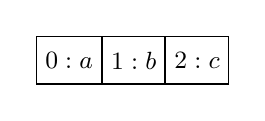
\begin{tikzpicture}
\small
\matrix[nodes={draw,minimum size=6mm}] {
  \node {$0:a$}; & \node {$1:b$}; & \node {$2:c$};\\
};
\end{tikzpicture}

\noindent shows an array with three elements. The value at position 0 is $a$; the
value at position 1 is $b$; the value at position 2 is $c$.

\subsection{{\tt{}\protect\nwindexuse{DBCreateNewInstance}{DBCreateNewInstance}{NW27XAxz-2CVxut-1}DBCreateNewInstance}(0)}
\begin{tabular}{p{\textwidth}}
\toprule
\rowcolor{TableTitle}
Method \textcolor{blue}{{\tt{}\protect\nwindexuse{DBCreateNewInstance}{DBCreateNewInstance}{NW27XAxz-2CVxut-1}DBCreateNewInstance}}(0) creates a new database
instance. It uses {\tt{}\protect\nwindexuse{setupDriver}{setupDriver}{NW27XAxz-33Wt2A-1}setupDriver}(0) to register the JDBC {\tt{}DriverManager} to
the new instance.  If the DBCP2 {\tt{}PoolingDriver} cannot be found, a
{\tt{}ClassNotFoundException} is thrown. We consider this exception to be fatal
and we exit immediately.  On the other hand if a {\tt{}SQLException} occurs, we
rethrow to let the caller handle it. This exception can occur if the driver
cannot access the database for whatever reason.\\
\midrule
\textbf{Parameters:} none.\\
\textbf{Returns:} nothing.\\
\textbf{Side Effects:} initializes a new in-memory Derby instance,
or exits the JVM if the DBCP2 driver
cannot be loaded.\\
\textbf{Throws:} {\tt{}SQLException} if database cannot be accessed for whatever
reason.\\
\bottomrule
\end{tabular}
\nwenddocs{}\nwbegincode{33}\sublabel{NW27XAxz-2CVxut-1}\nwmargintag{{\nwtagstyle{}\subpageref{NW27XAxz-2CVxut-1}}}\moddef{Initialize new empty database~{\nwtagstyle{}\subpageref{NW27XAxz-2CVxut-1}}}\endmoddef\nwalsodefined{\\{NW2ZDXo8-2CVxut-2}}\nwused{\\{NW27XAxz-4PbjF-3}\\{NW2ZDXo8-bF3Hn-1}}
public void DBCreateNewInstance() throws SQLException \{
  try \{
    this.setupDriver();
  \} catch (SQLException e) \{
    throw e;
  \} catch (ClassNotFoundException e) \{
    System.err.println("Storage.init(): "+\LA{}Err0~{\nwtagstyle{}\subpageref{NW27XAxz-15VC47-1}}\RA{});
    e.printStackTrace();
    System.exit(1);
  \}
\}
\nosublabel{NW27XAxz-2CVxut-1-u1}\nwindexdefn{DBCreateNewInstance}{DBCreateNewInstance}{NW27XAxz-2CVxut-1}\eatline
\nwidentdefs{\\{{DBCreateNewInstance}{DBCreateNewInstance}}}\nwidentuses{\\{{setupDriver}{setupDriver}}}\nwindexuse{setupDriver}{setupDriver}{NW27XAxz-2CVxut-1}\nwendcode{}\nwbegindocs{34}\nwdocspar
\subsection{{\tt{}\protect\nwindexuse{DBCloseInstance}{DBCloseInstance}{NW27XAxz-3A3oOU-1}DBCloseInstance}(0)}
\begin{tabular}{p{\textwidth}}
\toprule
\rowcolor{TableTitle}
Method \textcolor{blue}{{\tt{}\protect\nwindexuse{DBCloseInstance}{DBCloseInstance}{NW27XAxz-3A3oOU-1}DBCloseInstance}}(0) closes an existing Jargo
database instance.  If the instance closes successfully, a {\tt{}SQLException}
with error code {\tt{}45000} is thrown. Otherwise, some other error code is
thrown. In this case we rethrow to let the caller handle it.\\
\midrule
\textbf{Parameters:} none.\\
\textbf{Returns:} nothing.\\
\textbf{Side Effects:} closes an existing Jargo database instance.\\
\textbf{Throws:} {\tt{}SQLException} if database cannot be closed for whatever
reason.\\
\bottomrule
\end{tabular}
\nwenddocs{}\nwbegincode{35}\sublabel{NW27XAxz-3A3oOU-1}\nwmargintag{{\nwtagstyle{}\subpageref{NW27XAxz-3A3oOU-1}}}\moddef{Close database~{\nwtagstyle{}\subpageref{NW27XAxz-3A3oOU-1}}}\endmoddef\nwalsodefined{\\{NW2ZDXo8-3A3oOU-2}}\nwused{\\{NW27XAxz-4PbjF-3}\\{NW2ZDXo8-bF3Hn-1}}
public void DBCloseInstance() throws SQLException \{
  try \{
    DriverManager.getConnection("jdbc:derby:memory:jargo;drop=true");
  \} catch (SQLException e) \{
    if (e.getErrorCode() != 45000) \{
      throw e;
    \}
  \}
\}
\nwindexdefn{DBCloseInstance}{DBCloseInstance}{NW27XAxz-3A3oOU-1}\eatline
\nwidentdefs{\\{{DBCloseInstance}{DBCloseInstance}}}\nwendcode{}\nwbegindocs{36}\nwdocspar
\subsection{{\tt{}\protect\nwindexuse{getReferenceVerticesCache}{getReferenceVerticesCache}{NW27XAxz-21qmOa-1}getReferenceVerticesCache}(0)}
\begin{tabular}{p{\textwidth}}
\toprule
\rowcolor{TableTitle}
Method \textcolor{blue}{{\tt{}\protect\nwindexuse{getReferenceVerticesCache}{getReferenceVerticesCache}{NW27XAxz-21qmOa-1}getReferenceVerticesCache}}(0) returns a read-only
reference to {\tt{}\protect\nwindexuse{lu{\char95}vertices}{lu:unvertices}{NW27XAxz-17yXws-2}lu{\char95}vertices}.\\
\midrule
\textbf{Parameters:} none.\\
\textbf{Returns:} a read-only reference to {\tt{}\protect\nwindexuse{lu{\char95}vertices}{lu:unvertices}{NW27XAxz-17yXws-2}lu{\char95}vertices}.\\
\textbf{Side Effects:} none.\\
\textbf{Throws:} nothing.\\
\bottomrule
\end{tabular}
\nwenddocs{}\nwbegincode{37}\sublabel{NW27XAxz-21qmOa-1}\nwmargintag{{\nwtagstyle{}\subpageref{NW27XAxz-21qmOa-1}}}\moddef{Get reference to vertices cache~{\nwtagstyle{}\subpageref{NW27XAxz-21qmOa-1}}}\endmoddef\nwalsodefined{\\{NWvbkzY-21qmOa-2}}\nwused{\\{NW27XAxz-4PbjF-3}\\{NWvbkzY-3YjONp-1}}
public final ConcurrentHashMap<Integer, int[]> getReferenceVerticesCache() \{
  return this.lu_vertices;
\}
\nwindexdefn{getReferenceVerticesCache}{getReferenceVerticesCache}{NW27XAxz-21qmOa-1}\eatline
\nwidentdefs{\\{{getReferenceVerticesCache}{getReferenceVerticesCache}}}\nwidentuses{\\{{lu{\char95}vertices}{lu:unvertices}}}\nwindexuse{lu{\char95}vertices}{lu:unvertices}{NW27XAxz-21qmOa-1}\nwendcode{}\nwbegindocs{38}\nwdocspar
\subsection{{\tt{}\protect\nwindexuse{getReferenceEdgesCache}{getReferenceEdgesCache}{NW27XAxz-3KzwIy-1}getReferenceEdgesCache}(0)}
\begin{tabular}{p{\textwidth}}
\toprule
\rowcolor{TableTitle}
Method \textcolor{blue}{{\tt{}\protect\nwindexuse{getReferenceEdgesCache}{getReferenceEdgesCache}{NW27XAxz-3KzwIy-1}getReferenceEdgesCache}}(0) returns a read-only
reference to {\tt{}\protect\nwindexuse{lu{\char95}edges}{lu:unedges}{NW27XAxz-17yXws-2}lu{\char95}edges}.\\
\midrule
\textbf{Parameters:} none.\\
\textbf{Returns:} a read-only reference to {\tt{}\protect\nwindexuse{lu{\char95}edges}{lu:unedges}{NW27XAxz-17yXws-2}lu{\char95}edges}.\\
\textbf{Side Effects:} none.\\
\textbf{Throws:} nothing.\\
\bottomrule
\end{tabular}
\nwenddocs{}\nwbegincode{39}\sublabel{NW27XAxz-3KzwIy-1}\nwmargintag{{\nwtagstyle{}\subpageref{NW27XAxz-3KzwIy-1}}}\moddef{Get reference to edges cache~{\nwtagstyle{}\subpageref{NW27XAxz-3KzwIy-1}}}\endmoddef\nwalsodefined{\\{NWvbkzY-3KzwIy-2}}\nwused{\\{NW27XAxz-4PbjF-3}\\{NWvbkzY-3YjONp-1}}
public final ConcurrentHashMap<Integer,
    ConcurrentHashMap<Integer, int[]>> getReferenceEdgesCache() \{
  return this.lu_edges;
\}
\nwindexdefn{getReferenceEdgesCache}{getReferenceEdgesCache}{NW27XAxz-3KzwIy-1}\eatline
\nwidentdefs{\\{{getReferenceEdgesCache}{getReferenceEdgesCache}}}\nwidentuses{\\{{lu{\char95}edges}{lu:unedges}}}\nwindexuse{lu{\char95}edges}{lu:unedges}{NW27XAxz-3KzwIy-1}\nwendcode{}\nwbegindocs{40}\nwdocspar
\subsection{{\tt{}\protect\nwindexuse{getReferenceUsersCache}{getReferenceUsersCache}{NW27XAxz-1EJdXT-1}getReferenceUsersCache}(0)}
\begin{tabular}{p{\textwidth}}
\toprule
\rowcolor{TableTitle}
Method \textcolor{blue}{{\tt{}\protect\nwindexuse{getReferenceUsersCache}{getReferenceUsersCache}{NW27XAxz-1EJdXT-1}getReferenceUsersCache}}(0) returns a read-only
reference to {\tt{}\protect\nwindexuse{lu{\char95}users}{lu:unusers}{NW27XAxz-17yXws-2}lu{\char95}users}.\\
\midrule
\textbf{Parameters:} none.\\
\textbf{Returns:} a read-only reference to {\tt{}\protect\nwindexuse{lu{\char95}users}{lu:unusers}{NW27XAxz-17yXws-2}lu{\char95}users}.\\
\textbf{Side Effects:} none.\\
\textbf{Throws:} nothing.\\
\bottomrule
\end{tabular}
\nwenddocs{}\nwbegincode{41}\sublabel{NW27XAxz-1EJdXT-1}\nwmargintag{{\nwtagstyle{}\subpageref{NW27XAxz-1EJdXT-1}}}\moddef{Get reference to users cache~{\nwtagstyle{}\subpageref{NW27XAxz-1EJdXT-1}}}\endmoddef\nwalsodefined{\\{NWvbkzY-1EJdXT-2}}\nwused{\\{NW27XAxz-4PbjF-3}\\{NWvbkzY-3YjONp-1}}
public final ConcurrentHashMap<Integer, int[]> getReferenceUsersCache() \{
  return this.lu_users;
\}
\nwindexdefn{getReferenceUsersCache}{getReferenceUsersCache}{NW27XAxz-1EJdXT-1}\eatline
\nwidentdefs{\\{{getReferenceUsersCache}{getReferenceUsersCache}}}\nwidentuses{\\{{lu{\char95}users}{lu:unusers}}}\nwindexuse{lu{\char95}users}{lu:unusers}{NW27XAxz-1EJdXT-1}\nwendcode{}\nwbegindocs{42}\nwdocspar
\subsection{{\tt{}\protect\nwindexuse{DBLoadDataModel}{DBLoadDataModel}{NW27XAxz-4P4YpK-1}DBLoadDataModel}(0)}
\begin{tabular}{p{\textwidth}}
\toprule
\rowcolor{TableTitle}
Method \textcolor{blue}{{\tt{}\protect\nwindexuse{DBLoadDataModel}{DBLoadDataModel}{NW27XAxz-4P4YpK-1}DBLoadDataModel}}(0) loads the data model in
\S\ref{sec:ridesharing-data-model} into the Jargo database instance. If the
data model cannot be loaded, a {\tt{}SQLException} is thrown. We consider this
exception to be fatal and we exit immediately. Possible reasons for such an
exception might be because the caller forgot to first call
{\tt{}\protect\nwindexuse{DBCreateNewInstance}{DBCreateNewInstance}{NW27XAxz-2CVxut-1}DBCreateNewInstance}(0) resulting in ``No suitable driver found'' (error
code 0), or because the caller previously called {\tt{}\protect\nwindexuse{DBLoadBackup}{DBLoadBackup}{NW27XAxz-b3Hn1-1}DBLoadBackup}(1) resulting
in ``Table/View V already exists'' (error code 20000). In either case we print
a hint to terminal to guide the debugging.\\
\midrule
\textbf{Parameters:} none.\\
\textbf{Returns:} nothing.\\
\textbf{Side Effects:} loads the data model in \S\ref{sec:ridesharing-data-model}
into the Jargo instance, or exits the JVM if failure occurs.\\
\textbf{Throws:} nothing.\\
\bottomrule
\end{tabular}
\nwenddocs{}\nwbegincode{43}\sublabel{NW27XAxz-4P4YpK-1}\nwmargintag{{\nwtagstyle{}\subpageref{NW27XAxz-4P4YpK-1}}}\moddef{Load data model~{\nwtagstyle{}\subpageref{NW27XAxz-4P4YpK-1}}}\endmoddef\nwalsodefined{\\{NW2ZDXo8-4P4YpK-2}}\nwused{\\{NW27XAxz-4PbjF-3}\\{NW2ZDXo8-bF3Hn-1}}
public void DBLoadDataModel() \{
  try (\LA{}Open \code{}conn\edoc{}~{\nwtagstyle{}\subpageref{NW27XAxz-JT1v9-1}}\RA{}) \{
    Statement stmt = conn.createStatement();
    stmt.clearBatch();
    stmt.addBatch(\LA{}Create Table V statement~{\nwtagstyle{}\subpageref{NW27XAxz-RzwV3-1}}\RA{});
    stmt.addBatch(\LA{}Create Table E statement~{\nwtagstyle{}\subpageref{NW27XAxz-2WHSWQ-1}}\RA{});
    stmt.addBatch(\LA{}Create Table UQ statement~{\nwtagstyle{}\subpageref{NW27XAxz-llmAG-1}}\RA{});
    stmt.addBatch(\LA{}Create Table UE statement~{\nwtagstyle{}\subpageref{NW27XAxz-sBCgz-1}}\RA{});
    stmt.addBatch(\LA{}Create Table UL statement~{\nwtagstyle{}\subpageref{NW27XAxz-3Q8NSk-1}}\RA{});
    stmt.addBatch(\LA{}Create Table UO statement~{\nwtagstyle{}\subpageref{NW27XAxz-qCW00-1}}\RA{});
    stmt.addBatch(\LA{}Create Table UD statement~{\nwtagstyle{}\subpageref{NW27XAxz-1OVMyH-1}}\RA{});
    stmt.addBatch(\LA{}Create Table UB statement~{\nwtagstyle{}\subpageref{NW27XAxz-3QSM5L-1}}\RA{});
    stmt.addBatch(\LA{}Create Table S statement~{\nwtagstyle{}\subpageref{NW27XAxz-2D0DN7-1}}\RA{});
    stmt.addBatch(\LA{}Create Table R statement~{\nwtagstyle{}\subpageref{NW27XAxz-Uo9HJ-1}}\RA{});
    stmt.addBatch(\LA{}Create Table W statement~{\nwtagstyle{}\subpageref{NW27XAxz-2FnbXJ-1}}\RA{});
    stmt.addBatch(\LA{}Create Table PD statement~{\nwtagstyle{}\subpageref{NW27XAxz-1aGcZB-1}}\RA{});
    stmt.addBatch(\LA{}Create Table CW statement~{\nwtagstyle{}\subpageref{NW27XAxz-2HehGp-1}}\RA{});
    stmt.addBatch(\LA{}Create Table CPD statement~{\nwtagstyle{}\subpageref{NW27XAxz-q5ofx-1}}\RA{});
    stmt.addBatch(\LA{}Create Table CQ statement~{\nwtagstyle{}\subpageref{NW27XAxz-2YsMAX-1}}\RA{});
    stmt.addBatch(\LA{}Create View r\_user statement~{\nwtagstyle{}\subpageref{NW27XAxz-35s8QT-1}}\RA{});
    stmt.addBatch(\LA{}Create View r\_server statement~{\nwtagstyle{}\subpageref{NW27XAxz-3E22nZ-1}}\RA{});
    stmt.addBatch(\LA{}Create View f\_distance\_blocks statement~{\nwtagstyle{}\subpageref{NW27XAxz-2SQlWK-1}}\RA{});
    stmt.addBatch(\LA{}Create View f\_status statement (Eq.~\ref{eq:status})~{\nwtagstyle{}\subpageref{NW27XAxz-qqtLb-1}}\RA{});
    stmt.addBatch(\LA{}Create View assignments statement (Eq.~\ref{eq:assignments})~{\nwtagstyle{}\subpageref{NW27XAxz-4DFJnJ-1}}\RA{});
    stmt.addBatch(\LA{}Create View assignments\_r statement (Eq.~\ref{eq:assigned-requests})~{\nwtagstyle{}\subpageref{NW27XAxz-4Me5rv-1}}\RA{});
    stmt.addBatch(\LA{}Create View service\_rate statement (Eq.~\ref{eq:service-rate})~{\nwtagstyle{}\subpageref{NW27XAxz-3taWHj-1}}\RA{});
    stmt.addBatch(\LA{}Create View dist\_base statement (Eq.~\ref{eq:base-distance})~{\nwtagstyle{}\subpageref{NW27XAxz-Xwf4i-1}}\RA{});
    stmt.addBatch(\LA{}Create View dist\_s\_travel statement~{\nwtagstyle{}\subpageref{NW27XAxz-I0bnu-1}}\RA{});
    stmt.addBatch(\LA{}Create View dist\_s\_cruising statement (Eq.~\ref{eq:cruising-distance})~{\nwtagstyle{}\subpageref{NW27XAxz-sPBsa-1}}\RA{});
    stmt.addBatch(\LA{}Create View dist\_s\_service statement (Eq.~\ref{eq:service-distance})~{\nwtagstyle{}\subpageref{NW27XAxz-21lyOa-1}}\RA{});
    stmt.addBatch(\LA{}Create View dist\_s\_base statement~{\nwtagstyle{}\subpageref{NW27XAxz-15VZds-1}}\RA{});
    stmt.addBatch(\LA{}Create View dist\_r\_base statement~{\nwtagstyle{}\subpageref{NW27XAxz-2qZ1kZ-1}}\RA{});
    stmt.addBatch(\LA{}Create View dist\_r\_unassigned statement~{\nwtagstyle{}\subpageref{NW27XAxz-20Wo4P-1}}\RA{});
    stmt.addBatch(\LA{}Create View dist\_r\_transit statement (Eq.~\ref{eq:transit-distance})~{\nwtagstyle{}\subpageref{NW27XAxz-eXH6J-1}}\RA{});
    stmt.addBatch(\LA{}Create View dist\_r\_detour statement (Eq.~\ref{eq:detour-distance})~{\nwtagstyle{}\subpageref{NW27XAxz-4OnMrk-1}}\RA{});
    stmt.addBatch(\LA{}Create View dur\_s\_travel statement~{\nwtagstyle{}\subpageref{NW27XAxz-3sQlba-1}}\RA{});
    stmt.addBatch(\LA{}Create View dur\_r\_pickup statement (Eq.~\ref{eq:pick-up delay})~{\nwtagstyle{}\subpageref{NW27XAxz-34NkTM-1}}\RA{});
    stmt.addBatch(\LA{}Create View dur\_r\_transit statement (Eq.~\ref{eq:transit-duration})~{\nwtagstyle{}\subpageref{NW27XAxz-Puojq-1}}\RA{});
    stmt.addBatch(\LA{}Create View dur\_r\_travel statement (Eq.~\ref{eq:travel-duration})~{\nwtagstyle{}\subpageref{NW27XAxz-3a0WDv-1}}\RA{});
    stmt.addBatch(\LA{}Create View t\_r\_depart statement (Eq.~\ref{eq:departure-time})~{\nwtagstyle{}\subpageref{NW27XAxz-45SyYZ-1}}\RA{});
    stmt.addBatch(\LA{}Create View t\_s\_depart statement (Eq.~\ref{eq:departure-time})~{\nwtagstyle{}\subpageref{NW27XAxz-2riY0r-1}}\RA{});
    stmt.addBatch(\LA{}Create View t\_r\_arrive statement (Eq.~\ref{eq:arrival-time})~{\nwtagstyle{}\subpageref{NW27XAxz-28E5sQ-1}}\RA{});
    stmt.addBatch(\LA{}Create View t\_s\_arrive statement (Eq.~\ref{eq:arrival-time})~{\nwtagstyle{}\subpageref{NW27XAxz-3oL4CY-1}}\RA{});
    stmt.addBatch("CREATE INDEX W_sid_t1 ON W (sid, t1)");
    stmt.addBatch("CREATE INDEX W_sid_t2 ON W (sid, t2)");
    stmt.addBatch("CREATE INDEX W_sid_v2 ON W (sid, v2)");
    stmt.addBatch("CREATE INDEX W_sid_t1_t2 ON W (sid, t1, t2)");
    stmt.executeBatch();
    conn.commit();
  \} catch (SQLException e) \{
    System.err.println("Storage.DBLoadDataModel(): "+\LA{}Err0~{\nwtagstyle{}\subpageref{NW27XAxz-15VC47-1}}\RA{});
    if (e.getErrorCode() == 0) \{
      System.err.println("(did you forget to call Storage.DBCreateNewInstance()?)");
    \} else if (e.getErrorCode() == 20000) \{
      System.err.println("(data model already exists from Storage.DBLoadBackup()?)");
    \}
    e.printStackTrace(System.err);
    System.exit(1);
  \}
\}
\nwindexdefn{DBLoadDataModel}{DBLoadDataModel}{NW27XAxz-4P4YpK-1}\eatline
\nwidentdefs{\\{{DBLoadDataModel}{DBLoadDataModel}}}\nwidentuses{\\{{DBCreateNewInstance}{DBCreateNewInstance}}\\{{DBLoadBackup}{DBLoadBackup}}}\nwindexuse{DBCreateNewInstance}{DBCreateNewInstance}{NW27XAxz-4P4YpK-1}\nwindexuse{DBLoadBackup}{DBLoadBackup}{NW27XAxz-4P4YpK-1}\nwendcode{}\nwbegindocs{44}\nwdocspar
\subsection{{\tt{}\protect\nwindexuse{DBLoadBackup}{DBLoadBackup}{NW27XAxz-b3Hn1-1}DBLoadBackup}(1)}
\begin{tabular}{p{\textwidth}}
\toprule
\rowcolor{TableTitle}
Method \textcolor{blue}{{\tt{}\protect\nwindexuse{DBLoadBackup}{DBLoadBackup}{NW27XAxz-b3Hn1-1}DBLoadBackup}}(1) loads a previously saved Jargo
database instance from disk into working memory. It uses {\tt{}\protect\nwindexuse{setupDriver}{setupDriver}{NW27XAxz-33Wt2A-1}setupDriver}(0) to
register the JDBC {\tt{}DriverManager} to the new instance.  If the DBCP2
{\tt{}PoolingDriver} cannot be found, a {\tt{}ClassNotFoundException} is thrown. We
consider this exception to be fatal and we exit immediately.  On the other hand
if a {\tt{}SQLException} occurs, we rethrow to let the caller handle it. This
exception can occur if the driver cannot access the database for whatever
reason.\\
\midrule
\textbf{Parameters:} \\
\hspace{2mm} String {\tt{}p} (param. 1): path to directory where backup is located.\\
\textbf{Returns:} nothing.\\
\textbf{Side Effects:} loads backup into Jargo database instance, or exits the
JVM if failure occurs.\\
\textbf{Throws:} {\tt{}SQLException} if database cannot be accessed, or
{\tt{}ClassNotFoundException} if the DBCP2 driver cannot be found.\\
\bottomrule
\end{tabular}
\nwenddocs{}\nwbegincode{45}\sublabel{NW27XAxz-b3Hn1-1}\nwmargintag{{\nwtagstyle{}\subpageref{NW27XAxz-b3Hn1-1}}}\moddef{Load backup~{\nwtagstyle{}\subpageref{NW27XAxz-b3Hn1-1}}}\endmoddef\nwalsodefined{\\{NW2ZDXo8-b3Hn1-2}}\nwused{\\{NW27XAxz-4PbjF-3}\\{NW2ZDXo8-bF3Hn-1}}
public void DBLoadBackup(final String p) throws SQLException \{
  this.CONNECTIONS_URL = "jdbc:derby:memory:jargo;createFrom="+p;
  try \{
    this.setupDriver();
  \} catch (ClassNotFoundException e) \{
    System.out.println("Storage.DBLoadBackup(1): "+\LA{}Err0~{\nwtagstyle{}\subpageref{NW27XAxz-15VC47-1}}\RA{});
    e.printStackTrace();
    System.exit(1);
  \}
\}
\nosublabel{NW27XAxz-b3Hn1-1-u1}\nwindexdefn{DBLoadBackup}{DBLoadBackup}{NW27XAxz-b3Hn1-1}\eatline
\nwidentdefs{\\{{DBLoadBackup}{DBLoadBackup}}}\nwidentuses{\\{{CONNECTIONS{\char95}URL}{CONNECTIONS:unURL}}\\{{setupDriver}{setupDriver}}}\nwindexuse{CONNECTIONS{\char95}URL}{CONNECTIONS:unURL}{NW27XAxz-b3Hn1-1}\nwindexuse{setupDriver}{setupDriver}{NW27XAxz-b3Hn1-1}\nwendcode{}\nwbegindocs{46}\nwdocspar
\subsection{{\tt{}\protect\nwindexuse{DBLoadRoadNetworkFromDB}{DBLoadRoadNetworkFromDB}{NW27XAxz-2gRGj0-1}DBLoadRoadNetworkFromDB}(0)}
\begin{tabular}{p{\textwidth}}
\toprule
\rowcolor{TableTitle}
Method \textcolor{blue}{{\tt{}\protect\nwindexuse{DBLoadRoadNetworkFromDB}{DBLoadRoadNetworkFromDB}{NW27XAxz-2gRGj0-1}DBLoadRoadNetworkFromDB}}(0) loads the
two caches {\tt{}\protect\nwindexuse{lu{\char95}vertices}{lu:unvertices}{NW27XAxz-17yXws-2}lu{\char95}vertices} and {\tt{}\protect\nwindexuse{lu{\char95}edges}{lu:unedges}{NW27XAxz-17yXws-2}lu{\char95}edges} using the vertices and edges
data in Tables V and E in the database. If queries on Tables V and E
fail, this method throws a {\tt{}SQLException}.
\\
\midrule
\textbf{Parameters:} none.\\
\textbf{Returns:} nothing.\\
\textbf{Side Effects:} populates {\tt{}\protect\nwindexuse{lu{\char95}vertices}{lu:unvertices}{NW27XAxz-17yXws-2}lu{\char95}vertices} and {\tt{}\protect\nwindexuse{lu{\char95}edges}{lu:unedges}{NW27XAxz-17yXws-2}lu{\char95}edges}.\\
\textbf{Throws:} {\tt{}SQLException} if Tables V and E cannot be queried or
other database failure is encountered.\\
\bottomrule
\end{tabular}
\nwenddocs{}\nwbegincode{47}\sublabel{NW27XAxz-2gRGj0-1}\nwmargintag{{\nwtagstyle{}\subpageref{NW27XAxz-2gRGj0-1}}}\moddef{Load road network from database~{\nwtagstyle{}\subpageref{NW27XAxz-2gRGj0-1}}}\endmoddef\nwalsodefined{\\{NW27XAxz-2gRGj0-2}\\{NW27XAxz-2gRGj0-3}\\{NW27XAxz-2gRGj0-4}\\{NW27XAxz-2gRGj0-5}}\nwused{\\{NW27XAxz-4PbjF-3}}
public void DBLoadRoadNetworkFromDB() throws SQLException \{
\nwindexdefn{DBLoadRoadNetworkFromDB}{DBLoadRoadNetworkFromDB}{NW27XAxz-2gRGj0-1}\eatline
\nwidentdefs{\\{{DBLoadRoadNetworkFromDB}{DBLoadRoadNetworkFromDB}}}\nwendcode{}\nwbegindocs{48}{\small Our approach is to create two temporary maps on the heap, populate the
temporary maps, then assign {\tt{}\protect\nwindexuse{lu{\char95}vertices}{lu:unvertices}{NW27XAxz-17yXws-2}lu{\char95}vertices} and {\tt{}\protect\nwindexuse{lu{\char95}edges}{lu:unedges}{NW27XAxz-17yXws-2}lu{\char95}edges} to reference the
temporary maps if all succeeds. This way we don't corrupt {\tt{}\protect\nwindexuse{lu{\char95}vertices}{lu:unvertices}{NW27XAxz-17yXws-2}lu{\char95}vertices} and
{\tt{}\protect\nwindexuse{lu{\char95}edges}{lu:unedges}{NW27XAxz-17yXws-2}lu{\char95}edges} in case of failure. (The approach might be overly cautious as it's
hard to imagine why this method would ever be called if the caches are already
populated.)}
\nwenddocs{}\nwbegincode{49}\sublabel{NW27XAxz-2gRGj0-2}\nwmargintag{{\nwtagstyle{}\subpageref{NW27XAxz-2gRGj0-2}}}\moddef{Load road network from database~{\nwtagstyle{}\subpageref{NW27XAxz-2gRGj0-1}}}\plusendmoddef
  ConcurrentHashMap<Integer, int[]>    lu1 = new ConcurrentHashMap<>();
  ConcurrentHashMap<Integer,
    ConcurrentHashMap<Integer, int[]>> lu2 = new ConcurrentHashMap<>();
\nwendcode{}\nwbegindocs{50}\nwdocspar
{\small We start by querying the vertices.}
\nwenddocs{}\nwbegincode{51}\sublabel{NW27XAxz-2gRGj0-3}\nwmargintag{{\nwtagstyle{}\subpageref{NW27XAxz-2gRGj0-3}}}\moddef{Load road network from database~{\nwtagstyle{}\subpageref{NW27XAxz-2gRGj0-1}}}\plusendmoddef
  try \{
    final int[] output = this.DBQueryAllVertices();
    for (int i = 0; i < (output.length - 2); i += 3) \{
      final int   v = output[(i + 0)];
      final int lng = output[(i + 1)];
      final int lat = output[(i + 2)];
      lu1.put(v, new int[] \{ lng, lat \});
    \}
  \} catch (SQLException e) \{
    throw e;
  \}
\nwidentuses{\\{{DBQueryAllVertices}{DBQueryAllVertices}}}\nwindexuse{DBQueryAllVertices}{DBQueryAllVertices}{NW27XAxz-2gRGj0-3}\nwendcode{}\nwbegindocs{52}\nwdocspar
{\small Then we go on to query the edges.}
\nwenddocs{}\nwbegincode{53}\sublabel{NW27XAxz-2gRGj0-4}\nwmargintag{{\nwtagstyle{}\subpageref{NW27XAxz-2gRGj0-4}}}\moddef{Load road network from database~{\nwtagstyle{}\subpageref{NW27XAxz-2gRGj0-1}}}\plusendmoddef
  try \{
    final int[] output = this.DBQueryAllEdges();
    for (int i = 0; i < (output.length - 3); i += 4) \{
      final int v1 = output[(i + 0)];
      final int v2 = output[(i + 1)];
      final int dd = output[(i + 2)];
      final int nu = output[(i + 3)];
      if (!lu2.containsKey(v1)) \{
        lu2.put(v1, new ConcurrentHashMap());
      \}
      lu2.get(v1).put(v2, new int[] \{ dd, nu \});
    \}
  \} catch (SQLException e) \{
    throw e;
  \}
\nwidentuses{\\{{DBQueryAllEdges}{DBQueryAllEdges}}}\nwindexuse{DBQueryAllEdges}{DBQueryAllEdges}{NW27XAxz-2gRGj0-4}\nwendcode{}\nwbegindocs{54}\nwdocspar
{\small Finally we do the assignment.}
\nwenddocs{}\nwbegincode{55}\sublabel{NW27XAxz-2gRGj0-5}\nwmargintag{{\nwtagstyle{}\subpageref{NW27XAxz-2gRGj0-5}}}\moddef{Load road network from database~{\nwtagstyle{}\subpageref{NW27XAxz-2gRGj0-1}}}\plusendmoddef
  this.lu_vertices = lu1;
  this.lu_edges    = lu2;
\}
\nwidentuses{\\{{lu{\char95}edges}{lu:unedges}}\\{{lu{\char95}vertices}{lu:unvertices}}}\nwindexuse{lu{\char95}edges}{lu:unedges}{NW27XAxz-2gRGj0-5}\nwindexuse{lu{\char95}vertices}{lu:unvertices}{NW27XAxz-2gRGj0-5}\nwendcode{}\nwbegindocs{56}\nwdocspar

\subsection{{\tt{}\protect\nwindexuse{DBLoadUsersFromDB}{DBLoadUsersFromDB}{NW27XAxz-3TLCwk-1}DBLoadUsersFromDB}(0)}
\begin{tabular}{p{\textwidth}}
\toprule
\rowcolor{TableTitle}
Method \textcolor{blue}{{\tt{}\protect\nwindexuse{DBLoadUsersFromDB}{DBLoadUsersFromDB}{NW27XAxz-3TLCwk-1}DBLoadUsersFromDB}}(0) loads the two caches
{\tt{}\protect\nwindexuse{lu{\char95}users}{lu:unusers}{NW27XAxz-17yXws-2}lu{\char95}users} and {\tt{}\protect\nwindexuse{lu{\char95}rstatus}{lu:unrstatus}{NW27XAxz-17yXws-1}lu{\char95}rstatus} using data in the user and assignment tables in
the database. If queries on these tables fail, this method throws a
{\tt{}SQLException}.\\
\midrule
\textbf{Parameters:} none.\\
\textbf{Returns:} nothing.\\
\textbf{Side Effects:} populates {\tt{}\protect\nwindexuse{lu{\char95}users}{lu:unusers}{NW27XAxz-17yXws-2}lu{\char95}users} and {\tt{}\protect\nwindexuse{lu{\char95}rstatus}{lu:unrstatus}{NW27XAxz-17yXws-1}lu{\char95}rstatus}.\\
\textbf{Throws:} {\tt{}SQLException} if user and assignment tables cannot be
queried or other database failure is encountered.\\
\bottomrule
\end{tabular}
\nwenddocs{}\nwbegincode{57}\sublabel{NW27XAxz-3TLCwk-1}\nwmargintag{{\nwtagstyle{}\subpageref{NW27XAxz-3TLCwk-1}}}\moddef{Load users from database~{\nwtagstyle{}\subpageref{NW27XAxz-3TLCwk-1}}}\endmoddef\nwalsodefined{\\{NW27XAxz-3TLCwk-2}\\{NW27XAxz-3TLCwk-3}\\{NW27XAxz-3TLCwk-4}\\{NW27XAxz-3TLCwk-5}}\nwused{\\{NW27XAxz-4PbjF-3}}
public void DBLoadUsersFromDB() throws SQLException \{
\nwindexdefn{DBLoadUsersFromDB}{DBLoadUsersFromDB}{NW27XAxz-3TLCwk-1}\eatline
\nwidentdefs{\\{{DBLoadUsersFromDB}{DBLoadUsersFromDB}}}\nwendcode{}\nwbegindocs{58}{\small Our approach follows the approach for {\tt{}\protect\nwindexuse{DBLoadRoadNetworkFromDB}{DBLoadRoadNetworkFromDB}{NW27XAxz-2gRGj0-1}DBLoadRoadNetworkFromDB}(0).
We start by creating two temporary maps on the heap.}
\nwenddocs{}\nwbegincode{59}\sublabel{NW27XAxz-3TLCwk-2}\nwmargintag{{\nwtagstyle{}\subpageref{NW27XAxz-3TLCwk-2}}}\moddef{Load users from database~{\nwtagstyle{}\subpageref{NW27XAxz-3TLCwk-1}}}\plusendmoddef
  ConcurrentHashMap<Integer, int[]> lu1 = new ConcurrentHashMap<>();
  Map<Integer, Boolean>             lu2 = new HashMap<>();
\nwendcode{}\nwbegindocs{60}\nwdocspar
{\small Then we query the users.}
\nwenddocs{}\nwbegincode{61}\sublabel{NW27XAxz-3TLCwk-3}\nwmargintag{{\nwtagstyle{}\subpageref{NW27XAxz-3TLCwk-3}}}\moddef{Load users from database~{\nwtagstyle{}\subpageref{NW27XAxz-3TLCwk-1}}}\plusendmoddef
  try \{
    final int[] output = this.DBQueryAllUsers();
    for (int i = 0; i < (output.length - 6); i += 7) \{
      final int uid = output[(i + 0)];
      final int  uq = output[(i + 1)];
      final int  ue = output[(i + 2)];
      final int  ul = output[(i + 3)];
      final int  uo = output[(i + 4)];
      final int  ud = output[(i + 5)];
      final int  ub = output[(i + 6)];
      lu1.put(uid, new int[] \{ uid, uq, ue, ul, uo, ud, ub \});
\nwidentuses{\\{{DBQueryAllUsers}{DBQueryAllUsers}}}\nwindexuse{DBQueryAllUsers}{DBQueryAllUsers}{NW27XAxz-3TLCwk-3}\nwendcode{}\nwbegindocs{62}\nwdocspar
{\small If the user is a request, in other words the user load is positive,
we query the request's assignment status.}
\nwenddocs{}\nwbegincode{63}\sublabel{NW27XAxz-3TLCwk-4}\nwmargintag{{\nwtagstyle{}\subpageref{NW27XAxz-3TLCwk-4}}}\moddef{Load users from database~{\nwtagstyle{}\subpageref{NW27XAxz-3TLCwk-1}}}\plusendmoddef
      if (uq > 0) \{
        lu2.put(uid, (this.DBQueryRequestIsAssigned(uid).length > 0 ? true : false));
      \}
    \}
  \} catch (SQLException e) \{
    throw e;
  \}
\nwidentuses{\\{{DBQueryRequestIsAssigned}{DBQueryRequestIsAssigned}}}\nwindexuse{DBQueryRequestIsAssigned}{DBQueryRequestIsAssigned}{NW27XAxz-3TLCwk-4}\nwendcode{}\nwbegindocs{64}\nwdocspar
{\small Finally we do the assignment.}
\nwenddocs{}\nwbegincode{65}\sublabel{NW27XAxz-3TLCwk-5}\nwmargintag{{\nwtagstyle{}\subpageref{NW27XAxz-3TLCwk-5}}}\moddef{Load users from database~{\nwtagstyle{}\subpageref{NW27XAxz-3TLCwk-1}}}\plusendmoddef
  this.lu_users   = lu1;
  this.lu_rstatus = lu2;
\}
\nwidentuses{\\{{lu{\char95}rstatus}{lu:unrstatus}}\\{{lu{\char95}users}{lu:unusers}}}\nwindexuse{lu{\char95}rstatus}{lu:unrstatus}{NW27XAxz-3TLCwk-5}\nwindexuse{lu{\char95}users}{lu:unusers}{NW27XAxz-3TLCwk-5}\nwendcode{}\nwbegindocs{66}\nwdocspar

\subsection{{\tt{}\protect\nwindexuse{DBSaveBackup}{DBSaveBackup}{NW27XAxz-2OKmqF-1}DBSaveBackup}(1)}
\begin{tabular}{p{\textwidth}}
\toprule
\rowcolor{TableTitle}
Method \textcolor{blue}{{\tt{}\protect\nwindexuse{DBSaveBackup}{DBSaveBackup}{NW27XAxz-2OKmqF-1}DBSaveBackup}}(1) exports the Jargo database
instance to disk. If a {\tt{}SQLException} occurs, we rethrow to let the caller
handle it.\\
\midrule
\textbf{Parameters:} \\
\hspace{2mm} String {\tt{}p} (param. 1): path to directory where instance should
be exported to.\\
\textbf{Returns:} nothing.\\
\textbf{Side Effects:} writes the database to disk.\\
\textbf{Throws:} {\tt{}SQLException} if failure is encountered.\\
\bottomrule
\end{tabular}
\nwenddocs{}\nwbegincode{67}\sublabel{NW27XAxz-2OKmqF-1}\nwmargintag{{\nwtagstyle{}\subpageref{NW27XAxz-2OKmqF-1}}}\moddef{Save backup~{\nwtagstyle{}\subpageref{NW27XAxz-2OKmqF-1}}}\endmoddef\nwalsodefined{\\{NW2ZDXo8-2OKmqF-2}}\nwused{\\{NW27XAxz-4PbjF-3}\\{NW2ZDXo8-bF3Hn-1}}
public void DBSaveBackup(final String p) throws SQLException \{
  try (\LA{}Open \code{}conn\edoc{}~{\nwtagstyle{}\subpageref{NW27XAxz-JT1v9-1}}\RA{}) \{
    CallableStatement cs = conn.prepareCall("CALL SYSCS_UTIL.SYSCS_BACKUP_DATABASE('"+p+"')");
    cs.execute();
  \} catch (SQLException e) \{
    throw e;
  \}
\}
\nosublabel{NW27XAxz-2OKmqF-1-u1}\nwindexdefn{DBSaveBackup}{DBSaveBackup}{NW27XAxz-2OKmqF-1}\eatline
\nwidentdefs{\\{{DBSaveBackup}{DBSaveBackup}}}\nwendcode{}\nwbegindocs{68}\nwdocspar
\subsection{{\tt{}{\char95}printSQLDriverStatistics}(0)}
\begin{tabular}{p{\textwidth}}
\toprule
\rowcolor{TableTitle}
FOR INTERNAL USE. Method \textcolor{blue}{{\tt{}{\char95}printSQLDriverStatistics}}(0)
prints the number of active and idle connections in the JDBC connection pool.
The following code comes from the Apache DBCP2 examples and is licensed by the
Apache Software Foundation.\\
\midrule
\textbf{Parameters:} none.\\
\textbf{Returns:} nothing.\\
\textbf{Side Effects:} prints number of active and idle connections.\\
\textbf{Throws:} {\tt{}SQLException} if failure occurs.\\
\bottomrule
\end{tabular}
\nwenddocs{}\nwbegincode{69}\sublabel{NW27XAxz-1lVtry-1}\nwmargintag{{\nwtagstyle{}\subpageref{NW27XAxz-1lVtry-1}}}\moddef{Print SQL driver statistics~{\nwtagstyle{}\subpageref{NW27XAxz-1lVtry-1}}}\endmoddef\nwused{\\{NW27XAxz-4PbjF-3}}
public void _printSQLDriverStatistics() throws SQLException \{
  PoolingDriver d = (PoolingDriver) DriverManager.getDriver(CONNECTIONS_DRIVER_URL);
  ObjectPool<? extends Connection> cp = d.getConnectionPool(CONNECTIONS_POOL_NAME);
  System.out.println("Connections: "+cp.getNumActive()+" active; "+cp.getNumIdle()+" idle");
\}
\nwindexdefn{printSQLDriverStatistics}{printSQLDriverStatistics}{NW27XAxz-1lVtry-1}\eatline
\nwidentdefs{\\{{printSQLDriverStatistics}{printSQLDriverStatistics}}}\nwidentuses{\\{{CONNECTIONS{\char95}DRIVER{\char95}URL}{CONNECTIONS:unDRIVER:unURL}}\\{{CONNECTIONS{\char95}POOL{\char95}NAME}{CONNECTIONS:unPOOL:unNAME}}}\nwindexuse{CONNECTIONS{\char95}DRIVER{\char95}URL}{CONNECTIONS:unDRIVER:unURL}{NW27XAxz-1lVtry-1}\nwindexuse{CONNECTIONS{\char95}POOL{\char95}NAME}{CONNECTIONS:unPOOL:unNAME}{NW27XAxz-1lVtry-1}\nwendcode{}\nwbegindocs{70}\nwdocspar
\subsection{{\tt{}\protect\nwindexuse{{\char95}getConnection}{:ungetConnection}{NW27XAxz-3I0i1F-1}{\char95}getConnection}(0)}
\begin{tabular}{p{\textwidth}}
\toprule
\rowcolor{TableTitle}
FOR INTERNAL USE. Method \textcolor{blue}{{\tt{}\protect\nwindexuse{{\char95}getConnection}{:ungetConnection}{NW27XAxz-3I0i1F-1}{\char95}getConnection}}(0) returns a
database connection.\\
\midrule
\textbf{Parameters:} none.\\
\textbf{Returns:} a database connection {\tt{}Connection}.\\
\textbf{Side Effects:} none.\\
\textbf{Throws:} {\tt{}SQLException} if connection cannot be obtained.\\
\bottomrule
\end{tabular}
\nwenddocs{}\nwbegincode{71}\sublabel{NW27XAxz-3I0i1F-1}\nwmargintag{{\nwtagstyle{}\subpageref{NW27XAxz-3I0i1F-1}}}\moddef{Get connection (for internal use)~{\nwtagstyle{}\subpageref{NW27XAxz-3I0i1F-1}}}\endmoddef\nwused{\\{NW27XAxz-4PbjF-3}}
public Connection _getConnection() throws SQLException \{
  return DriverManager.getConnection(CONNECTIONS_POOL_URL);
\}
\nwindexdefn{{\char95}getConnection}{:ungetConnection}{NW27XAxz-3I0i1F-1}\eatline
\nwidentdefs{\\{{{\char95}getConnection}{:ungetConnection}}}\nwendcode{}\nwbegindocs{72}\nwdocspar
\subsection{Write Methods}
\label{sec:write-methods}

\subsection{{\tt{}\protect\nwindexuse{DBAddNewVertex}{DBAddNewVertex}{NW27XAxz-28BJIM-1}DBAddNewVertex}(3)}
\begin{tabular}{p{\textwidth}}
\toprule
\rowcolor{TableTitle}
Method \textcolor{blue}{{\tt{}\protect\nwindexuse{DBAddNewVertex}{DBAddNewVertex}{NW27XAxz-28BJIM-1}DBAddNewVertex}}(3) inserts a vertex into
Table V and into {\tt{}\protect\nwindexuse{lu{\char95}vertices}{lu:unvertices}{NW27XAxz-17yXws-2}lu{\char95}vertices} if all succeeds. If the vertex attemping
to be inserted already exists, a {\tt{}DuplicateVertexException} is thrown.
A {\tt{}SQLException} is thrown for other database failures.\\
\midrule
\textbf{Parameters:} \\
\begin{tabular}{lp{116mm}}
Integer {\tt{}v} (param. 1):&vertex identifier.\\
Integer {\tt{}lng} (param. 2):&longitude, written to an \emph{integer
precision}, \emph{e.g.} for longitude $123.456789$, pass $123456789$ for
$10^6$ precision. \textbf{The caller is responsible for remembering the
precision.}\\
Integer {\tt{}lat} (param. 3):&latitude, written to an \emph{integer
precision} as above.
\end{tabular}\\
\textbf{Returns:} nothing.\\
\textbf{Side Effects:} inserts a row into Table V, puts an entry into
{\tt{}\protect\nwindexuse{lu{\char95}vertices}{lu:unvertices}{NW27XAxz-17yXws-2}lu{\char95}vertices}.\\
\textbf{Throws:} {\tt{}DuplicateVertexException} if vertex already exists,
or {\tt{}SQLException} for other database failures.\\
\bottomrule
\end{tabular}
\nwenddocs{}\nwbegincode{73}\sublabel{NW27XAxz-28BJIM-1}\nwmargintag{{\nwtagstyle{}\subpageref{NW27XAxz-28BJIM-1}}}\moddef{Add new vertex~{\nwtagstyle{}\subpageref{NW27XAxz-28BJIM-1}}}\endmoddef\nwalsodefined{\\{NW27XAxz-28BJIM-2}\\{NW27XAxz-28BJIM-3}}\nwused{\\{NW27XAxz-4PbjF-2}}
public void DBAddNewVertex(final int v, final int lng, final int lat)
throws DuplicateVertexException, SQLException \{
\nwindexdefn{DBAddNewVertex}{DBAddNewVertex}{NW27XAxz-28BJIM-1}\eatline
\nwidentdefs{\\{{DBAddNewVertex}{DBAddNewVertex}}}\nwendcode{}\nwbegindocs{74}{\small If only {\tt{}\protect\nwindexuse{DBAddNewVertex}{DBAddNewVertex}{NW27XAxz-28BJIM-1}DBAddNewVertex}(3) is ever used to write vertices into Table
V, we can be sure that any vertex appearing in Table V also appears in
{\tt{}\protect\nwindexuse{lu{\char95}vertices}{lu:unvertices}{NW27XAxz-17yXws-2}lu{\char95}vertices}.  To check if the vertex in param. 1 is a duplicate entry, it
is sufficient to check {\tt{}\protect\nwindexuse{lu{\char95}vertices}{lu:unvertices}{NW27XAxz-17yXws-2}lu{\char95}vertices}.}
\nwenddocs{}\nwbegincode{75}\sublabel{NW27XAxz-28BJIM-2}\nwmargintag{{\nwtagstyle{}\subpageref{NW27XAxz-28BJIM-2}}}\moddef{Add new vertex~{\nwtagstyle{}\subpageref{NW27XAxz-28BJIM-1}}}\plusendmoddef
  if (this.lu_vertices.containsKey(v)) \{
    throw new DuplicateVertexException("Vertex "+v+" already exists.");
  \}
\nwidentuses{\\{{lu{\char95}vertices}{lu:unvertices}}}\nwindexuse{lu{\char95}vertices}{lu:unvertices}{NW27XAxz-28BJIM-2}\nwendcode{}\nwbegindocs{76}\nwdocspar
{\small All we do is use statement {\tt{}\protect\nwindexuse{S0}{S0}{NW27XAxz-9czRY-1}S0} to submit the insert statement
against Table V. By putting {\tt{}conn} in the resources of the outer try, we
ensure {\tt{}conn} gets closed in the end no matter what happens. This pattern
will appear in other write methods. If all succeeds, we put the vertex into
{\tt{}\protect\nwindexuse{lu{\char95}vertices}{lu:unvertices}{NW27XAxz-17yXws-2}lu{\char95}vertices}.}
\nwenddocs{}\nwbegincode{77}\sublabel{NW27XAxz-28BJIM-3}\nwmargintag{{\nwtagstyle{}\subpageref{NW27XAxz-28BJIM-3}}}\moddef{Add new vertex~{\nwtagstyle{}\subpageref{NW27XAxz-28BJIM-1}}}\plusendmoddef
  try (\LA{}Open \code{}conn\edoc{}~{\nwtagstyle{}\subpageref{NW27XAxz-JT1v9-1}}\RA{}) \{
    try \{
      PreparedStatement pS0 = this.PS(conn, "S0");
      this.PSAdd(pS0, v, lng, lat);
      this.PSSubmit(pS0);
      conn.commit();
    \} catch (SQLException e) \{
      conn.rollback();
      throw e;
    \}
  \} catch (SQLException e) \{
    throw e;
  \}
  this.lu_vertices.put(v, new int[] \{ lng, lat \});
\}
\nwidentuses{\\{{lu{\char95}vertices}{lu:unvertices}}\\{{PS}{PS}}\\{{PSAdd}{PSAdd}}\\{{PSSubmit}{PSSubmit}}\\{{S0}{S0}}}\nwindexuse{lu{\char95}vertices}{lu:unvertices}{NW27XAxz-28BJIM-3}\nwindexuse{PS}{PS}{NW27XAxz-28BJIM-3}\nwindexuse{PSAdd}{PSAdd}{NW27XAxz-28BJIM-3}\nwindexuse{PSSubmit}{PSSubmit}{NW27XAxz-28BJIM-3}\nwindexuse{S0}{S0}{NW27XAxz-28BJIM-3}\nwendcode{}\nwbegindocs{78}\nwdocspar

\subsection{{\tt{}\protect\nwindexuse{DBAddNewEdge}{DBAddNewEdge}{NW27XAxz-1r65Fb-1}DBAddNewEdge}(4)}
\begin{tabular}{p{\textwidth}}
\toprule
\rowcolor{TableTitle}
Method \textcolor{blue}{{\tt{}\protect\nwindexuse{DBAddNewEdge}{DBAddNewEdge}{NW27XAxz-1r65Fb-1}DBAddNewEdge}}(4) inserts an edge into Table E
and into {\tt{}\protect\nwindexuse{lu{\char95}edges}{lu:unedges}{NW27XAxz-17yXws-2}lu{\char95}edges} if all succeeds. If the edge attempting to be inserted
already exists, a {\tt{}DuplicateEdgeException} is thrown. A {\tt{}SQLException}
is thrown for other database failures.\\
\midrule
\textbf{Parameters:} \\
\begin{tabular}{lp{116mm}}
Integer {\tt{}v1} (param. 1):&source vertex identifier.\\
Integer {\tt{}v2} (param. 2):&target vertex identifier.\\
Integer {\tt{}dd} (param. 3):&distance along the edge, in meters.\\
Integer {\tt{}nu} (param. 4):&maximum free-flow speed along the edge, in meters per second.\\
\end{tabular}\\
\textbf{Returns:} nothing.\\
\textbf{Side Effects:} inserts a row into Table E, puts an entry into
{\tt{}\protect\nwindexuse{lu{\char95}edges}{lu:unedges}{NW27XAxz-17yXws-2}lu{\char95}edges}.\\
\textbf{Throws:} {\tt{}DuplicateEdgeException} if edge already exists, or
{\tt{}SQLException} for other database failures.\\
\bottomrule
\end{tabular}
\nwenddocs{}\nwbegincode{79}\sublabel{NW27XAxz-1r65Fb-1}\nwmargintag{{\nwtagstyle{}\subpageref{NW27XAxz-1r65Fb-1}}}\moddef{Add new edge~{\nwtagstyle{}\subpageref{NW27XAxz-1r65Fb-1}}}\endmoddef\nwused{\\{NW27XAxz-4PbjF-2}}
public void DBAddNewEdge(final int v1, final int v2, final int dd, final int nu)
throws DuplicateEdgeException, SQLException \{
  if (this.lu_edges.containsKey(v1) && this.lu_edges.get(v1).containsKey(v2)) \{
    throw new DuplicateEdgeException("Edge ("+v1+", "+v2+") already exists.");
  \}
  if (!this.lu_edges.containsKey(v1)) \{
    this.lu_edges.put(v1, new ConcurrentHashMap());
  \}
  try (\LA{}Open \code{}conn\edoc{}~{\nwtagstyle{}\subpageref{NW27XAxz-JT1v9-1}}\RA{}) \{
    try \{
      PreparedStatement pS1 = this.PS(conn, "S1");
      this.PSAdd(pS1, v1, v2, dd, nu);
      this.PSSubmit(pS1);
      conn.commit();
    \} catch (SQLException e) \{
      conn.rollback();
      throw e;
    \}
  \} catch (SQLException e) \{
    throw e;
  \}
  this.lu_edges.get(v1).put(v2, new int[] \{ dd, nu \});
\}
\nwindexdefn{DBAddNewEdge}{DBAddNewEdge}{NW27XAxz-1r65Fb-1}\eatline
\nwidentdefs{\\{{DBAddNewEdge}{DBAddNewEdge}}}\nwidentuses{\\{{lu{\char95}edges}{lu:unedges}}\\{{PS}{PS}}\\{{PSAdd}{PSAdd}}\\{{PSSubmit}{PSSubmit}}\\{{S1}{S1}}}\nwindexuse{lu{\char95}edges}{lu:unedges}{NW27XAxz-1r65Fb-1}\nwindexuse{PS}{PS}{NW27XAxz-1r65Fb-1}\nwindexuse{PSAdd}{PSAdd}{NW27XAxz-1r65Fb-1}\nwindexuse{PSSubmit}{PSSubmit}{NW27XAxz-1r65Fb-1}\nwindexuse{S1}{S1}{NW27XAxz-1r65Fb-1}\nwendcode{}\nwbegindocs{80}\nwdocspar
\subsection{{\tt{}\protect\nwindexuse{DBUpdateEdgeSpeed}{DBUpdateEdgeSpeed}{NW27XAxz-3SpUqj-1}DBUpdateEdgeSpeed}(3)}
\begin{tabular}{p{\textwidth}}
\toprule
\rowcolor{TableTitle}
Method \textcolor{blue}{{\tt{}\protect\nwindexuse{DBUpdateEdgeSpeed}{DBUpdateEdgeSpeed}{NW27XAxz-3SpUqj-1}DBUpdateEdgeSpeed}}(3) updates the maximum free-flow
speed of an edge in the road network. If the edge attempting to be updated
does not exist, an {\tt{}EdgeNotFoundException} is throw.
A {\tt{}SQLException} is thrown for other database failures.\\
\midrule
\textbf{Parameters:} \\
\begin{tabular}{lp{116mm}}
Integer {\tt{}v1} (param. 1):&source vertex identifier.\\
Integer {\tt{}v2} (param. 2):&target vertex identifier.\\
Integer {\tt{}nu} (param. 3):&new maximum free-flow speed, in meters per second.
\end{tabular}\\
\textbf{Returns:} nothing.\\
\textbf{Side Effects:} updates a row in Table E, updates an entry in
{\tt{}\protect\nwindexuse{lu{\char95}edges}{lu:unedges}{NW27XAxz-17yXws-2}lu{\char95}edges}. \textbf{May update rows in Table W if edge belongs to
any server route. This update may cause C56 violations if waypoint times
(columns \textsf{t1}, \textsf{t2}) are not updated accordingly!}\\
\textbf{Throws:} {\tt{}EdgeNotFoundException} if edge does not exist,
or {\tt{}SQLException} for other database failures.\\
\bottomrule
\end{tabular}
\nwenddocs{}\nwbegincode{81}\sublabel{NW27XAxz-3SpUqj-1}\nwmargintag{{\nwtagstyle{}\subpageref{NW27XAxz-3SpUqj-1}}}\moddef{Update edge speed~{\nwtagstyle{}\subpageref{NW27XAxz-3SpUqj-1}}}\endmoddef\nwused{\\{NW27XAxz-4PbjF-2}}
public void DBUpdateEdgeSpeed(final int v1, final int v2, final int nu)
throws EdgeNotFoundException, SQLException \{
  if (!(this.lu_edges.containsKey(v1) && this.lu_edges.get(v1).containsKey(v2))) \{
    throw new EdgeNotFoundException("Edge ("+v1+", "+v2+") not found.");
  \}
  try (\LA{}Open \code{}conn\edoc{}~{\nwtagstyle{}\subpageref{NW27XAxz-JT1v9-1}}\RA{}) \{
    try \{
      PreparedStatement pS15 = this.PS(conn, "S15");
      PreparedStatement pS131 = this.PS(conn, "S131");
      this.PSAdd(pS15, nu, v1, v2);
      this.PSAdd(pS131, nu, v1, v2);
      this.PSSubmit(pS15, pS131);
      conn.commit();
    \} catch (SQLException e) \{
      conn.rollback();
      throw e;
    \}
  \} catch (SQLException e) \{
    throw e;
  \}
  this.lu_edges.get(v1).get(v2)[1] = nu;
\}
\nwindexdefn{DBUpdateEdgeSpeed}{DBUpdateEdgeSpeed}{NW27XAxz-3SpUqj-1}\eatline
\nwidentdefs{\\{{DBUpdateEdgeSpeed}{DBUpdateEdgeSpeed}}}\nwidentuses{\\{{lu{\char95}edges}{lu:unedges}}\\{{PS}{PS}}\\{{PSAdd}{PSAdd}}\\{{PSSubmit}{PSSubmit}}\\{{S131}{S131}}\\{{S15}{S15}}}\nwindexuse{lu{\char95}edges}{lu:unedges}{NW27XAxz-3SpUqj-1}\nwindexuse{PS}{PS}{NW27XAxz-3SpUqj-1}\nwindexuse{PSAdd}{PSAdd}{NW27XAxz-3SpUqj-1}\nwindexuse{PSSubmit}{PSSubmit}{NW27XAxz-3SpUqj-1}\nwindexuse{S131}{S131}{NW27XAxz-3SpUqj-1}\nwindexuse{S15}{S15}{NW27XAxz-3SpUqj-1}\nwendcode{}\nwbegindocs{82}\nwdocspar
\subsection{{\tt{}\protect\nwindexuse{DBAddNewRequest}{DBAddNewRequest}{NW27XAxz-4ISWm4-1}DBAddNewRequest}(1)}
\begin{tabular}{p{\textwidth}}
\toprule
\rowcolor{TableTitle}
Method \textcolor{blue}{{\tt{}\protect\nwindexuse{DBAddNewRequest}{DBAddNewRequest}{NW27XAxz-4ISWm4-1}DBAddNewRequest}}(1) inserts a new request into the
user tables and into {\tt{}\protect\nwindexuse{lu{\char95}users}{lu:unusers}{NW27XAxz-17yXws-2}lu{\char95}users} and {\tt{}\protect\nwindexuse{lu{\char95}rstatus}{lu:unrstatus}{NW27XAxz-17yXws-1}lu{\char95}rstatus} if all succeeds.  If the
request attempting to be inserted already exists, a {\tt{}DuplicateUserException}
is thrown. A {\tt{}SQLException} is thrown for other database failures.\\
\midrule
\textbf{Parameters:} \\
\begin{tabular}{lp{116mm}}
Array {\tt{}u} (param. 1):&7-element integer array storing values of
request $r$'s components.

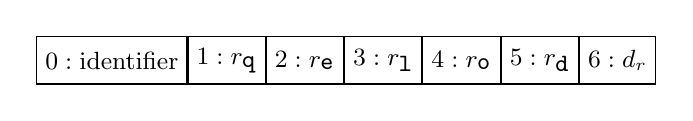
\begin{tikzpicture}
\small
\matrix[nodes={draw,minimum size=6mm}] {
  \node {$0:\textrm{identifier}$}; & \node {$1:r_\texttt{q}$}; & \node {$2:r_\texttt{e}$};
 &\node {$3:r_\texttt{l}$}; & \node {$4:r_\texttt{o}$}; & \node {$5:r_\texttt{d}$}; & \node {$6:d_r$};\\
};
\end{tikzpicture}
\end{tabular}\\
\textbf{Returns:} nothing.\\
\textbf{Side Effects:} inserts a row into each of the user tables, insert a
row into Table R, puts an entry into {\tt{}\protect\nwindexuse{lu{\char95}users}{lu:unusers}{NW27XAxz-17yXws-2}lu{\char95}users} and into {\tt{}\protect\nwindexuse{lu{\char95}rstatus}{lu:unrstatus}{NW27XAxz-17yXws-1}lu{\char95}rstatus}.\\
\textbf{Throws:} {\tt{}DuplicateUserException} if request already exists, or
{\tt{}SQLException} for other database failures.\\
\bottomrule
\end{tabular}
\nwenddocs{}\nwbegincode{83}\sublabel{NW27XAxz-4ISWm4-1}\nwmargintag{{\nwtagstyle{}\subpageref{NW27XAxz-4ISWm4-1}}}\moddef{Add new request~{\nwtagstyle{}\subpageref{NW27XAxz-4ISWm4-1}}}\endmoddef\nwalsodefined{\\{NW27XAxz-4ISWm4-2}\\{NW2ZDXo8-4ISWm4-3}}\nwused{\\{NW27XAxz-4PbjF-2}\\{NW2ZDXo8-bF3Hn-3}}
public void DBAddNewRequest(final int[] u)
throws DuplicateUserException, SQLException \{
  final int uid = u[0];
  if (this.lu_users.containsKey(uid)) \{
    throw new DuplicateUserException("User "+uid+" already exists.");
  \}
  try (\LA{}Open \code{}conn\edoc{}~{\nwtagstyle{}\subpageref{NW27XAxz-JT1v9-1}}\RA{}) \{
    try \{
      \LA{}..insert new user into user tables~{\nwtagstyle{}\subpageref{NW27XAxz-4ROa6q-1}}\RA{}
      \LA{}..insert new request into r~{\nwtagstyle{}\subpageref{NW27XAxz-44Ff7c-1}}\RA{}
      conn.commit();
    \} catch (SQLException e) \{
      conn.rollback();
      throw e;
    \}
  \} catch (SQLException e) \{
    throw e;
  \}
\nosublabel{NW27XAxz-4ISWm4-1-u3}\nwindexdefn{DBAddNewRequest}{DBAddNewRequest}{NW27XAxz-4ISWm4-1}\eatline
\nwidentdefs{\\{{DBAddNewRequest}{DBAddNewRequest}}}\nwidentuses{\\{{lu{\char95}users}{lu:unusers}}}\nwindexuse{lu{\char95}users}{lu:unusers}{NW27XAxz-4ISWm4-1}\nwendcode{}\nwbegindocs{84}{\small In the last step, we put $r$ into {\tt{}\protect\nwindexuse{lu{\char95}users}{lu:unusers}{NW27XAxz-17yXws-2}lu{\char95}users} and put it into
{\tt{}\protect\nwindexuse{lu{\char95}rstatus}{lu:unrstatus}{NW27XAxz-17yXws-1}lu{\char95}rstatus} with the value set to {\tt{}false} to indicate that it is
unassigned. When we put it into {\tt{}\protect\nwindexuse{lu{\char95}users}{lu:unusers}{NW27XAxz-17yXws-2}lu{\char95}users}, we store a cloned array {\tt{}u} as
the value because we don't want any changes to {\tt{}u} on the caller side showing
up in our cache (we are considering users to be immutable).}
\nwenddocs{}\nwbegincode{85}\sublabel{NW27XAxz-4ISWm4-2}\nwmargintag{{\nwtagstyle{}\subpageref{NW27XAxz-4ISWm4-2}}}\moddef{Add new request~{\nwtagstyle{}\subpageref{NW27XAxz-4ISWm4-1}}}\plusendmoddef
  this.lu_users.put(u[0], u.clone());
  this.lu_rstatus.put(u[0], false);
\}
\nwidentuses{\\{{lu{\char95}rstatus}{lu:unrstatus}}\\{{lu{\char95}users}{lu:unusers}}}\nwindexuse{lu{\char95}rstatus}{lu:unrstatus}{NW27XAxz-4ISWm4-2}\nwindexuse{lu{\char95}users}{lu:unusers}{NW27XAxz-4ISWm4-2}\nwendcode{}\nwbegindocs{86}\nwdocspar
{\small To insert $r$ into the user tables, we simply prepare and submit each
of the insert statements against the tables using statements {\tt{}\protect\nwindexuse{S2}{S2}{NW27XAxz-26Y6r2-1}S2} through
{\tt{}\protect\nwindexuse{S7}{S7}{NW27XAxz-3Q0zBY-1}S7}.}
\nwenddocs{}\nwbegincode{87}\sublabel{NW27XAxz-4ROa6q-1}\nwmargintag{{\nwtagstyle{}\subpageref{NW27XAxz-4ROa6q-1}}}\moddef{..insert new user into user tables~{\nwtagstyle{}\subpageref{NW27XAxz-4ROa6q-1}}}\endmoddef\nwused{\\{NW27XAxz-4ISWm4-1}\\{NW27XAxz-IYVQQ-2}}
PreparedStatement pS2 = this.PS(conn, "S2");
PreparedStatement pS3 = this.PS(conn, "S3");
PreparedStatement pS4 = this.PS(conn, "S4");
PreparedStatement pS5 = this.PS(conn, "S5");
PreparedStatement pS6 = this.PS(conn, "S6");
PreparedStatement pS7 = this.PS(conn, "S7");
this.PSAdd(pS2, uid, u[1]);
this.PSAdd(pS3, uid, u[2]);
this.PSAdd(pS4, uid, u[3]);
this.PSAdd(pS5, uid, u[4]);
this.PSAdd(pS6, uid, u[5]);
this.PSAdd(pS7, uid, u[6]);
this.PSSubmit(pS2, pS3, pS4, pS5, pS6, pS7);
\nwidentuses{\\{{PS}{PS}}\\{{PSAdd}{PSAdd}}\\{{PSSubmit}{PSSubmit}}\\{{S2}{S2}}\\{{S3}{S3}}\\{{S4}{S4}}\\{{S5}{S5}}\\{{S6}{S6}}\\{{S7}{S7}}}\nwindexuse{PS}{PS}{NW27XAxz-4ROa6q-1}\nwindexuse{PSAdd}{PSAdd}{NW27XAxz-4ROa6q-1}\nwindexuse{PSSubmit}{PSSubmit}{NW27XAxz-4ROa6q-1}\nwindexuse{S2}{S2}{NW27XAxz-4ROa6q-1}\nwindexuse{S3}{S3}{NW27XAxz-4ROa6q-1}\nwindexuse{S4}{S4}{NW27XAxz-4ROa6q-1}\nwindexuse{S5}{S5}{NW27XAxz-4ROa6q-1}\nwindexuse{S6}{S6}{NW27XAxz-4ROa6q-1}\nwindexuse{S7}{S7}{NW27XAxz-4ROa6q-1}\nwendcode{}\nwbegindocs{88}\nwdocspar
{\small Similarly, we prepare and submit statement {\tt{}\protect\nwindexuse{S9}{S9}{NW27XAxz-4Ai05A-1}S9} to insert $r$ into
Table R.}
\nwenddocs{}\nwbegincode{89}\sublabel{NW27XAxz-44Ff7c-1}\nwmargintag{{\nwtagstyle{}\subpageref{NW27XAxz-44Ff7c-1}}}\moddef{..insert new request into r~{\nwtagstyle{}\subpageref{NW27XAxz-44Ff7c-1}}}\endmoddef\nwused{\\{NW27XAxz-4ISWm4-1}}
PreparedStatement pS9 = this.PS(conn, "S9");
this.PSAdd(pS9, uid, u[1], u[2], u[3], u[4], u[5], u[6]);
this.PSSubmit(pS9);
\nwidentuses{\\{{PS}{PS}}\\{{PSAdd}{PSAdd}}\\{{PSSubmit}{PSSubmit}}\\{{S9}{S9}}}\nwindexuse{PS}{PS}{NW27XAxz-44Ff7c-1}\nwindexuse{PSAdd}{PSAdd}{NW27XAxz-44Ff7c-1}\nwindexuse{PSSubmit}{PSSubmit}{NW27XAxz-44Ff7c-1}\nwindexuse{S9}{S9}{NW27XAxz-44Ff7c-1}\nwendcode{}\nwbegindocs{90}\nwdocspar

\subsection{{\tt{}\protect\nwindexuse{DBAddNewServer}{DBAddNewServer}{NW27XAxz-IYVQQ-1}DBAddNewServer}(2)}
\begin{tabular}{p{\textwidth}}
\toprule
\rowcolor{TableTitle}
Method \textcolor{blue}{{\tt{}\protect\nwindexuse{DBAddNewServer}{DBAddNewServer}{NW27XAxz-IYVQQ-1}DBAddNewServer}}(2) inserts a new server into the
user tables and into {\tt{}\protect\nwindexuse{lu{\char95}users}{lu:unusers}{NW27XAxz-17yXws-2}lu{\char95}users} if all succeeds.  If the server attempting to
be inserted already exists, a {\tt{}DuplicateUserException} is thrown. The method
requires the server's initial route be given in the second parameter. If the
supplied route contains an edge that does not exist in Table E, an
{\tt{}EdgeNotFoundException} is thrown. A {\tt{}SQLException} is thrown for other
database failures.\\
\midrule
\textbf{Parameters:} \\
\begin{tabular}{lp{116mm}}
Array {\tt{}u} (param. 1):&7-element integer array storing values of
server $s$'s components.

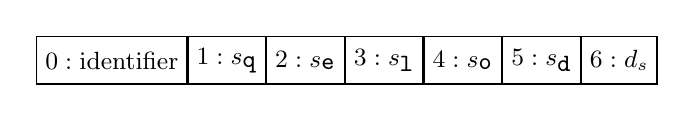
\begin{tikzpicture}
\small
\matrix[nodes={draw,minimum size=6mm}] {
  \node {$0:\textrm{identifier}$}; & \node {$1:s_\texttt{q}$}; & \node {$2:s_\texttt{e}$};
 &\node {$3:s_\texttt{l}$}; & \node {$4:s_\texttt{o}$}; & \node {$5:s_\texttt{d}$}; & \node {$6:d_s$};\\
};
\end{tikzpicture}\\
Array {\tt{}route} (param. 2):&$(2|w|)$-element integer array storing values of
waypoint components in the server's route $w$.

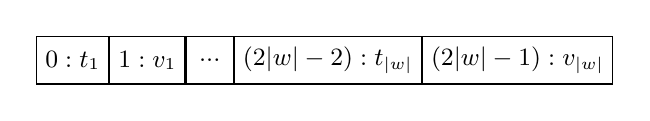
\begin{tikzpicture}
\small
\matrix[nodes={draw,minimum size=6mm}] {
  \node {$0:t_1$}; & \node {$1:v_1$}; & \node[minimum width=6mm] {...};
 &\node {$(2|w|-2):t_{|w|}$}; & \node {$(2|w|-1):v_{|w|}$}; \\
};
\end{tikzpicture}\\
\end{tabular}\\
\textbf{Returns:} nothing.\\
\textbf{Side Effects:} inserts a row into each of the user tables, insert a
row into Table S, inserts at least two rows into Table W, inserts a row into Table CW,
inserts a row into Table CQ, puts an entry into {\tt{}\protect\nwindexuse{lu{\char95}users}{lu:unusers}{NW27XAxz-17yXws-2}lu{\char95}users}.\\
\textbf{Throws:} {\tt{}DuplicateUserException} if server already exists,
{\tt{}EdgeNotFoundException} if {\tt{}route} contains an edge that does not exist
in Table E, or {\tt{}SQLException} for other database failures.\\
\bottomrule
\end{tabular}
\nwenddocs{}\nwbegincode{91}\sublabel{NW27XAxz-IYVQQ-1}\nwmargintag{{\nwtagstyle{}\subpageref{NW27XAxz-IYVQQ-1}}}\moddef{Add new server~{\nwtagstyle{}\subpageref{NW27XAxz-IYVQQ-1}}}\endmoddef\nwalsodefined{\\{NW27XAxz-IYVQQ-2}\\{NW27XAxz-IYVQQ-3}\\{NW27XAxz-IYVQQ-4}\\{NW2ZDXo8-IYVQQ-5}}\nwused{\\{NW27XAxz-4PbjF-2}\\{NW2ZDXo8-bF3Hn-3}}
public void DBAddNewServer(final int[] u, final int[] route)
throws DuplicateUserException, EdgeNotFoundException, SQLException \{
  final int uid = u[0];
  if (this.lu_users.containsKey(uid)) \{
    throw new DuplicateUserException("User "+uid+" already exists.");
  \}
  try (\LA{}Open \code{}conn\edoc{}~{\nwtagstyle{}\subpageref{NW27XAxz-JT1v9-1}}\RA{}) \{
    try \{
      final int se = u[2];
\nosublabel{NW27XAxz-IYVQQ-1-u1}\nwindexdefn{DBAddNewServer}{DBAddNewServer}{NW27XAxz-IYVQQ-1}\eatline
\nwidentdefs{\\{{DBAddNewServer}{DBAddNewServer}}}\nwidentuses{\\{{lu{\char95}users}{lu:unusers}}}\nwindexuse{lu{\char95}users}{lu:unusers}{NW27XAxz-IYVQQ-1}\nwendcode{}\nwbegindocs{92}{\small We can re-use the chunk from {\tt{}\protect\nwindexuse{DBAddNewRequest}{DBAddNewRequest}{NW27XAxz-4ISWm4-1}DBAddNewRequest}(1) to insert the
server into the user tables.}
\nwenddocs{}\nwbegincode{93}\sublabel{NW27XAxz-IYVQQ-2}\nwmargintag{{\nwtagstyle{}\subpageref{NW27XAxz-IYVQQ-2}}}\moddef{Add new server~{\nwtagstyle{}\subpageref{NW27XAxz-IYVQQ-1}}}\plusendmoddef
      \LA{}..insert new user into user tables~{\nwtagstyle{}\subpageref{NW27XAxz-4ROa6q-1}}\RA{}
\nwendcode{}\nwbegindocs{94}\nwdocspar
{\small Then we prepare and submit the insert statements that will insert $s$
into Table S and insert {\tt{}route} into Tables W and CW. Next we record the
server's initial load into Table CQ. A ``label'' marks where each chunk begins
in the source code ({\tt{}Storage.java}).}
\nwenddocs{}\nwbegincode{95}\sublabel{NW27XAxz-IYVQQ-3}\nwmargintag{{\nwtagstyle{}\subpageref{NW27XAxz-IYVQQ-3}}}\moddef{Add new server~{\nwtagstyle{}\subpageref{NW27XAxz-IYVQQ-1}}}\plusendmoddef
/*L1*/\LA{}..insert new server into s~{\nwtagstyle{}\subpageref{NW27XAxz-JGp6y-1}}\RA{}
/*L2*/\LA{}..insert new server route into w~{\nwtagstyle{}\subpageref{NW27XAxz-3xg8Fp-1}}\RA{}
/*L3*/\LA{}..insert new server route into cw~{\nwtagstyle{}\subpageref{NW27XAxz-2GDxmx-1}}\RA{}
/*L4*/\LA{}..insert new server into cq~{\nwtagstyle{}\subpageref{NW27XAxz-404DhQ-1}}\RA{}
      conn.commit();
    \} catch (SQLException e) \{
      conn.rollback();
      throw e;
    \}
  \} catch (SQLException e) \{
    throw e;
  \}
\nwendcode{}\nwbegindocs{96}\nwdocspar
{\small In the last step, we put $s$ into {\tt{}\protect\nosublabel{NW27XAxz-IYVQQ-3-u4}\protect\nwindexuse{lu{\char95}users}{lu:unusers}{NW27XAxz-17yXws-2}lu{\char95}users}.}
\nwenddocs{}\nwbegincode{97}\sublabel{NW27XAxz-IYVQQ-4}\nwmargintag{{\nwtagstyle{}\subpageref{NW27XAxz-IYVQQ-4}}}\moddef{Add new server~{\nwtagstyle{}\subpageref{NW27XAxz-IYVQQ-1}}}\plusendmoddef
  this.lu_users.put(uid, u.clone());
\}
\nwidentuses{\\{{lu{\char95}users}{lu:unusers}}}\nwindexuse{lu{\char95}users}{lu:unusers}{NW27XAxz-IYVQQ-4}\nwendcode{}\nwbegindocs{98}\nwdocspar
{\small We prepare and submit statement {\tt{}\protect\nwindexuse{S8}{S8}{NW27XAxz-PwvQG-1}S8} to insert $s$ into Table S.}
\nwenddocs{}\nwbegincode{99}\sublabel{NW27XAxz-JGp6y-1}\nwmargintag{{\nwtagstyle{}\subpageref{NW27XAxz-JGp6y-1}}}\moddef{..insert new server into s~{\nwtagstyle{}\subpageref{NW27XAxz-JGp6y-1}}}\endmoddef\nwused{\\{NW27XAxz-IYVQQ-3}}
PreparedStatement pS8 = this.PS(conn, "S8");
this.PSAdd(pS8, uid, u[1], u[2], u[3], u[4], u[5], u[6]);
this.PSSubmit(pS8);
\nwidentuses{\\{{PS}{PS}}\\{{PSAdd}{PSAdd}}\\{{PSSubmit}{PSSubmit}}\\{{S8}{S8}}}\nwindexuse{PS}{PS}{NW27XAxz-JGp6y-1}\nwindexuse{PSAdd}{PSAdd}{NW27XAxz-JGp6y-1}\nwindexuse{PSSubmit}{PSSubmit}{NW27XAxz-JGp6y-1}\nwindexuse{S8}{S8}{NW27XAxz-JGp6y-1}\nwendcode{}\nwbegindocs{100}\nwdocspar
{\small The procedure to insert {\tt{}route} into Table W is written into its own
chunk so we can re-use it later.  After the procedure, we re-initialize
statement {\tt{}\protect\nwindexuse{S10}{S10}{NW27XAxz-96fbA-1}S10} to add the first waypoint $(t_1,v_1)$ into columns
\textsf{t2} and \textsf{v2} while setting columns \textsf{t1} and \textsf{v1}
to {\tt{}null}.}
\nwenddocs{}\nwbegincode{101}\sublabel{NW27XAxz-3xg8Fp-1}\nwmargintag{{\nwtagstyle{}\subpageref{NW27XAxz-3xg8Fp-1}}}\moddef{..insert new server route into w~{\nwtagstyle{}\subpageref{NW27XAxz-3xg8Fp-1}}}\endmoddef\nwused{\\{NW27XAxz-IYVQQ-3}}
\LA{}Procedure to insert \code{}route\edoc{} into Table W~{\nwtagstyle{}\subpageref{NW27XAxz-1EP7t-1}}\RA{}
pS10 = this.PS(conn, "S10");
this.PSAdd(pS10, uid, se, null, null, route[0], route[1], null, null);
this.PSSubmit(pS10);
\nwidentuses{\\{{PS}{PS}}\\{{PSAdd}{PSAdd}}\\{{PSSubmit}{PSSubmit}}\\{{S10}{S10}}}\nwindexuse{PS}{PS}{NW27XAxz-3xg8Fp-1}\nwindexuse{PSAdd}{PSAdd}{NW27XAxz-3xg8Fp-1}\nwindexuse{PSSubmit}{PSSubmit}{NW27XAxz-3xg8Fp-1}\nwindexuse{S10}{S10}{NW27XAxz-3xg8Fp-1}\nwendcode{}\nwbegindocs{102}\nwdocspar
{\small In the procedure to insert {\tt{}route} into Table W, we loop through each
of the waypoints, adding the waypoint $(t_i,v_i)$ into columns \textsf{t1} and
\textsf{v1} and adding its successor $(t_{i+1},v_{i+1})$ into columns
\textsf{t2} and \textsf{v2}. We start by treating $(t_1,v_1)$ as the
predecessor for $(t_2,v_2)$, then add the predecessor to $(t_1,v_1)$ seperately
as mentioned above.}
\nwenddocs{}\nwbegincode{103}\sublabel{NW27XAxz-1EP7t-1}\nwmargintag{{\nwtagstyle{}\subpageref{NW27XAxz-1EP7t-1}}}\moddef{Procedure to insert \code{}route\edoc{} into Table W~{\nwtagstyle{}\subpageref{NW27XAxz-1EP7t-1}}}\endmoddef\nwused{\\{NW27XAxz-3xg8Fp-1}\\{NW27XAxz-2BaQBV-1}}
PreparedStatement pS10 = this.PS(conn, "S10");
for (int i = 0; i < (route.length - 3); i += 2) \{
  final int t1 = route[(i + 0)];
  final int v1 = route[(i + 1)];
  final int t2 = route[(i + 2)];
  final int v2 = route[(i + 3)];
  if (!(this.lu_edges.containsKey(v1) && this.lu_edges.get(v1).containsKey(v2))) \{
    throw new EdgeNotFoundException("Edge ("+v1+", "+v2+") not found.");
  \}
  final int dd = this.lu_edges.get(v1).get(v2)[0];
  final int nu = this.lu_edges.get(v1).get(v2)[1];
  this.PSAdd(pS10, uid, se, t1, v1, t2, v2, dd, nu);
\}
this.PSSubmit(pS10);
\nwidentuses{\\{{lu{\char95}edges}{lu:unedges}}\\{{PS}{PS}}\\{{PSAdd}{PSAdd}}\\{{PSSubmit}{PSSubmit}}\\{{S10}{S10}}}\nwindexuse{lu{\char95}edges}{lu:unedges}{NW27XAxz-1EP7t-1}\nwindexuse{PS}{PS}{NW27XAxz-1EP7t-1}\nwindexuse{PSAdd}{PSAdd}{NW27XAxz-1EP7t-1}\nwindexuse{PSSubmit}{PSSubmit}{NW27XAxz-1EP7t-1}\nwindexuse{S10}{S10}{NW27XAxz-1EP7t-1}\nwendcode{}\nwbegindocs{104}\nwdocspar
{\small We prepare and submit statement {\tt{}\protect\nwindexuse{S11}{S11}{NW27XAxz-4dHZ4O-1}S11} to insert the server's
start and end times into Table CW.}
\nwenddocs{}\nwbegincode{105}\sublabel{NW27XAxz-2GDxmx-1}\nwmargintag{{\nwtagstyle{}\subpageref{NW27XAxz-2GDxmx-1}}}\moddef{..insert new server route into cw~{\nwtagstyle{}\subpageref{NW27XAxz-2GDxmx-1}}}\endmoddef\nwused{\\{NW27XAxz-IYVQQ-3}}
PreparedStatement pS11 = this.PS(conn, "S11");
final int te = route[(route.length - 2)];
this.PSAdd(pS11, uid, u[2], u[3], u[4], u[5], u[2], u[4], te, u[5]);
this.PSSubmit(pS11);
\nwidentuses{\\{{PS}{PS}}\\{{PSAdd}{PSAdd}}\\{{PSSubmit}{PSSubmit}}\\{{S11}{S11}}}\nwindexuse{PS}{PS}{NW27XAxz-2GDxmx-1}\nwindexuse{PSAdd}{PSAdd}{NW27XAxz-2GDxmx-1}\nwindexuse{PSSubmit}{PSSubmit}{NW27XAxz-2GDxmx-1}\nwindexuse{S11}{S11}{NW27XAxz-2GDxmx-1}\nwendcode{}\nwbegindocs{106}\nwdocspar
{\small We prepare and submit statement {\tt{}\protect\nwindexuse{S14}{S14}{NW27XAxz-yU48q-1}S14} to insert the server's
initial load into Table CQ.}
\nwenddocs{}\nwbegincode{107}\sublabel{NW27XAxz-404DhQ-1}\nwmargintag{{\nwtagstyle{}\subpageref{NW27XAxz-404DhQ-1}}}\moddef{..insert new server into cq~{\nwtagstyle{}\subpageref{NW27XAxz-404DhQ-1}}}\endmoddef\nwused{\\{NW27XAxz-IYVQQ-3}}
PreparedStatement pS14 = this.PS(conn, "S14");
this.PSAdd(pS14, uid, u[1], u[2], null, u[2], u[4], null, u[1],
    null, null, null, null, null, 1);
this.PSSubmit(pS14);
\nwidentuses{\\{{PS}{PS}}\\{{PSAdd}{PSAdd}}\\{{PSSubmit}{PSSubmit}}\\{{S14}{S14}}}\nwindexuse{PS}{PS}{NW27XAxz-404DhQ-1}\nwindexuse{PSAdd}{PSAdd}{NW27XAxz-404DhQ-1}\nwindexuse{PSSubmit}{PSSubmit}{NW27XAxz-404DhQ-1}\nwindexuse{S14}{S14}{NW27XAxz-404DhQ-1}\nwendcode{}\nwbegindocs{108}\nwdocspar

\subsection{{\tt{}\protect\nwindexuse{DBUpdateServerRoute}{DBUpdateServerRoute}{NW27XAxz-4VFddh-1}DBUpdateServerRoute}(3)}
\begin{tabular}{p{\textwidth}}
\toprule
\rowcolor{TableTitle}
Method \textcolor{blue}{{\tt{}\protect\nwindexuse{DBUpdateServerRoute}{DBUpdateServerRoute}{NW27XAxz-4VFddh-1}DBUpdateServerRoute}}(3) inserts a new
\emph{remaining route} for server $s$ into Table W. As the timing of waypoints
may change, the method also updates timings in the \emph{remaining schedule}.
If the server to be updated does not exist, a {\tt{}UserNotFoundException} is
thrown.  If the supplied route contains an edge that does not exist in Table E,
an {\tt{}EdgeNotFoundException} is thrown. A {\tt{}SQLException} is thrown for other
database failures.\\
\midrule
\textbf{Parameters:} \\
\begin{tabular}{lp{116mm}}
Integer {\tt{}sid} (param. 1):&server identifier.\\
Array {\tt{}route} (param. 2):&$2n$-element integer array storing values of
waypoint components in the server's $n$-length remaining route $w_{>t}$.
In the diagram, $|w|-i=n$.
Here $t$ is taken to be {\tt{}route[0]}. Consequently, $(t_i,v_i)$ is \emph{not} part
of the remaining route, in other words \textbf{it must pre-exist in Table W}.

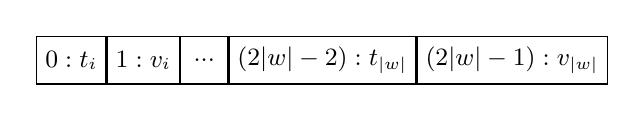
\begin{tikzpicture}
\small
\matrix[nodes={draw,minimum size=6mm}] {
  \node {$0:t_i$}; & \node {$1:v_i$}; & \node[minimum width=6mm] {...};
 &\node {$(2|w|-2):t_{|w|}$}; & \node {$(2|w|-1):v_{|w|}$}; \\
};
\end{tikzpicture}\\
Array {\tt{}sched} (param. 2):&$3m$-element integer array storing values of
waypoint components and their labels in the server's $m$-length remaining
schedule $b_{>t}$, where $m\leq n$. In the diagram, $|b|-j=m$.  Note
$(t_{i_j},v_{i_j})$ \emph{cannot equal} $(t_i,v_i)$, as $(t_i,v_i)$ is part of
the traveled route and not the remaining route (we cannot change the past).
Therefore $t_{i_j}$ \textbf{must be greater than} $t_i$. Due to rule R3,
$(t_{i_{|b|}},v_{i_{|b|}})$ \textbf{must equal} $(t_{|w|},v_{|w|})$.

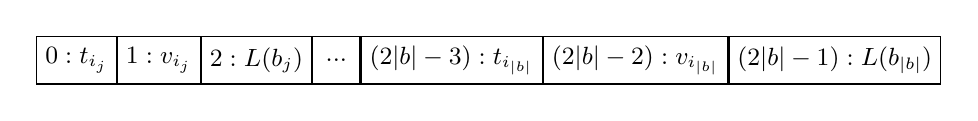
\begin{tikzpicture}
\small
\matrix[nodes={draw,minimum size=6mm}] {
  \node {$0:t_{i_j}$}; & \node {$1:v_{i_j}$}; & \node {$2:L(b_j)$}; & \node[minimum width=6mm] {...};
 &\node {$(2|b|-3):t_{i_{|b|}}$}; & \node {$(2|b|-2):v_{i_{|b|}}$}; & \node {$(2|b|-1):L(b_{|b|})$};\\
};
\end{tikzpicture}

If a waypoint has multiple labels, write them side-by-side, \textit{e.g.}
to record two labels $L_1(b_j)$ and $L_2(b_j)$ on waypoint $b_j$, write
(indices omitted for clarity):

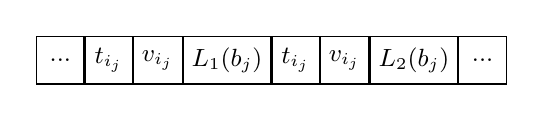
\begin{tikzpicture}
\small
\matrix[nodes={draw,minimum size=6mm}] {
  \node[minimum width=6mm] {...};
 &\node {$t_{i_j}$}; & \node {$v_{i_j}$};
 &\node {$L_1(b_j)$};
 &\node {$t_{i_j}$}; & \node {$v_{i_j}$};
 &\node {$L_2(b_j)$};
 &\node[minimum width=6mm] {...};\\
};
\end{tikzpicture}

If a waypoint has multiple labels with some indicating drop-offs, \textbf{write
the drop-offs first} before any of the pick-ups, otherwise C98 violation may
occur.
\end{tabular}\\
\textbf{Returns:} nothing.\\
\textbf{Side Effects:} may delete and insert rows into Table W, may
update columns in Table CW, may update columns in Tables PD and CPD,
may delete and insert rows into Table CQ.\\
\textbf{Throws:} {\tt{}UserNotFoundException} if server does not exist,
{\tt{}EdgeNotFoundException} if {\tt{}route} contains an edge that does not exist
in Table E, or {\tt{}SQLException} for other database failures.\\
\bottomrule
\end{tabular}
\nwenddocs{}\nwbegincode{109}\sublabel{NW27XAxz-4VFddh-1}\nwmargintag{{\nwtagstyle{}\subpageref{NW27XAxz-4VFddh-1}}}\moddef{Update server route~{\nwtagstyle{}\subpageref{NW27XAxz-4VFddh-1}}}\endmoddef\nwalsodefined{\\{NWvbkzY-4VFddh-2}}\nwused{\\{NW27XAxz-4PbjF-2}\\{NWvbkzY-3YjONp-2}}
public void DBUpdateServerRoute(final int sid, final int[] route, final int[] sched)
throws UserNotFoundException, EdgeNotFoundException, SQLException \{
  if (!this.lu_users.containsKey(sid)) \{
    throw new UserNotFoundException("User "+sid+" not found.");
  \}
  try (\LA{}Open \code{}conn\edoc{}~{\nwtagstyle{}\subpageref{NW27XAxz-JT1v9-1}}\RA{}) \{
    try \{
/*L1*/\LA{}..fetch \code{}sq\edoc{} and \code{}se\edoc{}~{\nwtagstyle{}\subpageref{NW27XAxz-2VNDCH-1}}\RA{}
/*L2*/\LA{}..update route~{\nwtagstyle{}\subpageref{NW27XAxz-4LV9nl-1}}\RA{}
      if (sched.length > 0) \{
        Map<Integer, int[]> cache = new HashMap<>();
/*L3*/  \LA{}..update schedule~{\nwtagstyle{}\subpageref{NW27XAxz-2NqWTJ-1}}\RA{}
      \}
      conn.commit();
    \} catch (SQLException e) \{
      conn.rollback();
      throw e;
    \}
  \} catch (SQLException e) \{
    throw e;
  \}
\}
\nosublabel{NW27XAxz-4VFddh-1-u4}\nwindexdefn{DBUpdateServerRoute}{DBUpdateServerRoute}{NW27XAxz-4VFddh-1}\eatline
\nwidentdefs{\\{{DBUpdateServerRoute}{DBUpdateServerRoute}}}\nwidentuses{\\{{lu{\char95}users}{lu:unusers}}}\nwindexuse{lu{\char95}users}{lu:unusers}{NW27XAxz-4VFddh-1}\nwendcode{}\nwbegindocs{110}{\small We get the server's load into {\tt{}sq}, needed by Table CQ. We also
get the server's early time into {\tt{}se}, needed by the procedure to insert
{\tt{}route} into Table W.}
\nwenddocs{}\nwbegincode{111}\sublabel{NW27XAxz-2VNDCH-1}\nwmargintag{{\nwtagstyle{}\subpageref{NW27XAxz-2VNDCH-1}}}\moddef{..fetch \code{}sq\edoc{} and \code{}se\edoc{}~{\nwtagstyle{}\subpageref{NW27XAxz-2VNDCH-1}}}\endmoddef\nwused{\\{NW27XAxz-4VFddh-1}\\{NW27XAxz-y828a-1}\\{NW27XAxz-lMiTm-1}}
final int sq = lu_users.get(sid)[1];
final int se = lu_users.get(sid)[2];
\nwidentuses{\\{{lu{\char95}users}{lu:unusers}}}\nwindexuse{lu{\char95}users}{lu:unusers}{NW27XAxz-2VNDCH-1}\nwendcode{}\nwbegindocs{112}\nwdocspar
{\small To update the route, first we delete the pre-existing remaining route
from Table W, then insert the waypoints in {\tt{}route}, and lastly update the
route endpoint in Table CW. As Table CPD stores the route endpoint time in
column \textsf{te}, we update this table as well.}
\nwenddocs{}\nwbegincode{113}\sublabel{NW27XAxz-4LV9nl-1}\nwmargintag{{\nwtagstyle{}\subpageref{NW27XAxz-4LV9nl-1}}}\moddef{..update route~{\nwtagstyle{}\subpageref{NW27XAxz-4LV9nl-1}}}\endmoddef\nwused{\\{NW27XAxz-4VFddh-1}\\{NW27XAxz-y828a-1}\\{NW27XAxz-lMiTm-1}}
/*a*/\LA{}....delete remaining route from w~{\nwtagstyle{}\subpageref{NW27XAxz-1n0DBP-1}}\RA{}
/*b*/\LA{}....insert new remaining route into w~{\nwtagstyle{}\subpageref{NW27XAxz-2BaQBV-1}}\RA{}
/*c*/\LA{}....update route endpoint in cw, cpd~{\nwtagstyle{}\subpageref{NW27XAxz-1ZiLuE-1}}\RA{}
\nwendcode{}\nwbegindocs{114}\nwdocspar
{\small We prepare and submit statement {\tt{}\protect\nosublabel{NW27XAxz-4LV9nl-1-u3}\protect\nwindexuse{S76}{S76}{NW27XAxz-1SHBum-1}S76} to delete the pre-existing
remaining route from Table W.}
\nwenddocs{}\nwbegincode{115}\sublabel{NW27XAxz-1n0DBP-1}\nwmargintag{{\nwtagstyle{}\subpageref{NW27XAxz-1n0DBP-1}}}\moddef{....delete remaining route from w~{\nwtagstyle{}\subpageref{NW27XAxz-1n0DBP-1}}}\endmoddef\nwused{\\{NW27XAxz-4LV9nl-1}}
PreparedStatement pS76 = this.PS(conn, "S76");
this.PSAdd(pS76, sid, route[0]);
this.PSSubmit(pS76);
\nwidentuses{\\{{PS}{PS}}\\{{PSAdd}{PSAdd}}\\{{PSSubmit}{PSSubmit}}\\{{S76}{S76}}}\nwindexuse{PS}{PS}{NW27XAxz-1n0DBP-1}\nwindexuse{PSAdd}{PSAdd}{NW27XAxz-1n0DBP-1}\nwindexuse{PSSubmit}{PSSubmit}{NW27XAxz-1n0DBP-1}\nwindexuse{S76}{S76}{NW27XAxz-1n0DBP-1}\nwendcode{}\nwbegindocs{116}\nwdocspar
{\small We re-use the chunk that inserts {\tt{}route} into Table W.}
\nwenddocs{}\nwbegincode{117}\sublabel{NW27XAxz-2BaQBV-1}\nwmargintag{{\nwtagstyle{}\subpageref{NW27XAxz-2BaQBV-1}}}\moddef{....insert new remaining route into w~{\nwtagstyle{}\subpageref{NW27XAxz-2BaQBV-1}}}\endmoddef\nwused{\\{NW27XAxz-4LV9nl-1}}
final int uid = sid;
\LA{}Procedure to insert \code{}route\edoc{} into Table W~{\nwtagstyle{}\subpageref{NW27XAxz-1EP7t-1}}\RA{}
\nwendcode{}\nwbegindocs{118}\nwdocspar
{\small We prepare and submit statements {\tt{}\protect\nosublabel{NW27XAxz-2BaQBV-1-u1}\protect\nwindexuse{S77}{S77}{NW27XAxz-3PlVaO-1}S77} and {\tt{}\protect\nwindexuse{S139}{S139}{NW27XAxz-44lfAZ-1}S139} to update the
route endpoint in Tables CW and CPD.}
\nwenddocs{}\nwbegincode{119}\sublabel{NW27XAxz-1ZiLuE-1}\nwmargintag{{\nwtagstyle{}\subpageref{NW27XAxz-1ZiLuE-1}}}\moddef{....update route endpoint in cw, cpd~{\nwtagstyle{}\subpageref{NW27XAxz-1ZiLuE-1}}}\endmoddef\nwused{\\{NW27XAxz-4LV9nl-1}}
PreparedStatement pS77 = this.PS(conn, "S77");
PreparedStatement pS139 = this.PS(conn, "S139");
final int te = sched[(sched.length - 3)];
final int ve = sched[(sched.length - 2)];
this.PSAdd(pS77, te, ve, sid);
this.PSAdd(pS139, te, sid);
this.PSSubmit(pS77, pS139);
\nwidentuses{\\{{PS}{PS}}\\{{PSAdd}{PSAdd}}\\{{PSSubmit}{PSSubmit}}\\{{S139}{S139}}\\{{S77}{S77}}}\nwindexuse{PS}{PS}{NW27XAxz-1ZiLuE-1}\nwindexuse{PSAdd}{PSAdd}{NW27XAxz-1ZiLuE-1}\nwindexuse{PSSubmit}{PSSubmit}{NW27XAxz-1ZiLuE-1}\nwindexuse{S139}{S139}{NW27XAxz-1ZiLuE-1}\nwindexuse{S77}{S77}{NW27XAxz-1ZiLuE-1}\nwendcode{}\nwbegindocs{120}\nwdocspar
{\small To update the schedule, first we update the time values in column
\textsf{t2} of Table PD and in columns \textsf{tp} and \textsf{td} of Table
CPD. Then we prepare to update Table CQ. The method does not require
pick-ups and drop-offs in {\tt{}sched} be in the same order as in the pre-existing
remaining schedule. Consequently simply updating column \textsf{t2} in Table CQ
is not enough. Our approach here follows our approach for
updating the route. That is, first we delete the pre-existing remaining
schedule, and then we insert the waypoints in {\tt{}sched}. In order to do so, we
need to know the pick-up and drop-off times of every request in the remaining
schedule, as required by constraints F46 and F47. We also need to know the
latest order number so we can fill in columns \textsf{o1} and \textsf{o2}. Thus
we perform some queries to get the required values before finally submitting
the individual insert statements.}
\nwenddocs{}\nwbegincode{121}\sublabel{NW27XAxz-2NqWTJ-1}\nwmargintag{{\nwtagstyle{}\subpageref{NW27XAxz-2NqWTJ-1}}}\moddef{..update schedule~{\nwtagstyle{}\subpageref{NW27XAxz-2NqWTJ-1}}}\endmoddef\nwalsodefined{\\{NW27XAxz-2NqWTJ-2}}\nwused{\\{NW27XAxz-4VFddh-1}\\{NW27XAxz-lMiTm-1}}
/*a*/\LA{}....update times in pd and cpd~{\nwtagstyle{}\subpageref{NW27XAxz-1cwA5Z-1}}\RA{}
\nwendcode{}\nwbegindocs{122}{\small Here begins the procedure to update Table CQ.}
\nwenddocs{}\nwbegincode{123}\sublabel{NW27XAxz-2NqWTJ-2}\nwmargintag{{\nwtagstyle{}\subpageref{NW27XAxz-2NqWTJ-2}}}\moddef{..update schedule~{\nwtagstyle{}\subpageref{NW27XAxz-2NqWTJ-1}}}\plusendmoddef
/*b*/\LA{}....populate the tp, td cache and update cq~{\nwtagstyle{}\subpageref{NW27XAxz-1OV3dP-1}}\RA{}
/*c*/\LA{}....select latest order number~{\nwtagstyle{}\subpageref{NW27XAxz-1gWfDY-1}}\RA{}
/*d*/\LA{}....delete remaining schedule from cq~{\nwtagstyle{}\subpageref{NW27XAxz-4AIXfi-1}}\RA{}
/*e*/\LA{}....insert new remaining schedule into cq~{\nwtagstyle{}\subpageref{NW27XAxz-2Ir9Yx-1}}\RA{}
\nwendcode{}\nwbegindocs{124}\nwdocspar
{\small We prepare and submit statements {\tt{}\protect\nosublabel{NW27XAxz-2NqWTJ-2-u4}\protect\nwindexuse{S82}{S82}{NW27XAxz-25vZHI-1}S82}, {\tt{}\protect\nwindexuse{S83}{S83}{NW27XAxz-2TlsCi-1}S83}, and {\tt{}\protect\nwindexuse{S84}{S84}{NW27XAxz-yx2fc-1}S84} to
update the times in Tables PD and CPD. As we don't know at this point if a
waypoint in {\tt{}sched} represents a pick-up or a drop-off, we issue both
{\tt{}\protect\nwindexuse{S82}{S82}{NW27XAxz-25vZHI-1}S82}, updating pick-up time \textsf{tp}, and {\tt{}\protect\nwindexuse{S83}{S83}{NW27XAxz-2TlsCi-1}S83}, updating drop-off time
\textsf{td}, for all waypoints. As desired, only one of these statements will
succeed due to the {\tt{}WHERE} conditions in the statements.}
\nwenddocs{}\nwbegincode{125}\sublabel{NW27XAxz-1cwA5Z-1}\nwmargintag{{\nwtagstyle{}\subpageref{NW27XAxz-1cwA5Z-1}}}\moddef{....update times in pd and cpd~{\nwtagstyle{}\subpageref{NW27XAxz-1cwA5Z-1}}}\endmoddef\nwused{\\{NW27XAxz-2NqWTJ-1}\\{NW27XAxz-2VQLMF-1}}
PreparedStatement pS82 = this.PS(conn, "S82");
PreparedStatement pS83 = this.PS(conn, "S83");
PreparedStatement pS84 = this.PS(conn, "S84");
for (int j = 0; j < (sched.length - 2); j += 3) \{
  final int tj = sched[(j + 0)];
  final int vj = sched[(j + 1)];
  final int Lj = sched[(j + 2)];
  if (Lj != sid) \{
    this.PSAdd(pS82, tj, vj, Lj);
    this.PSAdd(pS83, tj, vj, Lj);
    this.PSAdd(pS84, tj, vj, Lj);
  \}
\}
this.PSSubmit(pS82, pS83, pS84);
\nwidentuses{\\{{PS}{PS}}\\{{PSAdd}{PSAdd}}\\{{PSSubmit}{PSSubmit}}\\{{S82}{S82}}\\{{S83}{S83}}\\{{S84}{S84}}}\nwindexuse{PS}{PS}{NW27XAxz-1cwA5Z-1}\nwindexuse{PSAdd}{PSAdd}{NW27XAxz-1cwA5Z-1}\nwindexuse{PSSubmit}{PSSubmit}{NW27XAxz-1cwA5Z-1}\nwindexuse{S82}{S82}{NW27XAxz-1cwA5Z-1}\nwindexuse{S83}{S83}{NW27XAxz-1cwA5Z-1}\nwindexuse{S84}{S84}{NW27XAxz-1cwA5Z-1}\nwendcode{}\nwbegindocs{126}\nwdocspar
{\small To insert a load change due to pick-up or drop-off of a request into
Table CQ, we are required to know the time of both the pick-up and the drop-off
of the request. In this chunk, we loop through all the requests in {\tt{}sched}
and use statement {\tt{}\protect\nwindexuse{S86}{S86}{NW27XAxz-1Ru7wC-1}S86} to get the request's pick-up and drop-off times from
the newly-updated Table CPD. We store the obtained times, along with the
request's load, into a temporary map called {\tt{}cache}. At the same time, we go
ahead and use statement {\tt{}\protect\nwindexuse{S140}{S140}{NW27XAxz-yno67-1}S140} to update Table CQ with the discovered pick-up
and drop-off times.}
\nwenddocs{}\nwbegincode{127}\sublabel{NW27XAxz-1OV3dP-1}\nwmargintag{{\nwtagstyle{}\subpageref{NW27XAxz-1OV3dP-1}}}\moddef{....populate the tp, td cache and update cq~{\nwtagstyle{}\subpageref{NW27XAxz-1OV3dP-1}}}\endmoddef\nwused{\\{NW27XAxz-2NqWTJ-2}}
PreparedStatement pS140 = this.PS(conn, "S140");
for (int j = 0; j < (sched.length - 2); j += 3) \{
  final int Lj = sched[(j + 2)];
  if (Lj != sid) \{
    if (!cache.containsKey(Lj)) \{
      final int[] output = DBFetch(conn, "S86", 2, Lj);
      final int tp = output[0];
      final int td = output[1];
      final int rq = this.lu_users.get(Lj)[1];
      cache.put(Lj, new int[] \{ rq, tp, td \});
      this.PSAdd(pS140, tp, td, Lj);
    \}
  \}
\}
this.PSSubmit(pS140);
\nwidentuses{\\{{DBFetch}{DBFetch}}\\{{lu{\char95}users}{lu:unusers}}\\{{PS}{PS}}\\{{PSAdd}{PSAdd}}\\{{PSSubmit}{PSSubmit}}\\{{S140}{S140}}\\{{S86}{S86}}}\nwindexuse{DBFetch}{DBFetch}{NW27XAxz-1OV3dP-1}\nwindexuse{lu{\char95}users}{lu:unusers}{NW27XAxz-1OV3dP-1}\nwindexuse{PS}{PS}{NW27XAxz-1OV3dP-1}\nwindexuse{PSAdd}{PSAdd}{NW27XAxz-1OV3dP-1}\nwindexuse{PSSubmit}{PSSubmit}{NW27XAxz-1OV3dP-1}\nwindexuse{S140}{S140}{NW27XAxz-1OV3dP-1}\nwindexuse{S86}{S86}{NW27XAxz-1OV3dP-1}\nwendcode{}\nwbegindocs{128}\nwdocspar
{\small We are also required to know the latest order number so we can
correctly set columns \textsf{o1} and \textsf{o2}. We use statement {\tt{}\protect\nwindexuse{S87}{S87}{NW27XAxz-3PORbo-1}S87} to
obtain this value and other values from the preceding order. For the special
case where $t=0$, we can skip the query.}
\nwenddocs{}\nwbegincode{129}\sublabel{NW27XAxz-1gWfDY-1}\nwmargintag{{\nwtagstyle{}\subpageref{NW27XAxz-1gWfDY-1}}}\moddef{....select latest order number~{\nwtagstyle{}\subpageref{NW27XAxz-1gWfDY-1}}}\endmoddef\nwused{\\{NW27XAxz-2NqWTJ-2}\\{NW27XAxz-2VQLMF-1}}
final int[] output = (route[0] == 0 ? null : this.DBFetch(conn, "S87", 3, sid, route[0]));
int t1 = (route[0] == 0 ?  0 : output[0]);
int q1 = (route[0] == 0 ? sq : output[1]);
int o1 = (route[0] == 0 ?  1 : output[2]);
\nwidentuses{\\{{DBFetch}{DBFetch}}\\{{S87}{S87}}}\nwindexuse{DBFetch}{DBFetch}{NW27XAxz-1gWfDY-1}\nwindexuse{S87}{S87}{NW27XAxz-1gWfDY-1}\nwendcode{}\nwbegindocs{130}\nwdocspar
{\small We prepare and submit statement {\tt{}\protect\nwindexuse{S80}{S80}{NW27XAxz-A8qO4-1}S80} to delete the pre-existing
remaining schedule from Table CQ.}
\nwenddocs{}\nwbegincode{131}\sublabel{NW27XAxz-4AIXfi-1}\nwmargintag{{\nwtagstyle{}\subpageref{NW27XAxz-4AIXfi-1}}}\moddef{....delete remaining schedule from cq~{\nwtagstyle{}\subpageref{NW27XAxz-4AIXfi-1}}}\endmoddef\nwused{\\{NW27XAxz-2NqWTJ-2}\\{NW27XAxz-2VQLMF-1}}
PreparedStatement pS80 = this.PS(conn, "S80");
this.PSAdd(pS80, sid, route[0]);
this.PSSubmit(pS80);
\nwidentuses{\\{{PS}{PS}}\\{{PSAdd}{PSAdd}}\\{{PSSubmit}{PSSubmit}}\\{{S80}{S80}}}\nwindexuse{PS}{PS}{NW27XAxz-4AIXfi-1}\nwindexuse{PSAdd}{PSAdd}{NW27XAxz-4AIXfi-1}\nwindexuse{PSSubmit}{PSSubmit}{NW27XAxz-4AIXfi-1}\nwindexuse{S80}{S80}{NW27XAxz-4AIXfi-1}\nwendcode{}\nwbegindocs{132}\nwdocspar
{\small We prepare and submit statement {\tt{}\protect\nwindexuse{S14}{S14}{NW27XAxz-yU48q-1}S14} to insert the new remaining
schedule into Table CQ, using the pick-up and drop-off times collected in
{\tt{}cache}.}
\nwenddocs{}\nwbegincode{133}\sublabel{NW27XAxz-2Ir9Yx-1}\nwmargintag{{\nwtagstyle{}\subpageref{NW27XAxz-2Ir9Yx-1}}}\moddef{....insert new remaining schedule into cq~{\nwtagstyle{}\subpageref{NW27XAxz-2Ir9Yx-1}}}\endmoddef\nwused{\\{NW27XAxz-2NqWTJ-2}\\{NW27XAxz-2VQLMF-1}}
PreparedStatement pS14 = PS(conn, "S14");
for (int j = 0; j < (sched.length - 2); j += 3) \{
  final int t2 = sched[(j + 0)];
  final int v2 = sched[(j + 1)];
  final int Lj = sched[(j + 2)];
  if (Lj != sid) \{
    final int[] qpd = cache.get(Lj);
    final int q2 = (t2 == qpd[1] ? q1 + qpd[0] : q1 - qpd[0]);
    final int o2 = o1 + 1;
    this.PSAdd(pS14, sid, sq, se, t1, t2, v2, q1, q2, Lj,
          qpd[0], qpd[1], qpd[2], o1, o2);
    t1 = t2;
    q1 = q2;
    o1 = o2;
  \}
\}
this.PSSubmit(pS14);
\nwidentuses{\\{{PS}{PS}}\\{{PSAdd}{PSAdd}}\\{{PSSubmit}{PSSubmit}}\\{{S14}{S14}}}\nwindexuse{PS}{PS}{NW27XAxz-2Ir9Yx-1}\nwindexuse{PSAdd}{PSAdd}{NW27XAxz-2Ir9Yx-1}\nwindexuse{PSSubmit}{PSSubmit}{NW27XAxz-2Ir9Yx-1}\nwindexuse{S14}{S14}{NW27XAxz-2Ir9Yx-1}\nwendcode{}\nwbegindocs{134}\nwdocspar

\subsection{{\tt{}\protect\nwindexuse{DBUpdateServerAddToSchedule}{DBUpdateServerAddToSchedule}{NW27XAxz-y828a-1}DBUpdateServerAddToSchedule}(4)}
\begin{tabular}{p{\textwidth}}
\toprule
\rowcolor{TableTitle}
Method \textcolor{blue}{{\tt{}\protect\nwindexuse{DBUpdateServerAddToSchedule}{DBUpdateServerAddToSchedule}{NW27XAxz-y828a-1}DBUpdateServerAddToSchedule}}(4) inserts a new
\emph{remaining route} for server $s$ into Table W, and a new \emph{remaining
schedule} with \emph{new labeled waypoints} not found in the pre-existing
remaining schedule into Tables PD, CPD, and CQ.  If the server to be updated
does not exist, a {\tt{}UserNotFoundException} is thrown.  This exception is also
thrown if any labels in the new labeled waypoints is not an existing user.  If
the supplied route contains an edge that does not exist in Table E, an
{\tt{}EdgeNotFoundException} is thrown.  A {\tt{}SQLException} is thrown for other
database failures.\\
\midrule
\textbf{Parameters:} \\
\begin{tabular}{lp{116mm}}
Integer {\tt{}sid} (param. 1):&server identifier.\\
Array {\tt{}route} (param. 2):&$2n$-element integer array storing values of
waypoint components in the server's $n$-length remaining route $w_{>t}$.
In the diagram, $|w|-i=n$.
Here $t$ is taken to be {\tt{}route[0]}. Consequently, $(t_i,v_i)$ is \emph{not} part
of the remaining route, in other words \textbf{it must pre-exist in Table W}.

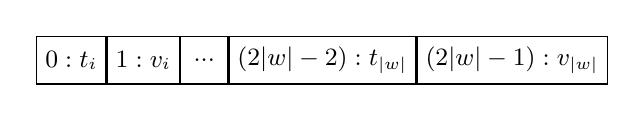
\begin{tikzpicture}
\small
\matrix[nodes={draw,minimum size=6mm}] {
  \node {$0:t_i$}; & \node {$1:v_i$}; & \node[minimum width=6mm] {...};
 &\node {$(2|w|-2):t_{|w|}$}; & \node {$(2|w|-1):v_{|w|}$}; \\
};
\end{tikzpicture}\\
Array {\tt{}sched} (param. 2):&$3m$-element integer array storing values of
waypoint components and their labels in the server's $m$-length remaining
schedule $b_{>t}$, where $m\leq n$. In the diagram, $|b|-j=m$.  Note
$(t_{i_j},v_{i_j})$ \emph{cannot equal} $(t_i,v_i)$, as $(t_i,v_i)$ is part of
the traveled route and not the remaining route (we cannot change the past).
Therefore $t_{i_j}$ \textbf{must be greater than} $t_i$. Due to rule R3,
$(t_{i_{|b|}},v_{i_{|b|}})$ \textbf{must equal} $(t_{|w|},v_{|w|})$.

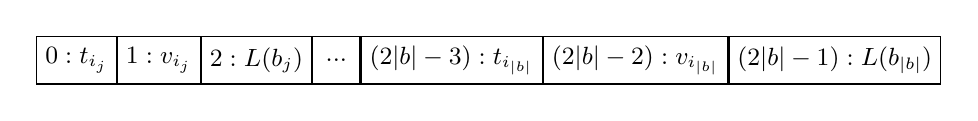
\begin{tikzpicture}
\small
\matrix[nodes={draw,minimum size=6mm}] {
  \node {$0:t_{i_j}$}; & \node {$1:v_{i_j}$}; & \node {$2:L(b_j)$}; & \node[minimum width=6mm] {...};
 &\node {$(2|b|-3):t_{i_{|b|}}$}; & \node {$(2|b|-2):v_{i_{|b|}}$}; & \node {$(2|b|-1):L(b_{|b|})$};\\
};
\end{tikzpicture}

If a waypoint has multiple labels, write them side-by-side, \textit{e.g.}
to record two labels $L_1(b_j)$ and $L_2(b_j)$ on waypoint $b_j$, write
(indices omitted for clarity):

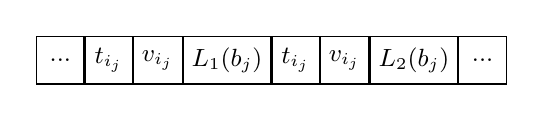
\begin{tikzpicture}
\small
\matrix[nodes={draw,minimum size=6mm}] {
  \node[minimum width=6mm] {...};
 &\node {$t_{i_j}$}; & \node {$v_{i_j}$};
 &\node {$L_1(b_j)$};
 &\node {$t_{i_j}$}; & \node {$v_{i_j}$};
 &\node {$L_2(b_j)$};
 &\node[minimum width=6mm] {...};\\
};
\end{tikzpicture}

If a waypoint has multiple labels with some indicating drop-offs, \textbf{write
the drop-offs first} before any of the pick-ups, otherwise C98 violation may
occur.\\
Array {\tt{}rid} (param. 4):&$k$-element integer array storing request identifiers
used to label \emph{new waypoints} not found in the pre-existing schedule but
found in the new remaining schedule {\tt{}sched}. The order of this array doesn't
matter.
\end{tabular}\\
\textbf{Returns:} nothing.\\
\textbf{Side Effects:} may delete and insert rows into Table W, may
update columns in Table CW, may update columns in Tables PD and CPD,
may delete and insert rows into Table CQ.\\
\textbf{Throws:} {\tt{}UserNotFoundException} if server does not exist or if
any request identifier in {\tt{}rid} (param. 4) cannot be found,
{\tt{}EdgeNotFoundException} if {\tt{}route} contains an edge that does not exist
in Table E, or {\tt{}SQLException} for other database failures.\\
\bottomrule
\end{tabular}
\nwenddocs{}\nwbegincode{135}\sublabel{NW27XAxz-y828a-1}\nwmargintag{{\nwtagstyle{}\subpageref{NW27XAxz-y828a-1}}}\moddef{Update server add to schedule~{\nwtagstyle{}\subpageref{NW27XAxz-y828a-1}}}\endmoddef\nwalsodefined{\\{NW27XAxz-y828a-2}\\{NWvbkzY-y828a-3}}\nwused{\\{NW27XAxz-4PbjF-2}\\{NWvbkzY-3YjONp-2}}
public void DBUpdateServerAddToSchedule(
    final int sid, final int[] route, final int[] sched, final int[] rid)
throws UserNotFoundException, EdgeNotFoundException, SQLException \{
  if (!this.lu_users.containsKey(sid)) \{
    throw new UserNotFoundException("User "+sid+" not found.");
  \}
  for (final int r : rid) \{
    if (!this.lu_users.containsKey(r)) \{
      throw new UserNotFoundException("User "+r+" not found.");
    \}
  \}
  Map<Integer, int[]> cache  = new HashMap<>();
  Map<Integer, int[]> cache2 = new HashMap<>();
  try (\LA{}Open \code{}conn\edoc{}~{\nwtagstyle{}\subpageref{NW27XAxz-JT1v9-1}}\RA{}) \{
    try \{
/*L1*/\LA{}..fetch \code{}sq\edoc{} and \code{}se\edoc{}~{\nwtagstyle{}\subpageref{NW27XAxz-2VNDCH-1}}\RA{}
/*L2*/\LA{}..update route~{\nwtagstyle{}\subpageref{NW27XAxz-4LV9nl-1}}\RA{}
/*L3*/\LA{}..update and add to schedule~{\nwtagstyle{}\subpageref{NW27XAxz-2VQLMF-1}}\RA{}
      conn.commit();
    \} catch (SQLException e) \{
      conn.rollback();
      throw e;
    \}
  \} catch (SQLException e) \{
    throw e;
  \}
\nosublabel{NW27XAxz-y828a-1-u4}\nwindexdefn{DBUpdateServerAddToSchedule}{DBUpdateServerAddToSchedule}{NW27XAxz-y828a-1}\eatline
\nwidentdefs{\\{{DBUpdateServerAddToSchedule}{DBUpdateServerAddToSchedule}}}\nwidentuses{\\{{lu{\char95}users}{lu:unusers}}}\nwindexuse{lu{\char95}users}{lu:unusers}{NW27XAxz-y828a-1}\nwendcode{}\nwbegindocs{136}{\small If all goes well, we add each request identifier in {\tt{}rid} into
{\tt{}\protect\nwindexuse{lu{\char95}rstatus}{lu:unrstatus}{NW27XAxz-17yXws-1}lu{\char95}rstatus} and change the value to {\tt{}true}, indicating that the request
is now \emph{assigned}.}
\nwenddocs{}\nwbegincode{137}\sublabel{NW27XAxz-y828a-2}\nwmargintag{{\nwtagstyle{}\subpageref{NW27XAxz-y828a-2}}}\moddef{Update server add to schedule~{\nwtagstyle{}\subpageref{NW27XAxz-y828a-1}}}\plusendmoddef
  for (final int r : rid) \{
    this.lu_rstatus.put(r, true);
  \}
\}
\nwidentuses{\\{{lu{\char95}rstatus}{lu:unrstatus}}}\nwindexuse{lu{\char95}rstatus}{lu:unrstatus}{NW27XAxz-y828a-2}\nwendcode{}\nwbegindocs{138}\nwdocspar
{\small After re-using some chunks from {\tt{}\protect\nwindexuse{DBUpdateServerRoute}{DBUpdateServerRoute}{NW27XAxz-4VFddh-1}DBUpdateServerRoute}(3) to update
{\tt{}route} (labels {\tt{}L1} and {\tt{}L2} above), we proceed to update {\tt{}sched}.}
\nwenddocs{}\nwbegincode{139}\sublabel{NW27XAxz-2VQLMF-1}\nwmargintag{{\nwtagstyle{}\subpageref{NW27XAxz-2VQLMF-1}}}\moddef{..update and add to schedule~{\nwtagstyle{}\subpageref{NW27XAxz-2VQLMF-1}}}\endmoddef\nwused{\\{NW27XAxz-y828a-1}}
/*a*/\LA{}....update times in pd and cpd~{\nwtagstyle{}\subpageref{NW27XAxz-1cwA5Z-1}}\RA{}
/*b*/\LA{}....populate the tp, td cache and vp, vd cache and update cq~{\nwtagstyle{}\subpageref{NW27XAxz-42MPAb-1}}\RA{}
/*c*/\LA{}....select latest order number~{\nwtagstyle{}\subpageref{NW27XAxz-1gWfDY-1}}\RA{}
/*d*/\LA{}....delete remaining schedule from cq~{\nwtagstyle{}\subpageref{NW27XAxz-4AIXfi-1}}\RA{}
/*e*/\LA{}....insert new remaining schedule into cq~{\nwtagstyle{}\subpageref{NW27XAxz-2Ir9Yx-1}}\RA{}
/*f*/\LA{}....insert into pd, cpd~{\nwtagstyle{}\subpageref{NW27XAxz-4fUZKI-1}}\RA{}
\nwendcode{}\nwbegindocs{140}\nwdocspar
{\small Just as we needed pick-up and drop-off times when updating the schedule
in {\tt{}DBupdateServerRoute}(3), we also need them here. But in addition, we
require to get the pick-up and drop-off \emph{vertices} of the new labeled
waypoints in {\tt{}sched} so that we can insert them into column \textsf{v2} in
Table PD and columns \textsf{vp} and \textsf{vd} in Table CPD. For this purpose
we introduce a second temporary map called {\tt{}cache2}.}
\nwenddocs{}\nwbegincode{141}\sublabel{NW27XAxz-42MPAb-1}\nwmargintag{{\nwtagstyle{}\subpageref{NW27XAxz-42MPAb-1}}}\moddef{....populate the tp, td cache and vp, vd cache and update cq~{\nwtagstyle{}\subpageref{NW27XAxz-42MPAb-1}}}\endmoddef\nwalsodefined{\\{NW27XAxz-42MPAb-2}\\{NW27XAxz-42MPAb-3}}\nwused{\\{NW27XAxz-2VQLMF-1}}
PreparedStatement pS140 = this.PS(conn, "S140");
for (int j = 0; j < (sched.length - 2); j += 3) \{
  final int Lj = sched[(j + 2)];
  if (Lj != sid && !cache.containsKey(Lj)) \{
    final int rq = lu_users.get(Lj)[1];
\nwidentuses{\\{{lu{\char95}users}{lu:unusers}}\\{{PS}{PS}}\\{{S140}{S140}}}\nwindexuse{lu{\char95}users}{lu:unusers}{NW27XAxz-42MPAb-1}\nwindexuse{PS}{PS}{NW27XAxz-42MPAb-1}\nwindexuse{S140}{S140}{NW27XAxz-42MPAb-1}\nwendcode{}\nwbegindocs{142}\nwdocspar
{\small If the waypoint we are working on in the {\tt{}for} loop is a new
labeled waypoint, meaning it is not found in the pre-existing remaining
schedule, then it represents a new pick-up or drop-off for some request.
We need to get both pick-up and drop-off vertices of this request so that
we can insert these values into Tables PD and CPD. We introduce a boolean
{\tt{}flagged} to detect if the waypoint is new or not.}
\nwenddocs{}\nwbegincode{143}\sublabel{NW27XAxz-42MPAb-2}\nwmargintag{{\nwtagstyle{}\subpageref{NW27XAxz-42MPAb-2}}}\moddef{....populate the tp, td cache and vp, vd cache and update cq~{\nwtagstyle{}\subpageref{NW27XAxz-42MPAb-1}}}\plusendmoddef
    boolean flagged = false;
    \LA{}......check if new job~{\nwtagstyle{}\subpageref{NW27XAxz-2Hq38w-1}}\RA{}
    if (flagged) \{
      \LA{}......get tp, vp, td, vd of new job~{\nwtagstyle{}\subpageref{NW27XAxz-pddDf-1}}\RA{}
\nwendcode{}\nwbegindocs{144}\nwdocspar
{\small If the waypoint we are working on is not a new labeled waypoint, then
we simply cache the pick-up and drop-off time as we did in
{\tt{}\protect\nosublabel{NW27XAxz-42MPAb-2-u2}\protect\nwindexuse{DBUpdateServerRoute}{DBUpdateServerRoute}{NW27XAxz-4VFddh-1}DBUpdateServerRoute}(3). At the same time we prepare and submit statement
{\tt{}\protect\nwindexuse{S140}{S140}{NW27XAxz-yno67-1}S140} to update the times in Table CQ.}
\nwenddocs{}\nwbegincode{145}\sublabel{NW27XAxz-42MPAb-3}\nwmargintag{{\nwtagstyle{}\subpageref{NW27XAxz-42MPAb-3}}}\moddef{....populate the tp, td cache and vp, vd cache and update cq~{\nwtagstyle{}\subpageref{NW27XAxz-42MPAb-1}}}\plusendmoddef
    \} else \{
      final int[] output = this.DBFetch(conn, "S86", 2, Lj);
      final int tp = output[0];
      final int td = output[1];
      this.PSAdd(pS140, tp, td, Lj);
      cache.put(Lj, new int[] \{ rq, tp, td \});
    \}
  \}
\}
this.PSSubmit(pS140);
\nwidentuses{\\{{DBFetch}{DBFetch}}\\{{PSAdd}{PSAdd}}\\{{PSSubmit}{PSSubmit}}\\{{S86}{S86}}}\nwindexuse{DBFetch}{DBFetch}{NW27XAxz-42MPAb-3}\nwindexuse{PSAdd}{PSAdd}{NW27XAxz-42MPAb-3}\nwindexuse{PSSubmit}{PSSubmit}{NW27XAxz-42MPAb-3}\nwindexuse{S86}{S86}{NW27XAxz-42MPAb-3}\nwendcode{}\nwbegindocs{146}\nwdocspar
{\small We do a linear search through {\tt{}rid} (param. 4) to determine if a
waypoint is newly labeled or not.}
\nwenddocs{}\nwbegincode{147}\sublabel{NW27XAxz-2Hq38w-1}\nwmargintag{{\nwtagstyle{}\subpageref{NW27XAxz-2Hq38w-1}}}\moddef{......check if new job~{\nwtagstyle{}\subpageref{NW27XAxz-2Hq38w-1}}}\endmoddef\nwused{\\{NW27XAxz-42MPAb-2}}
for (final int r : rid) \{
  if (Lj == r) \{
    flagged = true;
    break;
  \}
\}
\nwendcode{}\nwbegindocs{148}\nwdocspar
{\small If a waypoint is newly labeled, it can either be a new pick-up or a new
drop-off. It is a violation to have a pick-up without a drop-off or vice versa,
so we know that newly labeled waypoints come in pairs. If the label for the
waypoint we are working on doesn't appear in {\tt{}cache}, then we know the
waypoint must be a pick-up because it is the first time we've seen it.  We scan
the remainder of {\tt{}sched} to find the corresponding drop-off. Once we've found
it, we put the pick-up and drop-off times into {\tt{}cache} and the pick-up and
drop-off vertices into {\tt{}cache2}.}
\nwenddocs{}\nwbegincode{149}\sublabel{NW27XAxz-pddDf-1}\nwmargintag{{\nwtagstyle{}\subpageref{NW27XAxz-pddDf-1}}}\moddef{......get tp, vp, td, vd of new job~{\nwtagstyle{}\subpageref{NW27XAxz-pddDf-1}}}\endmoddef\nwused{\\{NW27XAxz-42MPAb-2}}
final int tp = sched[(j + 0)];
final int vp = sched[(j + 1)];
for (int k = (j + 3); k < (sched.length - 2); k += 3) \{
  if (Lj == sched[(k + 2)]) \{
    final int td = sched[(k + 0)];
    final int vd = sched[(k + 1)];
    cache. put(Lj, new int[] \{ rq, tp, td \});
    cache2.put(Lj, new int[] \{ vp, vd \});
    break;
  \}
\}
\nwendcode{}\nwbegindocs{150}\nwdocspar
{\small After re-using the chunk from {\tt{}\protect\nwindexuse{DBUpdateServerRoute}{DBUpdateServerRoute}{NW27XAxz-4VFddh-1}DBUpdateServerRoute}(3) to insert the
remaining schedule into Table CQ, we prepare and submit statements {\tt{}\protect\nwindexuse{S12}{S12}{NW27XAxz-261n0e-1}S12} and
{\tt{}\protect\nwindexuse{S13}{S13}{NW27XAxz-2Ts5w4-1}S13} to insert the new labeled waypoints into Tables PD and CPD.}
\nwenddocs{}\nwbegincode{151}\sublabel{NW27XAxz-4fUZKI-1}\nwmargintag{{\nwtagstyle{}\subpageref{NW27XAxz-4fUZKI-1}}}\moddef{....insert into pd, cpd~{\nwtagstyle{}\subpageref{NW27XAxz-4fUZKI-1}}}\endmoddef\nwused{\\{NW27XAxz-2VQLMF-1}}
PreparedStatement pS12 = this.PS(conn, "S12");
PreparedStatement pS13 = this.PS(conn, "S13");
for (final int r : rid) \{
  final int[] output2 = this.DBFetch(conn, "S51", 5, r);
  final int rq = output2[0];
  final int re = output2[1];
  final int rl = output2[2];
  final int ro = output2[3];
  final int rd = output2[4];
  final int[] qpd = cache.get(r);
  final int[]  pd = cache2.get(r);
  this.PSAdd(pS12, sid, qpd[1], pd[0], r);
  this.PSAdd(pS12, sid, qpd[2], pd[1], r);
  this.PSAdd(pS13, sid, se, route[(route.length - 2)], qpd[1], pd[0], qpd[2], pd[1],
        r, re, rl, ro, rd);
\}
this.PSSubmit(pS12, pS13);
\nwidentuses{\\{{DBFetch}{DBFetch}}\\{{PS}{PS}}\\{{PSAdd}{PSAdd}}\\{{PSSubmit}{PSSubmit}}\\{{S12}{S12}}\\{{S13}{S13}}\\{{S51}{S51}}}\nwindexuse{DBFetch}{DBFetch}{NW27XAxz-4fUZKI-1}\nwindexuse{PS}{PS}{NW27XAxz-4fUZKI-1}\nwindexuse{PSAdd}{PSAdd}{NW27XAxz-4fUZKI-1}\nwindexuse{PSSubmit}{PSSubmit}{NW27XAxz-4fUZKI-1}\nwindexuse{S12}{S12}{NW27XAxz-4fUZKI-1}\nwindexuse{S13}{S13}{NW27XAxz-4fUZKI-1}\nwindexuse{S51}{S51}{NW27XAxz-4fUZKI-1}\nwendcode{}\nwbegindocs{152}\nwdocspar

\subsection{{\tt{}\protect\nwindexuse{DBUpdateServerRemoveFromSchedule}{DBUpdateServerRemoveFromSchedule}{NW27XAxz-lMiTm-1}DBUpdateServerRemoveFromSchedule}(4)}
\begin{tabular}{p{\textwidth}}
\toprule
\rowcolor{TableTitle}
Method \textcolor{blue}{{\tt{}\protect\nwindexuse{DBUpdateServerRemoveFromSchedule}{DBUpdateServerRemoveFromSchedule}{NW27XAxz-lMiTm-1}DBUpdateServerRemoveFromSchedule}(4)} inserts a new
\emph{remaining route} for server $s$ into Table W, and a new \emph{remaining
schedule} with \emph{some pre-existing labeled waypoints removed} into Tables
PD, CPD, and CQ. If the server to be update does not exist, a
{\tt{}UserNotFoundException} is thrown.  This exception is also thrown if any
labels in the new labeled waypoints is not an existing user.  If the supplied
route contains an edge that does not exist in Table E, an
{\tt{}EdgeNotFoundException} is thrown.  A {\tt{}SQLException} is thrown for other
database failures.\\
\midrule
\textbf{Parameters:} \\
\begin{tabular}{lp{116mm}}
Integer {\tt{}sid} (param. 1):&server identifier.\\
Array {\tt{}route} (param. 2):&$2n$-element integer array storing values of
waypoint components in the server's $n$-length remaining route $w_{>t}$.
In the diagram, $|w|-i=n$.
Here $t$ is taken to be {\tt{}route[0]}. Consequently, $(t_i,v_i)$ is \emph{not} part
of the remaining route, in other words \textbf{it must pre-exist in Table W}.

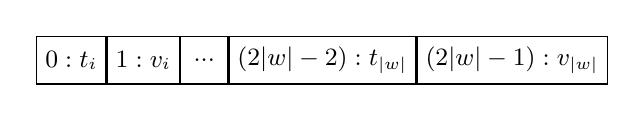
\begin{tikzpicture}
\small
\matrix[nodes={draw,minimum size=6mm}] {
  \node {$0:t_i$}; & \node {$1:v_i$}; & \node[minimum width=6mm] {...};
 &\node {$(2|w|-2):t_{|w|}$}; & \node {$(2|w|-1):v_{|w|}$}; \\
};
\end{tikzpicture}\\
Array {\tt{}sched} (param. 2):&$3m$-element integer array storing values of
waypoint components and their labels in the server's $m$-length remaining
schedule $b_{>t}$, where $m\leq n$. In the diagram, $|b|-j=m$.  Note
$(t_{i_j},v_{i_j})$ \emph{cannot equal} $(t_i,v_i)$, as $(t_i,v_i)$ is part of
the traveled route and not the remaining route (we cannot change the past).
Therefore $t_{i_j}$ \textbf{must be greater than} $t_i$. Due to rule R3,
$(t_{i_{|b|}},v_{i_{|b|}})$ \textbf{must equal} $(t_{|w|},v_{|w|})$.

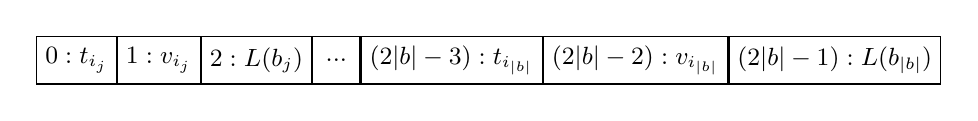
\begin{tikzpicture}
\small
\matrix[nodes={draw,minimum size=6mm}] {
  \node {$0:t_{i_j}$}; & \node {$1:v_{i_j}$}; & \node {$2:L(b_j)$}; & \node[minimum width=6mm] {...};
 &\node {$(2|b|-3):t_{i_{|b|}}$}; & \node {$(2|b|-2):v_{i_{|b|}}$}; & \node {$(2|b|-1):L(b_{|b|})$};\\
};
\end{tikzpicture}

If a waypoint has multiple labels, write them side-by-side, \textit{e.g.}
to record two labels $L_1(b_j)$ and $L_2(b_j)$ on waypoint $b_j$, write
(indices omitted for clarity):

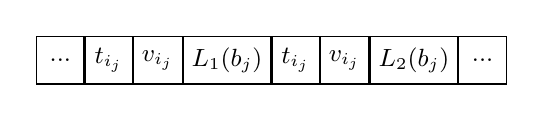
\begin{tikzpicture}
\small
\matrix[nodes={draw,minimum size=6mm}] {
  \node[minimum width=6mm] {...};
 &\node {$t_{i_j}$}; & \node {$v_{i_j}$};
 &\node {$L_1(b_j)$};
 &\node {$t_{i_j}$}; & \node {$v_{i_j}$};
 &\node {$L_2(b_j)$};
 &\node[minimum width=6mm] {...};\\
};
\end{tikzpicture}

If a waypoint has multiple labels with some indicating drop-offs, \textbf{write
the drop-offs first} before any of the pick-ups, otherwise C98 violation may
occur.\\ Array {\tt{}rid} (param. 4):&$k$-element integer array storing request
identifiers found in the pre-existing schedule \emph{but not found in the new
remaining schedule} {\tt{}sched}. The order of this array doesn't matter.
\end{tabular}\\
\textbf{Returns:} nothing.\\
\textbf{Side Effects:} may delete and insert rows into Table W, may
update columns in Table CW, may update columns in Tables PD and CPD,
may delete and insert rows into Table CQ.\\
\textbf{Throws:} {\tt{}UserNotFoundException} if server does not exist or if
any request identifier in {\tt{}rid} (param. 4) cannot be found,
{\tt{}EdgeNotFoundException} if {\tt{}route} contains an edge that does not exist
in Table E, or {\tt{}SQLException} for other database failures.\\
\bottomrule
\end{tabular}
\nwenddocs{}\nwbegincode{153}\sublabel{NW27XAxz-lMiTm-1}\nwmargintag{{\nwtagstyle{}\subpageref{NW27XAxz-lMiTm-1}}}\moddef{Update server remove from schedule~{\nwtagstyle{}\subpageref{NW27XAxz-lMiTm-1}}}\endmoddef\nwalsodefined{\\{NW27XAxz-lMiTm-2}\\{NWvbkzY-lMiTm-3}}\nwused{\\{NW27XAxz-4PbjF-2}\\{NWvbkzY-3YjONp-2}}
public void DBUpdateServerRemoveFromSchedule(
    final int sid, final int[] route, final int[] sched, final int[] rid)
throws UserNotFoundException, EdgeNotFoundException, SQLException \{
  if (!this.lu_users.containsKey(sid)) \{
    throw new UserNotFoundException("User "+sid+" not found.");
  \}
  for (final int r : rid) \{
    if (!this.lu_users.containsKey(r)) \{
      throw new UserNotFoundException("User "+r+" not found.");
    \}
  \}
  Map<Integer, int[]> cache = new HashMap<>();
  try (\LA{}Open \code{}conn\edoc{}~{\nwtagstyle{}\subpageref{NW27XAxz-JT1v9-1}}\RA{}) \{
    try \{
/*L1*/\LA{}..fetch \code{}sq\edoc{} and \code{}se\edoc{}~{\nwtagstyle{}\subpageref{NW27XAxz-2VNDCH-1}}\RA{}
/*L2*/\LA{}..update route~{\nwtagstyle{}\subpageref{NW27XAxz-4LV9nl-1}}\RA{}
/*L3*/\LA{}..update schedule~{\nwtagstyle{}\subpageref{NW27XAxz-2NqWTJ-1}}\RA{}
/*L4*/\LA{}..remove jobs from pd, cpd~{\nwtagstyle{}\subpageref{NW27XAxz-2PX0wC-1}}\RA{}
      conn.commit();
    \} catch (SQLException e) \{
      conn.rollback();
      throw e;
    \}
  \} catch (SQLException e) \{
    throw e;
  \}
\nosublabel{NW27XAxz-lMiTm-1-u5}\nwindexdefn{DBUpdateServerRemoveFromSchedule}{DBUpdateServerRemoveFromSchedule}{NW27XAxz-lMiTm-1}\eatline
\nwidentdefs{\\{{DBUpdateServerRemoveFromSchedule}{DBUpdateServerRemoveFromSchedule}}}\nwidentuses{\\{{lu{\char95}users}{lu:unusers}}}\nwindexuse{lu{\char95}users}{lu:unusers}{NW27XAxz-lMiTm-1}\nwendcode{}\nwbegindocs{154}{\small If all goes well, we put each request indentifier in {\tt{}rid} into
{\tt{}\protect\nwindexuse{lu{\char95}rstatus}{lu:unrstatus}{NW27XAxz-17yXws-1}lu{\char95}rstatus} and change the value to {\tt{}false}, indicating that the request
is now \emph{unassigned}.}
\nwenddocs{}\nwbegincode{155}\sublabel{NW27XAxz-lMiTm-2}\nwmargintag{{\nwtagstyle{}\subpageref{NW27XAxz-lMiTm-2}}}\moddef{Update server remove from schedule~{\nwtagstyle{}\subpageref{NW27XAxz-lMiTm-1}}}\plusendmoddef
  for (final int r : rid) \{
    this.lu_rstatus.put(r, false);
  \}
\}
\nwidentuses{\\{{lu{\char95}rstatus}{lu:unrstatus}}}\nwindexuse{lu{\char95}rstatus}{lu:unrstatus}{NW27XAxz-lMiTm-2}\nwendcode{}\nwbegindocs{156}\nwdocspar
{\small We re-use chunks from {\tt{}\protect\nwindexuse{DBUpdateServerRoute}{DBUpdateServerRoute}{NW27XAxz-4VFddh-1}DBUpdateServerRoute}(3) to update the route
and the schedule. Then we prepare and submit statements {\tt{}\protect\nwindexuse{S42}{S42}{NW27XAxz-25mK0a-1}S42} and {\tt{}\protect\nwindexuse{S43}{S43}{NW27XAxz-2Tccw0-1}S43} to
delete labeled waypoints from Tables PD and CPD.}
\nwenddocs{}\nwbegincode{157}\sublabel{NW27XAxz-2PX0wC-1}\nwmargintag{{\nwtagstyle{}\subpageref{NW27XAxz-2PX0wC-1}}}\moddef{..remove jobs from pd, cpd~{\nwtagstyle{}\subpageref{NW27XAxz-2PX0wC-1}}}\endmoddef\nwused{\\{NW27XAxz-lMiTm-1}}
PreparedStatement pS42 = this.PS(conn, "S42");
PreparedStatement pS43 = this.PS(conn, "S43");
for (final int r : rid) \{
  this.PSAdd(pS42, r);
  this.PSAdd(pS43, r);
\}
this.PSSubmit(pS42, pS43);
\nwidentuses{\\{{PS}{PS}}\\{{PSAdd}{PSAdd}}\\{{PSSubmit}{PSSubmit}}\\{{S42}{S42}}\\{{S43}{S43}}}\nwindexuse{PS}{PS}{NW27XAxz-2PX0wC-1}\nwindexuse{PSAdd}{PSAdd}{NW27XAxz-2PX0wC-1}\nwindexuse{PSSubmit}{PSSubmit}{NW27XAxz-2PX0wC-1}\nwindexuse{S42}{S42}{NW27XAxz-2PX0wC-1}\nwindexuse{S43}{S43}{NW27XAxz-2PX0wC-1}\nwendcode{}\nwbegindocs{158}\nwdocspar

\subsection{Read Methods}
\label{sec:read-methods}

\subsection{{\tt{}\protect\nwindexuse{DBQuery}{DBQuery}{NW27XAxz-2FtqIZ-2}DBQuery}(2)}
\begin{tabular}{p{\textwidth}}
\toprule
\rowcolor{TableTitle}
Method \textcolor{blue}{{\tt{}\protect\nwindexuse{DBQuery}{DBQuery}{NW27XAxz-2FtqIZ-2}DBQuery}}(2) executes an arbitrary {\tt{}SELECT}
query against the Jargo database instance.
A {\tt{}SQLException} is thrown in case of database failure.\\
\midrule
\textbf{Parameters:} \\
\begin{tabular}{lp{116mm}}
String {\tt{}sql} (param. 1):&{\tt{}SELECT} statement to execute.\\
Integer {\tt{}ncols} (param. 2):&number of columns $n$ in the selection.\\
\end{tabular}
\textbf{Returns:} results of the query flattened into an integer array,
or {\tt{}null} if no results.

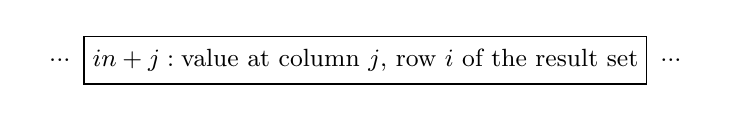
\begin{tikzpicture}
\small
\matrix[nodes={minimum size=6mm}] {
  \node {...};
 &\node[draw] {$in+j:\textrm{value at column $j$, row $i$ of the result set}$};
 &\node {...};\\
};
\end{tikzpicture}

where $i$, $j$ start from 0.\\
\textbf{Side Effects:} none.\\
\textbf{Throws:} {\tt{}SQLException} if database failure is encountered.\\
\bottomrule
\end{tabular}
\nwenddocs{}\nwbegincode{159}\sublabel{NW27XAxz-2FtqIZ-1}\nwmargintag{{\nwtagstyle{}\subpageref{NW27XAxz-2FtqIZ-1}}}\moddef{Query custom statement~{\nwtagstyle{}\subpageref{NW27XAxz-2FtqIZ-1}}}\endmoddef\nwalsodefined{\\{NW27XAxz-2FtqIZ-2}\\{NW2ZDXo8-2FtqIZ-3}}\nwused{\\{NW27XAxz-4PbjF-1}\\{NW2ZDXo8-bF3Hn-2}}
public int[] DBQuery(final String sql, final int ncols) throws SQLException \{
  int[] output = new int[] \{ \};
  try (\LA{}Open \code{}conn\edoc{}~{\nwtagstyle{}\subpageref{NW27XAxz-JT1v9-1}}\RA{}) \{
    Statement stmt = conn.createStatement(
      ResultSet.TYPE_SCROLL_INSENSITIVE, ResultSet.CONCUR_READ_ONLY);
    ResultSet res = stmt.executeQuery(sql);
\nwidentuses{\\{{DBQuery}{DBQuery}}}\nwindexuse{DBQuery}{DBQuery}{NW27XAxz-2FtqIZ-1}\nwendcode{}\nwbegindocs{160}\nwdocspar
{\small The JDBC method {\tt{}ResultSet.last}(0) returns {\tt{}false} if there are no
results.  We use the return value to determine whether or not to continue
flattening results.}
\nwenddocs{}\nwbegincode{161}\sublabel{NW27XAxz-2FtqIZ-2}\nwmargintag{{\nwtagstyle{}\subpageref{NW27XAxz-2FtqIZ-2}}}\moddef{Query custom statement~{\nwtagstyle{}\subpageref{NW27XAxz-2FtqIZ-1}}}\plusendmoddef
    if (res.last()) \{
      \LA{}..flatten results~{\nwtagstyle{}\subpageref{NW27XAxz-2Xu6MS-1}}\RA{}
    \}
    conn.close();
  \} catch (SQLException e) \{
    throw e;
  \}
  return output;
\}
\nosublabel{NW27XAxz-2FtqIZ-2-u1}\nwindexdefn{DBQuery}{DBQuery}{NW27XAxz-2FtqIZ-2}\eatline
\nwidentdefs{\\{{DBQuery}{DBQuery}}}\nwendcode{}\nwbegindocs{162}{\small In the flattening procedure, we simply loop through the result rows and
columns, adding values into their respective positions in the returned
{\tt{}output} array.}
\nwenddocs{}\nwbegincode{163}\sublabel{NW27XAxz-2Xu6MS-1}\nwmargintag{{\nwtagstyle{}\subpageref{NW27XAxz-2Xu6MS-1}}}\moddef{..flatten results~{\nwtagstyle{}\subpageref{NW27XAxz-2Xu6MS-1}}}\endmoddef\nwused{\\{NW27XAxz-2FtqIZ-2}\\{NW27XAxz-17Zt8W-1}}
output = new int[(ncols*res.getRow())];
res.first();
do \{
  for (int j = 1; j <= ncols; j++) \{
    output[((res.getRow() - 1)*ncols + (j - 1))] = res.getInt(j);
  \}
\} while (res.next());
\nwendcode{}\nwbegindocs{164}\nwdocspar

\subsection{{\tt{}\protect\nwindexuse{DBQueryCountVertices}{DBQueryCountVertices}{NW27XAxz-2YwxVt-1}DBQueryCountVertices}(0)}
\begin{tabular}{p{\textwidth}}
\toprule
\rowcolor{TableTitle}
Method \textcolor{blue}{{\tt{}\protect\nwindexuse{DBQueryCountVertices}{DBQueryCountVertices}{NW27XAxz-2YwxVt-1}DBQueryCountVertices}}(0) returns the total number
of vertices in Table V.
A {\tt{}SQLException} is thrown in case of database failure.\\
\midrule
\textbf{Parameters:} none.\\
\textbf{Returns:} results of the query flattened into an integer array, or
{\tt{}null} if no results.

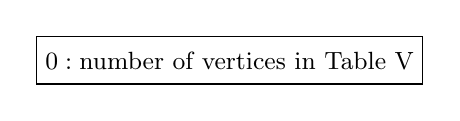
\begin{tikzpicture}
\small
\matrix[nodes={draw,minimum size=6mm}] {
  \node {$0:\textrm{number of vertices in Table V}$};\\
};
\end{tikzpicture}\\
\textbf{Side Effects:} none.\\
\textbf{Throws:} {\tt{}SQLException} if database failure is encountered.\\
\bottomrule
\end{tabular}
\nwenddocs{}\nwbegincode{165}\sublabel{NW27XAxz-2YwxVt-1}\nwmargintag{{\nwtagstyle{}\subpageref{NW27XAxz-2YwxVt-1}}}\moddef{Query count of vertices~{\nwtagstyle{}\subpageref{NW27XAxz-2YwxVt-1}}}\endmoddef\nwused{\\{NW27XAxz-4PbjF-1}}
public int[] DBQueryCountVertices() throws SQLException \{
  try (\LA{}Open \code{}conn\edoc{}~{\nwtagstyle{}\subpageref{NW27XAxz-JT1v9-1}}\RA{}) \{
    return this.DBFetch(conn, "S62", 1);
  \} catch (SQLException e) \{
    throw e;
  \}
\}
\nwindexdefn{DBQueryCountVertices}{DBQueryCountVertices}{NW27XAxz-2YwxVt-1}\eatline
\nwidentdefs{\\{{DBQueryCountVertices}{DBQueryCountVertices}}}\nwidentuses{\\{{DBFetch}{DBFetch}}\\{{S62}{S62}}}\nwindexuse{DBFetch}{DBFetch}{NW27XAxz-2YwxVt-1}\nwindexuse{S62}{S62}{NW27XAxz-2YwxVt-1}\nwendcode{}\nwbegindocs{166}\nwdocspar
\subsection{{\tt{}\protect\nwindexuse{DBQueryCountEdges}{DBQueryCountEdges}{NW27XAxz-1SFiNd-1}DBQueryCountEdges}(0)}
\begin{tabular}{p{\textwidth}}
\toprule
\rowcolor{TableTitle}
Method \textcolor{blue}{{\tt{}\protect\nwindexuse{DBQueryCountEdges}{DBQueryCountEdges}{NW27XAxz-1SFiNd-1}DBQueryCountEdges}}(0) returns the total number
of vertices in Table V.
A {\tt{}SQLException} is thrown in case of database failure.\\
\midrule
\textbf{Parameters:} none.\\
\textbf{Returns:} results of the query flattened into an integer array, or
{\tt{}null} if no results.

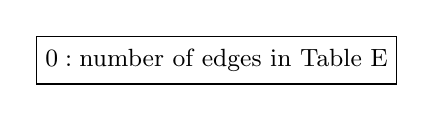
\begin{tikzpicture}
\small
\matrix[nodes={draw,minimum size=6mm}] {
  \node {$0:\textrm{number of edges in Table E}$};\\
};
\end{tikzpicture}\\
\textbf{Side Effects:} none.\\
\textbf{Throws:} {\tt{}SQLException} if database failure is encountered.\\
\bottomrule
\end{tabular}
\nwenddocs{}\nwbegincode{167}\sublabel{NW27XAxz-1SFiNd-1}\nwmargintag{{\nwtagstyle{}\subpageref{NW27XAxz-1SFiNd-1}}}\moddef{Query count of edges~{\nwtagstyle{}\subpageref{NW27XAxz-1SFiNd-1}}}\endmoddef\nwused{\\{NW27XAxz-4PbjF-1}}
public int[] DBQueryCountEdges() throws SQLException \{
  try (\LA{}Open \code{}conn\edoc{}~{\nwtagstyle{}\subpageref{NW27XAxz-JT1v9-1}}\RA{}) \{
    return this.DBFetch(conn, "S63", 1);
  \} catch (SQLException e) \{
    throw e;
  \}
\}
\nwindexdefn{DBQueryCountEdges}{DBQueryCountEdges}{NW27XAxz-1SFiNd-1}\eatline
\nwidentdefs{\\{{DBQueryCountEdges}{DBQueryCountEdges}}}\nwidentuses{\\{{DBFetch}{DBFetch}}\\{{S63}{S63}}}\nwindexuse{DBFetch}{DBFetch}{NW27XAxz-1SFiNd-1}\nwindexuse{S63}{S63}{NW27XAxz-1SFiNd-1}\nwendcode{}\nwbegindocs{168}\nwdocspar
\subsection{{\tt{}\protect\nwindexuse{DBQueryVertex}{DBQueryVertex}{NW27XAxz-4IfXsG-1}DBQueryVertex}(1)}
\begin{tabular}{p{\textwidth}}
\toprule
\rowcolor{TableTitle}
Method \textcolor{blue}{{\tt{}\protect\nwindexuse{DBQueryVertex}{DBQueryVertex}{NW27XAxz-4IfXsG-1}DBQueryVertex}}(1) returns the longitude and
latitude coordinates of the given vertex. If the vertex does not exist,
a {\tt{}VertexNotFoundException} is thrown.\\
\midrule
\textbf{Parameters:} \\
\begin{tabular}{lp{116mm}}
Integer {\tt{}v} (param. 1):&vertex identifier.
\end{tabular}
\textbf{Returns:} results of the query flattened into an integer array, or
{\tt{}null} if no results.

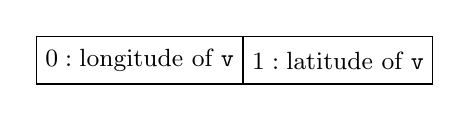
\begin{tikzpicture}
\small
\matrix[nodes={draw,minimum size=6mm}] {
  \node {$0:\textrm{longitude of }\texttt{v}$};
 &\node {$1:\textrm{latitude of }\texttt{v}$};\\
};
\end{tikzpicture}\\
\textbf{Side Effects:} none.\\
\textbf{Throws:} {\tt{}VertexNotFoundException} if vertex does not exist\\
\bottomrule
\end{tabular}
\nwenddocs{}\nwbegincode{169}\sublabel{NW27XAxz-4IfXsG-1}\nwmargintag{{\nwtagstyle{}\subpageref{NW27XAxz-4IfXsG-1}}}\moddef{Query vertex~{\nwtagstyle{}\subpageref{NW27XAxz-4IfXsG-1}}}\endmoddef\nwalsodefined{\\{NW2ZDXo8-4IfXsG-2}\\{NWvbkzY-4IfXsG-3}}\nwused{\\{NW27XAxz-4PbjF-1}\\{NW2ZDXo8-bF3Hn-2}\\{NWvbkzY-3YjONp-3}}
public int[] DBQueryVertex(final int v) throws VertexNotFoundException \{
  if (!this.lu_vertices.containsKey(v)) \{
    throw new VertexNotFoundException("Vertex "+v+" not found.");
  \}
  return this.lu_vertices.get(v).clone();
\}
\nwindexdefn{DBQueryVertex}{DBQueryVertex}{NW27XAxz-4IfXsG-1}\eatline
\nwidentdefs{\\{{DBQueryVertex}{DBQueryVertex}}}\nwidentuses{\\{{lu{\char95}vertices}{lu:unvertices}}}\nwindexuse{lu{\char95}vertices}{lu:unvertices}{NW27XAxz-4IfXsG-1}\nwendcode{}\nwbegindocs{170}\nwdocspar
\subsection{{\tt{}\protect\nwindexuse{DBQueryAllVertices}{DBQueryAllVertices}{NW27XAxz-1r5OnM-1}DBQueryAllVertices}(0)}
\begin{tabular}{p{\textwidth}}
\toprule
\rowcolor{TableTitle}
Method \textcolor{blue}{{\tt{}\protect\nwindexuse{DBQueryAllVertices}{DBQueryAllVertices}{NW27XAxz-1r5OnM-1}DBQueryAllVertices}}(0) returns all rows in Table V.
A {\tt{}SQLException} is thrown in case of database failure.\\
\midrule
\textbf{Parameters:} none.\\
\textbf{Returns:} results of the query flattened into an integer array, or
{\tt{}null} if no results.

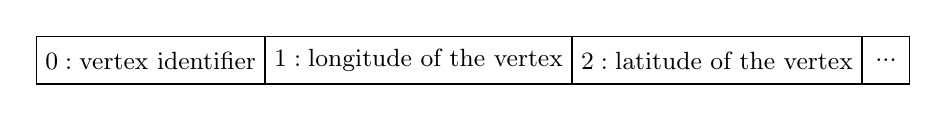
\begin{tikzpicture}
\small
\matrix[nodes={draw,minimum size=6mm}] {
  \node {$0:\textrm{vertex identifier}$};
 &\node {$1:\textrm{longitude of the vertex}$};
 &\node {$2:\textrm{latitude of the vertex}$};
 &\node {...};\\
};
\end{tikzpicture}\\
\textbf{Side Effects:} none.\\
\textbf{Throws:} {\tt{}SQLException} if database failure is encountered.\\
\bottomrule
\end{tabular}
\nwenddocs{}\nwbegincode{171}\sublabel{NW27XAxz-1r5OnM-1}\nwmargintag{{\nwtagstyle{}\subpageref{NW27XAxz-1r5OnM-1}}}\moddef{Query all vertices~{\nwtagstyle{}\subpageref{NW27XAxz-1r5OnM-1}}}\endmoddef\nwalsodefined{\\{NW2ZDXo8-1r5OnM-2}}\nwused{\\{NW27XAxz-4PbjF-1}\\{NW2ZDXo8-bF3Hn-2}}
public int[] DBQueryAllVertices() throws SQLException \{
  try (\LA{}Open \code{}conn\edoc{}~{\nwtagstyle{}\subpageref{NW27XAxz-JT1v9-1}}\RA{}) \{
    return this.DBFetch(conn, "S136", 3);
  \} catch (SQLException e) \{
    throw e;
  \}
\}
\nwindexdefn{DBQueryAllVertices}{DBQueryAllVertices}{NW27XAxz-1r5OnM-1}\eatline
\nwidentdefs{\\{{DBQueryAllVertices}{DBQueryAllVertices}}}\nwidentuses{\\{{DBFetch}{DBFetch}}\\{{S136}{S136}}}\nwindexuse{DBFetch}{DBFetch}{NW27XAxz-1r5OnM-1}\nwindexuse{S136}{S136}{NW27XAxz-1r5OnM-1}\nwendcode{}\nwbegindocs{172}\nwdocspar
\subsection{{\tt{}\protect\nwindexuse{DBQueryEdge}{DBQueryEdge}{NW27XAxz-1E2aru-1}DBQueryEdge}(2)}
\begin{tabular}{p{\textwidth}}
\toprule
\rowcolor{TableTitle}
Method \textcolor{blue}{{\tt{}\protect\nwindexuse{DBQueryEdge}{DBQueryEdge}{NW27XAxz-1E2aru-1}DBQueryEdge}}(2) returns the distance and
maximum free-flow speed along the given edge.
An {\tt{}EdgeNotFoundException} is thrown if the edge does not exist.\\
\midrule
\textbf{Parameters:} \\
\begin{tabular}{lp{116mm}}
Integer {\tt{}v1} (param. 1):&source vertex identifier $v_1$\\
Integer {\tt{}v2} (param. 2):&target vertex identifier $v_2$
\end{tabular}\\
\textbf{Returns:} results of the query flattened into an integer array, or
{\tt{}null} if no results.

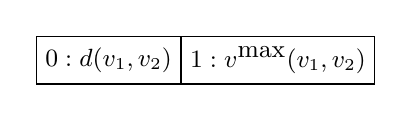
\begin{tikzpicture}
\small
\matrix[nodes={draw,minimum size=6mm}] {
  \node {$0:d(v_1,v_2)$}; & \node {$1:v^\textrm{max}(v_1,v_2)$}; \\
};
\end{tikzpicture}\\
\textbf{Side Effects:} none.\\
\textbf{Throws:} {\tt{}EdgeNotFoundException} if edge does not exit.\\
\bottomrule
\end{tabular}
\nwenddocs{}\nwbegincode{173}\sublabel{NW27XAxz-1E2aru-1}\nwmargintag{{\nwtagstyle{}\subpageref{NW27XAxz-1E2aru-1}}}\moddef{Query edge~{\nwtagstyle{}\subpageref{NW27XAxz-1E2aru-1}}}\endmoddef\nwalsodefined{\\{NW2ZDXo8-1E2aru-2}\\{NWvbkzY-1E2aru-3}}\nwused{\\{NW27XAxz-4PbjF-1}\\{NW2ZDXo8-bF3Hn-2}\\{NWvbkzY-3YjONp-3}}
public int[] DBQueryEdge(final int v1, final int v2) throws EdgeNotFoundException \{
  if (!(this.lu_edges.containsKey(v1) && this.lu_edges.get(v1).containsKey(v2))) \{
    throw new EdgeNotFoundException("Edge ("+v1+", "+v2+") not found.");
  \}
  return this.lu_edges.get(v1).get(v2).clone();
\}
\nwindexdefn{DBQueryEdge}{DBQueryEdge}{NW27XAxz-1E2aru-1}\eatline
\nwidentdefs{\\{{DBQueryEdge}{DBQueryEdge}}}\nwidentuses{\\{{lu{\char95}edges}{lu:unedges}}}\nwindexuse{lu{\char95}edges}{lu:unedges}{NW27XAxz-1E2aru-1}\nwendcode{}\nwbegindocs{174}\nwdocspar
\subsection{{\tt{}\protect\nwindexuse{DBQueryAllEdges}{DBQueryAllEdges}{NW27XAxz-4ILREc-1}DBQueryAllEdges}(0)}
\begin{tabular}{p{\textwidth}}
\toprule
\rowcolor{TableTitle}
Method \textcolor{blue}{{\tt{}\protect\nwindexuse{DBQueryAllEdges}{DBQueryAllEdges}{NW27XAxz-4ILREc-1}DBQueryAllEdges}}(0) returns all rows in Table E.
A {\tt{}SQLException} is thrown in case of database failure.\\
\midrule
\textbf{Parameters:} none.\\
\textbf{Returns:} results of the query flattened into an integer array, or
{\tt{}null} if no results.

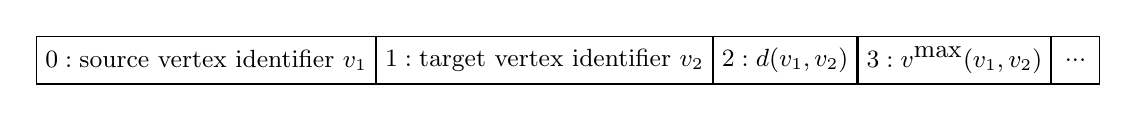
\begin{tikzpicture}
\small
\matrix[nodes={draw,minimum size=6mm}] {
  \node {$0:\textrm{source vertex identifier $v_1$}$};
 &\node {$1:\textrm{target vertex identifier $v_2$}$};
 &\node {$2:d(v_1,v_2)$};
 &\node {$3:v^\textrm{max}(v_1,v_2)$};
 &\node {...};\\
};
\end{tikzpicture}\\
\textbf{Side Effects:} none.\\
\textbf{Throws:} {\tt{}SQLException} if database failure is encountered.\\
\bottomrule
\end{tabular}
\nwenddocs{}\nwbegincode{175}\sublabel{NW27XAxz-4ILREc-1}\nwmargintag{{\nwtagstyle{}\subpageref{NW27XAxz-4ILREc-1}}}\moddef{Query all edges~{\nwtagstyle{}\subpageref{NW27XAxz-4ILREc-1}}}\endmoddef\nwalsodefined{\\{NW2ZDXo8-4ILREc-2}}\nwused{\\{NW27XAxz-4PbjF-1}\\{NW2ZDXo8-bF3Hn-2}}
public int[] DBQueryAllEdges() throws SQLException \{
  try (\LA{}Open \code{}conn\edoc{}~{\nwtagstyle{}\subpageref{NW27XAxz-JT1v9-1}}\RA{}) \{
    return this.DBFetch(conn, "S137", 4);
  \} catch (SQLException e) \{
    throw e;
  \}
\}
\nwindexdefn{DBQueryAllEdges}{DBQueryAllEdges}{NW27XAxz-4ILREc-1}\eatline
\nwidentdefs{\\{{DBQueryAllEdges}{DBQueryAllEdges}}}\nwidentuses{\\{{DBFetch}{DBFetch}}\\{{S137}{S137}}}\nwindexuse{DBFetch}{DBFetch}{NW27XAxz-4ILREc-1}\nwindexuse{S137}{S137}{NW27XAxz-4ILREc-1}\nwendcode{}\nwbegindocs{176}\nwdocspar
\subsection{{\tt{}\protect\nwindexuse{DBQueryStatisticsEdges}{DBQueryStatisticsEdges}{NW27XAxz-F2Kkr-1}DBQueryStatisticsEdges}(0)}
\begin{tabular}{p{\textwidth}}
\toprule
\rowcolor{TableTitle}
Method \textcolor{blue}{{\tt{}\protect\nwindexuse{DBQueryStatisticsEdges}{DBQueryStatisticsEdges}{NW27XAxz-F2Kkr-1}DBQueryStatisticsEdges}}(0) returns some edge statistics.
A {\tt{}SQLException} is thrown in case of database failure.\\
\midrule
\textbf{Parameters:} none.\\
\textbf{Returns:} results of the query flattened into an integer array, or
{\tt{}null} if no results.

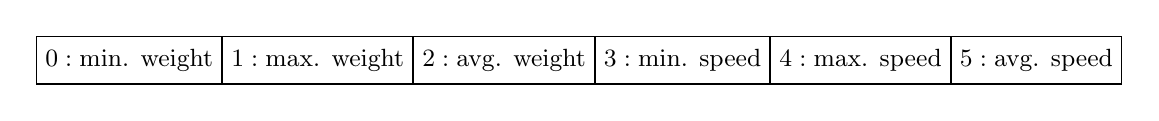
\begin{tikzpicture}
\small
\matrix[nodes={draw,minimum size=6mm}] {
  \node {$0:\textrm{min. weight}$};
 &\node {$1:\textrm{max. weight}$};
 &\node {$2:\textrm{avg. weight}$};
 &\node {$3:\textrm{min. speed}$};
 &\node {$4:\textrm{max. speed}$};
 &\node {$5:\textrm{avg. speed}$};\\
};
\end{tikzpicture}\\
\textbf{Side Effects:} none.\\
\textbf{Throws:} {\tt{}SQLException} if database failure is encountered.\\
\bottomrule
\end{tabular}
\nwenddocs{}\nwbegincode{177}\sublabel{NW27XAxz-F2Kkr-1}\nwmargintag{{\nwtagstyle{}\subpageref{NW27XAxz-F2Kkr-1}}}\moddef{Query edge statistics~{\nwtagstyle{}\subpageref{NW27XAxz-F2Kkr-1}}}\endmoddef\nwused{\\{NW27XAxz-4PbjF-1}}
public int[] DBQueryStatisticsEdges() throws SQLException \{
  try (\LA{}Open \code{}conn\edoc{}~{\nwtagstyle{}\subpageref{NW27XAxz-JT1v9-1}}\RA{}) \{
    return this.DBFetch(conn, "S65", 6);
  \} catch (SQLException e) \{
    throw e;
  \}
\}
\nwindexdefn{DBQueryStatisticsEdges}{DBQueryStatisticsEdges}{NW27XAxz-F2Kkr-1}\eatline
\nwidentdefs{\\{{DBQueryStatisticsEdges}{DBQueryStatisticsEdges}}}\nwidentuses{\\{{DBFetch}{DBFetch}}\\{{S65}{S65}}}\nwindexuse{DBFetch}{DBFetch}{NW27XAxz-F2Kkr-1}\nwindexuse{S65}{S65}{NW27XAxz-F2Kkr-1}\nwendcode{}\nwbegindocs{178}\nwdocspar
\subsection{{\tt{}\protect\nwindexuse{DBQueryMBR}{DBQueryMBR}{NW27XAxz-234rWd-1}DBQueryMBR}(0)}
\begin{tabular}{p{\textwidth}}
\toprule
\rowcolor{TableTitle}
Method \textcolor{blue}{{\tt{}\protect\nwindexuse{DBQueryMBR}{DBQueryMBR}{NW27XAxz-234rWd-1}DBQueryMBR}}(0) returns the minimum-bounding
rectangle of the road network.
A {\tt{}SQLException} is thrown in case of database failure.\\
\midrule
\textbf{Parameters:} none.\\
\textbf{Returns:} results of the query flattened into an integer array, or
{\tt{}null} if no results.

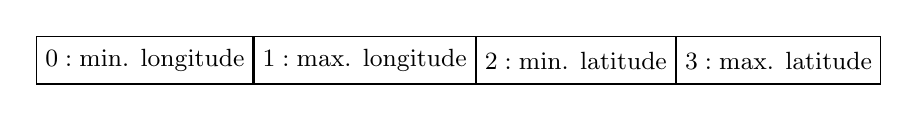
\begin{tikzpicture}
\small
\matrix[nodes={draw,minimum size=6mm}] {
  \node {$0:\textrm{min. longitude}$};
 &\node {$1:\textrm{max. longitude}$};
 &\node {$2:\textrm{min. latitude}$};
 &\node {$3:\textrm{max. latitude}$};\\
};
\end{tikzpicture}\\
\textbf{Side Effects:} none.\\
\textbf{Throws:} {\tt{}SQLException} if database failure is encountered.\\
\bottomrule
\end{tabular}
\nwenddocs{}\nwbegincode{179}\sublabel{NW27XAxz-234rWd-1}\nwmargintag{{\nwtagstyle{}\subpageref{NW27XAxz-234rWd-1}}}\moddef{Query MBR~{\nwtagstyle{}\subpageref{NW27XAxz-234rWd-1}}}\endmoddef\nwused{\\{NW27XAxz-4PbjF-1}}
public int[] DBQueryMBR() throws SQLException \{
  try (\LA{}Open \code{}conn\edoc{}~{\nwtagstyle{}\subpageref{NW27XAxz-JT1v9-1}}\RA{}) \{
    return this.DBFetch(conn, "S64", 4);
  \} catch (SQLException e) \{
    throw e;
  \}
\}
\nwindexdefn{DBQueryMBR}{DBQueryMBR}{NW27XAxz-234rWd-1}\eatline
\nwidentdefs{\\{{DBQueryMBR}{DBQueryMBR}}}\nwidentuses{\\{{DBFetch}{DBFetch}}\\{{S64}{S64}}}\nwindexuse{DBFetch}{DBFetch}{NW27XAxz-234rWd-1}\nwindexuse{S64}{S64}{NW27XAxz-234rWd-1}\nwendcode{}\nwbegindocs{180}\nwdocspar
\subsection{{\tt{}\protect\nwindexuse{DBQueryCountServers}{DBQueryCountServers}{NW27XAxz-2FrFih-1}DBQueryCountServers}(0)}
\begin{tabular}{p{\textwidth}}
\toprule
\rowcolor{TableTitle}
Method \textcolor{blue}{{\tt{}DBQueryCountSevers}}(0) returns the total number
of servers in Table S.
A {\tt{}SQLException} is thrown in case of database failure.\\
\midrule
\textbf{Parameters:} none.\\
\textbf{Returns:} results of the query flattened into an integer array, or
{\tt{}null} if no results.

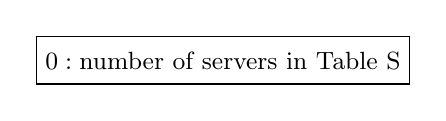
\begin{tikzpicture}
\small
\matrix[nodes={draw,minimum size=6mm}] {
  \node {$0:\textrm{number of servers in Table S}$};\\
};
\end{tikzpicture}\\
\textbf{Side Effects:} none.\\
\textbf{Throws:} {\tt{}SQLException} if database failure is encountered.\\
\bottomrule
\end{tabular}
\nwenddocs{}\nwbegincode{181}\sublabel{NW27XAxz-2FrFih-1}\nwmargintag{{\nwtagstyle{}\subpageref{NW27XAxz-2FrFih-1}}}\moddef{Query count of servers~{\nwtagstyle{}\subpageref{NW27XAxz-2FrFih-1}}}\endmoddef\nwused{\\{NW27XAxz-4PbjF-1}}
public int[] DBQueryCountServers() throws SQLException \{
  try (\LA{}Open \code{}conn\edoc{}~{\nwtagstyle{}\subpageref{NW27XAxz-JT1v9-1}}\RA{}) \{
    return this.DBFetch(conn, "S66", 1);
  \} catch (SQLException e) \{
    throw e;
  \}
\}
\nwindexdefn{DBQueryCountServers}{DBQueryCountServers}{NW27XAxz-2FrFih-1}\eatline
\nwidentdefs{\\{{DBQueryCountServers}{DBQueryCountServers}}}\nwidentuses{\\{{DBFetch}{DBFetch}}\\{{S66}{S66}}}\nwindexuse{DBFetch}{DBFetch}{NW27XAxz-2FrFih-1}\nwindexuse{S66}{S66}{NW27XAxz-2FrFih-1}\nwendcode{}\nwbegindocs{182}\nwdocspar
\subsection{{\tt{}\protect\nwindexuse{DBQueryCountRequests}{DBQueryCountRequests}{NW27XAxz-3rXeYk-1}DBQueryCountRequests}(0)}
\begin{tabular}{p{\textwidth}}
\toprule
\rowcolor{TableTitle}
Method \textcolor{blue}{{\tt{}\protect\nwindexuse{DBQueryCountRequests}{DBQueryCountRequests}{NW27XAxz-3rXeYk-1}DBQueryCountRequests}}(0) returns the total number
of requests in Table R.
A {\tt{}SQLException} is thrown in case of database failure.\\
\midrule
\textbf{Parameters:} none.\\
\textbf{Returns:} results of the query flattened into an integer array, or
{\tt{}null} if no results.

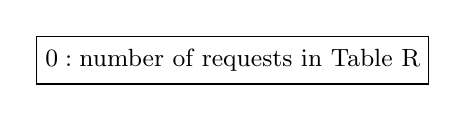
\begin{tikzpicture}
\small
\matrix[nodes={draw,minimum size=6mm}] {
  \node {$0:\textrm{number of requests in Table R}$};\\
};
\end{tikzpicture}\\
\textbf{Side Effects:} none.\\
\textbf{Throws:} {\tt{}SQLException} if database failure is encountered.\\
\bottomrule
\end{tabular}
\nwenddocs{}\nwbegincode{183}\sublabel{NW27XAxz-3rXeYk-1}\nwmargintag{{\nwtagstyle{}\subpageref{NW27XAxz-3rXeYk-1}}}\moddef{Query count of requests~{\nwtagstyle{}\subpageref{NW27XAxz-3rXeYk-1}}}\endmoddef\nwused{\\{NW27XAxz-4PbjF-1}}
public int[] DBQueryCountRequests() throws SQLException \{
  try (\LA{}Open \code{}conn\edoc{}~{\nwtagstyle{}\subpageref{NW27XAxz-JT1v9-1}}\RA{}) \{
    return this.DBFetch(conn, "S67", 1);
  \} catch (SQLException e) \{
    throw e;
  \}
\}
\nwindexdefn{DBQueryCountRequests}{DBQueryCountRequests}{NW27XAxz-3rXeYk-1}\eatline
\nwidentdefs{\\{{DBQueryCountRequests}{DBQueryCountRequests}}}\nwidentuses{\\{{DBFetch}{DBFetch}}\\{{S67}{S67}}}\nwindexuse{DBFetch}{DBFetch}{NW27XAxz-3rXeYk-1}\nwindexuse{S67}{S67}{NW27XAxz-3rXeYk-1}\nwendcode{}\nwbegindocs{184}\nwdocspar
\subsection{{\tt{}\protect\nwindexuse{DBQueryAllUsers}{DBQueryAllUsers}{NW27XAxz-3isdeu-1}DBQueryAllUsers}(0)}
\begin{tabular}{p{\textwidth}}
\toprule
\rowcolor{TableTitle}
Method \textcolor{blue}{{\tt{}\protect\nwindexuse{DBQueryAllUsers}{DBQueryAllUsers}{NW27XAxz-3isdeu-1}DBQueryAllUsers}}(0) returns all rows in view {\tt{}r{\char95}user}.
A {\tt{}SQLException} is thrown in case of database failure.\\
\midrule
\textbf{Parameters:} none.\\
\textbf{Returns:} results of the query flattened into an integer array, or
{\tt{}null} if no results.

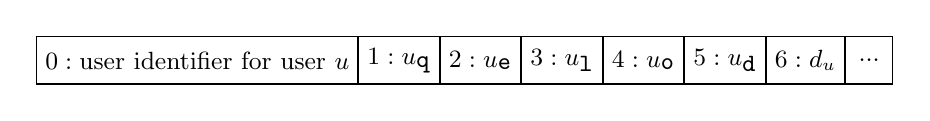
\begin{tikzpicture}
\small
\matrix[nodes={draw,minimum size=6mm}] {
  \node {$0:\textrm{user identifier for user $u$}$};
 &\node {$1:u_\texttt{q}$};
 &\node {$2:u_\texttt{e}$};
 &\node {$3:u_\texttt{l}$};
 &\node {$4:u_\texttt{o}$};
 &\node {$5:u_\texttt{d}$};
 &\node {$6:d_u$};
 &\node {...};\\
};
\end{tikzpicture}\\
\textbf{Side Effects:} none.\\
\textbf{Throws:} {\tt{}SQLException} if database failure is encountered.\\
\bottomrule
\end{tabular}
\nwenddocs{}\nwbegincode{185}\sublabel{NW27XAxz-3isdeu-1}\nwmargintag{{\nwtagstyle{}\subpageref{NW27XAxz-3isdeu-1}}}\moddef{Query ridesharing user~{\nwtagstyle{}\subpageref{NW27XAxz-3isdeu-1}}}\endmoddef\nwalsodefined{\\{NW27XAxz-3isdeu-2}\\{NW2ZDXo8-3isdeu-3}\\{NWvbkzY-3isdeu-4}}\nwused{\\{NW27XAxz-4PbjF-1}\\{NW2ZDXo8-bF3Hn-2}\\{NWvbkzY-3YjONp-3}}
public int[] DBQueryAllUsers() throws SQLException \{
  try (\LA{}Open \code{}conn\edoc{}~{\nwtagstyle{}\subpageref{NW27XAxz-JT1v9-1}}\RA{}) \{
    return this.DBFetch(conn, "S141", 7);
  \} catch (SQLException e) \{
    throw e;
  \}
\}
\nwindexdefn{DBQueryAllUsers}{DBQueryAllUsers}{NW27XAxz-3isdeu-1}\eatline
\nwidentdefs{\\{{DBQueryAllUsers}{DBQueryAllUsers}}}\nwidentuses{\\{{DBFetch}{DBFetch}}\\{{S141}{S141}}}\nwindexuse{DBFetch}{DBFetch}{NW27XAxz-3isdeu-1}\nwindexuse{S141}{S141}{NW27XAxz-3isdeu-1}\nwendcode{}\nwbegindocs{186}\nwdocspar
\subsection{{\tt{}\protect\nwindexuse{DBQueryUser}{DBQueryUser}{NW27XAxz-3isdeu-2}DBQueryUser}(1)}
\begin{tabular}{p{\textwidth}}
\toprule
\rowcolor{TableTitle}
Method \textcolor{blue}{{\tt{}\protect\nwindexuse{DBQueryUser}{DBQueryUser}{NW27XAxz-3isdeu-2}DBQueryUser}}(0) returns the properties of the
given user.
A {\tt{}UserNotFoundException} is thrown if the user does not exist.\\
\midrule
\textbf{Parameters:} \\
\begin{tabular}{lp{116mm}}
Integer {\tt{}uid} (param. 1):&user identifier for user $u$
\end{tabular}
\textbf{Returns:} results of the query flattened into an integer array, or
{\tt{}null} if no results.

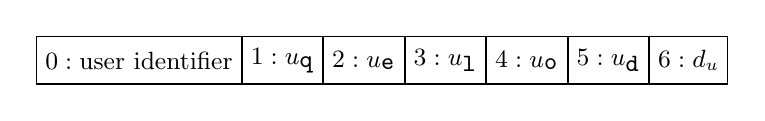
\begin{tikzpicture}
\small
\matrix[nodes={draw,minimum size=6mm}] {
  \node {$0:\textrm{user identifier}$};
 &\node {$1:u_\texttt{q}$};
 &\node {$2:u_\texttt{e}$};
 &\node {$3:u_\texttt{l}$};
 &\node {$4:u_\texttt{o}$};
 &\node {$5:u_\texttt{d}$};
 &\node {$6:d_u$};\\
};
\end{tikzpicture}\\
\textbf{Side Effects:} none.\\
\textbf{Throws:} {\tt{}UserNotFoundException} if user does not exist.\\
\bottomrule
\end{tabular}
\nwenddocs{}\nwbegincode{187}\sublabel{NW27XAxz-3isdeu-2}\nwmargintag{{\nwtagstyle{}\subpageref{NW27XAxz-3isdeu-2}}}\moddef{Query ridesharing user~{\nwtagstyle{}\subpageref{NW27XAxz-3isdeu-1}}}\plusendmoddef
public int[] DBQueryUser(final int uid)
throws UserNotFoundException \{
  if (!this.lu_users.containsKey(uid)) \{
    throw new UserNotFoundException("User "+uid+" not found.");
  \}
  return this.lu_users.get(uid).clone();
\}
\nwindexdefn{DBQueryUser}{DBQueryUser}{NW27XAxz-3isdeu-2}\eatline
\nwidentdefs{\\{{DBQueryUser}{DBQueryUser}}}\nwidentuses{\\{{lu{\char95}users}{lu:unusers}}}\nwindexuse{lu{\char95}users}{lu:unusers}{NW27XAxz-3isdeu-2}\nwendcode{}\nwbegindocs{188}\nwdocspar
\subsection{{\tt{}\protect\nwindexuse{DBQueryRequestStatus}{DBQueryRequestStatus}{NW27XAxz-1hFvVm-1}DBQueryRequestStatus}(2)}
\begin{tabular}{p{\textwidth}}
\toprule
\rowcolor{TableTitle}
Method \textcolor{blue}{{\tt{}\protect\nwindexuse{DBQueryRequestStatus}{DBQueryRequestStatus}{NW27XAxz-1hFvVm-1}DBQueryRequestStatus}}(0) returns the status of
the given request at the given time (Eq.~\ref{eq:status}).
A {\tt{}UserNotFoundException} is thrown if the user does not exist.
A {\tt{}SQLException} is thrown in case of database failure.\\
\midrule
\textbf{Parameters:} \\
\begin{tabular}{lp{116mm}}
Integer {\tt{}rid} (param. 1):&user identifier for request $r$\\
Integer {\tt{}t} (param. 2):&a time
\end{tabular}\\
\textbf{Returns:} results of the query flattened into an integer array, or
{\tt{}null} if no results.

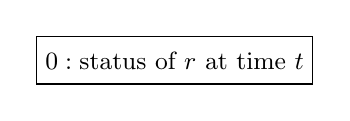
\begin{tikzpicture}
\small
\matrix[nodes={draw,minimum size=6mm}] {
  \node {$0:\textrm{status of $r$ at time $t$}$};\\
};
\end{tikzpicture}\\
\textbf{Side Effects:} none.\\
\textbf{Throws:} {\tt{}UserNotFoundException} if user does not exist, or
{\tt{}SQLException} if database failure is encountered.\\
\bottomrule
\end{tabular}
\nwenddocs{}\nwbegincode{189}\sublabel{NW27XAxz-1hFvVm-1}\nwmargintag{{\nwtagstyle{}\subpageref{NW27XAxz-1hFvVm-1}}}\moddef{Query request status~{\nwtagstyle{}\subpageref{NW27XAxz-1hFvVm-1}}}\endmoddef\nwused{\\{NW27XAxz-4PbjF-1}}
public int[] DBQueryRequestStatus(final int rid, final int t)
throws UserNotFoundException, SQLException \{
  if (!this.lu_users.containsKey(rid)) \{
    throw new UserNotFoundException("User "+rid+" not found.");
  \}
  try (\LA{}Open \code{}conn\edoc{}~{\nwtagstyle{}\subpageref{NW27XAxz-JT1v9-1}}\RA{}) \{
    return this.DBFetch(conn, "S133", 1, rid, t);
  \} catch (SQLException e) \{
    throw e;
  \}
\}
\nwindexdefn{DBQueryRequestStatus}{DBQueryRequestStatus}{NW27XAxz-1hFvVm-1}\eatline
\nwidentdefs{\\{{DBQueryRequestStatus}{DBQueryRequestStatus}}}\nwidentuses{\\{{DBFetch}{DBFetch}}\\{{lu{\char95}users}{lu:unusers}}\\{{S133}{S133}}}\nwindexuse{DBFetch}{DBFetch}{NW27XAxz-1hFvVm-1}\nwindexuse{lu{\char95}users}{lu:unusers}{NW27XAxz-1hFvVm-1}\nwindexuse{S133}{S133}{NW27XAxz-1hFvVm-1}\nwendcode{}\nwbegindocs{190}\nwdocspar
\subsection{{\tt{}\protect\nwindexuse{DBQueryRequestIsAssigned}{DBQueryRequestIsAssigned}{NW27XAxz-3k0aNo-1}DBQueryRequestIsAssigned}(1)}
\begin{tabular}{p{\textwidth}}
\toprule
\rowcolor{TableTitle}
Method \textcolor{blue}{{\tt{}\protect\nwindexuse{DBQueryRequestIsAssigned}{DBQueryRequestIsAssigned}{NW27XAxz-3k0aNo-1}DBQueryRequestIsAssigned}}(1) returns a
positive-length array if the given request is assigned (even if the request is
not yet picked-up), or {\tt{}null} if the request is not.  A
{\tt{}UserNotFoundException} is thrown if the user does not exist.
A {\tt{}SQLException} is thrown in case of database failure.\\
\midrule
\textbf{Parameters:} \\
\begin{tabular}{lp{116mm}}
Integer {\tt{}rid} (param. 1):&user identifier for request $r$
\end{tabular}\\
\textbf{Returns:} results of the query flattened into an integer array, or
{\tt{}null} if no results.

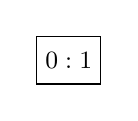
\begin{tikzpicture}
\small
\matrix[nodes={draw,minimum size=6mm}] {
  \node {$0:1$};\\
};
\end{tikzpicture}\\
\textbf{Side Effects:} none.\\
\textbf{Throws:} {\tt{}UserNotFoundException} if user does not exist, or
{\tt{}SQLException} if database failure is encountered.\\
\bottomrule
\end{tabular}
\nwenddocs{}\nwbegincode{191}\sublabel{NW27XAxz-3k0aNo-1}\nwmargintag{{\nwtagstyle{}\subpageref{NW27XAxz-3k0aNo-1}}}\moddef{Query request is assigned?~{\nwtagstyle{}\subpageref{NW27XAxz-3k0aNo-1}}}\endmoddef\nwused{\\{NW27XAxz-4PbjF-1}}
public int[] DBQueryRequestIsAssigned(final int rid) throws SQLException \{
  try (\LA{}Open \code{}conn\edoc{}~{\nwtagstyle{}\subpageref{NW27XAxz-JT1v9-1}}\RA{}) \{
    return this.DBFetch(conn, "S148", 1, rid);
  \} catch (SQLException e) \{
    throw e;
  \}
\}
\nwindexdefn{DBQueryRequestIsAssigned}{DBQueryRequestIsAssigned}{NW27XAxz-3k0aNo-1}\eatline
\nwidentdefs{\\{{DBQueryRequestIsAssigned}{DBQueryRequestIsAssigned}}}\nwidentuses{\\{{DBFetch}{DBFetch}}\\{{S148}{S148}}}\nwindexuse{DBFetch}{DBFetch}{NW27XAxz-3k0aNo-1}\nwindexuse{S148}{S148}{NW27XAxz-3k0aNo-1}\nwendcode{}\nwbegindocs{192}\nwdocspar
\subsection{{\tt{}\protect\nwindexuse{DBQueryQueuedRequests}{DBQueryQueuedRequests}{NW27XAxz-3AGrxZ-1}DBQueryQueuedRequests}(1)}
\begin{tabular}{p{\textwidth}}
\toprule
\rowcolor{TableTitle}
Method \textcolor{blue}{{\tt{}\protect\nwindexuse{DBQueryQueuedRequests}{DBQueryQueuedRequests}{NW27XAxz-3AGrxZ-1}DBQueryQueuedRequests}}(1) returns the requests
eligible for assignment at the given time. A request $r$ is ``eligible'' if it
is not assigned at the given time, and if the given time is between the
request's early time $r_\texttt{e}$ and
$(r_\texttt{e}+\texttt{REQUEST\_TIMEOUT})$.
A {\tt{}SQLException} is thrown in case of database failure.\\
\midrule
\textbf{Parameters:} \\
\begin{tabular}{lp{116mm}}
Integer {\tt{}t} (param. 1):&a time
\end{tabular}\\
\textbf{Returns:} results of the query flattened into an integer array, or
{\tt{}null} if no results.

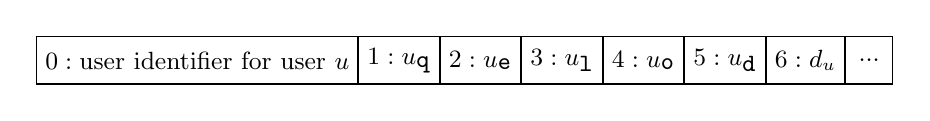
\begin{tikzpicture}
\small
\matrix[nodes={draw,minimum size=6mm}] {
  \node {$0:\textrm{user identifier for user $u$}$};
 &\node {$1:u_\texttt{q}$};
 &\node {$2:u_\texttt{e}$};
 &\node {$3:u_\texttt{l}$};
 &\node {$4:u_\texttt{o}$};
 &\node {$5:u_\texttt{d}$};
 &\node {$6:d_u$};
 &\node {...};\\
};
\end{tikzpicture}\\
\textbf{Side Effects:} none.\\
\textbf{Throws:} {\tt{}SQLException} if database failure is encountered.\\
\bottomrule
\end{tabular}
\nwenddocs{}\nwbegincode{193}\sublabel{NW27XAxz-3AGrxZ-1}\nwmargintag{{\nwtagstyle{}\subpageref{NW27XAxz-3AGrxZ-1}}}\moddef{Query queued requests~{\nwtagstyle{}\subpageref{NW27XAxz-3AGrxZ-1}}}\endmoddef\nwalsodefined{\\{NW27XAxz-3AGrxZ-2}\\{NW27XAxz-3AGrxZ-3}\\{NW2ZDXo8-3AGrxZ-4}}\nwused{\\{NW27XAxz-4PbjF-1}\\{NW2ZDXo8-bF3Hn-2}}
public int[] DBQueryQueuedRequests(final int t) throws SQLException \{
  try (\LA{}Open \code{}conn\edoc{}~{\nwtagstyle{}\subpageref{NW27XAxz-JT1v9-1}}\RA{}) \{
\nosublabel{NW27XAxz-3AGrxZ-1-u1}\nwindexdefn{DBQueryQueuedRequests}{DBQueryQueuedRequests}{NW27XAxz-3AGrxZ-1}\eatline
\nwidentdefs{\\{{DBQueryQueuedRequests}{DBQueryQueuedRequests}}}\nwendcode{}\nwbegindocs{194}{\small Our approach is to first select all requests where $t$ is between the
request's early time $r_\texttt{e}$ and
$r_\texttt{e}+\texttt{REQUEST\_TIMEOUT}$.  Then, we return a filtered subset of
these requests that are unassigned. As we don't know how many requests will
returned in the end, we initialize a temporary array {\tt{}temp1} to hold the
pre-filter number of requests.}
\nwenddocs{}\nwbegincode{195}\sublabel{NW27XAxz-3AGrxZ-2}\nwmargintag{{\nwtagstyle{}\subpageref{NW27XAxz-3AGrxZ-2}}}\moddef{Query queued requests~{\nwtagstyle{}\subpageref{NW27XAxz-3AGrxZ-1}}}\plusendmoddef
    final int[] output = this.DBFetch(conn, "S143", 7, t, t, REQUEST_TIMEOUT);
    int[] temp1 = new int[output.length];
    int j = 0;
    for (int i = 0; i < (output.length - 6); i += 7) \{
      if (this.lu_rstatus.get(output[i]) == false) \{
        temp1[(j + 0)] = output[(i + 0)];
        temp1[(j + 1)] = output[(i + 1)];
        temp1[(j + 2)] = output[(i + 2)];
        temp1[(j + 3)] = output[(i + 3)];
        temp1[(j + 4)] = output[(i + 4)];
        temp1[(j + 5)] = output[(i + 5)];
        temp1[(j + 6)] = output[(i + 6)];
        j += 7;
      \}
    \}
\nwidentuses{\\{{DBFetch}{DBFetch}}\\{{lu{\char95}rstatus}{lu:unrstatus}}\\{{REQUEST{\char95}TIMEOUT}{REQUEST:unTIMEOUT}}\\{{S143}{S143}}}\nwindexuse{DBFetch}{DBFetch}{NW27XAxz-3AGrxZ-2}\nwindexuse{lu{\char95}rstatus}{lu:unrstatus}{NW27XAxz-3AGrxZ-2}\nwindexuse{REQUEST{\char95}TIMEOUT}{REQUEST:unTIMEOUT}{NW27XAxz-3AGrxZ-2}\nwindexuse{S143}{S143}{NW27XAxz-3AGrxZ-2}\nwendcode{}\nwbegindocs{196}\nwdocspar
{\small We copy the non-null elements of {\tt{}temp1} into a second array
{\tt{}temp2} and return {\tt{}temp2}.}
\nwenddocs{}\nwbegincode{197}\sublabel{NW27XAxz-3AGrxZ-3}\nwmargintag{{\nwtagstyle{}\subpageref{NW27XAxz-3AGrxZ-3}}}\moddef{Query queued requests~{\nwtagstyle{}\subpageref{NW27XAxz-3AGrxZ-1}}}\plusendmoddef
    int[] temp2 = new int[j];
    for (int i = 0; i < j; i += 7) \{
      temp2[(i + 0)] = temp1[(i + 0)];
      temp2[(i + 1)] = temp1[(i + 1)];
      temp2[(i + 2)] = temp1[(i + 2)];
      temp2[(i + 3)] = temp1[(i + 3)];
      temp2[(i + 4)] = temp1[(i + 4)];
      temp2[(i + 5)] = temp1[(i + 5)];
      temp2[(i + 6)] = temp1[(i + 6)];
    \}
    return temp2;
  \} catch (SQLException e) \{
    throw e;
  \}
\}
\nwendcode{}\nwbegindocs{198}\nwdocspar

\subsection{{\tt{}\protect\nwindexuse{DBQueryActiveServers}{DBQueryActiveServers}{NW27XAxz-pt8I9-1}DBQueryActiveServers}(1)}
\begin{tabular}{p{\textwidth}}
\toprule
\rowcolor{TableTitle}
Method \textcolor{blue}{{\tt{}\protect\nwindexuse{DBQueryActiveServers}{DBQueryActiveServers}{NW27XAxz-pt8I9-1}DBQueryActiveServers}}(1) returns the identifiers
of the active servers at the given time. A server is ``active'' if its
service has not ended.
A {\tt{}SQLException} is thrown in case of database failure.\\
\midrule
\textbf{Parameters:} \\
\begin{tabular}{lp{116mm}}
Integer {\tt{}t} (param. 1):&a time
\end{tabular}\\
\textbf{Returns:} results of the query flattened into an integer array, or
{\tt{}null} if no results.

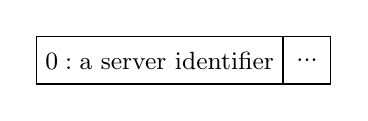
\begin{tikzpicture}
\small
\matrix[nodes={draw,minimum size=6mm}] {
  \node {$0:\textrm{a server identifier}$};
 &\node {...};\\
};
\end{tikzpicture}\\
\textbf{Side Effects:} none.\\
\textbf{Throws:} {\tt{}SQLException} if database failure is encountered.\\
\bottomrule
\end{tabular}
\nwenddocs{}\nwbegincode{199}\sublabel{NW27XAxz-pt8I9-1}\nwmargintag{{\nwtagstyle{}\subpageref{NW27XAxz-pt8I9-1}}}\moddef{Query active servers~{\nwtagstyle{}\subpageref{NW27XAxz-pt8I9-1}}}\endmoddef\nwused{\\{NW27XAxz-4PbjF-1}}
public int[] DBQueryActiveServers(final int t) throws SQLException \{
  try (\LA{}Open \code{}conn\edoc{}~{\nwtagstyle{}\subpageref{NW27XAxz-JT1v9-1}}\RA{}) \{
    return this.DBFetch(conn, "S134", 1, t, t, t);
  \} catch (SQLException e) \{
    throw e;
  \}
\}
\nwindexdefn{DBQueryActiveServers}{DBQueryActiveServers}{NW27XAxz-pt8I9-1}\eatline
\nwidentdefs{\\{{DBQueryActiveServers}{DBQueryActiveServers}}}\nwidentuses{\\{{DBFetch}{DBFetch}}\\{{S134}{S134}}}\nwindexuse{DBFetch}{DBFetch}{NW27XAxz-pt8I9-1}\nwindexuse{S134}{S134}{NW27XAxz-pt8I9-1}\nwendcode{}\nwbegindocs{200}\nwdocspar
\subsection{{\tt{}\protect\nwindexuse{DBQueryServerLocationsAll}{DBQueryServerLocationsAll}{NW27XAxz-rvb17-1}DBQueryServerLocationsAll}(1)}
\begin{tabular}{p{\textwidth}}
\toprule
\rowcolor{TableTitle}
Method \textcolor{blue}{{\tt{}\protect\nwindexuse{DBQueryServerLocationsAll}{DBQueryServerLocationsAll}{NW27XAxz-rvb17-1}DBQueryServerLocationsAll}}(1) returns the
last-known locations of all servers (including inactive servers) at the given
time. The ``last-known location'' is the waypoint in the server's route $w$
with a time component closest to but not exceeding the given time, in other
words ${w_{\leq t}}_{|w_{\leq t}|}$.
A {\tt{}SQLException} is thrown in case of database failure.\\
\midrule
\textbf{Parameters:} \\
\begin{tabular}{lp{116mm}}
Integer {\tt{}t} (param. 1):&a time
\end{tabular}\\
\textbf{Returns:} results of the query flattened into an integer array, or
{\tt{}null} if no results.

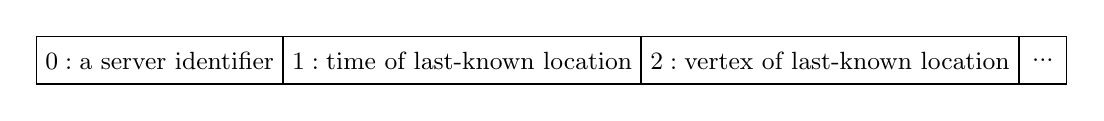
\begin{tikzpicture}
\small
\matrix[nodes={draw,minimum size=6mm}] {
  \node {$0:\textrm{a server identifier}$};
 &\node {$1:\textrm{time of last-known location}$};
 &\node {$2:\textrm{vertex of last-known location}$};
 &\node {...};\\
};
\end{tikzpicture}\\
\textbf{Side Effects:} none.\\
\textbf{Throws:} {\tt{}SQLException} if database failure is encountered.\\
\bottomrule
\end{tabular}
\nwenddocs{}\nwbegincode{201}\sublabel{NW27XAxz-rvb17-1}\nwmargintag{{\nwtagstyle{}\subpageref{NW27XAxz-rvb17-1}}}\moddef{Query all server locations~{\nwtagstyle{}\subpageref{NW27XAxz-rvb17-1}}}\endmoddef\nwused{\\{NW27XAxz-4PbjF-1}}
public int[] DBQueryServerLocationsAll(final int t) throws SQLException \{
  try (\LA{}Open \code{}conn\edoc{}~{\nwtagstyle{}\subpageref{NW27XAxz-JT1v9-1}}\RA{}) \{
    return this.DBFetch(conn, "S59", 3, t, t, t, t);
  \} catch (SQLException e) \{
    throw e;
  \}
\}
\nwindexdefn{DBQueryServerLocationsAll}{DBQueryServerLocationsAll}{NW27XAxz-rvb17-1}\eatline
\nwidentdefs{\\{{DBQueryServerLocationsAll}{DBQueryServerLocationsAll}}}\nwidentuses{\\{{DBFetch}{DBFetch}}\\{{S59}{S59}}}\nwindexuse{DBFetch}{DBFetch}{NW27XAxz-rvb17-1}\nwindexuse{S59}{S59}{NW27XAxz-rvb17-1}\nwendcode{}\nwbegindocs{202}\nwdocspar
\subsection{{\tt{}\protect\nwindexuse{DBQueryServerLocationsActive}{DBQueryServerLocationsActive}{NW27XAxz-3UaQCb-1}DBQueryServerLocationsActive}(1)}
\begin{tabular}{p{\textwidth}}
\toprule
\rowcolor{TableTitle}
Method \textcolor{blue}{{\tt{}\protect\nwindexuse{DBQueryServerLocationsActive}{DBQueryServerLocationsActive}{NW27XAxz-3UaQCb-1}DBQueryServerLocationsActive}}(1) returns the
last-known locations of all active servers at the given time. A server is
``active'' if its service has not ended, in other words it has not arrived
at its own destination.
The ``last-known location'' is the waypoint in the server's route $w$
with a time component closest to but not exceeding the given time, in other
words ${w_{\leq t}}_{|w_{\leq t}|}$.
A {\tt{}SQLException} is thrown in case of database failure.\\
\midrule
\textbf{Parameters:} \\
\begin{tabular}{lp{116mm}}
Integer {\tt{}t} (param. 1):&a time
\end{tabular}\\
\textbf{Returns:} results of the query flattened into an integer array, or
{\tt{}null} if no results.

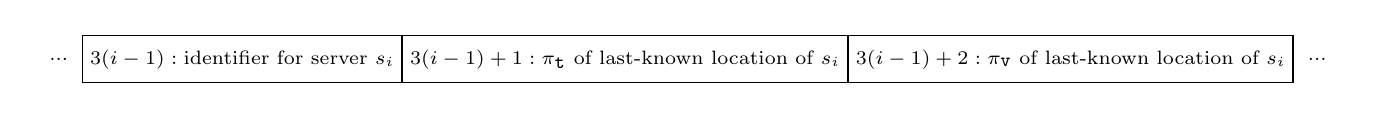
\begin{tikzpicture}
\scriptsize
\matrix[nodes={minimum size=6mm}] {
  \node {...};
 &\node[draw] {$3(i-1):\textrm{identifier for server $s_i$}$};
 &\node[draw] {$3(i-1)+1:\pi_\texttt{t}\textrm{ of last-known location of $s_i$}$};
 &\node[draw] {$3(i-1)+2:\pi_\texttt{v}\textrm{ of last-known location of $s_i$}$};
 &\node {...};\\
};
\end{tikzpicture}\\

where $1\leq i\leq |\mathcal{S}^\textrm{active}|$,
$s_i\in \mathcal{S}^\textrm{active}$, and
$\mathcal{S}^\textrm{active}= \{s\in\mathcal{S}\mid t^\textrm{arrive}(\mathcal{X},s)>t\}|$
for $t$ given by param. 1.\\
\textbf{Side Effects:} none.\\
\textbf{Throws:} {\tt{}SQLException} if database failure is encountered.\\
\bottomrule
\end{tabular}
\nwenddocs{}\nwbegincode{203}\sublabel{NW27XAxz-3UaQCb-1}\nwmargintag{{\nwtagstyle{}\subpageref{NW27XAxz-3UaQCb-1}}}\moddef{Query active server locations~{\nwtagstyle{}\subpageref{NW27XAxz-3UaQCb-1}}}\endmoddef\nwalsodefined{\\{NW27XAxz-3UaQCb-2}\\{NWvbkzY-3UaQCb-3}}\nwused{\\{NW27XAxz-4PbjF-1}\\{NWvbkzY-3YjONp-3}}
public int[] DBQueryServerLocationsActive(final int t) throws SQLException \{
  int[] output = new int[] \{ \};
  try (\LA{}Open \code{}conn\edoc{}~{\nwtagstyle{}\subpageref{NW27XAxz-JT1v9-1}}\RA{}) \{
    int j = 0;
\nosublabel{NW27XAxz-3UaQCb-1-u1}\nwindexdefn{DBQueryServerLocationsActive}{DBQueryServerLocationsActive}{NW27XAxz-3UaQCb-1}\eatline
\nwidentdefs{\\{{DBQueryServerLocationsActive}{DBQueryServerLocationsActive}}}\nwendcode{}\nwbegindocs{204}{\small Our approach is to first use statement {\tt{}\protect\nwindexuse{S134}{S134}{NW27XAxz-9eEGJ-1}S134} to get the active
servers. Then for each active server, we use either statement {\tt{}\protect\nwindexuse{S135}{S135}{NW27XAxz-4dp7jX-1}S135} or
{\tt{}\protect\nwindexuse{S147}{S147}{NW27XAxz-2TcddD-1}S147} to get its last-known location.}
\nwenddocs{}\nwbegincode{205}\sublabel{NW27XAxz-3UaQCb-2}\nwmargintag{{\nwtagstyle{}\subpageref{NW27XAxz-3UaQCb-2}}}\moddef{Query active server locations~{\nwtagstyle{}\subpageref{NW27XAxz-3UaQCb-1}}}\plusendmoddef
    final int[] temp1 = this.DBFetch(conn, "S134", 2, t, t, t);  // <-- 10 ms/call
    output = new int[(3*(temp1.length/2))];
    for (int i = 0; i < temp1.length - 1; i += 2) \{
      final int sid = temp1[(i + 0)];
      final int  te = temp1[(i + 1)];
      final int[] temp2 = (t < te
        ? this.DBFetch(conn, "S135", 2, sid, sid, t, t)  // <-- 0.07-0.15 ms/call
        : this.DBFetch(conn, "S147", 2, sid, sid));      // <-- 0.04-0.15 ms/call
      output[(j + 0)] = sid;
      output[(j + 1)] = temp2[0];
      output[(j + 2)] = temp2[1];
      j += 3;
    \}
  \} catch (SQLException e) \{
    throw e;
  \}
  return output;
\}
\nwidentuses{\\{{DBFetch}{DBFetch}}\\{{S134}{S134}}\\{{S135}{S135}}\\{{S147}{S147}}}\nwindexuse{DBFetch}{DBFetch}{NW27XAxz-3UaQCb-2}\nwindexuse{S134}{S134}{NW27XAxz-3UaQCb-2}\nwindexuse{S135}{S135}{NW27XAxz-3UaQCb-2}\nwindexuse{S147}{S147}{NW27XAxz-3UaQCb-2}\nwendcode{}\nwbegindocs{206}\nwdocspar

\subsection{{\tt{}\protect\nwindexuse{DBQueryServerRoute}{DBQueryServerRoute}{NW27XAxz-1AprqI-1}DBQueryServerRoute}(1)}
\begin{tabular}{p{\textwidth}}
\toprule
\rowcolor{TableTitle}
Method \textcolor{blue}{{\tt{}\protect\nwindexuse{DBQueryServerRoute}{DBQueryServerRoute}{NW27XAxz-1AprqI-1}DBQueryServerRoute}}(1) returns the route for the
given server identified by {\tt{}sid} (param. 1) at time $t$ (param. 2).
A {\tt{}SQLException} is thrown in case of database failure.\\
\midrule
\textbf{Parameters:} \\
\begin{tabular}{lp{116mm}}
Integer {\tt{}sid} (param. 1):&server identifier.\\
\end{tabular}
\textbf{Returns:} results of the query flattened into an integer array,
or {\tt{}null} if no results.

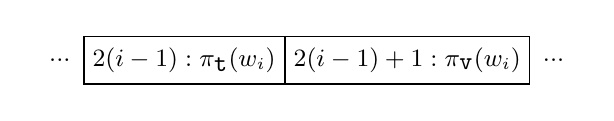
\begin{tikzpicture}
\small
\matrix[nodes={minimum size=6mm}] {
  \node {...};
 &\node[draw] {$2(i-1):\pi_\texttt{t}(w_i)$};
 &\node[draw] {$2(i-1)+1:\pi_\texttt{v}(w_i)$};
 &\node {...};\\
};
\end{tikzpicture}

where $1\leq i\leq |w|$ and $w$ is the route for the given server
identified by {\tt{}sid} (param. 1).\\
\textbf{Side Effects:} none.\\
\textbf{Throws:} {\tt{}SQLException} if database failure is encountered.\\
\bottomrule
\end{tabular}
\nwenddocs{}\nwbegincode{207}\sublabel{NW27XAxz-1AprqI-1}\nwmargintag{{\nwtagstyle{}\subpageref{NW27XAxz-1AprqI-1}}}\moddef{Query routes~{\nwtagstyle{}\subpageref{NW27XAxz-1AprqI-1}}}\endmoddef\nwalsodefined{\\{NW2ZDXo8-1AprqI-2}\\{NWvbkzY-1AprqI-3}}\nwused{\\{NW27XAxz-4PbjF-1}\\{NW2ZDXo8-bF3Hn-2}\\{NWvbkzY-3YjONp-3}}
public int[] DBQueryServerRoute(final int sid) throws SQLException \{
  try (\LA{}Open \code{}conn\edoc{}~{\nwtagstyle{}\subpageref{NW27XAxz-JT1v9-1}}\RA{}) \{
    return DBFetch(conn, "S60", 2, sid);
  \} catch (SQLException e) \{
    throw e;
  \}
\}
\nwindexdefn{DBQueryServerRoute}{DBQueryServerRoute}{NW27XAxz-1AprqI-1}\eatline
\nwidentdefs{\\{{DBQueryServerRoute}{DBQueryServerRoute}}}\nwidentuses{\\{{DBFetch}{DBFetch}}\\{{S60}{S60}}}\nwindexuse{DBFetch}{DBFetch}{NW27XAxz-1AprqI-1}\nwindexuse{S60}{S60}{NW27XAxz-1AprqI-1}\nwendcode{}\nwbegindocs{208}\nwdocspar
\subsection{{\tt{}\protect\nwindexuse{DBQueryServerSchedule}{DBQueryServerSchedule}{NW27XAxz-3yA8FQ-1}DBQueryServerSchedule}(1)}
\begin{tabular}{p{\textwidth}}
\toprule
\rowcolor{TableTitle}
Method \textcolor{blue}{{\tt{}\protect\nwindexuse{DBQueryServerSchedule}{DBQueryServerSchedule}{NW27XAxz-3yA8FQ-1}DBQueryServerSchedule}}(1) returns the schedule
for the given server.
A {\tt{}SQLException} is thrown in case of database failure.\\
\midrule
\textbf{Parameters:} \\
\begin{tabular}{lp{116mm}}
Integer {\tt{}sid} (param. 1):&server identifier.\\
\end{tabular}
\textbf{Returns:} results of the query flattened into an integer array,
or {\tt{}null} if no results.

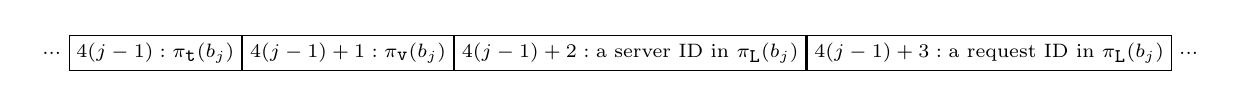
\begin{tikzpicture}
\scriptsize
\matrix[nodes={}] {
  \node {...};
 &\node[draw] {$4(j-1):\pi_\texttt{t}(b_j)$};
 &\node[draw] {$4(j-1)+1:\pi_\texttt{v}(b_j)$};
 &\node[draw] {$4(j-1)+2:\textrm{a server ID in }\pi_\texttt{L}(b_j)$};
 &\node[draw] {$4(j-1)+3:\textrm{a request ID in }\pi_\texttt{L}(b_j)$};
 &\node {...};\\
};
\end{tikzpicture}

where $1\leq j\leq |b|$ and $b$ is the schedule for the
given server  identified by {\tt{}sid} (param. 1).
If a label is empty (\textit{e.g.} not all waypoints will have a server
identifier in their label set), the element will be 0. If a waypoint has
multiple labels, the waypoint will be written once for each of the labels.
The returned sequence is in time-ascending order but \textbf{is not guaranteed}
to be in the same order as the actual pick-ups and drop-offs, \textit{e.g.} if a
waypoint has multiple labels with some indicating pick-ups and some indicating
drop-offs, the ordering of these waypoints is uncertain.\\
\textbf{Side Effects:} none.\\
\textbf{Throws:} {\tt{}SQLException} if database failure is encountered.\\
\bottomrule
\end{tabular}
\nwenddocs{}\nwbegincode{209}\sublabel{NW27XAxz-3yA8FQ-1}\nwmargintag{{\nwtagstyle{}\subpageref{NW27XAxz-3yA8FQ-1}}}\moddef{Query schedules~{\nwtagstyle{}\subpageref{NW27XAxz-3yA8FQ-1}}}\endmoddef\nwalsodefined{\\{NW2ZDXo8-3yA8FQ-2}\\{NWvbkzY-3yA8FQ-3}}\nwused{\\{NW27XAxz-4PbjF-1}\\{NW2ZDXo8-bF3Hn-2}\\{NWvbkzY-3YjONp-3}}
public int[] DBQueryServerSchedule(final int sid) throws SQLException \{
  try (\LA{}Open \code{}conn\edoc{}~{\nwtagstyle{}\subpageref{NW27XAxz-JT1v9-1}}\RA{}) \{
    return DBFetch(conn, "S61", 4, sid);
  \} catch (SQLException e) \{
    throw e;
  \}
\}
\nwindexdefn{DBQueryServerSchedule}{DBQueryServerSchedule}{NW27XAxz-3yA8FQ-1}\eatline
\nwidentdefs{\\{{DBQueryServerSchedule}{DBQueryServerSchedule}}}\nwidentuses{\\{{DBFetch}{DBFetch}}\\{{S61}{S61}}}\nwindexuse{DBFetch}{DBFetch}{NW27XAxz-3yA8FQ-1}\nwindexuse{S61}{S61}{NW27XAxz-3yA8FQ-1}\nwendcode{}\nwbegindocs{210}\nwdocspar
\subsection{{\tt{}\protect\nwindexuse{DBQueryServerRemainingRoute}{DBQueryServerRemainingRoute}{NW27XAxz-23oLro-1}DBQueryServerRemainingRoute}(2)}
\begin{tabular}{p{\textwidth}}
\toprule
\rowcolor{TableTitle}
Method \textcolor{blue}{{\tt{}\protect\nwindexuse{DBQueryServerRemainingRoute}{DBQueryServerRemainingRoute}{NW27XAxz-23oLro-1}DBQueryServerRemainingRoute}}(2) returns the
remaining route for the given server at the given time.
A {\tt{}SQLException} is thrown in case of database failure.\\
\midrule
\textbf{Parameters:} \\
\begin{tabular}{lp{116mm}}
Integer {\tt{}sid} (param. 1):&server identifier.\\
Integer {\tt{}t} (param. 2):&a time.\\
\end{tabular}
\textbf{Returns:} results of the query flattened into an integer array,
or {\tt{}null} if no results.

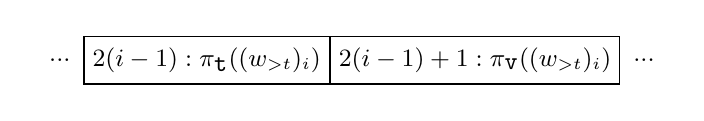
\begin{tikzpicture}
\small
\matrix[nodes={minimum size=6mm}] {
  \node {...};
 &\node[draw] {$2(i-1):\pi_\texttt{t}({(w_{>t}})_i)$};
 &\node[draw] {$2(i-1)+1:\pi_\texttt{v}({(w_{>t}})_i)$};
 &\node {...};\\
};
\end{tikzpicture}

where $1\leq i\leq |w_{>t}|$ and $w_{>t}$ is the remaining route for the
given server identified by {\tt{}sid} (param. 1) at time $t$ (param. 2).\\
\textbf{Side Effects:} none.\\
\textbf{Throws:} {\tt{}SQLException} if database failure is encountered.\\
\bottomrule
\end{tabular}
\nwenddocs{}\nwbegincode{211}\sublabel{NW27XAxz-23oLro-1}\nwmargintag{{\nwtagstyle{}\subpageref{NW27XAxz-23oLro-1}}}\moddef{Query remaining routes~{\nwtagstyle{}\subpageref{NW27XAxz-23oLro-1}}}\endmoddef\nwused{\\{NW27XAxz-4PbjF-1}}
public int[] DBQueryServerRemainingRoute(final int sid, final int t) throws SQLException \{
  try (\LA{}Open \code{}conn\edoc{}~{\nwtagstyle{}\subpageref{NW27XAxz-JT1v9-1}}\RA{}) \{
    return DBFetch(conn, "S129", 2, sid, t);
  \} catch (SQLException e) \{
    throw e;
  \}
\}
\nwindexdefn{DBQueryServerRemainingRoute}{DBQueryServerRemainingRoute}{NW27XAxz-23oLro-1}\eatline
\nwidentdefs{\\{{DBQueryServerRemainingRoute}{DBQueryServerRemainingRoute}}}\nwidentuses{\\{{DBFetch}{DBFetch}}\\{{S129}{S129}}}\nwindexuse{DBFetch}{DBFetch}{NW27XAxz-23oLro-1}\nwindexuse{S129}{S129}{NW27XAxz-23oLro-1}\nwendcode{}\nwbegindocs{212}\nwdocspar
\subsection{{\tt{}\protect\nwindexuse{DBQueryServerRemainingSchedule}{DBQueryServerRemainingSchedule}{NW27XAxz-1oPNKc-1}DBQueryServerRemainingSchedule}(2)}
\begin{tabular}{p{\textwidth}}
\toprule
\rowcolor{TableTitle}
Method \textcolor{blue}{{\tt{}\protect\nwindexuse{DBQueryServerRemainingSchedule}{DBQueryServerRemainingSchedule}{NW27XAxz-1oPNKc-1}DBQueryServerRemainingSchedule}}(2) returns the
remaining schedule for the given server at the given time.
A {\tt{}SQLException} is thrown in case of database failure.\\
\midrule
\textbf{Parameters:} \\
\begin{tabular}{lp{116mm}}
Integer {\tt{}sid} (param. 1):&server identifier.\\
Integer {\tt{}t} (param. 2):&a time.\\
\end{tabular}
\textbf{Returns:} results of the query flattened into an integer array,
or {\tt{}null} if no results.

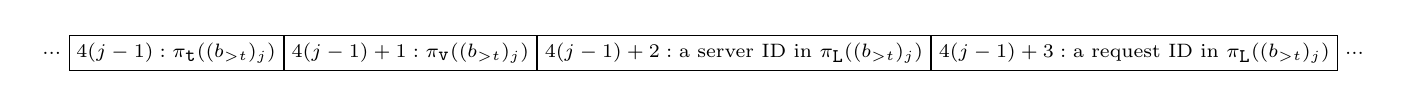
\begin{tikzpicture}
\scriptsize
\matrix[nodes={}] {
  \node {...};
 &\node[draw] {$4(j-1):\pi_\texttt{t}((b_{>t})_j)$};
 &\node[draw] {$4(j-1)+1:\pi_\texttt{v}((b_{>t})_j)$};
 &\node[draw] {$4(j-1)+2:\textrm{a server ID in }\pi_\texttt{L}((b_{>t})_j)$};
 &\node[draw] {$4(j-1)+3:\textrm{a request ID in }\pi_\texttt{L}((b_{>t})_j)$};
 &\node {...};\\
};
\end{tikzpicture}

where $1\leq j\leq |b_{>t}|$ and $b_{>t}$ is the remaining schedule for the
given server identified by {\tt{}sid} (param. 1) at time $t$ (param. 2).
If a label is empty (\textit{e.g.} not all waypoints will have a server
identifier in their label set), the element will be 0. If a waypoint has
multiple labels, the waypoint will be written once for each of the labels.
The returned sequence is in time-ascending order and \textbf{is guaranteed}
to be in the same order as the actual pick-ups and drop-offs.\\
\textbf{Side Effects:} none.\\
\textbf{Throws:} {\tt{}SQLException} if database failure is encountered.\\
\bottomrule
\end{tabular}
\nwenddocs{}\nwbegincode{213}\sublabel{NW27XAxz-1oPNKc-1}\nwmargintag{{\nwtagstyle{}\subpageref{NW27XAxz-1oPNKc-1}}}\moddef{Query remaining schedules~{\nwtagstyle{}\subpageref{NW27XAxz-1oPNKc-1}}}\endmoddef\nwused{\\{NW27XAxz-4PbjF-1}}
public int[] DBQueryServerRemainingSchedule(final int sid, final int t)
throws SQLException \{
  int[] output = new int[] \{ \};
  try (\LA{}Open \code{}conn\edoc{}~{\nwtagstyle{}\subpageref{NW27XAxz-JT1v9-1}}\RA{}) \{
    int[] temp = DBFetch(conn, "S144", 3, sid, t);
    output = new int[(4*temp.length/3 + 4)];
    int j = 0;
    for (int i = 0; i < (temp.length - 2); i += 3) \{
      output[(j + 0)] = temp[(i + 0)];
      output[(j + 1)] = temp[(i + 1)];
      output[(j + 2)] = 0;
      output[(j + 3)] = temp[(i + 2)];
      j += 4;
    \}
    temp = DBFetch(conn, "S145", 2, sid);
    output[(j + 0)] = temp[0];
    output[(j + 1)] = temp[1];
    output[(j + 2)] = sid;
    output[(j + 3)] = 0;
  \} catch (SQLException e) \{
    throw e;
  \}
  return output;
\}
\nwindexdefn{DBQueryServerRemainingSchedule}{DBQueryServerRemainingSchedule}{NW27XAxz-1oPNKc-1}\eatline
\nwidentdefs{\\{{DBQueryServerRemainingSchedule}{DBQueryServerRemainingSchedule}}}\nwidentuses{\\{{DBFetch}{DBFetch}}\\{{S144}{S144}}\\{{S145}{S145}}}\nwindexuse{DBFetch}{DBFetch}{NW27XAxz-1oPNKc-1}\nwindexuse{S144}{S144}{NW27XAxz-1oPNKc-1}\nwindexuse{S145}{S145}{NW27XAxz-1oPNKc-1}\nwendcode{}\nwbegindocs{214}\nwdocspar
\subsection{{\tt{}\protect\nwindexuse{DBQueryServerRemainingDistance}{DBQueryServerRemainingDistance}{NW27XAxz-3tQic5-1}DBQueryServerRemainingDistance}(2)}
\begin{tabular}{p{\textwidth}}
\toprule
\rowcolor{TableTitle}
Method \textcolor{blue}{{\tt{}\protect\nwindexuse{DBQueryServerRemainingDistance}{DBQueryServerRemainingDistance}{NW27XAxz-3tQic5-1}DBQueryServerRemainingDistance}}(2) returns the
remaining distance $D(w_{>t})$ for the given server at the given time.
A {\tt{}SQLException} is thrown in case of database failure.\\
\midrule
\textbf{Parameters:} \\
\begin{tabular}{lp{116mm}}
Integer {\tt{}sid} (param. 1):&server identifier.\\
Integer {\tt{}t} (param. 2):&a time.\\
\end{tabular}
\textbf{Returns:} results of the query flattened into an integer array,
or {\tt{}null} if no results.

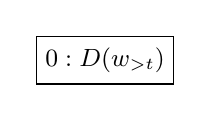
\begin{tikzpicture}
\small
\matrix[nodes={draw,minimum size=6mm}] {
  \node {$0:D(w_{>t})$};\\
};
\end{tikzpicture}

where $w_{>t}$ is the remaining route for the given server identified by {\tt{}sid} (param. 1).\\
\textbf{Side Effects:} none.\\
\textbf{Throws:} {\tt{}SQLException} if database failure is encountered.\\
\bottomrule
\end{tabular}
\nwenddocs{}\nwbegincode{215}\sublabel{NW27XAxz-3tQic5-1}\nwmargintag{{\nwtagstyle{}\subpageref{NW27XAxz-3tQic5-1}}}\moddef{Query remaining distance~{\nwtagstyle{}\subpageref{NW27XAxz-3tQic5-1}}}\endmoddef\nwalsodefined{\\{NWvbkzY-3tQic5-2}}\nwused{\\{NW27XAxz-4PbjF-1}\\{NWvbkzY-3YjONp-3}}
public int[] DBQueryServerRemainingDistance(final int sid, final int t)
throws SQLException \{
  try (\LA{}Open \code{}conn\edoc{}~{\nwtagstyle{}\subpageref{NW27XAxz-JT1v9-1}}\RA{}) \{
    return DBFetch(conn, "S142", 1, sid, t);
  \} catch (SQLException e) \{
    throw e;
  \}
\}
\nwindexdefn{DBQueryServerRemainingDistance}{DBQueryServerRemainingDistance}{NW27XAxz-3tQic5-1}\eatline
\nwidentdefs{\\{{DBQueryServerRemainingDistance}{DBQueryServerRemainingDistance}}}\nwidentuses{\\{{DBFetch}{DBFetch}}\\{{S142}{S142}}}\nwindexuse{DBFetch}{DBFetch}{NW27XAxz-3tQic5-1}\nwindexuse{S142}{S142}{NW27XAxz-3tQic5-1}\nwendcode{}\nwbegindocs{216}\nwdocspar
\subsection{{\tt{}\protect\nwindexuse{DBQueryServerRemainingDuration}{DBQueryServerRemainingDuration}{NW27XAxz-2cRw59-1}DBQueryServerRemainingDuration}(2)}
\begin{tabular}{p{\textwidth}}
\toprule
\rowcolor{TableTitle}
Method \textcolor{blue}{{\tt{}\protect\nwindexuse{DBQueryServerRemainingDuration}{DBQueryServerRemainingDuration}{NW27XAxz-2cRw59-1}DBQueryServerRemainingDuration}}(2) returns the
remaining duration $\delta(w_{>t})$ for the given server at the given time.
A {\tt{}SQLException} is thrown in case of database failure.\\
\midrule
\textbf{Parameters:} \\
\begin{tabular}{lp{116mm}}
Integer {\tt{}sid} (param. 1):&server identifier.\\
Integer {\tt{}t} (param. 2):&a time.\\
\end{tabular}
\textbf{Returns:} results of the query flattened into an integer array,
or {\tt{}null} if no results.

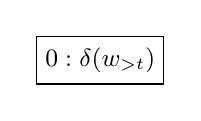
\begin{tikzpicture}
\small
\matrix[nodes={draw,minimum size=6mm}] {
  \node {$0:\delta(w_{>t})$};\\
};
\end{tikzpicture}

where $w_{>t}$ is the remaining route for the given server identified by {\tt{}sid} (param. 1).\\
\textbf{Side Effects:} none.\\
\textbf{Throws:} {\tt{}SQLException} if database failure is encountered.\\
\bottomrule
\end{tabular}
\nwenddocs{}\nwbegincode{217}\sublabel{NW27XAxz-2cRw59-1}\nwmargintag{{\nwtagstyle{}\subpageref{NW27XAxz-2cRw59-1}}}\moddef{Query remaining duration~{\nwtagstyle{}\subpageref{NW27XAxz-2cRw59-1}}}\endmoddef\nwalsodefined{\\{NWvbkzY-2cRw59-2}}\nwused{\\{NW27XAxz-4PbjF-1}\\{NWvbkzY-3YjONp-3}}
public int[] DBQueryServerRemainingDuration(final int sid, final int t)
throws SQLException \{
  try (\LA{}Open \code{}conn\edoc{}~{\nwtagstyle{}\subpageref{NW27XAxz-JT1v9-1}}\RA{}) \{
    int[] output = DBFetch(conn, "S127", 1, sid, t);
    if (output != null) \{
      output[0] -= t;
    \}
    return output;
  \} catch (SQLException e) \{
    throw e;
  \}
\}
\nwindexdefn{DBQueryServerRemainingDuration}{DBQueryServerRemainingDuration}{NW27XAxz-2cRw59-1}\eatline
\nwidentdefs{\\{{DBQueryServerRemainingDuration}{DBQueryServerRemainingDuration}}}\nwidentuses{\\{{DBFetch}{DBFetch}}\\{{S127}{S127}}}\nwindexuse{DBFetch}{DBFetch}{NW27XAxz-2cRw59-1}\nwindexuse{S127}{S127}{NW27XAxz-2cRw59-1}\nwendcode{}\nwbegindocs{218}\nwdocspar
\subsection{{\tt{}\protect\nwindexuse{DBQueryServerMaxLoad}{DBQueryServerMaxLoad}{NW27XAxz-3KLGqo-1}DBQueryServerMaxLoad}(2)}
\begin{tabular}{p{\textwidth}}
\toprule
\rowcolor{TableTitle}
Method \textcolor{blue}{{\tt{}\protect\nwindexuse{DBQueryServerMaxLoad}{DBQueryServerMaxLoad}{NW27XAxz-3KLGqo-1}DBQueryServerMaxLoad}}(2) returns the maximum load
for the given server at the given time. The ``maximum load'' is equal to the
load burden $Q(\mathcal{X},s,t)$ \emph{plus} the sum of the loads of the
requests that are dropped off by the server at $t$. In other words it is the
number of occupied seats at $t$ before any drop-offs happen.
A {\tt{}SQLException} is thrown in case of database failure.\\
\midrule
\textbf{Parameters:} \\
\begin{tabular}{lp{116mm}}
Integer {\tt{}sid} (param. 1):&server identifier.\\
Integer {\tt{}t} (param. 2):&a time.\\
\end{tabular}
\textbf{Returns:} results of the query flattened into an integer array,
or {\tt{}null} if no results.

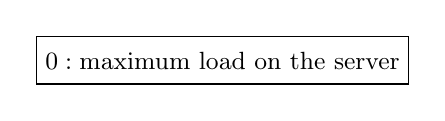
\begin{tikzpicture}
\small
\matrix[nodes={draw,minimum size=6mm}] {
  \node {$0:\textrm{maximum load on the server}$};\\
};
\end{tikzpicture}\\
\textbf{Side Effects:} none.\\
\textbf{Throws:} {\tt{}SQLException} if database failure is encountered.\\
\bottomrule
\end{tabular}
\nwenddocs{}\nwbegincode{219}\sublabel{NW27XAxz-3KLGqo-1}\nwmargintag{{\nwtagstyle{}\subpageref{NW27XAxz-3KLGqo-1}}}\moddef{Query max load~{\nwtagstyle{}\subpageref{NW27XAxz-3KLGqo-1}}}\endmoddef\nwalsodefined{\\{NWvbkzY-3KLGqo-2}}\nwused{\\{NW27XAxz-4PbjF-1}\\{NWvbkzY-3YjONp-3}}
public int[] DBQueryServerMaxLoad(final int sid, final int t) throws SQLException \{
  try (\LA{}Open \code{}conn\edoc{}~{\nwtagstyle{}\subpageref{NW27XAxz-JT1v9-1}}\RA{}) \{
    return DBFetch(conn, "S73", 1, sid, t);
  \} catch (SQLException e) \{
    throw e;
  \}
\}
\nwindexdefn{DBQueryServerMaxLoad}{DBQueryServerMaxLoad}{NW27XAxz-3KLGqo-1}\eatline
\nwidentdefs{\\{{DBQueryServerMaxLoad}{DBQueryServerMaxLoad}}}\nwidentuses{\\{{DBFetch}{DBFetch}}\\{{S73}{S73}}}\nwindexuse{DBFetch}{DBFetch}{NW27XAxz-3KLGqo-1}\nwindexuse{S73}{S73}{NW27XAxz-3KLGqo-1}\nwendcode{}\nwbegindocs{220}\nwdocspar
\subsection{{\tt{}\protect\nwindexuse{DBQueryServerPendingAssignments}{DBQueryServerPendingAssignments}{NW27XAxz-1UG2Ih-1}DBQueryServerPendingAssignments}(2)}
\begin{tabular}{p{\textwidth}}
\toprule
\rowcolor{TableTitle}
Method \textcolor{blue}{{\tt{}\protect\nwindexuse{DBQueryServerPendingAssignments}{DBQueryServerPendingAssignments}{NW27XAxz-1UG2Ih-1}DBQueryServerPendingAssignments}}(2) returns the
requests that will be picked up by the given server beyond the given time.
A {\tt{}SQLException} is thrown in case of database failure.\\
\midrule
\textbf{Parameters:} \\
\begin{tabular}{lp{116mm}}
Integer {\tt{}sid} (param. 1):&server identifier.\\
Integer {\tt{}t} (param. 2):&a time.\\
\end{tabular}
\textbf{Returns:} results of the query flattened into an integer array,
or {\tt{}null} if no results.

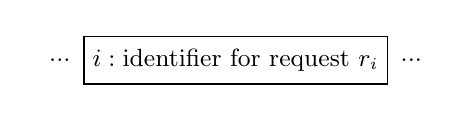
\begin{tikzpicture}
\small
\matrix[nodes={minimum size=6mm}] {
  \node {...};
 &\node[draw] {$i:\textrm{identifier for request }r_i$};
 &\node {...};\\
};
\end{tikzpicture}

where $1\leq i\leq |R^\textrm{pending}(\mathcal{X}, s, t)|$,
$r_i\in R^\textrm{pending}(\mathcal{X}, s, t)$, and
$R^\textrm{pending}(\mathcal{X}, s, t)= (R(\mathcal{X},s,H)\setminus R(\mathcal{X},s,t))$ for
time horizon $H$, server $s$ identified by {\tt{}sid} (param. 1), and time $t$ given by param. 2.\\
\textbf{Side Effects:} none.\\
\textbf{Throws:} {\tt{}SQLException} if database failure is encountered.\\
\bottomrule
\end{tabular}
\nwenddocs{}\nwbegincode{221}\sublabel{NW27XAxz-1UG2Ih-1}\nwmargintag{{\nwtagstyle{}\subpageref{NW27XAxz-1UG2Ih-1}}}\moddef{Query server pending assignments~{\nwtagstyle{}\subpageref{NW27XAxz-1UG2Ih-1}}}\endmoddef\nwused{\\{NW27XAxz-4PbjF-1}}
public int[] DBQueryServerPendingAssignments(final int sid, final int t)
throws SQLException \{
  try (\LA{}Open \code{}conn\edoc{}~{\nwtagstyle{}\subpageref{NW27XAxz-JT1v9-1}}\RA{}) \{
    return DBFetch(conn, "S100", 1, t, sid);
  \} catch (SQLException e) \{
    throw e;
  \}
\}
\nwindexdefn{DBQueryServerPendingAssignments}{DBQueryServerPendingAssignments}{NW27XAxz-1UG2Ih-1}\eatline
\nwidentdefs{\\{{DBQueryServerPendingAssignments}{DBQueryServerPendingAssignments}}}\nwidentuses{\\{{DBFetch}{DBFetch}}\\{{S100}{S100}}}\nwindexuse{DBFetch}{DBFetch}{NW27XAxz-1UG2Ih-1}\nwindexuse{S100}{S100}{NW27XAxz-1UG2Ih-1}\nwendcode{}\nwbegindocs{222}\nwdocspar
\subsection{{\tt{}\protect\nwindexuse{DBQueryServerCompletedAssignments}{DBQueryServerCompletedAssignments}{NW27XAxz-4CeViM-1}DBQueryServerCompletedAssignments}(2)}
\begin{tabular}{p{\textwidth}}
\toprule
\rowcolor{TableTitle}
Method \textcolor{blue}{{\tt{}\protect\nwindexuse{DBQueryServerCompletedAssignments}{DBQueryServerCompletedAssignments}{NW27XAxz-4CeViM-1}DBQueryServerCompletedAssignments}}(2) returns the
requests that have been dropped off by the given server on or before the given time,
in other words $R(\mathcal{X},s,t)$ (Eq.~\ref{eq:R(X,s,t)}).
A {\tt{}SQLException} is thrown in case of database failure.\\
\midrule
\textbf{Parameters:} \\
\begin{tabular}{lp{116mm}}
Integer {\tt{}sid} (param. 1):&server identifier.\\
Integer {\tt{}t} (param. 2):&a time.\\
\end{tabular}
\textbf{Returns:} results of the query flattened into an integer array,
or {\tt{}null} if no results.

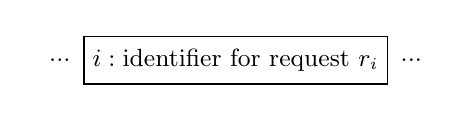
\begin{tikzpicture}
\small
\matrix[nodes={minimum size=6mm}] {
  \node {...};
 &\node[draw] {$i:\textrm{identifier for request }r_i$};
 &\node {...};\\
};
\end{tikzpicture}

where $1\leq i\leq |R(\mathcal{X},s,t)|$ and
$r_i\in R(\mathcal{X},s,t)$ for server $s$ identified by {\tt{}sid} (param. 1)
at time $t$ given by param. 2.\\
\textbf{Side Effects:} none.\\
\textbf{Throws:} {\tt{}SQLException} if database failure is encountered.\\
\bottomrule
\end{tabular}
\nwenddocs{}\nwbegincode{223}\sublabel{NW27XAxz-4CeViM-1}\nwmargintag{{\nwtagstyle{}\subpageref{NW27XAxz-4CeViM-1}}}\moddef{Query server completed assignments~{\nwtagstyle{}\subpageref{NW27XAxz-4CeViM-1}}}\endmoddef\nwused{\\{NW27XAxz-4PbjF-1}}
public int[] DBQueryServerCompletedAssignments(final int sid, final int t)
throws SQLException \{
  try (\LA{}Open \code{}conn\edoc{}~{\nwtagstyle{}\subpageref{NW27XAxz-JT1v9-1}}\RA{}) \{
    return DBFetch(conn, "S101", 1, t, sid);
  \} catch (SQLException e) \{
    throw e;
  \}
\}
\nwindexdefn{DBQueryServerCompletedAssignments}{DBQueryServerCompletedAssignments}{NW27XAxz-4CeViM-1}\eatline
\nwidentdefs{\\{{DBQueryServerCompletedAssignments}{DBQueryServerCompletedAssignments}}}\nwidentuses{\\{{DBFetch}{DBFetch}}\\{{S101}{S101}}}\nwindexuse{DBFetch}{DBFetch}{NW27XAxz-4CeViM-1}\nwindexuse{S101}{S101}{NW27XAxz-4CeViM-1}\nwendcode{}\nwbegindocs{224}\nwdocspar
\subsection{{\tt{}\protect\nwindexuse{DBQueryServiceRate}{DBQueryServiceRate}{NW27XAxz-1Ang64-1}DBQueryServiceRate}(0)}
\begin{tabular}{p{\textwidth}}
\toprule
\rowcolor{TableTitle}
Method \textcolor{blue}{{\tt{}\protect\nwindexuse{DBQueryServiceRate}{DBQueryServiceRate}{NW27XAxz-1Ang64-1}DBQueryServiceRate}}(0) returns the
service rate $\mu$ (Eq.~\ref{eq:service-rate}).
A {\tt{}SQLException} is thrown in case of database failure.\\
\midrule
\textbf{Parameters:} none.\\
\textbf{Returns:} results of the query flattened into an integer array,
or {\tt{}null} if no results.

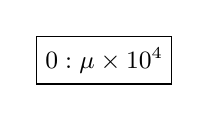
\begin{tikzpicture}
\small
\matrix[nodes={minimum size=6mm}] {
  \node[draw] {$0:\mu\times 10^4$};\\
};
\end{tikzpicture}

Note that the service rate is \textbf{multiplied by $10^4$} so that it can be
returned as an integer with 2 decimal points precision, for example if
$\mu=.1234$, then {\tt{}\protect\nwindexuse{DBQueryServiceRate}{DBQueryServiceRate}{NW27XAxz-1Ang64-1}DBQueryServiceRate}(0) returns $1234$.\\
\textbf{Side Effects:} none.\\
\textbf{Throws:} {\tt{}SQLException} if database failure is encountered.\\
\bottomrule
\end{tabular}
\nwenddocs{}\nwbegincode{225}\sublabel{NW27XAxz-1Ang64-1}\nwmargintag{{\nwtagstyle{}\subpageref{NW27XAxz-1Ang64-1}}}\moddef{Query various metrics~{\nwtagstyle{}\subpageref{NW27XAxz-1Ang64-1}}}\endmoddef\nwalsodefined{\\{NW27XAxz-1Ang64-2}\\{NW27XAxz-1Ang64-3}\\{NW27XAxz-1Ang64-4}\\{NW27XAxz-1Ang64-5}\\{NW27XAxz-1Ang64-6}\\{NW27XAxz-1Ang64-7}\\{NW27XAxz-1Ang64-8}\\{NW27XAxz-1Ang64-9}\\{NW27XAxz-1Ang64-A}\\{NW27XAxz-1Ang64-B}\\{NW27XAxz-1Ang64-C}\\{NW27XAxz-1Ang64-D}\\{NW27XAxz-1Ang64-E}\\{NW27XAxz-1Ang64-F}\\{NW27XAxz-1Ang64-G}\\{NW27XAxz-1Ang64-H}\\{NW27XAxz-1Ang64-I}\\{NW27XAxz-1Ang64-J}\\{NW27XAxz-1Ang64-K}\\{NW27XAxz-1Ang64-L}\\{NW27XAxz-1Ang64-M}\\{NW27XAxz-1Ang64-N}\\{NW27XAxz-1Ang64-O}\\{NW27XAxz-1Ang64-P}\\{NW27XAxz-1Ang64-Q}\\{NW27XAxz-1Ang64-R}\\{NW2ZDXo8-1Ang64-S}\\{NW2ZDXo8-1Ang64-T}\\{NW2ZDXo8-1Ang64-U}\\{NW2ZDXo8-1Ang64-V}\\{NW2ZDXo8-1Ang64-W}\\{NW2ZDXo8-1Ang64-X}\\{NW2ZDXo8-1Ang64-Y}\\{NW2ZDXo8-1Ang64-Z}\\{NW2ZDXo8-1Ang64-a}\\{NW2ZDXo8-1Ang64-b}\\{NW2ZDXo8-1Ang64-c}\\{NW2ZDXo8-1Ang64-d}\\{NW2ZDXo8-1Ang64-e}\\{NW2ZDXo8-1Ang64-f}\\{NW2ZDXo8-1Ang64-g}\\{NW2ZDXo8-1Ang64-h}\\{NW2ZDXo8-1Ang64-i}\\{NW2ZDXo8-1Ang64-j}\\{NW2ZDXo8-1Ang64-k}\\{NW2ZDXo8-1Ang64-l}\\{NW2ZDXo8-1Ang64-m}\\{NW2ZDXo8-1Ang64-n}\\{NW2ZDXo8-1Ang64-o}\\{NW2ZDXo8-1Ang64-p}}\nwused{\\{NW27XAxz-4PbjF-1}\\{NW2ZDXo8-bF3Hn-2}}
public int[] DBQueryServiceRate() throws SQLException \{
  try (\LA{}Open \code{}conn\edoc{}~{\nwtagstyle{}\subpageref{NW27XAxz-JT1v9-1}}\RA{}) \{
    return DBFetch(conn, "S102", 1);
  \} catch (SQLException e) \{
    throw e;
  \}
\}
\nwindexdefn{DBQueryServiceRate}{DBQueryServiceRate}{NW27XAxz-1Ang64-1}\eatline
\nwidentdefs{\\{{DBQueryServiceRate}{DBQueryServiceRate}}}\nwidentuses{\\{{DBFetch}{DBFetch}}\\{{S102}{S102}}}\nwindexuse{DBFetch}{DBFetch}{NW27XAxz-1Ang64-1}\nwindexuse{S102}{S102}{NW27XAxz-1Ang64-1}\nwendcode{}\nwbegindocs{226}\nwdocspar
\subsection{{\tt{}\protect\nwindexuse{DBQueryBaseDistanceTotal}{DBQueryBaseDistanceTotal}{NW27XAxz-1Ang64-2}DBQueryBaseDistanceTotal}(0)}
\begin{tabular}{p{\textwidth}}
\toprule
\rowcolor{TableTitle}
Method \textcolor{blue}{{\tt{}\protect\nwindexuse{DBQueryBaseDistanceTotal}{DBQueryBaseDistanceTotal}{NW27XAxz-1Ang64-2}DBQueryBaseDistanceTotal}}(0) returns the
base distance $D^\textrm{base}(\mathcal{U})$ (Eq.~\ref{eq:base-distance}).
A {\tt{}SQLException} is thrown in case of database failure.\\
\midrule
\textbf{Parameters:} none.\\
\textbf{Returns:} results of the query flattened into an integer array,
or {\tt{}null} if no results.

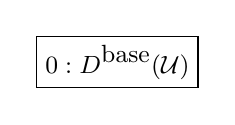
\begin{tikzpicture}
\small
\matrix[nodes={minimum size=6mm}] {
  \node[draw] {$0:D^\textrm{base}(\mathcal{U})$};\\
};
\end{tikzpicture}\\
\textbf{Side Effects:} none.\\
\textbf{Throws:} {\tt{}SQLException} if database failure is encountered.\\
\bottomrule
\end{tabular}
\nwenddocs{}\nwbegincode{227}\sublabel{NW27XAxz-1Ang64-2}\nwmargintag{{\nwtagstyle{}\subpageref{NW27XAxz-1Ang64-2}}}\moddef{Query various metrics~{\nwtagstyle{}\subpageref{NW27XAxz-1Ang64-1}}}\plusendmoddef
public int[] DBQueryBaseDistanceTotal() throws SQLException \{
  try (\LA{}Open \code{}conn\edoc{}~{\nwtagstyle{}\subpageref{NW27XAxz-JT1v9-1}}\RA{}) \{
    return DBFetch(conn, "S103", 1);
  \} catch (SQLException e) \{
    throw e;
  \}
\}
\nwindexdefn{DBQueryBaseDistanceTotal}{DBQueryBaseDistanceTotal}{NW27XAxz-1Ang64-2}\eatline
\nwidentdefs{\\{{DBQueryBaseDistanceTotal}{DBQueryBaseDistanceTotal}}}\nwidentuses{\\{{DBFetch}{DBFetch}}\\{{S103}{S103}}}\nwindexuse{DBFetch}{DBFetch}{NW27XAxz-1Ang64-2}\nwindexuse{S103}{S103}{NW27XAxz-1Ang64-2}\nwendcode{}\nwbegindocs{228}\nwdocspar
\subsection{{\tt{}\protect\nwindexuse{DBQueryServerBaseDistanceTotal}{DBQueryServerBaseDistanceTotal}{NW27XAxz-1Ang64-3}DBQueryServerBaseDistanceTotal}(0)}
\begin{tabular}{p{\textwidth}}
\toprule
\rowcolor{TableTitle}
Method \textcolor{blue}{{\tt{}\protect\nwindexuse{DBQueryServerBaseDistanceTotal}{DBQueryServerBaseDistanceTotal}{NW27XAxz-1Ang64-3}DBQueryServerBaseDistanceTotal}}(0) returns the
base distance of all the servers.
A {\tt{}SQLException} is thrown in case of database failure.\\
\midrule
\textbf{Parameters:} none.\\
\textbf{Returns:} results of the query flattened into an integer array,
or {\tt{}null} if no results.

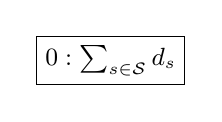
\begin{tikzpicture}
\small
\matrix[nodes={minimum size=6mm}] {
  \node[draw] {$0:\sum_{s\in\mathcal{S}}d_s$};\\
};
\end{tikzpicture}\\
\textbf{Side Effects:} none.\\
\textbf{Throws:} {\tt{}SQLException} if database failure is encountered.\\
\bottomrule
\end{tabular}
\nwenddocs{}\nwbegincode{229}\sublabel{NW27XAxz-1Ang64-3}\nwmargintag{{\nwtagstyle{}\subpageref{NW27XAxz-1Ang64-3}}}\moddef{Query various metrics~{\nwtagstyle{}\subpageref{NW27XAxz-1Ang64-1}}}\plusendmoddef
public int[] DBQueryServerBaseDistanceTotal() throws SQLException \{
  try (\LA{}Open \code{}conn\edoc{}~{\nwtagstyle{}\subpageref{NW27XAxz-JT1v9-1}}\RA{}) \{
    return DBFetch(conn, "S110", 1);
  \} catch (SQLException e) \{
    throw e;
  \}
\}
\nwindexdefn{DBQueryServerBaseDistanceTotal}{DBQueryServerBaseDistanceTotal}{NW27XAxz-1Ang64-3}\eatline
\nwidentdefs{\\{{DBQueryServerBaseDistanceTotal}{DBQueryServerBaseDistanceTotal}}}\nwidentuses{\\{{DBFetch}{DBFetch}}\\{{S110}{S110}}}\nwindexuse{DBFetch}{DBFetch}{NW27XAxz-1Ang64-3}\nwindexuse{S110}{S110}{NW27XAxz-1Ang64-3}\nwendcode{}\nwbegindocs{230}\nwdocspar
\subsection{{\tt{}\protect\nwindexuse{DBQueryRequestBaseDistanceTotal}{DBQueryRequestBaseDistanceTotal}{NW27XAxz-1Ang64-4}DBQueryRequestBaseDistanceTotal}(0)}
\begin{tabular}{p{\textwidth}}
\toprule
\rowcolor{TableTitle}
Method \textcolor{blue}{{\tt{}\protect\nwindexuse{DBQueryRequestBaseDistanceTotal}{DBQueryRequestBaseDistanceTotal}{NW27XAxz-1Ang64-4}DBQueryRequestBaseDistanceTotal}}(0) returns the
base distance of all the requests.
A {\tt{}SQLException} is thrown in case of database failure.\\
\midrule
\textbf{Parameters:} none.\\
\textbf{Returns:} results of the query flattened into an integer array,
or {\tt{}null} if no results.

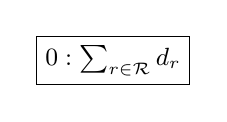
\begin{tikzpicture}
\small
\matrix[nodes={minimum size=6mm}] {
  \node[draw] {$0:\sum_{r\in\mathcal{R}}d_r$};\\
};
\end{tikzpicture}\\
\textbf{Side Effects:} none.\\
\textbf{Throws:} {\tt{}SQLException} if database failure is encountered.\\
\bottomrule
\end{tabular}
\nwenddocs{}\nwbegincode{231}\sublabel{NW27XAxz-1Ang64-4}\nwmargintag{{\nwtagstyle{}\subpageref{NW27XAxz-1Ang64-4}}}\moddef{Query various metrics~{\nwtagstyle{}\subpageref{NW27XAxz-1Ang64-1}}}\plusendmoddef
public int[] DBQueryRequestBaseDistanceTotal() throws SQLException \{
  try (\LA{}Open \code{}conn\edoc{}~{\nwtagstyle{}\subpageref{NW27XAxz-JT1v9-1}}\RA{}) \{
    return DBFetch(conn, "S111", 1);
  \} catch (SQLException e) \{
    throw e;
  \}
\}
\nwindexdefn{DBQueryRequestBaseDistanceTotal}{DBQueryRequestBaseDistanceTotal}{NW27XAxz-1Ang64-4}\eatline
\nwidentdefs{\\{{DBQueryRequestBaseDistanceTotal}{DBQueryRequestBaseDistanceTotal}}}\nwidentuses{\\{{DBFetch}{DBFetch}}\\{{S111}{S111}}}\nwindexuse{DBFetch}{DBFetch}{NW27XAxz-1Ang64-4}\nwindexuse{S111}{S111}{NW27XAxz-1Ang64-4}\nwendcode{}\nwbegindocs{232}\nwdocspar
\subsection{{\tt{}\protect\nwindexuse{DBQueryRequestBaseDistanceUnassigned}{DBQueryRequestBaseDistanceUnassigned}{NW27XAxz-1Ang64-5}DBQueryRequestBaseDistanceUnassigned}(0)}
\begin{tabular}{p{\textwidth}}
\toprule
\rowcolor{TableTitle}
Method \textcolor{blue}{{\tt{}\protect\nwindexuse{DBQueryRequestBaseDistanceUnassigned}{DBQueryRequestBaseDistanceUnassigned}{NW27XAxz-1Ang64-5}DBQueryRequestBaseDistanceUnassigned}}(0) returns the
base distance of all the unassigned requests.
A {\tt{}SQLException} is thrown in case of database failure.\\
\midrule
\textbf{Parameters:} none.\\
\textbf{Returns:} results of the query flattened into an integer array,
or {\tt{}null} if no results.

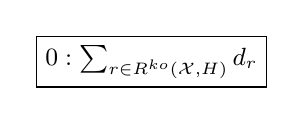
\begin{tikzpicture}
\small
\matrix[nodes={minimum size=6mm}] {
  \node[draw] {$0:\sum_{r\in R^{ko}(\mathcal{X},H)}d_r$};\\
};
\end{tikzpicture}

where $H$ is the time horizon.\\
\textbf{Side Effects:} none.\\
\textbf{Throws:} {\tt{}SQLException} if database failure is encountered.\\
\bottomrule
\end{tabular}
\nwenddocs{}\nwbegincode{233}\sublabel{NW27XAxz-1Ang64-5}\nwmargintag{{\nwtagstyle{}\subpageref{NW27XAxz-1Ang64-5}}}\moddef{Query various metrics~{\nwtagstyle{}\subpageref{NW27XAxz-1Ang64-1}}}\plusendmoddef
public int[] DBQueryRequestBaseDistanceUnassigned() throws SQLException \{
  try (\LA{}Open \code{}conn\edoc{}~{\nwtagstyle{}\subpageref{NW27XAxz-JT1v9-1}}\RA{}) \{
    return DBFetch(conn, "S138", 1);
  \} catch (SQLException e) \{
    throw e;
  \}
\}
\nwindexdefn{DBQueryRequestBaseDistanceUnassigned}{DBQueryRequestBaseDistanceUnassigned}{NW27XAxz-1Ang64-5}\eatline
\nwidentdefs{\\{{DBQueryRequestBaseDistanceUnassigned}{DBQueryRequestBaseDistanceUnassigned}}}\nwidentuses{\\{{DBFetch}{DBFetch}}\\{{S138}{S138}}}\nwindexuse{DBFetch}{DBFetch}{NW27XAxz-1Ang64-5}\nwindexuse{S138}{S138}{NW27XAxz-1Ang64-5}\nwendcode{}\nwbegindocs{234}\nwdocspar
\subsection{{\tt{}\protect\nwindexuse{DBQueryServerTravelDistance}{DBQueryServerTravelDistance}{NW27XAxz-1Ang64-6}DBQueryServerTravelDistance}(1)}
\begin{tabular}{p{\textwidth}}
\toprule
\rowcolor{TableTitle}
Method \textcolor{blue}{{\tt{}\protect\nwindexuse{DBQueryServerTravelDistance}{DBQueryServerTravelDistance}{NW27XAxz-1Ang64-6}DBQueryServerTravelDistance}}(1) returns the
travel distance $D(w)$ of the given server.
A {\tt{}SQLException} is thrown in case of database failure.\\
\midrule
\textbf{Parameters:} \\
\begin{tabular}{lp{116mm}}
Integer {\tt{}sid} (param. 1):&server identifier.
\end{tabular}\\
\textbf{Returns:} results of the query flattened into an integer array,
or {\tt{}null} if no results.

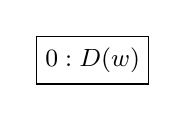
\begin{tikzpicture}
\small
\matrix[nodes={minimum size=6mm}] {
  \node[draw] {$0:D(w)$};\\
};
\end{tikzpicture}

where $w$ is the route of the given server identified by {\tt{}sid} (param. 1).\\
\textbf{Side Effects:} none.\\
\textbf{Throws:} {\tt{}SQLException} if database failure is encountered.\\
\bottomrule
\end{tabular}
\nwenddocs{}\nwbegincode{235}\sublabel{NW27XAxz-1Ang64-6}\nwmargintag{{\nwtagstyle{}\subpageref{NW27XAxz-1Ang64-6}}}\moddef{Query various metrics~{\nwtagstyle{}\subpageref{NW27XAxz-1Ang64-1}}}\plusendmoddef
public int[] DBQueryServerTravelDistance(final int sid) throws SQLException \{
  try (\LA{}Open \code{}conn\edoc{}~{\nwtagstyle{}\subpageref{NW27XAxz-JT1v9-1}}\RA{}) \{
    return DBFetch(conn, "S104", 1, sid);
  \} catch (SQLException e) \{
    throw e;
  \}
\}
\nwindexdefn{DBQueryServerTravelDistance}{DBQueryServerTravelDistance}{NW27XAxz-1Ang64-6}\eatline
\nwidentdefs{\\{{DBQueryServerTravelDistance}{DBQueryServerTravelDistance}}}\nwidentuses{\\{{DBFetch}{DBFetch}}\\{{S104}{S104}}}\nwindexuse{DBFetch}{DBFetch}{NW27XAxz-1Ang64-6}\nwindexuse{S104}{S104}{NW27XAxz-1Ang64-6}\nwendcode{}\nwbegindocs{236}\nwdocspar
\subsection{{\tt{}\protect\nwindexuse{DBQueryServerTravelDistanceTotal}{DBQueryServerTravelDistanceTotal}{NW27XAxz-1Ang64-7}DBQueryServerTravelDistanceTotal}(0)}
\begin{tabular}{p{\textwidth}}
\toprule
\rowcolor{TableTitle}
Method \textcolor{blue}{{\tt{}\protect\nwindexuse{DBQueryServerTravelDistanceTotal}{DBQueryServerTravelDistanceTotal}{NW27XAxz-1Ang64-7}DBQueryServerTravelDistanceTotal}}(0) returns the
total travel distance of all the servers.
A {\tt{}SQLException} is thrown in case of database failure.\\
\midrule
\textbf{Parameters:} none.\\
\textbf{Returns:} results of the query flattened into an integer array,
or {\tt{}null} if no results.

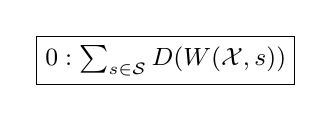
\begin{tikzpicture}
\small
\matrix[nodes={minimum size=6mm}] {
  \node[draw] {$0:\sum_{s\in\mathcal{S}}D(W(\mathcal{X},s))$};\\
};
\end{tikzpicture}\\
\textbf{Side Effects:} none.\\
\textbf{Throws:} {\tt{}SQLException} if database failure is encountered.\\
\bottomrule
\end{tabular}
\nwenddocs{}\nwbegincode{237}\sublabel{NW27XAxz-1Ang64-7}\nwmargintag{{\nwtagstyle{}\subpageref{NW27XAxz-1Ang64-7}}}\moddef{Query various metrics~{\nwtagstyle{}\subpageref{NW27XAxz-1Ang64-1}}}\plusendmoddef
public int[] DBQueryServerTravelDistanceTotal() throws SQLException \{
  try (\LA{}Open \code{}conn\edoc{}~{\nwtagstyle{}\subpageref{NW27XAxz-JT1v9-1}}\RA{}) \{
    return DBFetch(conn, "S105", 1);
  \} catch (SQLException e) \{
    throw e;
  \}
\}
\nwindexdefn{DBQueryServerTravelDistanceTotal}{DBQueryServerTravelDistanceTotal}{NW27XAxz-1Ang64-7}\eatline
\nwidentdefs{\\{{DBQueryServerTravelDistanceTotal}{DBQueryServerTravelDistanceTotal}}}\nwidentuses{\\{{DBFetch}{DBFetch}}\\{{S105}{S105}}}\nwindexuse{DBFetch}{DBFetch}{NW27XAxz-1Ang64-7}\nwindexuse{S105}{S105}{NW27XAxz-1Ang64-7}\nwendcode{}\nwbegindocs{238}\nwdocspar
\subsection{{\tt{}\protect\nwindexuse{DBQueryServerCruisingDistance}{DBQueryServerCruisingDistance}{NW27XAxz-1Ang64-8}DBQueryServerCruisingDistance}(1)}
\begin{tabular}{p{\textwidth}}
\toprule
\rowcolor{TableTitle}
Method \textcolor{blue}{{\tt{}\protect\nwindexuse{DBQueryServerCruisingDistance}{DBQueryServerCruisingDistance}{NW27XAxz-1Ang64-8}DBQueryServerCruisingDistance}}(1) returns the
cruising distance $D^\textrm{cruise}(\mathcal{X},s)$
(Eq.~\ref{eq:cruising-distance}) of the given server.
A {\tt{}SQLException} is thrown in case of database failure.\\
\midrule
\textbf{Parameters:}\\
\begin{tabular}{lp{116mm}}
Integer {\tt{}sid} (param. 1):&server identifier.
\end{tabular}\\
\textbf{Returns:} results of the query flattened into an integer array,
or {\tt{}null} if no results.

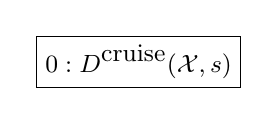
\begin{tikzpicture}
\small
\matrix[nodes={minimum size=6mm}] {
  \node[draw] {$0:D^\textrm{cruise}(\mathcal{X},s)$};\\
};
\end{tikzpicture}

where $s$ is the server identified by {\tt{}sid} (param. 1).\\
\textbf{Side Effects:} none.\\
\textbf{Throws:} {\tt{}SQLException} if database failure is encountered.\\
\bottomrule
\end{tabular}
\nwenddocs{}\nwbegincode{239}\sublabel{NW27XAxz-1Ang64-8}\nwmargintag{{\nwtagstyle{}\subpageref{NW27XAxz-1Ang64-8}}}\moddef{Query various metrics~{\nwtagstyle{}\subpageref{NW27XAxz-1Ang64-1}}}\plusendmoddef
public int[] DBQueryServerCruisingDistance(final int sid) throws SQLException \{
  try (\LA{}Open \code{}conn\edoc{}~{\nwtagstyle{}\subpageref{NW27XAxz-JT1v9-1}}\RA{}) \{
    return DBFetch(conn, "S106", 1, sid);
  \} catch (SQLException e) \{
    throw e;
  \}
\}
\nwindexdefn{DBQueryServerCruisingDistance}{DBQueryServerCruisingDistance}{NW27XAxz-1Ang64-8}\eatline
\nwidentdefs{\\{{DBQueryServerCruisingDistance}{DBQueryServerCruisingDistance}}}\nwidentuses{\\{{DBFetch}{DBFetch}}\\{{S106}{S106}}}\nwindexuse{DBFetch}{DBFetch}{NW27XAxz-1Ang64-8}\nwindexuse{S106}{S106}{NW27XAxz-1Ang64-8}\nwendcode{}\nwbegindocs{240}\nwdocspar
\subsection{{\tt{}\protect\nwindexuse{DBQueryServerCruisingDistanceTotal}{DBQueryServerCruisingDistanceTotal}{NW27XAxz-1Ang64-9}DBQueryServerCruisingDistanceTotal}(0)}
\begin{tabular}{p{\textwidth}}
\toprule
\rowcolor{TableTitle}
Method \textcolor{blue}{{\tt{}\protect\nwindexuse{DBQueryServerCruisingDistanceTotal}{DBQueryServerCruisingDistanceTotal}{NW27XAxz-1Ang64-9}DBQueryServerCruisingDistanceTotal}}(0) returns the
total cruising distance of all servers.
A {\tt{}SQLException} is thrown in case of database failure.\\
\midrule
\textbf{Parameters:} none.\\
\textbf{Returns:} results of the query flattened into an integer array,
or {\tt{}null} if no results.

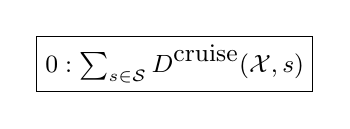
\begin{tikzpicture}
\small
\matrix[nodes={minimum size=6mm}] {
  \node[draw] {$0:\sum_{s\in\mathcal{S}}D^\textrm{cruise}(\mathcal{X},s)$};\\
};
\end{tikzpicture}\\
\textbf{Side Effects:} none.\\
\textbf{Throws:} {\tt{}SQLException} if database failure is encountered.\\
\bottomrule
\end{tabular}
\nwenddocs{}\nwbegincode{241}\sublabel{NW27XAxz-1Ang64-9}\nwmargintag{{\nwtagstyle{}\subpageref{NW27XAxz-1Ang64-9}}}\moddef{Query various metrics~{\nwtagstyle{}\subpageref{NW27XAxz-1Ang64-1}}}\plusendmoddef
public int[] DBQueryServerCruisingDistanceTotal() throws SQLException \{
  try (\LA{}Open \code{}conn\edoc{}~{\nwtagstyle{}\subpageref{NW27XAxz-JT1v9-1}}\RA{}) \{
    return DBFetch(conn, "S107", 1);
  \} catch (SQLException e) \{
    throw e;
  \}
\}
\nwindexdefn{DBQueryServerCruisingDistanceTotal}{DBQueryServerCruisingDistanceTotal}{NW27XAxz-1Ang64-9}\eatline
\nwidentdefs{\\{{DBQueryServerCruisingDistanceTotal}{DBQueryServerCruisingDistanceTotal}}}\nwidentuses{\\{{DBFetch}{DBFetch}}\\{{S107}{S107}}}\nwindexuse{DBFetch}{DBFetch}{NW27XAxz-1Ang64-9}\nwindexuse{S107}{S107}{NW27XAxz-1Ang64-9}\nwendcode{}\nwbegindocs{242}\nwdocspar
\subsection{{\tt{}\protect\nwindexuse{DBQueryServerServiceDistance}{DBQueryServerServiceDistance}{NW27XAxz-1Ang64-A}DBQueryServerServiceDistance}(1)}
\begin{tabular}{p{\textwidth}}
\toprule
\rowcolor{TableTitle}
Method \textcolor{blue}{{\tt{}\protect\nwindexuse{DBQueryServerServiceDistance}{DBQueryServerServiceDistance}{NW27XAxz-1Ang64-A}DBQueryServerServiceDistance}}(1) returns the
service distance $D^\textrm{service}(\mathcal{X},s)$
(Eq.~\ref{eq:service-distance}) of the given server.
A {\tt{}SQLException} is thrown in case of database failure.\\
\midrule
\textbf{Parameters:}\\
\begin{tabular}{lp{116mm}}
Integer {\tt{}sid} (param. 1):&server identifier.
\end{tabular}\\
\textbf{Returns:} results of the query flattened into an integer array,
or {\tt{}null} if no results.

\begin{tikzpicture}
\small
\matrix[nodes={minimum size=6mm}] {
  \node[draw] {$0:D^\textrm{service}(\mathcal{X},s)$};\\
};
\end{tikzpicture}

where $s$ is the server identified by {\tt{}sid} (param. 1).\\
\textbf{Side Effects:} none.\\
\textbf{Throws:} {\tt{}SQLException} if database failure is encountered.\\
\bottomrule
\end{tabular}
\nwenddocs{}\nwbegincode{243}\sublabel{NW27XAxz-1Ang64-A}\nwmargintag{{\nwtagstyle{}\subpageref{NW27XAxz-1Ang64-A}}}\moddef{Query various metrics~{\nwtagstyle{}\subpageref{NW27XAxz-1Ang64-1}}}\plusendmoddef
public int[] DBQueryServerServiceDistance(final int sid) throws SQLException \{
  try (\LA{}Open \code{}conn\edoc{}~{\nwtagstyle{}\subpageref{NW27XAxz-JT1v9-1}}\RA{}) \{
    return DBFetch(conn, "S108", 1, sid);
  \} catch (SQLException e) \{
    throw e;
  \}
\}
\nwindexdefn{DBQueryServerServiceDistance}{DBQueryServerServiceDistance}{NW27XAxz-1Ang64-A}\eatline
\nwidentdefs{\\{{DBQueryServerServiceDistance}{DBQueryServerServiceDistance}}}\nwidentuses{\\{{DBFetch}{DBFetch}}\\{{S108}{S108}}}\nwindexuse{DBFetch}{DBFetch}{NW27XAxz-1Ang64-A}\nwindexuse{S108}{S108}{NW27XAxz-1Ang64-A}\nwendcode{}\nwbegindocs{244}\nwdocspar
\subsection{{\tt{}\protect\nwindexuse{DBQueryServerServiceDistanceTotal}{DBQueryServerServiceDistanceTotal}{NW27XAxz-1Ang64-B}DBQueryServerServiceDistanceTotal}(0)}
\begin{tabular}{p{\textwidth}}
\toprule
\rowcolor{TableTitle}
Method \textcolor{blue}{{\tt{}\protect\nwindexuse{DBQueryServerServiceDistanceTotal}{DBQueryServerServiceDistanceTotal}{NW27XAxz-1Ang64-B}DBQueryServerServiceDistanceTotal}}(0) returns the
total service distance of all servers.
A {\tt{}SQLException} is thrown in case of database failure.\\
\midrule
\textbf{Parameters:} none.\\
\textbf{Returns:} results of the query flattened into an integer array,
or {\tt{}null} if no results.

\begin{tikzpicture}
\small
\matrix[nodes={minimum size=6mm}] {
  \node[draw] {$0:\sum_{s\in\mathcal{S}}D^\textrm{service}(\mathcal{X},s)$};\\
};
\end{tikzpicture}\\
\textbf{Side Effects:} none.\\
\textbf{Throws:} {\tt{}SQLException} if database failure is encountered.\\
\bottomrule
\end{tabular}
\nwenddocs{}\nwbegincode{245}\sublabel{NW27XAxz-1Ang64-B}\nwmargintag{{\nwtagstyle{}\subpageref{NW27XAxz-1Ang64-B}}}\moddef{Query various metrics~{\nwtagstyle{}\subpageref{NW27XAxz-1Ang64-1}}}\plusendmoddef
public int[] DBQueryServerServiceDistanceTotal() throws SQLException \{
  try (\LA{}Open \code{}conn\edoc{}~{\nwtagstyle{}\subpageref{NW27XAxz-JT1v9-1}}\RA{}) \{
    return DBFetch(conn, "S109", 1);
  \} catch (SQLException e) \{
    throw e;
  \}
\}
\nwindexdefn{DBQueryServerServiceDistanceTotal}{DBQueryServerServiceDistanceTotal}{NW27XAxz-1Ang64-B}\eatline
\nwidentdefs{\\{{DBQueryServerServiceDistanceTotal}{DBQueryServerServiceDistanceTotal}}}\nwidentuses{\\{{DBFetch}{DBFetch}}\\{{S109}{S109}}}\nwindexuse{DBFetch}{DBFetch}{NW27XAxz-1Ang64-B}\nwindexuse{S109}{S109}{NW27XAxz-1Ang64-B}\nwendcode{}\nwbegindocs{246}\nwdocspar
\subsection{{\tt{}\protect\nwindexuse{DBQueryRequestDetourDistance}{DBQueryRequestDetourDistance}{NW27XAxz-1Ang64-C}DBQueryRequestDetourDistance}(1)}
\begin{tabular}{p{\textwidth}}
\toprule
\rowcolor{TableTitle}
Method \textcolor{blue}{{\tt{}\protect\nwindexuse{DBQueryRequestDetourDistance}{DBQueryRequestDetourDistance}{NW27XAxz-1Ang64-C}DBQueryRequestDetourDistance}}(1) returns the
detour distance $D^\textrm{detour}(\mathcal{X},r)$
(Eq.~\ref{eq:detour-distance}) of the given request.
A {\tt{}SQLException} is thrown in case of database failure.\\
\midrule
\textbf{Parameters:}\\
\begin{tabular}{lp{116mm}}
Integer {\tt{}rid} (param. 1):&request identifier.
\end{tabular}\\
\textbf{Returns:} results of the query flattened into an integer array,
or {\tt{}null} if no results.

\begin{tikzpicture}
\small
\matrix[nodes={minimum size=6mm}] {
  \node[draw] {$0:D^\textrm{detour}(\mathcal{X},r)$};\\
};
\end{tikzpicture}

where $r$ is the request identified by {\tt{}rid} (param. 1).\\
\textbf{Side Effects:} none.\\
\textbf{Throws:} {\tt{}SQLException} if database failure is encountered.\\
\bottomrule
\end{tabular}
\nwenddocs{}\nwbegincode{247}\sublabel{NW27XAxz-1Ang64-C}\nwmargintag{{\nwtagstyle{}\subpageref{NW27XAxz-1Ang64-C}}}\moddef{Query various metrics~{\nwtagstyle{}\subpageref{NW27XAxz-1Ang64-1}}}\plusendmoddef
public int[] DBQueryRequestDetourDistance(final int rid) throws SQLException \{
  try (\LA{}Open \code{}conn\edoc{}~{\nwtagstyle{}\subpageref{NW27XAxz-JT1v9-1}}\RA{}) \{
    return DBFetch(conn, "S112", 1, rid);
  \} catch (SQLException e) \{
    throw e;
  \}
\}
\nwindexdefn{DBQueryRequestDetourDistance}{DBQueryRequestDetourDistance}{NW27XAxz-1Ang64-C}\eatline
\nwidentdefs{\\{{DBQueryRequestDetourDistance}{DBQueryRequestDetourDistance}}}\nwidentuses{\\{{DBFetch}{DBFetch}}\\{{S112}{S112}}}\nwindexuse{DBFetch}{DBFetch}{NW27XAxz-1Ang64-C}\nwindexuse{S112}{S112}{NW27XAxz-1Ang64-C}\nwendcode{}\nwbegindocs{248}\nwdocspar
\subsection{{\tt{}\protect\nwindexuse{DBQueryRequestDetourDistanceTotal}{DBQueryRequestDetourDistanceTotal}{NW27XAxz-1Ang64-D}DBQueryRequestDetourDistanceTotal}(0)}
\begin{tabular}{p{\textwidth}}
\toprule
\rowcolor{TableTitle}
Method \textcolor{blue}{{\tt{}\protect\nwindexuse{DBQueryRequestDetourDistanceTotal}{DBQueryRequestDetourDistanceTotal}{NW27XAxz-1Ang64-D}DBQueryRequestDetourDistanceTotal}}(0) returns the
total detour distance of all requests.
A {\tt{}SQLException} is thrown in case of database failure.\\
\midrule
\textbf{Parameters:} none.\\
\textbf{Returns:} results of the query flattened into an integer array,
or {\tt{}null} if no results.

\begin{tikzpicture}
\small
\matrix[nodes={minimum size=6mm}] {
  \node[draw] {$0:\sum_{r\in\mathcal{R}}D^\textrm{detour}(\mathcal{X},r)$};\\
};
\end{tikzpicture}\\
\textbf{Side Effects:} none.\\
\textbf{Throws:} {\tt{}SQLException} if database failure is encountered.\\
\bottomrule
\end{tabular}
\nwenddocs{}\nwbegincode{249}\sublabel{NW27XAxz-1Ang64-D}\nwmargintag{{\nwtagstyle{}\subpageref{NW27XAxz-1Ang64-D}}}\moddef{Query various metrics~{\nwtagstyle{}\subpageref{NW27XAxz-1Ang64-1}}}\plusendmoddef
public int[] DBQueryRequestDetourDistanceTotal() throws SQLException \{
  try (\LA{}Open \code{}conn\edoc{}~{\nwtagstyle{}\subpageref{NW27XAxz-JT1v9-1}}\RA{}) \{
    return DBFetch(conn, "S113", 1);
  \} catch (SQLException e) \{
    throw e;
  \}
\}
\nwindexdefn{DBQueryRequestDetourDistanceTotal}{DBQueryRequestDetourDistanceTotal}{NW27XAxz-1Ang64-D}\eatline
\nwidentdefs{\\{{DBQueryRequestDetourDistanceTotal}{DBQueryRequestDetourDistanceTotal}}}\nwidentuses{\\{{DBFetch}{DBFetch}}\\{{S113}{S113}}}\nwindexuse{DBFetch}{DBFetch}{NW27XAxz-1Ang64-D}\nwindexuse{S113}{S113}{NW27XAxz-1Ang64-D}\nwendcode{}\nwbegindocs{250}\nwdocspar
\subsection{{\tt{}\protect\nwindexuse{DBQueryRequestTransitDistance}{DBQueryRequestTransitDistance}{NW27XAxz-1Ang64-E}DBQueryRequestTransitDistance}(1)}
\begin{tabular}{p{\textwidth}}
\toprule
\rowcolor{TableTitle}
Method \textcolor{blue}{{\tt{}\protect\nwindexuse{DBQueryRequestTransitDistance}{DBQueryRequestTransitDistance}{NW27XAxz-1Ang64-E}DBQueryRequestTransitDistance}}(1) returns the
transit distance $D^\textrm{transit}(\mathcal{X},r)$
(Eq.~\ref{eq:transit-distance}) of the given request.
A {\tt{}SQLException} is thrown in case of database failure.\\
\midrule
\textbf{Parameters:}\\
\begin{tabular}{lp{116mm}}
Integer {\tt{}rid} (param. 1):&request identifier.
\end{tabular}\\
\textbf{Returns:} results of the query flattened into an integer array,
or {\tt{}null} if no results.

\begin{tikzpicture}
\small
\matrix[nodes={minimum size=6mm}] {
  \node[draw] {$0:D^\textrm{transit}(\mathcal{X},r)$};\\
};
\end{tikzpicture}

where $r$ is the request identified by {\tt{}rid} (param. 1).\\
\textbf{Side Effects:} none.\\
\textbf{Throws:} {\tt{}SQLException} if database failure is encountered.\\
\bottomrule
\end{tabular}
\nwenddocs{}\nwbegincode{251}\sublabel{NW27XAxz-1Ang64-E}\nwmargintag{{\nwtagstyle{}\subpageref{NW27XAxz-1Ang64-E}}}\moddef{Query various metrics~{\nwtagstyle{}\subpageref{NW27XAxz-1Ang64-1}}}\plusendmoddef
public int[] DBQueryRequestTransitDistance(final int rid) throws SQLException \{
  try (\LA{}Open \code{}conn\edoc{}~{\nwtagstyle{}\subpageref{NW27XAxz-JT1v9-1}}\RA{}) \{
    return DBFetch(conn, "S114", 1, rid);
  \} catch (SQLException e) \{
    throw e;
  \}
\}
\nwindexdefn{DBQueryRequestTransitDistance}{DBQueryRequestTransitDistance}{NW27XAxz-1Ang64-E}\eatline
\nwidentdefs{\\{{DBQueryRequestTransitDistance}{DBQueryRequestTransitDistance}}}\nwidentuses{\\{{DBFetch}{DBFetch}}\\{{S114}{S114}}}\nwindexuse{DBFetch}{DBFetch}{NW27XAxz-1Ang64-E}\nwindexuse{S114}{S114}{NW27XAxz-1Ang64-E}\nwendcode{}\nwbegindocs{252}\nwdocspar
\subsection{{\tt{}\protect\nwindexuse{DBQueryRequestTransitDistanceTotal}{DBQueryRequestTransitDistanceTotal}{NW27XAxz-1Ang64-F}DBQueryRequestTransitDistanceTotal}(0)}
\begin{tabular}{p{\textwidth}}
\toprule
\rowcolor{TableTitle}
Method \textcolor{blue}{{\tt{}\protect\nwindexuse{DBQueryRequestTransitDistanceTotal}{DBQueryRequestTransitDistanceTotal}{NW27XAxz-1Ang64-F}DBQueryRequestTransitDistanceTotal}}(0) returns the
total transit distance of all requests.
A {\tt{}SQLException} is thrown in case of database failure.\\
\midrule
\textbf{Parameters:} none.\\
\textbf{Returns:} results of the query flattened into an integer array,
or {\tt{}null} if no results.

\begin{tikzpicture}
\small
\matrix[nodes={minimum size=6mm}] {
  \node[draw] {$0:\sum_{r\in\mathcal{R}}D^\textrm{transit}(\mathcal{X},r)$};\\
};
\end{tikzpicture}\\
\textbf{Side Effects:} none.\\
\textbf{Throws:} {\tt{}SQLException} if database failure is encountered.\\
\bottomrule
\end{tabular}
\nwenddocs{}\nwbegincode{253}\sublabel{NW27XAxz-1Ang64-F}\nwmargintag{{\nwtagstyle{}\subpageref{NW27XAxz-1Ang64-F}}}\moddef{Query various metrics~{\nwtagstyle{}\subpageref{NW27XAxz-1Ang64-1}}}\plusendmoddef
public int[] DBQueryRequestTransitDistanceTotal() throws SQLException \{
  try (\LA{}Open \code{}conn\edoc{}~{\nwtagstyle{}\subpageref{NW27XAxz-JT1v9-1}}\RA{}) \{
    return DBFetch(conn, "S115", 1);
  \} catch (SQLException e) \{
    throw e;
  \}
\}
\nwindexdefn{DBQueryRequestTransitDistanceTotal}{DBQueryRequestTransitDistanceTotal}{NW27XAxz-1Ang64-F}\eatline
\nwidentdefs{\\{{DBQueryRequestTransitDistanceTotal}{DBQueryRequestTransitDistanceTotal}}}\nwidentuses{\\{{DBFetch}{DBFetch}}\\{{S115}{S115}}}\nwindexuse{DBFetch}{DBFetch}{NW27XAxz-1Ang64-F}\nwindexuse{S115}{S115}{NW27XAxz-1Ang64-F}\nwendcode{}\nwbegindocs{254}\nwdocspar
\subsection{{\tt{}\protect\nwindexuse{DBQueryServerTravelDuration}{DBQueryServerTravelDuration}{NW27XAxz-1Ang64-G}DBQueryServerTravelDuration}(1)}
\begin{tabular}{p{\textwidth}}
\toprule
\rowcolor{TableTitle}
Method \textcolor{blue}{{\tt{}\protect\nwindexuse{DBQueryServerTravelDuration}{DBQueryServerTravelDuration}{NW27XAxz-1Ang64-G}DBQueryServerTravelDuration}}(1) returns the
travel duration $\delta^\textrm{travel}(\mathcal{X},r)$
(Eq.~\ref{eq:travel-duration}) of the given server.
A {\tt{}SQLException} is thrown in case of database failure.\\
\midrule
\textbf{Parameters:}\\
\begin{tabular}{lp{116mm}}
Integer {\tt{}sid} (param. 1):&server identifier.
\end{tabular}\\
\textbf{Returns:} results of the query flattened into an integer array,
or {\tt{}null} if no results.

\begin{tikzpicture}
\small
\matrix[nodes={minimum size=6mm}] {
  \node[draw] {$0:\delta^\textrm{travel}(\mathcal{X},s)$};\\
};
\end{tikzpicture}

where $s$ is the server identified by {\tt{}sid} (param. 1).\\
\textbf{Side Effects:} none.\\
\textbf{Throws:} {\tt{}SQLException} if database failure is encountered.\\
\bottomrule
\end{tabular}
\nwenddocs{}\nwbegincode{255}\sublabel{NW27XAxz-1Ang64-G}\nwmargintag{{\nwtagstyle{}\subpageref{NW27XAxz-1Ang64-G}}}\moddef{Query various metrics~{\nwtagstyle{}\subpageref{NW27XAxz-1Ang64-1}}}\plusendmoddef
public int[] DBQueryServerTravelDuration(final int sid) throws SQLException \{
  try (\LA{}Open \code{}conn\edoc{}~{\nwtagstyle{}\subpageref{NW27XAxz-JT1v9-1}}\RA{}) \{
    return DBFetch(conn, "S116", 1, sid);
  \} catch (SQLException e) \{
    throw e;
  \}
\}
\nwindexdefn{DBQueryServerTravelDuration}{DBQueryServerTravelDuration}{NW27XAxz-1Ang64-G}\eatline
\nwidentdefs{\\{{DBQueryServerTravelDuration}{DBQueryServerTravelDuration}}}\nwidentuses{\\{{DBFetch}{DBFetch}}\\{{S116}{S116}}}\nwindexuse{DBFetch}{DBFetch}{NW27XAxz-1Ang64-G}\nwindexuse{S116}{S116}{NW27XAxz-1Ang64-G}\nwendcode{}\nwbegindocs{256}\nwdocspar
\subsection{{\tt{}\protect\nwindexuse{DBQueryServerTravelDurationTotal}{DBQueryServerTravelDurationTotal}{NW27XAxz-1Ang64-H}DBQueryServerTravelDurationTotal}(0)}
\begin{tabular}{p{\textwidth}}
\toprule
\rowcolor{TableTitle}
Method \textcolor{blue}{{\tt{}\protect\nwindexuse{DBQueryServerTravelDurationTotal}{DBQueryServerTravelDurationTotal}{NW27XAxz-1Ang64-H}DBQueryServerTravelDurationTotal}}(0) returns the
total travel duration of all servers.
A {\tt{}SQLException} is thrown in case of database failure.\\
\midrule
\textbf{Parameters:} none.\\
\textbf{Returns:} results of the query flattened into an integer array,
or {\tt{}null} if no results.

\begin{tikzpicture}
\small
\matrix[nodes={minimum size=6mm}] {
  \node[draw] {$0:\sum_{s\in\mathcal{S}}\delta^\textrm{travel}(\mathcal{X},s)$};\\
};
\end{tikzpicture}\\
\textbf{Side Effects:} none.\\
\textbf{Throws:} {\tt{}SQLException} if database failure is encountered.\\
\bottomrule
\end{tabular}
\nwenddocs{}\nwbegincode{257}\sublabel{NW27XAxz-1Ang64-H}\nwmargintag{{\nwtagstyle{}\subpageref{NW27XAxz-1Ang64-H}}}\moddef{Query various metrics~{\nwtagstyle{}\subpageref{NW27XAxz-1Ang64-1}}}\plusendmoddef
public int[] DBQueryServerTravelDurationTotal() throws SQLException \{
  try (\LA{}Open \code{}conn\edoc{}~{\nwtagstyle{}\subpageref{NW27XAxz-JT1v9-1}}\RA{}) \{
    return DBFetch(conn, "S117", 1);
  \} catch (SQLException e) \{
    throw e;
  \}
\}
\nwindexdefn{DBQueryServerTravelDurationTotal}{DBQueryServerTravelDurationTotal}{NW27XAxz-1Ang64-H}\eatline
\nwidentdefs{\\{{DBQueryServerTravelDurationTotal}{DBQueryServerTravelDurationTotal}}}\nwidentuses{\\{{DBFetch}{DBFetch}}\\{{S117}{S117}}}\nwindexuse{DBFetch}{DBFetch}{NW27XAxz-1Ang64-H}\nwindexuse{S117}{S117}{NW27XAxz-1Ang64-H}\nwendcode{}\nwbegindocs{258}\nwdocspar
\subsection{{\tt{}\protect\nwindexuse{DBQueryRequestPickupDuration}{DBQueryRequestPickupDuration}{NW27XAxz-1Ang64-I}DBQueryRequestPickupDuration}(1)}
\begin{tabular}{p{\textwidth}}
\toprule
\rowcolor{TableTitle}
Method \textcolor{blue}{{\tt{}\protect\nwindexuse{DBQueryRequestPickupDuration}{DBQueryRequestPickupDuration}{NW27XAxz-1Ang64-I}DBQueryRequestPickupDuration}}(1) returns the
pickup delay $\delta^\textrm{pickup}(\mathcal{X},r)$
(Eq.~\ref{eq:pick-up delay}) of the given request.
A {\tt{}SQLException} is thrown in case of database failure.\\
\midrule
\textbf{Parameters:}\\
\begin{tabular}{lp{116mm}}
Integer {\tt{}rid} (param. 1):&request identifier.
\end{tabular}\\
\textbf{Returns:} results of the query flattened into an integer array,
or {\tt{}null} if no results.

\begin{tikzpicture}
\small
\matrix[nodes={minimum size=6mm}] {
  \node[draw] {$0:\delta^\textrm{pickup}(\mathcal{X},r)$};\\
};
\end{tikzpicture}

where $r$ is the request identified by {\tt{}rid} (param. 1).\\
\textbf{Side Effects:} none.\\
\textbf{Throws:} {\tt{}SQLException} if database failure is encountered.\\
\bottomrule
\end{tabular}
\nwenddocs{}\nwbegincode{259}\sublabel{NW27XAxz-1Ang64-I}\nwmargintag{{\nwtagstyle{}\subpageref{NW27XAxz-1Ang64-I}}}\moddef{Query various metrics~{\nwtagstyle{}\subpageref{NW27XAxz-1Ang64-1}}}\plusendmoddef
public int[] DBQueryRequestPickupDuration(final int rid) throws SQLException \{
  try (\LA{}Open \code{}conn\edoc{}~{\nwtagstyle{}\subpageref{NW27XAxz-JT1v9-1}}\RA{}) \{
    return DBFetch(conn, "S118", 1, rid);
  \} catch (SQLException e) \{
    throw e;
  \}
\}
\nwindexdefn{DBQueryRequestPickupDuration}{DBQueryRequestPickupDuration}{NW27XAxz-1Ang64-I}\eatline
\nwidentdefs{\\{{DBQueryRequestPickupDuration}{DBQueryRequestPickupDuration}}}\nwidentuses{\\{{DBFetch}{DBFetch}}\\{{S118}{S118}}}\nwindexuse{DBFetch}{DBFetch}{NW27XAxz-1Ang64-I}\nwindexuse{S118}{S118}{NW27XAxz-1Ang64-I}\nwendcode{}\nwbegindocs{260}\nwdocspar
\subsection{{\tt{}\protect\nwindexuse{DBQueryRequestPickupDurationTotal}{DBQueryRequestPickupDurationTotal}{NW27XAxz-1Ang64-J}DBQueryRequestPickupDurationTotal}(0)}
\begin{tabular}{p{\textwidth}}
\toprule
\rowcolor{TableTitle}
Method \textcolor{blue}{{\tt{}\protect\nwindexuse{DBQueryRequestPickupDurationTotal}{DBQueryRequestPickupDurationTotal}{NW27XAxz-1Ang64-J}DBQueryRequestPickupDurationTotal}}(0) returns the
total pickup delay of all requests.
A {\tt{}SQLException} is thrown in case of database failure.\\
\midrule
\textbf{Parameters:} none.\\
\textbf{Returns:} results of the query flattened into an integer array,
or {\tt{}null} if no results.

\begin{tikzpicture}
\small
\matrix[nodes={minimum size=6mm}] {
  \node[draw] {$0:\sum_{r\in\mathcal{R}}\delta^\textrm{pickup}(\mathcal{X},r)$};\\
};
\end{tikzpicture}\\
\textbf{Side Effects:} none.\\
\textbf{Throws:} {\tt{}SQLException} if database failure is encountered.\\
\bottomrule
\end{tabular}
\nwenddocs{}\nwbegincode{261}\sublabel{NW27XAxz-1Ang64-J}\nwmargintag{{\nwtagstyle{}\subpageref{NW27XAxz-1Ang64-J}}}\moddef{Query various metrics~{\nwtagstyle{}\subpageref{NW27XAxz-1Ang64-1}}}\plusendmoddef
public int[] DBQueryRequestPickupDurationTotal() throws SQLException \{
  try (\LA{}Open \code{}conn\edoc{}~{\nwtagstyle{}\subpageref{NW27XAxz-JT1v9-1}}\RA{}) \{
    return DBFetch(conn, "S119", 1);
  \} catch (SQLException e) \{
    throw e;
  \}
\}
\nwindexdefn{DBQueryRequestPickupDurationTotal}{DBQueryRequestPickupDurationTotal}{NW27XAxz-1Ang64-J}\eatline
\nwidentdefs{\\{{DBQueryRequestPickupDurationTotal}{DBQueryRequestPickupDurationTotal}}}\nwidentuses{\\{{DBFetch}{DBFetch}}\\{{S119}{S119}}}\nwindexuse{DBFetch}{DBFetch}{NW27XAxz-1Ang64-J}\nwindexuse{S119}{S119}{NW27XAxz-1Ang64-J}\nwendcode{}\nwbegindocs{262}\nwdocspar
\subsection{{\tt{}\protect\nwindexuse{DBQueryRequestTransitDuration}{DBQueryRequestTransitDuration}{NW27XAxz-1Ang64-K}DBQueryRequestTransitDuration}(1)}
\begin{tabular}{p{\textwidth}}
\toprule
\rowcolor{TableTitle}
Method \textcolor{blue}{{\tt{}\protect\nwindexuse{DBQueryRequestTransitDuration}{DBQueryRequestTransitDuration}{NW27XAxz-1Ang64-K}DBQueryRequestTransitDuration}}(1) returns the
transit duration $\delta^\textrm{transit}(\mathcal{X},r)$
(Eq.~\ref{eq:transit-duration}) of the given request.
A {\tt{}SQLException} is thrown in case of database failure.\\
\midrule
\textbf{Parameters:}\\
\begin{tabular}{lp{116mm}}
Integer {\tt{}rid} (param. 1):&request identifier.
\end{tabular}\\
\textbf{Returns:} results of the query flattened into an integer array,
or {\tt{}null} if no results.

\begin{tikzpicture}
\small
\matrix[nodes={minimum size=6mm}] {
  \node[draw] {$0:\delta^\textrm{transit}(\mathcal{X},r)$};\\
};
\end{tikzpicture}

where $r$ is the request identified by {\tt{}rid} (param. 1).\\
\textbf{Side Effects:} none.\\
\textbf{Throws:} {\tt{}SQLException} if database failure is encountered.\\
\bottomrule
\end{tabular}
\nwenddocs{}\nwbegincode{263}\sublabel{NW27XAxz-1Ang64-K}\nwmargintag{{\nwtagstyle{}\subpageref{NW27XAxz-1Ang64-K}}}\moddef{Query various metrics~{\nwtagstyle{}\subpageref{NW27XAxz-1Ang64-1}}}\plusendmoddef
public int[] DBQueryRequestTransitDuration(final int rid) throws SQLException \{
  try (\LA{}Open \code{}conn\edoc{}~{\nwtagstyle{}\subpageref{NW27XAxz-JT1v9-1}}\RA{}) \{
    return DBFetch(conn, "S120", 1, rid);
  \} catch (SQLException e) \{
    throw e;
  \}
\}
\nwindexdefn{DBQueryRequestTransitDuration}{DBQueryRequestTransitDuration}{NW27XAxz-1Ang64-K}\eatline
\nwidentdefs{\\{{DBQueryRequestTransitDuration}{DBQueryRequestTransitDuration}}}\nwidentuses{\\{{DBFetch}{DBFetch}}\\{{S120}{S120}}}\nwindexuse{DBFetch}{DBFetch}{NW27XAxz-1Ang64-K}\nwindexuse{S120}{S120}{NW27XAxz-1Ang64-K}\nwendcode{}\nwbegindocs{264}\nwdocspar
\subsection{{\tt{}\protect\nwindexuse{DBQueryRequestTransitDurationTotal}{DBQueryRequestTransitDurationTotal}{NW27XAxz-1Ang64-L}DBQueryRequestTransitDurationTotal}(0)}
\begin{tabular}{p{\textwidth}}
\toprule
\rowcolor{TableTitle}
Method \textcolor{blue}{{\tt{}\protect\nwindexuse{DBQueryRequestTransitDurationTotal}{DBQueryRequestTransitDurationTotal}{NW27XAxz-1Ang64-L}DBQueryRequestTransitDurationTotal}}(0) returns the
total transit duration of all requests.
A {\tt{}SQLException} is thrown in case of database failure.\\
\midrule
\textbf{Parameters:} none.\\
\textbf{Returns:} results of the query flattened into an integer array,
or {\tt{}null} if no results.

\begin{tikzpicture}
\small
\matrix[nodes={minimum size=6mm}] {
  \node[draw] {$0:\sum_{r\in\mathcal{R}}\delta^\textrm{transit}(\mathcal{X},r)$};\\
};
\end{tikzpicture}\\
\textbf{Side Effects:} none.\\
\textbf{Throws:} {\tt{}SQLException} if database failure is encountered.\\
\bottomrule
\end{tabular}
\nwenddocs{}\nwbegincode{265}\sublabel{NW27XAxz-1Ang64-L}\nwmargintag{{\nwtagstyle{}\subpageref{NW27XAxz-1Ang64-L}}}\moddef{Query various metrics~{\nwtagstyle{}\subpageref{NW27XAxz-1Ang64-1}}}\plusendmoddef
public int[] DBQueryRequestTransitDurationTotal() throws SQLException \{
  try (\LA{}Open \code{}conn\edoc{}~{\nwtagstyle{}\subpageref{NW27XAxz-JT1v9-1}}\RA{}) \{
    return DBFetch(conn, "S121", 1);
  \} catch (SQLException e) \{
    throw e;
  \}
\}
\nwindexdefn{DBQueryRequestTransitDurationTotal}{DBQueryRequestTransitDurationTotal}{NW27XAxz-1Ang64-L}\eatline
\nwidentdefs{\\{{DBQueryRequestTransitDurationTotal}{DBQueryRequestTransitDurationTotal}}}\nwidentuses{\\{{DBFetch}{DBFetch}}\\{{S121}{S121}}}\nwindexuse{DBFetch}{DBFetch}{NW27XAxz-1Ang64-L}\nwindexuse{S121}{S121}{NW27XAxz-1Ang64-L}\nwendcode{}\nwbegindocs{266}\nwdocspar
\subsection{{\tt{}\protect\nwindexuse{DBQueryRequestTravelDuration}{DBQueryRequestTravelDuration}{NW27XAxz-1Ang64-M}DBQueryRequestTravelDuration}(1)}
\begin{tabular}{p{\textwidth}}
\toprule
\rowcolor{TableTitle}
Method \textcolor{blue}{{\tt{}\protect\nwindexuse{DBQueryRequestTravelDuration}{DBQueryRequestTravelDuration}{NW27XAxz-1Ang64-M}DBQueryRequestTravelDuration}}(1) returns the
travel duration $\delta^\textrm{travel}(\mathcal{X},r)$
(Eq.~\ref{eq:travel-duration}) of the given request.
A {\tt{}SQLException} is thrown in case of database failure.\\
\midrule
\textbf{Parameters:}\\
\begin{tabular}{lp{116mm}}
Integer {\tt{}rid} (param. 1):&request identifier.
\end{tabular}\\
\textbf{Returns:} results of the query flattened into an integer array,
or {\tt{}null} if no results.

\begin{tikzpicture}
\small
\matrix[nodes={minimum size=6mm}] {
  \node[draw] {$0:\delta^\textrm{travel}(\mathcal{X},r)$};\\
};
\end{tikzpicture}

where $r$ is the request identified by {\tt{}rid} (param. 1).\\
\textbf{Side Effects:} none.\\
\textbf{Throws:} {\tt{}SQLException} if database failure is encountered.\\
\bottomrule
\end{tabular}
\nwenddocs{}\nwbegincode{267}\sublabel{NW27XAxz-1Ang64-M}\nwmargintag{{\nwtagstyle{}\subpageref{NW27XAxz-1Ang64-M}}}\moddef{Query various metrics~{\nwtagstyle{}\subpageref{NW27XAxz-1Ang64-1}}}\plusendmoddef
public int[] DBQueryRequestTravelDuration(final int rid) throws SQLException \{
  try (\LA{}Open \code{}conn\edoc{}~{\nwtagstyle{}\subpageref{NW27XAxz-JT1v9-1}}\RA{}) \{
    return DBFetch(conn, "S122", 1, rid);
  \} catch (SQLException e) \{
    throw e;
  \}
\}
\nwindexdefn{DBQueryRequestTravelDuration}{DBQueryRequestTravelDuration}{NW27XAxz-1Ang64-M}\eatline
\nwidentdefs{\\{{DBQueryRequestTravelDuration}{DBQueryRequestTravelDuration}}}\nwidentuses{\\{{DBFetch}{DBFetch}}\\{{S122}{S122}}}\nwindexuse{DBFetch}{DBFetch}{NW27XAxz-1Ang64-M}\nwindexuse{S122}{S122}{NW27XAxz-1Ang64-M}\nwendcode{}\nwbegindocs{268}\nwdocspar
\subsection{{\tt{}\protect\nwindexuse{DBQueryRequestTravelDurationTotal}{DBQueryRequestTravelDurationTotal}{NW27XAxz-1Ang64-N}DBQueryRequestTravelDurationTotal}(0)}
\begin{tabular}{p{\textwidth}}
\toprule
\rowcolor{TableTitle}
Method \textcolor{blue}{{\tt{}\protect\nwindexuse{DBQueryRequestTravelDurationTotal}{DBQueryRequestTravelDurationTotal}{NW27XAxz-1Ang64-N}DBQueryRequestTravelDurationTotal}}(0) returns the
total travel duration of all requests.
A {\tt{}SQLException} is thrown in case of database failure.\\
\midrule
\textbf{Parameters:} none.\\
\textbf{Returns:} results of the query flattened into an integer array,
or {\tt{}null} if no results.

\begin{tikzpicture}
\small
\matrix[nodes={minimum size=6mm}] {
  \node[draw] {$0:\sum_{r\in\mathcal{R}}\delta^\textrm{travel}(\mathcal{X},r)$};\\
};
\end{tikzpicture}\\
\textbf{Side Effects:} none.\\
\textbf{Throws:} {\tt{}SQLException} if database failure is encountered.\\
\bottomrule
\end{tabular}
\nwenddocs{}\nwbegincode{269}\sublabel{NW27XAxz-1Ang64-N}\nwmargintag{{\nwtagstyle{}\subpageref{NW27XAxz-1Ang64-N}}}\moddef{Query various metrics~{\nwtagstyle{}\subpageref{NW27XAxz-1Ang64-1}}}\plusendmoddef
public int[] DBQueryRequestTravelDurationTotal() throws SQLException \{
  try (\LA{}Open \code{}conn\edoc{}~{\nwtagstyle{}\subpageref{NW27XAxz-JT1v9-1}}\RA{}) \{
    return DBFetch(conn, "S123", 1);
  \} catch (SQLException e) \{
    throw e;
  \}
\}
\nwindexdefn{DBQueryRequestTravelDurationTotal}{DBQueryRequestTravelDurationTotal}{NW27XAxz-1Ang64-N}\eatline
\nwidentdefs{\\{{DBQueryRequestTravelDurationTotal}{DBQueryRequestTravelDurationTotal}}}\nwidentuses{\\{{DBFetch}{DBFetch}}\\{{S123}{S123}}}\nwindexuse{DBFetch}{DBFetch}{NW27XAxz-1Ang64-N}\nwindexuse{S123}{S123}{NW27XAxz-1Ang64-N}\nwendcode{}\nwbegindocs{270}\nwdocspar
\subsection{{\tt{}\protect\nwindexuse{DBQueryRequestDepartureTime}{DBQueryRequestDepartureTime}{NW27XAxz-1Ang64-O}DBQueryRequestDepartureTime}(1)}
\begin{tabular}{p{\textwidth}}
\toprule
\rowcolor{TableTitle}
Method \textcolor{blue}{{\tt{}\protect\nwindexuse{DBQueryRequestDepartureTime}{DBQueryRequestDepartureTime}{NW27XAxz-1Ang64-O}DBQueryRequestDepartureTime}}(1) returns the
departure time $t^\textrm{depart}(\mathcal{X},r)$
(Eq.~\ref{eq:departure-time}) of the given request.
A {\tt{}SQLException} is thrown in case of database failure.\\
\midrule
\textbf{Parameters:}\\
\begin{tabular}{lp{116mm}}
Integer {\tt{}rid} (param. 1):&request identifier.
\end{tabular}\\
\textbf{Returns:} results of the query flattened into an integer array,
or {\tt{}null} if no results.

\begin{tikzpicture}
\small
\matrix[nodes={minimum size=6mm}] {
  \node[draw] {$0:t^\textrm{depart}(\mathcal{X},r)$};\\
};
\end{tikzpicture}

where $r$ is the request identified by {\tt{}rid} (param. 1).\\
\textbf{Side Effects:} none.\\
\textbf{Throws:} {\tt{}SQLException} if database failure is encountered.\\
\bottomrule
\end{tabular}
\nwenddocs{}\nwbegincode{271}\sublabel{NW27XAxz-1Ang64-O}\nwmargintag{{\nwtagstyle{}\subpageref{NW27XAxz-1Ang64-O}}}\moddef{Query various metrics~{\nwtagstyle{}\subpageref{NW27XAxz-1Ang64-1}}}\plusendmoddef
public int[] DBQueryRequestDepartureTime(final int rid) throws SQLException \{
  try (\LA{}Open \code{}conn\edoc{}~{\nwtagstyle{}\subpageref{NW27XAxz-JT1v9-1}}\RA{}) \{
    return DBFetch(conn, "S124", 1, rid);
  \} catch (SQLException e) \{
    throw e;
  \}
\}
\nwindexdefn{DBQueryRequestDepartureTime}{DBQueryRequestDepartureTime}{NW27XAxz-1Ang64-O}\eatline
\nwidentdefs{\\{{DBQueryRequestDepartureTime}{DBQueryRequestDepartureTime}}}\nwidentuses{\\{{DBFetch}{DBFetch}}\\{{S124}{S124}}}\nwindexuse{DBFetch}{DBFetch}{NW27XAxz-1Ang64-O}\nwindexuse{S124}{S124}{NW27XAxz-1Ang64-O}\nwendcode{}\nwbegindocs{272}\nwdocspar
\subsection{{\tt{}\protect\nwindexuse{DBQueryServerDepartureTime}{DBQueryServerDepartureTime}{NW27XAxz-1Ang64-P}DBQueryServerDepartureTime}(1)}
\begin{tabular}{p{\textwidth}}
\toprule
\rowcolor{TableTitle}
Method \textcolor{blue}{{\tt{}\protect\nwindexuse{DBQueryServerDepartureTime}{DBQueryServerDepartureTime}{NW27XAxz-1Ang64-P}DBQueryServerDepartureTime}}(1) returns the
departure time $t^\textrm{depart}(\mathcal{X},s)$
(Eq.~\ref{eq:departure-time}) of the given server.
A {\tt{}SQLException} is thrown in case of database failure.\\
\midrule
\textbf{Parameters:}\\
\begin{tabular}{lp{116mm}}
Integer {\tt{}sid} (param. 1):&server identifier.
\end{tabular}\\
\textbf{Returns:} results of the query flattened into an integer array,
or {\tt{}null} if no results.

\begin{tikzpicture}
\small
\matrix[nodes={minimum size=6mm}] {
  \node[draw] {$0:t^\textrm{depart}(\mathcal{X},s)$};\\
};
\end{tikzpicture}

where $s$ is the server identified by {\tt{}sid} (param. 1).\\
\textbf{Side Effects:} none.\\
\textbf{Throws:} {\tt{}SQLException} if database failure is encountered.\\
\bottomrule
\end{tabular}
\nwenddocs{}\nwbegincode{273}\sublabel{NW27XAxz-1Ang64-P}\nwmargintag{{\nwtagstyle{}\subpageref{NW27XAxz-1Ang64-P}}}\moddef{Query various metrics~{\nwtagstyle{}\subpageref{NW27XAxz-1Ang64-1}}}\plusendmoddef
public int[] DBQueryServerDepartureTime(final int sid) throws SQLException \{
  try (\LA{}Open \code{}conn\edoc{}~{\nwtagstyle{}\subpageref{NW27XAxz-JT1v9-1}}\RA{}) \{
    return DBFetch(conn, "S125", 1, sid);
  \} catch (SQLException e) \{
    throw e;
  \}
\}
\nwindexdefn{DBQueryServerDepartureTime}{DBQueryServerDepartureTime}{NW27XAxz-1Ang64-P}\eatline
\nwidentdefs{\\{{DBQueryServerDepartureTime}{DBQueryServerDepartureTime}}}\nwidentuses{\\{{DBFetch}{DBFetch}}\\{{S125}{S125}}}\nwindexuse{DBFetch}{DBFetch}{NW27XAxz-1Ang64-P}\nwindexuse{S125}{S125}{NW27XAxz-1Ang64-P}\nwendcode{}\nwbegindocs{274}\nwdocspar
\subsection{{\tt{}\protect\nwindexuse{DBQueryRequestArrivalTime}{DBQueryRequestArrivalTime}{NW27XAxz-1Ang64-Q}DBQueryRequestArrivalTime}(1)}
\begin{tabular}{p{\textwidth}}
\toprule
\rowcolor{TableTitle}
Method \textcolor{blue}{{\tt{}\protect\nwindexuse{DBQueryRequestArrivalTime}{DBQueryRequestArrivalTime}{NW27XAxz-1Ang64-Q}DBQueryRequestArrivalTime}}(1) returns the
arrival time $t^\textrm{arrive}(\mathcal{X},r)$
(Eq.~\ref{eq:arrival-time}) of the given request.
A {\tt{}SQLException} is thrown in case of database failure.\\
\midrule
\textbf{Parameters:}\\
\begin{tabular}{lp{116mm}}
Integer {\tt{}rid} (param. 1):&request identifier.
\end{tabular}\\
\textbf{Returns:} results of the query flattened into an integer array,
or {\tt{}null} if no results.

\begin{tikzpicture}
\small
\matrix[nodes={minimum size=6mm}] {
  \node[draw] {$0:t^\textrm{arrive}(\mathcal{X},r)$};\\
};
\end{tikzpicture}

where $r$ is the request identified by {\tt{}rid} (param. 1).\\
\textbf{Side Effects:} none.\\
\textbf{Throws:} {\tt{}SQLException} if database failure is encountered.\\
\bottomrule
\end{tabular}
\nwenddocs{}\nwbegincode{275}\sublabel{NW27XAxz-1Ang64-Q}\nwmargintag{{\nwtagstyle{}\subpageref{NW27XAxz-1Ang64-Q}}}\moddef{Query various metrics~{\nwtagstyle{}\subpageref{NW27XAxz-1Ang64-1}}}\plusendmoddef
public int[] DBQueryRequestArrivalTime(final int rid) throws SQLException \{
  try (\LA{}Open \code{}conn\edoc{}~{\nwtagstyle{}\subpageref{NW27XAxz-JT1v9-1}}\RA{}) \{
    return DBFetch(conn, "S126", 1, rid);
  \} catch (SQLException e) \{
    throw e;
  \}
\}
\nwindexdefn{DBQueryRequestArrivalTime}{DBQueryRequestArrivalTime}{NW27XAxz-1Ang64-Q}\eatline
\nwidentdefs{\\{{DBQueryRequestArrivalTime}{DBQueryRequestArrivalTime}}}\nwidentuses{\\{{DBFetch}{DBFetch}}\\{{S126}{S126}}}\nwindexuse{DBFetch}{DBFetch}{NW27XAxz-1Ang64-Q}\nwindexuse{S126}{S126}{NW27XAxz-1Ang64-Q}\nwendcode{}\nwbegindocs{276}\nwdocspar
\subsection{{\tt{}\protect\nwindexuse{DBQueryServerArrivalTime}{DBQueryServerArrivalTime}{NW27XAxz-1Ang64-R}DBQueryServerArrivalTime}(1)}
\begin{tabular}{p{\textwidth}}
\toprule
\rowcolor{TableTitle}
Method \textcolor{blue}{{\tt{}\protect\nwindexuse{DBQueryServerArrivalTime}{DBQueryServerArrivalTime}{NW27XAxz-1Ang64-R}DBQueryServerArrivalTime}}(1) returns the
arrival time $t^\textrm{arrive}(\mathcal{X},s)$
(Eq.~\ref{eq:arrival-time}) of the given server.
A {\tt{}SQLException} is thrown in case of database failure.\\
\midrule
\textbf{Parameters:}\\
\begin{tabular}{lp{116mm}}
Integer {\tt{}sid} (param. 1):&server identifier.
\end{tabular}\\
\textbf{Returns:} results of the query flattened into an integer array,
or {\tt{}null} if no results.

\begin{tikzpicture}
\small
\matrix[nodes={minimum size=6mm}] {
  \node[draw] {$0:t^\textrm{arrive}(\mathcal{X},s)$};\\
};
\end{tikzpicture}

where $s$ is the request identified by {\tt{}sid} (param. 1).\\
\textbf{Side Effects:} none.\\
\textbf{Throws:} {\tt{}SQLException} if database failure is encountered.\\
\bottomrule
\end{tabular}
\nwenddocs{}\nwbegincode{277}\sublabel{NW27XAxz-1Ang64-R}\nwmargintag{{\nwtagstyle{}\subpageref{NW27XAxz-1Ang64-R}}}\moddef{Query various metrics~{\nwtagstyle{}\subpageref{NW27XAxz-1Ang64-1}}}\plusendmoddef
public int[] DBQueryServerArrivalTime(final int sid) throws SQLException \{
  try (\LA{}Open \code{}conn\edoc{}~{\nwtagstyle{}\subpageref{NW27XAxz-JT1v9-1}}\RA{}) \{
    return DBFetch(conn, "S127", 1, sid);
  \} catch (SQLException e) \{
    throw e;
  \}
\}
\nwindexdefn{DBQueryServerArrivalTime}{DBQueryServerArrivalTime}{NW27XAxz-1Ang64-R}\eatline
\nwidentdefs{\\{{DBQueryServerArrivalTime}{DBQueryServerArrivalTime}}}\nwidentuses{\\{{DBFetch}{DBFetch}}\\{{S127}{S127}}}\nwindexuse{DBFetch}{DBFetch}{NW27XAxz-1Ang64-R}\nwindexuse{S127}{S127}{NW27XAxz-1Ang64-R}\nwendcode{}\nwbegindocs{278}\nwdocspar
\section{Private Methods}
\label{sec:private}
\nwenddocs{}\nwbegincode{279}\sublabel{NW27XAxz-XGFF1-1}\nwmargintag{{\nwtagstyle{}\subpageref{NW27XAxz-XGFF1-1}}}\moddef{\code{}Storage\edoc{} private methods~{\nwtagstyle{}\subpageref{NW27XAxz-XGFF1-1}}}\endmoddef\nwused{\\{NW27XAxz-3TAldU-1}}
\LA{}Setup JDBC driver~{\nwtagstyle{}\subpageref{NW27XAxz-33Wt2A-1}}\RA{}
\LA{}Initialize statements~{\nwtagstyle{}\subpageref{NW27XAxz-1g2xnv-1}}\RA{}
\LA{}Prepare a prepared statement~{\nwtagstyle{}\subpageref{NW27XAxz-4UQpM2-1}}\RA{}
\LA{}Fetch items from database~{\nwtagstyle{}\subpageref{NW27XAxz-17Zt8W-1}}\RA{}
\LA{}Fill prepared statement~{\nwtagstyle{}\subpageref{NW27XAxz-1ZE0ye-1}}\RA{}
\LA{}Submit prepared statement batch~{\nwtagstyle{}\subpageref{NW27XAxz-322zJf-1}}\RA{}
\nwendcode{}\nwbegindocs{280}\nwdocspar

\subsection{{\tt{}\protect\nosublabel{NW27XAxz-XGFF1-1-u6}\protect\nwindexuse{setupDriver}{setupDriver}{NW27XAxz-33Wt2A-1}setupDriver}(0)}
\begin{tabular}{p{\textwidth}}
\toprule
\rowcolor{TableTitle}
Method \textcolor{blue}{{\tt{}\protect\nwindexuse{setupDriver}{setupDriver}{NW27XAxz-33Wt2A-1}setupDriver}}(0) registers a connection pool to the
JDBC driver.
The connection pool allows us to concurrently submit SQL
commands against the database from different threads.
A {\tt{}SQLException} is thrown in case of database failure.
A {\tt{}ClassNotFoundException} is thrown if the DBCP2 {\tt{}PoolingDriver}
cannot be found.
Portions of this code are licensed by the Apache Software Foundation.\\
\midrule
\textbf{Parameters:} none.\\
\textbf{Returns:} nothing.\\
\textbf{Side Effects:} registers a new connection pool to the JDBC driver manager.\\
\textbf{Throws:} {\tt{}SQLException} if database failure is encountered, or
{\tt{}ClassNotFoundException} if the DBCP2 driver cannot be found.\\
\bottomrule
\end{tabular}
\nwenddocs{}\nwbegincode{281}\sublabel{NW27XAxz-33Wt2A-1}\nwmargintag{{\nwtagstyle{}\subpageref{NW27XAxz-33Wt2A-1}}}\moddef{Setup JDBC driver~{\nwtagstyle{}\subpageref{NW27XAxz-33Wt2A-1}}}\endmoddef\nwused{\\{NW27XAxz-XGFF1-1}}
private void setupDriver() throws SQLException, ClassNotFoundException \{
  connection_factory = new DriverManagerConnectionFactory(CONNECTIONS_URL);
  poolableconnection_factory = new PoolableConnectionFactory(connection_factory, null);
  poolableconnection_factory.setPoolStatements(true);
  poolableconnection_factory.setDefaultAutoCommit(false);
  poolableconnection_factory.setMaxOpenPreparedStatements(STATEMENTS_MAX_COUNT);
  GenericObjectPoolConfig cfg = new GenericObjectPoolConfig();
  cfg.setMinIdle(100000);
  cfg.setMaxIdle(100000);
  cfg.setMaxTotal(100000);
  pool = new GenericObjectPool<>(poolableconnection_factory, cfg);
  poolableconnection_factory.setPool(pool);
  Class.forName("org.apache.commons.dbcp2.PoolingDriver");
  driver = (PoolingDriver) DriverManager.getDriver(CONNECTIONS_DRIVER_URL);
  driver.registerPool(CONNECTIONS_POOL_NAME, pool);
\}
\nwindexdefn{setupDriver}{setupDriver}{NW27XAxz-33Wt2A-1}\eatline
\nwidentdefs{\\{{setupDriver}{setupDriver}}}\nwidentuses{\\{{connection{\char95}factory}{connection:unfactory}}\\{{CONNECTIONS{\char95}DRIVER{\char95}URL}{CONNECTIONS:unDRIVER:unURL}}\\{{CONNECTIONS{\char95}POOL{\char95}NAME}{CONNECTIONS:unPOOL:unNAME}}\\{{CONNECTIONS{\char95}URL}{CONNECTIONS:unURL}}\\{{driver}{driver}}\\{{pool}{pool}}\\{{poolableconnection{\char95}factory}{poolableconnection:unfactory}}\\{{STATEMENTS{\char95}MAX{\char95}COUNT}{STATEMENTS:unMAX:unCOUNT}}}\nwindexuse{connection{\char95}factory}{connection:unfactory}{NW27XAxz-33Wt2A-1}\nwindexuse{CONNECTIONS{\char95}DRIVER{\char95}URL}{CONNECTIONS:unDRIVER:unURL}{NW27XAxz-33Wt2A-1}\nwindexuse{CONNECTIONS{\char95}POOL{\char95}NAME}{CONNECTIONS:unPOOL:unNAME}{NW27XAxz-33Wt2A-1}\nwindexuse{CONNECTIONS{\char95}URL}{CONNECTIONS:unURL}{NW27XAxz-33Wt2A-1}\nwindexuse{driver}{driver}{NW27XAxz-33Wt2A-1}\nwindexuse{pool}{pool}{NW27XAxz-33Wt2A-1}\nwindexuse{poolableconnection{\char95}factory}{poolableconnection:unfactory}{NW27XAxz-33Wt2A-1}\nwindexuse{STATEMENTS{\char95}MAX{\char95}COUNT}{STATEMENTS:unMAX:unCOUNT}{NW27XAxz-33Wt2A-1}\nwendcode{}\nwbegindocs{282}\nwdocspar
\subsection{{\tt{}\protect\nwindexuse{PS}{PS}{NW27XAxz-4UQpM2-1}PS}(2)}
\begin{tabular}{p{\textwidth}}
\toprule
\rowcolor{TableTitle}
Method \textcolor{blue}{{\tt{}\protect\nwindexuse{PS}{PS}{NW27XAxz-4UQpM2-1}PS}}(2) returns a JDBC {\tt{}PreparedStatement} for the
statement string identified by {\tt{}k} (param. 2) on the connection given in
param. 1.  A {\tt{}SQLException} is thrown in case of database failure.\\
\midrule
\textbf{Parameters:} \\
\begin{tabular}{lp{116mm}}
Connection {\tt{}conn} (param. 1):&a JDBC connection.\\
String {\tt{}k} (param. 2):&statement identifier.\\
\end{tabular}\\
\textbf{Returns:} a prepared statement on the connection in param. 1 of the
statement string identified by param. 2.\\
\textbf{Side Effects:} none.\\
\textbf{Throws:} {\tt{}SQLException} if database failure is encountered.\\
\bottomrule
\end{tabular}
\nwenddocs{}\nwbegincode{283}\sublabel{NW27XAxz-4UQpM2-1}\nwmargintag{{\nwtagstyle{}\subpageref{NW27XAxz-4UQpM2-1}}}\moddef{Prepare a prepared statement~{\nwtagstyle{}\subpageref{NW27XAxz-4UQpM2-1}}}\endmoddef\nwused{\\{NW27XAxz-XGFF1-1}}
private PreparedStatement PS(final Connection conn, final String k) throws SQLException \{
  PreparedStatement p = null;
  try \{
    p = conn.prepareStatement(lu_pstr.get(k),
      ResultSet.TYPE_SCROLL_INSENSITIVE, ResultSet.CONCUR_READ_ONLY);
    p.clearBatch();
    p.clearParameters();
  \} catch (SQLException e) \{
    throw e;
  \}
  return p;
\}
\nwindexdefn{PS}{PS}{NW27XAxz-4UQpM2-1}\eatline
\nwidentdefs{\\{{PS}{PS}}}\nwidentuses{\\{{lu{\char95}pstr}{lu:unpstr}}}\nwindexuse{lu{\char95}pstr}{lu:unpstr}{NW27XAxz-4UQpM2-1}\nwendcode{}\nwbegindocs{284}\nwdocspar
\subsection{{\tt{}\protect\nwindexuse{DBFetch}{DBFetch}{NW27XAxz-17Zt8W-1}DBFetch}(3...)}
\begin{tabular}{p{\textwidth}}
\toprule
\rowcolor{TableTitle}
Method \textcolor{blue}{{\tt{}\protect\nwindexuse{DBFetch}{DBFetch}{NW27XAxz-17Zt8W-1}DBFetch}}(3...) executes a predefined {\tt{}SELECT}
query against the Jargo database instance.
A {\tt{}SQLException} is thrown in case of database failure.\\
\midrule
\textbf{Parameters:} \\
\begin{tabular}{lp{116mm}}
Connection {\tt{}conn} (param. 1):&a JDBC connection.\\
String {\tt{}k} (param. 2):&statement identifier.\\
Integer {\tt{}ncols} (param. 3):&number of columns in the selection.\\
Integer... {\tt{}values} (param. 4...):&values to use in the statement, in order
of appearance.
\end{tabular}\\
\textbf{Returns:} results of the query flattened into an integer array,
or {\tt{}null} if no results.

\begin{tikzpicture}
\small
\matrix[nodes={minimum size=6mm}] {
  \node {...};
 &\node[draw] {$in+j:\textrm{value at column $j$, row $i$ of the result set}$};
 &\node {...};\\
};
\end{tikzpicture}

where $i$, $j$ start from 0.\\
\textbf{Side Effects:} none.\\
\textbf{Throws:} {\tt{}SQLException} if database failure is encountered.\\
\bottomrule
\end{tabular}
\nwenddocs{}\nwbegincode{285}\sublabel{NW27XAxz-17Zt8W-1}\nwmargintag{{\nwtagstyle{}\subpageref{NW27XAxz-17Zt8W-1}}}\moddef{Fetch items from database~{\nwtagstyle{}\subpageref{NW27XAxz-17Zt8W-1}}}\endmoddef\nwused{\\{NW27XAxz-XGFF1-1}}
private int[] DBFetch(
    final Connection conn, final String k, final int ncols, final Integer... values)
throws SQLException \{
  int[] output = new int[] \{ \};
  try \{
    PreparedStatement p = PS(conn, k);
    \LA{}..set values for statement~{\nwtagstyle{}\subpageref{NW27XAxz-2m6DFc-1}}\RA{}
    ResultSet res = p.executeQuery();  // <-- if stuck here, investigate locks
    if (res.last() == true) \{
      \LA{}..flatten results~{\nwtagstyle{}\subpageref{NW27XAxz-2Xu6MS-1}}\RA{}
    \}
    res.close();
    p.close();
  \} catch (SQLException e) \{
    throw e;
  \}
  return output;
\}
\nosublabel{NW27XAxz-17Zt8W-1-u2}\nwindexdefn{DBFetch}{DBFetch}{NW27XAxz-17Zt8W-1}\eatline
\nwidentdefs{\\{{DBFetch}{DBFetch}}}\nwidentuses{\\{{PS}{PS}}}\nwindexuse{PS}{PS}{NW27XAxz-17Zt8W-1}\nwendcode{}\nwbegincode{286}\sublabel{NW27XAxz-2m6DFc-1}\nwmargintag{{\nwtagstyle{}\subpageref{NW27XAxz-2m6DFc-1}}}\moddef{..set values for statement~{\nwtagstyle{}\subpageref{NW27XAxz-2m6DFc-1}}}\endmoddef\nwused{\\{NW27XAxz-17Zt8W-1}\\{NW27XAxz-1ZE0ye-1}}
for (int i = 0; i < values.length; i++) \{
  if (values[i] == null) \{
    p.setNull((i + 1), java.sql.Types.INTEGER);
  \} else \{
    p.setInt ((i + 1), values[i]);
  \}
\}
\nwendcode{}\nwbegindocs{287}\nwdocspar

\subsection{{\tt{}\protect\nwindexuse{PSAdd}{PSAdd}{NW27XAxz-1ZE0ye-1}PSAdd}(2...)}
\begin{tabular}{p{\textwidth}}
\toprule
\rowcolor{TableTitle}
Method \textcolor{blue}{{\tt{}\protect\nwindexuse{PSAdd}{PSAdd}{NW27XAxz-1ZE0ye-1}PSAdd}}(2...) adds a prepared statement to
the execution batch.
A {\tt{}SQLException} is thrown in case of database failure.\\
\midrule
\textbf{Parameters:} \\
\begin{tabular}{lp{116mm}}
Prepared statement {\tt{}p} (param. 1):&a prepared statement.\\
Integer... {\tt{}values} (param. 2...):&values to use in the statement, in order of appearance.\\
\end{tabular}\\
\textbf{Returns:} nothing.\\
\textbf{Side Effects:} adds to the execution batch for the statement in param. 1.\\
\textbf{Throws:} {\tt{}SQLException} if database failure is encountered.\\
\bottomrule
\end{tabular}
\nwenddocs{}\nwbegincode{288}\sublabel{NW27XAxz-1ZE0ye-1}\nwmargintag{{\nwtagstyle{}\subpageref{NW27XAxz-1ZE0ye-1}}}\moddef{Fill prepared statement~{\nwtagstyle{}\subpageref{NW27XAxz-1ZE0ye-1}}}\endmoddef\nwused{\\{NW27XAxz-XGFF1-1}}
private void PSAdd(PreparedStatement p, final Integer... values) throws SQLException \{
  p.clearParameters();
  \LA{}..set values for statement~{\nwtagstyle{}\subpageref{NW27XAxz-2m6DFc-1}}\RA{}
  try \{
    p.addBatch();
  \} catch (SQLException e) \{
    throw e;
  \}
\}
\nosublabel{NW27XAxz-1ZE0ye-1-u1}\nwindexdefn{PSAdd}{PSAdd}{NW27XAxz-1ZE0ye-1}\eatline
\nwidentdefs{\\{{PSAdd}{PSAdd}}}\nwendcode{}\nwbegindocs{289}\nwdocspar
\subsection{{\tt{}\protect\nwindexuse{PSSubmit}{PSSubmit}{NW27XAxz-322zJf-1}PSSubmit}(1...)}
\begin{tabular}{p{\textwidth}}
\toprule
\rowcolor{TableTitle}
Method \textcolor{blue}{{\tt{}\protect\nwindexuse{PSSubmit}{PSSubmit}{NW27XAxz-322zJf-1}PSSubmit}}(1...) executes a prepared statement's batch.
A {\tt{}SQLException} is thrown in case of database failure.\\
\midrule
\textbf{Parameters:} \\
\begin{tabular}{lp{116mm}}
Prepared statement {\tt{}p} (param. 1):&a prepared statement.
\end{tabular}\\
\textbf{Returns:} nothing.\\
\textbf{Side Effects:} may modify tables in the Jargo database.
\textbf{Throws:} {\tt{}SQLException} if database failure is encountered.\\
\bottomrule
\end{tabular}
\nwenddocs{}\nwbegincode{290}\sublabel{NW27XAxz-322zJf-1}\nwmargintag{{\nwtagstyle{}\subpageref{NW27XAxz-322zJf-1}}}\moddef{Submit prepared statement batch~{\nwtagstyle{}\subpageref{NW27XAxz-322zJf-1}}}\endmoddef\nwused{\\{NW27XAxz-XGFF1-1}}
private void PSSubmit(PreparedStatement... statements) throws SQLException \{
  try \{
    for (PreparedStatement p : statements) \{
      p.executeBatch();
      p.close();
    \}
  \} catch (SQLException e) \{
    throw e;
  \}
\}
\nwindexdefn{PSSubmit}{PSSubmit}{NW27XAxz-322zJf-1}\eatline
\nwidentdefs{\\{{PSSubmit}{PSSubmit}}}\nwendcode{}\nwbegindocs{291}\nwdocspar
\subsection{{\tt{}\protect\nwindexuse{PSInit}{PSInit}{NW27XAxz-1g2xnv-1}PSInit}(0)}
\begin{tabular}{p{\textwidth}}
\toprule
\rowcolor{TableTitle}
Method \textcolor{blue}{{\tt{}\protect\nwindexuse{PSInit}{PSInit}{NW27XAxz-1g2xnv-1}PSInit}}(0) initializes the statement cache
{\tt{}\protect\nwindexuse{lu{\char95}pstr}{lu:unpstr}{NW27XAxz-17yXws-2}lu{\char95}pstr}. Each statement is placed in its own chunk so it can be referenced
wherever the statement is used.\\
\midrule
\textbf{Parameters:} none.\\
\textbf{Returns:} nothing.\\
\textbf{Side Effects:} populates {\tt{}\protect\nwindexuse{lu{\char95}pstr}{lu:unpstr}{NW27XAxz-17yXws-2}lu{\char95}pstr}.
\textbf{Throws:} nothing.\\
\bottomrule
\end{tabular}
\nwenddocs{}\nwbegincode{292}\sublabel{NW27XAxz-1g2xnv-1}\nwmargintag{{\nwtagstyle{}\subpageref{NW27XAxz-1g2xnv-1}}}\moddef{Initialize statements~{\nwtagstyle{}\subpageref{NW27XAxz-1g2xnv-1}}}\endmoddef\nwused{\\{NW27XAxz-XGFF1-1}}
private void PSInit() \{
  String INS = "INSERT INTO ";
  String UPD = "UPDATE ";
  String DEL = "DELETE FROM ";
  String SEL = "SELECT ";
  String q2  = "(?,?)";
  String q3  = "(?,?,?)";
  String q4  = "(?,?,?,?)";
  String q7  = "(?,?,?,?,?,?,?)";
  String q8  = "(?,?,?,?,?,?,?,?)";
  String q9  = "(?,?,?,?,?,?,?,?,?)";
  String q12 = "(?,?,?,?,?,?,?,?,?,?,?,?)";
  String q14 = "(?,?,?,?,?,?,?,?,?,?,?,?,?,?)";
  \LA{}S0~{\nwtagstyle{}\subpageref{NW27XAxz-9czRY-1}}\RA{}
  \LA{}S1~{\nwtagstyle{}\subpageref{NW27XAxz-4dnsum-1}}\RA{}
  \LA{}S2~{\nwtagstyle{}\subpageref{NW27XAxz-26Y6r2-1}}\RA{}
  \LA{}S3~{\nwtagstyle{}\subpageref{NW27XAxz-2UOPmS-1}}\RA{}
  \LA{}S4~{\nwtagstyle{}\subpageref{NW27XAxz-yRBj6-1}}\RA{}
  \LA{}S5~{\nwtagstyle{}\subpageref{NW27XAxz-3WGA2y-1}}\RA{}
  \LA{}S6~{\nwtagstyle{}\subpageref{NW27XAxz-1SWfVw-1}}\RA{}
  \LA{}S7~{\nwtagstyle{}\subpageref{NW27XAxz-3Q0zBY-1}}\RA{}
  \LA{}S8~{\nwtagstyle{}\subpageref{NW27XAxz-PwvQG-1}}\RA{}
  \LA{}S9~{\nwtagstyle{}\subpageref{NW27XAxz-4Ai05A-1}}\RA{}
  \LA{}S10~{\nwtagstyle{}\subpageref{NW27XAxz-96fbA-1}}\RA{}
  \LA{}S11~{\nwtagstyle{}\subpageref{NW27XAxz-4dHZ4O-1}}\RA{}
  \LA{}S12~{\nwtagstyle{}\subpageref{NW27XAxz-261n0e-1}}\RA{}
  \LA{}S13~{\nwtagstyle{}\subpageref{NW27XAxz-2Ts5w4-1}}\RA{}
  \LA{}S14~{\nwtagstyle{}\subpageref{NW27XAxz-yU48q-1}}\RA{}
  \LA{}S15~{\nwtagstyle{}\subpageref{NW27XAxz-3WJ2Si-1}}\RA{}
  \LA{}S131~{\nwtagstyle{}\subpageref{NW27XAxz-3WHOrj-1}}\RA{}
  \LA{}S77~{\nwtagstyle{}\subpageref{NW27XAxz-3PlVaO-1}}\RA{}
  \LA{}S84~{\nwtagstyle{}\subpageref{NW27XAxz-yx2fc-1}}\RA{}
  \LA{}S82~{\nwtagstyle{}\subpageref{NW27XAxz-25vZHI-1}}\RA{}
  \LA{}S83~{\nwtagstyle{}\subpageref{NW27XAxz-2TlsCi-1}}\RA{}
  \LA{}S76~{\nwtagstyle{}\subpageref{NW27XAxz-1SHBum-1}}\RA{}
  \LA{}S42~{\nwtagstyle{}\subpageref{NW27XAxz-25mK0a-1}}\RA{}
  \LA{}S43~{\nwtagstyle{}\subpageref{NW27XAxz-2Tccw0-1}}\RA{}
  \LA{}S80~{\nwtagstyle{}\subpageref{NW27XAxz-A8qO4-1}}\RA{}
  \LA{}S62~{\nwtagstyle{}\subpageref{NW27XAxz-25gPSO-1}}\RA{}
  \LA{}S64~{\nwtagstyle{}\subpageref{NW27XAxz-zH56q-1}}\RA{}
  \LA{}S63~{\nwtagstyle{}\subpageref{NW27XAxz-2TWiNo-1}}\RA{}
  \LA{}S65~{\nwtagstyle{}\subpageref{NW27XAxz-3X63Qi-1}}\RA{}
  \LA{}S46~{\nwtagstyle{}\subpageref{NW27XAxz-1RksfU-1}}\RA{}
  \LA{}S130~{\nwtagstyle{}\subpageref{NW27XAxz-ySQXr-1}}\RA{}
  \LA{}S70~{\nwtagstyle{}\subpageref{NW27XAxz-9NVqO-1}}\RA{}
  \LA{}S48~{\nwtagstyle{}\subpageref{NW27XAxz-PSjhs-1}}\RA{}
  \LA{}S66~{\nwtagstyle{}\subpageref{NW27XAxz-1SEANQ-1}}\RA{}
  \LA{}S75~{\nwtagstyle{}\subpageref{NW27XAxz-3W0gRo-1}}\RA{}
  \LA{}S51~{\nwtagstyle{}\subpageref{NW27XAxz-4dVWIm-1}}\RA{}
  \LA{}S67~{\nwtagstyle{}\subpageref{NW27XAxz-3PiU32-1}}\RA{}
  \LA{}S59~{\nwtagstyle{}\subpageref{NW27XAxz-4APdTA-1}}\RA{}
  \LA{}S128~{\nwtagstyle{}\subpageref{NW27XAxz-nIIRf-1}}\RA{}
  \LA{}S60~{\nwtagstyle{}\subpageref{NW27XAxz-9tgZA-1}}\RA{}
  \LA{}S129~{\nwtagstyle{}\subpageref{NW27XAxz-44X5Zr-1}}\RA{}
  \LA{}S61~{\nwtagstyle{}\subpageref{NW27XAxz-4e4a2O-1}}\RA{}
  \LA{}S69~{\nwtagstyle{}\subpageref{NW27XAxz-49qIgW-1}}\RA{}
  \LA{}S68~{\nwtagstyle{}\subpageref{NW27XAxz-P5E1c-1}}\RA{}
  \LA{}S85~{\nwtagstyle{}\subpageref{NW27XAxz-3Wm0zU-1}}\RA{}
  \LA{}S86~{\nwtagstyle{}\subpageref{NW27XAxz-1Ru7wC-1}}\RA{}
  \LA{}S73~{\nwtagstyle{}\subpageref{NW27XAxz-2U8wBI-1}}\RA{}
  \LA{}S87~{\nwtagstyle{}\subpageref{NW27XAxz-3PORbo-1}}\RA{}
  \LA{}S100~{\nwtagstyle{}\subpageref{NW27XAxz-yxMXz-1}}\RA{}
  \LA{}S101~{\nwtagstyle{}\subpageref{NW27XAxz-3WmKrr-1}}\RA{}
  \LA{}S102~{\nwtagstyle{}\subpageref{NW27XAxz-1RuRoZ-1}}\RA{}
  \LA{}S103~{\nwtagstyle{}\subpageref{NW27XAxz-3POlUB-1}}\RA{}
  \LA{}S104~{\nwtagstyle{}\subpageref{NW27XAxz-A9AGR-1}}\RA{}
  \LA{}S105~{\nwtagstyle{}\subpageref{NW27XAxz-4eK3jf-1}}\RA{}
  \LA{}S106~{\nwtagstyle{}\subpageref{NW27XAxz-25vt9f-1}}\RA{}
  \LA{}S107~{\nwtagstyle{}\subpageref{NW27XAxz-2TmC55-1}}\RA{}
  \LA{}S108~{\nwtagstyle{}\subpageref{NW27XAxz-mtPWF-1}}\RA{}
  \LA{}S109~{\nwtagstyle{}\subpageref{NW27XAxz-448CeR-1}}\RA{}
  \LA{}S110~{\nwtagstyle{}\subpageref{NW27XAxz-yTwJX-1}}\RA{}
  \LA{}S111~{\nwtagstyle{}\subpageref{NW27XAxz-3WIudP-1}}\RA{}
  \LA{}S112~{\nwtagstyle{}\subpageref{NW27XAxz-1SZQ6N-1}}\RA{}
  \LA{}S113~{\nwtagstyle{}\subpageref{NW27XAxz-3Q3jlz-1}}\RA{}
  \LA{}S114~{\nwtagstyle{}\subpageref{NW27XAxz-96Xlr-1}}\RA{}
  \LA{}S115~{\nwtagstyle{}\subpageref{NW27XAxz-4dHRF5-1}}\RA{}
  \LA{}S116~{\nwtagstyle{}\subpageref{NW27XAxz-261fBL-1}}\RA{}
  \LA{}S117~{\nwtagstyle{}\subpageref{NW27XAxz-2Try6l-1}}\RA{}
  \LA{}S118~{\nwtagstyle{}\subpageref{NW27XAxz-npyw7-1}}\RA{}
  \LA{}S119~{\nwtagstyle{}\subpageref{NW27XAxz-454m4J-1}}\RA{}
  \LA{}S120~{\nwtagstyle{}\subpageref{NW27XAxz-z4eLL-1}}\RA{}
  \LA{}S121~{\nwtagstyle{}\subpageref{NW27XAxz-3WtcfD-1}}\RA{}
  \LA{}S122~{\nwtagstyle{}\subpageref{NW27XAxz-1S1jbv-1}}\RA{}
  \LA{}S123~{\nwtagstyle{}\subpageref{NW27XAxz-3PW3HX-1}}\RA{}
  \LA{}S124~{\nwtagstyle{}\subpageref{NW27XAxz-9hFnf-1}}\RA{}
  \LA{}S125~{\nwtagstyle{}\subpageref{NW27XAxz-4ds9Gt-1}}\RA{}
  \LA{}S126~{\nwtagstyle{}\subpageref{NW27XAxz-25Tygt-1}}\RA{}
  \LA{}S127~{\nwtagstyle{}\subpageref{NW27XAxz-2TKHcJ-1}}\RA{}
  \LA{}S133~{\nwtagstyle{}\subpageref{NW27XAxz-3Q2E0J-1}}\RA{}
  \LA{}S134~{\nwtagstyle{}\subpageref{NW27XAxz-9eEGJ-1}}\RA{}
  \LA{}S135~{\nwtagstyle{}\subpageref{NW27XAxz-4dp7jX-1}}\RA{}
  \LA{}S136~{\nwtagstyle{}\subpageref{NW27XAxz-26ZLfn-1}}\RA{}
  \LA{}S137~{\nwtagstyle{}\subpageref{NW27XAxz-2UPebD-1}}\RA{}
  \LA{}S138~{\nwtagstyle{}\subpageref{NW27XAxz-nWs2N-1}}\RA{}
  \LA{}S139~{\nwtagstyle{}\subpageref{NW27XAxz-44lfAZ-1}}\RA{}
  \LA{}S140~{\nwtagstyle{}\subpageref{NW27XAxz-yno67-1}}\RA{}
  \LA{}S141~{\nwtagstyle{}\subpageref{NW27XAxz-3WcmPz-1}}\RA{}
  \LA{}S142~{\nwtagstyle{}\subpageref{NW27XAxz-1RktMh-1}}\RA{}
  \LA{}S143~{\nwtagstyle{}\subpageref{NW27XAxz-3PFD2J-1}}\RA{}
  \LA{}S144~{\nwtagstyle{}\subpageref{NW27XAxz-9zboZ-1}}\RA{}
  \LA{}S145~{\nwtagstyle{}\subpageref{NW27XAxz-4eAVHn-1}}\RA{}
  \LA{}S147~{\nwtagstyle{}\subpageref{NW27XAxz-2TcddD-1}}\RA{}
  \LA{}S148~{\nwtagstyle{}\subpageref{NW27XAxz-n1SCR-1}}\RA{}
  \LA{}S149~{\nwtagstyle{}\subpageref{NW27XAxz-44GFKd-1}}\RA{}
\}
\nosublabel{NW27XAxz-1g2xnv-1-u92}\nwindexdefn{PSInit}{PSInit}{NW27XAxz-1g2xnv-1}\eatline
\nwidentdefs{\\{{PSInit}{PSInit}}}\nwendcode{}\nwbegincode{293}\sublabel{NW27XAxz-9czRY-1}\nwmargintag{{\nwtagstyle{}\subpageref{NW27XAxz-9czRY-1}}}\moddef{S0~{\nwtagstyle{}\subpageref{NW27XAxz-9czRY-1}}}\endmoddef\nwused{\\{NW27XAxz-1g2xnv-1}}
this.lu_pstr.put("S0", INS+"V VALUES "+q3);
\nwindexdefn{S0}{S0}{NW27XAxz-9czRY-1}\eatline
\nwidentdefs{\\{{S0}{S0}}}\nwidentuses{\\{{lu{\char95}pstr}{lu:unpstr}}}\nwindexuse{lu{\char95}pstr}{lu:unpstr}{NW27XAxz-9czRY-1}\nwendcode{}\nwbegincode{294}\sublabel{NW27XAxz-4dnsum-1}\nwmargintag{{\nwtagstyle{}\subpageref{NW27XAxz-4dnsum-1}}}\moddef{S1~{\nwtagstyle{}\subpageref{NW27XAxz-4dnsum-1}}}\endmoddef\nwused{\\{NW27XAxz-1g2xnv-1}}
this.lu_pstr.put("S1", INS+"E VALUES "+q4);
\nwindexdefn{S1}{S1}{NW27XAxz-4dnsum-1}\eatline
\nwidentdefs{\\{{S1}{S1}}}\nwidentuses{\\{{lu{\char95}pstr}{lu:unpstr}}}\nwindexuse{lu{\char95}pstr}{lu:unpstr}{NW27XAxz-4dnsum-1}\nwendcode{}\nwbegincode{295}\sublabel{NW27XAxz-26Y6r2-1}\nwmargintag{{\nwtagstyle{}\subpageref{NW27XAxz-26Y6r2-1}}}\moddef{S2~{\nwtagstyle{}\subpageref{NW27XAxz-26Y6r2-1}}}\endmoddef\nwused{\\{NW27XAxz-1g2xnv-1}}
this.lu_pstr.put("S2", INS+"UQ VALUES "+q2);
\nwindexdefn{S2}{S2}{NW27XAxz-26Y6r2-1}\eatline
\nwidentdefs{\\{{S2}{S2}}}\nwidentuses{\\{{lu{\char95}pstr}{lu:unpstr}}}\nwindexuse{lu{\char95}pstr}{lu:unpstr}{NW27XAxz-26Y6r2-1}\nwendcode{}\nwbegincode{296}\sublabel{NW27XAxz-2UOPmS-1}\nwmargintag{{\nwtagstyle{}\subpageref{NW27XAxz-2UOPmS-1}}}\moddef{S3~{\nwtagstyle{}\subpageref{NW27XAxz-2UOPmS-1}}}\endmoddef\nwused{\\{NW27XAxz-1g2xnv-1}}
this.lu_pstr.put("S3", INS+"UE VALUES "+q2);
\nwindexdefn{S3}{S3}{NW27XAxz-2UOPmS-1}\eatline
\nwidentdefs{\\{{S3}{S3}}}\nwidentuses{\\{{lu{\char95}pstr}{lu:unpstr}}}\nwindexuse{lu{\char95}pstr}{lu:unpstr}{NW27XAxz-2UOPmS-1}\nwendcode{}\nwbegincode{297}\sublabel{NW27XAxz-yRBj6-1}\nwmargintag{{\nwtagstyle{}\subpageref{NW27XAxz-yRBj6-1}}}\moddef{S4~{\nwtagstyle{}\subpageref{NW27XAxz-yRBj6-1}}}\endmoddef\nwused{\\{NW27XAxz-1g2xnv-1}}
this.lu_pstr.put("S4", INS+"UL VALUES "+q2);
\nwindexdefn{S4}{S4}{NW27XAxz-yRBj6-1}\eatline
\nwidentdefs{\\{{S4}{S4}}}\nwidentuses{\\{{lu{\char95}pstr}{lu:unpstr}}}\nwindexuse{lu{\char95}pstr}{lu:unpstr}{NW27XAxz-yRBj6-1}\nwendcode{}\nwbegincode{298}\sublabel{NW27XAxz-3WGA2y-1}\nwmargintag{{\nwtagstyle{}\subpageref{NW27XAxz-3WGA2y-1}}}\moddef{S5~{\nwtagstyle{}\subpageref{NW27XAxz-3WGA2y-1}}}\endmoddef\nwused{\\{NW27XAxz-1g2xnv-1}}
this.lu_pstr.put("S5", INS+"UO VALUES "+q2);
\nwindexdefn{S5}{S5}{NW27XAxz-3WGA2y-1}\eatline
\nwidentdefs{\\{{S5}{S5}}}\nwidentuses{\\{{lu{\char95}pstr}{lu:unpstr}}}\nwindexuse{lu{\char95}pstr}{lu:unpstr}{NW27XAxz-3WGA2y-1}\nwendcode{}\nwbegincode{299}\sublabel{NW27XAxz-1SWfVw-1}\nwmargintag{{\nwtagstyle{}\subpageref{NW27XAxz-1SWfVw-1}}}\moddef{S6~{\nwtagstyle{}\subpageref{NW27XAxz-1SWfVw-1}}}\endmoddef\nwused{\\{NW27XAxz-1g2xnv-1}}
this.lu_pstr.put("S6", INS+"UD VALUES "+q2);
\nwindexdefn{S6}{S6}{NW27XAxz-1SWfVw-1}\eatline
\nwidentdefs{\\{{S6}{S6}}}\nwidentuses{\\{{lu{\char95}pstr}{lu:unpstr}}}\nwindexuse{lu{\char95}pstr}{lu:unpstr}{NW27XAxz-1SWfVw-1}\nwendcode{}\nwbegincode{300}\sublabel{NW27XAxz-3Q0zBY-1}\nwmargintag{{\nwtagstyle{}\subpageref{NW27XAxz-3Q0zBY-1}}}\moddef{S7~{\nwtagstyle{}\subpageref{NW27XAxz-3Q0zBY-1}}}\endmoddef\nwused{\\{NW27XAxz-1g2xnv-1}}
this.lu_pstr.put("S7", INS+"UB VALUES "+q2);
\nwindexdefn{S7}{S7}{NW27XAxz-3Q0zBY-1}\eatline
\nwidentdefs{\\{{S7}{S7}}}\nwidentuses{\\{{lu{\char95}pstr}{lu:unpstr}}}\nwindexuse{lu{\char95}pstr}{lu:unpstr}{NW27XAxz-3Q0zBY-1}\nwendcode{}\nwbegincode{301}\sublabel{NW27XAxz-PwvQG-1}\nwmargintag{{\nwtagstyle{}\subpageref{NW27XAxz-PwvQG-1}}}\moddef{S8~{\nwtagstyle{}\subpageref{NW27XAxz-PwvQG-1}}}\endmoddef\nwused{\\{NW27XAxz-1g2xnv-1}}
this.lu_pstr.put("S8", INS+"S VALUES "+q7);
\nwindexdefn{S8}{S8}{NW27XAxz-PwvQG-1}\eatline
\nwidentdefs{\\{{S8}{S8}}}\nwidentuses{\\{{lu{\char95}pstr}{lu:unpstr}}}\nwindexuse{lu{\char95}pstr}{lu:unpstr}{NW27XAxz-PwvQG-1}\nwendcode{}\nwbegincode{302}\sublabel{NW27XAxz-4Ai05A-1}\nwmargintag{{\nwtagstyle{}\subpageref{NW27XAxz-4Ai05A-1}}}\moddef{S9~{\nwtagstyle{}\subpageref{NW27XAxz-4Ai05A-1}}}\endmoddef\nwused{\\{NW27XAxz-1g2xnv-1}}
this.lu_pstr.put("S9", INS+"R VALUES "+q7);
\nwindexdefn{S9}{S9}{NW27XAxz-4Ai05A-1}\eatline
\nwidentdefs{\\{{S9}{S9}}}\nwidentuses{\\{{lu{\char95}pstr}{lu:unpstr}}}\nwindexuse{lu{\char95}pstr}{lu:unpstr}{NW27XAxz-4Ai05A-1}\nwendcode{}\nwbegincode{303}\sublabel{NW27XAxz-96fbA-1}\nwmargintag{{\nwtagstyle{}\subpageref{NW27XAxz-96fbA-1}}}\moddef{S10~{\nwtagstyle{}\subpageref{NW27XAxz-96fbA-1}}}\endmoddef\nwused{\\{NW27XAxz-1g2xnv-1}}
this.lu_pstr.put("S10", INS+"W VALUES "+q8);
\nwindexdefn{S10}{S10}{NW27XAxz-96fbA-1}\eatline
\nwidentdefs{\\{{S10}{S10}}}\nwidentuses{\\{{lu{\char95}pstr}{lu:unpstr}}}\nwindexuse{lu{\char95}pstr}{lu:unpstr}{NW27XAxz-96fbA-1}\nwendcode{}\nwbegincode{304}\sublabel{NW27XAxz-9NVqO-1}\nwmargintag{{\nwtagstyle{}\subpageref{NW27XAxz-9NVqO-1}}}\moddef{S70~{\nwtagstyle{}\subpageref{NW27XAxz-9NVqO-1}}}\endmoddef\nwused{\\{NW27XAxz-1g2xnv-1}}
this.lu_pstr.put("S70", SEL+"sid, sq, se, sl, so, sd, sb FROM S WHERE sid=?");
\nwindexdefn{S70}{S70}{NW27XAxz-9NVqO-1}\eatline
\nwidentdefs{\\{{S70}{S70}}}\nwidentuses{\\{{lu{\char95}pstr}{lu:unpstr}}}\nwindexuse{lu{\char95}pstr}{lu:unpstr}{NW27XAxz-9NVqO-1}\nwendcode{}\nwbegincode{305}\sublabel{NW27XAxz-4dHZ4O-1}\nwmargintag{{\nwtagstyle{}\subpageref{NW27XAxz-4dHZ4O-1}}}\moddef{S11~{\nwtagstyle{}\subpageref{NW27XAxz-4dHZ4O-1}}}\endmoddef\nwused{\\{NW27XAxz-1g2xnv-1}}
this.lu_pstr.put("S11", INS+"CW VALUES "+q9);
\nwindexdefn{S11}{S11}{NW27XAxz-4dHZ4O-1}\eatline
\nwidentdefs{\\{{S11}{S11}}}\nwidentuses{\\{{lu{\char95}pstr}{lu:unpstr}}}\nwindexuse{lu{\char95}pstr}{lu:unpstr}{NW27XAxz-4dHZ4O-1}\nwendcode{}\nwbegincode{306}\sublabel{NW27XAxz-261n0e-1}\nwmargintag{{\nwtagstyle{}\subpageref{NW27XAxz-261n0e-1}}}\moddef{S12~{\nwtagstyle{}\subpageref{NW27XAxz-261n0e-1}}}\endmoddef\nwused{\\{NW27XAxz-1g2xnv-1}}
this.lu_pstr.put("S12", INS+"PD VALUES "+q4);
\nwindexdefn{S12}{S12}{NW27XAxz-261n0e-1}\eatline
\nwidentdefs{\\{{S12}{S12}}}\nwidentuses{\\{{lu{\char95}pstr}{lu:unpstr}}}\nwindexuse{lu{\char95}pstr}{lu:unpstr}{NW27XAxz-261n0e-1}\nwendcode{}\nwbegincode{307}\sublabel{NW27XAxz-2Ts5w4-1}\nwmargintag{{\nwtagstyle{}\subpageref{NW27XAxz-2Ts5w4-1}}}\moddef{S13~{\nwtagstyle{}\subpageref{NW27XAxz-2Ts5w4-1}}}\endmoddef\nwused{\\{NW27XAxz-1g2xnv-1}}
this.lu_pstr.put("S13", INS+"CPD VALUES "+q12);
\nwindexdefn{S13}{S13}{NW27XAxz-2Ts5w4-1}\eatline
\nwidentdefs{\\{{S13}{S13}}}\nwidentuses{\\{{lu{\char95}pstr}{lu:unpstr}}}\nwindexuse{lu{\char95}pstr}{lu:unpstr}{NW27XAxz-2Ts5w4-1}\nwendcode{}\nwbegincode{308}\sublabel{NW27XAxz-yU48q-1}\nwmargintag{{\nwtagstyle{}\subpageref{NW27XAxz-yU48q-1}}}\moddef{S14~{\nwtagstyle{}\subpageref{NW27XAxz-yU48q-1}}}\endmoddef\nwused{\\{NW27XAxz-1g2xnv-1}}
this.lu_pstr.put("S14", INS+"CQ VALUES "+q14);
\nwindexdefn{S14}{S14}{NW27XAxz-yU48q-1}\eatline
\nwidentdefs{\\{{S14}{S14}}}\nwidentuses{\\{{lu{\char95}pstr}{lu:unpstr}}}\nwindexuse{lu{\char95}pstr}{lu:unpstr}{NW27XAxz-yU48q-1}\nwendcode{}\nwbegincode{309}\sublabel{NW27XAxz-3WJ2Si-1}\nwmargintag{{\nwtagstyle{}\subpageref{NW27XAxz-3WJ2Si-1}}}\moddef{S15~{\nwtagstyle{}\subpageref{NW27XAxz-3WJ2Si-1}}}\endmoddef\nwused{\\{NW27XAxz-1g2xnv-1}}
this.lu_pstr.put("S15", UPD+"E SET nu=? WHERE v1=? AND v2=?");
\nwindexdefn{S15}{S15}{NW27XAxz-3WJ2Si-1}\eatline
\nwidentdefs{\\{{S15}{S15}}}\nwidentuses{\\{{lu{\char95}pstr}{lu:unpstr}}}\nwindexuse{lu{\char95}pstr}{lu:unpstr}{NW27XAxz-3WJ2Si-1}\nwendcode{}\nwbegincode{310}\sublabel{NW27XAxz-3WHOrj-1}\nwmargintag{{\nwtagstyle{}\subpageref{NW27XAxz-3WHOrj-1}}}\moddef{S131~{\nwtagstyle{}\subpageref{NW27XAxz-3WHOrj-1}}}\endmoddef\nwused{\\{NW27XAxz-1g2xnv-1}}
this.lu_pstr.put("S131", UPD+"W SET nu=? WHERE v1=? AND v2=?");
\nwindexdefn{S131}{S131}{NW27XAxz-3WHOrj-1}\eatline
\nwidentdefs{\\{{S131}{S131}}}\nwidentuses{\\{{lu{\char95}pstr}{lu:unpstr}}}\nwindexuse{lu{\char95}pstr}{lu:unpstr}{NW27XAxz-3WHOrj-1}\nwendcode{}\nwbegincode{311}\sublabel{NW27XAxz-3PlVaO-1}\nwmargintag{{\nwtagstyle{}\subpageref{NW27XAxz-3PlVaO-1}}}\moddef{S77~{\nwtagstyle{}\subpageref{NW27XAxz-3PlVaO-1}}}\endmoddef\nwused{\\{NW27XAxz-1g2xnv-1}}
this.lu_pstr.put("S77", UPD+"CW SET te=?, ve=? WHERE sid=?");
\nwindexdefn{S77}{S77}{NW27XAxz-3PlVaO-1}\eatline
\nwidentdefs{\\{{S77}{S77}}}\nwidentuses{\\{{lu{\char95}pstr}{lu:unpstr}}}\nwindexuse{lu{\char95}pstr}{lu:unpstr}{NW27XAxz-3PlVaO-1}\nwendcode{}\nwbegincode{312}\sublabel{NW27XAxz-yx2fc-1}\nwmargintag{{\nwtagstyle{}\subpageref{NW27XAxz-yx2fc-1}}}\moddef{S84~{\nwtagstyle{}\subpageref{NW27XAxz-yx2fc-1}}}\endmoddef\nwused{\\{NW27XAxz-1g2xnv-1}}
this.lu_pstr.put("S84", UPD+"PD SET t2=? WHERE v2=? AND rid=?");
\nwindexdefn{S84}{S84}{NW27XAxz-yx2fc-1}\eatline
\nwidentdefs{\\{{S84}{S84}}}\nwidentuses{\\{{lu{\char95}pstr}{lu:unpstr}}}\nwindexuse{lu{\char95}pstr}{lu:unpstr}{NW27XAxz-yx2fc-1}\nwendcode{}\nwbegincode{313}\sublabel{NW27XAxz-25vZHI-1}\nwmargintag{{\nwtagstyle{}\subpageref{NW27XAxz-25vZHI-1}}}\moddef{S82~{\nwtagstyle{}\subpageref{NW27XAxz-25vZHI-1}}}\endmoddef\nwused{\\{NW27XAxz-1g2xnv-1}}
this.lu_pstr.put("S82", UPD+"CPD SET tp=? WHERE vp=? AND rid=?");
\nwindexdefn{S82}{S82}{NW27XAxz-25vZHI-1}\eatline
\nwidentdefs{\\{{S82}{S82}}}\nwidentuses{\\{{lu{\char95}pstr}{lu:unpstr}}}\nwindexuse{lu{\char95}pstr}{lu:unpstr}{NW27XAxz-25vZHI-1}\nwendcode{}\nwbegincode{314}\sublabel{NW27XAxz-2TlsCi-1}\nwmargintag{{\nwtagstyle{}\subpageref{NW27XAxz-2TlsCi-1}}}\moddef{S83~{\nwtagstyle{}\subpageref{NW27XAxz-2TlsCi-1}}}\endmoddef\nwused{\\{NW27XAxz-1g2xnv-1}}
this.lu_pstr.put("S83", UPD+"CPD SET td=? WHERE vd=? AND rid=?");
\nwindexdefn{S83}{S83}{NW27XAxz-2TlsCi-1}\eatline
\nwidentdefs{\\{{S83}{S83}}}\nwidentuses{\\{{lu{\char95}pstr}{lu:unpstr}}}\nwindexuse{lu{\char95}pstr}{lu:unpstr}{NW27XAxz-2TlsCi-1}\nwendcode{}\nwbegincode{315}\sublabel{NW27XAxz-1SHBum-1}\nwmargintag{{\nwtagstyle{}\subpageref{NW27XAxz-1SHBum-1}}}\moddef{S76~{\nwtagstyle{}\subpageref{NW27XAxz-1SHBum-1}}}\endmoddef\nwused{\\{NW27XAxz-1g2xnv-1}}
this.lu_pstr.put("S76", DEL+"W WHERE sid=? AND t2>?");
\nwindexdefn{S76}{S76}{NW27XAxz-1SHBum-1}\eatline
\nwidentdefs{\\{{S76}{S76}}}\nwidentuses{\\{{lu{\char95}pstr}{lu:unpstr}}}\nwindexuse{lu{\char95}pstr}{lu:unpstr}{NW27XAxz-1SHBum-1}\nwendcode{}\nwbegincode{316}\sublabel{NW27XAxz-25mK0a-1}\nwmargintag{{\nwtagstyle{}\subpageref{NW27XAxz-25mK0a-1}}}\moddef{S42~{\nwtagstyle{}\subpageref{NW27XAxz-25mK0a-1}}}\endmoddef\nwused{\\{NW27XAxz-1g2xnv-1}}
this.lu_pstr.put("S42", DEL+"PD WHERE rid=?");
\nwindexdefn{S42}{S42}{NW27XAxz-25mK0a-1}\eatline
\nwidentdefs{\\{{S42}{S42}}}\nwidentuses{\\{{lu{\char95}pstr}{lu:unpstr}}}\nwindexuse{lu{\char95}pstr}{lu:unpstr}{NW27XAxz-25mK0a-1}\nwendcode{}\nwbegincode{317}\sublabel{NW27XAxz-2Tccw0-1}\nwmargintag{{\nwtagstyle{}\subpageref{NW27XAxz-2Tccw0-1}}}\moddef{S43~{\nwtagstyle{}\subpageref{NW27XAxz-2Tccw0-1}}}\endmoddef\nwused{\\{NW27XAxz-1g2xnv-1}}
this.lu_pstr.put("S43", DEL+"CPD WHERE rid=?");
\nwindexdefn{S43}{S43}{NW27XAxz-2Tccw0-1}\eatline
\nwidentdefs{\\{{S43}{S43}}}\nwidentuses{\\{{lu{\char95}pstr}{lu:unpstr}}}\nwindexuse{lu{\char95}pstr}{lu:unpstr}{NW27XAxz-2Tccw0-1}\nwendcode{}\nwbegincode{318}\sublabel{NW27XAxz-A8qO4-1}\nwmargintag{{\nwtagstyle{}\subpageref{NW27XAxz-A8qO4-1}}}\moddef{S80~{\nwtagstyle{}\subpageref{NW27XAxz-A8qO4-1}}}\endmoddef\nwused{\\{NW27XAxz-1g2xnv-1}}
this.lu_pstr.put("S80", DEL+"CQ WHERE sid=? AND t2>?");
\nwindexdefn{S80}{S80}{NW27XAxz-A8qO4-1}\eatline
\nwidentdefs{\\{{S80}{S80}}}\nwidentuses{\\{{lu{\char95}pstr}{lu:unpstr}}}\nwindexuse{lu{\char95}pstr}{lu:unpstr}{NW27XAxz-A8qO4-1}\nwendcode{}\nwbegincode{319}\sublabel{NW27XAxz-25gPSO-1}\nwmargintag{{\nwtagstyle{}\subpageref{NW27XAxz-25gPSO-1}}}\moddef{S62~{\nwtagstyle{}\subpageref{NW27XAxz-25gPSO-1}}}\endmoddef\nwused{\\{NW27XAxz-1g2xnv-1}}
this.lu_pstr.put("S62", SEL+"COUNT (*) FROM V WHERE v<>0");
\nwindexdefn{S62}{S62}{NW27XAxz-25gPSO-1}\eatline
\nwidentdefs{\\{{S62}{S62}}}\nwidentuses{\\{{lu{\char95}pstr}{lu:unpstr}}}\nwindexuse{lu{\char95}pstr}{lu:unpstr}{NW27XAxz-25gPSO-1}\nwendcode{}\nwbegincode{320}\sublabel{NW27XAxz-zH56q-1}\nwmargintag{{\nwtagstyle{}\subpageref{NW27XAxz-zH56q-1}}}\moddef{S64~{\nwtagstyle{}\subpageref{NW27XAxz-zH56q-1}}}\endmoddef\nwused{\\{NW27XAxz-1g2xnv-1}}
this.lu_pstr.put("S64", SEL+"MIN (lng), MAX (lng), MIN (lat), MAX (lat) "
      + "FROM V WHERE v<>0");
\nwindexdefn{S64}{S64}{NW27XAxz-zH56q-1}\eatline
\nwidentdefs{\\{{S64}{S64}}}\nwidentuses{\\{{lu{\char95}pstr}{lu:unpstr}}}\nwindexuse{lu{\char95}pstr}{lu:unpstr}{NW27XAxz-zH56q-1}\nwendcode{}\nwbegincode{321}\sublabel{NW27XAxz-2TWiNo-1}\nwmargintag{{\nwtagstyle{}\subpageref{NW27XAxz-2TWiNo-1}}}\moddef{S63~{\nwtagstyle{}\subpageref{NW27XAxz-2TWiNo-1}}}\endmoddef\nwused{\\{NW27XAxz-1g2xnv-1}}
this.lu_pstr.put("S63", SEL+"COUNT (*) FROM E WHERE v1<>0 AND v2<>0");
\nwindexdefn{S63}{S63}{NW27XAxz-2TWiNo-1}\eatline
\nwidentdefs{\\{{S63}{S63}}}\nwidentuses{\\{{lu{\char95}pstr}{lu:unpstr}}}\nwindexuse{lu{\char95}pstr}{lu:unpstr}{NW27XAxz-2TWiNo-1}\nwendcode{}\nwbegincode{322}\sublabel{NW27XAxz-3X63Qi-1}\nwmargintag{{\nwtagstyle{}\subpageref{NW27XAxz-3X63Qi-1}}}\moddef{S65~{\nwtagstyle{}\subpageref{NW27XAxz-3X63Qi-1}}}\endmoddef\nwused{\\{NW27XAxz-1g2xnv-1}}
this.lu_pstr.put("S65", SEL+"MIN (dd), MAX (dd), SUM (dd) / COUNT (dd), "
      + "MIN (nu), MAX (nu), SUM (nu) / COUNT (nu) "
      + "FROM E WHERE v1<>0 AND v2<>0");
\nwindexdefn{S65}{S65}{NW27XAxz-3X63Qi-1}\eatline
\nwidentdefs{\\{{S65}{S65}}}\nwidentuses{\\{{lu{\char95}pstr}{lu:unpstr}}}\nwindexuse{lu{\char95}pstr}{lu:unpstr}{NW27XAxz-3X63Qi-1}\nwendcode{}\nwbegincode{323}\sublabel{NW27XAxz-1RksfU-1}\nwmargintag{{\nwtagstyle{}\subpageref{NW27XAxz-1RksfU-1}}}\moddef{S46~{\nwtagstyle{}\subpageref{NW27XAxz-1RksfU-1}}}\endmoddef\nwused{\\{NW27XAxz-1g2xnv-1}}
this.lu_pstr.put("S46", SEL+"dd, nu FROM E WHERE v1=? AND v2=?");
\nwindexdefn{S46}{S46}{NW27XAxz-1RksfU-1}\eatline
\nwidentdefs{\\{{S46}{S46}}}\nwidentuses{\\{{lu{\char95}pstr}{lu:unpstr}}}\nwindexuse{lu{\char95}pstr}{lu:unpstr}{NW27XAxz-1RksfU-1}\nwendcode{}\nwbegincode{324}\sublabel{NW27XAxz-ySQXr-1}\nwmargintag{{\nwtagstyle{}\subpageref{NW27XAxz-ySQXr-1}}}\moddef{S130~{\nwtagstyle{}\subpageref{NW27XAxz-ySQXr-1}}}\endmoddef\nwused{\\{NW27XAxz-1g2xnv-1}}
this.lu_pstr.put("S130", SEL+"lng, lat FROM V WHERE v=?");
\nwindexdefn{S130}{S130}{NW27XAxz-ySQXr-1}\eatline
\nwidentdefs{\\{{S130}{S130}}}\nwidentuses{\\{{lu{\char95}pstr}{lu:unpstr}}}\nwindexuse{lu{\char95}pstr}{lu:unpstr}{NW27XAxz-ySQXr-1}\nwendcode{}\nwbegincode{325}\sublabel{NW27XAxz-PSjhs-1}\nwmargintag{{\nwtagstyle{}\subpageref{NW27XAxz-PSjhs-1}}}\moddef{S48~{\nwtagstyle{}\subpageref{NW27XAxz-PSjhs-1}}}\endmoddef\nwused{\\{NW27XAxz-1g2xnv-1}}
this.lu_pstr.put("S48", SEL+"sq, se FROM S WHERE sid=?");
\nwindexdefn{S48}{S48}{NW27XAxz-PSjhs-1}\eatline
\nwidentdefs{\\{{S48}{S48}}}\nwidentuses{\\{{lu{\char95}pstr}{lu:unpstr}}}\nwindexuse{lu{\char95}pstr}{lu:unpstr}{NW27XAxz-PSjhs-1}\nwendcode{}\nwbegincode{326}\sublabel{NW27XAxz-1SEANQ-1}\nwmargintag{{\nwtagstyle{}\subpageref{NW27XAxz-1SEANQ-1}}}\moddef{S66~{\nwtagstyle{}\subpageref{NW27XAxz-1SEANQ-1}}}\endmoddef\nwused{\\{NW27XAxz-1g2xnv-1}}
this.lu_pstr.put("S66", SEL+"COUNT (*) FROM S");
\nwindexdefn{S66}{S66}{NW27XAxz-1SEANQ-1}\eatline
\nwidentdefs{\\{{S66}{S66}}}\nwidentuses{\\{{lu{\char95}pstr}{lu:unpstr}}}\nwindexuse{lu{\char95}pstr}{lu:unpstr}{NW27XAxz-1SEANQ-1}\nwendcode{}\nwbegincode{327}\sublabel{NW27XAxz-3W0gRo-1}\nwmargintag{{\nwtagstyle{}\subpageref{NW27XAxz-3W0gRo-1}}}\moddef{S75~{\nwtagstyle{}\subpageref{NW27XAxz-3W0gRo-1}}}\endmoddef\nwused{\\{NW27XAxz-1g2xnv-1}}
this.lu_pstr.put("S75", SEL+"rid, rq, re, rl, ro, rd, rb FROM R WHERE rid=?");
\nwindexdefn{S75}{S75}{NW27XAxz-3W0gRo-1}\eatline
\nwidentdefs{\\{{S75}{S75}}}\nwidentuses{\\{{lu{\char95}pstr}{lu:unpstr}}}\nwindexuse{lu{\char95}pstr}{lu:unpstr}{NW27XAxz-3W0gRo-1}\nwendcode{}\nwbegincode{328}\sublabel{NW27XAxz-4dVWIm-1}\nwmargintag{{\nwtagstyle{}\subpageref{NW27XAxz-4dVWIm-1}}}\moddef{S51~{\nwtagstyle{}\subpageref{NW27XAxz-4dVWIm-1}}}\endmoddef\nwused{\\{NW27XAxz-1g2xnv-1}}
this.lu_pstr.put("S51", SEL+"rq, re, rl, ro, rd FROM R WHERE rid=?");
\nwindexdefn{S51}{S51}{NW27XAxz-4dVWIm-1}\eatline
\nwidentdefs{\\{{S51}{S51}}}\nwidentuses{\\{{lu{\char95}pstr}{lu:unpstr}}}\nwindexuse{lu{\char95}pstr}{lu:unpstr}{NW27XAxz-4dVWIm-1}\nwendcode{}\nwbegincode{329}\sublabel{NW27XAxz-3PiU32-1}\nwmargintag{{\nwtagstyle{}\subpageref{NW27XAxz-3PiU32-1}}}\moddef{S67~{\nwtagstyle{}\subpageref{NW27XAxz-3PiU32-1}}}\endmoddef\nwused{\\{NW27XAxz-1g2xnv-1}}
this.lu_pstr.put("S67", SEL+"COUNT (*) FROM R");
\nwindexdefn{S67}{S67}{NW27XAxz-3PiU32-1}\eatline
\nwidentdefs{\\{{S67}{S67}}}\nwidentuses{\\{{lu{\char95}pstr}{lu:unpstr}}}\nwindexuse{lu{\char95}pstr}{lu:unpstr}{NW27XAxz-3PiU32-1}\nwendcode{}\nwbegincode{330}\sublabel{NW27XAxz-4APdTA-1}\nwmargintag{{\nwtagstyle{}\subpageref{NW27XAxz-4APdTA-1}}}\moddef{S59~{\nwtagstyle{}\subpageref{NW27XAxz-4APdTA-1}}}\endmoddef\nwused{\\{NW27XAxz-1g2xnv-1}}
this.lu_pstr.put("S59", SEL+"a.sid, a.t2, a.v2 FROM W AS a INNER JOIN ("
      + "SELECT sid, MIN(ABS(t2-?)) as tdiff FROM W WHERE t2<=? AND v2<>0 "
      + "GROUP BY sid"
      + ") as b ON a.sid=b.sid AND ABS(a.t2-?)=b.tdiff AND a.t2<=?");
\nwindexdefn{S59}{S59}{NW27XAxz-4APdTA-1}\eatline
\nwidentdefs{\\{{S59}{S59}}}\nwidentuses{\\{{lu{\char95}pstr}{lu:unpstr}}}\nwindexuse{lu{\char95}pstr}{lu:unpstr}{NW27XAxz-4APdTA-1}\nwendcode{}\nwbegincode{331}\sublabel{NW27XAxz-nIIRf-1}\nwmargintag{{\nwtagstyle{}\subpageref{NW27XAxz-nIIRf-1}}}\moddef{S128~{\nwtagstyle{}\subpageref{NW27XAxz-nIIRf-1}}}\endmoddef\nwused{\\{NW27XAxz-1g2xnv-1}}
this.lu_pstr.put("S128", SEL+"a.sid, a.t2, a.v2 FROM W AS a INNER JOIN ("
      + "SELECT sid FROM CW WHERE te>? OR (ve=0 AND sl>?)"
      + ") as b ON a.sid=b.sid INNER JOIN ("
      + "SELECT sid, MIN(ABS(t2-?)) as tdiff FROM W WHERE t2<=? AND v2<>0 "
      + "GROUP BY sid"
      + ") as c ON a.sid=c.sid AND ABS(a.t2-?)=c.tdiff AND a.t2<=?");
\nwindexdefn{S128}{S128}{NW27XAxz-nIIRf-1}\eatline
\nwidentdefs{\\{{S128}{S128}}}\nwidentuses{\\{{lu{\char95}pstr}{lu:unpstr}}}\nwindexuse{lu{\char95}pstr}{lu:unpstr}{NW27XAxz-nIIRf-1}\nwendcode{}\nwbegincode{332}\sublabel{NW27XAxz-9tgZA-1}\nwmargintag{{\nwtagstyle{}\subpageref{NW27XAxz-9tgZA-1}}}\moddef{S60~{\nwtagstyle{}\subpageref{NW27XAxz-9tgZA-1}}}\endmoddef\nwused{\\{NW27XAxz-1g2xnv-1}}
this.lu_pstr.put("S60", SEL+"t, v FROM r_server WHERE sid=? ORDER BY t ASC");
\nwindexdefn{S60}{S60}{NW27XAxz-9tgZA-1}\eatline
\nwidentdefs{\\{{S60}{S60}}}\nwidentuses{\\{{lu{\char95}pstr}{lu:unpstr}}}\nwindexuse{lu{\char95}pstr}{lu:unpstr}{NW27XAxz-9tgZA-1}\nwendcode{}\nwbegincode{333}\sublabel{NW27XAxz-44X5Zr-1}\nwmargintag{{\nwtagstyle{}\subpageref{NW27XAxz-44X5Zr-1}}}\moddef{S129~{\nwtagstyle{}\subpageref{NW27XAxz-44X5Zr-1}}}\endmoddef\nwused{\\{NW27XAxz-1g2xnv-1}}
this.lu_pstr.put("S129", SEL+"t, v FROM r_server WHERE sid=? AND t>? ORDER BY t ASC");
\nwindexdefn{S129}{S129}{NW27XAxz-44X5Zr-1}\eatline
\nwidentdefs{\\{{S129}{S129}}}\nwidentuses{\\{{lu{\char95}pstr}{lu:unpstr}}}\nwindexuse{lu{\char95}pstr}{lu:unpstr}{NW27XAxz-44X5Zr-1}\nwendcode{}\nwbegincode{334}\sublabel{NW27XAxz-4e4a2O-1}\nwmargintag{{\nwtagstyle{}\subpageref{NW27XAxz-4e4a2O-1}}}\moddef{S61~{\nwtagstyle{}\subpageref{NW27XAxz-4e4a2O-1}}}\endmoddef\nwused{\\{NW27XAxz-1g2xnv-1}}
this.lu_pstr.put("S61", SEL+"t, v, Ls, Lr FROM r_server WHERE sid=?"
      + "AND (Ls IS NOT NULL OR Lr IS NOT NULL) ORDER BY t ASC");
\nwindexdefn{S61}{S61}{NW27XAxz-4e4a2O-1}\eatline
\nwidentdefs{\\{{S61}{S61}}}\nwidentuses{\\{{lu{\char95}pstr}{lu:unpstr}}}\nwindexuse{lu{\char95}pstr}{lu:unpstr}{NW27XAxz-4e4a2O-1}\nwendcode{}\nwbegindocs{335}Need to join CQ in order to sort by order number {\tt{}o2}. This query has
worse performance after W (r\_server), CQ, PD grow.
\nwenddocs{}\nwbegincode{336}\sublabel{NW27XAxz-49qIgW-1}\nwmargintag{{\nwtagstyle{}\subpageref{NW27XAxz-49qIgW-1}}}\moddef{S69~{\nwtagstyle{}\subpageref{NW27XAxz-49qIgW-1}}}\endmoddef\nwused{\\{NW27XAxz-1g2xnv-1}}
this.lu_pstr.put("S69", SEL+"t, v, Ls, Lr "
      + "FROM r_server LEFT JOIN CQ ON t=t2 and v=v2 and Lr=rid "
      + "WHERE r_server.sid=?"
      + "   AND (t>? OR v=0)"
      + "   AND (Ls IS NOT NULL OR Lr IS NOT NULL)"
      + "ORDER BY t ASC, o2 ASC");
\nwindexdefn{S69}{S69}{NW27XAxz-49qIgW-1}\eatline
\nwidentdefs{\\{{S69}{S69}}}\nwidentuses{\\{{lu{\char95}pstr}{lu:unpstr}}}\nwindexuse{lu{\char95}pstr}{lu:unpstr}{NW27XAxz-49qIgW-1}\nwendcode{}\nwbegincode{337}\sublabel{NW27XAxz-P5E1c-1}\nwmargintag{{\nwtagstyle{}\subpageref{NW27XAxz-P5E1c-1}}}\moddef{S68~{\nwtagstyle{}\subpageref{NW27XAxz-P5E1c-1}}}\endmoddef\nwused{\\{NW27XAxz-1g2xnv-1}}
// A "timeout" of 30 seconds is hard-coded here
this.lu_pstr.put("S68", SEL+"* FROM R WHERE re<=? AND ?<=re+30 AND rid NOT IN  "
      + "(SELECT rid FROM assignments_r)");
\nwindexdefn{S68}{S68}{NW27XAxz-P5E1c-1}\eatline
\nwidentdefs{\\{{S68}{S68}}}\nwidentuses{\\{{lu{\char95}pstr}{lu:unpstr}}}\nwindexuse{lu{\char95}pstr}{lu:unpstr}{NW27XAxz-P5E1c-1}\nwendcode{}\nwbegincode{338}\sublabel{NW27XAxz-3Wm0zU-1}\nwmargintag{{\nwtagstyle{}\subpageref{NW27XAxz-3Wm0zU-1}}}\moddef{S85~{\nwtagstyle{}\subpageref{NW27XAxz-3Wm0zU-1}}}\endmoddef\nwused{\\{NW27XAxz-1g2xnv-1}}
this.lu_pstr.put("S85", SEL+"uq FROM UQ WHERE uid=?");
\nwindexdefn{S85}{S85}{NW27XAxz-3Wm0zU-1}\eatline
\nwidentdefs{\\{{S85}{S85}}}\nwidentuses{\\{{lu{\char95}pstr}{lu:unpstr}}}\nwindexuse{lu{\char95}pstr}{lu:unpstr}{NW27XAxz-3Wm0zU-1}\nwendcode{}\nwbegincode{339}\sublabel{NW27XAxz-1Ru7wC-1}\nwmargintag{{\nwtagstyle{}\subpageref{NW27XAxz-1Ru7wC-1}}}\moddef{S86~{\nwtagstyle{}\subpageref{NW27XAxz-1Ru7wC-1}}}\endmoddef\nwused{\\{NW27XAxz-1g2xnv-1}}
this.lu_pstr.put("S86", SEL+"tp, td FROM CPD WHERE rid=?");
\nwindexdefn{S86}{S86}{NW27XAxz-1Ru7wC-1}\eatline
\nwidentdefs{\\{{S86}{S86}}}\nwidentuses{\\{{lu{\char95}pstr}{lu:unpstr}}}\nwindexuse{lu{\char95}pstr}{lu:unpstr}{NW27XAxz-1Ru7wC-1}\nwendcode{}\nwbegincode{340}\sublabel{NW27XAxz-2U8wBI-1}\nwmargintag{{\nwtagstyle{}\subpageref{NW27XAxz-2U8wBI-1}}}\moddef{S73~{\nwtagstyle{}\subpageref{NW27XAxz-2U8wBI-1}}}\endmoddef\nwused{\\{NW27XAxz-1g2xnv-1}}
this.lu_pstr.put("S73", SEL+"q2 FROM CQ WHERE sid=? AND t2<=? "
      + "ORDER BY t2 DESC, q2 DESC FETCH FIRST ROW ONLY");
\nwindexdefn{S73}{S73}{NW27XAxz-2U8wBI-1}\eatline
\nwidentdefs{\\{{S73}{S73}}}\nwidentuses{\\{{lu{\char95}pstr}{lu:unpstr}}}\nwindexuse{lu{\char95}pstr}{lu:unpstr}{NW27XAxz-2U8wBI-1}\nwendcode{}\nwbegincode{341}\sublabel{NW27XAxz-3PORbo-1}\nwmargintag{{\nwtagstyle{}\subpageref{NW27XAxz-3PORbo-1}}}\moddef{S87~{\nwtagstyle{}\subpageref{NW27XAxz-3PORbo-1}}}\endmoddef\nwused{\\{NW27XAxz-1g2xnv-1}}
this.lu_pstr.put("S87", SEL+"t2, q2, o2 FROM CQ WHERE sid=? AND t2<=? "
      + "ORDER BY t2 DESC, o2 DESC FETCH FIRST ROW ONLY");
\nwindexdefn{S87}{S87}{NW27XAxz-3PORbo-1}\eatline
\nwidentdefs{\\{{S87}{S87}}}\nwidentuses{\\{{lu{\char95}pstr}{lu:unpstr}}}\nwindexuse{lu{\char95}pstr}{lu:unpstr}{NW27XAxz-3PORbo-1}\nwendcode{}\nwbegincode{342}\sublabel{NW27XAxz-yxMXz-1}\nwmargintag{{\nwtagstyle{}\subpageref{NW27XAxz-yxMXz-1}}}\moddef{S100~{\nwtagstyle{}\subpageref{NW27XAxz-yxMXz-1}}}\endmoddef\nwused{\\{NW27XAxz-1g2xnv-1}}
this.lu_pstr.put("S100", SEL+"rid FROM assignments WHERE t>? AND sid=?");
\nwindexdefn{S100}{S100}{NW27XAxz-yxMXz-1}\eatline
\nwidentdefs{\\{{S100}{S100}}}\nwidentuses{\\{{lu{\char95}pstr}{lu:unpstr}}}\nwindexuse{lu{\char95}pstr}{lu:unpstr}{NW27XAxz-yxMXz-1}\nwendcode{}\nwbegincode{343}\sublabel{NW27XAxz-3WmKrr-1}\nwmargintag{{\nwtagstyle{}\subpageref{NW27XAxz-3WmKrr-1}}}\moddef{S101~{\nwtagstyle{}\subpageref{NW27XAxz-3WmKrr-1}}}\endmoddef\nwused{\\{NW27XAxz-1g2xnv-1}}
this.lu_pstr.put("S101", SEL+"rid FROM assignments WHERE t<=? AND sid=?");
\nwindexdefn{S101}{S101}{NW27XAxz-3WmKrr-1}\eatline
\nwidentdefs{\\{{S101}{S101}}}\nwidentuses{\\{{lu{\char95}pstr}{lu:unpstr}}}\nwindexuse{lu{\char95}pstr}{lu:unpstr}{NW27XAxz-3WmKrr-1}\nwendcode{}\nwbegincode{344}\sublabel{NW27XAxz-1RuRoZ-1}\nwmargintag{{\nwtagstyle{}\subpageref{NW27XAxz-1RuRoZ-1}}}\moddef{S102~{\nwtagstyle{}\subpageref{NW27XAxz-1RuRoZ-1}}}\endmoddef\nwused{\\{NW27XAxz-1g2xnv-1}}
this.lu_pstr.put("S102", SEL+"* FROM service_rate");
\nwindexdefn{S102}{S102}{NW27XAxz-1RuRoZ-1}\eatline
\nwidentdefs{\\{{S102}{S102}}}\nwidentuses{\\{{lu{\char95}pstr}{lu:unpstr}}}\nwindexuse{lu{\char95}pstr}{lu:unpstr}{NW27XAxz-1RuRoZ-1}\nwendcode{}\nwbegincode{345}\sublabel{NW27XAxz-3POlUB-1}\nwmargintag{{\nwtagstyle{}\subpageref{NW27XAxz-3POlUB-1}}}\moddef{S103~{\nwtagstyle{}\subpageref{NW27XAxz-3POlUB-1}}}\endmoddef\nwused{\\{NW27XAxz-1g2xnv-1}}
this.lu_pstr.put("S103", SEL+"* FROM dist_base");
\nwindexdefn{S103}{S103}{NW27XAxz-3POlUB-1}\eatline
\nwidentdefs{\\{{S103}{S103}}}\nwidentuses{\\{{lu{\char95}pstr}{lu:unpstr}}}\nwindexuse{lu{\char95}pstr}{lu:unpstr}{NW27XAxz-3POlUB-1}\nwendcode{}\nwbegincode{346}\sublabel{NW27XAxz-A9AGR-1}\nwmargintag{{\nwtagstyle{}\subpageref{NW27XAxz-A9AGR-1}}}\moddef{S104~{\nwtagstyle{}\subpageref{NW27XAxz-A9AGR-1}}}\endmoddef\nwused{\\{NW27XAxz-1g2xnv-1}}
this.lu_pstr.put("S104", SEL+"val FROM dist_s_travel WHERE sid=?");
\nwindexdefn{S104}{S104}{NW27XAxz-A9AGR-1}\eatline
\nwidentdefs{\\{{S104}{S104}}}\nwidentuses{\\{{lu{\char95}pstr}{lu:unpstr}}}\nwindexuse{lu{\char95}pstr}{lu:unpstr}{NW27XAxz-A9AGR-1}\nwendcode{}\nwbegincode{347}\sublabel{NW27XAxz-4eK3jf-1}\nwmargintag{{\nwtagstyle{}\subpageref{NW27XAxz-4eK3jf-1}}}\moddef{S105~{\nwtagstyle{}\subpageref{NW27XAxz-4eK3jf-1}}}\endmoddef\nwused{\\{NW27XAxz-1g2xnv-1}}
this.lu_pstr.put("S105", SEL+"SUM (val) FROM dist_s_travel");
\nwindexdefn{S105}{S105}{NW27XAxz-4eK3jf-1}\eatline
\nwidentdefs{\\{{S105}{S105}}}\nwidentuses{\\{{lu{\char95}pstr}{lu:unpstr}}}\nwindexuse{lu{\char95}pstr}{lu:unpstr}{NW27XAxz-4eK3jf-1}\nwendcode{}\nwbegincode{348}\sublabel{NW27XAxz-25vt9f-1}\nwmargintag{{\nwtagstyle{}\subpageref{NW27XAxz-25vt9f-1}}}\moddef{S106~{\nwtagstyle{}\subpageref{NW27XAxz-25vt9f-1}}}\endmoddef\nwused{\\{NW27XAxz-1g2xnv-1}}
this.lu_pstr.put("S106", SEL+"val FROM dist_s_cruising WHERE sid=?");
\nwindexdefn{S106}{S106}{NW27XAxz-25vt9f-1}\eatline
\nwidentdefs{\\{{S106}{S106}}}\nwidentuses{\\{{lu{\char95}pstr}{lu:unpstr}}}\nwindexuse{lu{\char95}pstr}{lu:unpstr}{NW27XAxz-25vt9f-1}\nwendcode{}\nwbegincode{349}\sublabel{NW27XAxz-2TmC55-1}\nwmargintag{{\nwtagstyle{}\subpageref{NW27XAxz-2TmC55-1}}}\moddef{S107~{\nwtagstyle{}\subpageref{NW27XAxz-2TmC55-1}}}\endmoddef\nwused{\\{NW27XAxz-1g2xnv-1}}
this.lu_pstr.put("S107", SEL+"SUM (val) FROM dist_s_cruising");
\nwindexdefn{S107}{S107}{NW27XAxz-2TmC55-1}\eatline
\nwidentdefs{\\{{S107}{S107}}}\nwidentuses{\\{{lu{\char95}pstr}{lu:unpstr}}}\nwindexuse{lu{\char95}pstr}{lu:unpstr}{NW27XAxz-2TmC55-1}\nwendcode{}\nwbegincode{350}\sublabel{NW27XAxz-mtPWF-1}\nwmargintag{{\nwtagstyle{}\subpageref{NW27XAxz-mtPWF-1}}}\moddef{S108~{\nwtagstyle{}\subpageref{NW27XAxz-mtPWF-1}}}\endmoddef\nwused{\\{NW27XAxz-1g2xnv-1}}
this.lu_pstr.put("S108", SEL+"val FROM dist_s_service WHERE sid=?");
\nwindexdefn{S108}{S108}{NW27XAxz-mtPWF-1}\eatline
\nwidentdefs{\\{{S108}{S108}}}\nwidentuses{\\{{lu{\char95}pstr}{lu:unpstr}}}\nwindexuse{lu{\char95}pstr}{lu:unpstr}{NW27XAxz-mtPWF-1}\nwendcode{}\nwbegincode{351}\sublabel{NW27XAxz-448CeR-1}\nwmargintag{{\nwtagstyle{}\subpageref{NW27XAxz-448CeR-1}}}\moddef{S109~{\nwtagstyle{}\subpageref{NW27XAxz-448CeR-1}}}\endmoddef\nwused{\\{NW27XAxz-1g2xnv-1}}
this.lu_pstr.put("S109", SEL+"SUM (val) FROM dist_s_service");
\nwindexdefn{S109}{S109}{NW27XAxz-448CeR-1}\eatline
\nwidentdefs{\\{{S109}{S109}}}\nwidentuses{\\{{lu{\char95}pstr}{lu:unpstr}}}\nwindexuse{lu{\char95}pstr}{lu:unpstr}{NW27XAxz-448CeR-1}\nwendcode{}\nwbegincode{352}\sublabel{NW27XAxz-yTwJX-1}\nwmargintag{{\nwtagstyle{}\subpageref{NW27XAxz-yTwJX-1}}}\moddef{S110~{\nwtagstyle{}\subpageref{NW27XAxz-yTwJX-1}}}\endmoddef\nwused{\\{NW27XAxz-1g2xnv-1}}
this.lu_pstr.put("S110", SEL+"val FROM dist_s_base");
\nwindexdefn{S110}{S110}{NW27XAxz-yTwJX-1}\eatline
\nwidentdefs{\\{{S110}{S110}}}\nwidentuses{\\{{lu{\char95}pstr}{lu:unpstr}}}\nwindexuse{lu{\char95}pstr}{lu:unpstr}{NW27XAxz-yTwJX-1}\nwendcode{}\nwbegincode{353}\sublabel{NW27XAxz-3WIudP-1}\nwmargintag{{\nwtagstyle{}\subpageref{NW27XAxz-3WIudP-1}}}\moddef{S111~{\nwtagstyle{}\subpageref{NW27XAxz-3WIudP-1}}}\endmoddef\nwused{\\{NW27XAxz-1g2xnv-1}}
this.lu_pstr.put("S111", SEL+"val FROM dist_r_base");
\nwindexdefn{S111}{S111}{NW27XAxz-3WIudP-1}\eatline
\nwidentdefs{\\{{S111}{S111}}}\nwidentuses{\\{{lu{\char95}pstr}{lu:unpstr}}}\nwindexuse{lu{\char95}pstr}{lu:unpstr}{NW27XAxz-3WIudP-1}\nwendcode{}\nwbegincode{354}\sublabel{NW27XAxz-1SZQ6N-1}\nwmargintag{{\nwtagstyle{}\subpageref{NW27XAxz-1SZQ6N-1}}}\moddef{S112~{\nwtagstyle{}\subpageref{NW27XAxz-1SZQ6N-1}}}\endmoddef\nwused{\\{NW27XAxz-1g2xnv-1}}
this.lu_pstr.put("S112", SEL+"val FROM dist_r_detour WHERE rid=?");
\nwindexdefn{S112}{S112}{NW27XAxz-1SZQ6N-1}\eatline
\nwidentdefs{\\{{S112}{S112}}}\nwidentuses{\\{{lu{\char95}pstr}{lu:unpstr}}}\nwindexuse{lu{\char95}pstr}{lu:unpstr}{NW27XAxz-1SZQ6N-1}\nwendcode{}\nwbegincode{355}\sublabel{NW27XAxz-3Q3jlz-1}\nwmargintag{{\nwtagstyle{}\subpageref{NW27XAxz-3Q3jlz-1}}}\moddef{S113~{\nwtagstyle{}\subpageref{NW27XAxz-3Q3jlz-1}}}\endmoddef\nwused{\\{NW27XAxz-1g2xnv-1}}
this.lu_pstr.put("S113", SEL+"SUM (val) FROM dist_r_detour");
\nwindexdefn{S113}{S113}{NW27XAxz-3Q3jlz-1}\eatline
\nwidentdefs{\\{{S113}{S113}}}\nwidentuses{\\{{lu{\char95}pstr}{lu:unpstr}}}\nwindexuse{lu{\char95}pstr}{lu:unpstr}{NW27XAxz-3Q3jlz-1}\nwendcode{}\nwbegincode{356}\sublabel{NW27XAxz-96Xlr-1}\nwmargintag{{\nwtagstyle{}\subpageref{NW27XAxz-96Xlr-1}}}\moddef{S114~{\nwtagstyle{}\subpageref{NW27XAxz-96Xlr-1}}}\endmoddef\nwused{\\{NW27XAxz-1g2xnv-1}}
this.lu_pstr.put("S114", SEL+"val FROM dist_r_transit WHERE rid=?");
\nwindexdefn{S114}{S114}{NW27XAxz-96Xlr-1}\eatline
\nwidentdefs{\\{{S114}{S114}}}\nwidentuses{\\{{lu{\char95}pstr}{lu:unpstr}}}\nwindexuse{lu{\char95}pstr}{lu:unpstr}{NW27XAxz-96Xlr-1}\nwendcode{}\nwbegincode{357}\sublabel{NW27XAxz-4dHRF5-1}\nwmargintag{{\nwtagstyle{}\subpageref{NW27XAxz-4dHRF5-1}}}\moddef{S115~{\nwtagstyle{}\subpageref{NW27XAxz-4dHRF5-1}}}\endmoddef\nwused{\\{NW27XAxz-1g2xnv-1}}
this.lu_pstr.put("S115", SEL+"SUM (val) FROM dist_r_transit");
\nwindexdefn{S115}{S115}{NW27XAxz-4dHRF5-1}\eatline
\nwidentdefs{\\{{S115}{S115}}}\nwidentuses{\\{{lu{\char95}pstr}{lu:unpstr}}}\nwindexuse{lu{\char95}pstr}{lu:unpstr}{NW27XAxz-4dHRF5-1}\nwendcode{}\nwbegincode{358}\sublabel{NW27XAxz-261fBL-1}\nwmargintag{{\nwtagstyle{}\subpageref{NW27XAxz-261fBL-1}}}\moddef{S116~{\nwtagstyle{}\subpageref{NW27XAxz-261fBL-1}}}\endmoddef\nwused{\\{NW27XAxz-1g2xnv-1}}
this.lu_pstr.put("S116", SEL+"val FROM dur_s_travel WHERE sid=?");
\nwindexdefn{S116}{S116}{NW27XAxz-261fBL-1}\eatline
\nwidentdefs{\\{{S116}{S116}}}\nwidentuses{\\{{lu{\char95}pstr}{lu:unpstr}}}\nwindexuse{lu{\char95}pstr}{lu:unpstr}{NW27XAxz-261fBL-1}\nwendcode{}\nwbegincode{359}\sublabel{NW27XAxz-2Try6l-1}\nwmargintag{{\nwtagstyle{}\subpageref{NW27XAxz-2Try6l-1}}}\moddef{S117~{\nwtagstyle{}\subpageref{NW27XAxz-2Try6l-1}}}\endmoddef\nwused{\\{NW27XAxz-1g2xnv-1}}
this.lu_pstr.put("S117", SEL+"SUM (val) FROM dur_s_travel");
\nwindexdefn{S117}{S117}{NW27XAxz-2Try6l-1}\eatline
\nwidentdefs{\\{{S117}{S117}}}\nwidentuses{\\{{lu{\char95}pstr}{lu:unpstr}}}\nwindexuse{lu{\char95}pstr}{lu:unpstr}{NW27XAxz-2Try6l-1}\nwendcode{}\nwbegincode{360}\sublabel{NW27XAxz-npyw7-1}\nwmargintag{{\nwtagstyle{}\subpageref{NW27XAxz-npyw7-1}}}\moddef{S118~{\nwtagstyle{}\subpageref{NW27XAxz-npyw7-1}}}\endmoddef\nwused{\\{NW27XAxz-1g2xnv-1}}
this.lu_pstr.put("S118", SEL+"val FROM dur_r_pickup WHERE rid=?");
\nwindexdefn{S118}{S118}{NW27XAxz-npyw7-1}\eatline
\nwidentdefs{\\{{S118}{S118}}}\nwidentuses{\\{{lu{\char95}pstr}{lu:unpstr}}}\nwindexuse{lu{\char95}pstr}{lu:unpstr}{NW27XAxz-npyw7-1}\nwendcode{}\nwbegincode{361}\sublabel{NW27XAxz-454m4J-1}\nwmargintag{{\nwtagstyle{}\subpageref{NW27XAxz-454m4J-1}}}\moddef{S119~{\nwtagstyle{}\subpageref{NW27XAxz-454m4J-1}}}\endmoddef\nwused{\\{NW27XAxz-1g2xnv-1}}
this.lu_pstr.put("S119", SEL+"SUM (val) FROM dur_r_pickup");
\nwindexdefn{S119}{S119}{NW27XAxz-454m4J-1}\eatline
\nwidentdefs{\\{{S119}{S119}}}\nwidentuses{\\{{lu{\char95}pstr}{lu:unpstr}}}\nwindexuse{lu{\char95}pstr}{lu:unpstr}{NW27XAxz-454m4J-1}\nwendcode{}\nwbegincode{362}\sublabel{NW27XAxz-z4eLL-1}\nwmargintag{{\nwtagstyle{}\subpageref{NW27XAxz-z4eLL-1}}}\moddef{S120~{\nwtagstyle{}\subpageref{NW27XAxz-z4eLL-1}}}\endmoddef\nwused{\\{NW27XAxz-1g2xnv-1}}
this.lu_pstr.put("S120", SEL+"val FROM dur_r_transit WHERE rid=?");
\nwindexdefn{S120}{S120}{NW27XAxz-z4eLL-1}\eatline
\nwidentdefs{\\{{S120}{S120}}}\nwidentuses{\\{{lu{\char95}pstr}{lu:unpstr}}}\nwindexuse{lu{\char95}pstr}{lu:unpstr}{NW27XAxz-z4eLL-1}\nwendcode{}\nwbegincode{363}\sublabel{NW27XAxz-3WtcfD-1}\nwmargintag{{\nwtagstyle{}\subpageref{NW27XAxz-3WtcfD-1}}}\moddef{S121~{\nwtagstyle{}\subpageref{NW27XAxz-3WtcfD-1}}}\endmoddef\nwused{\\{NW27XAxz-1g2xnv-1}}
this.lu_pstr.put("S121", SEL+"SUM (val) FROM dur_r_transit");
\nwindexdefn{S121}{S121}{NW27XAxz-3WtcfD-1}\eatline
\nwidentdefs{\\{{S121}{S121}}}\nwidentuses{\\{{lu{\char95}pstr}{lu:unpstr}}}\nwindexuse{lu{\char95}pstr}{lu:unpstr}{NW27XAxz-3WtcfD-1}\nwendcode{}\nwbegincode{364}\sublabel{NW27XAxz-1S1jbv-1}\nwmargintag{{\nwtagstyle{}\subpageref{NW27XAxz-1S1jbv-1}}}\moddef{S122~{\nwtagstyle{}\subpageref{NW27XAxz-1S1jbv-1}}}\endmoddef\nwused{\\{NW27XAxz-1g2xnv-1}}
this.lu_pstr.put("S122", SEL+"val FROM dur_r_travel WHERE rid=?");
\nwindexdefn{S122}{S122}{NW27XAxz-1S1jbv-1}\eatline
\nwidentdefs{\\{{S122}{S122}}}\nwidentuses{\\{{lu{\char95}pstr}{lu:unpstr}}}\nwindexuse{lu{\char95}pstr}{lu:unpstr}{NW27XAxz-1S1jbv-1}\nwendcode{}\nwbegincode{365}\sublabel{NW27XAxz-3PW3HX-1}\nwmargintag{{\nwtagstyle{}\subpageref{NW27XAxz-3PW3HX-1}}}\moddef{S123~{\nwtagstyle{}\subpageref{NW27XAxz-3PW3HX-1}}}\endmoddef\nwused{\\{NW27XAxz-1g2xnv-1}}
this.lu_pstr.put("S123", SEL+"SUM (val) FROM dur_r_travel");
\nwindexdefn{S123}{S123}{NW27XAxz-3PW3HX-1}\eatline
\nwidentdefs{\\{{S123}{S123}}}\nwidentuses{\\{{lu{\char95}pstr}{lu:unpstr}}}\nwindexuse{lu{\char95}pstr}{lu:unpstr}{NW27XAxz-3PW3HX-1}\nwendcode{}\nwbegincode{366}\sublabel{NW27XAxz-9hFnf-1}\nwmargintag{{\nwtagstyle{}\subpageref{NW27XAxz-9hFnf-1}}}\moddef{S124~{\nwtagstyle{}\subpageref{NW27XAxz-9hFnf-1}}}\endmoddef\nwused{\\{NW27XAxz-1g2xnv-1}}
this.lu_pstr.put("S124", SEL+"val FROM t_r_depart WHERE rid=?");
\nwindexdefn{S124}{S124}{NW27XAxz-9hFnf-1}\eatline
\nwidentdefs{\\{{S124}{S124}}}\nwidentuses{\\{{lu{\char95}pstr}{lu:unpstr}}}\nwindexuse{lu{\char95}pstr}{lu:unpstr}{NW27XAxz-9hFnf-1}\nwendcode{}\nwbegincode{367}\sublabel{NW27XAxz-4ds9Gt-1}\nwmargintag{{\nwtagstyle{}\subpageref{NW27XAxz-4ds9Gt-1}}}\moddef{S125~{\nwtagstyle{}\subpageref{NW27XAxz-4ds9Gt-1}}}\endmoddef\nwused{\\{NW27XAxz-1g2xnv-1}}
this.lu_pstr.put("S125", SEL+"val FROM t_s_depart WHERE sid=?");
\nwindexdefn{S125}{S125}{NW27XAxz-4ds9Gt-1}\eatline
\nwidentdefs{\\{{S125}{S125}}}\nwidentuses{\\{{lu{\char95}pstr}{lu:unpstr}}}\nwindexuse{lu{\char95}pstr}{lu:unpstr}{NW27XAxz-4ds9Gt-1}\nwendcode{}\nwbegincode{368}\sublabel{NW27XAxz-25Tygt-1}\nwmargintag{{\nwtagstyle{}\subpageref{NW27XAxz-25Tygt-1}}}\moddef{S126~{\nwtagstyle{}\subpageref{NW27XAxz-25Tygt-1}}}\endmoddef\nwused{\\{NW27XAxz-1g2xnv-1}}
this.lu_pstr.put("S126", SEL+"val FROM t_r_arrive WHERE rid=?");
\nwindexdefn{S126}{S126}{NW27XAxz-25Tygt-1}\eatline
\nwidentdefs{\\{{S126}{S126}}}\nwidentuses{\\{{lu{\char95}pstr}{lu:unpstr}}}\nwindexuse{lu{\char95}pstr}{lu:unpstr}{NW27XAxz-25Tygt-1}\nwendcode{}\nwbegincode{369}\sublabel{NW27XAxz-2TKHcJ-1}\nwmargintag{{\nwtagstyle{}\subpageref{NW27XAxz-2TKHcJ-1}}}\moddef{S127~{\nwtagstyle{}\subpageref{NW27XAxz-2TKHcJ-1}}}\endmoddef\nwused{\\{NW27XAxz-1g2xnv-1}}
this.lu_pstr.put("S127", SEL+"val FROM t_s_arrive WHERE sid=?");
\nwindexdefn{S127}{S127}{NW27XAxz-2TKHcJ-1}\eatline
\nwidentdefs{\\{{S127}{S127}}}\nwidentuses{\\{{lu{\char95}pstr}{lu:unpstr}}}\nwindexuse{lu{\char95}pstr}{lu:unpstr}{NW27XAxz-2TKHcJ-1}\nwendcode{}\nwbegincode{370}\sublabel{NW27XAxz-3Q2E0J-1}\nwmargintag{{\nwtagstyle{}\subpageref{NW27XAxz-3Q2E0J-1}}}\moddef{S133~{\nwtagstyle{}\subpageref{NW27XAxz-3Q2E0J-1}}}\endmoddef\nwused{\\{NW27XAxz-1g2xnv-1}}
this.lu_pstr.put("S133", SEL+"val FROM f_status WHERE rid=? AND t<=? "
    + "ORDER BY t DESC FETCH FIRST ROW ONLY");
\nwindexdefn{S133}{S133}{NW27XAxz-3Q2E0J-1}\eatline
\nwidentdefs{\\{{S133}{S133}}}\nwidentuses{\\{{lu{\char95}pstr}{lu:unpstr}}}\nwindexuse{lu{\char95}pstr}{lu:unpstr}{NW27XAxz-3Q2E0J-1}\nwendcode{}\nwbegincode{371}\sublabel{NW27XAxz-9eEGJ-1}\nwmargintag{{\nwtagstyle{}\subpageref{NW27XAxz-9eEGJ-1}}}\moddef{S134~{\nwtagstyle{}\subpageref{NW27XAxz-9eEGJ-1}}}\endmoddef\nwused{\\{NW27XAxz-1g2xnv-1}}
this.lu_pstr.put("S134", SEL+"sid, te FROM CW WHERE se<=? AND (?<te OR (ve=0 AND sl>?))");
\nwindexdefn{S134}{S134}{NW27XAxz-9eEGJ-1}\eatline
\nwidentdefs{\\{{S134}{S134}}}\nwidentuses{\\{{lu{\char95}pstr}{lu:unpstr}}}\nwindexuse{lu{\char95}pstr}{lu:unpstr}{NW27XAxz-9eEGJ-1}\nwendcode{}\nwbegincode{372}\sublabel{NW27XAxz-4dp7jX-1}\nwmargintag{{\nwtagstyle{}\subpageref{NW27XAxz-4dp7jX-1}}}\moddef{S135~{\nwtagstyle{}\subpageref{NW27XAxz-4dp7jX-1}}}\endmoddef\nwused{\\{NW27XAxz-1g2xnv-1}}
this.lu_pstr.put("S135", SEL+"t2, v2 FROM W WHERE sid=? AND t2=("
    + "SELECT t1 FROM W WHERE sid=? AND t1 <= ? AND ? < t2)");
\nwindexdefn{S135}{S135}{NW27XAxz-4dp7jX-1}\eatline
\nwidentdefs{\\{{S135}{S135}}}\nwidentuses{\\{{lu{\char95}pstr}{lu:unpstr}}}\nwindexuse{lu{\char95}pstr}{lu:unpstr}{NW27XAxz-4dp7jX-1}\nwendcode{}\nwbegincode{373}\sublabel{NW27XAxz-26ZLfn-1}\nwmargintag{{\nwtagstyle{}\subpageref{NW27XAxz-26ZLfn-1}}}\moddef{S136~{\nwtagstyle{}\subpageref{NW27XAxz-26ZLfn-1}}}\endmoddef\nwused{\\{NW27XAxz-1g2xnv-1}}
this.lu_pstr.put("S136", SEL+"* FROM V");
\nwindexdefn{S136}{S136}{NW27XAxz-26ZLfn-1}\eatline
\nwidentdefs{\\{{S136}{S136}}}\nwidentuses{\\{{lu{\char95}pstr}{lu:unpstr}}}\nwindexuse{lu{\char95}pstr}{lu:unpstr}{NW27XAxz-26ZLfn-1}\nwendcode{}\nwbegincode{374}\sublabel{NW27XAxz-2UPebD-1}\nwmargintag{{\nwtagstyle{}\subpageref{NW27XAxz-2UPebD-1}}}\moddef{S137~{\nwtagstyle{}\subpageref{NW27XAxz-2UPebD-1}}}\endmoddef\nwused{\\{NW27XAxz-1g2xnv-1}}
this.lu_pstr.put("S137", SEL+"* FROM E");
\nwindexdefn{S137}{S137}{NW27XAxz-2UPebD-1}\eatline
\nwidentdefs{\\{{S137}{S137}}}\nwidentuses{\\{{lu{\char95}pstr}{lu:unpstr}}}\nwindexuse{lu{\char95}pstr}{lu:unpstr}{NW27XAxz-2UPebD-1}\nwendcode{}\nwbegincode{375}\sublabel{NW27XAxz-nWs2N-1}\nwmargintag{{\nwtagstyle{}\subpageref{NW27XAxz-nWs2N-1}}}\moddef{S138~{\nwtagstyle{}\subpageref{NW27XAxz-nWs2N-1}}}\endmoddef\nwused{\\{NW27XAxz-1g2xnv-1}}
this.lu_pstr.put("S138", SEL+"val FROM dist_r_unassigned");
\nwindexdefn{S138}{S138}{NW27XAxz-nWs2N-1}\eatline
\nwidentdefs{\\{{S138}{S138}}}\nwidentuses{\\{{lu{\char95}pstr}{lu:unpstr}}}\nwindexuse{lu{\char95}pstr}{lu:unpstr}{NW27XAxz-nWs2N-1}\nwendcode{}\nwbegincode{376}\sublabel{NW27XAxz-44lfAZ-1}\nwmargintag{{\nwtagstyle{}\subpageref{NW27XAxz-44lfAZ-1}}}\moddef{S139~{\nwtagstyle{}\subpageref{NW27XAxz-44lfAZ-1}}}\endmoddef\nwused{\\{NW27XAxz-1g2xnv-1}}
this.lu_pstr.put("S139", UPD+"CPD SET te=? WHERE sid=?");
\nwindexdefn{S139}{S139}{NW27XAxz-44lfAZ-1}\eatline
\nwidentdefs{\\{{S139}{S139}}}\nwidentuses{\\{{lu{\char95}pstr}{lu:unpstr}}}\nwindexuse{lu{\char95}pstr}{lu:unpstr}{NW27XAxz-44lfAZ-1}\nwendcode{}\nwbegincode{377}\sublabel{NW27XAxz-yno67-1}\nwmargintag{{\nwtagstyle{}\subpageref{NW27XAxz-yno67-1}}}\moddef{S140~{\nwtagstyle{}\subpageref{NW27XAxz-yno67-1}}}\endmoddef\nwused{\\{NW27XAxz-1g2xnv-1}}
this.lu_pstr.put("S140", UPD+"CQ SET tp=?, td=? WHERE rid=?");
\nwindexdefn{S140}{S140}{NW27XAxz-yno67-1}\eatline
\nwidentdefs{\\{{S140}{S140}}}\nwidentuses{\\{{lu{\char95}pstr}{lu:unpstr}}}\nwindexuse{lu{\char95}pstr}{lu:unpstr}{NW27XAxz-yno67-1}\nwendcode{}\nwbegincode{378}\sublabel{NW27XAxz-3WcmPz-1}\nwmargintag{{\nwtagstyle{}\subpageref{NW27XAxz-3WcmPz-1}}}\moddef{S141~{\nwtagstyle{}\subpageref{NW27XAxz-3WcmPz-1}}}\endmoddef\nwused{\\{NW27XAxz-1g2xnv-1}}
this.lu_pstr.put("S141", SEL+"* FROM r_user");
\nwindexdefn{S141}{S141}{NW27XAxz-3WcmPz-1}\eatline
\nwidentdefs{\\{{S141}{S141}}}\nwidentuses{\\{{lu{\char95}pstr}{lu:unpstr}}}\nwindexuse{lu{\char95}pstr}{lu:unpstr}{NW27XAxz-3WcmPz-1}\nwendcode{}\nwbegincode{379}\sublabel{NW27XAxz-1RktMh-1}\nwmargintag{{\nwtagstyle{}\subpageref{NW27XAxz-1RktMh-1}}}\moddef{S142~{\nwtagstyle{}\subpageref{NW27XAxz-1RktMh-1}}}\endmoddef\nwused{\\{NW27XAxz-1g2xnv-1}}
this.lu_pstr.put("S142", SEL+"SUM (dd) FROM W WHERE sid=? AND t2>?");
\nwindexdefn{S142}{S142}{NW27XAxz-1RktMh-1}\eatline
\nwidentdefs{\\{{S142}{S142}}}\nwidentuses{\\{{lu{\char95}pstr}{lu:unpstr}}}\nwindexuse{lu{\char95}pstr}{lu:unpstr}{NW27XAxz-1RktMh-1}\nwendcode{}\nwbegincode{380}\sublabel{NW27XAxz-3PFD2J-1}\nwmargintag{{\nwtagstyle{}\subpageref{NW27XAxz-3PFD2J-1}}}\moddef{S143~{\nwtagstyle{}\subpageref{NW27XAxz-3PFD2J-1}}}\endmoddef\nwused{\\{NW27XAxz-1g2xnv-1}}
this.lu_pstr.put("S143", SEL+"* FROM R WHERE re<=? AND ?<=re+?");
\nwindexdefn{S143}{S143}{NW27XAxz-3PFD2J-1}\eatline
\nwidentdefs{\\{{S143}{S143}}}\nwidentuses{\\{{lu{\char95}pstr}{lu:unpstr}}}\nwindexuse{lu{\char95}pstr}{lu:unpstr}{NW27XAxz-3PFD2J-1}\nwendcode{}\nwbegincode{381}\sublabel{NW27XAxz-9zboZ-1}\nwmargintag{{\nwtagstyle{}\subpageref{NW27XAxz-9zboZ-1}}}\moddef{S144~{\nwtagstyle{}\subpageref{NW27XAxz-9zboZ-1}}}\endmoddef\nwused{\\{NW27XAxz-1g2xnv-1}}
this.lu_pstr.put("S144", SEL+"t2, v2, rid FROM CQ WHERE sid=? AND t2>? ORDER BY o2 ASC");
\nwindexdefn{S144}{S144}{NW27XAxz-9zboZ-1}\eatline
\nwidentdefs{\\{{S144}{S144}}}\nwidentuses{\\{{lu{\char95}pstr}{lu:unpstr}}}\nwindexuse{lu{\char95}pstr}{lu:unpstr}{NW27XAxz-9zboZ-1}\nwendcode{}\nwbegincode{382}\sublabel{NW27XAxz-4eAVHn-1}\nwmargintag{{\nwtagstyle{}\subpageref{NW27XAxz-4eAVHn-1}}}\moddef{S145~{\nwtagstyle{}\subpageref{NW27XAxz-4eAVHn-1}}}\endmoddef\nwused{\\{NW27XAxz-1g2xnv-1}}
this.lu_pstr.put("S145", SEL+"te, ve FROM CW WHERE sid=?");
\nwindexdefn{S145}{S145}{NW27XAxz-4eAVHn-1}\eatline
\nwidentdefs{\\{{S145}{S145}}}\nwidentuses{\\{{lu{\char95}pstr}{lu:unpstr}}}\nwindexuse{lu{\char95}pstr}{lu:unpstr}{NW27XAxz-4eAVHn-1}\nwendcode{}\nwbegincode{383}\sublabel{NW27XAxz-2TcddD-1}\nwmargintag{{\nwtagstyle{}\subpageref{NW27XAxz-2TcddD-1}}}\moddef{S147~{\nwtagstyle{}\subpageref{NW27XAxz-2TcddD-1}}}\endmoddef\nwused{\\{NW27XAxz-1g2xnv-1}}
this.lu_pstr.put("S147", SEL+"t2, v2 FROM W WHERE sid=? AND t2=("
    + "SELECT t1 FROM W WHERE sid=? AND v2=0)");
\nwindexdefn{S147}{S147}{NW27XAxz-2TcddD-1}\eatline
\nwidentdefs{\\{{S147}{S147}}}\nwidentuses{\\{{lu{\char95}pstr}{lu:unpstr}}}\nwindexuse{lu{\char95}pstr}{lu:unpstr}{NW27XAxz-2TcddD-1}\nwendcode{}\nwbegincode{384}\sublabel{NW27XAxz-n1SCR-1}\nwmargintag{{\nwtagstyle{}\subpageref{NW27XAxz-n1SCR-1}}}\moddef{S148~{\nwtagstyle{}\subpageref{NW27XAxz-n1SCR-1}}}\endmoddef\nwused{\\{NW27XAxz-1g2xnv-1}}
this.lu_pstr.put("S148", SEL+"1 FROM assignments_r WHERE rid=?");
\nwindexdefn{S148}{S148}{NW27XAxz-n1SCR-1}\eatline
\nwidentdefs{\\{{S148}{S148}}}\nwidentuses{\\{{lu{\char95}pstr}{lu:unpstr}}}\nwindexuse{lu{\char95}pstr}{lu:unpstr}{NW27XAxz-n1SCR-1}\nwendcode{}\nwbegincode{385}\sublabel{NW27XAxz-44GFKd-1}\nwmargintag{{\nwtagstyle{}\subpageref{NW27XAxz-44GFKd-1}}}\moddef{S149~{\nwtagstyle{}\subpageref{NW27XAxz-44GFKd-1}}}\endmoddef\nwused{\\{NW27XAxz-1g2xnv-1}}
this.lu_pstr.put("S149", SEL+"t2, v2 FROM W WHERE sid=? ORDER BY t2 ASC");
\nwindexdefn{S149}{S149}{NW27XAxz-44GFKd-1}\eatline
\nwidentdefs{\\{{S149}{S149}}}\nwidentuses{\\{{lu{\char95}pstr}{lu:unpstr}}}\nwindexuse{lu{\char95}pstr}{lu:unpstr}{NW27XAxz-44GFKd-1}\nwendcode{}\nwbegindocs{386}\nwdocspar
\nwenddocs{}\nwbegincode{387}\sublabel{NW27XAxz-RzwV3-1}\nwmargintag{{\nwtagstyle{}\subpageref{NW27XAxz-RzwV3-1}}}\moddef{Create Table V statement~{\nwtagstyle{}\subpageref{NW27XAxz-RzwV3-1}}}\endmoddef\nwused{\\{NW27XAxz-4P4YpK-1}}
"CREATE TABLE V ("
  + "v   int  CONSTRAINT P1 PRIMARY KEY,"
  + "lng int  CONSTRAINT C1 NOT NULL,"
  + "lat int  CONSTRAINT C2 NOT NULL,"
  + "CONSTRAINT C3 CHECK (lng BETWEEN -1800000000 AND 1800000000),"
  + "CONSTRAINT C4 CHECK (lat BETWEEN  -900000000 AND  900000000)"
  + ")"
\nwendcode{}\nwbegindocs{388}We consider vertex 0 to be a dummy vertex where any edged formed by 0 has no
weight. To implement the dummy vertex, we add a constraint ({\tt{}C11}) that
\textsf{dd} must be 0 if either \textsf{v1} or \textsf{v2} is 0.
\nwenddocs{}\nwbegincode{389}\sublabel{NW27XAxz-2WHSWQ-1}\nwmargintag{{\nwtagstyle{}\subpageref{NW27XAxz-2WHSWQ-1}}}\moddef{Create Table E statement~{\nwtagstyle{}\subpageref{NW27XAxz-2WHSWQ-1}}}\endmoddef\nwused{\\{NW27XAxz-4P4YpK-1}}
"CREATE TABLE E ("
  + "v1  int  CONSTRAINT C5 NOT NULL,"
  + "v2  int  CONSTRAINT C6 NOT NULL,"
  + "dd  int  CONSTRAINT C7 NOT NULL,"
  + "nu  int  CONSTRAINT C8 NOT NULL,"
  + "CONSTRAINT F1 FOREIGN KEY (v1) REFERENCES V (v),"
  + "CONSTRAINT F2 FOREIGN KEY (v2) REFERENCES V (v),"
  + "CONSTRAINT P2 PRIMARY KEY (v1, v2, dd, nu),"
  + "CONSTRAINT C9 CHECK (nu >= 0),"
  + "CONSTRAINT C10 CHECK (v1 <> v2),"
  + "CONSTRAINT C11 CHECK ("
  + "  CASE WHEN v1 = 0 OR v2 = 0"
  + "    THEN dd = 0"
  + "    ELSE dd > 0"
  + "  END"
  + ")"
  + ")"
\nwendcode{}\nwbegindocs{390}\nwdocspar
\nwenddocs{}\nwbegincode{391}\sublabel{NW27XAxz-llmAG-1}\nwmargintag{{\nwtagstyle{}\subpageref{NW27XAxz-llmAG-1}}}\moddef{Create Table UQ statement~{\nwtagstyle{}\subpageref{NW27XAxz-llmAG-1}}}\endmoddef\nwused{\\{NW27XAxz-4P4YpK-1}}
"CREATE TABLE UQ ("
  + "uid int  CONSTRAINT C12 NOT NULL,"
  + "uq  int  CONSTRAINT C13 NOT NULL,"
  + "CONSTRAINT C14 UNIQUE (uid),"
  + "CONSTRAINT C15 CHECK (uq != 0),"
  + "CONSTRAINT P3 PRIMARY KEY (uid, uq)"
  + ")"
\nwendcode{}\nwbegindocs{392}\nwdocspar
\nwenddocs{}\nwbegincode{393}\sublabel{NW27XAxz-sBCgz-1}\nwmargintag{{\nwtagstyle{}\subpageref{NW27XAxz-sBCgz-1}}}\moddef{Create Table UE statement~{\nwtagstyle{}\subpageref{NW27XAxz-sBCgz-1}}}\endmoddef\nwused{\\{NW27XAxz-4P4YpK-1}}
"CREATE TABLE UE ("
  + "uid int  CONSTRAINT C16 NOT NULL,"
  + "ue  int  CONSTRAINT C17 NOT NULL,"
  + "CONSTRAINT C18 CHECK (ue BETWEEN 0 AND 86400000),"
  + "CONSTRAINT C19 UNIQUE (uid),"
  + "CONSTRAINT P4 PRIMARY KEY (uid, ue)"
  + ")"
\nwendcode{}\nwbegindocs{394}\nwdocspar
\nwenddocs{}\nwbegincode{395}\sublabel{NW27XAxz-3Q8NSk-1}\nwmargintag{{\nwtagstyle{}\subpageref{NW27XAxz-3Q8NSk-1}}}\moddef{Create Table UL statement~{\nwtagstyle{}\subpageref{NW27XAxz-3Q8NSk-1}}}\endmoddef\nwused{\\{NW27XAxz-4P4YpK-1}}
"CREATE TABLE UL ("
  + "uid int  CONSTRAINT C20 NOT NULL,"
  + "ul  int  CONSTRAINT C21 NOT NULL,"
  + "CONSTRAINT C22 UNIQUE (uid),"
  + "CONSTRAINT C23 CHECK (ul BETWEEN 0 AND 86400000),"
  + "CONSTRAINT P5 PRIMARY KEY (uid, ul)"
  + ")"
\nwendcode{}\nwbegindocs{396}\nwdocspar
\nwenddocs{}\nwbegincode{397}\sublabel{NW27XAxz-qCW00-1}\nwmargintag{{\nwtagstyle{}\subpageref{NW27XAxz-qCW00-1}}}\moddef{Create Table UO statement~{\nwtagstyle{}\subpageref{NW27XAxz-qCW00-1}}}\endmoddef\nwused{\\{NW27XAxz-4P4YpK-1}}
"CREATE TABLE UO ("
  + "uid int  CONSTRAINT C24 NOT NULL,"
  + "uo  int  CONSTRAINT C25 NOT NULL,"
  + "CONSTRAINT F3 FOREIGN KEY (uo) REFERENCES V (v),"
  + "CONSTRAINT C26 UNIQUE (uid),"
  + "CONSTRAINT P6 PRIMARY KEY (uid, uo)"
  + ")"
\nwendcode{}\nwbegindocs{398}\nwdocspar
\nwenddocs{}\nwbegincode{399}\sublabel{NW27XAxz-1OVMyH-1}\nwmargintag{{\nwtagstyle{}\subpageref{NW27XAxz-1OVMyH-1}}}\moddef{Create Table UD statement~{\nwtagstyle{}\subpageref{NW27XAxz-1OVMyH-1}}}\endmoddef\nwused{\\{NW27XAxz-4P4YpK-1}}
"CREATE TABLE UD ("
  + "uid int  CONSTRAINT C27 NOT NULL,"
  + "ud  int  CONSTRAINT C28 NOT NULL,"
  + "CONSTRAINT F4 FOREIGN KEY (ud) REFERENCES V (v),"
  + "CONSTRAINT C29 UNIQUE (uid),"
  + "CONSTRAINT P7 PRIMARY KEY (uid, ud)"
  + ")"
\nwendcode{}\nwbegindocs{400}\nwdocspar
\nwenddocs{}\nwbegincode{401}\sublabel{NW27XAxz-3QSM5L-1}\nwmargintag{{\nwtagstyle{}\subpageref{NW27XAxz-3QSM5L-1}}}\moddef{Create Table UB statement~{\nwtagstyle{}\subpageref{NW27XAxz-3QSM5L-1}}}\endmoddef\nwused{\\{NW27XAxz-4P4YpK-1}}
"CREATE TABLE UB ("
  + "uid int  CONSTRAINT C30 NOT NULL,"
  + "ub  int  CONSTRAINT C31 NOT NULL,"
  + "CONSTRAINT C32 CHECK (ub >= 0),"
  + "CONSTRAINT C33 UNIQUE (uid),"
  + "CONSTRAINT P8 PRIMARY KEY (uid, ub)"
  + ")"
\nwendcode{}\nwbegindocs{402}\nwdocspar
\nwenddocs{}\nwbegincode{403}\sublabel{NW27XAxz-2FnbXJ-1}\nwmargintag{{\nwtagstyle{}\subpageref{NW27XAxz-2FnbXJ-1}}}\moddef{Create Table W statement~{\nwtagstyle{}\subpageref{NW27XAxz-2FnbXJ-1}}}\endmoddef\nwused{\\{NW27XAxz-4P4YpK-1}}
"CREATE TABLE W ("
  + "sid int  CONSTRAINT C50 NOT NULL,"
  + "se  int  CONSTRAINT C51 NOT NULL,"
  + "t1  int  ,"
  + "v1  int  ,"
  + "t2  int  CONSTRAINT C52 NOT NULL,"
  + "v2  int  CONSTRAINT C53 NOT NULL,"
  + "dd  int ,"
  + "nu  int ,"
  + "CONSTRAINT P11 PRIMARY KEY (sid, t2, v2),"
  + "CONSTRAINT F17 FOREIGN KEY (sid) REFERENCES S,"
  + "CONSTRAINT F18 FOREIGN KEY (sid, se) REFERENCES UE (uid, ue),"
  + "CONSTRAINT F19 FOREIGN KEY (v1, v2, dd, nu) REFERENCES E INITIALLY DEFERRED,"
  + "CONSTRAINT F20 FOREIGN KEY (sid, t1, v1) REFERENCES W (sid, t2, v2) INITIALLY DEFERRED,"
  + "CONSTRAINT C54 UNIQUE (sid, t1),"
  + "CONSTRAINT C55 UNIQUE (sid, t2),"
  + "CONSTRAINT C56 CHECK ("
  + "  CASE WHEN t1 IS NULL"
  + "    THEN t2 = se AND v1 IS NULL AND dd IS NULL AND nu IS NULL"
  + "    ELSE dd/(t2-t1) <= nu AND t1 < t2"
  + "  END"
  + ") INITIALLY DEFERRED"
  + ")"
\nwendcode{}\nwbegindocs{404}\nwdocspar
\nwenddocs{}\nwbegincode{405}\sublabel{NW27XAxz-1aGcZB-1}\nwmargintag{{\nwtagstyle{}\subpageref{NW27XAxz-1aGcZB-1}}}\moddef{Create Table PD statement~{\nwtagstyle{}\subpageref{NW27XAxz-1aGcZB-1}}}\endmoddef\nwused{\\{NW27XAxz-4P4YpK-1}}
"CREATE TABLE PD ("
  + "sid int  CONSTRAINT C57 NOT NULL,"
  + "t2  int  CONSTRAINT C58 NOT NULL,"
  + "v2  int  CONSTRAINT C59 NOT NULL,"
  + "rid int  CONSTRAINT C60 NOT NULL,"
  + "CONSTRAINT P12 PRIMARY KEY (sid, t2, v2, rid),"
  + "CONSTRAINT F21 FOREIGN KEY (sid) REFERENCES S,"
  + "CONSTRAINT F22 FOREIGN KEY (rid) REFERENCES R,"
  + "CONSTRAINT F23 FOREIGN KEY (sid, t2, v2) REFERENCES W INITIALLY DEFERRED"
  + ")"
\nwendcode{}\nwbegindocs{406}\nwdocspar
\nwenddocs{}\nwbegincode{407}\sublabel{NW27XAxz-2D0DN7-1}\nwmargintag{{\nwtagstyle{}\subpageref{NW27XAxz-2D0DN7-1}}}\moddef{Create Table S statement~{\nwtagstyle{}\subpageref{NW27XAxz-2D0DN7-1}}}\endmoddef\nwused{\\{NW27XAxz-4P4YpK-1}}
"CREATE TABLE S ("
  + "sid int  CONSTRAINT P9 PRIMARY KEY,"
  + "sq  int  CONSTRAINT C34 NOT NULL,"
  + "se  int  CONSTRAINT C35 NOT NULL,"
  + "sl  int  CONSTRAINT C36 NOT NULL,"
  + "so  int  CONSTRAINT C37 NOT NULL,"
  + "sd  int  CONSTRAINT C38 NOT NULL,"
  + "sb  int  CONSTRAINT C39 NOT NULL,"
  + "CONSTRAINT C40 CHECK (sq < 0),"
  + "CONSTRAINT F5 FOREIGN KEY (sid, sq) REFERENCES UQ (uid, uq),"
  + "CONSTRAINT F6 FOREIGN KEY (sid, se) REFERENCES UE (uid, ue),"
  + "CONSTRAINT F7 FOREIGN KEY (sid, sl) REFERENCES UL (uid, ul),"
  + "CONSTRAINT F8 FOREIGN KEY (sid, so) REFERENCES UO (uid, uo),"
  + "CONSTRAINT F9 FOREIGN KEY (sid, sd) REFERENCES UD (uid, ud),"
  + "CONSTRAINT F10 FOREIGN KEY (sid, sb) REFERENCES UB (uid, ub),"
  + "CONSTRAINT C41 CHECK (se < sl)"
  + ")"
\nwendcode{}\nwbegindocs{408}\nwdocspar
\nwenddocs{}\nwbegincode{409}\sublabel{NW27XAxz-Uo9HJ-1}\nwmargintag{{\nwtagstyle{}\subpageref{NW27XAxz-Uo9HJ-1}}}\moddef{Create Table R statement~{\nwtagstyle{}\subpageref{NW27XAxz-Uo9HJ-1}}}\endmoddef\nwused{\\{NW27XAxz-4P4YpK-1}}
"CREATE TABLE R ("
  + "rid int  CONSTRAINT P10 PRIMARY KEY,"
  + "rq  int  CONSTRAINT C42 NOT NULL,"
  + "re  int  CONSTRAINT C43 NOT NULL,"
  + "rl  int  CONSTRAINT C44 NOT NULL,"
  + "ro  int  CONSTRAINT C45 NOT NULL,"
  + "rd  int  CONSTRAINT C46 NOT NULL,"
  + "rb  int  CONSTRAINT C47 NOT NULL,"
  + "CONSTRAINT C48 CHECK (rq > 0),"
  + "CONSTRAINT F11 FOREIGN KEY (rid, rq) REFERENCES UQ (uid, uq),"
  + "CONSTRAINT F12 FOREIGN KEY (rid, re) REFERENCES UE (uid, ue),"
  + "CONSTRAINT F13 FOREIGN KEY (rid, rl) REFERENCES UL (uid, ul),"
  + "CONSTRAINT F14 FOREIGN KEY (rid, ro) REFERENCES UO (uid, uo),"
  + "CONSTRAINT F15 FOREIGN KEY (rid, rd) REFERENCES UD (uid, ud),"
  + "CONSTRAINT F16 FOREIGN KEY (rid, rb) REFERENCES UB (uid, ub),"
  + "CONSTRAINT C49 CHECK (re < rl)"
  + ")"
\nwendcode{}\nwbegindocs{410}\nwdocspar
\nwenddocs{}\nwbegincode{411}\sublabel{NW27XAxz-2HehGp-1}\nwmargintag{{\nwtagstyle{}\subpageref{NW27XAxz-2HehGp-1}}}\moddef{Create Table CW statement~{\nwtagstyle{}\subpageref{NW27XAxz-2HehGp-1}}}\endmoddef\nwused{\\{NW27XAxz-4P4YpK-1}}
"CREATE TABLE CW ("
  + "sid int  CONSTRAINT C61 NOT NULL,"
  + "se  int  CONSTRAINT C62 NOT NULL,"
  + "sl  int  CONSTRAINT C63 NOT NULL,"
  + "so  int  CONSTRAINT C64 NOT NULL,"
  + "sd  int  CONSTRAINT C65 NOT NULL,"
  + "ts  int  CONSTRAINT C66 NOT NULL,"
  + "vs  int  CONSTRAINT C67 NOT NULL,"
  + "te  int  CONSTRAINT C68 NOT NULL,"
  + "ve  int  CONSTRAINT C69 NOT NULL,"
  + "CONSTRAINT C70 UNIQUE (sid),"
  + "CONSTRAINT P13 PRIMARY KEY (sid, ts, te),"
  + "CONSTRAINT F24 FOREIGN KEY (sid) REFERENCES S,"
  + "CONSTRAINT F25 FOREIGN KEY (sid, se) REFERENCES UE (uid, ue),"
  + "CONSTRAINT F26 FOREIGN KEY (sid, sl) REFERENCES UL (uid, ul),"
  + "CONSTRAINT F27 FOREIGN KEY (sid, so) REFERENCES UO (uid, uo),"
  + "CONSTRAINT F28 FOREIGN KEY (sid, sd) REFERENCES UD (uid, ud),"
  + "CONSTRAINT F29 FOREIGN KEY (sid, ts, vs) REFERENCES W (sid, t2, v2) INITIALLY DEFERRED,"
  + "CONSTRAINT F30 FOREIGN KEY (sid, te, ve) REFERENCES W (sid, t2, v2) INITIALLY DEFERRED,"
  + "CONSTRAINT C71 CHECK (ts = se AND vs = so),"
  + "CONSTRAINT C72 CHECK (te <= sl AND ve = sd),"
  + "CONSTRAINT C73 CHECK (ts < te)"
  + ")"
\nwendcode{}\nwbegindocs{412}\nwdocspar
\nwenddocs{}\nwbegincode{413}\sublabel{NW27XAxz-q5ofx-1}\nwmargintag{{\nwtagstyle{}\subpageref{NW27XAxz-q5ofx-1}}}\moddef{Create Table CPD statement~{\nwtagstyle{}\subpageref{NW27XAxz-q5ofx-1}}}\endmoddef\nwused{\\{NW27XAxz-4P4YpK-1}}
"CREATE TABLE CPD ("
  + "sid int  CONSTRAINT C74 NOT NULL,"
  + "ts  int  CONSTRAINT C75 NOT NULL,"
  + "te  int  CONSTRAINT C76 NOT NULL,"
  + "tp  int  CONSTRAINT C77 NOT NULL,"
  + "vp  int  CONSTRAINT C78 NOT NULL,"
  + "td  int  CONSTRAINT C79 NOT NULL,"
  + "vd  int  CONSTRAINT C80 NOT NULL,"
  + "rid int  CONSTRAINT C81 NOT NULL,"
  + "re  int  CONSTRAINT C82 NOT NULL,"
  + "rl  int  CONSTRAINT C83 NOT NULL,"
  + "ro  int  CONSTRAINT C84 NOT NULL,"
  + "rd  int  CONSTRAINT C85 NOT NULL,"
  + "CONSTRAINT C86 UNIQUE (rid),"
  + "CONSTRAINT P14 PRIMARY KEY (sid, tp, td, rid),"
  + "CONSTRAINT F31 FOREIGN KEY (sid) REFERENCES S,"
  + "CONSTRAINT F32 FOREIGN KEY (rid) REFERENCES R,"
  + "CONSTRAINT F33 FOREIGN KEY (sid, ts, te) REFERENCES CW (sid, ts, te) "
  + "  INITIALLY DEFERRED,"
  + "CONSTRAINT F34 FOREIGN KEY (sid, tp, vp, rid) REFERENCES PD (sid, t2, v2, rid) "
  + "  INITIALLY DEFERRED,"
  + "CONSTRAINT F35 FOREIGN KEY (sid, td, vd, rid) REFERENCES PD (sid, t2, v2, rid) "
  + "  INITIALLY DEFERRED,"
  + "CONSTRAINT F36 FOREIGN KEY (rid, re) REFERENCES UE (uid, ue),"
  + "CONSTRAINT F37 FOREIGN KEY (rid, rl) REFERENCES UL (uid, ul),"
  + "CONSTRAINT F38 FOREIGN KEY (rid, ro) REFERENCES UO (uid, uo),"
  + "CONSTRAINT F39 FOREIGN KEY (rid, rd) REFERENCES UD (uid, ud),"
  + "CONSTRAINT C87 CHECK (tp BETWEEN ts AND td) INITIALLY DEFERRED,"
  + "CONSTRAINT C88 CHECK (td BETWEEN tp AND te) INITIALLY DEFERRED,"
  + "CONSTRAINT C89 CHECK (tp >= re AND vp = ro) INITIALLY DEFERRED,"
  + "CONSTRAINT C90 CHECK (td <= rl AND vd = rd) INITIALLY DEFERRED"
  + ")"
\nwendcode{}\nwbegindocs{414}\nwdocspar
\nwenddocs{}\nwbegincode{415}\sublabel{NW27XAxz-2YsMAX-1}\nwmargintag{{\nwtagstyle{}\subpageref{NW27XAxz-2YsMAX-1}}}\moddef{Create Table CQ statement~{\nwtagstyle{}\subpageref{NW27XAxz-2YsMAX-1}}}\endmoddef\nwused{\\{NW27XAxz-4P4YpK-1}}
"CREATE TABLE CQ ("
  + "sid int  CONSTRAINT C91 NOT NULL,"
  + "sq  int  CONSTRAINT C92 NOT NULL,"
  + "se  int  CONSTRAINT C93 NOT NULL,"
  + "t1  int  ,"
  + "t2  int  CONSTRAINT C94 NOT NULL,"
  + "v2  int  ,"
  + "q1  int  ,"
  + "q2  int  CONSTRAINT C95 NOT NULL,"
  + "rid int  ,"
  + "rq  int  ,"
  + "tp  int  ,"
  + "td  int  ,"
  + "o1  int  ,"
  + "o2  int  CONSTRAINT C96 NOT NULL,"
  + "CONSTRAINT C97 CHECK (o2 > 0),"
  + "CONSTRAINT P15 PRIMARY KEY (sid, t2, q2, o2),"
  + "CONSTRAINT F40 FOREIGN KEY (sid) REFERENCES S,"
  + "CONSTRAINT F41 FOREIGN KEY (rid) REFERENCES R,"
  + "CONSTRAINT F42 FOREIGN KEY (sid, t1, q1, o1) REFERENCES CQ (sid, t2, q2, o2)"
  + "  INITIALLY DEFERRED,"
  + "CONSTRAINT F43 FOREIGN KEY (sid, se) REFERENCES UE (uid, ue),"
  + "CONSTRAINT F44 FOREIGN KEY (sid, sq) REFERENCES UQ (uid, uq),"
  + "CONSTRAINT F45 FOREIGN KEY (rid, rq) REFERENCES UQ (uid, uq),"
  + "CONSTRAINT F46 FOREIGN KEY (sid, t2, v2, rid) REFERENCES PD INITIALLY DEFERRED,"
  + "CONSTRAINT F47 FOREIGN KEY (sid, tp, td, rid) REFERENCES CPD INITIALLY DEFERRED,"
  + "CONSTRAINT C98 CHECK ("
  + "  CASE WHEN t1 IS NULL"
  + "    THEN t2 = se AND q1 IS NULL AND q2 = sq AND o1 IS NULL AND o2 = 1"
  + "        AND rid IS NULL AND rq IS NULL AND tp IS NULL AND td IS NULL"
  + "    ELSE q2 <= 0 AND o2 = o1 + 1"
  + "  END"
  + ") INITIALLY DEFERRED,"
  + "CONSTRAINT  C99 CHECK (CASE WHEN t2 = tp THEN q2 = q1 + rq END) INITIALLY DEFERRED,"
  + "CONSTRAINT C100 CHECK (CASE WHEN t2 = td THEN q2 = q1 - rq END) INITIALLY DEFERRED,"
  + "CONSTRAINT C101 UNIQUE (t2, v2, rid)"
  + ")"
\nwendcode{}\nwbegindocs{416}\nwdocspar

\subsection{View r\_user (User Relation)}
The user relation $\mathcal{U}$ can be formed by a union of Table S and R.
\nwenddocs{}\nwbegincode{417}\sublabel{NW27XAxz-35s8QT-1}\nwmargintag{{\nwtagstyle{}\subpageref{NW27XAxz-35s8QT-1}}}\moddef{Create View r\_user statement~{\nwtagstyle{}\subpageref{NW27XAxz-35s8QT-1}}}\endmoddef\nwused{\\{NW27XAxz-4P4YpK-1}}
"CREATE VIEW r_user (uid, uq, ue, ul, uo, ud, ub) AS "
  + "SELECT * from S UNION SELECT * from R"
\nwendcode{}\nwbegindocs{418}\nwdocspar

\subsection{View r\_server (Server Relation)}
The server relation $\mathcal{X}$ can be constructed by joining the routes in
Table W with the labels in CW and PD.
\nwenddocs{}\nwbegincode{419}\sublabel{NW27XAxz-3E22nZ-1}\nwmargintag{{\nwtagstyle{}\subpageref{NW27XAxz-3E22nZ-1}}}\moddef{Create View r\_server statement~{\nwtagstyle{}\subpageref{NW27XAxz-3E22nZ-1}}}\endmoddef\nwused{\\{NW27XAxz-4P4YpK-1}}
"CREATE VIEW r_server (sid, t, v, Ls, Lr) AS "
  + "SELECT W.sid, W.t2, W.v2, CW.sid, PD.rid "
  + "FROM W LEFT OUTER JOIN CW ON W.sid = CW.sid AND (W.t2 = CW.ts OR W.t2 = CW.te) "
  + "  LEFT OUTER JOIN PD ON W.sid = PD.sid AND W.t2 = PD.t2"
\nwendcode{}\nwbegindocs{420}\nwdocspar

\subsection{View f\_distance\_blocks (Distance Partitions)}
The cruising and service distances $D^\textrm{cruise}$ and $D^\textrm{service}$
require an auxilliary view. This view joins Table W with
CQ in such a way that the distances in column \textsf{dd} of W
can be aggregated based on whether there is load burden at the time of the
waypoint.
\nwenddocs{}\nwbegincode{421}\sublabel{NW27XAxz-2SQlWK-1}\nwmargintag{{\nwtagstyle{}\subpageref{NW27XAxz-2SQlWK-1}}}\moddef{Create View f\_distance\_blocks statement~{\nwtagstyle{}\subpageref{NW27XAxz-2SQlWK-1}}}\endmoddef\nwused{\\{NW27XAxz-4P4YpK-1}}
"CREATE VIEW f_distance_blocks (sid, val, dtype) AS "
  + "SELECT d.sid, SUM (d.dd), d.dtype FROM ("
  + "  SELECT c.sid, c.dd, c.q2=c.sq as dtype FROM ("
  + "    SELECT b.sid, b.dd, b.q2, b.sq FROM ("
  + "      SELECT W.sid, W.t2, COALESCE (W.dd, 0) as dd, CQ.q2, CQ.sq, CQ.o2 "
  + "      FROM W LEFT OUTER JOIN CQ ON W.sid = CQ.sid AND W.t2 > CQ.t2"
  + "    ) AS b JOIN ("
  + "      SELECT W.sid, W.t2, MAX (CQ.o2) AS oprev "
  + "      FROM W LEFT OUTER JOIN CQ ON W.sid = CQ.sid AND W.t2 > CQ.t2 "
  + "      GROUP BY W.sid, W.t2"
  + "    ) AS a "
  + "    ON b.sid = a.sid AND b.t2 = a.t2 AND b.o2 = a.oprev"
  + "  ) AS c"
  + ") AS d "
  + "GROUP BY d.sid, d.dtype"
\nwendcode{}\nwbegindocs{422}Cruising and service distances are obtained by querying
f\_distance\_blocks where \textsf{dtype} is true or false, respectively.

\subsection{View f\_status (Request Status)}
Request status can also be obtained using an auxilliary view.  This view lists
the count of occurrences of a request in column \textsf{rid} of CQ,
corresponding to the request status.  Table CQ is used to get the counts over
time.  If the count is 0, it will not appear in the aggregation and the status
for the request is ``waiting''.
\nwenddocs{}\nwbegincode{423}\sublabel{NW27XAxz-qqtLb-1}\nwmargintag{{\nwtagstyle{}\subpageref{NW27XAxz-qqtLb-1}}}\moddef{Create View f\_status statement (Eq.~\ref{eq:status})~{\nwtagstyle{}\subpageref{NW27XAxz-qqtLb-1}}}\endmoddef\nwused{\\{NW27XAxz-4P4YpK-1}}
"CREATE VIEW f_status (t, sid, rid, val) AS "
  + "SELECT a.t2, a.sid, a.rid, COUNT (b.rid) "
  + "FROM CQ AS a INNER JOIN CQ AS b ON a.t2 >= b.t2 "
  + "WHERE a.rid IS NOT NULL AND b.rid IS NOT NULL AND a.rid = b.rid "
  + "GROUP BY a.t2, a.sid, a.rid"
\nwendcode{}\nwbegindocs{424}\nwdocspar

\subsection{Analytical Views}
Most of the analytical measures in \S\ref{sec:ridesharing-metrics} can
be expressed using simple statements.

To list all assignments $\mathcal{A}$:
\nwenddocs{}\nwbegincode{425}\sublabel{NW27XAxz-4DFJnJ-1}\nwmargintag{{\nwtagstyle{}\subpageref{NW27XAxz-4DFJnJ-1}}}\moddef{Create View assignments statement (Eq.~\ref{eq:assignments})~{\nwtagstyle{}\subpageref{NW27XAxz-4DFJnJ-1}}}\endmoddef\nwused{\\{NW27XAxz-4P4YpK-1}}
"CREATE VIEW assignments (t, sid, rid) AS "
  + "SELECT t, sid, rid FROM f_status WHERE val = 2 ORDER BY t ASC"
\nwendcode{}\nwbegindocs{426}\nwdocspar
To list assigned requests $\mathcal{R^\textrm{ok}}$:
\nwenddocs{}\nwbegincode{427}\sublabel{NW27XAxz-4Me5rv-1}\nwmargintag{{\nwtagstyle{}\subpageref{NW27XAxz-4Me5rv-1}}}\moddef{Create View assignments\_r statement (Eq.~\ref{eq:assigned-requests})~{\nwtagstyle{}\subpageref{NW27XAxz-4Me5rv-1}}}\endmoddef\nwused{\\{NW27XAxz-4P4YpK-1}}
"CREATE VIEW assignments_r (t, rid) AS "
  + "SELECT t, rid FROM assignments"
\nwendcode{}\nwbegindocs{428}\nwdocspar
To list service rate $\mu$:
\nwenddocs{}\nwbegincode{429}\sublabel{NW27XAxz-3taWHj-1}\nwmargintag{{\nwtagstyle{}\subpageref{NW27XAxz-3taWHj-1}}}\moddef{Create View service\_rate statement (Eq.~\ref{eq:service-rate})~{\nwtagstyle{}\subpageref{NW27XAxz-3taWHj-1}}}\endmoddef\nwused{\\{NW27XAxz-4P4YpK-1}}
"CREATE VIEW service_rate (val) AS "
  + "SELECT CAST(CAST(A.NUM AS FLOAT) / CAST(A.DENOM AS FLOAT) * 10000 as INT)"
  + "FROM ( "
  + "SELECT (SELECT COUNT(*) FROM assignments_r) AS NUM, "
  + "       (SELECT COUNT(*) FROM R) AS DENOM "
  + "       FROM assignments_r FETCH FIRST ROW ONLY "
  + ") A"
\nwendcode{}\nwbegindocs{430}\nwdocspar
To list base distance $D^\textrm{base}$:
\nwenddocs{}\nwbegincode{431}\sublabel{NW27XAxz-Xwf4i-1}\nwmargintag{{\nwtagstyle{}\subpageref{NW27XAxz-Xwf4i-1}}}\moddef{Create View dist\_base statement (Eq.~\ref{eq:base-distance})~{\nwtagstyle{}\subpageref{NW27XAxz-Xwf4i-1}}}\endmoddef\nwused{\\{NW27XAxz-4P4YpK-1}}
"CREATE VIEW dist_base (val) AS "
  + "SELECT SUM (ub) FROM UB"
\nwendcode{}\nwbegindocs{432}\nwdocspar
To list travel distances $D$ of all servers:
\nwenddocs{}\nwbegincode{433}\sublabel{NW27XAxz-I0bnu-1}\nwmargintag{{\nwtagstyle{}\subpageref{NW27XAxz-I0bnu-1}}}\moddef{Create View dist\_s\_travel statement~{\nwtagstyle{}\subpageref{NW27XAxz-I0bnu-1}}}\endmoddef\nwused{\\{NW27XAxz-4P4YpK-1}}
"CREATE VIEW dist_s_travel (sid, val) AS "
  + "SELECT W.sid, SUM (COALESCE (dd, 0)) "
  + "FROM W JOIN CW ON w.sid = cw.sid AND (t2 BETWEEN ts AND te) "
  + "GROUP BY W.sid"
\nwendcode{}\nwbegindocs{434}\nwdocspar
To list cruising distances $D^\textrm{cruise}$ of all servers:
\nwenddocs{}\nwbegincode{435}\sublabel{NW27XAxz-sPBsa-1}\nwmargintag{{\nwtagstyle{}\subpageref{NW27XAxz-sPBsa-1}}}\moddef{Create View dist\_s\_cruising statement (Eq.~\ref{eq:cruising-distance})~{\nwtagstyle{}\subpageref{NW27XAxz-sPBsa-1}}}\endmoddef\nwused{\\{NW27XAxz-4P4YpK-1}}
"CREATE VIEW dist_s_cruising (sid, val) AS "
  + "SELECT sid, val FROM f_distance_blocks WHERE dtype = true"
\nwendcode{}\nwbegindocs{436}\nwdocspar
To list service distances $D^\textrm{service}$ of all servers:
\nwenddocs{}\nwbegincode{437}\sublabel{NW27XAxz-21lyOa-1}\nwmargintag{{\nwtagstyle{}\subpageref{NW27XAxz-21lyOa-1}}}\moddef{Create View dist\_s\_service statement (Eq.~\ref{eq:service-distance})~{\nwtagstyle{}\subpageref{NW27XAxz-21lyOa-1}}}\endmoddef\nwused{\\{NW27XAxz-4P4YpK-1}}
"CREATE VIEW dist_s_service (sid, val) AS "
  + "SELECT sid, val FROM f_distance_blocks WHERE dtype = false"
\nwendcode{}\nwbegindocs{438}\nwdocspar
To list base distances $d$ of all servers:
\nwenddocs{}\nwbegincode{439}\sublabel{NW27XAxz-15VZds-1}\nwmargintag{{\nwtagstyle{}\subpageref{NW27XAxz-15VZds-1}}}\moddef{Create View dist\_s\_base statement~{\nwtagstyle{}\subpageref{NW27XAxz-15VZds-1}}}\endmoddef\nwused{\\{NW27XAxz-4P4YpK-1}}
"CREATE VIEW dist_s_base (val) AS "
  + "SELECT SUM (sb) FROM S"
\nwendcode{}\nwbegindocs{440}\nwdocspar
To list base distances $d$ of all requests:
\nwenddocs{}\nwbegincode{441}\sublabel{NW27XAxz-2qZ1kZ-1}\nwmargintag{{\nwtagstyle{}\subpageref{NW27XAxz-2qZ1kZ-1}}}\moddef{Create View dist\_r\_base statement~{\nwtagstyle{}\subpageref{NW27XAxz-2qZ1kZ-1}}}\endmoddef\nwused{\\{NW27XAxz-4P4YpK-1}}
"CREATE VIEW dist_r_base (val) AS "
  + "SELECT SUM (rb) FROM R"
\nwendcode{}\nwbegindocs{442}\nwdocspar
To list base distances $d$ of all unassigned requests:
\nwenddocs{}\nwbegincode{443}\sublabel{NW27XAxz-20Wo4P-1}\nwmargintag{{\nwtagstyle{}\subpageref{NW27XAxz-20Wo4P-1}}}\moddef{Create View dist\_r\_unassigned statement~{\nwtagstyle{}\subpageref{NW27XAxz-20Wo4P-1}}}\endmoddef\nwused{\\{NW27XAxz-4P4YpK-1}}
"CREATE VIEW dist_r_unassigned (val) AS "
  + "SELECT SUM (rb) FROM R LEFT JOIN assignments_r "
  + "  ON R.rid = assignments_r.rid "
  + "WHERE assignments_r.rid IS NULL"
\nwendcode{}\nwbegindocs{444}\nwdocspar
To list detour distances $D^\textrm{detour}$ of all requests:
\nwenddocs{}\nwbegincode{445}\sublabel{NW27XAxz-4OnMrk-1}\nwmargintag{{\nwtagstyle{}\subpageref{NW27XAxz-4OnMrk-1}}}\moddef{Create View dist\_r\_detour statement (Eq.~\ref{eq:detour-distance})~{\nwtagstyle{}\subpageref{NW27XAxz-4OnMrk-1}}}\endmoddef\nwused{\\{NW27XAxz-4P4YpK-1}}
"CREATE VIEW dist_r_detour (rid, val) AS "
  + "SELECT rid, val-ub FROM UB JOIN dist_r_transit ON uid = rid"
\nwendcode{}\nwbegindocs{446}\nwdocspar
To list transit distances $D^\textrm{transit}$ of all requests:
\nwenddocs{}\nwbegincode{447}\sublabel{NW27XAxz-eXH6J-1}\nwmargintag{{\nwtagstyle{}\subpageref{NW27XAxz-eXH6J-1}}}\moddef{Create View dist\_r\_transit statement (Eq.~\ref{eq:transit-distance})~{\nwtagstyle{}\subpageref{NW27XAxz-eXH6J-1}}}\endmoddef\nwused{\\{NW27XAxz-4P4YpK-1}}
"CREATE VIEW dist_r_transit (rid, val) AS "
  + "SELECT rid, SUM (COALESCE (dd, 0)) "
  + "FROM CPD JOIN W ON CPD.sid = W.sid AND CPD.tp < W.t2 AND W.t2 <= CPD.td "
  + "GROUP BY rid"
\nwendcode{}\nwbegindocs{448}\nwdocspar
To list travel duration $\delta$ of all servers:
\nwenddocs{}\nwbegincode{449}\sublabel{NW27XAxz-3sQlba-1}\nwmargintag{{\nwtagstyle{}\subpageref{NW27XAxz-3sQlba-1}}}\moddef{Create View dur\_s\_travel statement~{\nwtagstyle{}\subpageref{NW27XAxz-3sQlba-1}}}\endmoddef\nwused{\\{NW27XAxz-4P4YpK-1}}
"CREATE VIEW dur_s_travel (sid, val) AS "
  + "SELECT sid, te - ts FROM CW"
\nwendcode{}\nwbegindocs{450}\nwdocspar
To list pick-up delay $\delta^\textrm{pickup}$ of all requests:
\nwenddocs{}\nwbegincode{451}\sublabel{NW27XAxz-34NkTM-1}\nwmargintag{{\nwtagstyle{}\subpageref{NW27XAxz-34NkTM-1}}}\moddef{Create View dur\_r\_pickup statement (Eq.~\ref{eq:pick-up delay})~{\nwtagstyle{}\subpageref{NW27XAxz-34NkTM-1}}}\endmoddef\nwused{\\{NW27XAxz-4P4YpK-1}}
"CREATE VIEW dur_r_pickup (rid, val) AS "
  + "SELECT rid, tp - re FROM CPD"
\nwendcode{}\nwbegindocs{452}\nwdocspar
To list transit durations $\delta^\textrm{transit}$ of all requests:
\nwenddocs{}\nwbegincode{453}\sublabel{NW27XAxz-Puojq-1}\nwmargintag{{\nwtagstyle{}\subpageref{NW27XAxz-Puojq-1}}}\moddef{Create View dur\_r\_transit statement (Eq.~\ref{eq:transit-duration})~{\nwtagstyle{}\subpageref{NW27XAxz-Puojq-1}}}\endmoddef\nwused{\\{NW27XAxz-4P4YpK-1}}
"CREATE VIEW dur_r_transit (rid, val) AS "
  + "SELECT rid, td - tp FROM CPD"
\nwendcode{}\nwbegindocs{454}\nwdocspar
To list travel durations $\delta^\textrm{travel}$ of all requests:
\nwenddocs{}\nwbegincode{455}\sublabel{NW27XAxz-3a0WDv-1}\nwmargintag{{\nwtagstyle{}\subpageref{NW27XAxz-3a0WDv-1}}}\moddef{Create View dur\_r\_travel statement (Eq.~\ref{eq:travel-duration})~{\nwtagstyle{}\subpageref{NW27XAxz-3a0WDv-1}}}\endmoddef\nwused{\\{NW27XAxz-4P4YpK-1}}
"CREATE VIEW dur_r_travel (rid, val) AS "
  + "SELECT rid, td - re FROM CPD"
\nwendcode{}\nwbegindocs{456}\nwdocspar
To list departure times $t^\textrm{depart}$ of all requests:
\nwenddocs{}\nwbegincode{457}\sublabel{NW27XAxz-45SyYZ-1}\nwmargintag{{\nwtagstyle{}\subpageref{NW27XAxz-45SyYZ-1}}}\moddef{Create View t\_r\_depart statement (Eq.~\ref{eq:departure-time})~{\nwtagstyle{}\subpageref{NW27XAxz-45SyYZ-1}}}\endmoddef\nwused{\\{NW27XAxz-4P4YpK-1}}
"CREATE VIEW t_r_depart (rid, val) AS "
  + "SELECT rid, tp FROM CPD"
\nwendcode{}\nwbegindocs{458}\nwdocspar
To list departure times $t^\textrm{depart}$ of all servers:
\nwenddocs{}\nwbegincode{459}\sublabel{NW27XAxz-2riY0r-1}\nwmargintag{{\nwtagstyle{}\subpageref{NW27XAxz-2riY0r-1}}}\moddef{Create View t\_s\_depart statement (Eq.~\ref{eq:departure-time})~{\nwtagstyle{}\subpageref{NW27XAxz-2riY0r-1}}}\endmoddef\nwused{\\{NW27XAxz-4P4YpK-1}}
"CREATE VIEW t_s_depart (sid, val) AS "
  + "SELECT sid, ts FROM CW"
\nwendcode{}\nwbegindocs{460}\nwdocspar
To list arrival times $t^\textrm{arrive}$ of all requests:
\nwenddocs{}\nwbegincode{461}\sublabel{NW27XAxz-28E5sQ-1}\nwmargintag{{\nwtagstyle{}\subpageref{NW27XAxz-28E5sQ-1}}}\moddef{Create View t\_r\_arrive statement (Eq.~\ref{eq:arrival-time})~{\nwtagstyle{}\subpageref{NW27XAxz-28E5sQ-1}}}\endmoddef\nwused{\\{NW27XAxz-4P4YpK-1}}
"CREATE VIEW t_r_arrive (rid, val) AS "
  + "SELECT rid, td FROM CPD"
\nwendcode{}\nwbegindocs{462}\nwdocspar
To list arrival times $t^\textrm{arrive}$ of all servers:
\nwenddocs{}\nwbegincode{463}\sublabel{NW27XAxz-3oL4CY-1}\nwmargintag{{\nwtagstyle{}\subpageref{NW27XAxz-3oL4CY-1}}}\moddef{Create View t\_s\_arrive statement (Eq.~\ref{eq:arrival-time})~{\nwtagstyle{}\subpageref{NW27XAxz-3oL4CY-1}}}\endmoddef\nwused{\\{NW27XAxz-4P4YpK-1}}
"CREATE VIEW t_s_arrive (sid, val) AS "
  + "SELECT sid, te FROM CW"
\nwendcode{}\nwbegindocs{464}\nwdocspar

\nwenddocs{}\nwbegincode{465}\sublabel{NW27XAxz-15VC47-1}\nwmargintag{{\nwtagstyle{}\subpageref{NW27XAxz-15VC47-1}}}\moddef{Err0~{\nwtagstyle{}\subpageref{NW27XAxz-15VC47-1}}}\endmoddef\nwused{\\{NW27XAxz-2CVxut-1}\\{NW27XAxz-4P4YpK-1}\\{NW27XAxz-b3Hn1-1}}
"Encountered catastrophic exception."
\nwindexdefn{Err0}{Err0}{NW27XAxz-15VC47-1}\eatline
\nwidentdefs{\\{{Err0}{Err0}}}\nwendcode{}\nwfilename{src/Controller.nw}\nwbegindocs{0}\section{Introduction}
\label{sec:introduction}
The simulation controller is intended to be the sole interface for an
evaluation program to control Jargo's simulation environment. The controller
advances the simulation world time, ``pushes'' server locations and new
requests to the client, perturbs server routes stored in the data layer in
order to mimic traffic and other stochastic vehicle processes, and can be used
to report evaluation metrics to the program.

\section{Implementation Overview}
The code consist of the \emph{preamble} (\S\ref{sec:preamble})
and the \emph{class definition} (\S\ref{sec:class-definition}).
\nwenddocs{}\nwbegincode{1}\sublabel{NW2ZDXo8-34QoYM-1}\nwmargintag{{\nwtagstyle{}\subpageref{NW2ZDXo8-34QoYM-1}}}\moddef{Controller.java~{\nwtagstyle{}\subpageref{NW2ZDXo8-34QoYM-1}}}\endmoddef\nwnotused{Controller.java}
\LA{}Controller.java preamble~{\nwtagstyle{}\subpageref{NW2ZDXo8-m6OHq-1}}\RA{}
\LA{}\code{}Controller\edoc{} definition~{\nwtagstyle{}\subpageref{NW2ZDXo8-3kvp2C-1}}\RA{}
\nwendcode{}\nwbegindocs{2}\nwdocspar

\subsection{Preamble}
\label{sec:preamble}
The preamble declares the package and imports dependencies.
\nwenddocs{}\nwbegincode{3}\sublabel{NW2ZDXo8-m6OHq-1}\nwmargintag{{\nwtagstyle{}\subpageref{NW2ZDXo8-m6OHq-1}}}\moddef{Controller.java preamble~{\nwtagstyle{}\subpageref{NW2ZDXo8-m6OHq-1}}}\endmoddef\nwalsodefined{\\{NW2ZDXo8-m6OHq-2}\\{NW2ZDXo8-m6OHq-3}\\{NW2ZDXo8-m6OHq-4}\\{NW2ZDXo8-m6OHq-5}\\{NW2ZDXo8-m6OHq-6}}\nwused{\\{NW2ZDXo8-34QoYM-1}}
package com.github.jargors;
\nwendcode{}\nwbegindocs{4}\nwdocspar
We import:
\begin{itemize}
\item all parts of the Jargo stack;
\nwenddocs{}\nwbegincode{5}\sublabel{NW2ZDXo8-m6OHq-2}\nwmargintag{{\nwtagstyle{}\subpageref{NW2ZDXo8-m6OHq-2}}}\moddef{Controller.java preamble~{\nwtagstyle{}\subpageref{NW2ZDXo8-m6OHq-1}}}\plusendmoddef
import com.github.jargors.Storage;
import com.github.jargors.Communicator;
import com.github.jargors.Client;
import com.github.jargors.Tools;
import com.github.jargors.exceptions.ClientException;
import com.github.jargors.exceptions.ClientFatalException;
import com.github.jargors.exceptions.DuplicateVertexException;
import com.github.jargors.exceptions.DuplicateEdgeException;
import com.github.jargors.exceptions.DuplicateUserException;
import com.github.jargors.exceptions.EdgeNotFoundException;
import com.github.jargors.exceptions.UserNotFoundException;
import com.github.jargors.exceptions.VertexNotFoundException;
import com.github.jargors.exceptions.GtreeNotLoadedException;
import com.github.jargors.exceptions.GtreeIllegalSourceException;
import com.github.jargors.exceptions.GtreeIllegalTargetException;
\nwendcode{}\nwbegindocs{6}\item standard utilities for concurrent execution;
\nwenddocs{}\nwbegincode{7}\sublabel{NW2ZDXo8-m6OHq-3}\nwmargintag{{\nwtagstyle{}\subpageref{NW2ZDXo8-m6OHq-3}}}\moddef{Controller.java preamble~{\nwtagstyle{}\subpageref{NW2ZDXo8-m6OHq-1}}}\plusendmoddef
import java.util.concurrent.CompletableFuture;
import java.util.concurrent.Executors;
import java.util.concurrent.ScheduledExecutorService;
import java.util.concurrent.ScheduledFuture;
import java.util.concurrent.TimeUnit;
import java.util.function.Consumer;
\nwendcode{}\nwbegindocs{8}\item standard classes for file operations;
\nwenddocs{}\nwbegincode{9}\sublabel{NW2ZDXo8-m6OHq-4}\nwmargintag{{\nwtagstyle{}\subpageref{NW2ZDXo8-m6OHq-4}}}\moddef{Controller.java preamble~{\nwtagstyle{}\subpageref{NW2ZDXo8-m6OHq-1}}}\plusendmoddef
import java.util.Scanner;
import java.io.File;
import java.io.FileNotFoundException;
\nwendcode{}\nwbegindocs{10}\item standard map classes for caching various items.
\nwenddocs{}\nwbegincode{11}\sublabel{NW2ZDXo8-m6OHq-5}\nwmargintag{{\nwtagstyle{}\subpageref{NW2ZDXo8-m6OHq-5}}}\moddef{Controller.java preamble~{\nwtagstyle{}\subpageref{NW2ZDXo8-m6OHq-1}}}\plusendmoddef
import java.util.Map;
import java.util.HashMap;
\nwendcode{}\nwbegindocs{12}\nwdocspar
\nwenddocs{}\nwbegincode{13}\sublabel{NW2ZDXo8-m6OHq-6}\nwmargintag{{\nwtagstyle{}\subpageref{NW2ZDXo8-m6OHq-6}}}\moddef{Controller.java preamble~{\nwtagstyle{}\subpageref{NW2ZDXo8-m6OHq-1}}}\plusendmoddef
import java.sql.SQLException;
\nwendcode{}\nwbegindocs{14}\nwdocspar
\end{itemize}

\subsection{Class Definition}
\label{sec:class-definition}
\nwenddocs{}\nwbegincode{15}\sublabel{NW2ZDXo8-3kvp2C-1}\nwmargintag{{\nwtagstyle{}\subpageref{NW2ZDXo8-3kvp2C-1}}}\moddef{\code{}Controller\edoc{} definition~{\nwtagstyle{}\subpageref{NW2ZDXo8-3kvp2C-1}}}\endmoddef\nwused{\\{NW2ZDXo8-34QoYM-1}}
public class Controller \{
  \LA{}\code{}Controller\edoc{} member variables~{\nwtagstyle{}\subpageref{NW2ZDXo8-3yXfwG-1}}\RA{}
  \LA{}\code{}Controller\edoc{} constructor~{\nwtagstyle{}\subpageref{NW2ZDXo8-3AyyZG-1}}\RA{}
  \LA{}\code{}Controller\edoc{} public methods~{\nwtagstyle{}\subpageref{NW2ZDXo8-bF3Hn-1}}\RA{}
\}
\nwendcode{}\nwbegindocs{16}\nwdocspar

\subsection{Member Variables}
Member variables are grouped into \emph{containers}, \emph{settings}, and
\emph{loops}.
\nwenddocs{}\nwbegincode{17}\sublabel{NW2ZDXo8-3yXfwG-1}\nwmargintag{{\nwtagstyle{}\subpageref{NW2ZDXo8-3yXfwG-1}}}\moddef{\code{}Controller\edoc{} member variables~{\nwtagstyle{}\subpageref{NW2ZDXo8-3yXfwG-1}}}\endmoddef\nwused{\\{NW2ZDXo8-3kvp2C-1}}
\LA{}Container objects~{\nwtagstyle{}\subpageref{NW2ZDXo8-OUspt-1}}\RA{}
\LA{}Settings objects~{\nwtagstyle{}\subpageref{NW2ZDXo8-2svhLD-1}}\RA{}
\LA{}Loop objects~{\nwtagstyle{}\subpageref{NW2ZDXo8-2e0Sfa-1}}\RA{}
\nwendcode{}\nwbegindocs{18}\nwdocspar
\hi{Containers.}
\nwenddocs{}\nwbegincode{19}\sublabel{NW2ZDXo8-OUspt-1}\nwmargintag{{\nwtagstyle{}\subpageref{NW2ZDXo8-OUspt-1}}}\moddef{Container objects~{\nwtagstyle{}\subpageref{NW2ZDXo8-OUspt-1}}}\endmoddef\nwused{\\{NW2ZDXo8-3yXfwG-1}}
private Storage storage;
private Communicator communicator;
private Tools tools = new Tools();
private Client client;
private Map<Integer, Boolean> lu_seen = new HashMap<>();
\nwindexdefn{storage}{storage}{NW2ZDXo8-OUspt-1}\nwindexdefn{communicator}{communicator}{NW2ZDXo8-OUspt-1}\nwindexdefn{tools}{tools}{NW2ZDXo8-OUspt-1}\nwindexdefn{client}{client}{NW2ZDXo8-OUspt-1}\nwindexdefn{lu{\char95}seen}{lu:unseen}{NW2ZDXo8-OUspt-1}\eatline
\nwidentdefs{\\{{client}{client}}\\{{communicator}{communicator}}\\{{lu{\char95}seen}{lu:unseen}}\\{{storage}{storage}}\\{{tools}{tools}}}\nwendcode{}\nwbegindocs{20}\nwdocspar
\hi{Settings.} Settings objects configure various aspects of the simulation.
Some settings can be configured using the public setters, others can
be configured through system properties, and others are non-configurable.
\nwenddocs{}\nwbegincode{21}\sublabel{NW2ZDXo8-2svhLD-1}\nwmargintag{{\nwtagstyle{}\subpageref{NW2ZDXo8-2svhLD-1}}}\moddef{Settings objects~{\nwtagstyle{}\subpageref{NW2ZDXo8-2svhLD-1}}}\endmoddef\nwalsodefined{\\{NW2ZDXo8-2svhLD-2}\\{NW2ZDXo8-2svhLD-3}\\{NW2ZDXo8-2svhLD-4}\\{NW2ZDXo8-2svhLD-5}}\nwused{\\{NW2ZDXo8-3yXfwG-1}}
private int initial_world_time = 0;
private int final_world_time = 86400;
\nwindexdefn{initial{\char95}world{\char95}time}{initial:unworld:untime}{NW2ZDXo8-2svhLD-1}\nwindexdefn{final{\char95}world{\char95}time}{final:unworld:untime}{NW2ZDXo8-2svhLD-1}\eatline
\nwidentdefs{\\{{final{\char95}world{\char95}time}{final:unworld:untime}}\\{{initial{\char95}world{\char95}time}{initial:unworld:untime}}}\nwendcode{}\nwbegindocs{22}The simulation world time is stored in {\tt{}\protect\nwindexuse{world{\char95}time}{world:untime}{NW2ZDXo8-2svhLD-2}world{\char95}time} and is upated by the
clock loop. The time advances in increments of 1 from {\tt{}\protect\nwindexuse{initial{\char95}world{\char95}time}{initial:unworld:untime}{NW2ZDXo8-2svhLD-1}initial{\char95}world{\char95}time}
to {\tt{}\protect\nwindexuse{final{\char95}world{\char95}time}{final:unworld:untime}{NW2ZDXo8-2svhLD-1}final{\char95}world{\char95}time}.
\nwenddocs{}\nwbegincode{23}\sublabel{NW2ZDXo8-2svhLD-2}\nwmargintag{{\nwtagstyle{}\subpageref{NW2ZDXo8-2svhLD-2}}}\moddef{Settings objects~{\nwtagstyle{}\subpageref{NW2ZDXo8-2svhLD-1}}}\plusendmoddef
private int world_time = 0;
\nwindexdefn{world{\char95}time}{world:untime}{NW2ZDXo8-2svhLD-2}\eatline
\nwidentdefs{\\{{world{\char95}time}{world:untime}}}\nwendcode{}\nwbegindocs{24}The {\tt{}\protect\nwindexuse{loop{\char95}delay}{loop:undelay}{NW2ZDXo8-2svhLD-3}loop{\char95}delay} configures how many seconds to wait until the controller
loops start. The update periods configure how often particular loops should
execute, in seconds.
\nwenddocs{}\nwbegincode{25}\sublabel{NW2ZDXo8-2svhLD-3}\nwmargintag{{\nwtagstyle{}\subpageref{NW2ZDXo8-2svhLD-3}}}\moddef{Settings objects~{\nwtagstyle{}\subpageref{NW2ZDXo8-2svhLD-1}}}\plusendmoddef
private int loop_delay = 0;
private int engine_update_period = 10;
// private int deviation_rate = 0.02;
// private int breakdown_rate = 0.005;
\nwindexdefn{loop{\char95}delay}{loop:undelay}{NW2ZDXo8-2svhLD-3}\nwindexdefn{engine{\char95}update{\char95}period}{engine:unupdate:unperiod}{NW2ZDXo8-2svhLD-3}\eatline
\nwidentdefs{\\{{engine{\char95}update{\char95}period}{engine:unupdate:unperiod}}\\{{loop{\char95}delay}{loop:undelay}}}\nwendcode{}\nwbegindocs{26}The {\tt{}\protect\nwindexuse{CSHIFT}{CSHIFT}{NW2ZDXo8-2svhLD-4}CSHIFT} setting configures the precision for longitude and latitude
coordiates (see {\tt{}Storage.\protect\nwindexuse{DBAddNewVertex}{DBAddNewVertex}{NW27XAxz-28BJIM-1}DBAddNewVertex}(3))\footnote{Beware, if {\tt{}\protect\nwindexuse{CSHIFT}{CSHIFT}{NW2ZDXo8-2svhLD-4}CSHIFT}
is changed here, it should also be changed in Tools.}.
\nwenddocs{}\nwbegincode{27}\sublabel{NW2ZDXo8-2svhLD-4}\nwmargintag{{\nwtagstyle{}\subpageref{NW2ZDXo8-2svhLD-4}}}\moddef{Settings objects~{\nwtagstyle{}\subpageref{NW2ZDXo8-2svhLD-1}}}\plusendmoddef
private final double CSHIFT = 10000000.0;
\nwindexdefn{CSHIFT}{CSHIFT}{NW2ZDXo8-2svhLD-4}\eatline
\nwidentdefs{\\{{CSHIFT}{CSHIFT}}}\nwendcode{}\nwbegindocs{28}The {\tt{}\protect\nwindexuse{DEBUG}{DEBUG}{NW2ZDXo8-2svhLD-5}DEBUG} setting controls whether certain messages are print to screen.
Pass {\tt{}-Djargors.\protect\nwindexuse{controller}{controller}{NWvbkzY-18oERh-1}controller.debug=true} to the {\tt{}java} command to set
{\tt{}\protect\nwindexuse{DEBUG}{DEBUG}{NW2ZDXo8-2svhLD-5}DEBUG} to {\tt{}true}.
\nwenddocs{}\nwbegincode{29}\sublabel{NW2ZDXo8-2svhLD-5}\nwmargintag{{\nwtagstyle{}\subpageref{NW2ZDXo8-2svhLD-5}}}\moddef{Settings objects~{\nwtagstyle{}\subpageref{NW2ZDXo8-2svhLD-1}}}\plusendmoddef
private final boolean DEBUG = "true".equals(System.getProperty("jargors.controller.debug"));
\nwindexdefn{DEBUG}{DEBUG}{NW2ZDXo8-2svhLD-5}\eatline
\nwidentdefs{\\{{DEBUG}{DEBUG}}}\nwidentuses{\\{{controller}{controller}}}\nwindexuse{controller}{controller}{NW2ZDXo8-2svhLD-5}\nwendcode{}\nwbegindocs{30}\nwdocspar
\hi{Loops.} Jargo's simulation environment comprises four ``loops'', defined
here, running in parallel. They are executed using Java's
{\tt{}ScheduledExecutorService} to control timing.
\nwenddocs{}\nwbegincode{31}\sublabel{NW2ZDXo8-2e0Sfa-1}\nwmargintag{{\nwtagstyle{}\subpageref{NW2ZDXo8-2e0Sfa-1}}}\moddef{Loop objects~{\nwtagstyle{}\subpageref{NW2ZDXo8-2e0Sfa-1}}}\endmoddef\nwused{\\{NW2ZDXo8-3yXfwG-1}}
\LA{}Definition of clock loop~{\nwtagstyle{}\subpageref{NW2ZDXo8-2lFPcZ-1}}\RA{}
\LA{}Definition of engine loop~{\nwtagstyle{}\subpageref{NW2ZDXo8-3rcRXt-1}}\RA{}
\LA{}Definition of request collection loop~{\nwtagstyle{}\subpageref{NW2ZDXo8-10L3rI-1}}\RA{}
\LA{}Definition of request handling loop~{\nwtagstyle{}\subpageref{NW2ZDXo8-183plv-1}}\RA{}
\LA{}Definition of server collection loop~{\nwtagstyle{}\subpageref{NW2ZDXo8-1I3SnY-1}}\RA{}
\nwendcode{}\nwbegindocs{32}\nwdocspar

\subsubsection{Clock Loop}
\begin{tabular}{p{\textwidth}}
\toprule
\rowcolor{TableTitle}
Member \textcolor{blue}{{\tt{}\protect\nosublabel{NW2ZDXo8-2e0Sfa-1-u5}\protect\nwindexuse{ClockLoop}{ClockLoop}{NW2ZDXo8-2lFPcZ-1}ClockLoop}} is a {\tt{}Runnable} that does two things.
First it advances the simulation world time, and then it tells {\tt{}\protect\nwindexuse{communicator}{communicator}{NW2ZDXo8-OUspt-1}communicator}
about the new time.\\
\midrule
\textbf{Parameters:} none.\\
\textbf{Returns:} nothing.\\
\textbf{Side Effects:} increments {\tt{}\protect\nwindexuse{world{\char95}time}{world:untime}{NW2ZDXo8-2svhLD-2}world{\char95}time} by 1, may modify
{\tt{}\protect\nwindexuse{communicator}{communicator}{NW2ZDXo8-OUspt-1}communicator} by changing {\tt{}Communicator.\protect\nwindexuse{world{\char95}time}{world:untime}{NW2ZDXo8-2svhLD-2}world{\char95}time}, may print to
standard error if {\tt{}\protect\nwindexuse{DEBUG}{DEBUG}{NW2ZDXo8-2svhLD-5}DEBUG} is {\tt{}true}.\\
\textbf{Throws:} nothing.\\
\bottomrule
\end{tabular}
\nwenddocs{}\nwbegincode{33}\sublabel{NW2ZDXo8-2lFPcZ-1}\nwmargintag{{\nwtagstyle{}\subpageref{NW2ZDXo8-2lFPcZ-1}}}\moddef{Definition of clock loop~{\nwtagstyle{}\subpageref{NW2ZDXo8-2lFPcZ-1}}}\endmoddef\nwused{\\{NW2ZDXo8-2e0Sfa-1}}
private Runnable ClockLoop = () -> \{
  this.communicator.setSimulationWorldTime(++(this.world_time));
  if (DEBUG) \{
    System.err.printf("[t=%d] Controller.ClockLoop says: %s!",
        this.world_time, (this.world_time % 2 == 0 ? "ping" : "pong"));
  \}
\};
\nwindexdefn{ClockLoop}{ClockLoop}{NW2ZDXo8-2lFPcZ-1}\eatline
\nwidentdefs{\\{{ClockLoop}{ClockLoop}}}\nwidentuses{\\{{communicator}{communicator}}\\{{DEBUG}{DEBUG}}\\{{setSimulationWorldTime}{setSimulationWorldTime}}\\{{world{\char95}time}{world:untime}}}\nwindexuse{communicator}{communicator}{NW2ZDXo8-2lFPcZ-1}\nwindexuse{DEBUG}{DEBUG}{NW2ZDXo8-2lFPcZ-1}\nwindexuse{setSimulationWorldTime}{setSimulationWorldTime}{NW2ZDXo8-2lFPcZ-1}\nwindexuse{world{\char95}time}{world:untime}{NW2ZDXo8-2lFPcZ-1}\nwendcode{}\nwbegindocs{34}\nwdocspar
\subsubsection{Engine Loop}
\begin{tabular}{p{\textwidth}}
\toprule
\rowcolor{TableTitle}
Member \textcolor{blue}{{\tt{}\protect\nwindexuse{EngineLoop}{EngineLoop}{NW2ZDXo8-3rcRXt-1}EngineLoop}} is a {\tt{}Runnable} that simulates
stochastic effects on the ridesharing vehicles.\\
\midrule
\textbf{Parameters:} none.\\
\textbf{Returns:} nothing.\\
\textbf{Side Effects:} may insert, delete, or update rows in Tables W, CW,
PD, CPD, and CQ in the database instance underlying {\tt{}\protect\nwindexuse{storage}{storage}{NW2ZDXo8-OUspt-1}storage}.\\
\textbf{Throws:} nothing.\\
\bottomrule
\end{tabular}
\nwenddocs{}\nwbegincode{35}\sublabel{NW2ZDXo8-3rcRXt-1}\nwmargintag{{\nwtagstyle{}\subpageref{NW2ZDXo8-3rcRXt-1}}}\moddef{Definition of engine loop~{\nwtagstyle{}\subpageref{NW2ZDXo8-3rcRXt-1}}}\endmoddef\nwused{\\{NW2ZDXo8-2e0Sfa-1}}
private Runnable EngineLoop = () -> \{
  // Idea: what if we apply traffic effects at the time a server route is
  // submitted? we can do it because we know what the future traffic will
  // be and we also know where the future location will be of the server.
  // then, is this loop necessary?
\};
\nwindexdefn{EngineLoop}{EngineLoop}{NW2ZDXo8-3rcRXt-1}\eatline
\nwidentdefs{\\{{EngineLoop}{EngineLoop}}}\nwendcode{}\nwbegindocs{36}\nwdocspar
\subsubsection{Request Collection Loop}
\begin{tabular}{p{\textwidth}}
\toprule
\rowcolor{TableTitle}
Member \textcolor{blue}{{\tt{}\protect\nwindexuse{RequestCollectionLoop}{RequestCollectionLoop}{NW2ZDXo8-10L3rI-1}RequestCollectionLoop}} is a {\tt{}Runnable} that
collects requests eligible for assignment at the current world time.  A request
$r$ is ``eligible'' if it is not assigned at the current world time, and if the
world time is between the request's early time $r_\texttt{e}$ and
$(r_\texttt{e}+\texttt{REQUEST\_TIMEOUT})$ (see
{\tt{}Storage.\protect\nwindexuse{DBQueryQueuedRequests}{DBQueryQueuedRequests}{NW27XAxz-3AGrxZ-1}DBQueryQueuedRequests}(1)). If the eligible requests cannot be
collected, we consider this failure to be fatal and exit immediately. A possible
reason may be database failure in {\tt{}\protect\nwindexuse{storage}{storage}{NW2ZDXo8-OUspt-1}storage}. \\
\midrule
\textbf{Parameters:} none.\\
\textbf{Returns:} nothing.\\
\textbf{Side Effects:} may modify {\tt{}\protect\nwindexuse{client}{client}{NW2ZDXo8-OUspt-1}client} by adding objects into
{\tt{}Client.\protect\nwindexuse{queue}{queue}{NW2q3QGT-3qCSiR-1}queue}, may put new entries or modify existing entries in
{\tt{}\protect\nwindexuse{lu{\char95}seen}{lu:unseen}{NW2ZDXo8-OUspt-1}lu{\char95}seen}, may print to standard error if {\tt{}\protect\nwindexuse{DEBUG}{DEBUG}{NW2ZDXo8-2svhLD-5}DEBUG} is {\tt{}true}, or exits the JVM if
failure occurs.\\
\textbf{Throws:} nothing.\\
\bottomrule
\end{tabular}
\nwenddocs{}\nwbegincode{37}\sublabel{NW2ZDXo8-10L3rI-1}\nwmargintag{{\nwtagstyle{}\subpageref{NW2ZDXo8-10L3rI-1}}}\moddef{Definition of request collection loop~{\nwtagstyle{}\subpageref{NW2ZDXo8-10L3rI-1}}}\endmoddef\nwused{\\{NW2ZDXo8-2e0Sfa-1}}
private Runnable RequestCollectionLoop = () -> \{
  long A0 = 0;
  if (DEBUG) \{
    A0 = System.currentTimeMillis();
  \}
  try \{
    int[] output = this.storage.DBQueryQueuedRequests(this.world_time);
    for (int i = 0; i < (output.length - 6); i += 7) \{
      if (!this.lu_seen.containsKey(output[i]) || this.lu_seen.get(output[i]) == false) \{
        this.client.collectRequest(new int[] \{
          output[(i + 0)],
          output[(i + 1)],
          output[(i + 2)],
          output[(i + 3)],
          output[(i + 4)],
          output[(i + 5)],
          output[(i + 6)] \});
        this.lu_seen.put(output[i], true);
      \}
    \}
  \} catch (SQLException e) \{
    System.err.println("Encountered fatal error");
    System.err.println(e.toString());
    e.printStackTrace();
    System.exit(1);
  \}
  if (DEBUG) \{
    System.err.printf("Controller.RequestCollectionLoop completed in %d ms\\n",
        (System.currentTimeMillis() - A0));
  \}
\};
\nwindexdefn{RequestCollectionLoop}{RequestCollectionLoop}{NW2ZDXo8-10L3rI-1}\eatline
\nwidentdefs{\\{{RequestCollectionLoop}{RequestCollectionLoop}}}\nwidentuses{\\{{client}{client}}\\{{DBQueryQueuedRequests}{DBQueryQueuedRequests}}\\{{DEBUG}{DEBUG}}\\{{lu{\char95}seen}{lu:unseen}}\\{{storage}{storage}}\\{{this.storage}{this.storage}}\\{{world{\char95}time}{world:untime}}}\nwindexuse{client}{client}{NW2ZDXo8-10L3rI-1}\nwindexuse{DBQueryQueuedRequests}{DBQueryQueuedRequests}{NW2ZDXo8-10L3rI-1}\nwindexuse{DEBUG}{DEBUG}{NW2ZDXo8-10L3rI-1}\nwindexuse{lu{\char95}seen}{lu:unseen}{NW2ZDXo8-10L3rI-1}\nwindexuse{storage}{storage}{NW2ZDXo8-10L3rI-1}\nwindexuse{this.storage}{this.storage}{NW2ZDXo8-10L3rI-1}\nwindexuse{world{\char95}time}{world:untime}{NW2ZDXo8-10L3rI-1}\nwendcode{}\nwbegindocs{38}\nwdocspar
\subsubsection{Request Handling Loop}
\begin{tabular}{p{\textwidth}}
\toprule
\rowcolor{TableTitle}
Member \textcolor{blue}{{\tt{}\protect\nwindexuse{RequestHandlingLoop}{RequestHandlingLoop}{NW2ZDXo8-183plv-1}RequestHandlingLoop}} is a {\tt{}Runnable} that
notifies the client algorithm to check for and process new requests.\\
\midrule
\textbf{Parameters:} none.\\
\textbf{Returns:} nothing.\\
\textbf{Side Effects:} may indirectly modify the database underlying
{\tt{}\protect\nwindexuse{storage}{storage}{NW2ZDXo8-OUspt-1}storage} depending on the body of {\tt{}Client.\protect\nwindexuse{notifyNew}{notifyNew}{NW2q3QGT-38hTAx-1}notifyNew}(0). May print to
standard error if a {\tt{}ClientException} occurs or {\tt{}ClientFatalException}
occurs or {\tt{}\protect\nwindexuse{DEBUG}{DEBUG}{NW2ZDXo8-2svhLD-5}DEBUG} is {\tt{}true}, or exits the JVM if {\tt{}ClientFatalException}
occurs.\\
\textbf{Throws:} nothing.\\
\bottomrule
\end{tabular}
\nwenddocs{}\nwbegincode{39}\sublabel{NW2ZDXo8-183plv-1}\nwmargintag{{\nwtagstyle{}\subpageref{NW2ZDXo8-183plv-1}}}\moddef{Definition of request handling loop~{\nwtagstyle{}\subpageref{NW2ZDXo8-183plv-1}}}\endmoddef\nwused{\\{NW2ZDXo8-2e0Sfa-1}}
private Runnable RequestHandlingLoop = () -> \{
  long A0 = 0;
  if (DEBUG) \{
    A0 = System.currentTimeMillis();
  \}
  try \{
    this.client.notifyNew();
  \} catch (ClientException e) \{
    System.err.printf("[t=%d] Controller.RequestHandlingLoop caught a non-fatal Client exception: %s",
        this.world_time, e.toString());
  \} catch (ClientFatalException e) \{
    System.err.printf("[t=%d] Controller.RequestHandlingLoop caught a FATAL Client exception: %s",
        this.world_time, e.toString());
    e.printStackTrace();
    System.exit(1);
  \}
  if (DEBUG) \{
    System.err.printf("Controller.RequestHandlingLoop completed in %d ms\\n",
        (System.currentTimeMillis() - A0));
  \}
\};
\nwindexdefn{RequestHandlingLoop}{RequestHandlingLoop}{NW2ZDXo8-183plv-1}\eatline
\nwidentdefs{\\{{RequestHandlingLoop}{RequestHandlingLoop}}}\nwidentuses{\\{{client}{client}}\\{{DEBUG}{DEBUG}}\\{{notifyNew}{notifyNew}}\\{{world{\char95}time}{world:untime}}}\nwindexuse{client}{client}{NW2ZDXo8-183plv-1}\nwindexuse{DEBUG}{DEBUG}{NW2ZDXo8-183plv-1}\nwindexuse{notifyNew}{notifyNew}{NW2ZDXo8-183plv-1}\nwindexuse{world{\char95}time}{world:untime}{NW2ZDXo8-183plv-1}\nwendcode{}\nwbegindocs{40}\nwdocspar
\subsubsection{Server Loop}
\begin{tabular}{p{\textwidth}}
\toprule
\rowcolor{TableTitle}
Member \textcolor{blue}{{\tt{}\protect\nwindexuse{ServerLoop}{ServerLoop}{NW2ZDXo8-1I3SnY-1}ServerLoop}} is a {\tt{}Runnable} that collects
last-known locations of all active servers at the current word time.  A server
is ``active'' if its service has not ended, in other words it has not arrived
at its own destination.  The ``last-known location'' is the waypoint in the
server's route $w$ with a time component closest to but not exceeding the given
time, in other words ${w_{\leq t}}_{|w_{\leq t}|}$ (see
{\tt{}Storage.\protect\nwindexuse{DBQueryServerLocationsActive}{DBQueryServerLocationsActive}{NW27XAxz-3UaQCb-1}DBQueryServerLocationsActive}(1)).  If the last-known locations
cannot be collected, we consider this failure to be fatal and exit immediately.
A possible reason may be database failure in {\tt{}\protect\nwindexuse{storage}{storage}{NW2ZDXo8-OUspt-1}storage}. \\
\midrule
\textbf{Parameters:} none.\\
\textbf{Returns:} nothing.\\
\textbf{Side Effects:} may indirectly modify the database underlying
{\tt{}\protect\nwindexuse{storage}{storage}{NW2ZDXo8-OUspt-1}storage} depending on the body of {\tt{}Client.\protect\nwindexuse{collectServerLocations}{collectServerLocations}{NW2q3QGT-wbUkp-1}collectServerLocations}(1).
May print to standard error if {\tt{}\protect\nwindexuse{DEBUG}{DEBUG}{NW2ZDXo8-2svhLD-5}DEBUG} is {\tt{}true}, or
exits the JVM if failure occurs.\\
\textbf{Throws:} nothing.\\
\bottomrule
\end{tabular}
\nwenddocs{}\nwbegincode{41}\sublabel{NW2ZDXo8-1I3SnY-1}\nwmargintag{{\nwtagstyle{}\subpageref{NW2ZDXo8-1I3SnY-1}}}\moddef{Definition of server collection loop~{\nwtagstyle{}\subpageref{NW2ZDXo8-1I3SnY-1}}}\endmoddef\nwused{\\{NW2ZDXo8-2e0Sfa-1}}
private Runnable ServerLoop = () -> \{
  long A0 = 0;
  if (DEBUG) \{
    A0 = System.currentTimeMillis();
  \}
  try \{
    int[] output = this.storage.DBQueryServerLocationsActive(this.world_time);
    this.client.collectServerLocations(output);
  \} catch (SQLException e) \{
    System.err.println("Encountered fatal error");
    System.err.println(e.toString());
    e.printStackTrace();
    System.exit(1);
  \}
  if (DEBUG) \{
    System.err.printf("Controller.ServerLoop completed in %d ms\\n",
        (System.currentTimeMillis() - A0));
  \}
\};
\nwindexdefn{ServerLoop}{ServerLoop}{NW2ZDXo8-1I3SnY-1}\eatline
\nwidentdefs{\\{{ServerLoop}{ServerLoop}}}\nwidentuses{\\{{client}{client}}\\{{collectServerLocations}{collectServerLocations}}\\{{DBQueryServerLocationsActive}{DBQueryServerLocationsActive}}\\{{DEBUG}{DEBUG}}\\{{storage}{storage}}\\{{this.storage}{this.storage}}\\{{world{\char95}time}{world:untime}}}\nwindexuse{client}{client}{NW2ZDXo8-1I3SnY-1}\nwindexuse{collectServerLocations}{collectServerLocations}{NW2ZDXo8-1I3SnY-1}\nwindexuse{DBQueryServerLocationsActive}{DBQueryServerLocationsActive}{NW2ZDXo8-1I3SnY-1}\nwindexuse{DEBUG}{DEBUG}{NW2ZDXo8-1I3SnY-1}\nwindexuse{storage}{storage}{NW2ZDXo8-1I3SnY-1}\nwindexuse{this.storage}{this.storage}{NW2ZDXo8-1I3SnY-1}\nwindexuse{world{\char95}time}{world:untime}{NW2ZDXo8-1I3SnY-1}\nwendcode{}\nwbegindocs{42}\nwdocspar
\subsection{Constructor}
\begin{tabular}{p{\textwidth}}
\toprule
\rowcolor{TableTitle}
Constructor \textcolor{blue}{{\tt{}Controller}}(0) registers a new {\tt{}Storage} to
the {\tt{}\protect\nwindexuse{storage}{storage}{NW2ZDXo8-OUspt-1}storage} member variable. It also registers a new {\tt{}Communicator} to
the {\tt{}\protect\nwindexuse{communicator}{communicator}{NW2ZDXo8-OUspt-1}communicator} member variable. It then registers itself and the new
{\tt{}Storage} to {\tt{}\protect\nwindexuse{communicator}{communicator}{NW2ZDXo8-OUspt-1}communicator}.\\
\midrule
\textbf{Parameters:} none.\\
\textbf{Returns:} nothing.\\
\textbf{Side Effects:} creates a new {\tt{}Storage} and {\tt{}Communicator} on the
memory heap, modifies {\tt{}\protect\nwindexuse{storage}{storage}{NW2ZDXo8-OUspt-1}storage} and {\tt{}\protect\nwindexuse{communicator}{communicator}{NW2ZDXo8-OUspt-1}communicator}.\\
\textbf{Throws:} nothing.\\
\bottomrule
\end{tabular}
\nwenddocs{}\nwbegincode{43}\sublabel{NW2ZDXo8-3AyyZG-1}\nwmargintag{{\nwtagstyle{}\subpageref{NW2ZDXo8-3AyyZG-1}}}\moddef{\code{}Controller\edoc{} constructor~{\nwtagstyle{}\subpageref{NW2ZDXo8-3AyyZG-1}}}\endmoddef\nwused{\\{NW2ZDXo8-3kvp2C-1}}
public Controller() \{
  this.storage = new Storage();
  this.communicator = new Communicator();
  this.communicator.registerStorage(storage);
  this.communicator.registerController(this);
\}
\nwidentuses{\\{{communicator}{communicator}}\\{{storage}{storage}}\\{{this.storage}{this.storage}}}\nwindexuse{communicator}{communicator}{NW2ZDXo8-3AyyZG-1}\nwindexuse{storage}{storage}{NW2ZDXo8-3AyyZG-1}\nwindexuse{this.storage}{this.storage}{NW2ZDXo8-3AyyZG-1}\nwendcode{}\nwbegindocs{44}\nwdocspar

\section{Public Methods}
\label{sec:public-methods}
\hi{General methods.}
\nwenddocs{}\nwbegincode{45}\sublabel{NW2ZDXo8-bF3Hn-1}\nwmargintag{{\nwtagstyle{}\subpageref{NW2ZDXo8-bF3Hn-1}}}\moddef{\code{}Controller\edoc{} public methods~{\nwtagstyle{}\subpageref{NW2ZDXo8-bF3Hn-1}}}\endmoddef\nwalsodefined{\\{NW2ZDXo8-bF3Hn-2}\\{NW2ZDXo8-bF3Hn-3}}\nwused{\\{NW2ZDXo8-3kvp2C-1}}
\LA{}Initialize new empty database~{\nwtagstyle{}\subpageref{NW27XAxz-2CVxut-1}}\RA{}
\LA{}Close database~{\nwtagstyle{}\subpageref{NW27XAxz-3A3oOU-1}}\RA{}
\LA{}Set client~{\nwtagstyle{}\subpageref{NW2ZDXo8-3HnCZ3-1}}\RA{}
\LA{}Set initial world time~{\nwtagstyle{}\subpageref{NW2ZDXo8-3BZAWj-1}}\RA{}
\LA{}Set final world time~{\nwtagstyle{}\subpageref{NW2ZDXo8-2PAB4K-1}}\RA{}
\LA{}Set engine update period~{\nwtagstyle{}\subpageref{NW2ZDXo8-2gxuga-1}}\RA{}
\LA{}Get world time~{\nwtagstyle{}\subpageref{NW2ZDXo8-3X8zhz-1}}\RA{}
\LA{}Return request to queue~{\nwtagstyle{}\subpageref{NW2ZDXo8-3SURrj-1}}\RA{}
\LA{}Save backup~{\nwtagstyle{}\subpageref{NW27XAxz-2OKmqF-1}}\RA{}
\LA{}Load backup~{\nwtagstyle{}\subpageref{NW27XAxz-b3Hn1-1}}\RA{}
\LA{}Load data model~{\nwtagstyle{}\subpageref{NW27XAxz-4P4YpK-1}}\RA{}
\LA{}Load road network~{\nwtagstyle{}\subpageref{NW2ZDXo8-1JUvcB-1}}\RA{}
\LA{}Load problem~{\nwtagstyle{}\subpageref{NW2ZDXo8-2rtVpi-1}}\RA{}
\LA{}Load GTree~{\nwtagstyle{}\subpageref{NW2ZDXo8-b7Jka-1}}\RA{}
\LA{}Start dynamic simulation~{\nwtagstyle{}\subpageref{NW2ZDXo8-43uvLJ-1}}\RA{}
\LA{}Start static simulation~{\nwtagstyle{}\subpageref{NW2ZDXo8-1n2dd-1}}\RA{}
\nwendcode{}\nwbegindocs{46}\nwdocspar
\hi{Read methods.}
\nwenddocs{}\nwbegincode{47}\sublabel{NW2ZDXo8-bF3Hn-2}\nwmargintag{{\nwtagstyle{}\subpageref{NW2ZDXo8-bF3Hn-2}}}\moddef{\code{}Controller\edoc{} public methods~{\nwtagstyle{}\subpageref{NW2ZDXo8-bF3Hn-1}}}\plusendmoddef
\LA{}Query custom statement~{\nwtagstyle{}\subpageref{NW27XAxz-2FtqIZ-1}}\RA{}
\LA{}Query all vertices~{\nwtagstyle{}\subpageref{NW27XAxz-1r5OnM-1}}\RA{}
\LA{}Query all edges~{\nwtagstyle{}\subpageref{NW27XAxz-4ILREc-1}}\RA{}
\LA{}Query vertex~{\nwtagstyle{}\subpageref{NW27XAxz-4IfXsG-1}}\RA{}
\LA{}Query edge~{\nwtagstyle{}\subpageref{NW27XAxz-1E2aru-1}}\RA{}
\LA{}Query ridesharing user~{\nwtagstyle{}\subpageref{NW27XAxz-3isdeu-1}}\RA{}
\LA{}Query queued requests~{\nwtagstyle{}\subpageref{NW27XAxz-3AGrxZ-1}}\RA{}
\LA{}Query routes~{\nwtagstyle{}\subpageref{NW27XAxz-1AprqI-1}}\RA{}
\LA{}Query schedules~{\nwtagstyle{}\subpageref{NW27XAxz-3yA8FQ-1}}\RA{}
\LA{}Query various metrics~{\nwtagstyle{}\subpageref{NW27XAxz-1Ang64-1}}\RA{}
\nwendcode{}\nwbegindocs{48}\nwdocspar
\hi{Write methods.}
\nwenddocs{}\nwbegincode{49}\sublabel{NW2ZDXo8-bF3Hn-3}\nwmargintag{{\nwtagstyle{}\subpageref{NW2ZDXo8-bF3Hn-3}}}\moddef{\code{}Controller\edoc{} public methods~{\nwtagstyle{}\subpageref{NW2ZDXo8-bF3Hn-1}}}\plusendmoddef
\LA{}Add new server~{\nwtagstyle{}\subpageref{NW27XAxz-IYVQQ-1}}\RA{}
\LA{}Add new request~{\nwtagstyle{}\subpageref{NW27XAxz-4ISWm4-1}}\RA{}
\nwendcode{}\nwbegindocs{50}\nwdocspar

\subsection{General methods}

\subsubsection{{\tt{}\protect\nosublabel{NW2ZDXo8-bF3Hn-3-u2}\protect\nwindexuse{createNewInstance}{createNewInstance}{NW2ZDXo8-2CVxut-2}createNewInstance}(0)}
\nwenddocs{}\nwbegincode{51}\sublabel{NW2ZDXo8-2CVxut-2}\nwmargintag{{\nwtagstyle{}\subpageref{NW2ZDXo8-2CVxut-2}}}\moddef{Initialize new empty database~{\nwtagstyle{}\subpageref{NW27XAxz-2CVxut-1}}}\plusendmoddef
public void createNewInstance() throws SQLException \{
  this.storage.DBCreateNewInstance();
\}
\nwindexdefn{createNewInstance}{createNewInstance}{NW2ZDXo8-2CVxut-2}\eatline
\nwidentdefs{\\{{createNewInstance}{createNewInstance}}}\nwidentuses{\\{{DBCreateNewInstance}{DBCreateNewInstance}}\\{{storage}{storage}}\\{{this.storage}{this.storage}}}\nwindexuse{DBCreateNewInstance}{DBCreateNewInstance}{NW2ZDXo8-2CVxut-2}\nwindexuse{storage}{storage}{NW2ZDXo8-2CVxut-2}\nwindexuse{this.storage}{this.storage}{NW2ZDXo8-2CVxut-2}\nwendcode{}\nwbegindocs{52}\nwdocspar
\subsubsection{{\tt{}\protect\nwindexuse{closeInstance}{closeInstance}{NW2ZDXo8-3A3oOU-2}closeInstance}(0)}
\nwenddocs{}\nwbegincode{53}\sublabel{NW2ZDXo8-3A3oOU-2}\nwmargintag{{\nwtagstyle{}\subpageref{NW2ZDXo8-3A3oOU-2}}}\moddef{Close database~{\nwtagstyle{}\subpageref{NW27XAxz-3A3oOU-1}}}\plusendmoddef
public void closeInstance() throws SQLException \{
  this.storage.DBCloseInstance();
\}
\nwindexdefn{closeInstance}{closeInstance}{NW2ZDXo8-3A3oOU-2}\eatline
\nwidentdefs{\\{{closeInstance}{closeInstance}}}\nwidentuses{\\{{DBCloseInstance}{DBCloseInstance}}\\{{storage}{storage}}\\{{this.storage}{this.storage}}}\nwindexuse{DBCloseInstance}{DBCloseInstance}{NW2ZDXo8-3A3oOU-2}\nwindexuse{storage}{storage}{NW2ZDXo8-3A3oOU-2}\nwindexuse{this.storage}{this.storage}{NW2ZDXo8-3A3oOU-2}\nwendcode{}\nwbegindocs{54}\nwdocspar
\subsubsection{{\tt{}\protect\nwindexuse{setClient}{setClient}{NW2ZDXo8-3HnCZ3-1}setClient}(1)}
\nwenddocs{}\nwbegincode{55}\sublabel{NW2ZDXo8-3HnCZ3-1}\nwmargintag{{\nwtagstyle{}\subpageref{NW2ZDXo8-3HnCZ3-1}}}\moddef{Set client~{\nwtagstyle{}\subpageref{NW2ZDXo8-3HnCZ3-1}}}\endmoddef\nwused{\\{NW2ZDXo8-bF3Hn-1}}
public void setClient(final Client target) \{
  this.client = target;
  this.client.registerCommunicator(this.communicator);
\}
\nwindexdefn{setClient}{setClient}{NW2ZDXo8-3HnCZ3-1}\eatline
\nwidentdefs{\\{{setClient}{setClient}}}\nwidentuses{\\{{client}{client}}\\{{communicator}{communicator}}\\{{registerCommunicator}{registerCommunicator}}}\nwindexuse{client}{client}{NW2ZDXo8-3HnCZ3-1}\nwindexuse{communicator}{communicator}{NW2ZDXo8-3HnCZ3-1}\nwindexuse{registerCommunicator}{registerCommunicator}{NW2ZDXo8-3HnCZ3-1}\nwendcode{}\nwbegindocs{56}\nwdocspar
\subsubsection{{\tt{}\protect\nwindexuse{setInitialWorldTime}{setInitialWorldTime}{NW2ZDXo8-3BZAWj-1}setInitialWorldTime(1)}}
\nwenddocs{}\nwbegincode{57}\sublabel{NW2ZDXo8-3BZAWj-1}\nwmargintag{{\nwtagstyle{}\subpageref{NW2ZDXo8-3BZAWj-1}}}\moddef{Set initial world time~{\nwtagstyle{}\subpageref{NW2ZDXo8-3BZAWj-1}}}\endmoddef\nwused{\\{NW2ZDXo8-bF3Hn-1}}
public void setInitialWorldTime(final int t) \{
  this.initial_world_time = t;
\}
\nwindexdefn{setInitialWorldTime}{setInitialWorldTime}{NW2ZDXo8-3BZAWj-1}\eatline
\nwidentdefs{\\{{setInitialWorldTime}{setInitialWorldTime}}}\nwidentuses{\\{{initial{\char95}world{\char95}time}{initial:unworld:untime}}}\nwindexuse{initial{\char95}world{\char95}time}{initial:unworld:untime}{NW2ZDXo8-3BZAWj-1}\nwendcode{}\nwbegindocs{58}\nwdocspar
\subsubsection{{\tt{}\protect\nwindexuse{setFinalWorldTime}{setFinalWorldTime}{NW2ZDXo8-2PAB4K-1}setFinalWorldTime(1)}}
\nwenddocs{}\nwbegincode{59}\sublabel{NW2ZDXo8-2PAB4K-1}\nwmargintag{{\nwtagstyle{}\subpageref{NW2ZDXo8-2PAB4K-1}}}\moddef{Set final world time~{\nwtagstyle{}\subpageref{NW2ZDXo8-2PAB4K-1}}}\endmoddef\nwused{\\{NW2ZDXo8-bF3Hn-1}}
public void setFinalWorldTime(final int t) \{
  this.final_world_time = t;
\}
\nwindexdefn{setFinalWorldTime}{setFinalWorldTime}{NW2ZDXo8-2PAB4K-1}\eatline
\nwidentdefs{\\{{setFinalWorldTime}{setFinalWorldTime}}}\nwidentuses{\\{{final{\char95}world{\char95}time}{final:unworld:untime}}}\nwindexuse{final{\char95}world{\char95}time}{final:unworld:untime}{NW2ZDXo8-2PAB4K-1}\nwendcode{}\nwbegindocs{60}\nwdocspar
\subsubsection{{\tt{}\protect\nwindexuse{setEngineUpdatePeriod}{setEngineUpdatePeriod}{NW2ZDXo8-2gxuga-1}setEngineUpdatePeriod(1)}}
\nwenddocs{}\nwbegincode{61}\sublabel{NW2ZDXo8-2gxuga-1}\nwmargintag{{\nwtagstyle{}\subpageref{NW2ZDXo8-2gxuga-1}}}\moddef{Set engine update period~{\nwtagstyle{}\subpageref{NW2ZDXo8-2gxuga-1}}}\endmoddef\nwused{\\{NW2ZDXo8-bF3Hn-1}}
public void setEngineUpdatePeriod(final int t) \{
  this.engine_update_period = t;
\}
\nwindexdefn{setEngineUpdatePeriod}{setEngineUpdatePeriod}{NW2ZDXo8-2gxuga-1}\eatline
\nwidentdefs{\\{{setEngineUpdatePeriod}{setEngineUpdatePeriod}}}\nwidentuses{\\{{engine{\char95}update{\char95}period}{engine:unupdate:unperiod}}}\nwindexuse{engine{\char95}update{\char95}period}{engine:unupdate:unperiod}{NW2ZDXo8-2gxuga-1}\nwendcode{}\nwbegindocs{62}\nwdocspar
\subsubsection{{\tt{}\protect\nwindexuse{getSimulationWorldTime}{getSimulationWorldTime}{NW2ZDXo8-3X8zhz-1}getSimulationWorldTime(0)}}
\nwenddocs{}\nwbegincode{63}\sublabel{NW2ZDXo8-3X8zhz-1}\nwmargintag{{\nwtagstyle{}\subpageref{NW2ZDXo8-3X8zhz-1}}}\moddef{Get world time~{\nwtagstyle{}\subpageref{NW2ZDXo8-3X8zhz-1}}}\endmoddef\nwused{\\{NW2ZDXo8-bF3Hn-1}}
public int getSimulationWorldTime() \{
  return this.world_time;
\}
\nwindexdefn{getSimulationWorldTime}{getSimulationWorldTime}{NW2ZDXo8-3X8zhz-1}\eatline
\nwidentdefs{\\{{getSimulationWorldTime}{getSimulationWorldTime}}}\nwidentuses{\\{{world{\char95}time}{world:untime}}}\nwindexuse{world{\char95}time}{world:untime}{NW2ZDXo8-3X8zhz-1}\nwendcode{}\nwbegindocs{64}\nwdocspar

\subsubsection{{\tt{}\protect\nwindexuse{returnRequest}{returnRequest}{NW2ZDXo8-3SURrj-1}returnRequest}(1)}
\nwenddocs{}\nwbegincode{65}\sublabel{NW2ZDXo8-3SURrj-1}\nwmargintag{{\nwtagstyle{}\subpageref{NW2ZDXo8-3SURrj-1}}}\moddef{Return request to queue~{\nwtagstyle{}\subpageref{NW2ZDXo8-3SURrj-1}}}\endmoddef\nwalsodefined{\\{NWvbkzY-3SURrj-2}}\nwused{\\{NW2ZDXo8-bF3Hn-1}\\{NWvbkzY-3YjONp-1}}
public void returnRequest(final int rid) \{
  this.lu_seen.put(rid, false);
\}
\nwindexdefn{returnRequest}{returnRequest}{NW2ZDXo8-3SURrj-1}\eatline
\nwidentdefs{\\{{returnRequest}{returnRequest}}}\nwidentuses{\\{{lu{\char95}seen}{lu:unseen}}}\nwindexuse{lu{\char95}seen}{lu:unseen}{NW2ZDXo8-3SURrj-1}\nwendcode{}\nwbegindocs{66}\nwdocspar
\subsubsection{{\tt{}save}(1)}
\nwenddocs{}\nwbegincode{67}\sublabel{NW2ZDXo8-2OKmqF-2}\nwmargintag{{\nwtagstyle{}\subpageref{NW2ZDXo8-2OKmqF-2}}}\moddef{Save backup~{\nwtagstyle{}\subpageref{NW27XAxz-2OKmqF-1}}}\plusendmoddef
public void saveBackup(final String p) throws SQLException \{
  this.storage.DBSaveBackup(p);
\}
\nwindexdefn{saveBackup}{saveBackup}{NW2ZDXo8-2OKmqF-2}\eatline
\nwidentdefs{\\{{saveBackup}{saveBackup}}}\nwidentuses{\\{{DBSaveBackup}{DBSaveBackup}}\\{{storage}{storage}}\\{{this.storage}{this.storage}}}\nwindexuse{DBSaveBackup}{DBSaveBackup}{NW2ZDXo8-2OKmqF-2}\nwindexuse{storage}{storage}{NW2ZDXo8-2OKmqF-2}\nwindexuse{this.storage}{this.storage}{NW2ZDXo8-2OKmqF-2}\nwendcode{}\nwbegindocs{68}\nwdocspar
\subsubsection{{\tt{}\protect\nwindexuse{loadBackup}{loadBackup}{NW2ZDXo8-b3Hn1-2}loadBackup}(1)}
\nwenddocs{}\nwbegincode{69}\sublabel{NW2ZDXo8-b3Hn1-2}\nwmargintag{{\nwtagstyle{}\subpageref{NW2ZDXo8-b3Hn1-2}}}\moddef{Load backup~{\nwtagstyle{}\subpageref{NW27XAxz-b3Hn1-1}}}\plusendmoddef
public void loadBackup(final String p) throws SQLException \{
  this.storage.DBLoadBackup(p);
  this.storage.DBLoadRoadNetworkFromDB();
  this.storage.DBLoadUsersFromDB();
\}
\nwindexdefn{loadBackup}{loadBackup}{NW2ZDXo8-b3Hn1-2}\eatline
\nwidentdefs{\\{{loadBackup}{loadBackup}}}\nwidentuses{\\{{DBLoadBackup}{DBLoadBackup}}\\{{DBLoadRoadNetworkFromDB}{DBLoadRoadNetworkFromDB}}\\{{DBLoadUsersFromDB}{DBLoadUsersFromDB}}\\{{storage}{storage}}\\{{this.storage}{this.storage}}}\nwindexuse{DBLoadBackup}{DBLoadBackup}{NW2ZDXo8-b3Hn1-2}\nwindexuse{DBLoadRoadNetworkFromDB}{DBLoadRoadNetworkFromDB}{NW2ZDXo8-b3Hn1-2}\nwindexuse{DBLoadUsersFromDB}{DBLoadUsersFromDB}{NW2ZDXo8-b3Hn1-2}\nwindexuse{storage}{storage}{NW2ZDXo8-b3Hn1-2}\nwindexuse{this.storage}{this.storage}{NW2ZDXo8-b3Hn1-2}\nwendcode{}\nwbegindocs{70}\nwdocspar
\subsubsection{{\tt{}loadDataModel}(0)}
\nwenddocs{}\nwbegincode{71}\sublabel{NW2ZDXo8-4P4YpK-2}\nwmargintag{{\nwtagstyle{}\subpageref{NW2ZDXo8-4P4YpK-2}}}\moddef{Load data model~{\nwtagstyle{}\subpageref{NW27XAxz-4P4YpK-1}}}\plusendmoddef
public void loadDataModel() \{
  this.storage.DBLoadDataModel();
\}
\nwidentuses{\\{{DBLoadDataModel}{DBLoadDataModel}}\\{{storage}{storage}}\\{{this.storage}{this.storage}}}\nwindexuse{DBLoadDataModel}{DBLoadDataModel}{NW2ZDXo8-4P4YpK-2}\nwindexuse{storage}{storage}{NW2ZDXo8-4P4YpK-2}\nwindexuse{this.storage}{this.storage}{NW2ZDXo8-4P4YpK-2}\nwendcode{}\nwbegindocs{72}\nwdocspar

\subsubsection{{\tt{}\protect\nwindexuse{loadRoadNetwork}{loadRoadNetwork}{NW2ZDXo8-1JUvcB-1}loadRoadNetwork}(1)}
\nwenddocs{}\nwbegincode{73}\sublabel{NW2ZDXo8-1JUvcB-1}\nwmargintag{{\nwtagstyle{}\subpageref{NW2ZDXo8-1JUvcB-1}}}\moddef{Load road network~{\nwtagstyle{}\subpageref{NW2ZDXo8-1JUvcB-1}}}\endmoddef\nwused{\\{NW2ZDXo8-bF3Hn-1}}
public void loadRoadNetwork(final String f_rnet)
throws FileNotFoundException, SQLException \{
  Scanner sc = new Scanner(new File(f_rnet));
  while (sc.hasNext()) \{
    \LA{}..parse a line of the road network~{\nwtagstyle{}\subpageref{NW2ZDXo8-14B9L6-1}}\RA{}
    \LA{}..insert vertex coordinates~{\nwtagstyle{}\subpageref{NW2ZDXo8-1EuI65-1}}\RA{}
    \LA{}..compute edge weight \code{}dist\edoc{}~{\nwtagstyle{}\subpageref{NW2ZDXo8-3oMXI2-1}}\RA{}
    \LA{}..insert edge~{\nwtagstyle{}\subpageref{NW2ZDXo8-2i97Vx-1}}\RA{}
  \}
  this.tools.registerVertices(this.storage.getReferenceVerticesCache());
  this.tools.registerEdges(this.storage.getReferenceEdgesCache());
\}
\nwindexdefn{loadRoadNetwork}{loadRoadNetwork}{NW2ZDXo8-1JUvcB-1}\eatline
\nwidentdefs{\\{{loadRoadNetwork}{loadRoadNetwork}}}\nwidentuses{\\{{getReferenceEdgesCache}{getReferenceEdgesCache}}\\{{getReferenceVerticesCache}{getReferenceVerticesCache}}\\{{registerEdges}{registerEdges}}\\{{registerVertices}{registerVertices}}\\{{storage}{storage}}\\{{this.storage}{this.storage}}\\{{tools}{tools}}}\nwindexuse{getReferenceEdgesCache}{getReferenceEdgesCache}{NW2ZDXo8-1JUvcB-1}\nwindexuse{getReferenceVerticesCache}{getReferenceVerticesCache}{NW2ZDXo8-1JUvcB-1}\nwindexuse{registerEdges}{registerEdges}{NW2ZDXo8-1JUvcB-1}\nwindexuse{registerVertices}{registerVertices}{NW2ZDXo8-1JUvcB-1}\nwindexuse{storage}{storage}{NW2ZDXo8-1JUvcB-1}\nwindexuse{this.storage}{this.storage}{NW2ZDXo8-1JUvcB-1}\nwindexuse{tools}{tools}{NW2ZDXo8-1JUvcB-1}\nwendcode{}\nwbegindocs{74}If a vertex identifier is $0$, then we store its coordinates as $(0,0)$. We
still call {\tt{}Scanner.nextDouble}(0) because we need to advance to the next
token.
\nwenddocs{}\nwbegincode{75}\sublabel{NW2ZDXo8-14B9L6-1}\nwmargintag{{\nwtagstyle{}\subpageref{NW2ZDXo8-14B9L6-1}}}\moddef{..parse a line of the road network~{\nwtagstyle{}\subpageref{NW2ZDXo8-14B9L6-1}}}\endmoddef\nwused{\\{NW2ZDXo8-1JUvcB-1}}
final int col0 = sc.nextInt();
final int col1 = sc.nextInt();
final int col2 = sc.nextInt();
final int col3 = (col1 == 0 ? (int) (0*sc.nextDouble()) : (int) Math.round(sc.nextDouble()*CSHIFT));
final int col4 = (col1 == 0 ? (int) (0*sc.nextDouble()) : (int) Math.round(sc.nextDouble()*CSHIFT));
final int col5 = (col2 == 0 ? (int) (0*sc.nextDouble()) : (int) Math.round(sc.nextDouble()*CSHIFT));
final int col6 = (col2 == 0 ? (int) (0*sc.nextDouble()) : (int) Math.round(sc.nextDouble()*CSHIFT));
\nwidentuses{\\{{CSHIFT}{CSHIFT}}}\nwindexuse{CSHIFT}{CSHIFT}{NW2ZDXo8-14B9L6-1}\nwendcode{}\nwbegindocs{76}\nwdocspar
\nwenddocs{}\nwbegincode{77}\sublabel{NW2ZDXo8-1EuI65-1}\nwmargintag{{\nwtagstyle{}\subpageref{NW2ZDXo8-1EuI65-1}}}\moddef{..insert vertex coordinates~{\nwtagstyle{}\subpageref{NW2ZDXo8-1EuI65-1}}}\endmoddef\nwused{\\{NW2ZDXo8-1JUvcB-1}}
try \{
  this.storage.DBAddNewVertex(col1, col3, col4);
\} catch (DuplicateVertexException e) \{
  if (DEBUG) \{
    System.out.println("Warning! Duplicate vertex ignored.");
  \}
\}
try \{
  this.storage.DBAddNewVertex(col2, col5, col6);
\} catch (DuplicateVertexException e) \{
  if (DEBUG) \{
    System.out.println("Warning! Duplicate vertex ignored.");
  \}
\}
\nwidentuses{\\{{DBAddNewVertex}{DBAddNewVertex}}\\{{DEBUG}{DEBUG}}\\{{storage}{storage}}\\{{this.storage}{this.storage}}}\nwindexuse{DBAddNewVertex}{DBAddNewVertex}{NW2ZDXo8-1EuI65-1}\nwindexuse{DEBUG}{DEBUG}{NW2ZDXo8-1EuI65-1}\nwindexuse{storage}{storage}{NW2ZDXo8-1EuI65-1}\nwindexuse{this.storage}{this.storage}{NW2ZDXo8-1EuI65-1}\nwendcode{}\nwbegindocs{78}\nwdocspar
We use haversine to compute edge weights\footnote{If the distance between two
vertices is 0 due to rounding, then we round it up to 1.}.  If one of the
vertices in the edge is a dummy vertex, we set the weight to 0\footnote{The
dummy vertex should only terminate and never begin an edge in the road network,
otherwise a shortest path could take a shortcut through the dummy vertex to
reach any other vertex with 0 weight!}.
\nwenddocs{}\nwbegincode{79}\sublabel{NW2ZDXo8-3oMXI2-1}\nwmargintag{{\nwtagstyle{}\subpageref{NW2ZDXo8-3oMXI2-1}}}\moddef{..compute edge weight \code{}dist\edoc{}~{\nwtagstyle{}\subpageref{NW2ZDXo8-3oMXI2-1}}}\endmoddef\nwused{\\{NW2ZDXo8-1JUvcB-1}}
final int dist = ((col1 != 0 && col2 != 0)
  ? tools.computeHaversine(
        col3/CSHIFT, col4/CSHIFT,
        col5/CSHIFT, col6/CSHIFT) : 0);
\nwidentuses{\\{{computeHaversine}{computeHaversine}}\\{{CSHIFT}{CSHIFT}}\\{{tools}{tools}}}\nwindexuse{computeHaversine}{computeHaversine}{NW2ZDXo8-3oMXI2-1}\nwindexuse{CSHIFT}{CSHIFT}{NW2ZDXo8-3oMXI2-1}\nwindexuse{tools}{tools}{NW2ZDXo8-3oMXI2-1}\nwendcode{}\nwbegindocs{80}\nwdocspar
The fifth parameter is the \textit{initial speed} on all the edges \footnote{In
the future, the speed on each edge may be recorded directly in the road network
file instead of hardcoded here.}.
\nwenddocs{}\nwbegincode{81}\sublabel{NW2ZDXo8-2i97Vx-1}\nwmargintag{{\nwtagstyle{}\subpageref{NW2ZDXo8-2i97Vx-1}}}\moddef{..insert edge~{\nwtagstyle{}\subpageref{NW2ZDXo8-2i97Vx-1}}}\endmoddef\nwused{\\{NW2ZDXo8-1JUvcB-1}}
try \{
  this.storage.DBAddNewEdge(col1, col2, dist, 10);
\} catch (DuplicateEdgeException e) \{
  System.out.println("Warning! Duplicate edge ignored.");
\}
\nwidentuses{\\{{DBAddNewEdge}{DBAddNewEdge}}\\{{storage}{storage}}\\{{this.storage}{this.storage}}}\nwindexuse{DBAddNewEdge}{DBAddNewEdge}{NW2ZDXo8-2i97Vx-1}\nwindexuse{storage}{storage}{NW2ZDXo8-2i97Vx-1}\nwindexuse{this.storage}{this.storage}{NW2ZDXo8-2i97Vx-1}\nwendcode{}\nwbegindocs{82}\nwdocspar

\subsubsection{{\tt{}\protect\nwindexuse{loadProblem}{loadProblem}{NW2ZDXo8-2rtVpi-1}loadProblem(1)}}
\nwenddocs{}\nwbegincode{83}\sublabel{NW2ZDXo8-2rtVpi-1}\nwmargintag{{\nwtagstyle{}\subpageref{NW2ZDXo8-2rtVpi-1}}}\moddef{Load problem~{\nwtagstyle{}\subpageref{NW2ZDXo8-2rtVpi-1}}}\endmoddef\nwused{\\{NW2ZDXo8-bF3Hn-1}}
public void loadProblem(String p)
throws FileNotFoundException, DuplicateUserException, EdgeNotFoundException, SQLException,
       GtreeNotLoadedException, GtreeIllegalSourceException, GtreeIllegalTargetException \{
  Scanner sc = new Scanner(new File(p));
  \LA{}..skip header rows~{\nwtagstyle{}\subpageref{NW2ZDXo8-4FZ4vu-1}}\RA{}
  while (sc.hasNext()) \{
    final int uid = sc.nextInt();
    final int  uo = sc.nextInt();
    final int  ud = sc.nextInt();
    final int  uq = sc.nextInt();
    final int  ue = sc.nextInt();
    final int  ul = sc.nextInt();
    final int  ub = this.tools.computeShortestPathDistance(uo, ud);
    if (uq < 0) \{
      this.addNewServer(new int[] \{ uid, uq, ue, ul, uo, ud, ub \});
    \} else \{
      this.addNewRequest(new int[] \{ uid, uq, ue, ul, uo, ud, ub \});
    \}
  \}
\}
\nwindexdefn{loadProblem}{loadProblem}{NW2ZDXo8-2rtVpi-1}\eatline
\nwidentdefs{\\{{loadProblem}{loadProblem}}}\nwidentuses{\\{{addNewRequest}{addNewRequest}}\\{{addNewServer}{addNewServer}}\\{{computeShortestPathDistance}{computeShortestPathDistance}}\\{{tools}{tools}}}\nwindexuse{addNewRequest}{addNewRequest}{NW2ZDXo8-2rtVpi-1}\nwindexuse{addNewServer}{addNewServer}{NW2ZDXo8-2rtVpi-1}\nwindexuse{computeShortestPathDistance}{computeShortestPathDistance}{NW2ZDXo8-2rtVpi-1}\nwindexuse{tools}{tools}{NW2ZDXo8-2rtVpi-1}\nwendcode{}\nwbegincode{84}\sublabel{NW2ZDXo8-4FZ4vu-1}\nwmargintag{{\nwtagstyle{}\subpageref{NW2ZDXo8-4FZ4vu-1}}}\moddef{..skip header rows~{\nwtagstyle{}\subpageref{NW2ZDXo8-4FZ4vu-1}}}\endmoddef\nwused{\\{NW2ZDXo8-2rtVpi-1}}
for (int i = 0; i < 6; i++) \{
  sc.nextLine();
\}
\nwendcode{}\nwbegindocs{85}\nwdocspar

\subsubsection{{\tt{}\protect\nwindexuse{loadGTree}{loadGTree}{NW2ZDXo8-b7Jka-1}loadGTree}(1)}
\nwenddocs{}\nwbegincode{86}\sublabel{NW2ZDXo8-b7Jka-1}\nwmargintag{{\nwtagstyle{}\subpageref{NW2ZDXo8-b7Jka-1}}}\moddef{Load GTree~{\nwtagstyle{}\subpageref{NW2ZDXo8-b7Jka-1}}}\endmoddef\nwalsodefined{\\{NW2q3QGT-b7Jka-2}\\{NW3zOIuJ-b7Jka-3}}\nwused{\\{NW2ZDXo8-bF3Hn-1}\\{NW2q3QGT-4VlNed-1}\\{NW3zOIuJ-1eKCCy-1}}
public void loadGTree(String p) throws FileNotFoundException \{
  this.tools.loadGTree(p);
\}
\nwindexdefn{loadGTree}{loadGTree}{NW2ZDXo8-b7Jka-1}\eatline
\nwidentdefs{\\{{loadGTree}{loadGTree}}}\nwidentuses{\\{{tools}{tools}}}\nwindexuse{tools}{tools}{NW2ZDXo8-b7Jka-1}\nwendcode{}\nwbegindocs{87}\nwdocspar
\subsubsection{{\tt{}\protect\nwindexuse{start}{start}{NW2ZDXo8-43uvLJ-1}start}(0)}
\nwenddocs{}\nwbegincode{88}\sublabel{NW2ZDXo8-43uvLJ-1}\nwmargintag{{\nwtagstyle{}\subpageref{NW2ZDXo8-43uvLJ-1}}}\moddef{Start dynamic simulation~{\nwtagstyle{}\subpageref{NW2ZDXo8-43uvLJ-1}}}\endmoddef\nwused{\\{NW2ZDXo8-bF3Hn-1}}
public void start(final Consumer app_cb) \{
  this.world_time = this.initial_world_time;

  int simulation_duration = (this.final_world_time - this.initial_world_time);

  ScheduledExecutorService exe = Executors.newScheduledThreadPool(5);

  ScheduledFuture<?> cb1 = exe.scheduleAtFixedRate(
    this.ClockLoop, 0, 1, TimeUnit.SECONDS);

  ScheduledFuture<?> cb2 = exe.scheduleAtFixedRate(
    this.EngineLoop, this.loop_delay, this.engine_update_period, TimeUnit.SECONDS);

  int request_collection_period = this.client.getRequestCollectionPeriod();
  ScheduledFuture<?> cb3 = exe.scheduleAtFixedRate(
    this.RequestCollectionLoop, this.loop_delay, request_collection_period, TimeUnit.SECONDS);

  int request_handling_period = this.client.getRequestHandlingPeriod();
  ScheduledFuture<?> cb4 = exe.scheduleAtFixedRate(
    this.RequestHandlingLoop, this.loop_delay, request_handling_period, TimeUnit.MILLISECONDS);

  int server_collection_period = this.client.getServerLocationCollectionPeriod();
  ScheduledFuture<?> cb5 = exe.scheduleAtFixedRate(
    this.ServerLoop, this.loop_delay, server_collection_period, TimeUnit.SECONDS);

  exe.schedule(() -> \{
    cb1.cancel(false);
    cb2.cancel(false);
    cb3.cancel(false);
    cb4.cancel(false);
    cb5.cancel(false);
    exe.shutdown();
    this.client.end();
    app_cb.accept(true);
  \}, simulation_duration, TimeUnit.SECONDS);
\}
\nwindexdefn{start}{start}{NW2ZDXo8-43uvLJ-1}\eatline
\nwidentdefs{\\{{start}{start}}}\nwidentuses{\\{{client}{client}}\\{{ClockLoop}{ClockLoop}}\\{{end}{end}}\\{{engine{\char95}update{\char95}period}{engine:unupdate:unperiod}}\\{{EngineLoop}{EngineLoop}}\\{{final{\char95}world{\char95}time}{final:unworld:untime}}\\{{getRequestCollectionPeriod}{getRequestCollectionPeriod}}\\{{getRequestHandlingPeriod}{getRequestHandlingPeriod}}\\{{getServerLocationCollectionPeriod}{getServerLocationCollectionPeriod}}\\{{initial{\char95}world{\char95}time}{initial:unworld:untime}}\\{{loop{\char95}delay}{loop:undelay}}\\{{RequestCollectionLoop}{RequestCollectionLoop}}\\{{RequestHandlingLoop}{RequestHandlingLoop}}\\{{ServerLoop}{ServerLoop}}\\{{world{\char95}time}{world:untime}}}\nwindexuse{client}{client}{NW2ZDXo8-43uvLJ-1}\nwindexuse{ClockLoop}{ClockLoop}{NW2ZDXo8-43uvLJ-1}\nwindexuse{end}{end}{NW2ZDXo8-43uvLJ-1}\nwindexuse{engine{\char95}update{\char95}period}{engine:unupdate:unperiod}{NW2ZDXo8-43uvLJ-1}\nwindexuse{EngineLoop}{EngineLoop}{NW2ZDXo8-43uvLJ-1}\nwindexuse{final{\char95}world{\char95}time}{final:unworld:untime}{NW2ZDXo8-43uvLJ-1}\nwindexuse{getRequestCollectionPeriod}{getRequestCollectionPeriod}{NW2ZDXo8-43uvLJ-1}\nwindexuse{getRequestHandlingPeriod}{getRequestHandlingPeriod}{NW2ZDXo8-43uvLJ-1}\nwindexuse{getServerLocationCollectionPeriod}{getServerLocationCollectionPeriod}{NW2ZDXo8-43uvLJ-1}\nwindexuse{initial{\char95}world{\char95}time}{initial:unworld:untime}{NW2ZDXo8-43uvLJ-1}\nwindexuse{loop{\char95}delay}{loop:undelay}{NW2ZDXo8-43uvLJ-1}\nwindexuse{RequestCollectionLoop}{RequestCollectionLoop}{NW2ZDXo8-43uvLJ-1}\nwindexuse{RequestHandlingLoop}{RequestHandlingLoop}{NW2ZDXo8-43uvLJ-1}\nwindexuse{ServerLoop}{ServerLoop}{NW2ZDXo8-43uvLJ-1}\nwindexuse{world{\char95}time}{world:untime}{NW2ZDXo8-43uvLJ-1}\nwendcode{}\nwbegindocs{89}\nwdocspar
\subsubsection{{\tt{}\protect\nwindexuse{startStatic}{startStatic}{NW2ZDXo8-1n2dd-1}startStatic}(0)}
\nwenddocs{}\nwbegincode{90}\sublabel{NW2ZDXo8-1n2dd-1}\nwmargintag{{\nwtagstyle{}\subpageref{NW2ZDXo8-1n2dd-1}}}\moddef{Start static simulation~{\nwtagstyle{}\subpageref{NW2ZDXo8-1n2dd-1}}}\endmoddef\nwused{\\{NW2ZDXo8-bF3Hn-1}}
public void startStatic(final Consumer app_cb) \{
  this.world_time = this.initial_world_time;
  while (this.world_time < this.final_world_time) \{
    this.ClockLoop.run();  // this.world_time gets incremented here!
    this.EngineLoop.run();
    this.ServerLoop.run();
    this.RequestCollectionLoop.run();
    this.RequestHandlingLoop.run();
  \}
  this.client.end();
  app_cb.accept(true);
\}
\nwindexdefn{startStatic}{startStatic}{NW2ZDXo8-1n2dd-1}\eatline
\nwidentdefs{\\{{startStatic}{startStatic}}}\nwidentuses{\\{{client}{client}}\\{{ClockLoop}{ClockLoop}}\\{{end}{end}}\\{{EngineLoop}{EngineLoop}}\\{{final{\char95}world{\char95}time}{final:unworld:untime}}\\{{initial{\char95}world{\char95}time}{initial:unworld:untime}}\\{{RequestCollectionLoop}{RequestCollectionLoop}}\\{{RequestHandlingLoop}{RequestHandlingLoop}}\\{{ServerLoop}{ServerLoop}}\\{{world{\char95}time}{world:untime}}}\nwindexuse{client}{client}{NW2ZDXo8-1n2dd-1}\nwindexuse{ClockLoop}{ClockLoop}{NW2ZDXo8-1n2dd-1}\nwindexuse{end}{end}{NW2ZDXo8-1n2dd-1}\nwindexuse{EngineLoop}{EngineLoop}{NW2ZDXo8-1n2dd-1}\nwindexuse{final{\char95}world{\char95}time}{final:unworld:untime}{NW2ZDXo8-1n2dd-1}\nwindexuse{initial{\char95}world{\char95}time}{initial:unworld:untime}{NW2ZDXo8-1n2dd-1}\nwindexuse{RequestCollectionLoop}{RequestCollectionLoop}{NW2ZDXo8-1n2dd-1}\nwindexuse{RequestHandlingLoop}{RequestHandlingLoop}{NW2ZDXo8-1n2dd-1}\nwindexuse{ServerLoop}{ServerLoop}{NW2ZDXo8-1n2dd-1}\nwindexuse{world{\char95}time}{world:untime}{NW2ZDXo8-1n2dd-1}\nwendcode{}\nwbegindocs{91}\nwdocspar

\subsection{Read Methods}
\subsubsection{{\tt{}\protect\nwindexuse{query}{query}{NW2ZDXo8-2FtqIZ-3}query}(2)}
\nwenddocs{}\nwbegincode{92}\sublabel{NW2ZDXo8-2FtqIZ-3}\nwmargintag{{\nwtagstyle{}\subpageref{NW2ZDXo8-2FtqIZ-3}}}\moddef{Query custom statement~{\nwtagstyle{}\subpageref{NW27XAxz-2FtqIZ-1}}}\plusendmoddef
public int[] query(String sql, int ncols) throws SQLException \{
  return storage.DBQuery(sql, ncols);
\}
\nwindexdefn{query}{query}{NW2ZDXo8-2FtqIZ-3}\eatline
\nwidentdefs{\\{{query}{query}}}\nwidentuses{\\{{DBQuery}{DBQuery}}\\{{storage}{storage}}}\nwindexuse{DBQuery}{DBQuery}{NW2ZDXo8-2FtqIZ-3}\nwindexuse{storage}{storage}{NW2ZDXo8-2FtqIZ-3}\nwendcode{}\nwbegindocs{93}\nwdocspar
\subsubsection{{\tt{}\protect\nwindexuse{queryAllVertices}{queryAllVertices}{NW2ZDXo8-1r5OnM-2}queryAllVertices}(0)}
\nwenddocs{}\nwbegincode{94}\sublabel{NW2ZDXo8-1r5OnM-2}\nwmargintag{{\nwtagstyle{}\subpageref{NW2ZDXo8-1r5OnM-2}}}\moddef{Query all vertices~{\nwtagstyle{}\subpageref{NW27XAxz-1r5OnM-1}}}\plusendmoddef
public int[] queryAllVertices() throws SQLException \{
  return storage.DBQueryAllVertices();
\}
\nwindexdefn{queryAllVertices}{queryAllVertices}{NW2ZDXo8-1r5OnM-2}\eatline
\nwidentdefs{\\{{queryAllVertices}{queryAllVertices}}}\nwidentuses{\\{{DBQueryAllVertices}{DBQueryAllVertices}}\\{{storage}{storage}}}\nwindexuse{DBQueryAllVertices}{DBQueryAllVertices}{NW2ZDXo8-1r5OnM-2}\nwindexuse{storage}{storage}{NW2ZDXo8-1r5OnM-2}\nwendcode{}\nwbegindocs{95}\nwdocspar
\subsubsection{{\tt{}\protect\nwindexuse{queryAllEdges}{queryAllEdges}{NW2ZDXo8-4ILREc-2}queryAllEdges}(0)}
\nwenddocs{}\nwbegincode{96}\sublabel{NW2ZDXo8-4ILREc-2}\nwmargintag{{\nwtagstyle{}\subpageref{NW2ZDXo8-4ILREc-2}}}\moddef{Query all edges~{\nwtagstyle{}\subpageref{NW27XAxz-4ILREc-1}}}\plusendmoddef
public int[] queryAllEdges() throws SQLException \{
  return storage.DBQueryAllEdges();
\}
\nwindexdefn{queryAllEdges}{queryAllEdges}{NW2ZDXo8-4ILREc-2}\eatline
\nwidentdefs{\\{{queryAllEdges}{queryAllEdges}}}\nwidentuses{\\{{DBQueryAllEdges}{DBQueryAllEdges}}\\{{storage}{storage}}}\nwindexuse{DBQueryAllEdges}{DBQueryAllEdges}{NW2ZDXo8-4ILREc-2}\nwindexuse{storage}{storage}{NW2ZDXo8-4ILREc-2}\nwendcode{}\nwbegindocs{97}\nwdocspar
\subsubsection{{\tt{}\protect\nwindexuse{queryVertex}{queryVertex}{NW2ZDXo8-4IfXsG-2}queryVertex}(1)}
\nwenddocs{}\nwbegincode{98}\sublabel{NW2ZDXo8-4IfXsG-2}\nwmargintag{{\nwtagstyle{}\subpageref{NW2ZDXo8-4IfXsG-2}}}\moddef{Query vertex~{\nwtagstyle{}\subpageref{NW27XAxz-4IfXsG-1}}}\plusendmoddef
public int[] queryVertex(final int v) throws VertexNotFoundException, SQLException \{
  return storage.DBQueryVertex(v);
\}
\nwindexdefn{queryVertex}{queryVertex}{NW2ZDXo8-4IfXsG-2}\eatline
\nwidentdefs{\\{{queryVertex}{queryVertex}}}\nwidentuses{\\{{DBQueryVertex}{DBQueryVertex}}\\{{storage}{storage}}}\nwindexuse{DBQueryVertex}{DBQueryVertex}{NW2ZDXo8-4IfXsG-2}\nwindexuse{storage}{storage}{NW2ZDXo8-4IfXsG-2}\nwendcode{}\nwbegindocs{99}\nwdocspar
\subsubsection{{\tt{}\protect\nwindexuse{queryEdge}{queryEdge}{NW2ZDXo8-1E2aru-2}queryEdge}(2)}
\nwenddocs{}\nwbegincode{100}\sublabel{NW2ZDXo8-1E2aru-2}\nwmargintag{{\nwtagstyle{}\subpageref{NW2ZDXo8-1E2aru-2}}}\moddef{Query edge~{\nwtagstyle{}\subpageref{NW27XAxz-1E2aru-1}}}\plusendmoddef
public int[] queryEdge(final int v1, final int v2) throws EdgeNotFoundException, SQLException \{
  return storage.DBQueryEdge(v1, v2);
\}
\nwindexdefn{queryEdge}{queryEdge}{NW2ZDXo8-1E2aru-2}\eatline
\nwidentdefs{\\{{queryEdge}{queryEdge}}}\nwidentuses{\\{{DBQueryEdge}{DBQueryEdge}}\\{{storage}{storage}}}\nwindexuse{DBQueryEdge}{DBQueryEdge}{NW2ZDXo8-1E2aru-2}\nwindexuse{storage}{storage}{NW2ZDXo8-1E2aru-2}\nwendcode{}\nwbegindocs{101}\nwdocspar
\subsubsection{{\tt{}\protect\nwindexuse{queryUser}{queryUser}{NW2ZDXo8-3isdeu-3}queryUser}(1)}
\nwenddocs{}\nwbegincode{102}\sublabel{NW2ZDXo8-3isdeu-3}\nwmargintag{{\nwtagstyle{}\subpageref{NW2ZDXo8-3isdeu-3}}}\moddef{Query ridesharing user~{\nwtagstyle{}\subpageref{NW27XAxz-3isdeu-1}}}\plusendmoddef
public int[] queryUser(final int rid) throws UserNotFoundException, SQLException \{
  return storage.DBQueryUser(rid);
\}
\nwindexdefn{queryUser}{queryUser}{NW2ZDXo8-3isdeu-3}\eatline
\nwidentdefs{\\{{queryUser}{queryUser}}}\nwidentuses{\\{{DBQueryUser}{DBQueryUser}}\\{{storage}{storage}}}\nwindexuse{DBQueryUser}{DBQueryUser}{NW2ZDXo8-3isdeu-3}\nwindexuse{storage}{storage}{NW2ZDXo8-3isdeu-3}\nwendcode{}\nwbegindocs{103}\nwdocspar
\subsubsection{{\tt{}\protect\nwindexuse{queryQueuedRequests}{queryQueuedRequests}{NW2ZDXo8-3AGrxZ-4}queryQueuedRequests}(1)}
\nwenddocs{}\nwbegincode{104}\sublabel{NW2ZDXo8-3AGrxZ-4}\nwmargintag{{\nwtagstyle{}\subpageref{NW2ZDXo8-3AGrxZ-4}}}\moddef{Query queued requests~{\nwtagstyle{}\subpageref{NW27XAxz-3AGrxZ-1}}}\plusendmoddef
public int[] queryQueuedRequests(final int t) throws SQLException \{
  return storage.DBQueryQueuedRequests(t);
\}
\nwindexdefn{queryQueuedRequests}{queryQueuedRequests}{NW2ZDXo8-3AGrxZ-4}\eatline
\nwidentdefs{\\{{queryQueuedRequests}{queryQueuedRequests}}}\nwidentuses{\\{{DBQueryQueuedRequests}{DBQueryQueuedRequests}}\\{{storage}{storage}}}\nwindexuse{DBQueryQueuedRequests}{DBQueryQueuedRequests}{NW2ZDXo8-3AGrxZ-4}\nwindexuse{storage}{storage}{NW2ZDXo8-3AGrxZ-4}\nwendcode{}\nwbegindocs{105}\nwdocspar
\subsubsection{{\tt{}\protect\nwindexuse{queryRoute}{queryRoute}{NW2ZDXo8-1AprqI-2}queryRoute}(1)}
\nwenddocs{}\nwbegincode{106}\sublabel{NW2ZDXo8-1AprqI-2}\nwmargintag{{\nwtagstyle{}\subpageref{NW2ZDXo8-1AprqI-2}}}\moddef{Query routes~{\nwtagstyle{}\subpageref{NW27XAxz-1AprqI-1}}}\plusendmoddef
public int[] queryRoute(final int sid) throws SQLException \{
  return storage.DBQueryServerRoute(sid);
\}
\nwindexdefn{queryRoute}{queryRoute}{NW2ZDXo8-1AprqI-2}\eatline
\nwidentdefs{\\{{queryRoute}{queryRoute}}}\nwidentuses{\\{{DBQueryServerRoute}{DBQueryServerRoute}}\\{{storage}{storage}}}\nwindexuse{DBQueryServerRoute}{DBQueryServerRoute}{NW2ZDXo8-1AprqI-2}\nwindexuse{storage}{storage}{NW2ZDXo8-1AprqI-2}\nwendcode{}\nwbegindocs{107}\nwdocspar
\subsubsection{{\tt{}\protect\nwindexuse{querySchedule}{querySchedule}{NW2ZDXo8-3yA8FQ-2}querySchedule}(1)}
\nwenddocs{}\nwbegincode{108}\sublabel{NW2ZDXo8-3yA8FQ-2}\nwmargintag{{\nwtagstyle{}\subpageref{NW2ZDXo8-3yA8FQ-2}}}\moddef{Query schedules~{\nwtagstyle{}\subpageref{NW27XAxz-3yA8FQ-1}}}\plusendmoddef
public int[] querySchedule(final int sid) throws SQLException \{
  return storage.DBQueryServerSchedule(sid);
\}
\nwindexdefn{querySchedule}{querySchedule}{NW2ZDXo8-3yA8FQ-2}\eatline
\nwidentdefs{\\{{querySchedule}{querySchedule}}}\nwidentuses{\\{{DBQueryServerSchedule}{DBQueryServerSchedule}}\\{{storage}{storage}}}\nwindexuse{DBQueryServerSchedule}{DBQueryServerSchedule}{NW2ZDXo8-3yA8FQ-2}\nwindexuse{storage}{storage}{NW2ZDXo8-3yA8FQ-2}\nwendcode{}\nwbegindocs{109}\nwdocspar
\subsubsection{{\tt{}\protect\nwindexuse{queryCountVertices}{queryCountVertices}{NW2ZDXo8-1Ang64-S}queryCountVertices}(0)}
\nwenddocs{}\nwbegincode{110}\sublabel{NW2ZDXo8-1Ang64-S}\nwmargintag{{\nwtagstyle{}\subpageref{NW2ZDXo8-1Ang64-S}}}\moddef{Query various metrics~{\nwtagstyle{}\subpageref{NW27XAxz-1Ang64-1}}}\plusendmoddef
public int[] queryCountVertices() throws SQLException \{
  return storage.DBQueryCountVertices();
\}
\nwindexdefn{queryCountVertices}{queryCountVertices}{NW2ZDXo8-1Ang64-S}\eatline
\nwidentdefs{\\{{queryCountVertices}{queryCountVertices}}}\nwidentuses{\\{{DBQueryCountVertices}{DBQueryCountVertices}}\\{{storage}{storage}}}\nwindexuse{DBQueryCountVertices}{DBQueryCountVertices}{NW2ZDXo8-1Ang64-S}\nwindexuse{storage}{storage}{NW2ZDXo8-1Ang64-S}\nwendcode{}\nwbegindocs{111}\nwdocspar
\subsubsection{{\tt{}\protect\nwindexuse{queryCountEdges}{queryCountEdges}{NW2ZDXo8-1Ang64-T}queryCountEdges}(0)}
\nwenddocs{}\nwbegincode{112}\sublabel{NW2ZDXo8-1Ang64-T}\nwmargintag{{\nwtagstyle{}\subpageref{NW2ZDXo8-1Ang64-T}}}\moddef{Query various metrics~{\nwtagstyle{}\subpageref{NW27XAxz-1Ang64-1}}}\plusendmoddef
public int[] queryCountEdges() throws SQLException \{
  return storage.DBQueryCountEdges();
\}
\nwindexdefn{queryCountEdges}{queryCountEdges}{NW2ZDXo8-1Ang64-T}\eatline
\nwidentdefs{\\{{queryCountEdges}{queryCountEdges}}}\nwidentuses{\\{{DBQueryCountEdges}{DBQueryCountEdges}}\\{{storage}{storage}}}\nwindexuse{DBQueryCountEdges}{DBQueryCountEdges}{NW2ZDXo8-1Ang64-T}\nwindexuse{storage}{storage}{NW2ZDXo8-1Ang64-T}\nwendcode{}\nwbegindocs{113}\nwdocspar
\subsubsection{{\tt{}\protect\nwindexuse{queryStatisticsEdges}{queryStatisticsEdges}{NW2ZDXo8-1Ang64-U}queryStatisticsEdges}(0)}
\nwenddocs{}\nwbegincode{114}\sublabel{NW2ZDXo8-1Ang64-U}\nwmargintag{{\nwtagstyle{}\subpageref{NW2ZDXo8-1Ang64-U}}}\moddef{Query various metrics~{\nwtagstyle{}\subpageref{NW27XAxz-1Ang64-1}}}\plusendmoddef
public int[] queryStatisticsEdges() throws SQLException \{
  return storage.DBQueryStatisticsEdges();
\}
\nwindexdefn{queryStatisticsEdges}{queryStatisticsEdges}{NW2ZDXo8-1Ang64-U}\eatline
\nwidentdefs{\\{{queryStatisticsEdges}{queryStatisticsEdges}}}\nwidentuses{\\{{DBQueryStatisticsEdges}{DBQueryStatisticsEdges}}\\{{storage}{storage}}}\nwindexuse{DBQueryStatisticsEdges}{DBQueryStatisticsEdges}{NW2ZDXo8-1Ang64-U}\nwindexuse{storage}{storage}{NW2ZDXo8-1Ang64-U}\nwendcode{}\nwbegindocs{115}\nwdocspar
\subsubsection{{\tt{}\protect\nwindexuse{queryMBR}{queryMBR}{NW2ZDXo8-1Ang64-V}queryMBR}(0)}
\nwenddocs{}\nwbegincode{116}\sublabel{NW2ZDXo8-1Ang64-V}\nwmargintag{{\nwtagstyle{}\subpageref{NW2ZDXo8-1Ang64-V}}}\moddef{Query various metrics~{\nwtagstyle{}\subpageref{NW27XAxz-1Ang64-1}}}\plusendmoddef
public int[] queryMBR() throws SQLException \{
  return storage.DBQueryMBR();
\}
\nwindexdefn{queryMBR}{queryMBR}{NW2ZDXo8-1Ang64-V}\eatline
\nwidentdefs{\\{{queryMBR}{queryMBR}}}\nwidentuses{\\{{DBQueryMBR}{DBQueryMBR}}\\{{storage}{storage}}}\nwindexuse{DBQueryMBR}{DBQueryMBR}{NW2ZDXo8-1Ang64-V}\nwindexuse{storage}{storage}{NW2ZDXo8-1Ang64-V}\nwendcode{}\nwbegindocs{117}\nwdocspar
\subsubsection{{\tt{}\protect\nwindexuse{queryCountServers}{queryCountServers}{NW2ZDXo8-1Ang64-W}queryCountServers}(0)}
\nwenddocs{}\nwbegincode{118}\sublabel{NW2ZDXo8-1Ang64-W}\nwmargintag{{\nwtagstyle{}\subpageref{NW2ZDXo8-1Ang64-W}}}\moddef{Query various metrics~{\nwtagstyle{}\subpageref{NW27XAxz-1Ang64-1}}}\plusendmoddef
public int[] queryCountServers() throws SQLException \{
  return storage.DBQueryCountServers();
\}
\nwindexdefn{queryCountServers}{queryCountServers}{NW2ZDXo8-1Ang64-W}\eatline
\nwidentdefs{\\{{queryCountServers}{queryCountServers}}}\nwidentuses{\\{{DBQueryCountServers}{DBQueryCountServers}}\\{{storage}{storage}}}\nwindexuse{DBQueryCountServers}{DBQueryCountServers}{NW2ZDXo8-1Ang64-W}\nwindexuse{storage}{storage}{NW2ZDXo8-1Ang64-W}\nwendcode{}\nwbegindocs{119}\nwdocspar
\subsubsection{{\tt{}\protect\nwindexuse{queryCountRequests}{queryCountRequests}{NW2ZDXo8-1Ang64-X}queryCountRequests}(0)}
\nwenddocs{}\nwbegincode{120}\sublabel{NW2ZDXo8-1Ang64-X}\nwmargintag{{\nwtagstyle{}\subpageref{NW2ZDXo8-1Ang64-X}}}\moddef{Query various metrics~{\nwtagstyle{}\subpageref{NW27XAxz-1Ang64-1}}}\plusendmoddef
public int[] queryCountRequests() throws SQLException \{
  return storage.DBQueryCountRequests();
\}
\nwindexdefn{queryCountRequests}{queryCountRequests}{NW2ZDXo8-1Ang64-X}\eatline
\nwidentdefs{\\{{queryCountRequests}{queryCountRequests}}}\nwidentuses{\\{{DBQueryCountRequests}{DBQueryCountRequests}}\\{{storage}{storage}}}\nwindexuse{DBQueryCountRequests}{DBQueryCountRequests}{NW2ZDXo8-1Ang64-X}\nwindexuse{storage}{storage}{NW2ZDXo8-1Ang64-X}\nwendcode{}\nwbegindocs{121}\nwdocspar
\subsubsection{{\tt{}\protect\nwindexuse{queryServiceRate}{queryServiceRate}{NW2ZDXo8-1Ang64-Y}queryServiceRate}(0)}
\nwenddocs{}\nwbegincode{122}\sublabel{NW2ZDXo8-1Ang64-Y}\nwmargintag{{\nwtagstyle{}\subpageref{NW2ZDXo8-1Ang64-Y}}}\moddef{Query various metrics~{\nwtagstyle{}\subpageref{NW27XAxz-1Ang64-1}}}\plusendmoddef
public int[] queryServiceRate() throws SQLException \{
  return storage.DBQueryServiceRate();
\}
\nwindexdefn{queryServiceRate}{queryServiceRate}{NW2ZDXo8-1Ang64-Y}\eatline
\nwidentdefs{\\{{queryServiceRate}{queryServiceRate}}}\nwidentuses{\\{{DBQueryServiceRate}{DBQueryServiceRate}}\\{{storage}{storage}}}\nwindexuse{DBQueryServiceRate}{DBQueryServiceRate}{NW2ZDXo8-1Ang64-Y}\nwindexuse{storage}{storage}{NW2ZDXo8-1Ang64-Y}\nwendcode{}\nwbegindocs{123}\nwdocspar
\subsubsection{{\tt{}\protect\nwindexuse{queryBaseDistanceTotal}{queryBaseDistanceTotal}{NW2ZDXo8-1Ang64-Z}queryBaseDistanceTotal}(0)}
\nwenddocs{}\nwbegincode{124}\sublabel{NW2ZDXo8-1Ang64-Z}\nwmargintag{{\nwtagstyle{}\subpageref{NW2ZDXo8-1Ang64-Z}}}\moddef{Query various metrics~{\nwtagstyle{}\subpageref{NW27XAxz-1Ang64-1}}}\plusendmoddef
public int[] queryBaseDistanceTotal() throws SQLException \{
  return storage.DBQueryBaseDistanceTotal();
\}
\nwindexdefn{queryBaseDistanceTotal}{queryBaseDistanceTotal}{NW2ZDXo8-1Ang64-Z}\eatline
\nwidentdefs{\\{{queryBaseDistanceTotal}{queryBaseDistanceTotal}}}\nwidentuses{\\{{DBQueryBaseDistanceTotal}{DBQueryBaseDistanceTotal}}\\{{storage}{storage}}}\nwindexuse{DBQueryBaseDistanceTotal}{DBQueryBaseDistanceTotal}{NW2ZDXo8-1Ang64-Z}\nwindexuse{storage}{storage}{NW2ZDXo8-1Ang64-Z}\nwendcode{}\nwbegindocs{125}\nwdocspar
\subsubsection{{\tt{}\protect\nwindexuse{queryServerBaseDistanceTotal}{queryServerBaseDistanceTotal}{NW2ZDXo8-1Ang64-a}queryServerBaseDistanceTotal}(0)}
\nwenddocs{}\nwbegincode{126}\sublabel{NW2ZDXo8-1Ang64-a}\nwmargintag{{\nwtagstyle{}\subpageref{NW2ZDXo8-1Ang64-a}}}\moddef{Query various metrics~{\nwtagstyle{}\subpageref{NW27XAxz-1Ang64-1}}}\plusendmoddef
public int[] queryServerBaseDistanceTotal() throws SQLException \{
  return storage.DBQueryServerBaseDistanceTotal();
\}
\nwindexdefn{queryServerBaseDistanceTotal}{queryServerBaseDistanceTotal}{NW2ZDXo8-1Ang64-a}\eatline
\nwidentdefs{\\{{queryServerBaseDistanceTotal}{queryServerBaseDistanceTotal}}}\nwidentuses{\\{{DBQueryServerBaseDistanceTotal}{DBQueryServerBaseDistanceTotal}}\\{{storage}{storage}}}\nwindexuse{DBQueryServerBaseDistanceTotal}{DBQueryServerBaseDistanceTotal}{NW2ZDXo8-1Ang64-a}\nwindexuse{storage}{storage}{NW2ZDXo8-1Ang64-a}\nwendcode{}\nwbegindocs{127}\nwdocspar
\subsubsection{{\tt{}\protect\nwindexuse{queryRequestBaseDistanceTotal}{queryRequestBaseDistanceTotal}{NW2ZDXo8-1Ang64-b}queryRequestBaseDistanceTotal}(0)}
\nwenddocs{}\nwbegincode{128}\sublabel{NW2ZDXo8-1Ang64-b}\nwmargintag{{\nwtagstyle{}\subpageref{NW2ZDXo8-1Ang64-b}}}\moddef{Query various metrics~{\nwtagstyle{}\subpageref{NW27XAxz-1Ang64-1}}}\plusendmoddef
public int[] queryRequestBaseDistanceTotal() throws SQLException \{
  return storage.DBQueryRequestBaseDistanceTotal();
\}
\nwindexdefn{queryRequestBaseDistanceTotal}{queryRequestBaseDistanceTotal}{NW2ZDXo8-1Ang64-b}\eatline
\nwidentdefs{\\{{queryRequestBaseDistanceTotal}{queryRequestBaseDistanceTotal}}}\nwidentuses{\\{{DBQueryRequestBaseDistanceTotal}{DBQueryRequestBaseDistanceTotal}}\\{{storage}{storage}}}\nwindexuse{DBQueryRequestBaseDistanceTotal}{DBQueryRequestBaseDistanceTotal}{NW2ZDXo8-1Ang64-b}\nwindexuse{storage}{storage}{NW2ZDXo8-1Ang64-b}\nwendcode{}\nwbegindocs{129}\nwdocspar
\subsubsection{{\tt{}\protect\nwindexuse{queryRequestBaseDistanceUnassigned}{queryRequestBaseDistanceUnassigned}{NW2ZDXo8-1Ang64-c}queryRequestBaseDistanceUnassigned}(0)}
\nwenddocs{}\nwbegincode{130}\sublabel{NW2ZDXo8-1Ang64-c}\nwmargintag{{\nwtagstyle{}\subpageref{NW2ZDXo8-1Ang64-c}}}\moddef{Query various metrics~{\nwtagstyle{}\subpageref{NW27XAxz-1Ang64-1}}}\plusendmoddef
public int[] queryRequestBaseDistanceUnassigned() throws SQLException \{
  return storage.DBQueryRequestBaseDistanceUnassigned();
\}
\nwindexdefn{queryRequestBaseDistanceUnassigned}{queryRequestBaseDistanceUnassigned}{NW2ZDXo8-1Ang64-c}\eatline
\nwidentdefs{\\{{queryRequestBaseDistanceUnassigned}{queryRequestBaseDistanceUnassigned}}}\nwidentuses{\\{{DBQueryRequestBaseDistanceUnassigned}{DBQueryRequestBaseDistanceUnassigned}}\\{{storage}{storage}}}\nwindexuse{DBQueryRequestBaseDistanceUnassigned}{DBQueryRequestBaseDistanceUnassigned}{NW2ZDXo8-1Ang64-c}\nwindexuse{storage}{storage}{NW2ZDXo8-1Ang64-c}\nwendcode{}\nwbegindocs{131}\nwdocspar
\subsubsection{{\tt{}\protect\nwindexuse{queryServerTravelDistanceTotal}{queryServerTravelDistanceTotal}{NW2ZDXo8-1Ang64-d}queryServerTravelDistanceTotal}(0)}
\nwenddocs{}\nwbegincode{132}\sublabel{NW2ZDXo8-1Ang64-d}\nwmargintag{{\nwtagstyle{}\subpageref{NW2ZDXo8-1Ang64-d}}}\moddef{Query various metrics~{\nwtagstyle{}\subpageref{NW27XAxz-1Ang64-1}}}\plusendmoddef
public int[] queryServerTravelDistanceTotal() throws SQLException \{
  return storage.DBQueryServerTravelDistanceTotal();
\}
\nwindexdefn{queryServerTravelDistanceTotal}{queryServerTravelDistanceTotal}{NW2ZDXo8-1Ang64-d}\eatline
\nwidentdefs{\\{{queryServerTravelDistanceTotal}{queryServerTravelDistanceTotal}}}\nwidentuses{\\{{DBQueryServerTravelDistanceTotal}{DBQueryServerTravelDistanceTotal}}\\{{storage}{storage}}}\nwindexuse{DBQueryServerTravelDistanceTotal}{DBQueryServerTravelDistanceTotal}{NW2ZDXo8-1Ang64-d}\nwindexuse{storage}{storage}{NW2ZDXo8-1Ang64-d}\nwendcode{}\nwbegindocs{133}\nwdocspar
\subsubsection{{\tt{}\protect\nwindexuse{queryServerCruisingDistanceTotal}{queryServerCruisingDistanceTotal}{NW2ZDXo8-1Ang64-e}queryServerCruisingDistanceTotal}(0)}
\nwenddocs{}\nwbegincode{134}\sublabel{NW2ZDXo8-1Ang64-e}\nwmargintag{{\nwtagstyle{}\subpageref{NW2ZDXo8-1Ang64-e}}}\moddef{Query various metrics~{\nwtagstyle{}\subpageref{NW27XAxz-1Ang64-1}}}\plusendmoddef
public int[] queryServerCruisingDistanceTotal() throws SQLException \{
  return storage.DBQueryServerCruisingDistanceTotal();
\}
\nwindexdefn{queryServerCruisingDistanceTotal}{queryServerCruisingDistanceTotal}{NW2ZDXo8-1Ang64-e}\eatline
\nwidentdefs{\\{{queryServerCruisingDistanceTotal}{queryServerCruisingDistanceTotal}}}\nwidentuses{\\{{DBQueryServerCruisingDistanceTotal}{DBQueryServerCruisingDistanceTotal}}\\{{storage}{storage}}}\nwindexuse{DBQueryServerCruisingDistanceTotal}{DBQueryServerCruisingDistanceTotal}{NW2ZDXo8-1Ang64-e}\nwindexuse{storage}{storage}{NW2ZDXo8-1Ang64-e}\nwendcode{}\nwbegindocs{135}\nwdocspar
\subsubsection{{\tt{}\protect\nwindexuse{queryServerServiceDistanceTotal}{queryServerServiceDistanceTotal}{NW2ZDXo8-1Ang64-f}queryServerServiceDistanceTotal}(0)}
\nwenddocs{}\nwbegincode{136}\sublabel{NW2ZDXo8-1Ang64-f}\nwmargintag{{\nwtagstyle{}\subpageref{NW2ZDXo8-1Ang64-f}}}\moddef{Query various metrics~{\nwtagstyle{}\subpageref{NW27XAxz-1Ang64-1}}}\plusendmoddef
public int[] queryServerServiceDistanceTotal() throws SQLException \{
  return storage.DBQueryServerServiceDistanceTotal();
\}
\nwindexdefn{queryServerServiceDistanceTotal}{queryServerServiceDistanceTotal}{NW2ZDXo8-1Ang64-f}\eatline
\nwidentdefs{\\{{queryServerServiceDistanceTotal}{queryServerServiceDistanceTotal}}}\nwidentuses{\\{{DBQueryServerServiceDistanceTotal}{DBQueryServerServiceDistanceTotal}}\\{{storage}{storage}}}\nwindexuse{DBQueryServerServiceDistanceTotal}{DBQueryServerServiceDistanceTotal}{NW2ZDXo8-1Ang64-f}\nwindexuse{storage}{storage}{NW2ZDXo8-1Ang64-f}\nwendcode{}\nwbegindocs{137}\nwdocspar
\subsubsection{{\tt{}\protect\nwindexuse{queryRequestDetourDistanceTotal}{queryRequestDetourDistanceTotal}{NW2ZDXo8-1Ang64-g}queryRequestDetourDistanceTotal}(0)}
\nwenddocs{}\nwbegincode{138}\sublabel{NW2ZDXo8-1Ang64-g}\nwmargintag{{\nwtagstyle{}\subpageref{NW2ZDXo8-1Ang64-g}}}\moddef{Query various metrics~{\nwtagstyle{}\subpageref{NW27XAxz-1Ang64-1}}}\plusendmoddef
public int[] queryRequestDetourDistanceTotal() throws SQLException \{
  return storage.DBQueryRequestDetourDistanceTotal();
\}
\nwindexdefn{queryRequestDetourDistanceTotal}{queryRequestDetourDistanceTotal}{NW2ZDXo8-1Ang64-g}\eatline
\nwidentdefs{\\{{queryRequestDetourDistanceTotal}{queryRequestDetourDistanceTotal}}}\nwidentuses{\\{{DBQueryRequestDetourDistanceTotal}{DBQueryRequestDetourDistanceTotal}}\\{{storage}{storage}}}\nwindexuse{DBQueryRequestDetourDistanceTotal}{DBQueryRequestDetourDistanceTotal}{NW2ZDXo8-1Ang64-g}\nwindexuse{storage}{storage}{NW2ZDXo8-1Ang64-g}\nwendcode{}\nwbegindocs{139}\nwdocspar
\subsubsection{{\tt{}\protect\nwindexuse{queryRequestTransitDistanceTotal}{queryRequestTransitDistanceTotal}{NW2ZDXo8-1Ang64-h}queryRequestTransitDistanceTotal}(0)}
\nwenddocs{}\nwbegincode{140}\sublabel{NW2ZDXo8-1Ang64-h}\nwmargintag{{\nwtagstyle{}\subpageref{NW2ZDXo8-1Ang64-h}}}\moddef{Query various metrics~{\nwtagstyle{}\subpageref{NW27XAxz-1Ang64-1}}}\plusendmoddef
public int[] queryRequestTransitDistanceTotal() throws SQLException \{
  return storage.DBQueryRequestTransitDistanceTotal();
\}
\nwindexdefn{queryRequestTransitDistanceTotal}{queryRequestTransitDistanceTotal}{NW2ZDXo8-1Ang64-h}\eatline
\nwidentdefs{\\{{queryRequestTransitDistanceTotal}{queryRequestTransitDistanceTotal}}}\nwidentuses{\\{{DBQueryRequestTransitDistanceTotal}{DBQueryRequestTransitDistanceTotal}}\\{{storage}{storage}}}\nwindexuse{DBQueryRequestTransitDistanceTotal}{DBQueryRequestTransitDistanceTotal}{NW2ZDXo8-1Ang64-h}\nwindexuse{storage}{storage}{NW2ZDXo8-1Ang64-h}\nwendcode{}\nwbegindocs{141}\nwdocspar
\subsubsection{{\tt{}\protect\nwindexuse{queryServerTravelDurationTotal}{queryServerTravelDurationTotal}{NW2ZDXo8-1Ang64-i}queryServerTravelDurationTotal}(0)}
\nwenddocs{}\nwbegincode{142}\sublabel{NW2ZDXo8-1Ang64-i}\nwmargintag{{\nwtagstyle{}\subpageref{NW2ZDXo8-1Ang64-i}}}\moddef{Query various metrics~{\nwtagstyle{}\subpageref{NW27XAxz-1Ang64-1}}}\plusendmoddef
public int[] queryServerTravelDurationTotal() throws SQLException \{
  return storage.DBQueryServerTravelDurationTotal();
\}
\nwindexdefn{queryServerTravelDurationTotal}{queryServerTravelDurationTotal}{NW2ZDXo8-1Ang64-i}\eatline
\nwidentdefs{\\{{queryServerTravelDurationTotal}{queryServerTravelDurationTotal}}}\nwidentuses{\\{{DBQueryServerTravelDurationTotal}{DBQueryServerTravelDurationTotal}}\\{{storage}{storage}}}\nwindexuse{DBQueryServerTravelDurationTotal}{DBQueryServerTravelDurationTotal}{NW2ZDXo8-1Ang64-i}\nwindexuse{storage}{storage}{NW2ZDXo8-1Ang64-i}\nwendcode{}\nwbegindocs{143}\nwdocspar
\subsubsection{{\tt{}\protect\nwindexuse{queryRequestPickupDurationTotal}{queryRequestPickupDurationTotal}{NW2ZDXo8-1Ang64-j}queryRequestPickupDurationTotal}(0)}
\nwenddocs{}\nwbegincode{144}\sublabel{NW2ZDXo8-1Ang64-j}\nwmargintag{{\nwtagstyle{}\subpageref{NW2ZDXo8-1Ang64-j}}}\moddef{Query various metrics~{\nwtagstyle{}\subpageref{NW27XAxz-1Ang64-1}}}\plusendmoddef
public int[] queryRequestPickupDurationTotal() throws SQLException \{
  return storage.DBQueryRequestPickupDurationTotal();
\}
\nwindexdefn{queryRequestPickupDurationTotal}{queryRequestPickupDurationTotal}{NW2ZDXo8-1Ang64-j}\eatline
\nwidentdefs{\\{{queryRequestPickupDurationTotal}{queryRequestPickupDurationTotal}}}\nwidentuses{\\{{DBQueryRequestPickupDurationTotal}{DBQueryRequestPickupDurationTotal}}\\{{storage}{storage}}}\nwindexuse{DBQueryRequestPickupDurationTotal}{DBQueryRequestPickupDurationTotal}{NW2ZDXo8-1Ang64-j}\nwindexuse{storage}{storage}{NW2ZDXo8-1Ang64-j}\nwendcode{}\nwbegindocs{145}\nwdocspar
\subsubsection{{\tt{}\protect\nwindexuse{queryRequestTransitDurationTotal}{queryRequestTransitDurationTotal}{NW2ZDXo8-1Ang64-k}queryRequestTransitDurationTotal}(0)}
\nwenddocs{}\nwbegincode{146}\sublabel{NW2ZDXo8-1Ang64-k}\nwmargintag{{\nwtagstyle{}\subpageref{NW2ZDXo8-1Ang64-k}}}\moddef{Query various metrics~{\nwtagstyle{}\subpageref{NW27XAxz-1Ang64-1}}}\plusendmoddef
public int[] queryRequestTransitDurationTotal() throws SQLException \{
  return storage.DBQueryRequestTransitDurationTotal();
\}
\nwindexdefn{queryRequestTransitDurationTotal}{queryRequestTransitDurationTotal}{NW2ZDXo8-1Ang64-k}\eatline
\nwidentdefs{\\{{queryRequestTransitDurationTotal}{queryRequestTransitDurationTotal}}}\nwidentuses{\\{{DBQueryRequestTransitDurationTotal}{DBQueryRequestTransitDurationTotal}}\\{{storage}{storage}}}\nwindexuse{DBQueryRequestTransitDurationTotal}{DBQueryRequestTransitDurationTotal}{NW2ZDXo8-1Ang64-k}\nwindexuse{storage}{storage}{NW2ZDXo8-1Ang64-k}\nwendcode{}\nwbegindocs{147}\nwdocspar
\subsubsection{{\tt{}\protect\nwindexuse{queryRequestTravelDurationTotal}{queryRequestTravelDurationTotal}{NW2ZDXo8-1Ang64-l}queryRequestTravelDurationTotal}(0)}
\nwenddocs{}\nwbegincode{148}\sublabel{NW2ZDXo8-1Ang64-l}\nwmargintag{{\nwtagstyle{}\subpageref{NW2ZDXo8-1Ang64-l}}}\moddef{Query various metrics~{\nwtagstyle{}\subpageref{NW27XAxz-1Ang64-1}}}\plusendmoddef
public int[] queryRequestTravelDurationTotal() throws SQLException \{
  return storage.DBQueryRequestTravelDurationTotal();
\}
\nwindexdefn{queryRequestTravelDurationTotal}{queryRequestTravelDurationTotal}{NW2ZDXo8-1Ang64-l}\eatline
\nwidentdefs{\\{{queryRequestTravelDurationTotal}{queryRequestTravelDurationTotal}}}\nwidentuses{\\{{DBQueryRequestTravelDurationTotal}{DBQueryRequestTravelDurationTotal}}\\{{storage}{storage}}}\nwindexuse{DBQueryRequestTravelDurationTotal}{DBQueryRequestTravelDurationTotal}{NW2ZDXo8-1Ang64-l}\nwindexuse{storage}{storage}{NW2ZDXo8-1Ang64-l}\nwendcode{}\nwbegindocs{149}\nwdocspar
\subsubsection{{\tt{}\protect\nwindexuse{queryRequestDepartureTime}{queryRequestDepartureTime}{NW2ZDXo8-1Ang64-m}queryRequestDepartureTime}(1)}
\nwenddocs{}\nwbegincode{150}\sublabel{NW2ZDXo8-1Ang64-m}\nwmargintag{{\nwtagstyle{}\subpageref{NW2ZDXo8-1Ang64-m}}}\moddef{Query various metrics~{\nwtagstyle{}\subpageref{NW27XAxz-1Ang64-1}}}\plusendmoddef
public int[] queryRequestDepartureTime(final int rid) throws SQLException \{
  return storage.DBQueryRequestDepartureTime(rid);
\}
\nwindexdefn{queryRequestDepartureTime}{queryRequestDepartureTime}{NW2ZDXo8-1Ang64-m}\eatline
\nwidentdefs{\\{{queryRequestDepartureTime}{queryRequestDepartureTime}}}\nwidentuses{\\{{DBQueryRequestDepartureTime}{DBQueryRequestDepartureTime}}\\{{storage}{storage}}}\nwindexuse{DBQueryRequestDepartureTime}{DBQueryRequestDepartureTime}{NW2ZDXo8-1Ang64-m}\nwindexuse{storage}{storage}{NW2ZDXo8-1Ang64-m}\nwendcode{}\nwbegindocs{151}\nwdocspar
\subsubsection{{\tt{}\protect\nwindexuse{queryServerDepartureTime}{queryServerDepartureTime}{NW2ZDXo8-1Ang64-n}queryServerDepartureTime}(1)}
\nwenddocs{}\nwbegincode{152}\sublabel{NW2ZDXo8-1Ang64-n}\nwmargintag{{\nwtagstyle{}\subpageref{NW2ZDXo8-1Ang64-n}}}\moddef{Query various metrics~{\nwtagstyle{}\subpageref{NW27XAxz-1Ang64-1}}}\plusendmoddef
public int[] queryServerDepartureTime(final int sid) throws SQLException \{
  return storage.DBQueryServerDepartureTime(sid);
\}
\nwindexdefn{queryServerDepartureTime}{queryServerDepartureTime}{NW2ZDXo8-1Ang64-n}\eatline
\nwidentdefs{\\{{queryServerDepartureTime}{queryServerDepartureTime}}}\nwidentuses{\\{{DBQueryServerDepartureTime}{DBQueryServerDepartureTime}}\\{{storage}{storage}}}\nwindexuse{DBQueryServerDepartureTime}{DBQueryServerDepartureTime}{NW2ZDXo8-1Ang64-n}\nwindexuse{storage}{storage}{NW2ZDXo8-1Ang64-n}\nwendcode{}\nwbegindocs{153}\nwdocspar
\subsubsection{{\tt{}\protect\nwindexuse{queryRequestArrivalTime}{queryRequestArrivalTime}{NW2ZDXo8-1Ang64-o}queryRequestArrivalTime}(1)}
\nwenddocs{}\nwbegincode{154}\sublabel{NW2ZDXo8-1Ang64-o}\nwmargintag{{\nwtagstyle{}\subpageref{NW2ZDXo8-1Ang64-o}}}\moddef{Query various metrics~{\nwtagstyle{}\subpageref{NW27XAxz-1Ang64-1}}}\plusendmoddef
public int[] queryRequestArrivalTime(final int rid) throws SQLException \{
  return storage.DBQueryRequestArrivalTime(rid);
\}
\nwindexdefn{queryRequestArrivalTime}{queryRequestArrivalTime}{NW2ZDXo8-1Ang64-o}\eatline
\nwidentdefs{\\{{queryRequestArrivalTime}{queryRequestArrivalTime}}}\nwidentuses{\\{{DBQueryRequestArrivalTime}{DBQueryRequestArrivalTime}}\\{{storage}{storage}}}\nwindexuse{DBQueryRequestArrivalTime}{DBQueryRequestArrivalTime}{NW2ZDXo8-1Ang64-o}\nwindexuse{storage}{storage}{NW2ZDXo8-1Ang64-o}\nwendcode{}\nwbegindocs{155}\nwdocspar
\subsubsection{{\tt{}\protect\nwindexuse{queryServerArrivalTime}{queryServerArrivalTime}{NW2ZDXo8-1Ang64-p}queryServerArrivalTime}(1)}
\nwenddocs{}\nwbegincode{156}\sublabel{NW2ZDXo8-1Ang64-p}\nwmargintag{{\nwtagstyle{}\subpageref{NW2ZDXo8-1Ang64-p}}}\moddef{Query various metrics~{\nwtagstyle{}\subpageref{NW27XAxz-1Ang64-1}}}\plusendmoddef
public int[] queryServerArrivalTime(final int sid) throws SQLException \{
  return storage.DBQueryServerArrivalTime(sid);
\}
\nwindexdefn{queryServerArrivalTime}{queryServerArrivalTime}{NW2ZDXo8-1Ang64-p}\eatline
\nwidentdefs{\\{{queryServerArrivalTime}{queryServerArrivalTime}}}\nwidentuses{\\{{DBQueryServerArrivalTime}{DBQueryServerArrivalTime}}\\{{storage}{storage}}}\nwindexuse{DBQueryServerArrivalTime}{DBQueryServerArrivalTime}{NW2ZDXo8-1Ang64-p}\nwindexuse{storage}{storage}{NW2ZDXo8-1Ang64-p}\nwendcode{}\nwbegindocs{157}\nwdocspar
\subsection{Write Methods}
\subsubsection{{\tt{}\protect\nwindexuse{addNewServer}{addNewServer}{NW2ZDXo8-IYVQQ-5}addNewServer}(1)}
\nwenddocs{}\nwbegincode{158}\sublabel{NW2ZDXo8-IYVQQ-5}\nwmargintag{{\nwtagstyle{}\subpageref{NW2ZDXo8-IYVQQ-5}}}\moddef{Add new server~{\nwtagstyle{}\subpageref{NW27XAxz-IYVQQ-1}}}\plusendmoddef
public void addNewServer(final int[] u)
throws DuplicateUserException, EdgeNotFoundException, SQLException,
       GtreeNotLoadedException, GtreeIllegalSourceException, GtreeIllegalTargetException \{
  this.storage.DBAddNewServer(u, this.tools.computeRoute(u[4], u[5], u[2]));
\}
\nwindexdefn{addNewServer}{addNewServer}{NW2ZDXo8-IYVQQ-5}\eatline
\nwidentdefs{\\{{addNewServer}{addNewServer}}}\nwidentuses{\\{{computeRoute}{computeRoute}}\\{{DBAddNewServer}{DBAddNewServer}}\\{{storage}{storage}}\\{{this.storage}{this.storage}}\\{{tools}{tools}}}\nwindexuse{computeRoute}{computeRoute}{NW2ZDXo8-IYVQQ-5}\nwindexuse{DBAddNewServer}{DBAddNewServer}{NW2ZDXo8-IYVQQ-5}\nwindexuse{storage}{storage}{NW2ZDXo8-IYVQQ-5}\nwindexuse{this.storage}{this.storage}{NW2ZDXo8-IYVQQ-5}\nwindexuse{tools}{tools}{NW2ZDXo8-IYVQQ-5}\nwendcode{}\nwbegindocs{159}\nwdocspar
\subsubsection{{\tt{}\protect\nwindexuse{addNewRequest}{addNewRequest}{NW2ZDXo8-4ISWm4-3}addNewRequest}(1)}
\nwenddocs{}\nwbegincode{160}\sublabel{NW2ZDXo8-4ISWm4-3}\nwmargintag{{\nwtagstyle{}\subpageref{NW2ZDXo8-4ISWm4-3}}}\moddef{Add new request~{\nwtagstyle{}\subpageref{NW27XAxz-4ISWm4-1}}}\plusendmoddef
public void addNewRequest(final int[] u) throws DuplicateUserException, SQLException \{
  this.storage.DBAddNewRequest(u);
\}
\nwindexdefn{addNewRequest}{addNewRequest}{NW2ZDXo8-4ISWm4-3}\eatline
\nwidentdefs{\\{{addNewRequest}{addNewRequest}}}\nwidentuses{\\{{DBAddNewRequest}{DBAddNewRequest}}\\{{storage}{storage}}\\{{this.storage}{this.storage}}}\nwindexuse{DBAddNewRequest}{DBAddNewRequest}{NW2ZDXo8-4ISWm4-3}\nwindexuse{storage}{storage}{NW2ZDXo8-4ISWm4-3}\nwindexuse{this.storage}{this.storage}{NW2ZDXo8-4ISWm4-3}\nwendcode{}\nwbegindocs{161}\nwdocspar
%\appendix
%
%\section{Appendix: List of Chunks}
%\label{ap:list-of-chunks}
%\nowebchunks
%
%\section{Appendix: List of Identifiers}
%\label{ap:list-of-identifiers}
%\nowebindex
\nwenddocs{}\nwfilename{src/Communicator.nw}\nwbegindocs{0}\section{Introduction}
\label{sec:introduction}
Jargo's communicator intends to be the sole way for Jargo clients to interact
with the Jargo simulated world. The
communicator exposes only the subset of Jargo's storage interface API that a
client would possibly have access to in the real world, including querying and
submitting server routes and schedules. The communicator also performs some
\emph{input validation} on submitted routes to prevent clients from overwriting
historical traveled routes depending on time of submission.

\section{Implementation Overview}
\label{sec:implementation-overview}
\nwenddocs{}\nwbegincode{1}\sublabel{NWvbkzY-1uGZre-1}\nwmargintag{{\nwtagstyle{}\subpageref{NWvbkzY-1uGZre-1}}}\moddef{Communicator.java~{\nwtagstyle{}\subpageref{NWvbkzY-1uGZre-1}}}\endmoddef\nwnotused{Communicator.java}
\LA{}Communicator.java preamble~{\nwtagstyle{}\subpageref{NWvbkzY-3IAuyF-1}}\RA{}
\LA{}\code{}Communicator\edoc{} definition~{\nwtagstyle{}\subpageref{NWvbkzY-1DdrEr-1}}\RA{}
\nwendcode{}\nwbegindocs{2}\nwdocspar

\subsection{Preamble}
\label{sec:preamble}
The preamble declares the package and imports dependencies.
\nwenddocs{}\nwbegincode{3}\sublabel{NWvbkzY-3IAuyF-1}\nwmargintag{{\nwtagstyle{}\subpageref{NWvbkzY-3IAuyF-1}}}\moddef{Communicator.java preamble~{\nwtagstyle{}\subpageref{NWvbkzY-3IAuyF-1}}}\endmoddef\nwalsodefined{\\{NWvbkzY-3IAuyF-2}}\nwused{\\{NWvbkzY-1uGZre-1}}
package com.github.jargors;
\nwendcode{}\nwbegindocs{4}\nwdocspar
\nwenddocs{}\nwbegincode{5}\sublabel{NWvbkzY-3IAuyF-2}\nwmargintag{{\nwtagstyle{}\subpageref{NWvbkzY-3IAuyF-2}}}\moddef{Communicator.java preamble~{\nwtagstyle{}\subpageref{NWvbkzY-3IAuyF-1}}}\plusendmoddef
import com.github.jargors.Storage;
import com.github.jargors.Controller;
import com.github.jargors.exceptions.ClientException;
import com.github.jargors.exceptions.ClientFatalException;
import com.github.jargors.exceptions.DuplicateVertexException;
import com.github.jargors.exceptions.DuplicateEdgeException;
import com.github.jargors.exceptions.DuplicateUserException;
import com.github.jargors.exceptions.EdgeNotFoundException;
import com.github.jargors.exceptions.UserNotFoundException;
import com.github.jargors.exceptions.VertexNotFoundException;
import java.util.Map;
import java.util.concurrent.ConcurrentHashMap;
import java.sql.SQLException;
\nwendcode{}\nwbegindocs{6}\nwdocspar

\subsection{Class Definition}
\label{sec:class-definition}
\nwenddocs{}\nwbegincode{7}\sublabel{NWvbkzY-1DdrEr-1}\nwmargintag{{\nwtagstyle{}\subpageref{NWvbkzY-1DdrEr-1}}}\moddef{\code{}Communicator\edoc{} definition~{\nwtagstyle{}\subpageref{NWvbkzY-1DdrEr-1}}}\endmoddef\nwused{\\{NWvbkzY-1uGZre-1}}
public class Communicator \{
  \LA{}\code{}Communicator\edoc{} member variables~{\nwtagstyle{}\subpageref{NWvbkzY-18oERh-1}}\RA{}
  \LA{}\code{}Communicator\edoc{} constructor~{\nwtagstyle{}\subpageref{NWvbkzY-1EwPlT-1}}\RA{}
  \LA{}\code{}Communicator\edoc{} public methods~{\nwtagstyle{}\subpageref{NWvbkzY-3YjONp-1}}\RA{}
\}
\nwendcode{}\nwbegindocs{8}\nwdocspar

\subsection{Member Variables}
\label{sec:member-variables}
\nwenddocs{}\nwbegincode{9}\sublabel{NWvbkzY-18oERh-1}\nwmargintag{{\nwtagstyle{}\subpageref{NWvbkzY-18oERh-1}}}\moddef{\code{}Communicator\edoc{} member variables~{\nwtagstyle{}\subpageref{NWvbkzY-18oERh-1}}}\endmoddef\nwused{\\{NWvbkzY-1DdrEr-1}}
private Storage storage;
private Controller controller;
private int world_time = 0;
private final boolean DEBUG = "true".equals(System.getProperty("jargors.communicator.debug"));
\nwindexdefn{this.storage}{this.storage}{NWvbkzY-18oERh-1}\nwindexdefn{controller}{controller}{NWvbkzY-18oERh-1}\nwindexdefn{world{\char95}time}{world:untime}{NWvbkzY-18oERh-1}\nwindexdefn{DEBUG}{DEBUG}{NWvbkzY-18oERh-1}\eatline
\nwidentdefs{\\{{controller}{controller}}\\{{DEBUG}{DEBUG}}\\{{this.storage}{this.storage}}\\{{world{\char95}time}{world:untime}}}\nwidentuses{\\{{communicator}{communicator}}\\{{storage}{storage}}}\nwindexuse{communicator}{communicator}{NWvbkzY-18oERh-1}\nwindexuse{storage}{storage}{NWvbkzY-18oERh-1}\nwendcode{}\nwbegindocs{10}\nwdocspar
\subsection{Constructor}
\label{sec:constructor}
\nwenddocs{}\nwbegincode{11}\sublabel{NWvbkzY-1EwPlT-1}\nwmargintag{{\nwtagstyle{}\subpageref{NWvbkzY-1EwPlT-1}}}\moddef{\code{}Communicator\edoc{} constructor~{\nwtagstyle{}\subpageref{NWvbkzY-1EwPlT-1}}}\endmoddef\nwused{\\{NWvbkzY-1DdrEr-1}}
public Communicator() \{ \}
\nwendcode{}\nwbegindocs{12}\nwdocspar

\section{Public Methods}
\label{sec:public-methods}
\hi{General Methods.}
\nwenddocs{}\nwbegincode{13}\sublabel{NWvbkzY-3YjONp-1}\nwmargintag{{\nwtagstyle{}\subpageref{NWvbkzY-3YjONp-1}}}\moddef{\code{}Communicator\edoc{} public methods~{\nwtagstyle{}\subpageref{NWvbkzY-3YjONp-1}}}\endmoddef\nwalsodefined{\\{NWvbkzY-3YjONp-2}\\{NWvbkzY-3YjONp-3}}\nwused{\\{NWvbkzY-1DdrEr-1}}
\LA{}Register storage~{\nwtagstyle{}\subpageref{NWvbkzY-36wG7h-1}}\RA{}
\LA{}Register controller~{\nwtagstyle{}\subpageref{NWvbkzY-133LE8-1}}\RA{}
\LA{}Set/get simulation world time~{\nwtagstyle{}\subpageref{NWvbkzY-3SIXWk-1}}\RA{}
\LA{}Get reference to vertices cache~{\nwtagstyle{}\subpageref{NW27XAxz-21qmOa-1}}\RA{}
\LA{}Get reference to edges cache~{\nwtagstyle{}\subpageref{NW27XAxz-3KzwIy-1}}\RA{}
\LA{}Get reference to users cache~{\nwtagstyle{}\subpageref{NW27XAxz-1EJdXT-1}}\RA{}
\LA{}Return request to queue~{\nwtagstyle{}\subpageref{NW2ZDXo8-3SURrj-1}}\RA{}
\nwendcode{}\nwbegindocs{14}\nwdocspar
\hi{Write Methods.}
\nwenddocs{}\nwbegincode{15}\sublabel{NWvbkzY-3YjONp-2}\nwmargintag{{\nwtagstyle{}\subpageref{NWvbkzY-3YjONp-2}}}\moddef{\code{}Communicator\edoc{} public methods~{\nwtagstyle{}\subpageref{NWvbkzY-3YjONp-1}}}\plusendmoddef
\LA{}Update server route~{\nwtagstyle{}\subpageref{NW27XAxz-4VFddh-1}}\RA{}
\LA{}Update server add to schedule~{\nwtagstyle{}\subpageref{NW27XAxz-y828a-1}}\RA{}
\LA{}Update server remove from schedule~{\nwtagstyle{}\subpageref{NW27XAxz-lMiTm-1}}\RA{}
\nwendcode{}\nwbegindocs{16}\nwdocspar
\hi{Read Methods.}
\nwenddocs{}\nwbegincode{17}\sublabel{NWvbkzY-3YjONp-3}\nwmargintag{{\nwtagstyle{}\subpageref{NWvbkzY-3YjONp-3}}}\moddef{\code{}Communicator\edoc{} public methods~{\nwtagstyle{}\subpageref{NWvbkzY-3YjONp-1}}}\plusendmoddef
\LA{}Query vertex~{\nwtagstyle{}\subpageref{NW27XAxz-4IfXsG-1}}\RA{}
\LA{}Query edge~{\nwtagstyle{}\subpageref{NW27XAxz-1E2aru-1}}\RA{}
\LA{}Query ridesharing user~{\nwtagstyle{}\subpageref{NW27XAxz-3isdeu-1}}\RA{}
\LA{}Query active server locations~{\nwtagstyle{}\subpageref{NW27XAxz-3UaQCb-1}}\RA{}
\LA{}Query routes~{\nwtagstyle{}\subpageref{NW27XAxz-1AprqI-1}}\RA{}
\LA{}Query schedules~{\nwtagstyle{}\subpageref{NW27XAxz-3yA8FQ-1}}\RA{}
\LA{}Query remaining distance~{\nwtagstyle{}\subpageref{NW27XAxz-3tQic5-1}}\RA{}
\LA{}Query remaining duration~{\nwtagstyle{}\subpageref{NW27XAxz-2cRw59-1}}\RA{}
\LA{}Query max load~{\nwtagstyle{}\subpageref{NW27XAxz-3KLGqo-1}}\RA{}
\nwendcode{}\nwbegindocs{18}\nwdocspar

\subsection{General Methods}
\label{sec:general-methods}

\subsubsection{{\tt{}registerStorage}(1)}
\nwenddocs{}\nwbegincode{19}\sublabel{NWvbkzY-36wG7h-1}\nwmargintag{{\nwtagstyle{}\subpageref{NWvbkzY-36wG7h-1}}}\moddef{Register storage~{\nwtagstyle{}\subpageref{NWvbkzY-36wG7h-1}}}\endmoddef\nwused{\\{NWvbkzY-3YjONp-1}}
public void registerStorage(final Storage src) \{
  this.storage = src;
\}
\nwindexdefn{setStorage}{setStorage}{NWvbkzY-36wG7h-1}\eatline
\nwidentdefs{\\{{setStorage}{setStorage}}}\nwidentuses{\\{{storage}{storage}}\\{{this.storage}{this.storage}}}\nwindexuse{storage}{storage}{NWvbkzY-36wG7h-1}\nwindexuse{this.storage}{this.storage}{NWvbkzY-36wG7h-1}\nwendcode{}\nwbegindocs{20}\nwdocspar
\subsubsection{{\tt{}registerController}(1)}
\nwenddocs{}\nwbegincode{21}\sublabel{NWvbkzY-133LE8-1}\nwmargintag{{\nwtagstyle{}\subpageref{NWvbkzY-133LE8-1}}}\moddef{Register controller~{\nwtagstyle{}\subpageref{NWvbkzY-133LE8-1}}}\endmoddef\nwused{\\{NWvbkzY-3YjONp-1}}
public void registerController(final Controller src) \{
  this.controller = src;
\}
\nwindexdefn{setController}{setController}{NWvbkzY-133LE8-1}\eatline
\nwidentdefs{\\{{setController}{setController}}}\nwidentuses{\\{{controller}{controller}}}\nwindexuse{controller}{controller}{NWvbkzY-133LE8-1}\nwendcode{}\nwbegindocs{22}\nwdocspar
\subsubsection{{\tt{}\protect\nwindexuse{setSimulationWorldTime}{setSimulationWorldTime}{NWvbkzY-3SIXWk-1}setSimulationWorldTime}(1)}
We depend on the controller to tell the simulation interface about the current
world time.
\nwenddocs{}\nwbegincode{23}\sublabel{NWvbkzY-3SIXWk-1}\nwmargintag{{\nwtagstyle{}\subpageref{NWvbkzY-3SIXWk-1}}}\moddef{Set/get simulation world time~{\nwtagstyle{}\subpageref{NWvbkzY-3SIXWk-1}}}\endmoddef\nwalsodefined{\\{NWvbkzY-3SIXWk-2}}\nwused{\\{NWvbkzY-3YjONp-1}}
public void setSimulationWorldTime(final int t) \{
  this.world_time = t;
\}
\nwindexdefn{setSimulationWorldTime}{setSimulationWorldTime}{NWvbkzY-3SIXWk-1}\eatline
\nwidentdefs{\\{{setSimulationWorldTime}{setSimulationWorldTime}}}\nwidentuses{\\{{world{\char95}time}{world:untime}}}\nwindexuse{world{\char95}time}{world:untime}{NWvbkzY-3SIXWk-1}\nwendcode{}\nwbegindocs{24}\nwdocspar
\subsubsection{{\tt{}\protect\nwindexuse{getSimulationWorldTime}{getSimulationWorldTime}{NW2ZDXo8-3X8zhz-1}getSimulationWorldTime}(0)}
\nwenddocs{}\nwbegincode{25}\sublabel{NWvbkzY-3SIXWk-2}\nwmargintag{{\nwtagstyle{}\subpageref{NWvbkzY-3SIXWk-2}}}\moddef{Set/get simulation world time~{\nwtagstyle{}\subpageref{NWvbkzY-3SIXWk-1}}}\plusendmoddef
public int getSimulationWorldTime() \{
  return this.world_time;
\}
\nwindexdefn{getSimulationWorldTime}{getSimulationWorldTime}{NWvbkzY-3SIXWk-2}\eatline
\nwidentdefs{\\{{getSimulationWorldTime}{getSimulationWorldTime}}}\nwidentuses{\\{{world{\char95}time}{world:untime}}}\nwindexuse{world{\char95}time}{world:untime}{NWvbkzY-3SIXWk-2}\nwendcode{}\nwbegindocs{26}\nwdocspar
\subsubsection{{\tt{}\protect\nwindexuse{getReferenceVerticesCache}{getReferenceVerticesCache}{NW27XAxz-21qmOa-1}getReferenceVerticesCache}(0)}
\nwenddocs{}\nwbegincode{27}\sublabel{NWvbkzY-21qmOa-2}\nwmargintag{{\nwtagstyle{}\subpageref{NWvbkzY-21qmOa-2}}}\moddef{Get reference to vertices cache~{\nwtagstyle{}\subpageref{NW27XAxz-21qmOa-1}}}\plusendmoddef
public final ConcurrentHashMap<Integer, int[]> getReferenceVerticesCache() \{
  return this.storage.getReferenceVerticesCache();
\}
\nwindexdefn{getReferenceVerticesCache}{getReferenceVerticesCache}{NWvbkzY-21qmOa-2}\eatline
\nwidentdefs{\\{{getReferenceVerticesCache}{getReferenceVerticesCache}}}\nwidentuses{\\{{storage}{storage}}\\{{this.storage}{this.storage}}}\nwindexuse{storage}{storage}{NWvbkzY-21qmOa-2}\nwindexuse{this.storage}{this.storage}{NWvbkzY-21qmOa-2}\nwendcode{}\nwbegindocs{28}\nwdocspar
\subsubsection{{\tt{}\protect\nwindexuse{getReferenceEdgesCache}{getReferenceEdgesCache}{NW27XAxz-3KzwIy-1}getReferenceEdgesCache}(0)}
\nwenddocs{}\nwbegincode{29}\sublabel{NWvbkzY-3KzwIy-2}\nwmargintag{{\nwtagstyle{}\subpageref{NWvbkzY-3KzwIy-2}}}\moddef{Get reference to edges cache~{\nwtagstyle{}\subpageref{NW27XAxz-3KzwIy-1}}}\plusendmoddef
public final ConcurrentHashMap<Integer,
    ConcurrentHashMap<Integer, int[]>> getReferenceEdgesCache() \{
  return this.storage.getReferenceEdgesCache();
\}
\nwindexdefn{getReferenceEdgesCache}{getReferenceEdgesCache}{NWvbkzY-3KzwIy-2}\eatline
\nwidentdefs{\\{{getReferenceEdgesCache}{getReferenceEdgesCache}}}\nwidentuses{\\{{storage}{storage}}\\{{this.storage}{this.storage}}}\nwindexuse{storage}{storage}{NWvbkzY-3KzwIy-2}\nwindexuse{this.storage}{this.storage}{NWvbkzY-3KzwIy-2}\nwendcode{}\nwbegindocs{30}\nwdocspar
\subsubsection{{\tt{}\protect\nwindexuse{getReferenceUsersCache}{getReferenceUsersCache}{NW27XAxz-1EJdXT-1}getReferenceUsersCache}(0)}
\nwenddocs{}\nwbegincode{31}\sublabel{NWvbkzY-1EJdXT-2}\nwmargintag{{\nwtagstyle{}\subpageref{NWvbkzY-1EJdXT-2}}}\moddef{Get reference to users cache~{\nwtagstyle{}\subpageref{NW27XAxz-1EJdXT-1}}}\plusendmoddef
public final ConcurrentHashMap<Integer, int[]> getReferenceUsersCache() \{
  return this.storage.getReferenceUsersCache();
\}
\nwindexdefn{getReferenceUsersCache}{getReferenceUsersCache}{NWvbkzY-1EJdXT-2}\eatline
\nwidentdefs{\\{{getReferenceUsersCache}{getReferenceUsersCache}}}\nwidentuses{\\{{storage}{storage}}\\{{this.storage}{this.storage}}}\nwindexuse{storage}{storage}{NWvbkzY-1EJdXT-2}\nwindexuse{this.storage}{this.storage}{NWvbkzY-1EJdXT-2}\nwendcode{}\nwbegindocs{32}\nwdocspar
\subsubsection{{\tt{}\protect\nwindexuse{returnRequest}{returnRequest}{NW2ZDXo8-3SURrj-1}returnRequest}(1)}
\nwenddocs{}\nwbegincode{33}\sublabel{NWvbkzY-3SURrj-2}\nwmargintag{{\nwtagstyle{}\subpageref{NWvbkzY-3SURrj-2}}}\moddef{Return request to queue~{\nwtagstyle{}\subpageref{NW2ZDXo8-3SURrj-1}}}\plusendmoddef
public void returnRequest(final int rid) \{
  this.controller.returnRequest(rid);
\}
\nwindexdefn{returnRequest}{returnRequest}{NWvbkzY-3SURrj-2}\eatline
\nwidentdefs{\\{{returnRequest}{returnRequest}}}\nwidentuses{\\{{controller}{controller}}}\nwindexuse{controller}{controller}{NWvbkzY-3SURrj-2}\nwendcode{}\nwbegindocs{34}\nwdocspar
\subsection{Write Methods}
\label{sec:write-methods}

\subsubsection{{\tt{}\protect\nwindexuse{updateServerRoute}{updateServerRoute}{NWvbkzY-4VFddh-2}updateServerRoute}(3)}
\nwenddocs{}\nwbegincode{35}\sublabel{NWvbkzY-4VFddh-2}\nwmargintag{{\nwtagstyle{}\subpageref{NWvbkzY-4VFddh-2}}}\moddef{Update server route~{\nwtagstyle{}\subpageref{NW27XAxz-4VFddh-1}}}\plusendmoddef
public boolean updateServerRoute(final int sid, final int[] route, final int[] sched)
throws UserNotFoundException, EdgeNotFoundException, SQLException \{
  boolean success = false;
  if (route[0] >= this.world_time) \{
    this.storage.DBUpdateServerRoute(sid, route, sched);
    success = true;
  \}
  return success;
\}
\nwindexdefn{updateServerRoute}{updateServerRoute}{NWvbkzY-4VFddh-2}\eatline
\nwidentdefs{\\{{updateServerRoute}{updateServerRoute}}}\nwidentuses{\\{{DBUpdateServerRoute}{DBUpdateServerRoute}}\\{{storage}{storage}}\\{{this.storage}{this.storage}}\\{{world{\char95}time}{world:untime}}}\nwindexuse{DBUpdateServerRoute}{DBUpdateServerRoute}{NWvbkzY-4VFddh-2}\nwindexuse{storage}{storage}{NWvbkzY-4VFddh-2}\nwindexuse{this.storage}{this.storage}{NWvbkzY-4VFddh-2}\nwindexuse{world{\char95}time}{world:untime}{NWvbkzY-4VFddh-2}\nwendcode{}\nwbegindocs{36}\nwdocspar
\subsubsection{{\tt{}\protect\nwindexuse{updateServerAddToSchedule}{updateServerAddToSchedule}{NWvbkzY-y828a-3}updateServerAddToSchedule}(4)}
\nwenddocs{}\nwbegincode{37}\sublabel{NWvbkzY-y828a-3}\nwmargintag{{\nwtagstyle{}\subpageref{NWvbkzY-y828a-3}}}\moddef{Update server add to schedule~{\nwtagstyle{}\subpageref{NW27XAxz-y828a-1}}}\plusendmoddef
public boolean updateServerAddToSchedule(
    final int sid, final int[] route, final int[] sched, final int[] rid)
throws UserNotFoundException, EdgeNotFoundException, SQLException \{
  final int t = this.world_time;
  final int[] current = this.storage.DBQueryServerRoute(sid);
  int i = 0;
  while (i < current.length && current[i] != route[0]) \{
    i += 2;
  \}
  if (i == current.length) \{
    // branch point not found
    return false;
  \}
  int j = 0;
  while (i < current.length && (current[i] <= t && current[(i + 1)] != 0)) \{
    if (current[i] != route[j] || current[(i + 1)] != route[(j + 1)]) \{
      // overwrite history occurred
      return false;
    \}
    i += 2;
    j += 2;
  \}
  this.storage.DBUpdateServerAddToSchedule(sid, route, sched, rid);
  return true;
\}
\nwindexdefn{updateServerAddToSchedule}{updateServerAddToSchedule}{NWvbkzY-y828a-3}\eatline
\nwidentdefs{\\{{updateServerAddToSchedule}{updateServerAddToSchedule}}}\nwidentuses{\\{{DBQueryServerRoute}{DBQueryServerRoute}}\\{{DBUpdateServerAddToSchedule}{DBUpdateServerAddToSchedule}}\\{{storage}{storage}}\\{{this.storage}{this.storage}}\\{{world{\char95}time}{world:untime}}}\nwindexuse{DBQueryServerRoute}{DBQueryServerRoute}{NWvbkzY-y828a-3}\nwindexuse{DBUpdateServerAddToSchedule}{DBUpdateServerAddToSchedule}{NWvbkzY-y828a-3}\nwindexuse{storage}{storage}{NWvbkzY-y828a-3}\nwindexuse{this.storage}{this.storage}{NWvbkzY-y828a-3}\nwindexuse{world{\char95}time}{world:untime}{NWvbkzY-y828a-3}\nwendcode{}\nwbegindocs{38}\nwdocspar
\subsubsection{{\tt{}\protect\nwindexuse{updateServerRemoveFromSchedule}{updateServerRemoveFromSchedule}{NWvbkzY-lMiTm-3}updateServerRemoveFromSchedule}(4)}
\nwenddocs{}\nwbegincode{39}\sublabel{NWvbkzY-lMiTm-3}\nwmargintag{{\nwtagstyle{}\subpageref{NWvbkzY-lMiTm-3}}}\moddef{Update server remove from schedule~{\nwtagstyle{}\subpageref{NW27XAxz-lMiTm-1}}}\plusendmoddef
public boolean updateServerRemoveFromSchedule(
    final int sid, final int[] route, final int[] sched, final int[] rid)
throws UserNotFoundException, EdgeNotFoundException, SQLException \{
  boolean success = false;
  if (route[0] >= this.world_time) \{
    this.storage.DBUpdateServerRemoveFromSchedule(sid, route, sched, rid);
  \}
  return success;
\}
\nwindexdefn{updateServerRemoveFromSchedule}{updateServerRemoveFromSchedule}{NWvbkzY-lMiTm-3}\eatline
\nwidentdefs{\\{{updateServerRemoveFromSchedule}{updateServerRemoveFromSchedule}}}\nwidentuses{\\{{DBUpdateServerRemoveFromSchedule}{DBUpdateServerRemoveFromSchedule}}\\{{storage}{storage}}\\{{this.storage}{this.storage}}\\{{world{\char95}time}{world:untime}}}\nwindexuse{DBUpdateServerRemoveFromSchedule}{DBUpdateServerRemoveFromSchedule}{NWvbkzY-lMiTm-3}\nwindexuse{storage}{storage}{NWvbkzY-lMiTm-3}\nwindexuse{this.storage}{this.storage}{NWvbkzY-lMiTm-3}\nwindexuse{world{\char95}time}{world:untime}{NWvbkzY-lMiTm-3}\nwendcode{}\nwbegindocs{40}\nwdocspar
\subsection{Read Methods}
\label{sec:read-methods}

\subsubsection{{\tt{}\protect\nwindexuse{queryVertex}{queryVertex}{NW2ZDXo8-4IfXsG-2}queryVertex}(1)}
\nwenddocs{}\nwbegincode{41}\sublabel{NWvbkzY-4IfXsG-3}\nwmargintag{{\nwtagstyle{}\subpageref{NWvbkzY-4IfXsG-3}}}\moddef{Query vertex~{\nwtagstyle{}\subpageref{NW27XAxz-4IfXsG-1}}}\plusendmoddef
public int[] queryVertex(final int v) throws VertexNotFoundException \{
  return this.storage.DBQueryVertex(v);
\}
\nwindexdefn{queryVertex}{queryVertex}{NWvbkzY-4IfXsG-3}\eatline
\nwidentdefs{\\{{queryVertex}{queryVertex}}}\nwidentuses{\\{{DBQueryVertex}{DBQueryVertex}}\\{{storage}{storage}}\\{{this.storage}{this.storage}}}\nwindexuse{DBQueryVertex}{DBQueryVertex}{NWvbkzY-4IfXsG-3}\nwindexuse{storage}{storage}{NWvbkzY-4IfXsG-3}\nwindexuse{this.storage}{this.storage}{NWvbkzY-4IfXsG-3}\nwendcode{}\nwbegindocs{42}\nwdocspar
\subsubsection{{\tt{}\protect\nwindexuse{queryEdge}{queryEdge}{NW2ZDXo8-1E2aru-2}queryEdge}(2)}
\nwenddocs{}\nwbegincode{43}\sublabel{NWvbkzY-1E2aru-3}\nwmargintag{{\nwtagstyle{}\subpageref{NWvbkzY-1E2aru-3}}}\moddef{Query edge~{\nwtagstyle{}\subpageref{NW27XAxz-1E2aru-1}}}\plusendmoddef
public int[] queryEdge(final int v1, final int v2) throws EdgeNotFoundException \{
  return this.storage.DBQueryEdge(v1, v2);
\}
\nwindexdefn{queryEdge}{queryEdge}{NWvbkzY-1E2aru-3}\eatline
\nwidentdefs{\\{{queryEdge}{queryEdge}}}\nwidentuses{\\{{DBQueryEdge}{DBQueryEdge}}\\{{storage}{storage}}\\{{this.storage}{this.storage}}}\nwindexuse{DBQueryEdge}{DBQueryEdge}{NWvbkzY-1E2aru-3}\nwindexuse{storage}{storage}{NWvbkzY-1E2aru-3}\nwindexuse{this.storage}{this.storage}{NWvbkzY-1E2aru-3}\nwendcode{}\nwbegindocs{44}\nwdocspar
\subsubsection{{\tt{}\protect\nwindexuse{queryUser}{queryUser}{NW2ZDXo8-3isdeu-3}queryUser}(1)}
\nwenddocs{}\nwbegincode{45}\sublabel{NWvbkzY-3isdeu-4}\nwmargintag{{\nwtagstyle{}\subpageref{NWvbkzY-3isdeu-4}}}\moddef{Query ridesharing user~{\nwtagstyle{}\subpageref{NW27XAxz-3isdeu-1}}}\plusendmoddef
public int[] queryUser(final int uid) throws UserNotFoundException \{
  return this.storage.DBQueryUser(uid);
\}
\nwindexdefn{queryUser}{queryUser}{NWvbkzY-3isdeu-4}\eatline
\nwidentdefs{\\{{queryUser}{queryUser}}}\nwidentuses{\\{{DBQueryUser}{DBQueryUser}}\\{{storage}{storage}}\\{{this.storage}{this.storage}}}\nwindexuse{DBQueryUser}{DBQueryUser}{NWvbkzY-3isdeu-4}\nwindexuse{storage}{storage}{NWvbkzY-3isdeu-4}\nwindexuse{this.storage}{this.storage}{NWvbkzY-3isdeu-4}\nwendcode{}\nwbegindocs{46}\nwdocspar
\subsubsection{{\tt{}\protect\nwindexuse{queryServerLocationsActive}{queryServerLocationsActive}{NWvbkzY-3UaQCb-3}queryServerLocationsActive}(1)}
\nwenddocs{}\nwbegincode{47}\sublabel{NWvbkzY-3UaQCb-3}\nwmargintag{{\nwtagstyle{}\subpageref{NWvbkzY-3UaQCb-3}}}\moddef{Query active server locations~{\nwtagstyle{}\subpageref{NW27XAxz-3UaQCb-1}}}\plusendmoddef
public int[] queryServerLocationsActive(final int t) throws SQLException \{
  return this.storage.DBQueryServerLocationsActive(t);
\}
\nwindexdefn{queryServerLocationsActive}{queryServerLocationsActive}{NWvbkzY-3UaQCb-3}\eatline
\nwidentdefs{\\{{queryServerLocationsActive}{queryServerLocationsActive}}}\nwidentuses{\\{{DBQueryServerLocationsActive}{DBQueryServerLocationsActive}}\\{{storage}{storage}}\\{{this.storage}{this.storage}}}\nwindexuse{DBQueryServerLocationsActive}{DBQueryServerLocationsActive}{NWvbkzY-3UaQCb-3}\nwindexuse{storage}{storage}{NWvbkzY-3UaQCb-3}\nwindexuse{this.storage}{this.storage}{NWvbkzY-3UaQCb-3}\nwendcode{}\nwbegindocs{48}\nwdocspar
\subsubsection{{\tt{}\protect\nwindexuse{queryServerRemainingRoute}{queryServerRemainingRoute}{NWvbkzY-1AprqI-3}queryServerRemainingRoute}(2)}
\nwenddocs{}\nwbegincode{49}\sublabel{NWvbkzY-1AprqI-3}\nwmargintag{{\nwtagstyle{}\subpageref{NWvbkzY-1AprqI-3}}}\moddef{Query routes~{\nwtagstyle{}\subpageref{NW27XAxz-1AprqI-1}}}\plusendmoddef
public int[] queryServerRemainingRoute(final int sid, final int t) throws SQLException \{
  return this.storage.DBQueryServerRemainingRoute(sid, t);
\}
\nwindexdefn{queryServerRemainingRoute}{queryServerRemainingRoute}{NWvbkzY-1AprqI-3}\eatline
\nwidentdefs{\\{{queryServerRemainingRoute}{queryServerRemainingRoute}}}\nwidentuses{\\{{DBQueryServerRemainingRoute}{DBQueryServerRemainingRoute}}\\{{storage}{storage}}\\{{this.storage}{this.storage}}}\nwindexuse{DBQueryServerRemainingRoute}{DBQueryServerRemainingRoute}{NWvbkzY-1AprqI-3}\nwindexuse{storage}{storage}{NWvbkzY-1AprqI-3}\nwindexuse{this.storage}{this.storage}{NWvbkzY-1AprqI-3}\nwendcode{}\nwbegindocs{50}\nwdocspar
\subsubsection{{\tt{}\protect\nwindexuse{queryServerRemainingSchedule}{queryServerRemainingSchedule}{NWvbkzY-3yA8FQ-3}queryServerRemainingSchedule}(2)}
\nwenddocs{}\nwbegincode{51}\sublabel{NWvbkzY-3yA8FQ-3}\nwmargintag{{\nwtagstyle{}\subpageref{NWvbkzY-3yA8FQ-3}}}\moddef{Query schedules~{\nwtagstyle{}\subpageref{NW27XAxz-3yA8FQ-1}}}\plusendmoddef
public int[] queryServerRemainingSchedule(final int sid, final int t) throws SQLException \{
  return this.storage.DBQueryServerRemainingSchedule(sid, t);
\}
\nwindexdefn{queryServerRemainingSchedule}{queryServerRemainingSchedule}{NWvbkzY-3yA8FQ-3}\eatline
\nwidentdefs{\\{{queryServerRemainingSchedule}{queryServerRemainingSchedule}}}\nwidentuses{\\{{DBQueryServerRemainingSchedule}{DBQueryServerRemainingSchedule}}\\{{storage}{storage}}\\{{this.storage}{this.storage}}}\nwindexuse{DBQueryServerRemainingSchedule}{DBQueryServerRemainingSchedule}{NWvbkzY-3yA8FQ-3}\nwindexuse{storage}{storage}{NWvbkzY-3yA8FQ-3}\nwindexuse{this.storage}{this.storage}{NWvbkzY-3yA8FQ-3}\nwendcode{}\nwbegindocs{52}\nwdocspar
\nwenddocs{}\nwbegincode{53}\sublabel{NWvbkzY-3tQic5-2}\nwmargintag{{\nwtagstyle{}\subpageref{NWvbkzY-3tQic5-2}}}\moddef{Query remaining distance~{\nwtagstyle{}\subpageref{NW27XAxz-3tQic5-1}}}\plusendmoddef
public int[] queryServerRemainingDistance(final int sid, final int t) throws SQLException \{
  return this.storage.DBQueryServerRemainingDistance(sid, t);
\}
\nwindexdefn{queryServerRemainingDistance}{queryServerRemainingDistance}{NWvbkzY-3tQic5-2}\eatline
\nwidentdefs{\\{{queryServerRemainingDistance}{queryServerRemainingDistance}}}\nwidentuses{\\{{DBQueryServerRemainingDistance}{DBQueryServerRemainingDistance}}\\{{storage}{storage}}\\{{this.storage}{this.storage}}}\nwindexuse{DBQueryServerRemainingDistance}{DBQueryServerRemainingDistance}{NWvbkzY-3tQic5-2}\nwindexuse{storage}{storage}{NWvbkzY-3tQic5-2}\nwindexuse{this.storage}{this.storage}{NWvbkzY-3tQic5-2}\nwendcode{}\nwbegindocs{54}\nwdocspar
\nwenddocs{}\nwbegincode{55}\sublabel{NWvbkzY-2cRw59-2}\nwmargintag{{\nwtagstyle{}\subpageref{NWvbkzY-2cRw59-2}}}\moddef{Query remaining duration~{\nwtagstyle{}\subpageref{NW27XAxz-2cRw59-1}}}\plusendmoddef
public int[] queryServerRemainingDuration(final int sid, final int t) throws SQLException \{
  return this.storage.DBQueryServerRemainingDuration(sid, t);
\}
\nwindexdefn{queryServerRemainingDuration}{queryServerRemainingDuration}{NWvbkzY-2cRw59-2}\eatline
\nwidentdefs{\\{{queryServerRemainingDuration}{queryServerRemainingDuration}}}\nwidentuses{\\{{DBQueryServerRemainingDuration}{DBQueryServerRemainingDuration}}\\{{storage}{storage}}\\{{this.storage}{this.storage}}}\nwindexuse{DBQueryServerRemainingDuration}{DBQueryServerRemainingDuration}{NWvbkzY-2cRw59-2}\nwindexuse{storage}{storage}{NWvbkzY-2cRw59-2}\nwindexuse{this.storage}{this.storage}{NWvbkzY-2cRw59-2}\nwendcode{}\nwbegindocs{56}\nwdocspar
\subsubsection{{\tt{}\protect\nwindexuse{queryServerMaxLoad}{queryServerMaxLoad}{NWvbkzY-3KLGqo-2}queryServerMaxLoad}(2)}
\nwenddocs{}\nwbegincode{57}\sublabel{NWvbkzY-3KLGqo-2}\nwmargintag{{\nwtagstyle{}\subpageref{NWvbkzY-3KLGqo-2}}}\moddef{Query max load~{\nwtagstyle{}\subpageref{NW27XAxz-3KLGqo-1}}}\plusendmoddef
public int[] queryServerMaxLoad(final int sid, final int t) throws SQLException \{
  return this.storage.DBQueryServerMaxLoad(sid, t);
\}
\nwindexdefn{queryServerMaxLoad}{queryServerMaxLoad}{NWvbkzY-3KLGqo-2}\eatline
\nwidentdefs{\\{{queryServerMaxLoad}{queryServerMaxLoad}}}\nwidentuses{\\{{DBQueryServerMaxLoad}{DBQueryServerMaxLoad}}\\{{storage}{storage}}\\{{this.storage}{this.storage}}}\nwindexuse{DBQueryServerMaxLoad}{DBQueryServerMaxLoad}{NWvbkzY-3KLGqo-2}\nwindexuse{storage}{storage}{NWvbkzY-3KLGqo-2}\nwindexuse{this.storage}{this.storage}{NWvbkzY-3KLGqo-2}\nwendcode{}\nwbegindocs{58}\nwdocspar
\section{Private Methods}
\label{sec:private-methods}

%\appendix
%
%\section{Appendix: List of Chunks}
%\label{ap:list-of-chunks}
%\nowebchunks
%
%\section{Appendix: List of Identifiers}
%\label{ap:list-of-identifiers}
%\nowebindex
%
\nwenddocs{}\nwfilename{src/Client.nw}\nwbegindocs{0}We supply an abstract base class for developing Jargo client ridesharing
algorithms. The class provides a standard interface for interacting with the
simulation engine (Figure~\ref{fig:client}). Algorithm developers extend the
base class to add specific customer-to-vehicle matching and vehicle routing
functionality.

\section{Implementation Overview}
\nwenddocs{}\nwbegincode{1}\sublabel{NW2q3QGT-bpC9O-1}\nwmargintag{{\nwtagstyle{}\subpageref{NW2q3QGT-bpC9O-1}}}\moddef{Client.java~{\nwtagstyle{}\subpageref{NW2q3QGT-bpC9O-1}}}\endmoddef\nwnotused{Client.java}
\LA{}Client.java preamble~{\nwtagstyle{}\subpageref{NW2q3QGT-xBgX1-1}}\RA{}
\LA{}\code{}Client\edoc{} definition~{\nwtagstyle{}\subpageref{NW2q3QGT-3hr6Rs-1}}\RA{}
\nwendcode{}\nwbegindocs{2}\nwdocspar

\subsection{Preamble}
The preamble declares the package and imports dependencies.
\nwenddocs{}\nwbegincode{3}\sublabel{NW2q3QGT-xBgX1-1}\nwmargintag{{\nwtagstyle{}\subpageref{NW2q3QGT-xBgX1-1}}}\moddef{Client.java preamble~{\nwtagstyle{}\subpageref{NW2q3QGT-xBgX1-1}}}\endmoddef\nwalsodefined{\\{NW2q3QGT-xBgX1-2}}\nwused{\\{NW2q3QGT-bpC9O-1}}
package com.github.jargors;
\nwendcode{}\nwbegindocs{4}\nwdocspar
We import {\tt{}Communicator} so we can interact with the simulated world,
and we import {\tt{}LocalDateTime} so we can query the physical time for
logging purposes.
\nwenddocs{}\nwbegincode{5}\sublabel{NW2q3QGT-xBgX1-2}\nwmargintag{{\nwtagstyle{}\subpageref{NW2q3QGT-xBgX1-2}}}\moddef{Client.java preamble~{\nwtagstyle{}\subpageref{NW2q3QGT-xBgX1-1}}}\plusendmoddef
import com.github.jargors.Communicator;
import com.github.jargors.Tools;
import com.github.jargors.exceptions.ClientException;
import com.github.jargors.exceptions.ClientFatalException;
import java.util.concurrent.ConcurrentLinkedQueue;
import java.io.FileNotFoundException;
\nwendcode{}\nwbegindocs{6}\nwdocspar

\subsection{Class Definition}
The {\tt{}Client} class consists of member variables, a constructor, and
public and protected methods. Note the {\tt{}abstract} keyword indicates the class
cannot be used directly.
\nwenddocs{}\nwbegincode{7}\sublabel{NW2q3QGT-3hr6Rs-1}\nwmargintag{{\nwtagstyle{}\subpageref{NW2q3QGT-3hr6Rs-1}}}\moddef{\code{}Client\edoc{} definition~{\nwtagstyle{}\subpageref{NW2q3QGT-3hr6Rs-1}}}\endmoddef\nwused{\\{NW2q3QGT-bpC9O-1}}
public abstract class Client \{
  \LA{}\code{}Client\edoc{} member variables~{\nwtagstyle{}\subpageref{NW2q3QGT-3qCSiR-1}}\RA{}
  \LA{}\code{}Client\edoc{} constructor~{\nwtagstyle{}\subpageref{NW2q3QGT-2crckK-1}}\RA{}
  \LA{}\code{}Client\edoc{} public methods~{\nwtagstyle{}\subpageref{NW2q3QGT-4VlNed-1}}\RA{}
  \LA{}\code{}Client\edoc{} protected methods~{\nwtagstyle{}\subpageref{NW2q3QGT-4EUu6m-1}}\RA{}
\}
\nwendcode{}\nwbegindocs{8}\nwdocspar

\subsection{Member Variables}
\nwenddocs{}\nwbegincode{9}\sublabel{NW2q3QGT-3qCSiR-1}\nwmargintag{{\nwtagstyle{}\subpageref{NW2q3QGT-3qCSiR-1}}}\moddef{\code{}Client\edoc{} member variables~{\nwtagstyle{}\subpageref{NW2q3QGT-3qCSiR-1}}}\endmoddef\nwused{\\{NW2q3QGT-3hr6Rs-1}}
protected ConcurrentLinkedQueue<int[]> queue = new ConcurrentLinkedQueue();
protected int r_collection_period = 1;  // how many sec before collecting new req?
protected int r_handling_period = 1;  // how many msec before handling queued req?
protected int s_collection_period = 10;
protected Communicator communicator;
protected Tools tools = new Tools();
private final boolean DEBUG = "true".equals(System.getProperty("jargors.client.debug"));
\nwindexdefn{queue}{queue}{NW2q3QGT-3qCSiR-1}\nwindexdefn{r{\char95}collection{\char95}period}{r:uncollection:unperiod}{NW2q3QGT-3qCSiR-1}\nwindexdefn{r{\char95}handling{\char95}period}{r:unhandling:unperiod}{NW2q3QGT-3qCSiR-1}\nwindexdefn{s{\char95}collection{\char95}period}{s:uncollection:unperiod}{NW2q3QGT-3qCSiR-1}\nwindexdefn{communicator}{communicator}{NW2q3QGT-3qCSiR-1}\nwindexdefn{tools}{tools}{NW2q3QGT-3qCSiR-1}\nwindexdefn{DEBUG}{DEBUG}{NW2q3QGT-3qCSiR-1}\eatline
\nwidentdefs{\\{{communicator}{communicator}}\\{{DEBUG}{DEBUG}}\\{{queue}{queue}}\\{{r{\char95}collection{\char95}period}{r:uncollection:unperiod}}\\{{r{\char95}handling{\char95}period}{r:unhandling:unperiod}}\\{{s{\char95}collection{\char95}period}{s:uncollection:unperiod}}\\{{tools}{tools}}}\nwidentuses{\\{{client}{client}}}\nwindexuse{client}{client}{NW2q3QGT-3qCSiR-1}\nwendcode{}\nwbegindocs{10}\nwdocspar
\subsection{Constructor}
\nwenddocs{}\nwbegincode{11}\sublabel{NW2q3QGT-2crckK-1}\nwmargintag{{\nwtagstyle{}\subpageref{NW2q3QGT-2crckK-1}}}\moddef{\code{}Client\edoc{} constructor~{\nwtagstyle{}\subpageref{NW2q3QGT-2crckK-1}}}\endmoddef\nwused{\\{NW2q3QGT-3hr6Rs-1}}
public Client() \{ \}
\nwendcode{}\nwbegindocs{12}\nwdocspar

\section{Public Methods}
\nwenddocs{}\nwbegincode{13}\sublabel{NW2q3QGT-4VlNed-1}\nwmargintag{{\nwtagstyle{}\subpageref{NW2q3QGT-4VlNed-1}}}\moddef{\code{}Client\edoc{} public methods~{\nwtagstyle{}\subpageref{NW2q3QGT-4VlNed-1}}}\endmoddef\nwused{\\{NW2q3QGT-3hr6Rs-1}}
  \LA{}Notify new requests~{\nwtagstyle{}\subpageref{NW2q3QGT-38hTAx-1}}\RA{}
  \LA{}Collect request into queue~{\nwtagstyle{}\subpageref{NW2q3QGT-2IDYop-1}}\RA{}
  \LA{}Collect server locations~{\nwtagstyle{}\subpageref{NW2q3QGT-wbUkp-1}}\RA{}
  \LA{}Register simulation interface~{\nwtagstyle{}\subpageref{NW2q3QGT-2nWV7i-1}}\RA{}
  \LA{}Get/set request collection period~{\nwtagstyle{}\subpageref{NW2q3QGT-4fmrsw-1}}\RA{}
  \LA{}Get/set request handling period~{\nwtagstyle{}\subpageref{NW2q3QGT-3bGa5x-1}}\RA{}
  \LA{}Get/set server location collection period~{\nwtagstyle{}\subpageref{NW2q3QGT-DxGq5-1}}\RA{}
  \LA{}Load GTree~{\nwtagstyle{}\subpageref{NW2ZDXo8-b7Jka-1}}\RA{}
  \LA{}Register road network~{\nwtagstyle{}\subpageref{NW2q3QGT-3hO9hR-1}}\RA{}
  \LA{}Register users~{\nwtagstyle{}\subpageref{NW2q3QGT-UKHEr-1}}\RA{}
\nwendcode{}\nwbegindocs{14}\nwdocspar

\subsection{Obtaining Requests and Server Locations}

\subsubsection{{\tt{}\protect\nosublabel{NW2q3QGT-4VlNed-1-u10}\protect\nwindexuse{notifyNew}{notifyNew}{NW2q3QGT-38hTAx-1}notifyNew}(0)}
\nwenddocs{}\nwbegincode{15}\sublabel{NW2q3QGT-38hTAx-1}\nwmargintag{{\nwtagstyle{}\subpageref{NW2q3QGT-38hTAx-1}}}\moddef{Notify new requests~{\nwtagstyle{}\subpageref{NW2q3QGT-38hTAx-1}}}\endmoddef\nwused{\\{NW2q3QGT-4VlNed-1}}
public void notifyNew() throws ClientException, ClientFatalException \{
  if (!this.queue.isEmpty()) \{
    this.handleRequest(this.queue.remove());
  \}
\}
\nwindexdefn{notifyNew}{notifyNew}{NW2q3QGT-38hTAx-1}\eatline
\nwidentdefs{\\{{notifyNew}{notifyNew}}}\nwidentuses{\\{{handleRequest}{handleRequest}}\\{{queue}{queue}}}\nwindexuse{handleRequest}{handleRequest}{NW2q3QGT-38hTAx-1}\nwindexuse{queue}{queue}{NW2q3QGT-38hTAx-1}\nwendcode{}\nwbegindocs{16}\nwdocspar
\subsubsection{{\tt{}collectRequest}(1)}
\nwenddocs{}\nwbegincode{17}\sublabel{NW2q3QGT-2IDYop-1}\nwmargintag{{\nwtagstyle{}\subpageref{NW2q3QGT-2IDYop-1}}}\moddef{Collect request into queue~{\nwtagstyle{}\subpageref{NW2q3QGT-2IDYop-1}}}\endmoddef\nwused{\\{NW2q3QGT-4VlNed-1}}
public void collectRequest(final int[] r) \{
  this.queue.add(r);
\}
\nwindexdefn{addRequest}{addRequest}{NW2q3QGT-2IDYop-1}\eatline
\nwidentdefs{\\{{addRequest}{addRequest}}}\nwidentuses{\\{{queue}{queue}}}\nwindexuse{queue}{queue}{NW2q3QGT-2IDYop-1}\nwendcode{}\nwbegindocs{18}\nwdocspar
\subsubsection{{\tt{}\protect\nwindexuse{collectServerLocations}{collectServerLocations}{NW2q3QGT-wbUkp-1}collectServerLocations}(1)}
Array {\tt{}src} =

\noindent
\begin{tikzpicture}
\small
\matrix[nodes={draw,minimum size=6mm}] {
  \node {$0:\textrm{{\tt{}sid} of server }s$};
 &\node {$1:\textrm{time of $s$'s last location}$};
 &\node {$2:\textrm{vertex of $s$'s last location}$};
 &\node[minimum width=12mm] {...};\\
};
\end{tikzpicture}

\noindent If locations are polled for and stored into {\tt{}src} at $t'$ world
time, then formally the last location for server $s$ is defined as waypoint
$(t,v)$ that satisfies $t=\textrm{argmin}_{(t,v)\in w_{\leq t'}} (t-t')$, where
$w_{\leq t'}$ is the server's traveled route.  In other words the last location
is the waypoint in the server's traveled route that is nearest $t'$.  After
copying {\tt{}src} into {\tt{}locations}, the {\tt{}\protect\nwindexuse{endCollectServerLocations}{endCollectServerLocations}{NW2q3QGT-2d6rGZ-1}endCollectServerLocations}(0) method
is executed.
\nwenddocs{}\nwbegincode{19}\sublabel{NW2q3QGT-wbUkp-1}\nwmargintag{{\nwtagstyle{}\subpageref{NW2q3QGT-wbUkp-1}}}\moddef{Collect server locations~{\nwtagstyle{}\subpageref{NW2q3QGT-wbUkp-1}}}\endmoddef\nwused{\\{NW2q3QGT-4VlNed-1}}
public void collectServerLocations(final int[] src) \{
  this.endCollectServerLocations(src.clone());
\}
\nwindexdefn{collectServerLocations}{collectServerLocations}{NW2q3QGT-wbUkp-1}\eatline
\nwidentdefs{\\{{collectServerLocations}{collectServerLocations}}}\nwidentuses{\\{{endCollectServerLocations}{endCollectServerLocations}}}\nwindexuse{endCollectServerLocations}{endCollectServerLocations}{NW2q3QGT-wbUkp-1}\nwendcode{}\nwbegindocs{20}\nwdocspar
\subsection{Getters and Setters}

\subsubsection{{\tt{}\protect\nwindexuse{registerCommunicator}{registerCommunicator}{NW2q3QGT-2nWV7i-1}registerCommunicator}(1)}
\nwenddocs{}\nwbegincode{21}\sublabel{NW2q3QGT-2nWV7i-1}\nwmargintag{{\nwtagstyle{}\subpageref{NW2q3QGT-2nWV7i-1}}}\moddef{Register simulation interface~{\nwtagstyle{}\subpageref{NW2q3QGT-2nWV7i-1}}}\endmoddef\nwused{\\{NW2q3QGT-4VlNed-1}}
public void registerCommunicator(final Communicator src) \{
  this.communicator = src;
\}
\nwindexdefn{registerCommunicator}{registerCommunicator}{NW2q3QGT-2nWV7i-1}\eatline
\nwidentdefs{\\{{registerCommunicator}{registerCommunicator}}}\nwidentuses{\\{{communicator}{communicator}}}\nwindexuse{communicator}{communicator}{NW2q3QGT-2nWV7i-1}\nwendcode{}\nwbegindocs{22}\nwdocspar
\subsubsection{{\tt{}\protect\nwindexuse{getRequestCollectionPeriod}{getRequestCollectionPeriod}{NW2q3QGT-4fmrsw-1}getRequestCollectionPeriod}(0)}
\nwenddocs{}\nwbegincode{23}\sublabel{NW2q3QGT-4fmrsw-1}\nwmargintag{{\nwtagstyle{}\subpageref{NW2q3QGT-4fmrsw-1}}}\moddef{Get/set request collection period~{\nwtagstyle{}\subpageref{NW2q3QGT-4fmrsw-1}}}\endmoddef\nwalsodefined{\\{NW2q3QGT-4fmrsw-2}}\nwused{\\{NW2q3QGT-4VlNed-1}}
public int getRequestCollectionPeriod() \{
  return this.r_collection_period;
\}
\nwindexdefn{getRequestCollectionPeriod}{getRequestCollectionPeriod}{NW2q3QGT-4fmrsw-1}\eatline
\nwidentdefs{\\{{getRequestCollectionPeriod}{getRequestCollectionPeriod}}}\nwidentuses{\\{{r{\char95}collection{\char95}period}{r:uncollection:unperiod}}}\nwindexuse{r{\char95}collection{\char95}period}{r:uncollection:unperiod}{NW2q3QGT-4fmrsw-1}\nwendcode{}\nwbegindocs{24}\nwdocspar
\subsubsection{{\tt{}\protect\nwindexuse{setRequestCollectionPeriod}{setRequestCollectionPeriod}{NW2q3QGT-4fmrsw-2}setRequestCollectionPeriod}(1)}
\nwenddocs{}\nwbegincode{25}\sublabel{NW2q3QGT-4fmrsw-2}\nwmargintag{{\nwtagstyle{}\subpageref{NW2q3QGT-4fmrsw-2}}}\moddef{Get/set request collection period~{\nwtagstyle{}\subpageref{NW2q3QGT-4fmrsw-1}}}\plusendmoddef
public void setRequestCollectionPeriod(final int t) \{
  this.r_collection_period = t;
\}
\nwindexdefn{setRequestCollectionPeriod}{setRequestCollectionPeriod}{NW2q3QGT-4fmrsw-2}\eatline
\nwidentdefs{\\{{setRequestCollectionPeriod}{setRequestCollectionPeriod}}}\nwidentuses{\\{{r{\char95}collection{\char95}period}{r:uncollection:unperiod}}}\nwindexuse{r{\char95}collection{\char95}period}{r:uncollection:unperiod}{NW2q3QGT-4fmrsw-2}\nwendcode{}\nwbegindocs{26}\nwdocspar
\subsubsection{{\tt{}\protect\nwindexuse{getRequestHandlingPeriod}{getRequestHandlingPeriod}{NW2q3QGT-3bGa5x-1}getRequestHandlingPeriod}(1)}
\nwenddocs{}\nwbegincode{27}\sublabel{NW2q3QGT-3bGa5x-1}\nwmargintag{{\nwtagstyle{}\subpageref{NW2q3QGT-3bGa5x-1}}}\moddef{Get/set request handling period~{\nwtagstyle{}\subpageref{NW2q3QGT-3bGa5x-1}}}\endmoddef\nwalsodefined{\\{NW2q3QGT-3bGa5x-2}}\nwused{\\{NW2q3QGT-4VlNed-1}}
public int getRequestHandlingPeriod() \{
  return this.r_handling_period;
\}
\nwindexdefn{getRequestHandlingPeriod}{getRequestHandlingPeriod}{NW2q3QGT-3bGa5x-1}\eatline
\nwidentdefs{\\{{getRequestHandlingPeriod}{getRequestHandlingPeriod}}}\nwidentuses{\\{{r{\char95}handling{\char95}period}{r:unhandling:unperiod}}}\nwindexuse{r{\char95}handling{\char95}period}{r:unhandling:unperiod}{NW2q3QGT-3bGa5x-1}\nwendcode{}\nwbegindocs{28}\nwdocspar
\subsubsection{{\tt{}\protect\nwindexuse{setRequestHandlingPeriod}{setRequestHandlingPeriod}{NW2q3QGT-3bGa5x-2}setRequestHandlingPeriod}(0)}
\nwenddocs{}\nwbegincode{29}\sublabel{NW2q3QGT-3bGa5x-2}\nwmargintag{{\nwtagstyle{}\subpageref{NW2q3QGT-3bGa5x-2}}}\moddef{Get/set request handling period~{\nwtagstyle{}\subpageref{NW2q3QGT-3bGa5x-1}}}\plusendmoddef
public void setRequestHandlingPeriod(final int t) \{
  this.r_handling_period = t;
\}
\nwindexdefn{setRequestHandlingPeriod}{setRequestHandlingPeriod}{NW2q3QGT-3bGa5x-2}\eatline
\nwidentdefs{\\{{setRequestHandlingPeriod}{setRequestHandlingPeriod}}}\nwidentuses{\\{{r{\char95}handling{\char95}period}{r:unhandling:unperiod}}}\nwindexuse{r{\char95}handling{\char95}period}{r:unhandling:unperiod}{NW2q3QGT-3bGa5x-2}\nwendcode{}\nwbegindocs{30}\nwdocspar
\subsubsection{{\tt{}\protect\nwindexuse{getServerLocationCollectionPeriod}{getServerLocationCollectionPeriod}{NW2q3QGT-DxGq5-1}getServerLocationCollectionPeriod}(0)}
\nwenddocs{}\nwbegincode{31}\sublabel{NW2q3QGT-DxGq5-1}\nwmargintag{{\nwtagstyle{}\subpageref{NW2q3QGT-DxGq5-1}}}\moddef{Get/set server location collection period~{\nwtagstyle{}\subpageref{NW2q3QGT-DxGq5-1}}}\endmoddef\nwalsodefined{\\{NW2q3QGT-DxGq5-2}}\nwused{\\{NW2q3QGT-4VlNed-1}}
public int getServerLocationCollectionPeriod () \{
  return this.s_collection_period;
\}
\nwindexdefn{getServerLocationCollectionPeriod}{getServerLocationCollectionPeriod}{NW2q3QGT-DxGq5-1}\eatline
\nwidentdefs{\\{{getServerLocationCollectionPeriod}{getServerLocationCollectionPeriod}}}\nwidentuses{\\{{s{\char95}collection{\char95}period}{s:uncollection:unperiod}}}\nwindexuse{s{\char95}collection{\char95}period}{s:uncollection:unperiod}{NW2q3QGT-DxGq5-1}\nwendcode{}\nwbegindocs{32}\nwdocspar
\subsubsection{{\tt{}\protect\nwindexuse{setServerLocationCollectionPeriod}{setServerLocationCollectionPeriod}{NW2q3QGT-DxGq5-2}setServerLocationCollectionPeriod}(1)}
\nwenddocs{}\nwbegincode{33}\sublabel{NW2q3QGT-DxGq5-2}\nwmargintag{{\nwtagstyle{}\subpageref{NW2q3QGT-DxGq5-2}}}\moddef{Get/set server location collection period~{\nwtagstyle{}\subpageref{NW2q3QGT-DxGq5-1}}}\plusendmoddef
public void setServerLocationCollectionPeriod(final int t) \{
  this.s_collection_period = t;
\}
\nwindexdefn{setServerLocationCollectionPeriod}{setServerLocationCollectionPeriod}{NW2q3QGT-DxGq5-2}\eatline
\nwidentdefs{\\{{setServerLocationCollectionPeriod}{setServerLocationCollectionPeriod}}}\nwidentuses{\\{{s{\char95}collection{\char95}period}{s:uncollection:unperiod}}}\nwindexuse{s{\char95}collection{\char95}period}{s:uncollection:unperiod}{NW2q3QGT-DxGq5-2}\nwendcode{}\nwbegindocs{34}\nwdocspar
\subsubsection{{\tt{}\protect\nwindexuse{loadGTree}{loadGTree}{NW2ZDXo8-b7Jka-1}loadGTree}(1)}
\nwenddocs{}\nwbegincode{35}\sublabel{NW2q3QGT-b7Jka-2}\nwmargintag{{\nwtagstyle{}\subpageref{NW2q3QGT-b7Jka-2}}}\moddef{Load GTree~{\nwtagstyle{}\subpageref{NW2ZDXo8-b7Jka-1}}}\plusendmoddef
public void loadGTree(final String p) throws FileNotFoundException \{
  this.tools.loadGTree(p);
\}
\nwindexdefn{loadGTree}{loadGTree}{NW2q3QGT-b7Jka-2}\eatline
\nwidentdefs{\\{{loadGTree}{loadGTree}}}\nwidentuses{\\{{tools}{tools}}}\nwindexuse{tools}{tools}{NW2q3QGT-b7Jka-2}\nwendcode{}\nwbegindocs{36}\nwdocspar
\subsubsection{{\tt{}\protect\nwindexuse{registerRoadNetwork}{registerRoadNetwork}{NW2q3QGT-3hO9hR-1}registerRoadNetwork}(0)}
\nwenddocs{}\nwbegincode{37}\sublabel{NW2q3QGT-3hO9hR-1}\nwmargintag{{\nwtagstyle{}\subpageref{NW2q3QGT-3hO9hR-1}}}\moddef{Register road network~{\nwtagstyle{}\subpageref{NW2q3QGT-3hO9hR-1}}}\endmoddef\nwused{\\{NW2q3QGT-4VlNed-1}}
public void registerRoadNetwork() \{
  this.tools.registerVertices(this.communicator.getReferenceVerticesCache());
  this.tools.registerEdges(this.communicator.getReferenceEdgesCache());
\}
\nwindexdefn{registerRoadNetwork}{registerRoadNetwork}{NW2q3QGT-3hO9hR-1}\eatline
\nwidentdefs{\\{{registerRoadNetwork}{registerRoadNetwork}}}\nwidentuses{\\{{communicator}{communicator}}\\{{getReferenceEdgesCache}{getReferenceEdgesCache}}\\{{getReferenceVerticesCache}{getReferenceVerticesCache}}\\{{registerEdges}{registerEdges}}\\{{registerVertices}{registerVertices}}\\{{tools}{tools}}}\nwindexuse{communicator}{communicator}{NW2q3QGT-3hO9hR-1}\nwindexuse{getReferenceEdgesCache}{getReferenceEdgesCache}{NW2q3QGT-3hO9hR-1}\nwindexuse{getReferenceVerticesCache}{getReferenceVerticesCache}{NW2q3QGT-3hO9hR-1}\nwindexuse{registerEdges}{registerEdges}{NW2q3QGT-3hO9hR-1}\nwindexuse{registerVertices}{registerVertices}{NW2q3QGT-3hO9hR-1}\nwindexuse{tools}{tools}{NW2q3QGT-3hO9hR-1}\nwendcode{}\nwbegindocs{38}\nwdocspar
\subsubsection{{\tt{}\protect\nwindexuse{registerUsers}{registerUsers}{NW2q3QGT-UKHEr-1}registerUsers}(0)}
\nwenddocs{}\nwbegincode{39}\sublabel{NW2q3QGT-UKHEr-1}\nwmargintag{{\nwtagstyle{}\subpageref{NW2q3QGT-UKHEr-1}}}\moddef{Register users~{\nwtagstyle{}\subpageref{NW2q3QGT-UKHEr-1}}}\endmoddef\nwalsodefined{\\{NW3zOIuJ-UKHEr-2}}\nwused{\\{NW2q3QGT-4VlNed-1}\\{NW3zOIuJ-1eKCCy-1}}
public void registerUsers() \{
  this.tools.registerUsers(this.communicator.getReferenceUsersCache());
\}
\nwindexdefn{registerUsers}{registerUsers}{NW2q3QGT-UKHEr-1}\eatline
\nwidentdefs{\\{{registerUsers}{registerUsers}}}\nwidentuses{\\{{communicator}{communicator}}\\{{getReferenceUsersCache}{getReferenceUsersCache}}\\{{tools}{tools}}}\nwindexuse{communicator}{communicator}{NW2q3QGT-UKHEr-1}\nwindexuse{getReferenceUsersCache}{getReferenceUsersCache}{NW2q3QGT-UKHEr-1}\nwindexuse{tools}{tools}{NW2q3QGT-UKHEr-1}\nwendcode{}\nwbegindocs{40}\nwdocspar
\section{Private Methods}
\nwenddocs{}\nwbegincode{41}\sublabel{NW2q3QGT-4EUu6m-1}\nwmargintag{{\nwtagstyle{}\subpageref{NW2q3QGT-4EUu6m-1}}}\moddef{\code{}Client\edoc{} protected methods~{\nwtagstyle{}\subpageref{NW2q3QGT-4EUu6m-1}}}\endmoddef\nwused{\\{NW2q3QGT-3hr6Rs-1}}
  \LA{}End collect server locations~{\nwtagstyle{}\subpageref{NW2q3QGT-2d6rGZ-1}}\RA{}
  \LA{}End simulation~{\nwtagstyle{}\subpageref{NW2q3QGT-3OCf0y-1}}\RA{}
  \LA{}Handle request~{\nwtagstyle{}\subpageref{NW2q3QGT-2856ar-1}}\RA{}
  \LA{}Handle server location~{\nwtagstyle{}\subpageref{NW2q3QGT-2xqRZA-1}}\RA{}
\nwendcode{}\nwbegindocs{42}\nwdocspar

\subsection{{\tt{}\protect\nosublabel{NW2q3QGT-4EUu6m-1-u4}\protect\nwindexuse{endCollectServerLocations}{endCollectServerLocations}{NW2q3QGT-2d6rGZ-1}endCollectServerLocations}(0)}
\nwenddocs{}\nwbegincode{43}\sublabel{NW2q3QGT-2d6rGZ-1}\nwmargintag{{\nwtagstyle{}\subpageref{NW2q3QGT-2d6rGZ-1}}}\moddef{End collect server locations~{\nwtagstyle{}\subpageref{NW2q3QGT-2d6rGZ-1}}}\endmoddef\nwused{\\{NW2q3QGT-4EUu6m-1}}
protected void endCollectServerLocations(final int[] locations) \{
  for (int i = 0; i < (locations.length - 2); i += 3) \{
    this.handleServerLocation(new int[] \{
      locations[i],
      locations[(i + 1)],
      locations[(i + 2)]
    \});
  \}
\}
\nwindexdefn{endCollectServerLocations}{endCollectServerLocations}{NW2q3QGT-2d6rGZ-1}\eatline
\nwidentdefs{\\{{endCollectServerLocations}{endCollectServerLocations}}}\nwidentuses{\\{{handleServerLocation}{handleServerLocation}}}\nwindexuse{handleServerLocation}{handleServerLocation}{NW2q3QGT-2d6rGZ-1}\nwendcode{}\nwbegindocs{44}\nwdocspar
\subsection{{\tt{}\protect\nwindexuse{end}{end}{NW2q3QGT-3OCf0y-1}end}(0)}
\nwenddocs{}\nwbegincode{45}\sublabel{NW2q3QGT-3OCf0y-1}\nwmargintag{{\nwtagstyle{}\subpageref{NW2q3QGT-3OCf0y-1}}}\moddef{End simulation~{\nwtagstyle{}\subpageref{NW2q3QGT-3OCf0y-1}}}\endmoddef\nwused{\\{NW2q3QGT-4EUu6m-1}}
protected void end() \{ \}
\nwindexdefn{end}{end}{NW2q3QGT-3OCf0y-1}\eatline
\nwidentdefs{\\{{end}{end}}}\nwendcode{}\nwbegindocs{46}\nwdocspar
\subsection{{\tt{}\protect\nwindexuse{handleRequest}{handleRequest}{NW2q3QGT-2856ar-1}handleRequest}(1)}
Array {\tt{}r} =

\begin{tikzpicture}
\small
\matrix[nodes={draw,minimum size=6mm}] {
  \node {$0:\textrm{{\tt{}rid} of request $r$}$};
 &\node {$1:r_q$}; & \node {$2:r_e$}; & \node {$3:r_l$};
 &\node {$4:r_o$}; & \node {$5:r_d$}; & \node {$6:d_r$};\\
};
\end{tikzpicture}

\nwenddocs{}\nwbegincode{47}\sublabel{NW2q3QGT-2856ar-1}\nwmargintag{{\nwtagstyle{}\subpageref{NW2q3QGT-2856ar-1}}}\moddef{Handle request~{\nwtagstyle{}\subpageref{NW2q3QGT-2856ar-1}}}\endmoddef\nwused{\\{NW2q3QGT-4EUu6m-1}}
protected void handleRequest(final int[] r) throws ClientException, ClientFatalException \{ \}
\nwindexdefn{handleRequest}{handleRequest}{NW2q3QGT-2856ar-1}\eatline
\nwidentdefs{\\{{handleRequest}{handleRequest}}}\nwendcode{}\nwbegindocs{48}\nwdocspar
\subsection{{\tt{}\protect\nwindexuse{handleServerLocation}{handleServerLocation}{NW2q3QGT-2xqRZA-1}handleServerLocation}(1)}
Array {\tt{}loc} =

\begin{tikzpicture}
\small
\matrix[nodes={draw,minimum size=6mm}] {
  \node {$0:\textrm{{\tt{}sid} of server $s$}$};
 &\node {$1:\textrm{time of $s$'s last location}$};
 &\node {$2:\textrm{vertex of $s$'s last location}$};\\
};
\end{tikzpicture}

\nwenddocs{}\nwbegincode{49}\sublabel{NW2q3QGT-2xqRZA-1}\nwmargintag{{\nwtagstyle{}\subpageref{NW2q3QGT-2xqRZA-1}}}\moddef{Handle server location~{\nwtagstyle{}\subpageref{NW2q3QGT-2xqRZA-1}}}\endmoddef\nwused{\\{NW2q3QGT-4EUu6m-1}}
protected void handleServerLocation(final int[] loc) \{ \}
\nwindexdefn{handleServerLocation}{handleServerLocation}{NW2q3QGT-2xqRZA-1}\eatline
\nwidentdefs{\\{{handleServerLocation}{handleServerLocation}}}\nwendcode{}\nwbegindocs{50}\nwdocspar
%\appendix
%
%\section{Appendix: List of Chunks}
%\label{ap:list-of-chunks}
%\nowebchunks
%
%\section{Appendix: List of Identifiers}
%\label{ap:list-of-identifiers}
%\nowebindex

\nwenddocs{}\nwfilename{src/Traffic.nw}\nwbegindocs{0}\section{Introduction}
\label{sec:introduction}
We supply an abstract base class for developing Jargo traffic functions.

\section{Implementation Overview}
\nwenddocs{}\nwbegincode{1}\sublabel{NW24od5B-2eR0nK-1}\nwmargintag{{\nwtagstyle{}\subpageref{NW24od5B-2eR0nK-1}}}\moddef{Traffic.java~{\nwtagstyle{}\subpageref{NW24od5B-2eR0nK-1}}}\endmoddef\nwnotused{Traffic.java}
\LA{}Traffic.java preamble~{\nwtagstyle{}\subpageref{NW24od5B-1UV5UV-1}}\RA{}
\LA{}\code{}Traffic\edoc{} definition~{\nwtagstyle{}\subpageref{NW24od5B-4MDcMU-1}}\RA{}
\nwendcode{}\nwbegindocs{2}\nwdocspar

\subsection{Preamble}
The preamble declares the package and imports dependencies.
\nwenddocs{}\nwbegincode{3}\sublabel{NW24od5B-1UV5UV-1}\nwmargintag{{\nwtagstyle{}\subpageref{NW24od5B-1UV5UV-1}}}\moddef{Traffic.java preamble~{\nwtagstyle{}\subpageref{NW24od5B-1UV5UV-1}}}\endmoddef\nwused{\\{NW24od5B-2eR0nK-1}}
package com.github.jargors;
import java.util.Map;
import java.util.HashMap;
import java.time.LocalDateTime;
\nwendcode{}\nwbegindocs{4}\nwdocspar

\subsection{Class Definition}
\nwenddocs{}\nwbegincode{5}\sublabel{NW24od5B-4MDcMU-1}\nwmargintag{{\nwtagstyle{}\subpageref{NW24od5B-4MDcMU-1}}}\moddef{\code{}Traffic\edoc{} definition~{\nwtagstyle{}\subpageref{NW24od5B-4MDcMU-1}}}\endmoddef\nwused{\\{NW24od5B-2eR0nK-1}}
public abstract class Traffic \{
  \LA{}\code{}Traffic\edoc{} member variables~{\nwtagstyle{}\subpageref{NW24od5B-1j90we-1}}\RA{}
  \LA{}\code{}Traffic\edoc{} constructor~{\nwtagstyle{}\subpageref{NW24od5B-4V88df-1}}\RA{}
  \LA{}\code{}Traffic\edoc{} public methods~{\nwtagstyle{}\subpageref{NW24od5B-1DGDoJ-1}}\RA{}
  \LA{}\code{}Traffic\edoc{} protected methods~{\nwtagstyle{}\subpageref{NW24od5B-1OojUg-1}}\RA{}
\}
\nwendcode{}\nwbegindocs{6}\nwdocspar

\subsection{Member Variables}
\nwenddocs{}\nwbegincode{7}\sublabel{NW24od5B-1j90we-1}\nwmargintag{{\nwtagstyle{}\subpageref{NW24od5B-1j90we-1}}}\moddef{\code{}Traffic\edoc{} member variables~{\nwtagstyle{}\subpageref{NW24od5B-1j90we-1}}}\endmoddef\nwused{\\{NW24od5B-4MDcMU-1}}
protected Map<Integer, int[]> lu_vertices = new HashMap<>();
protected Map<Integer, Map<Integer, int[]>> lu_edges = new HashMap<>();
protected boolean DEBUG = false;
\nwindexdefn{lu{\char95}vertices}{lu:unvertices}{NW24od5B-1j90we-1}\nwindexdefn{lu{\char95}edges}{lu:unedges}{NW24od5B-1j90we-1}\nwindexdefn{DEBUG}{DEBUG}{NW24od5B-1j90we-1}\eatline
\nwidentdefs{\\{{DEBUG}{DEBUG}}\\{{lu{\char95}edges}{lu:unedges}}\\{{lu{\char95}vertices}{lu:unvertices}}}\nwendcode{}\nwbegindocs{8}\nwdocspar

\subsection{Constructor}
\nwenddocs{}\nwbegincode{9}\sublabel{NW24od5B-4V88df-1}\nwmargintag{{\nwtagstyle{}\subpageref{NW24od5B-4V88df-1}}}\moddef{\code{}Traffic\edoc{} constructor~{\nwtagstyle{}\subpageref{NW24od5B-4V88df-1}}}\endmoddef\nwused{\\{NW24od5B-4MDcMU-1}}
public Traffic() \{ \}
\nwendcode{}\nwbegindocs{10}\nwdocspar


\section{Public Methods}
\nwenddocs{}\nwbegincode{11}\sublabel{NW24od5B-1DGDoJ-1}\nwmargintag{{\nwtagstyle{}\subpageref{NW24od5B-1DGDoJ-1}}}\moddef{\code{}Traffic\edoc{} public methods~{\nwtagstyle{}\subpageref{NW24od5B-1DGDoJ-1}}}\endmoddef\nwused{\\{NW24od5B-4MDcMU-1}}
\LA{}Set debug flag~{\nwtagstyle{}\subpageref{NW24od5B-2DhHFw-1}}\RA{}
\LA{}Register vertices~{\nwtagstyle{}\subpageref{NW24od5B-2ZKKW-1}}\RA{}
\LA{}Register edges~{\nwtagstyle{}\subpageref{NW24od5B-3Nu1Fg-1}}\RA{}
\LA{}Apply traffic~{\nwtagstyle{}\subpageref{NW24od5B-1uVqQO-1}}\RA{}
\nwendcode{}\nwbegindocs{12}\nwdocspar

\subsection{{\tt{}\protect\nosublabel{NW24od5B-1DGDoJ-1-u4}\protect\nwindexuse{setDebug}{setDebug}{NW24od5B-2DhHFw-1}setDebug}(1)}
\nwenddocs{}\nwbegincode{13}\sublabel{NW24od5B-2DhHFw-1}\nwmargintag{{\nwtagstyle{}\subpageref{NW24od5B-2DhHFw-1}}}\moddef{Set debug flag~{\nwtagstyle{}\subpageref{NW24od5B-2DhHFw-1}}}\endmoddef\nwused{\\{NW24od5B-1DGDoJ-1}}
public void setDebug(boolean flag) \{
  DEBUG = flag;
\}
\nwindexdefn{setDebug}{setDebug}{NW24od5B-2DhHFw-1}\eatline
\nwidentdefs{\\{{setDebug}{setDebug}}}\nwidentuses{\\{{DEBUG}{DEBUG}}}\nwindexuse{DEBUG}{DEBUG}{NW24od5B-2DhHFw-1}\nwendcode{}\nwbegindocs{14}\nwdocspar
\subsection{{\tt{}\protect\nwindexuse{registerVertices}{registerVertices}{NW24od5B-2ZKKW-1}registerVertices}(1)}
\nwenddocs{}\nwbegincode{15}\sublabel{NW24od5B-2ZKKW-1}\nwmargintag{{\nwtagstyle{}\subpageref{NW24od5B-2ZKKW-1}}}\moddef{Register vertices~{\nwtagstyle{}\subpageref{NW24od5B-2ZKKW-1}}}\endmoddef\nwalsodefined{\\{NW3zOIuJ-2ZKKW-2}}\nwused{\\{NW24od5B-1DGDoJ-1}\\{NW3zOIuJ-1eKCCy-1}}
public void registerVertices(Map<Integer, int[]> src) \{
  lu_vertices = src;
\}
\nwindexdefn{registerVertices}{registerVertices}{NW24od5B-2ZKKW-1}\eatline
\nwidentdefs{\\{{registerVertices}{registerVertices}}}\nwidentuses{\\{{lu{\char95}vertices}{lu:unvertices}}}\nwindexuse{lu{\char95}vertices}{lu:unvertices}{NW24od5B-2ZKKW-1}\nwendcode{}\nwbegindocs{16}\nwdocspar
\subsection{{\tt{}\protect\nwindexuse{registerEdges}{registerEdges}{NW24od5B-3Nu1Fg-1}registerEdges}(1)}
\nwenddocs{}\nwbegincode{17}\sublabel{NW24od5B-3Nu1Fg-1}\nwmargintag{{\nwtagstyle{}\subpageref{NW24od5B-3Nu1Fg-1}}}\moddef{Register edges~{\nwtagstyle{}\subpageref{NW24od5B-3Nu1Fg-1}}}\endmoddef\nwalsodefined{\\{NW3zOIuJ-3Nu1Fg-2}}\nwused{\\{NW24od5B-1DGDoJ-1}\\{NW3zOIuJ-1eKCCy-1}}
public void registerEdges(Map<Integer, Map<Integer, int[]>> src) \{
  lu_edges = src;
\}
\nwindexdefn{registerEdges}{registerEdges}{NW24od5B-3Nu1Fg-1}\eatline
\nwidentdefs{\\{{registerEdges}{registerEdges}}}\nwidentuses{\\{{lu{\char95}edges}{lu:unedges}}}\nwindexuse{lu{\char95}edges}{lu:unedges}{NW24od5B-3Nu1Fg-1}\nwendcode{}\nwbegindocs{18}\nwdocspar

\subsection{{\tt{}apply}(1)}
\nwenddocs{}\nwbegincode{19}\sublabel{NW24od5B-1uVqQO-1}\nwmargintag{{\nwtagstyle{}\subpageref{NW24od5B-1uVqQO-1}}}\moddef{Apply traffic~{\nwtagstyle{}\subpageref{NW24od5B-1uVqQO-1}}}\endmoddef\nwused{\\{NW24od5B-1DGDoJ-1}}
public float apply(int v1, int v2, int t) \{
  Print("Call apply("+v1+", "+v2+", "+t+")");
  return 0;
\}
\nwidentuses{\\{{Print}{Print}}}\nwindexuse{Print}{Print}{NW24od5B-1uVqQO-1}\nwendcode{}\nwbegindocs{20}\nwdocspar

\section{Protected Methods}
\nwenddocs{}\nwbegincode{21}\sublabel{NW24od5B-1OojUg-1}\nwmargintag{{\nwtagstyle{}\subpageref{NW24od5B-1OojUg-1}}}\moddef{\code{}Traffic\edoc{} protected methods~{\nwtagstyle{}\subpageref{NW24od5B-1OojUg-1}}}\endmoddef\nwused{\\{NW24od5B-4MDcMU-1}}
\LA{}Print a message~{\nwtagstyle{}\subpageref{NW24od5B-2wEn3G-1}}\RA{}
\nwendcode{}\nwbegindocs{22}\nwdocspar

\subsection{{\tt{}\protect\nosublabel{NW24od5B-1OojUg-1-u1}\protect\nwindexuse{Print}{Print}{NW24od5B-2wEn3G-1}Print}(1)}
\nwenddocs{}\nwbegincode{23}\sublabel{NW24od5B-2wEn3G-1}\nwmargintag{{\nwtagstyle{}\subpageref{NW24od5B-2wEn3G-1}}}\moddef{Print a message~{\nwtagstyle{}\subpageref{NW24od5B-2wEn3G-1}}}\endmoddef\nwused{\\{NW24od5B-1OojUg-1}}
protected void Print(String msg) \{
  if (DEBUG) \{
    System.out.println("[Traffic]["+LocalDateTime.now()+"] "+msg);
  \}
\}
\nwindexdefn{Print}{Print}{NW24od5B-2wEn3G-1}\eatline
\nwidentdefs{\\{{Print}{Print}}}\nwidentuses{\\{{DEBUG}{DEBUG}}}\nwindexuse{DEBUG}{DEBUG}{NW24od5B-2wEn3G-1}\nwendcode{}\nwbegindocs{24}\nwdocspar
%\appendix
%
%\section{Appendix: List of Chunks}
%\label{ap:list-of-chunks}
%\nowebchunks
%
%\section{Appendix: List of Identifiers}
%\label{ap:list-of-identifiers}
%\nowebindex
\nwenddocs{}\nwfilename{src/Tools.nw}\nwbegindocs{0}\section{Introduction}
\label{sec:introduction}
The Tools class that provides some helper procedures, including computing
shortest paths.

\section{Implementation Overview}
\nwenddocs{}\nwbegincode{1}\sublabel{NW3zOIuJ-2Vh5vZ-1}\nwmargintag{{\nwtagstyle{}\subpageref{NW3zOIuJ-2Vh5vZ-1}}}\moddef{Tools.java~{\nwtagstyle{}\subpageref{NW3zOIuJ-2Vh5vZ-1}}}\endmoddef\nwnotused{Tools.java}
\LA{}Tools.java preamble~{\nwtagstyle{}\subpageref{NW3zOIuJ-1ANZ96-1}}\RA{}
\LA{}\code{}Tools\edoc{} definition~{\nwtagstyle{}\subpageref{NW3zOIuJ-1xm30x-1}}\RA{}
\nwendcode{}\nwbegindocs{2}\nwdocspar

\subsection{Preamble}
The preamble declares the package and imports dependencies.
\nwenddocs{}\nwbegincode{3}\sublabel{NW3zOIuJ-1ANZ96-1}\nwmargintag{{\nwtagstyle{}\subpageref{NW3zOIuJ-1ANZ96-1}}}\moddef{Tools.java preamble~{\nwtagstyle{}\subpageref{NW3zOIuJ-1ANZ96-1}}}\endmoddef\nwused{\\{NW3zOIuJ-2Vh5vZ-1}}
package com.github.jargors;
import com.github.jargors.gtreeJNI.*;
import com.github.jargors.exceptions.VertexNotFoundException;
import com.github.jargors.exceptions.GtreeNotLoadedException;
import com.github.jargors.exceptions.GtreeIllegalSourceException;
import com.github.jargors.exceptions.GtreeIllegalTargetException;
import java.util.concurrent.ConcurrentHashMap;
import java.util.Arrays;
import java.time.LocalDateTime;
import java.sql.SQLException;
import java.io.FileNotFoundException;
\nwendcode{}\nwbegindocs{4}\nwdocspar

\subsection{Class Definition}
\nwenddocs{}\nwbegincode{5}\sublabel{NW3zOIuJ-1xm30x-1}\nwmargintag{{\nwtagstyle{}\subpageref{NW3zOIuJ-1xm30x-1}}}\moddef{\code{}Tools\edoc{} definition~{\nwtagstyle{}\subpageref{NW3zOIuJ-1xm30x-1}}}\endmoddef\nwused{\\{NW3zOIuJ-2Vh5vZ-1}}
public class Tools \{
  \LA{}Member variables~{\nwtagstyle{}\subpageref{NW3zOIuJ-aPohW-1}}\RA{}
  \LA{}Public methods~{\nwtagstyle{}\subpageref{NW3zOIuJ-1eKCCy-1}}\RA{}
  \LA{}Static methods~{\nwtagstyle{}\subpageref{NW3zOIuJ-4HFy3z-1}}\RA{}
\}
\nwendcode{}\nwbegindocs{6}\nwdocspar

\subsection{Member Variables}
\nwenddocs{}\nwbegincode{7}\sublabel{NW3zOIuJ-aPohW-1}\nwmargintag{{\nwtagstyle{}\subpageref{NW3zOIuJ-aPohW-1}}}\moddef{Member variables~{\nwtagstyle{}\subpageref{NW3zOIuJ-aPohW-1}}}\endmoddef\nwalsodefined{\\{NW4WjzfE-aPohW-2}\\{NW4WjzfE-aPohW-3}\\{NW4WjzfE-aPohW-4}\\{NW4WjzfE-aPohW-5}\\{NW4WjzfE-aPohW-6}}\nwused{\\{NW3zOIuJ-1xm30x-1}\\{NW4WjzfE-2VtYMw-1}}
private G_Tree gtree;
private boolean flag_gtree_loaded = false;
private ConcurrentHashMap<Integer, int[]> lu_vertices = new ConcurrentHashMap();
private ConcurrentHashMap<Integer,
    ConcurrentHashMap<Integer, int[]>>    lu_edges    = new ConcurrentHashMap();
private ConcurrentHashMap<Integer, int[]> lu_users    = new ConcurrentHashMap();
private final double CSHIFT = 10000000.0;
private final boolean DEBUG = "true".equals(System.getProperty("jargors.tools.debug"));
\nwindexdefn{gtree}{gtree}{NW3zOIuJ-aPohW-1}\nwindexdefn{flag{\char95}gtree{\char95}loaded}{flag:ungtree:unloaded}{NW3zOIuJ-aPohW-1}\nwindexdefn{lu{\char95}vertices}{lu:unvertices}{NW3zOIuJ-aPohW-1}\nwindexdefn{lu{\char95}edges}{lu:unedges}{NW3zOIuJ-aPohW-1}\nwindexdefn{lu{\char95}users}{lu:unusers}{NW3zOIuJ-aPohW-1}\nwindexdefn{CSHIFT}{CSHIFT}{NW3zOIuJ-aPohW-1}\nwindexdefn{DEBUG}{DEBUG}{NW3zOIuJ-aPohW-1}\eatline
\nwidentdefs{\\{{CSHIFT}{CSHIFT}}\\{{DEBUG}{DEBUG}}\\{{flag{\char95}gtree{\char95}loaded}{flag:ungtree:unloaded}}\\{{gtree}{gtree}}\\{{lu{\char95}edges}{lu:unedges}}\\{{lu{\char95}users}{lu:unusers}}\\{{lu{\char95}vertices}{lu:unvertices}}}\nwidentuses{\\{{tools}{tools}}}\nwindexuse{tools}{tools}{NW3zOIuJ-aPohW-1}\nwendcode{}\nwbegindocs{8}\nwdocspar
\section{Public Methods}
\nwenddocs{}\nwbegincode{9}\sublabel{NW3zOIuJ-1eKCCy-1}\nwmargintag{{\nwtagstyle{}\subpageref{NW3zOIuJ-1eKCCy-1}}}\moddef{Public methods~{\nwtagstyle{}\subpageref{NW3zOIuJ-1eKCCy-1}}}\endmoddef\nwused{\\{NW3zOIuJ-1xm30x-1}}
  \LA{}Load GTree~{\nwtagstyle{}\subpageref{NW2ZDXo8-b7Jka-1}}\RA{}
  \LA{}Register vertices~{\nwtagstyle{}\subpageref{NW24od5B-2ZKKW-1}}\RA{}
  \LA{}Register edges~{\nwtagstyle{}\subpageref{NW24od5B-3Nu1Fg-1}}\RA{}
  \LA{}Register users~{\nwtagstyle{}\subpageref{NW2q3QGT-UKHEr-1}}\RA{}
  \LA{}Compute haversine~{\nwtagstyle{}\subpageref{NW3zOIuJ-1XfngC-1}}\RA{}
  \LA{}Compute duration~{\nwtagstyle{}\subpageref{NW3zOIuJ-1P2T7X-1}}\RA{}
  \LA{}Compute shortest path~{\nwtagstyle{}\subpageref{NW3zOIuJ-1XAjSF-1}}\RA{}
  \LA{}Compute shortest path distance~{\nwtagstyle{}\subpageref{NW3zOIuJ-1A9hi2-1}}\RA{}
  \LA{}Compute route~{\nwtagstyle{}\subpageref{NW3zOIuJ-20ipbT-1}}\RA{}
  \LA{}Filter locs by haversine distance~{\nwtagstyle{}\subpageref{NW3zOIuJ-1bwZd1-1}}\RA{}
  \LA{}Print user~{\nwtagstyle{}\subpageref{NW3zOIuJ-3sWW32-1}}\RA{}
  \LA{}Print path~{\nwtagstyle{}\subpageref{NW3zOIuJ-3QvbXQ-1}}\RA{}
  \LA{}Print route~{\nwtagstyle{}\subpageref{NW3zOIuJ-2sTsm3-1}}\RA{}
  \LA{}Print schedule~{\nwtagstyle{}\subpageref{NW3zOIuJ-45oGvT-1}}\RA{}
\nwendcode{}\nwbegindocs{10}\nwdocspar

\subsection{{\tt{}\protect\nosublabel{NW3zOIuJ-1eKCCy-1-u14}\protect\nwindexuse{loadGTree}{loadGTree}{NW2ZDXo8-b7Jka-1}loadGTree}(1)}
The {\tt{}gtreeJNI.load}(1) method can do strange things if {\tt{}f{\char95}gtree} is empty,
so we do some basic validation here before proceeding.
\nwenddocs{}\nwbegincode{11}\sublabel{NW3zOIuJ-b7Jka-3}\nwmargintag{{\nwtagstyle{}\subpageref{NW3zOIuJ-b7Jka-3}}}\moddef{Load GTree~{\nwtagstyle{}\subpageref{NW2ZDXo8-b7Jka-1}}}\plusendmoddef
public void loadGTree(final String p) throws FileNotFoundException \{
  try \{
    System.loadLibrary("gtree");
  \} catch (UnsatisfiedLinkError e) \{
    System.err.println("Native code library failed to load: "+e);
    System.exit(1);
  \}
  if (p.length() > 0) \{
    gtreeJNI.load(p);
    this.gtree = gtreeJNI.get();
    this.flag_gtree_loaded = true;
  \} else \{
    throw new FileNotFoundException("Bad path to gtree");
  \}
\}
\nwindexdefn{loadGTree}{loadGTree}{NW3zOIuJ-b7Jka-3}\eatline
\nwidentdefs{\\{{loadGTree}{loadGTree}}}\nwidentuses{\\{{flag{\char95}gtree{\char95}loaded}{flag:ungtree:unloaded}}\\{{gtree}{gtree}}}\nwindexuse{flag{\char95}gtree{\char95}loaded}{flag:ungtree:unloaded}{NW3zOIuJ-b7Jka-3}\nwindexuse{gtree}{gtree}{NW3zOIuJ-b7Jka-3}\nwendcode{}\nwbegindocs{12}\nwdocspar
\subsection{{\tt{}\protect\nwindexuse{registerVertices}{registerVertices}{NW24od5B-2ZKKW-1}registerVertices}(1)}
\nwenddocs{}\nwbegincode{13}\sublabel{NW3zOIuJ-2ZKKW-2}\nwmargintag{{\nwtagstyle{}\subpageref{NW3zOIuJ-2ZKKW-2}}}\moddef{Register vertices~{\nwtagstyle{}\subpageref{NW24od5B-2ZKKW-1}}}\plusendmoddef
public void registerVertices(final ConcurrentHashMap<Integer, int[]> src) \{
  this.lu_vertices = src;
\}
\nwindexdefn{registerVertices}{registerVertices}{NW3zOIuJ-2ZKKW-2}\eatline
\nwidentdefs{\\{{registerVertices}{registerVertices}}}\nwidentuses{\\{{lu{\char95}vertices}{lu:unvertices}}}\nwindexuse{lu{\char95}vertices}{lu:unvertices}{NW3zOIuJ-2ZKKW-2}\nwendcode{}\nwbegindocs{14}\nwdocspar
\subsection{{\tt{}\protect\nwindexuse{registerEdges}{registerEdges}{NW24od5B-3Nu1Fg-1}registerEdges}(1)}
\nwenddocs{}\nwbegincode{15}\sublabel{NW3zOIuJ-3Nu1Fg-2}\nwmargintag{{\nwtagstyle{}\subpageref{NW3zOIuJ-3Nu1Fg-2}}}\moddef{Register edges~{\nwtagstyle{}\subpageref{NW24od5B-3Nu1Fg-1}}}\plusendmoddef
public void registerEdges(final ConcurrentHashMap<Integer,
    ConcurrentHashMap<Integer, int[]>> src) \{
  this.lu_edges = src;
\}
\nwindexdefn{registerEdges}{registerEdges}{NW3zOIuJ-3Nu1Fg-2}\eatline
\nwidentdefs{\\{{registerEdges}{registerEdges}}}\nwidentuses{\\{{lu{\char95}edges}{lu:unedges}}}\nwindexuse{lu{\char95}edges}{lu:unedges}{NW3zOIuJ-3Nu1Fg-2}\nwendcode{}\nwbegindocs{16}\nwdocspar
\subsection{{\tt{}\protect\nwindexuse{registerUsers}{registerUsers}{NW2q3QGT-UKHEr-1}registerUsers}(1)}
\nwenddocs{}\nwbegincode{17}\sublabel{NW3zOIuJ-UKHEr-2}\nwmargintag{{\nwtagstyle{}\subpageref{NW3zOIuJ-UKHEr-2}}}\moddef{Register users~{\nwtagstyle{}\subpageref{NW2q3QGT-UKHEr-1}}}\plusendmoddef
public void registerUsers(final ConcurrentHashMap<Integer, int[]> src) \{
  this.lu_users = src;
\}
\nwindexdefn{registerUsers}{registerUsers}{NW3zOIuJ-UKHEr-2}\eatline
\nwidentdefs{\\{{registerUsers}{registerUsers}}}\nwidentuses{\\{{lu{\char95}users}{lu:unusers}}}\nwindexuse{lu{\char95}users}{lu:unusers}{NW3zOIuJ-UKHEr-2}\nwendcode{}\nwbegindocs{18}\nwdocspar
\subsection{{\tt{}\protect\nwindexuse{computeHaversine}{computeHaversine}{NW3zOIuJ-1XfngC-1}computeHaversine}(4)}
\nwenddocs{}\nwbegincode{19}\sublabel{NW3zOIuJ-1XfngC-1}\nwmargintag{{\nwtagstyle{}\subpageref{NW3zOIuJ-1XfngC-1}}}\moddef{Compute haversine~{\nwtagstyle{}\subpageref{NW3zOIuJ-1XfngC-1}}}\endmoddef\nwalsodefined{\\{NW3zOIuJ-1XfngC-2}}\nwused{\\{NW3zOIuJ-1eKCCy-1}}
public int computeHaversine(
    final double lng1, final double lat1, final double lng2, final double lat2) \{
  final double  dlat = Math.toRadians((lat2 - lat1));
  final double  dlng = Math.toRadians((lng2 - lng1));
  final double rlat1 = Math.toRadians(lat1);
  final double rlat2 = Math.toRadians(lat2);
  final double a = Math.pow(Math.sin((dlat/2)), 2)
    + (Math.pow(Math.sin((dlng/2)), 2)*Math.cos(rlat1)*Math.cos(rlat2));
  final double c = 2*Math.asin(Math.sqrt(a));
  int d = (int) Math.round(c*6371000);
  \LA{}..round to nearest meter~{\nwtagstyle{}\subpageref{NW3zOIuJ-1p0YRJ-1}}\RA{}
  return d;
\}
\nosublabel{NW3zOIuJ-1XfngC-1-u1}\nwindexdefn{computeHaversine}{computeHaversine}{NW3zOIuJ-1XfngC-1}\eatline
\nwidentdefs{\\{{computeHaversine}{computeHaversine}}}\nwendcode{}\nwbegindocs{20}If the nearest meter is 0 and the two points are not equal, then the distance
is rounded up to 1 meter.
\nwenddocs{}\nwbegincode{21}\sublabel{NW3zOIuJ-1p0YRJ-1}\nwmargintag{{\nwtagstyle{}\subpageref{NW3zOIuJ-1p0YRJ-1}}}\moddef{..round to nearest meter~{\nwtagstyle{}\subpageref{NW3zOIuJ-1p0YRJ-1}}}\endmoddef\nwused{\\{NW3zOIuJ-1XfngC-1}}
if (d == 0 && (lng1 != lng2 || lat1 != lat2)) \{
  d = 1;
\}
\nwendcode{}\nwbegindocs{22}\nwdocspar

\subsection{{\tt{}\protect\nwindexuse{computeHaversine}{computeHaversine}{NW3zOIuJ-1XfngC-1}computeHaversine}(2)}
\nwenddocs{}\nwbegincode{23}\sublabel{NW3zOIuJ-1XfngC-2}\nwmargintag{{\nwtagstyle{}\subpageref{NW3zOIuJ-1XfngC-2}}}\moddef{Compute haversine~{\nwtagstyle{}\subpageref{NW3zOIuJ-1XfngC-1}}}\plusendmoddef
public int computeHaversine(final int u, final int v) throws VertexNotFoundException \{
  if (!this.lu_vertices.containsKey(u)) \{
    throw new VertexNotFoundException("Vertex "+u+" not found.");
  \}
  if (!this.lu_vertices.containsKey(v)) \{
    throw new VertexNotFoundException("Vertex "+v+" not found.");
  \}
  return this.computeHaversine(
    this.lu_vertices.get(u)[0]/CSHIFT, this.lu_vertices.get(u)[1]/CSHIFT,
    this.lu_vertices.get(v)[0]/CSHIFT, this.lu_vertices.get(v)[1]/CSHIFT);
\}
\nwidentuses{\\{{computeHaversine}{computeHaversine}}\\{{CSHIFT}{CSHIFT}}\\{{lu{\char95}vertices}{lu:unvertices}}}\nwindexuse{computeHaversine}{computeHaversine}{NW3zOIuJ-1XfngC-2}\nwindexuse{CSHIFT}{CSHIFT}{NW3zOIuJ-1XfngC-2}\nwindexuse{lu{\char95}vertices}{lu:unvertices}{NW3zOIuJ-1XfngC-2}\nwendcode{}\nwbegindocs{24}\nwdocspar

\subsection{{\tt{}computeDuration}(2)}
\nwenddocs{}\nwbegincode{25}\sublabel{NW3zOIuJ-1P2T7X-1}\nwmargintag{{\nwtagstyle{}\subpageref{NW3zOIuJ-1P2T7X-1}}}\moddef{Compute duration~{\nwtagstyle{}\subpageref{NW3zOIuJ-1P2T7X-1}}}\endmoddef\nwused{\\{NW3zOIuJ-1eKCCy-1}}
public int computeDuration(final int dd, final int nu) \{
  int d = (int) Math.ceil(dd/(float) nu);
  return (d == 0 ? 1 : d);
\}
\nwendcode{}\nwbegindocs{26}\nwdocspar


\subsection{{\tt{}\protect\nwindexuse{computeShortestPath}{computeShortestPath}{NW3zOIuJ-1XAjSF-1}computeShortestPath}(2)}
Beware, two important notes:
\begin{itemize}
\item The vertices in G-tree are 0-indexed while they are 1-indexed in Jargo.  To
compensate, at location {\tt{}L1} we subtract 1 from {\tt{}u} and {\tt{}v}, and at
location {\tt{}L2} we add 1 to the vertices returned in the path.
\item We consider vertex 0 to be a dummy vertex. The path to this vertex
from any other vertex $v$ is always $\{v, 0\}$. The path from 0 to any other
vertex is undefined and throws a {\tt{}RuntimeException}.
\end{itemize}
\nwenddocs{}\nwbegincode{27}\sublabel{NW3zOIuJ-1XAjSF-1}\nwmargintag{{\nwtagstyle{}\subpageref{NW3zOIuJ-1XAjSF-1}}}\moddef{Compute shortest path~{\nwtagstyle{}\subpageref{NW3zOIuJ-1XAjSF-1}}}\endmoddef\nwused{\\{NW3zOIuJ-1eKCCy-1}}
public int[] computeShortestPath(final int u, final int v)
throws GtreeNotLoadedException, GtreeIllegalSourceException \{
  int[] output = null;
  if (!this.flag_gtree_loaded) \{
    throw new GtreeNotLoadedException("Gtree not loaded!");
  \} else if (u == 0) \{
    throw new GtreeIllegalSourceException("Source cannot be 0!");
  \} else if (v == 0) \{
    output = new int[] \{ u, v \};
  \} else if (u == v) \{
    output = new int[] \{ u \};
  \} else \{
    IntVector path = new IntVector();
    gtree.find_path((u - 1), (v - 1), path);        // L1
    if (path != null) \{
      output = new int[path.size()];
      for (int i = 0; i < path.size(); i++) \{
        output[i] = path.get(i) + 1;                // L2
      \}
    \}
  \}
  return output;
\}
\nwindexdefn{computeShortestPath}{computeShortestPath}{NW3zOIuJ-1XAjSF-1}\eatline
\nwidentdefs{\\{{computeShortestPath}{computeShortestPath}}}\nwidentuses{\\{{flag{\char95}gtree{\char95}loaded}{flag:ungtree:unloaded}}\\{{gtree}{gtree}}}\nwindexuse{flag{\char95}gtree{\char95}loaded}{flag:ungtree:unloaded}{NW3zOIuJ-1XAjSF-1}\nwindexuse{gtree}{gtree}{NW3zOIuJ-1XAjSF-1}\nwendcode{}\nwbegindocs{28}\nwdocspar
\subsection{{\tt{}\protect\nwindexuse{computeShortestPathDistance}{computeShortestPathDistance}{NW3zOIuJ-1A9hi2-1}computeShortestPathDistance}(2)}
Beware, two important notes:
\begin{itemize}
\item The vertices in G-tree are 0-indexed while they are 1-indexed in Jargo.
To compensate, at we subtract 1 from {\tt{}u} and {\tt{}v} when calling
{\tt{}\protect\nwindexuse{gtree}{gtree}{NW3zOIuJ-aPohW-1}gtree.search}(2).
\item We consider vertex 0 to be a dummy vertex. The distance to this vertex
is always 0.
\end{itemize}
\nwenddocs{}\nwbegincode{29}\sublabel{NW3zOIuJ-1A9hi2-1}\nwmargintag{{\nwtagstyle{}\subpageref{NW3zOIuJ-1A9hi2-1}}}\moddef{Compute shortest path distance~{\nwtagstyle{}\subpageref{NW3zOIuJ-1A9hi2-1}}}\endmoddef\nwused{\\{NW3zOIuJ-1eKCCy-1}}
public int computeShortestPathDistance(final int u, final int v)
throws GtreeNotLoadedException, GtreeIllegalSourceException \{
  int d = 0;
  if (!this.flag_gtree_loaded) \{
    throw new GtreeNotLoadedException("GTree not loaded!");
  \} else if (u == 0) \{
    throw new GtreeIllegalSourceException("Source cannot be 0!");
  \} else if (u != v && v != 0) \{
    d = gtree.search((u - 1), (v - 1));
  \}
  return d;
\}
\nwindexdefn{computeShortestPathDistance}{computeShortestPathDistance}{NW3zOIuJ-1A9hi2-1}\eatline
\nwidentdefs{\\{{computeShortestPathDistance}{computeShortestPathDistance}}}\nwidentuses{\\{{flag{\char95}gtree{\char95}loaded}{flag:ungtree:unloaded}}\\{{gtree}{gtree}}}\nwindexuse{flag{\char95}gtree{\char95}loaded}{flag:ungtree:unloaded}{NW3zOIuJ-1A9hi2-1}\nwindexuse{gtree}{gtree}{NW3zOIuJ-1A9hi2-1}\nwendcode{}\nwbegindocs{30}\nwdocspar
\subsection{{\tt{}\protect\nwindexuse{computeRoute}{computeRoute}{NW3zOIuJ-20ipbT-1}computeRoute}(3)}
\nwenddocs{}\nwbegincode{31}\sublabel{NW3zOIuJ-20ipbT-1}\nwmargintag{{\nwtagstyle{}\subpageref{NW3zOIuJ-20ipbT-1}}}\moddef{Compute route~{\nwtagstyle{}\subpageref{NW3zOIuJ-20ipbT-1}}}\endmoddef\nwused{\\{NW3zOIuJ-1eKCCy-1}}
public int[] computeRoute(final int source, final int target, final int starttime)
throws GtreeNotLoadedException, GtreeIllegalSourceException, GtreeIllegalTargetException \{
  int[] output = null;
  if (source == 0) \{
    throw new GtreeIllegalSourceException("Source cannot be 0!");
  \} else if (target == 0) \{
    output = new int[] \{ starttime, source, starttime + 1, target \};
  \} else \{
    int[] path = this.computeShortestPath(source, target);
    if (path == null) \{
      throw new GtreeIllegalTargetException("No path from source to target!");
    \} else \{
      output = new int[(path.length*2)];
      output[0] = starttime;
      output[1] = source;
      int t = starttime;
      int j = 2;
      for (int i = 0; i < (path.length - 1); i++) \{
        int u = path[(i + 0)];
        int v = path[(i + 1)];
        int[] edge = this.lu_edges.get(u).get(v);
        output[(j + 0)] = (t += computeDuration(edge[0], edge[1]));
        output[(j + 1)] = v;
        j += 2;
      \}
    \}
  \}
  return output;
\}
\nwindexdefn{computeRoute}{computeRoute}{NW3zOIuJ-20ipbT-1}\eatline
\nwidentdefs{\\{{computeRoute}{computeRoute}}}\nwidentuses{\\{{computeShortestPath}{computeShortestPath}}\\{{lu{\char95}edges}{lu:unedges}}}\nwindexuse{computeShortestPath}{computeShortestPath}{NW3zOIuJ-20ipbT-1}\nwindexuse{lu{\char95}edges}{lu:unedges}{NW3zOIuJ-20ipbT-1}\nwendcode{}\nwbegindocs{32}\nwdocspar
\subsection{{\tt{}\protect\nwindexuse{filterByHaversine}{filterByHaversine}{NW3zOIuJ-1bwZd1-1}filterByHaversine}(3)}
This function takes a request origin {\tt{}ro}, a locations array {\tt{}locs}, and
a distance threshold {\tt{}threshold} as input, and returns a copy of {\tt{}locs}
that keeps only those location triplets where the haversine distance between
the location in the triplet and {\tt{}ro} is within {\tt{}threshold}.

Locations array {\tt{}locs} =

\noindent
\begin{tikzpicture}
\small
\matrix[nodes={minimum size=6mm}] {
  \node[draw] {$0:\texttt{sid}\textrm{ of server }s_1$};
 &\node[draw] {$1:\pi_t(w_{|w_{\leq t}|})\textrm{ of server }s_1$};
 &\node[draw] {$2:\pi_v(w_{|w_{\leq t}|})\textrm{ of server }s_1$};\\
  \node[draw] {$3:\texttt{sid}\textrm{ of server }s_2$};
 &\node[draw] {$4:\pi_t(w_{|w_{\leq t}|})\textrm{ of server }s_2$};
 &\node[draw] {$5:\pi_v(w_{|w_{\leq t}|})\textrm{ of server }s_2$};\\
  \node {$...$ and so on,};\\
};
\end{tikzpicture}

\noindent
where $\pi_t(w_{|w_{\leq t}|})$ gives the time component of a server's
last-visited waypoint, and $\pi_v(w_{|w_{\leq t}|})$ gives the vertex
component.

\nwenddocs{}\nwbegincode{33}\sublabel{NW3zOIuJ-1bwZd1-1}\nwmargintag{{\nwtagstyle{}\subpageref{NW3zOIuJ-1bwZd1-1}}}\moddef{Filter locs by haversine distance~{\nwtagstyle{}\subpageref{NW3zOIuJ-1bwZd1-1}}}\endmoddef\nwused{\\{NW3zOIuJ-1eKCCy-1}}
public int[] filterByHaversine(final int ro, final int[] locs, final int threshold)
throws VertexNotFoundException \{
  final int n = (locs.length/3);
  int[] temp = new int[n];
  int i = 0;
  for (int k = 0; k < n; k++) \{
    if (this.computeHaversine(ro, locs[((3*k) + 2)]) < threshold) \{
      temp[i++] = 3*k;
    \}
  \}
  return Arrays.copyOf(temp, i);
\}
\nwindexdefn{filterByHaversine}{filterByHaversine}{NW3zOIuJ-1bwZd1-1}\eatline
\nwidentdefs{\\{{filterByHaversine}{filterByHaversine}}}\nwidentuses{\\{{computeHaversine}{computeHaversine}}}\nwindexuse{computeHaversine}{computeHaversine}{NW3zOIuJ-1bwZd1-1}\nwendcode{}\nwbegindocs{34}\nwdocspar
\subsection{{\tt{}\protect\nwindexuse{printUser}{printUser}{NW3zOIuJ-3sWW32-1}printUser}(1)}
The {\tt{}\protect\nwindexuse{printUser}{printUser}{NW3zOIuJ-3sWW32-1}printUser}(1) method can be used to print properties of a ridesharing
user.
\nwenddocs{}\nwbegincode{35}\sublabel{NW3zOIuJ-3sWW32-1}\nwmargintag{{\nwtagstyle{}\subpageref{NW3zOIuJ-3sWW32-1}}}\moddef{Print user~{\nwtagstyle{}\subpageref{NW3zOIuJ-3sWW32-1}}}\endmoddef\nwused{\\{NW3zOIuJ-1eKCCy-1}}
public void printUser(final int[] u) \{
  System.out.println("User \{uid="+u[0]+", q="+u[1]+", e="+u[2]+", l="+u[3]
    +", o="+u[4]+", d="+u[5]+", b="+u[6]+"\}");
\}
\nwindexdefn{printUser}{printUser}{NW3zOIuJ-3sWW32-1}\eatline
\nwidentdefs{\\{{printUser}{printUser}}}\nwendcode{}\nwbegindocs{36}\nwdocspar
\subsection{{\tt{}\protect\nwindexuse{printPath}{printPath}{NW3zOIuJ-3QvbXQ-1}printPath}(1)}
The {\tt{}\protect\nwindexuse{printPath}{printPath}{NW3zOIuJ-3QvbXQ-1}printPath}(1) method can be used to print a path.
\nwenddocs{}\nwbegincode{37}\sublabel{NW3zOIuJ-3QvbXQ-1}\nwmargintag{{\nwtagstyle{}\subpageref{NW3zOIuJ-3QvbXQ-1}}}\moddef{Print path~{\nwtagstyle{}\subpageref{NW3zOIuJ-3QvbXQ-1}}}\endmoddef\nwused{\\{NW3zOIuJ-1eKCCy-1}}
public void printPath(final int[] p) \{
  for (Integer i : p) \{
    System.out.print(i+" ");
  \}
  System.out.println();
\}
\nwindexdefn{printPath}{printPath}{NW3zOIuJ-3QvbXQ-1}\eatline
\nwidentdefs{\\{{printPath}{printPath}}}\nwendcode{}\nwbegindocs{38}\nwdocspar
\subsection{{\tt{}\protect\nwindexuse{printRoute}{printRoute}{NW3zOIuJ-2sTsm3-1}printRoute}(1)}
The {\tt{}\protect\nwindexuse{printRoute}{printRoute}{NW3zOIuJ-2sTsm3-1}printRoute}(1) method can be used to print a route.
\nwenddocs{}\nwbegincode{39}\sublabel{NW3zOIuJ-2sTsm3-1}\nwmargintag{{\nwtagstyle{}\subpageref{NW3zOIuJ-2sTsm3-1}}}\moddef{Print route~{\nwtagstyle{}\subpageref{NW3zOIuJ-2sTsm3-1}}}\endmoddef\nwused{\\{NW3zOIuJ-1eKCCy-1}}
public void printRoute(final int[] w) \{
  for (int i = 0; i < (w.length - 1); i += 2) \{
    System.out.print("("+w[i]+", "+w[(i + 1)]+") ");
  \}
  System.out.println();
\}
\nwindexdefn{printRoute}{printRoute}{NW3zOIuJ-2sTsm3-1}\eatline
\nwidentdefs{\\{{printRoute}{printRoute}}}\nwendcode{}\nwbegindocs{40}\nwdocspar
\subsection{{\tt{}\protect\nwindexuse{printSchedule}{printSchedule}{NW3zOIuJ-45oGvT-1}printSchedule}(1)}
The {\tt{}\protect\nwindexuse{printSchedule}{printSchedule}{NW3zOIuJ-45oGvT-1}printSchedule}(1) method can be used to print a schedule.
\nwenddocs{}\nwbegincode{41}\sublabel{NW3zOIuJ-45oGvT-1}\nwmargintag{{\nwtagstyle{}\subpageref{NW3zOIuJ-45oGvT-1}}}\moddef{Print schedule~{\nwtagstyle{}\subpageref{NW3zOIuJ-45oGvT-1}}}\endmoddef\nwused{\\{NW3zOIuJ-1eKCCy-1}}
public void printSchedule(final int[] b) \{
  for (int i = 0; i < (b.length - 3); i += 4) \{
    System.out.print("("+b[i]+", "+b[(i + 1)]
      + ", "+b[(i + 2)]+", "+b[(i + 3)]+") ");
  \}
  System.out.println();
\}
\nwindexdefn{printSchedule}{printSchedule}{NW3zOIuJ-45oGvT-1}\eatline
\nwidentdefs{\\{{printSchedule}{printSchedule}}}\nwendcode{}\nwbegindocs{42}\nwdocspar
\section{Static Methods}
\nwenddocs{}\nwbegincode{43}\sublabel{NW3zOIuJ-4HFy3z-1}\nwmargintag{{\nwtagstyle{}\subpageref{NW3zOIuJ-4HFy3z-1}}}\moddef{Static methods~{\nwtagstyle{}\subpageref{NW3zOIuJ-4HFy3z-1}}}\endmoddef\nwused{\\{NW3zOIuJ-1xm30x-1}}
\LA{}Print statement~{\nwtagstyle{}\subpageref{NW3zOIuJ-15L4Qy-1}}\RA{}
\LA{}Print SQL exception~{\nwtagstyle{}\subpageref{NW3zOIuJ-31QNBg-1}}\RA{}
\nwendcode{}\nwbegindocs{44}\nwdocspar

\subsection{{\tt{}\protect\nosublabel{NW3zOIuJ-4HFy3z-1-u2}\protect\nwindexuse{Print}{Print}{NW24od5B-2wEn3G-1}Print}(2)}
\nwenddocs{}\nwbegincode{45}\sublabel{NW3zOIuJ-15L4Qy-1}\nwmargintag{{\nwtagstyle{}\subpageref{NW3zOIuJ-15L4Qy-1}}}\moddef{Print statement~{\nwtagstyle{}\subpageref{NW3zOIuJ-15L4Qy-1}}}\endmoddef\nwalsodefined{\\{NW3zOIuJ-15L4Qy-2}}\nwused{\\{NW3zOIuJ-4HFy3z-1}}
public static void Print(final String a, final String b) \{
  System.out.println(String.format("[%s][%s] %s", a, LocalDateTime.now(), b));
\}
\nwindexdefn{Print}{Print}{NW3zOIuJ-15L4Qy-1}\eatline
\nwidentdefs{\\{{Print}{Print}}}\nwendcode{}\nwbegindocs{46}\nwdocspar
\nwenddocs{}\nwbegincode{47}\sublabel{NW3zOIuJ-15L4Qy-2}\nwmargintag{{\nwtagstyle{}\subpageref{NW3zOIuJ-15L4Qy-2}}}\moddef{Print statement~{\nwtagstyle{}\subpageref{NW3zOIuJ-15L4Qy-1}}}\plusendmoddef
public static void Print(final String b) \{
  System.out.println(String.format("[*][%s] %s", LocalDateTime.now(), b));
\}
\nwindexdefn{Print}{Print}{NW3zOIuJ-15L4Qy-2}\eatline
\nwidentdefs{\\{{Print}{Print}}}\nwendcode{}\nwbegindocs{48}\nwdocspar
\subsection{{\tt{}\protect\nwindexuse{PrintSQLException}{PrintSQLException}{NW3zOIuJ-31QNBg-1}PrintSQLException}(1)}
\nwenddocs{}\nwbegincode{49}\sublabel{NW3zOIuJ-31QNBg-1}\nwmargintag{{\nwtagstyle{}\subpageref{NW3zOIuJ-31QNBg-1}}}\moddef{Print SQL exception~{\nwtagstyle{}\subpageref{NW3zOIuJ-31QNBg-1}}}\endmoddef\nwused{\\{NW3zOIuJ-4HFy3z-1}}
public static void PrintSQLException(SQLException e) \{
  while (e != null) \{
    System.err.println("\\n----- SQLException -----");
    System.err.println("  SQL State:  " + e.getSQLState());
    System.err.println("  Error Code: " + e.getErrorCode());
    System.err.println("  Message:    " + e.getMessage());
    e.printStackTrace(System.err);
    e = e.getNextException();
  \}
\}
\nwindexdefn{PrintSQLException}{PrintSQLException}{NW3zOIuJ-31QNBg-1}\eatline
\nwidentdefs{\\{{PrintSQLException}{PrintSQLException}}}\nwendcode{}\nwbegindocs{50}\nwdocspar
%\appendix
%
%\section{Appendix: List of Chunks}
%\label{ap:list-of-chunks}
%\nowebchunks
%
%\section{Appendix: List of Identifiers}
%\label{ap:list-of-identifiers}
%\nowebindex

\nwenddocs{}\nwfilename{src/DesktopController.nw}\nwbegindocs{0}\section{Introduction}
\label{sec:introduction}

\section{Implementation Overview}
\nwenddocs{}\nwbegincode{1}\sublabel{NW4WjzfE-4ScqTl-1}\nwmargintag{{\nwtagstyle{}\subpageref{NW4WjzfE-4ScqTl-1}}}\moddef{DesktopController.java~{\nwtagstyle{}\subpageref{NW4WjzfE-4ScqTl-1}}}\endmoddef\nwnotused{DesktopController.java}
\LA{}DesktopController.java preamble~{\nwtagstyle{}\subpageref{NW4WjzfE-4Xk0Zi-1}}\RA{}
\LA{}\code{}DesktopController\edoc{} definition~{\nwtagstyle{}\subpageref{NW4WjzfE-2VtYMw-1}}\RA{}
\nwendcode{}\nwbegindocs{2}\nwdocspar

\subsection{Preamble}
\nwenddocs{}\nwbegincode{3}\sublabel{NW4WjzfE-4Xk0Zi-1}\nwmargintag{{\nwtagstyle{}\subpageref{NW4WjzfE-4Xk0Zi-1}}}\moddef{DesktopController.java preamble~{\nwtagstyle{}\subpageref{NW4WjzfE-4Xk0Zi-1}}}\endmoddef\nwalsodefined{\\{NW4WjzfE-4Xk0Zi-2}\\{NW4WjzfE-4Xk0Zi-3}}\nwused{\\{NW4WjzfE-4ScqTl-1}}
package com.github.jargors;
import com.github.jargors.Controller;
import com.github.jargors.Client;
import com.github.jargors.exceptions.*;
\nwendcode{}\nwbegindocs{4}\nwdocspar
\nwenddocs{}\nwbegincode{5}\sublabel{NW4WjzfE-4Xk0Zi-2}\nwmargintag{{\nwtagstyle{}\subpageref{NW4WjzfE-4Xk0Zi-2}}}\moddef{DesktopController.java preamble~{\nwtagstyle{}\subpageref{NW4WjzfE-4Xk0Zi-1}}}\plusendmoddef
import java.io.File;
import java.io.IOException;
import java.sql.SQLException;
import java.util.concurrent.CompletableFuture;
\nwendcode{}\nwbegindocs{6}\nwdocspar
\nwenddocs{}\nwbegincode{7}\sublabel{NW4WjzfE-4Xk0Zi-3}\nwmargintag{{\nwtagstyle{}\subpageref{NW4WjzfE-4Xk0Zi-3}}}\moddef{DesktopController.java preamble~{\nwtagstyle{}\subpageref{NW4WjzfE-4Xk0Zi-1}}}\plusendmoddef
import javafx.application.Application;
import javafx.application.Platform;
import javafx.event.ActionEvent;
import javafx.stage.Stage;
import javafx.stage.DirectoryChooser;
import javafx.scene.canvas.Canvas;
import javafx.scene.canvas.GraphicsContext;
import javafx.scene.Scene;
import javafx.scene.control.Button;
import javafx.scene.control.Label;
import javafx.scene.control.ScrollPane;
import javafx.scene.control.TextField;
import javafx.scene.layout.VBox;
import javafx.scene.input.MouseEvent;
import javafx.scene.paint.Color;
import javafx.scene.shape.Circle;
import javafx.fxml.FXML;
import javafx.fxml.FXMLLoader;
\nwidentuses{\\{{stage}{stage}}}\nwindexuse{stage}{stage}{NW4WjzfE-4Xk0Zi-3}\nwendcode{}\nwbegindocs{8}\nwdocspar

\subsection{Class Definition}
\nwenddocs{}\nwbegincode{9}\sublabel{NW4WjzfE-2VtYMw-1}\nwmargintag{{\nwtagstyle{}\subpageref{NW4WjzfE-2VtYMw-1}}}\moddef{\code{}DesktopController\edoc{} definition~{\nwtagstyle{}\subpageref{NW4WjzfE-2VtYMw-1}}}\endmoddef\nwused{\\{NW4WjzfE-4ScqTl-1}}
public class DesktopController \{
  \LA{}Member variables~{\nwtagstyle{}\subpageref{NW3zOIuJ-aPohW-1}}\RA{}
  \LA{}Event handlers~{\nwtagstyle{}\subpageref{NW4WjzfE-66IDg-1}}\RA{}
  \LA{}Private methods~{\nwtagstyle{}\subpageref{NW4WjzfE-3zWt7f-1}}\RA{}
  \LA{}Initialization routine~{\nwtagstyle{}\subpageref{NW4WjzfE-2M5SBC-1}}\RA{}
\}
\nwendcode{}\nwbegindocs{10}\nwdocspar

\subsection{Member Variables}
\nwenddocs{}\nwbegincode{11}\sublabel{NW4WjzfE-aPohW-2}\nwmargintag{{\nwtagstyle{}\subpageref{NW4WjzfE-aPohW-2}}}\moddef{Member variables~{\nwtagstyle{}\subpageref{NW3zOIuJ-aPohW-1}}}\plusendmoddef
private Stage stage;
\nwindexdefn{stage}{stage}{NW4WjzfE-aPohW-2}\eatline
\nwidentdefs{\\{{stage}{stage}}}\nwendcode{}\nwbegindocs{12}\nwdocspar
\nwenddocs{}\nwbegincode{13}\sublabel{NW4WjzfE-aPohW-3}\nwmargintag{{\nwtagstyle{}\subpageref{NW4WjzfE-aPohW-3}}}\moddef{Member variables~{\nwtagstyle{}\subpageref{NW3zOIuJ-aPohW-1}}}\plusendmoddef
@FXML private ScrollPane container_canvas;
@FXML private Button btn_new;
@FXML private Button btn_load;
@FXML private Button btn_prob;
@FXML private Button btn_road;
@FXML private Button btn_gtree;
@FXML private Button btn_client;
@FXML private Button btn_startseq;
@FXML private Button btn_startreal;
@FXML private Button btn_pause;
@FXML private Button btn_stop;
@FXML private TextField tf_class;
@FXML private TextField tf_t0;
@FXML private TextField tf_t1;
@FXML private Label lbl_status;
@FXML private Circle circ_status;
\nwendcode{}\nwbegindocs{14}\nwdocspar

\nwenddocs{}\nwbegincode{15}\sublabel{NW4WjzfE-aPohW-4}\nwmargintag{{\nwtagstyle{}\subpageref{NW4WjzfE-aPohW-4}}}\moddef{Member variables~{\nwtagstyle{}\subpageref{NW3zOIuJ-aPohW-1}}}\plusendmoddef
private final Color C_SUCCESS = Color.GREEN;
private final Color C_WARN = Color.YELLOW;
private final Color C_ERROR = Color.RED;
private final String TITLE_STRING = "Jargo Desktop";
\nwindexdefn{TITLE{\char95}STRING}{TITLE:unSTRING}{NW4WjzfE-aPohW-4}\eatline
\nwidentdefs{\\{{TITLE{\char95}STRING}{TITLE:unSTRING}}}\nwendcode{}\nwbegindocs{16}\nwdocspar
\nwenddocs{}\nwbegincode{17}\sublabel{NW4WjzfE-aPohW-5}\nwmargintag{{\nwtagstyle{}\subpageref{NW4WjzfE-aPohW-5}}}\moddef{Member variables~{\nwtagstyle{}\subpageref{NW3zOIuJ-aPohW-1}}}\plusendmoddef
private Controller controller = null;
private Client client = null;
private String db = null;
private Canvas can_road;
\nwindexdefn{controller}{controller}{NW4WjzfE-aPohW-5}\nwindexdefn{client}{client}{NW4WjzfE-aPohW-5}\eatline
\nwidentdefs{\\{{client}{client}}\\{{controller}{controller}}}\nwendcode{}\nwbegindocs{18}\nwdocspar
\nwenddocs{}\nwbegincode{19}\sublabel{NW4WjzfE-aPohW-6}\nwmargintag{{\nwtagstyle{}\subpageref{NW4WjzfE-aPohW-6}}}\moddef{Member variables~{\nwtagstyle{}\subpageref{NW3zOIuJ-aPohW-1}}}\plusendmoddef
private GraphicsContext gc = null;
private double window_height = 0;
private double window_width = 0;
private double mouse_x = 0;
private double mouse_y = 0;
private int[] edges = null;
private int[] mbr = null;
private double xunit = 0;
private double yunit = 0;
\nwendcode{}\nwbegindocs{20}\nwdocspar

\subsection{Event Handlers}
\nwenddocs{}\nwbegincode{21}\sublabel{NW4WjzfE-66IDg-1}\nwmargintag{{\nwtagstyle{}\subpageref{NW4WjzfE-66IDg-1}}}\moddef{Event handlers~{\nwtagstyle{}\subpageref{NW4WjzfE-66IDg-1}}}\endmoddef\nwused{\\{NW4WjzfE-2VtYMw-1}}
\LA{}Action: quit~{\nwtagstyle{}\subpageref{NW4WjzfE-33A4oq-1}}\RA{}
\LA{}Action: github~{\nwtagstyle{}\subpageref{NW4WjzfE-3QJyuX-1}}\RA{}
\LA{}Action: about~{\nwtagstyle{}\subpageref{NW4WjzfE-2fCMaq-1}}\RA{}
\LA{}Action: new~{\nwtagstyle{}\subpageref{NW4WjzfE-1wsOEd-1}}\RA{}
\LA{}Action: load~{\nwtagstyle{}\subpageref{NW4WjzfE-2wXrbd-1}}\RA{}
\LA{}Action: stop~{\nwtagstyle{}\subpageref{NW4WjzfE-2pNlF4-1}}\RA{}
\LA{}Action: record mouse press~{\nwtagstyle{}\subpageref{NW4WjzfE-1MJhlW-1}}\RA{}
\LA{}Action: translate canvas~{\nwtagstyle{}\subpageref{NW4WjzfE-2H3ZAK-1}}\RA{}
\LA{}Action: set window width~{\nwtagstyle{}\subpageref{NW4WjzfE-8xFzK-1}}\RA{}
\LA{}Action: set window height~{\nwtagstyle{}\subpageref{NW4WjzfE-4J0pcH-1}}\RA{}
\LA{}Action: set stage~{\nwtagstyle{}\subpageref{NW4WjzfE-3sgJyN-1}}\RA{}
\nwendcode{}\nwbegindocs{22}\nwdocspar

\nwenddocs{}\nwbegincode{23}\sublabel{NW4WjzfE-33A4oq-1}\nwmargintag{{\nwtagstyle{}\subpageref{NW4WjzfE-33A4oq-1}}}\moddef{Action: quit~{\nwtagstyle{}\subpageref{NW4WjzfE-33A4oq-1}}}\endmoddef\nwused{\\{NW4WjzfE-66IDg-1}}
public void actionQuit(ActionEvent e) \{
  System.exit(0);
\}
\nwendcode{}\nwbegindocs{24}\nwdocspar

\nwenddocs{}\nwbegincode{25}\sublabel{NW4WjzfE-3QJyuX-1}\nwmargintag{{\nwtagstyle{}\subpageref{NW4WjzfE-3QJyuX-1}}}\moddef{Action: github~{\nwtagstyle{}\subpageref{NW4WjzfE-3QJyuX-1}}}\endmoddef\nwused{\\{NW4WjzfE-66IDg-1}}
public void actionGitHub(ActionEvent e) \{
  // ...
\}
\nwendcode{}\nwbegindocs{26}\nwdocspar

\nwenddocs{}\nwbegincode{27}\sublabel{NW4WjzfE-2fCMaq-1}\nwmargintag{{\nwtagstyle{}\subpageref{NW4WjzfE-2fCMaq-1}}}\moddef{Action: about~{\nwtagstyle{}\subpageref{NW4WjzfE-2fCMaq-1}}}\endmoddef\nwused{\\{NW4WjzfE-66IDg-1}}
public void actionAbout(ActionEvent e) \{
  // ...
\}
\nwendcode{}\nwbegindocs{28}\nwdocspar

\nwenddocs{}\nwbegincode{29}\sublabel{NW4WjzfE-1wsOEd-1}\nwmargintag{{\nwtagstyle{}\subpageref{NW4WjzfE-1wsOEd-1}}}\moddef{Action: new~{\nwtagstyle{}\subpageref{NW4WjzfE-1wsOEd-1}}}\endmoddef\nwused{\\{NW4WjzfE-66IDg-1}}
public void actionNew(ActionEvent e) \{
  this.btn_new      .setDisable(true);
  this.btn_load     .setDisable(true);
  this.btn_stop     .setDisable(true);
  this.circ_status.setFill(C_WARN);
  this.lbl_status.setText("Create new Jargo instance...");
  CompletableFuture.runAsync(() -> \{
    this.controller = new Controller();
    try \{
      this.controller.createNewInstance();
    \} catch (SQLException se) \{
      System.err.println("Could not create new instance");
      System.exit(1);
    \}
    this.controller.loadDataModel();
    this.db = "no-name";
    Platform.runLater(() -> \{
      this.btn_prob     .setDisable(false);
      this.btn_road     .setDisable(false);
      this.btn_gtree    .setDisable(false);
      this.btn_client   .setDisable(false);
      this.btn_stop     .setDisable(false);
      this.tf_class     .setDisable(false);
      this.tf_t0        .setDisable(false);
      this.tf_t1        .setDisable(false);
      this.circ_status.setFill(C_SUCCESS);
      this.lbl_status.setText("Created new Jargo instance.");
    \});
  \});
\}
\nwidentuses{\\{{controller}{controller}}\\{{createNewInstance}{createNewInstance}}}\nwindexuse{controller}{controller}{NW4WjzfE-1wsOEd-1}\nwindexuse{createNewInstance}{createNewInstance}{NW4WjzfE-1wsOEd-1}\nwendcode{}\nwbegindocs{30}\nwdocspar

\nwenddocs{}\nwbegincode{31}\sublabel{NW4WjzfE-2wXrbd-1}\nwmargintag{{\nwtagstyle{}\subpageref{NW4WjzfE-2wXrbd-1}}}\moddef{Action: load~{\nwtagstyle{}\subpageref{NW4WjzfE-2wXrbd-1}}}\endmoddef\nwused{\\{NW4WjzfE-66IDg-1}}
public void actionLoad(ActionEvent e) \{
  this.btn_new      .setDisable(true);
  this.btn_load     .setDisable(true);
  this.btn_stop     .setDisable(true);
  DirectoryChooser dc = new DirectoryChooser();
  File db = dc.showDialog(this.stage);
  if (db != null) \{
    this.db = db.toString();
    this.circ_status.setFill(C_WARN);
    this.lbl_status.setText("Load '"+this.db+"'...");
    CompletableFuture.runAsync(() -> \{
      try \{
        this.controller = new Controller();
        this.controller.loadBackup(this.db);
        int nv = this.controller.queryCountVertices()[0];
        int ne = this.controller.queryCountEdges()[0];
        Platform.runLater(() -> \{
          this.btn_prob     .setDisable(true);
          this.btn_road     .setDisable(true);
          this.btn_gtree    .setDisable(false);
          this.btn_client   .setDisable(false);
          this.btn_stop     .setDisable(false);
          this.tf_class     .setDisable(false);
          this.tf_t0        .setDisable(false);
          this.tf_t1        .setDisable(false);
          this.circ_status.setFill(C_SUCCESS);
          this.lbl_status.setText("Loaded Jargo instance (#vertices="+nv+"; #edges="+ne+")");
          this.drawRoadNetwork();
        \});
      \} catch (SQLException se) \{
        System.err.println("Failed");
        return;
      \}
    \});
  \} else \{
    this.btn_new      .setDisable(false);
    this.btn_load     .setDisable(false);
    this.btn_stop     .setDisable(false);
  \}
\}
\nwidentuses{\\{{controller}{controller}}\\{{loadBackup}{loadBackup}}\\{{queryCountEdges}{queryCountEdges}}\\{{queryCountVertices}{queryCountVertices}}\\{{stage}{stage}}}\nwindexuse{controller}{controller}{NW4WjzfE-2wXrbd-1}\nwindexuse{loadBackup}{loadBackup}{NW4WjzfE-2wXrbd-1}\nwindexuse{queryCountEdges}{queryCountEdges}{NW4WjzfE-2wXrbd-1}\nwindexuse{queryCountVertices}{queryCountVertices}{NW4WjzfE-2wXrbd-1}\nwindexuse{stage}{stage}{NW4WjzfE-2wXrbd-1}\nwendcode{}\nwbegindocs{32}\nwdocspar

\nwenddocs{}\nwbegincode{33}\sublabel{NW4WjzfE-2pNlF4-1}\nwmargintag{{\nwtagstyle{}\subpageref{NW4WjzfE-2pNlF4-1}}}\moddef{Action: stop~{\nwtagstyle{}\subpageref{NW4WjzfE-2pNlF4-1}}}\endmoddef\nwused{\\{NW4WjzfE-66IDg-1}}
public void actionStop(ActionEvent e) \{
  if (this.controller != null) \{
    this.btn_stop     .setDisable(true);
    this.circ_status.setFill(C_WARN);
    this.lbl_status.setText("Close '"+this.db+"'...");
    CompletableFuture.runAsync(() -> \{
      try \{
        this.controller.closeInstance();
        Platform.runLater(() -> \{
          this.btn_new      .setDisable(false);
          this.btn_load     .setDisable(false);
          this.btn_stop     .setDisable(false);
          this.btn_prob     .setDisable(true);
          this.btn_road     .setDisable(true);
          this.btn_gtree    .setDisable(true);
          this.btn_client   .setDisable(true);
          this.tf_class     .setDisable(true);
          this.tf_t0        .setDisable(true);
          this.tf_t1        .setDisable(true);
          this.container_canvas.setContent(null);
          this.circ_status.setFill(C_SUCCESS);
          this.lbl_status.setText("Closed instance.");
        \});
      \} catch (SQLException se) \{
        System.err.println("Failure");
        System.exit(1);
      \}
    \});
  \} else \{
    this.lbl_status.setText("Ready.");
  \}
\}
\nwidentuses{\\{{closeInstance}{closeInstance}}\\{{controller}{controller}}}\nwindexuse{closeInstance}{closeInstance}{NW4WjzfE-2pNlF4-1}\nwindexuse{controller}{controller}{NW4WjzfE-2pNlF4-1}\nwendcode{}\nwbegindocs{34}\nwdocspar

\nwenddocs{}\nwbegincode{35}\sublabel{NW4WjzfE-1MJhlW-1}\nwmargintag{{\nwtagstyle{}\subpageref{NW4WjzfE-1MJhlW-1}}}\moddef{Action: record mouse press~{\nwtagstyle{}\subpageref{NW4WjzfE-1MJhlW-1}}}\endmoddef\nwused{\\{NW4WjzfE-66IDg-1}}
public void actionRecordMousePress(MouseEvent e) \{
  this.mouse_x = e.getX();
  this.mouse_y = e.getY();
  e.consume();
\}
\nwendcode{}\nwbegindocs{36}\nwdocspar

\nwenddocs{}\nwbegincode{37}\sublabel{NW4WjzfE-2H3ZAK-1}\nwmargintag{{\nwtagstyle{}\subpageref{NW4WjzfE-2H3ZAK-1}}}\moddef{Action: translate canvas~{\nwtagstyle{}\subpageref{NW4WjzfE-2H3ZAK-1}}}\endmoddef\nwused{\\{NW4WjzfE-66IDg-1}}
public void actionTranslateCanvas(MouseEvent e) \{
  this.can_road.setTranslateX(this.can_road.getTranslateX() + e.getX() - this.mouse_x);
  this.can_road.setTranslateY(this.can_road.getTranslateY() + e.getY() - this.mouse_y);
  e.consume();
\}
\nwendcode{}\nwbegindocs{38}\nwdocspar

\nwenddocs{}\nwbegincode{39}\sublabel{NW4WjzfE-3zWt7f-1}\nwmargintag{{\nwtagstyle{}\subpageref{NW4WjzfE-3zWt7f-1}}}\moddef{Private methods~{\nwtagstyle{}\subpageref{NW4WjzfE-3zWt7f-1}}}\endmoddef\nwused{\\{NW4WjzfE-2VtYMw-1}}
\LA{}Draw road network~{\nwtagstyle{}\subpageref{NW4WjzfE-2oyNQH-1}}\RA{}
\nwendcode{}\nwbegindocs{40}\nwdocspar

\nwenddocs{}\nwbegincode{41}\sublabel{NW4WjzfE-2oyNQH-1}\nwmargintag{{\nwtagstyle{}\subpageref{NW4WjzfE-2oyNQH-1}}}\moddef{Draw road network~{\nwtagstyle{}\subpageref{NW4WjzfE-2oyNQH-1}}}\endmoddef\nwused{\\{NW4WjzfE-3zWt7f-1}}
private void drawRoadNetwork() \{
  try \{
    this.edges    = this.controller.queryAllEdges();
    this.mbr      = this.controller.queryMBR();

    this.can_road = new Canvas(this.window_width, this.window_height);
    this.xunit    = this.can_road.getWidth() /(double) (this.mbr[1] - this.mbr[0]);
    this.yunit    = this.can_road.getHeight()/(double) (this.mbr[3] - this.mbr[2]);
    double unit   = Math.min(xunit, yunit);

    this.gc = this.can_road.getGraphicsContext2D();
    this.gc.setLineWidth(0.1);
    this.gc.setStroke(Color.BLUE);
    for (int i = 0; i < (this.edges.length - 3); i += 4) \{
      if (this.edges[(i + 0)] != 0 && this.edges[(i + 1)] != 0) \{
        int[] v1 = this.controller.queryVertex(this.edges[(i + 0)]);
        int[] v2 = this.controller.queryVertex(this.edges[(i + 1)]);
        this.gc.strokeLine(unit*(v1[0] - this.mbr[0]), unit*(v1[1] - this.mbr[2]),
                           unit*(v2[0] - this.mbr[0]), unit*(v2[1] - this.mbr[2]));
      \}
    \}
    this.container_canvas.setContent(this.can_road);
    this.can_road.setOnMousePressed((e) -> \{ actionRecordMousePress(e); \});
    this.can_road.setOnMouseDragged((e) -> \{ actionTranslateCanvas(e); \});
  \} catch (SQLException se) \{
    System.err.println("Failed");
    return;
  \} catch (VertexNotFoundException ve) \{
    System.err.println("Failed");
    return;
  \}
\}
\nwidentuses{\\{{controller}{controller}}\\{{queryAllEdges}{queryAllEdges}}\\{{queryMBR}{queryMBR}}\\{{queryVertex}{queryVertex}}}\nwindexuse{controller}{controller}{NW4WjzfE-2oyNQH-1}\nwindexuse{queryAllEdges}{queryAllEdges}{NW4WjzfE-2oyNQH-1}\nwindexuse{queryMBR}{queryMBR}{NW4WjzfE-2oyNQH-1}\nwindexuse{queryVertex}{queryVertex}{NW4WjzfE-2oyNQH-1}\nwendcode{}\nwbegindocs{42}\nwdocspar

\nwenddocs{}\nwbegincode{43}\sublabel{NW4WjzfE-8xFzK-1}\nwmargintag{{\nwtagstyle{}\subpageref{NW4WjzfE-8xFzK-1}}}\moddef{Action: set window width~{\nwtagstyle{}\subpageref{NW4WjzfE-8xFzK-1}}}\endmoddef\nwused{\\{NW4WjzfE-66IDg-1}}
public void setWindowWidth(double w) \{
  this.window_width = w;
\}
\nwendcode{}\nwbegindocs{44}\nwdocspar

\nwenddocs{}\nwbegincode{45}\sublabel{NW4WjzfE-4J0pcH-1}\nwmargintag{{\nwtagstyle{}\subpageref{NW4WjzfE-4J0pcH-1}}}\moddef{Action: set window height~{\nwtagstyle{}\subpageref{NW4WjzfE-4J0pcH-1}}}\endmoddef\nwused{\\{NW4WjzfE-66IDg-1}}
public void setWindowHeight(double h) \{
  this.window_height = h;
\}
\nwendcode{}\nwbegindocs{46}\nwdocspar

\nwenddocs{}\nwbegincode{47}\sublabel{NW4WjzfE-3sgJyN-1}\nwmargintag{{\nwtagstyle{}\subpageref{NW4WjzfE-3sgJyN-1}}}\moddef{Action: set stage~{\nwtagstyle{}\subpageref{NW4WjzfE-3sgJyN-1}}}\endmoddef\nwused{\\{NW4WjzfE-66IDg-1}}
public void setStage(Stage s) \{
  this.stage = s;
\}

\nwidentuses{\\{{stage}{stage}}}\nwindexuse{stage}{stage}{NW4WjzfE-3sgJyN-1}\nwendcode{}\nwbegincode{48}\sublabel{NW4WjzfE-2M5SBC-1}\nwmargintag{{\nwtagstyle{}\subpageref{NW4WjzfE-2M5SBC-1}}}\moddef{Initialization routine~{\nwtagstyle{}\subpageref{NW4WjzfE-2M5SBC-1}}}\endmoddef\nwused{\\{NW4WjzfE-2VtYMw-1}}
public void initialize() \{ \}
\nwendcode{}

\nwixlogsorted{c}{{......check if new job}{NW27XAxz-2Hq38w-1}{\nwixu{NW27XAxz-42MPAb-2}\nwixd{NW27XAxz-2Hq38w-1}}}%
\nwixlogsorted{c}{{......get tp, vp, td, vd of new job}{NW27XAxz-pddDf-1}{\nwixu{NW27XAxz-42MPAb-2}\nwixd{NW27XAxz-pddDf-1}}}%
\nwixlogsorted{c}{{....delete remaining route from w}{NW27XAxz-1n0DBP-1}{\nwixu{NW27XAxz-4LV9nl-1}\nwixd{NW27XAxz-1n0DBP-1}}}%
\nwixlogsorted{c}{{....delete remaining schedule from cq}{NW27XAxz-4AIXfi-1}{\nwixu{NW27XAxz-2NqWTJ-2}\nwixd{NW27XAxz-4AIXfi-1}\nwixu{NW27XAxz-2VQLMF-1}}}%
\nwixlogsorted{c}{{....insert into pd, cpd}{NW27XAxz-4fUZKI-1}{\nwixu{NW27XAxz-2VQLMF-1}\nwixd{NW27XAxz-4fUZKI-1}}}%
\nwixlogsorted{c}{{....insert new remaining route into w}{NW27XAxz-2BaQBV-1}{\nwixu{NW27XAxz-4LV9nl-1}\nwixd{NW27XAxz-2BaQBV-1}}}%
\nwixlogsorted{c}{{....insert new remaining schedule into cq}{NW27XAxz-2Ir9Yx-1}{\nwixu{NW27XAxz-2NqWTJ-2}\nwixd{NW27XAxz-2Ir9Yx-1}\nwixu{NW27XAxz-2VQLMF-1}}}%
\nwixlogsorted{c}{{....populate the tp, td cache and update cq}{NW27XAxz-1OV3dP-1}{\nwixu{NW27XAxz-2NqWTJ-2}\nwixd{NW27XAxz-1OV3dP-1}}}%
\nwixlogsorted{c}{{....populate the tp, td cache and vp, vd cache and update cq}{NW27XAxz-42MPAb-1}{\nwixu{NW27XAxz-2VQLMF-1}\nwixd{NW27XAxz-42MPAb-1}\nwixd{NW27XAxz-42MPAb-2}\nwixd{NW27XAxz-42MPAb-3}}}%
\nwixlogsorted{c}{{....select latest order number}{NW27XAxz-1gWfDY-1}{\nwixu{NW27XAxz-2NqWTJ-2}\nwixd{NW27XAxz-1gWfDY-1}\nwixu{NW27XAxz-2VQLMF-1}}}%
\nwixlogsorted{c}{{....update route endpoint in cw, cpd}{NW27XAxz-1ZiLuE-1}{\nwixu{NW27XAxz-4LV9nl-1}\nwixd{NW27XAxz-1ZiLuE-1}}}%
\nwixlogsorted{c}{{....update times in pd and cpd}{NW27XAxz-1cwA5Z-1}{\nwixu{NW27XAxz-2NqWTJ-1}\nwixd{NW27XAxz-1cwA5Z-1}\nwixu{NW27XAxz-2VQLMF-1}}}%
\nwixlogsorted{c}{{..compute edge weight \code{}dist\edoc{}}{NW2ZDXo8-3oMXI2-1}{\nwixu{NW2ZDXo8-1JUvcB-1}\nwixd{NW2ZDXo8-3oMXI2-1}}}%
\nwixlogsorted{c}{{..fetch \code{}sq\edoc{} and \code{}se\edoc{}}{NW27XAxz-2VNDCH-1}{\nwixu{NW27XAxz-4VFddh-1}\nwixd{NW27XAxz-2VNDCH-1}\nwixu{NW27XAxz-y828a-1}\nwixu{NW27XAxz-lMiTm-1}}}%
\nwixlogsorted{c}{{..flatten results}{NW27XAxz-2Xu6MS-1}{\nwixu{NW27XAxz-2FtqIZ-2}\nwixd{NW27XAxz-2Xu6MS-1}\nwixu{NW27XAxz-17Zt8W-1}}}%
\nwixlogsorted{c}{{..insert edge}{NW2ZDXo8-2i97Vx-1}{\nwixu{NW2ZDXo8-1JUvcB-1}\nwixd{NW2ZDXo8-2i97Vx-1}}}%
\nwixlogsorted{c}{{..insert new request into r}{NW27XAxz-44Ff7c-1}{\nwixu{NW27XAxz-4ISWm4-1}\nwixd{NW27XAxz-44Ff7c-1}}}%
\nwixlogsorted{c}{{..insert new server into cq}{NW27XAxz-404DhQ-1}{\nwixu{NW27XAxz-IYVQQ-3}\nwixd{NW27XAxz-404DhQ-1}}}%
\nwixlogsorted{c}{{..insert new server into s}{NW27XAxz-JGp6y-1}{\nwixu{NW27XAxz-IYVQQ-3}\nwixd{NW27XAxz-JGp6y-1}}}%
\nwixlogsorted{c}{{..insert new server route into cw}{NW27XAxz-2GDxmx-1}{\nwixu{NW27XAxz-IYVQQ-3}\nwixd{NW27XAxz-2GDxmx-1}}}%
\nwixlogsorted{c}{{..insert new server route into w}{NW27XAxz-3xg8Fp-1}{\nwixu{NW27XAxz-IYVQQ-3}\nwixd{NW27XAxz-3xg8Fp-1}}}%
\nwixlogsorted{c}{{..insert new user into user tables}{NW27XAxz-4ROa6q-1}{\nwixu{NW27XAxz-4ISWm4-1}\nwixd{NW27XAxz-4ROa6q-1}\nwixu{NW27XAxz-IYVQQ-2}}}%
\nwixlogsorted{c}{{..insert vertex coordinates}{NW2ZDXo8-1EuI65-1}{\nwixu{NW2ZDXo8-1JUvcB-1}\nwixd{NW2ZDXo8-1EuI65-1}}}%
\nwixlogsorted{c}{{..parse a line of the road network}{NW2ZDXo8-14B9L6-1}{\nwixu{NW2ZDXo8-1JUvcB-1}\nwixd{NW2ZDXo8-14B9L6-1}}}%
\nwixlogsorted{c}{{..remove jobs from pd, cpd}{NW27XAxz-2PX0wC-1}{\nwixu{NW27XAxz-lMiTm-1}\nwixd{NW27XAxz-2PX0wC-1}}}%
\nwixlogsorted{c}{{..round to nearest meter}{NW3zOIuJ-1p0YRJ-1}{\nwixu{NW3zOIuJ-1XfngC-1}\nwixd{NW3zOIuJ-1p0YRJ-1}}}%
\nwixlogsorted{c}{{..set values for statement}{NW27XAxz-2m6DFc-1}{\nwixu{NW27XAxz-17Zt8W-1}\nwixd{NW27XAxz-2m6DFc-1}\nwixu{NW27XAxz-1ZE0ye-1}}}%
\nwixlogsorted{c}{{..skip header rows}{NW2ZDXo8-4FZ4vu-1}{\nwixu{NW2ZDXo8-2rtVpi-1}\nwixd{NW2ZDXo8-4FZ4vu-1}}}%
\nwixlogsorted{c}{{..update and add to schedule}{NW27XAxz-2VQLMF-1}{\nwixu{NW27XAxz-y828a-1}\nwixd{NW27XAxz-2VQLMF-1}}}%
\nwixlogsorted{c}{{..update route}{NW27XAxz-4LV9nl-1}{\nwixu{NW27XAxz-4VFddh-1}\nwixd{NW27XAxz-4LV9nl-1}\nwixu{NW27XAxz-y828a-1}\nwixu{NW27XAxz-lMiTm-1}}}%
\nwixlogsorted{c}{{..update schedule}{NW27XAxz-2NqWTJ-1}{\nwixu{NW27XAxz-4VFddh-1}\nwixd{NW27XAxz-2NqWTJ-1}\nwixd{NW27XAxz-2NqWTJ-2}\nwixu{NW27XAxz-lMiTm-1}}}%
\nwixlogsorted{c}{{\code{}Client\edoc{} constructor}{NW2q3QGT-2crckK-1}{\nwixu{NW2q3QGT-3hr6Rs-1}\nwixd{NW2q3QGT-2crckK-1}}}%
\nwixlogsorted{c}{{\code{}Client\edoc{} definition}{NW2q3QGT-3hr6Rs-1}{\nwixu{NW2q3QGT-bpC9O-1}\nwixd{NW2q3QGT-3hr6Rs-1}}}%
\nwixlogsorted{c}{{\code{}Client\edoc{} member variables}{NW2q3QGT-3qCSiR-1}{\nwixu{NW2q3QGT-3hr6Rs-1}\nwixd{NW2q3QGT-3qCSiR-1}}}%
\nwixlogsorted{c}{{\code{}Client\edoc{} protected methods}{NW2q3QGT-4EUu6m-1}{\nwixu{NW2q3QGT-3hr6Rs-1}\nwixd{NW2q3QGT-4EUu6m-1}}}%
\nwixlogsorted{c}{{\code{}Client\edoc{} public methods}{NW2q3QGT-4VlNed-1}{\nwixu{NW2q3QGT-3hr6Rs-1}\nwixd{NW2q3QGT-4VlNed-1}}}%
\nwixlogsorted{c}{{\code{}Communicator\edoc{} constructor}{NWvbkzY-1EwPlT-1}{\nwixu{NWvbkzY-1DdrEr-1}\nwixd{NWvbkzY-1EwPlT-1}}}%
\nwixlogsorted{c}{{\code{}Communicator\edoc{} definition}{NWvbkzY-1DdrEr-1}{\nwixu{NWvbkzY-1uGZre-1}\nwixd{NWvbkzY-1DdrEr-1}}}%
\nwixlogsorted{c}{{\code{}Communicator\edoc{} member variables}{NWvbkzY-18oERh-1}{\nwixu{NWvbkzY-1DdrEr-1}\nwixd{NWvbkzY-18oERh-1}}}%
\nwixlogsorted{c}{{\code{}Communicator\edoc{} public methods}{NWvbkzY-3YjONp-1}{\nwixu{NWvbkzY-1DdrEr-1}\nwixd{NWvbkzY-3YjONp-1}\nwixd{NWvbkzY-3YjONp-2}\nwixd{NWvbkzY-3YjONp-3}}}%
\nwixlogsorted{c}{{\code{}Controller\edoc{} constructor}{NW2ZDXo8-3AyyZG-1}{\nwixu{NW2ZDXo8-3kvp2C-1}\nwixd{NW2ZDXo8-3AyyZG-1}}}%
\nwixlogsorted{c}{{\code{}Controller\edoc{} definition}{NW2ZDXo8-3kvp2C-1}{\nwixu{NW2ZDXo8-34QoYM-1}\nwixd{NW2ZDXo8-3kvp2C-1}}}%
\nwixlogsorted{c}{{\code{}Controller\edoc{} member variables}{NW2ZDXo8-3yXfwG-1}{\nwixu{NW2ZDXo8-3kvp2C-1}\nwixd{NW2ZDXo8-3yXfwG-1}}}%
\nwixlogsorted{c}{{\code{}Controller\edoc{} public methods}{NW2ZDXo8-bF3Hn-1}{\nwixu{NW2ZDXo8-3kvp2C-1}\nwixd{NW2ZDXo8-bF3Hn-1}\nwixd{NW2ZDXo8-bF3Hn-2}\nwixd{NW2ZDXo8-bF3Hn-3}}}%
\nwixlogsorted{c}{{\code{}DesktopController\edoc{} definition}{NW4WjzfE-2VtYMw-1}{\nwixu{NW4WjzfE-4ScqTl-1}\nwixd{NW4WjzfE-2VtYMw-1}}}%
\nwixlogsorted{c}{{\code{}Storage\edoc{} constructor}{NW27XAxz-36NvOs-1}{\nwixu{NW27XAxz-3TAldU-1}\nwixd{NW27XAxz-36NvOs-1}}}%
\nwixlogsorted{c}{{\code{}Storage\edoc{} definition}{NW27XAxz-3TAldU-1}{\nwixu{NW27XAxz-203Bbj-1}\nwixd{NW27XAxz-3TAldU-1}}}%
\nwixlogsorted{c}{{\code{}Storage\edoc{} member variables}{NW27XAxz-17yXws-1}{\nwixu{NW27XAxz-3TAldU-1}\nwixd{NW27XAxz-17yXws-1}\nwixd{NW27XAxz-17yXws-2}\nwixd{NW27XAxz-17yXws-3}\nwixd{NW27XAxz-17yXws-4}}}%
\nwixlogsorted{c}{{\code{}Storage\edoc{} private methods}{NW27XAxz-XGFF1-1}{\nwixu{NW27XAxz-3TAldU-1}\nwixd{NW27XAxz-XGFF1-1}}}%
\nwixlogsorted{c}{{\code{}Storage\edoc{} public methods}{NW27XAxz-4PbjF-1}{\nwixd{NW27XAxz-4PbjF-1}\nwixd{NW27XAxz-4PbjF-2}\nwixd{NW27XAxz-4PbjF-3}\nwixu{NW27XAxz-3TAldU-1}}}%
\nwixlogsorted{c}{{\code{}Tools\edoc{} definition}{NW3zOIuJ-1xm30x-1}{\nwixu{NW3zOIuJ-2Vh5vZ-1}\nwixd{NW3zOIuJ-1xm30x-1}}}%
\nwixlogsorted{c}{{\code{}Traffic\edoc{} constructor}{NW24od5B-4V88df-1}{\nwixu{NW24od5B-4MDcMU-1}\nwixd{NW24od5B-4V88df-1}}}%
\nwixlogsorted{c}{{\code{}Traffic\edoc{} definition}{NW24od5B-4MDcMU-1}{\nwixu{NW24od5B-2eR0nK-1}\nwixd{NW24od5B-4MDcMU-1}}}%
\nwixlogsorted{c}{{\code{}Traffic\edoc{} member variables}{NW24od5B-1j90we-1}{\nwixu{NW24od5B-4MDcMU-1}\nwixd{NW24od5B-1j90we-1}}}%
\nwixlogsorted{c}{{\code{}Traffic\edoc{} protected methods}{NW24od5B-1OojUg-1}{\nwixu{NW24od5B-4MDcMU-1}\nwixd{NW24od5B-1OojUg-1}}}%
\nwixlogsorted{c}{{\code{}Traffic\edoc{} public methods}{NW24od5B-1DGDoJ-1}{\nwixu{NW24od5B-4MDcMU-1}\nwixd{NW24od5B-1DGDoJ-1}}}%
\nwixlogsorted{c}{{Action: about}{NW4WjzfE-2fCMaq-1}{\nwixu{NW4WjzfE-66IDg-1}\nwixd{NW4WjzfE-2fCMaq-1}}}%
\nwixlogsorted{c}{{Action: github}{NW4WjzfE-3QJyuX-1}{\nwixu{NW4WjzfE-66IDg-1}\nwixd{NW4WjzfE-3QJyuX-1}}}%
\nwixlogsorted{c}{{Action: load}{NW4WjzfE-2wXrbd-1}{\nwixu{NW4WjzfE-66IDg-1}\nwixd{NW4WjzfE-2wXrbd-1}}}%
\nwixlogsorted{c}{{Action: new}{NW4WjzfE-1wsOEd-1}{\nwixu{NW4WjzfE-66IDg-1}\nwixd{NW4WjzfE-1wsOEd-1}}}%
\nwixlogsorted{c}{{Action: quit}{NW4WjzfE-33A4oq-1}{\nwixu{NW4WjzfE-66IDg-1}\nwixd{NW4WjzfE-33A4oq-1}}}%
\nwixlogsorted{c}{{Action: record mouse press}{NW4WjzfE-1MJhlW-1}{\nwixu{NW4WjzfE-66IDg-1}\nwixd{NW4WjzfE-1MJhlW-1}}}%
\nwixlogsorted{c}{{Action: set stage}{NW4WjzfE-3sgJyN-1}{\nwixu{NW4WjzfE-66IDg-1}\nwixd{NW4WjzfE-3sgJyN-1}}}%
\nwixlogsorted{c}{{Action: set window height}{NW4WjzfE-4J0pcH-1}{\nwixu{NW4WjzfE-66IDg-1}\nwixd{NW4WjzfE-4J0pcH-1}}}%
\nwixlogsorted{c}{{Action: set window width}{NW4WjzfE-8xFzK-1}{\nwixu{NW4WjzfE-66IDg-1}\nwixd{NW4WjzfE-8xFzK-1}}}%
\nwixlogsorted{c}{{Action: stop}{NW4WjzfE-2pNlF4-1}{\nwixu{NW4WjzfE-66IDg-1}\nwixd{NW4WjzfE-2pNlF4-1}}}%
\nwixlogsorted{c}{{Action: translate canvas}{NW4WjzfE-2H3ZAK-1}{\nwixu{NW4WjzfE-66IDg-1}\nwixd{NW4WjzfE-2H3ZAK-1}}}%
\nwixlogsorted{c}{{Add new edge}{NW27XAxz-1r65Fb-1}{\nwixu{NW27XAxz-4PbjF-2}\nwixd{NW27XAxz-1r65Fb-1}}}%
\nwixlogsorted{c}{{Add new request}{NW27XAxz-4ISWm4-1}{\nwixu{NW27XAxz-4PbjF-2}\nwixd{NW27XAxz-4ISWm4-1}\nwixd{NW27XAxz-4ISWm4-2}\nwixu{NW2ZDXo8-bF3Hn-3}\nwixd{NW2ZDXo8-4ISWm4-3}}}%
\nwixlogsorted{c}{{Add new server}{NW27XAxz-IYVQQ-1}{\nwixu{NW27XAxz-4PbjF-2}\nwixd{NW27XAxz-IYVQQ-1}\nwixd{NW27XAxz-IYVQQ-2}\nwixd{NW27XAxz-IYVQQ-3}\nwixd{NW27XAxz-IYVQQ-4}\nwixu{NW2ZDXo8-bF3Hn-3}\nwixd{NW2ZDXo8-IYVQQ-5}}}%
\nwixlogsorted{c}{{Add new vertex}{NW27XAxz-28BJIM-1}{\nwixu{NW27XAxz-4PbjF-2}\nwixd{NW27XAxz-28BJIM-1}\nwixd{NW27XAxz-28BJIM-2}\nwixd{NW27XAxz-28BJIM-3}}}%
\nwixlogsorted{c}{{Apply traffic}{NW24od5B-1uVqQO-1}{\nwixu{NW24od5B-1DGDoJ-1}\nwixd{NW24od5B-1uVqQO-1}}}%
\nwixlogsorted{c}{{Client.java}{NW2q3QGT-bpC9O-1}{\nwixd{NW2q3QGT-bpC9O-1}}}%
\nwixlogsorted{c}{{Client.java preamble}{NW2q3QGT-xBgX1-1}{\nwixu{NW2q3QGT-bpC9O-1}\nwixd{NW2q3QGT-xBgX1-1}\nwixd{NW2q3QGT-xBgX1-2}}}%
\nwixlogsorted{c}{{Close database}{NW27XAxz-3A3oOU-1}{\nwixu{NW27XAxz-4PbjF-3}\nwixd{NW27XAxz-3A3oOU-1}\nwixu{NW2ZDXo8-bF3Hn-1}\nwixd{NW2ZDXo8-3A3oOU-2}}}%
\nwixlogsorted{c}{{Collect request into queue}{NW2q3QGT-2IDYop-1}{\nwixu{NW2q3QGT-4VlNed-1}\nwixd{NW2q3QGT-2IDYop-1}}}%
\nwixlogsorted{c}{{Collect server locations}{NW2q3QGT-wbUkp-1}{\nwixu{NW2q3QGT-4VlNed-1}\nwixd{NW2q3QGT-wbUkp-1}}}%
\nwixlogsorted{c}{{Communicator.java}{NWvbkzY-1uGZre-1}{\nwixd{NWvbkzY-1uGZre-1}}}%
\nwixlogsorted{c}{{Communicator.java preamble}{NWvbkzY-3IAuyF-1}{\nwixu{NWvbkzY-1uGZre-1}\nwixd{NWvbkzY-3IAuyF-1}\nwixd{NWvbkzY-3IAuyF-2}}}%
\nwixlogsorted{c}{{Compute duration}{NW3zOIuJ-1P2T7X-1}{\nwixu{NW3zOIuJ-1eKCCy-1}\nwixd{NW3zOIuJ-1P2T7X-1}}}%
\nwixlogsorted{c}{{Compute haversine}{NW3zOIuJ-1XfngC-1}{\nwixu{NW3zOIuJ-1eKCCy-1}\nwixd{NW3zOIuJ-1XfngC-1}\nwixd{NW3zOIuJ-1XfngC-2}}}%
\nwixlogsorted{c}{{Compute route}{NW3zOIuJ-20ipbT-1}{\nwixu{NW3zOIuJ-1eKCCy-1}\nwixd{NW3zOIuJ-20ipbT-1}}}%
\nwixlogsorted{c}{{Compute shortest path}{NW3zOIuJ-1XAjSF-1}{\nwixu{NW3zOIuJ-1eKCCy-1}\nwixd{NW3zOIuJ-1XAjSF-1}}}%
\nwixlogsorted{c}{{Compute shortest path distance}{NW3zOIuJ-1A9hi2-1}{\nwixu{NW3zOIuJ-1eKCCy-1}\nwixd{NW3zOIuJ-1A9hi2-1}}}%
\nwixlogsorted{c}{{Container objects}{NW2ZDXo8-OUspt-1}{\nwixu{NW2ZDXo8-3yXfwG-1}\nwixd{NW2ZDXo8-OUspt-1}}}%
\nwixlogsorted{c}{{Controller.java}{NW2ZDXo8-34QoYM-1}{\nwixd{NW2ZDXo8-34QoYM-1}}}%
\nwixlogsorted{c}{{Controller.java preamble}{NW2ZDXo8-m6OHq-1}{\nwixu{NW2ZDXo8-34QoYM-1}\nwixd{NW2ZDXo8-m6OHq-1}\nwixd{NW2ZDXo8-m6OHq-2}\nwixd{NW2ZDXo8-m6OHq-3}\nwixd{NW2ZDXo8-m6OHq-4}\nwixd{NW2ZDXo8-m6OHq-5}\nwixd{NW2ZDXo8-m6OHq-6}}}%
\nwixlogsorted{c}{{Create Table CPD statement}{NW27XAxz-q5ofx-1}{\nwixu{NW27XAxz-4P4YpK-1}\nwixd{NW27XAxz-q5ofx-1}}}%
\nwixlogsorted{c}{{Create Table CQ statement}{NW27XAxz-2YsMAX-1}{\nwixu{NW27XAxz-4P4YpK-1}\nwixd{NW27XAxz-2YsMAX-1}}}%
\nwixlogsorted{c}{{Create Table CW statement}{NW27XAxz-2HehGp-1}{\nwixu{NW27XAxz-4P4YpK-1}\nwixd{NW27XAxz-2HehGp-1}}}%
\nwixlogsorted{c}{{Create Table E statement}{NW27XAxz-2WHSWQ-1}{\nwixu{NW27XAxz-4P4YpK-1}\nwixd{NW27XAxz-2WHSWQ-1}}}%
\nwixlogsorted{c}{{Create Table PD statement}{NW27XAxz-1aGcZB-1}{\nwixu{NW27XAxz-4P4YpK-1}\nwixd{NW27XAxz-1aGcZB-1}}}%
\nwixlogsorted{c}{{Create Table R statement}{NW27XAxz-Uo9HJ-1}{\nwixu{NW27XAxz-4P4YpK-1}\nwixd{NW27XAxz-Uo9HJ-1}}}%
\nwixlogsorted{c}{{Create Table S statement}{NW27XAxz-2D0DN7-1}{\nwixu{NW27XAxz-4P4YpK-1}\nwixd{NW27XAxz-2D0DN7-1}}}%
\nwixlogsorted{c}{{Create Table UB statement}{NW27XAxz-3QSM5L-1}{\nwixu{NW27XAxz-4P4YpK-1}\nwixd{NW27XAxz-3QSM5L-1}}}%
\nwixlogsorted{c}{{Create Table UD statement}{NW27XAxz-1OVMyH-1}{\nwixu{NW27XAxz-4P4YpK-1}\nwixd{NW27XAxz-1OVMyH-1}}}%
\nwixlogsorted{c}{{Create Table UE statement}{NW27XAxz-sBCgz-1}{\nwixu{NW27XAxz-4P4YpK-1}\nwixd{NW27XAxz-sBCgz-1}}}%
\nwixlogsorted{c}{{Create Table UL statement}{NW27XAxz-3Q8NSk-1}{\nwixu{NW27XAxz-4P4YpK-1}\nwixd{NW27XAxz-3Q8NSk-1}}}%
\nwixlogsorted{c}{{Create Table UO statement}{NW27XAxz-qCW00-1}{\nwixu{NW27XAxz-4P4YpK-1}\nwixd{NW27XAxz-qCW00-1}}}%
\nwixlogsorted{c}{{Create Table UQ statement}{NW27XAxz-llmAG-1}{\nwixu{NW27XAxz-4P4YpK-1}\nwixd{NW27XAxz-llmAG-1}}}%
\nwixlogsorted{c}{{Create Table V statement}{NW27XAxz-RzwV3-1}{\nwixu{NW27XAxz-4P4YpK-1}\nwixd{NW27XAxz-RzwV3-1}}}%
\nwixlogsorted{c}{{Create Table W statement}{NW27XAxz-2FnbXJ-1}{\nwixu{NW27XAxz-4P4YpK-1}\nwixd{NW27XAxz-2FnbXJ-1}}}%
\nwixlogsorted{c}{{Create View assignments statement (Eq.~\ref{eq:assignments})}{NW27XAxz-4DFJnJ-1}{\nwixu{NW27XAxz-4P4YpK-1}\nwixd{NW27XAxz-4DFJnJ-1}}}%
\nwixlogsorted{c}{{Create View assignments\_r statement (Eq.~\ref{eq:assigned-requests})}{NW27XAxz-4Me5rv-1}{\nwixu{NW27XAxz-4P4YpK-1}\nwixd{NW27XAxz-4Me5rv-1}}}%
\nwixlogsorted{c}{{Create View dist\_base statement (Eq.~\ref{eq:base-distance})}{NW27XAxz-Xwf4i-1}{\nwixu{NW27XAxz-4P4YpK-1}\nwixd{NW27XAxz-Xwf4i-1}}}%
\nwixlogsorted{c}{{Create View dist\_r\_base statement}{NW27XAxz-2qZ1kZ-1}{\nwixu{NW27XAxz-4P4YpK-1}\nwixd{NW27XAxz-2qZ1kZ-1}}}%
\nwixlogsorted{c}{{Create View dist\_r\_detour statement (Eq.~\ref{eq:detour-distance})}{NW27XAxz-4OnMrk-1}{\nwixu{NW27XAxz-4P4YpK-1}\nwixd{NW27XAxz-4OnMrk-1}}}%
\nwixlogsorted{c}{{Create View dist\_r\_transit statement (Eq.~\ref{eq:transit-distance})}{NW27XAxz-eXH6J-1}{\nwixu{NW27XAxz-4P4YpK-1}\nwixd{NW27XAxz-eXH6J-1}}}%
\nwixlogsorted{c}{{Create View dist\_r\_unassigned statement}{NW27XAxz-20Wo4P-1}{\nwixu{NW27XAxz-4P4YpK-1}\nwixd{NW27XAxz-20Wo4P-1}}}%
\nwixlogsorted{c}{{Create View dist\_s\_base statement}{NW27XAxz-15VZds-1}{\nwixu{NW27XAxz-4P4YpK-1}\nwixd{NW27XAxz-15VZds-1}}}%
\nwixlogsorted{c}{{Create View dist\_s\_cruising statement (Eq.~\ref{eq:cruising-distance})}{NW27XAxz-sPBsa-1}{\nwixu{NW27XAxz-4P4YpK-1}\nwixd{NW27XAxz-sPBsa-1}}}%
\nwixlogsorted{c}{{Create View dist\_s\_service statement (Eq.~\ref{eq:service-distance})}{NW27XAxz-21lyOa-1}{\nwixu{NW27XAxz-4P4YpK-1}\nwixd{NW27XAxz-21lyOa-1}}}%
\nwixlogsorted{c}{{Create View dist\_s\_travel statement}{NW27XAxz-I0bnu-1}{\nwixu{NW27XAxz-4P4YpK-1}\nwixd{NW27XAxz-I0bnu-1}}}%
\nwixlogsorted{c}{{Create View dur\_r\_pickup statement (Eq.~\ref{eq:pick-up delay})}{NW27XAxz-34NkTM-1}{\nwixu{NW27XAxz-4P4YpK-1}\nwixd{NW27XAxz-34NkTM-1}}}%
\nwixlogsorted{c}{{Create View dur\_r\_transit statement (Eq.~\ref{eq:transit-duration})}{NW27XAxz-Puojq-1}{\nwixu{NW27XAxz-4P4YpK-1}\nwixd{NW27XAxz-Puojq-1}}}%
\nwixlogsorted{c}{{Create View dur\_r\_travel statement (Eq.~\ref{eq:travel-duration})}{NW27XAxz-3a0WDv-1}{\nwixu{NW27XAxz-4P4YpK-1}\nwixd{NW27XAxz-3a0WDv-1}}}%
\nwixlogsorted{c}{{Create View dur\_s\_travel statement}{NW27XAxz-3sQlba-1}{\nwixu{NW27XAxz-4P4YpK-1}\nwixd{NW27XAxz-3sQlba-1}}}%
\nwixlogsorted{c}{{Create View f\_distance\_blocks statement}{NW27XAxz-2SQlWK-1}{\nwixu{NW27XAxz-4P4YpK-1}\nwixd{NW27XAxz-2SQlWK-1}}}%
\nwixlogsorted{c}{{Create View f\_status statement (Eq.~\ref{eq:status})}{NW27XAxz-qqtLb-1}{\nwixu{NW27XAxz-4P4YpK-1}\nwixd{NW27XAxz-qqtLb-1}}}%
\nwixlogsorted{c}{{Create View r\_server statement}{NW27XAxz-3E22nZ-1}{\nwixu{NW27XAxz-4P4YpK-1}\nwixd{NW27XAxz-3E22nZ-1}}}%
\nwixlogsorted{c}{{Create View r\_user statement}{NW27XAxz-35s8QT-1}{\nwixu{NW27XAxz-4P4YpK-1}\nwixd{NW27XAxz-35s8QT-1}}}%
\nwixlogsorted{c}{{Create View service\_rate statement (Eq.~\ref{eq:service-rate})}{NW27XAxz-3taWHj-1}{\nwixu{NW27XAxz-4P4YpK-1}\nwixd{NW27XAxz-3taWHj-1}}}%
\nwixlogsorted{c}{{Create View t\_r\_arrive statement (Eq.~\ref{eq:arrival-time})}{NW27XAxz-28E5sQ-1}{\nwixu{NW27XAxz-4P4YpK-1}\nwixd{NW27XAxz-28E5sQ-1}}}%
\nwixlogsorted{c}{{Create View t\_r\_depart statement (Eq.~\ref{eq:departure-time})}{NW27XAxz-45SyYZ-1}{\nwixu{NW27XAxz-4P4YpK-1}\nwixd{NW27XAxz-45SyYZ-1}}}%
\nwixlogsorted{c}{{Create View t\_s\_arrive statement (Eq.~\ref{eq:arrival-time})}{NW27XAxz-3oL4CY-1}{\nwixu{NW27XAxz-4P4YpK-1}\nwixd{NW27XAxz-3oL4CY-1}}}%
\nwixlogsorted{c}{{Create View t\_s\_depart statement (Eq.~\ref{eq:departure-time})}{NW27XAxz-2riY0r-1}{\nwixu{NW27XAxz-4P4YpK-1}\nwixd{NW27XAxz-2riY0r-1}}}%
\nwixlogsorted{c}{{Definition of clock loop}{NW2ZDXo8-2lFPcZ-1}{\nwixu{NW2ZDXo8-2e0Sfa-1}\nwixd{NW2ZDXo8-2lFPcZ-1}}}%
\nwixlogsorted{c}{{Definition of engine loop}{NW2ZDXo8-3rcRXt-1}{\nwixu{NW2ZDXo8-2e0Sfa-1}\nwixd{NW2ZDXo8-3rcRXt-1}}}%
\nwixlogsorted{c}{{Definition of request collection loop}{NW2ZDXo8-10L3rI-1}{\nwixu{NW2ZDXo8-2e0Sfa-1}\nwixd{NW2ZDXo8-10L3rI-1}}}%
\nwixlogsorted{c}{{Definition of request handling loop}{NW2ZDXo8-183plv-1}{\nwixu{NW2ZDXo8-2e0Sfa-1}\nwixd{NW2ZDXo8-183plv-1}}}%
\nwixlogsorted{c}{{Definition of server collection loop}{NW2ZDXo8-1I3SnY-1}{\nwixu{NW2ZDXo8-2e0Sfa-1}\nwixd{NW2ZDXo8-1I3SnY-1}}}%
\nwixlogsorted{c}{{DesktopController.java}{NW4WjzfE-4ScqTl-1}{\nwixd{NW4WjzfE-4ScqTl-1}}}%
\nwixlogsorted{c}{{DesktopController.java preamble}{NW4WjzfE-4Xk0Zi-1}{\nwixu{NW4WjzfE-4ScqTl-1}\nwixd{NW4WjzfE-4Xk0Zi-1}\nwixd{NW4WjzfE-4Xk0Zi-2}\nwixd{NW4WjzfE-4Xk0Zi-3}}}%
\nwixlogsorted{c}{{Draw road network}{NW4WjzfE-2oyNQH-1}{\nwixu{NW4WjzfE-3zWt7f-1}\nwixd{NW4WjzfE-2oyNQH-1}}}%
\nwixlogsorted{c}{{End collect server locations}{NW2q3QGT-2d6rGZ-1}{\nwixu{NW2q3QGT-4EUu6m-1}\nwixd{NW2q3QGT-2d6rGZ-1}}}%
\nwixlogsorted{c}{{End simulation}{NW2q3QGT-3OCf0y-1}{\nwixu{NW2q3QGT-4EUu6m-1}\nwixd{NW2q3QGT-3OCf0y-1}}}%
\nwixlogsorted{c}{{Err0}{NW27XAxz-15VC47-1}{\nwixu{NW27XAxz-2CVxut-1}\nwixu{NW27XAxz-4P4YpK-1}\nwixu{NW27XAxz-b3Hn1-1}\nwixd{NW27XAxz-15VC47-1}}}%
\nwixlogsorted{c}{{Event handlers}{NW4WjzfE-66IDg-1}{\nwixu{NW4WjzfE-2VtYMw-1}\nwixd{NW4WjzfE-66IDg-1}}}%
\nwixlogsorted{c}{{Fetch items from database}{NW27XAxz-17Zt8W-1}{\nwixu{NW27XAxz-XGFF1-1}\nwixd{NW27XAxz-17Zt8W-1}}}%
\nwixlogsorted{c}{{Fill prepared statement}{NW27XAxz-1ZE0ye-1}{\nwixu{NW27XAxz-XGFF1-1}\nwixd{NW27XAxz-1ZE0ye-1}}}%
\nwixlogsorted{c}{{Filter locs by haversine distance}{NW3zOIuJ-1bwZd1-1}{\nwixu{NW3zOIuJ-1eKCCy-1}\nwixd{NW3zOIuJ-1bwZd1-1}}}%
\nwixlogsorted{c}{{Get connection (for internal use)}{NW27XAxz-3I0i1F-1}{\nwixu{NW27XAxz-4PbjF-3}\nwixd{NW27XAxz-3I0i1F-1}}}%
\nwixlogsorted{c}{{Get reference to edges cache}{NW27XAxz-3KzwIy-1}{\nwixu{NW27XAxz-4PbjF-3}\nwixd{NW27XAxz-3KzwIy-1}\nwixu{NWvbkzY-3YjONp-1}\nwixd{NWvbkzY-3KzwIy-2}}}%
\nwixlogsorted{c}{{Get reference to users cache}{NW27XAxz-1EJdXT-1}{\nwixu{NW27XAxz-4PbjF-3}\nwixd{NW27XAxz-1EJdXT-1}\nwixu{NWvbkzY-3YjONp-1}\nwixd{NWvbkzY-1EJdXT-2}}}%
\nwixlogsorted{c}{{Get reference to vertices cache}{NW27XAxz-21qmOa-1}{\nwixu{NW27XAxz-4PbjF-3}\nwixd{NW27XAxz-21qmOa-1}\nwixu{NWvbkzY-3YjONp-1}\nwixd{NWvbkzY-21qmOa-2}}}%
\nwixlogsorted{c}{{Get world time}{NW2ZDXo8-3X8zhz-1}{\nwixu{NW2ZDXo8-bF3Hn-1}\nwixd{NW2ZDXo8-3X8zhz-1}}}%
\nwixlogsorted{c}{{Get/set request collection period}{NW2q3QGT-4fmrsw-1}{\nwixu{NW2q3QGT-4VlNed-1}\nwixd{NW2q3QGT-4fmrsw-1}\nwixd{NW2q3QGT-4fmrsw-2}}}%
\nwixlogsorted{c}{{Get/set request handling period}{NW2q3QGT-3bGa5x-1}{\nwixu{NW2q3QGT-4VlNed-1}\nwixd{NW2q3QGT-3bGa5x-1}\nwixd{NW2q3QGT-3bGa5x-2}}}%
\nwixlogsorted{c}{{Get/set server location collection period}{NW2q3QGT-DxGq5-1}{\nwixu{NW2q3QGT-4VlNed-1}\nwixd{NW2q3QGT-DxGq5-1}\nwixd{NW2q3QGT-DxGq5-2}}}%
\nwixlogsorted{c}{{Handle request}{NW2q3QGT-2856ar-1}{\nwixu{NW2q3QGT-4EUu6m-1}\nwixd{NW2q3QGT-2856ar-1}}}%
\nwixlogsorted{c}{{Handle server location}{NW2q3QGT-2xqRZA-1}{\nwixu{NW2q3QGT-4EUu6m-1}\nwixd{NW2q3QGT-2xqRZA-1}}}%
\nwixlogsorted{c}{{Initialization routine}{NW4WjzfE-2M5SBC-1}{\nwixu{NW4WjzfE-2VtYMw-1}\nwixd{NW4WjzfE-2M5SBC-1}}}%
\nwixlogsorted{c}{{Initialize new empty database}{NW27XAxz-2CVxut-1}{\nwixu{NW27XAxz-4PbjF-3}\nwixd{NW27XAxz-2CVxut-1}\nwixu{NW2ZDXo8-bF3Hn-1}\nwixd{NW2ZDXo8-2CVxut-2}}}%
\nwixlogsorted{c}{{Initialize statements}{NW27XAxz-1g2xnv-1}{\nwixu{NW27XAxz-XGFF1-1}\nwixd{NW27XAxz-1g2xnv-1}}}%
\nwixlogsorted{c}{{Load backup}{NW27XAxz-b3Hn1-1}{\nwixu{NW27XAxz-4PbjF-3}\nwixd{NW27XAxz-b3Hn1-1}\nwixu{NW2ZDXo8-bF3Hn-1}\nwixd{NW2ZDXo8-b3Hn1-2}}}%
\nwixlogsorted{c}{{Load data model}{NW27XAxz-4P4YpK-1}{\nwixu{NW27XAxz-4PbjF-3}\nwixd{NW27XAxz-4P4YpK-1}\nwixu{NW2ZDXo8-bF3Hn-1}\nwixd{NW2ZDXo8-4P4YpK-2}}}%
\nwixlogsorted{c}{{Load GTree}{NW2ZDXo8-b7Jka-1}{\nwixu{NW2ZDXo8-bF3Hn-1}\nwixd{NW2ZDXo8-b7Jka-1}\nwixu{NW2q3QGT-4VlNed-1}\nwixd{NW2q3QGT-b7Jka-2}\nwixu{NW3zOIuJ-1eKCCy-1}\nwixd{NW3zOIuJ-b7Jka-3}}}%
\nwixlogsorted{c}{{Load problem}{NW2ZDXo8-2rtVpi-1}{\nwixu{NW2ZDXo8-bF3Hn-1}\nwixd{NW2ZDXo8-2rtVpi-1}}}%
\nwixlogsorted{c}{{Load road network}{NW2ZDXo8-1JUvcB-1}{\nwixu{NW2ZDXo8-bF3Hn-1}\nwixd{NW2ZDXo8-1JUvcB-1}}}%
\nwixlogsorted{c}{{Load road network from database}{NW27XAxz-2gRGj0-1}{\nwixu{NW27XAxz-4PbjF-3}\nwixd{NW27XAxz-2gRGj0-1}\nwixd{NW27XAxz-2gRGj0-2}\nwixd{NW27XAxz-2gRGj0-3}\nwixd{NW27XAxz-2gRGj0-4}\nwixd{NW27XAxz-2gRGj0-5}}}%
\nwixlogsorted{c}{{Load users from database}{NW27XAxz-3TLCwk-1}{\nwixu{NW27XAxz-4PbjF-3}\nwixd{NW27XAxz-3TLCwk-1}\nwixd{NW27XAxz-3TLCwk-2}\nwixd{NW27XAxz-3TLCwk-3}\nwixd{NW27XAxz-3TLCwk-4}\nwixd{NW27XAxz-3TLCwk-5}}}%
\nwixlogsorted{c}{{Loop objects}{NW2ZDXo8-2e0Sfa-1}{\nwixu{NW2ZDXo8-3yXfwG-1}\nwixd{NW2ZDXo8-2e0Sfa-1}}}%
\nwixlogsorted{c}{{Member variables}{NW3zOIuJ-aPohW-1}{\nwixu{NW3zOIuJ-1xm30x-1}\nwixd{NW3zOIuJ-aPohW-1}\nwixu{NW4WjzfE-2VtYMw-1}\nwixd{NW4WjzfE-aPohW-2}\nwixd{NW4WjzfE-aPohW-3}\nwixd{NW4WjzfE-aPohW-4}\nwixd{NW4WjzfE-aPohW-5}\nwixd{NW4WjzfE-aPohW-6}}}%
\nwixlogsorted{c}{{Notify new requests}{NW2q3QGT-38hTAx-1}{\nwixu{NW2q3QGT-4VlNed-1}\nwixd{NW2q3QGT-38hTAx-1}}}%
\nwixlogsorted{c}{{Open \code{}conn\edoc{}}{NW27XAxz-JT1v9-1}{\nwixd{NW27XAxz-JT1v9-1}\nwixu{NW27XAxz-4P4YpK-1}\nwixu{NW27XAxz-2OKmqF-1}\nwixu{NW27XAxz-28BJIM-3}\nwixu{NW27XAxz-1r65Fb-1}\nwixu{NW27XAxz-3SpUqj-1}\nwixu{NW27XAxz-4ISWm4-1}\nwixu{NW27XAxz-IYVQQ-1}\nwixu{NW27XAxz-4VFddh-1}\nwixu{NW27XAxz-y828a-1}\nwixu{NW27XAxz-lMiTm-1}\nwixu{NW27XAxz-2FtqIZ-1}\nwixu{NW27XAxz-2YwxVt-1}\nwixu{NW27XAxz-1SFiNd-1}\nwixu{NW27XAxz-1r5OnM-1}\nwixu{NW27XAxz-4ILREc-1}\nwixu{NW27XAxz-F2Kkr-1}\nwixu{NW27XAxz-234rWd-1}\nwixu{NW27XAxz-2FrFih-1}\nwixu{NW27XAxz-3rXeYk-1}\nwixu{NW27XAxz-3isdeu-1}\nwixu{NW27XAxz-1hFvVm-1}\nwixu{NW27XAxz-3k0aNo-1}\nwixu{NW27XAxz-3AGrxZ-1}\nwixu{NW27XAxz-pt8I9-1}\nwixu{NW27XAxz-rvb17-1}\nwixu{NW27XAxz-3UaQCb-1}\nwixu{NW27XAxz-1AprqI-1}\nwixu{NW27XAxz-3yA8FQ-1}\nwixu{NW27XAxz-23oLro-1}\nwixu{NW27XAxz-1oPNKc-1}\nwixu{NW27XAxz-3tQic5-1}\nwixu{NW27XAxz-2cRw59-1}\nwixu{NW27XAxz-3KLGqo-1}\nwixu{NW27XAxz-1UG2Ih-1}\nwixu{NW27XAxz-4CeViM-1}\nwixu{NW27XAxz-1Ang64-1}\nwixu{NW27XAxz-1Ang64-2}\nwixu{NW27XAxz-1Ang64-3}\nwixu{NW27XAxz-1Ang64-4}\nwixu{NW27XAxz-1Ang64-5}\nwixu{NW27XAxz-1Ang64-6}\nwixu{NW27XAxz-1Ang64-7}\nwixu{NW27XAxz-1Ang64-8}\nwixu{NW27XAxz-1Ang64-9}\nwixu{NW27XAxz-1Ang64-A}\nwixu{NW27XAxz-1Ang64-B}\nwixu{NW27XAxz-1Ang64-C}\nwixu{NW27XAxz-1Ang64-D}\nwixu{NW27XAxz-1Ang64-E}\nwixu{NW27XAxz-1Ang64-F}\nwixu{NW27XAxz-1Ang64-G}\nwixu{NW27XAxz-1Ang64-H}\nwixu{NW27XAxz-1Ang64-I}\nwixu{NW27XAxz-1Ang64-J}\nwixu{NW27XAxz-1Ang64-K}\nwixu{NW27XAxz-1Ang64-L}\nwixu{NW27XAxz-1Ang64-M}\nwixu{NW27XAxz-1Ang64-N}\nwixu{NW27XAxz-1Ang64-O}\nwixu{NW27XAxz-1Ang64-P}\nwixu{NW27XAxz-1Ang64-Q}\nwixu{NW27XAxz-1Ang64-R}}}%
\nwixlogsorted{c}{{Prepare a prepared statement}{NW27XAxz-4UQpM2-1}{\nwixu{NW27XAxz-XGFF1-1}\nwixd{NW27XAxz-4UQpM2-1}}}%
\nwixlogsorted{c}{{Print a message}{NW24od5B-2wEn3G-1}{\nwixu{NW24od5B-1OojUg-1}\nwixd{NW24od5B-2wEn3G-1}}}%
\nwixlogsorted{c}{{Print path}{NW3zOIuJ-3QvbXQ-1}{\nwixu{NW3zOIuJ-1eKCCy-1}\nwixd{NW3zOIuJ-3QvbXQ-1}}}%
\nwixlogsorted{c}{{Print route}{NW3zOIuJ-2sTsm3-1}{\nwixu{NW3zOIuJ-1eKCCy-1}\nwixd{NW3zOIuJ-2sTsm3-1}}}%
\nwixlogsorted{c}{{Print schedule}{NW3zOIuJ-45oGvT-1}{\nwixu{NW3zOIuJ-1eKCCy-1}\nwixd{NW3zOIuJ-45oGvT-1}}}%
\nwixlogsorted{c}{{Print SQL driver statistics}{NW27XAxz-1lVtry-1}{\nwixu{NW27XAxz-4PbjF-3}\nwixd{NW27XAxz-1lVtry-1}}}%
\nwixlogsorted{c}{{Print SQL exception}{NW3zOIuJ-31QNBg-1}{\nwixu{NW3zOIuJ-4HFy3z-1}\nwixd{NW3zOIuJ-31QNBg-1}}}%
\nwixlogsorted{c}{{Print statement}{NW3zOIuJ-15L4Qy-1}{\nwixu{NW3zOIuJ-4HFy3z-1}\nwixd{NW3zOIuJ-15L4Qy-1}\nwixd{NW3zOIuJ-15L4Qy-2}}}%
\nwixlogsorted{c}{{Print user}{NW3zOIuJ-3sWW32-1}{\nwixu{NW3zOIuJ-1eKCCy-1}\nwixd{NW3zOIuJ-3sWW32-1}}}%
\nwixlogsorted{c}{{Private methods}{NW4WjzfE-3zWt7f-1}{\nwixu{NW4WjzfE-2VtYMw-1}\nwixd{NW4WjzfE-3zWt7f-1}}}%
\nwixlogsorted{c}{{Procedure to insert \code{}route\edoc{} into Table W}{NW27XAxz-1EP7t-1}{\nwixu{NW27XAxz-3xg8Fp-1}\nwixd{NW27XAxz-1EP7t-1}\nwixu{NW27XAxz-2BaQBV-1}}}%
\nwixlogsorted{c}{{Public methods}{NW3zOIuJ-1eKCCy-1}{\nwixu{NW3zOIuJ-1xm30x-1}\nwixd{NW3zOIuJ-1eKCCy-1}}}%
\nwixlogsorted{c}{{Query active server locations}{NW27XAxz-3UaQCb-1}{\nwixu{NW27XAxz-4PbjF-1}\nwixd{NW27XAxz-3UaQCb-1}\nwixd{NW27XAxz-3UaQCb-2}\nwixu{NWvbkzY-3YjONp-3}\nwixd{NWvbkzY-3UaQCb-3}}}%
\nwixlogsorted{c}{{Query active servers}{NW27XAxz-pt8I9-1}{\nwixu{NW27XAxz-4PbjF-1}\nwixd{NW27XAxz-pt8I9-1}}}%
\nwixlogsorted{c}{{Query all edges}{NW27XAxz-4ILREc-1}{\nwixu{NW27XAxz-4PbjF-1}\nwixd{NW27XAxz-4ILREc-1}\nwixu{NW2ZDXo8-bF3Hn-2}\nwixd{NW2ZDXo8-4ILREc-2}}}%
\nwixlogsorted{c}{{Query all server locations}{NW27XAxz-rvb17-1}{\nwixu{NW27XAxz-4PbjF-1}\nwixd{NW27XAxz-rvb17-1}}}%
\nwixlogsorted{c}{{Query all vertices}{NW27XAxz-1r5OnM-1}{\nwixu{NW27XAxz-4PbjF-1}\nwixd{NW27XAxz-1r5OnM-1}\nwixu{NW2ZDXo8-bF3Hn-2}\nwixd{NW2ZDXo8-1r5OnM-2}}}%
\nwixlogsorted{c}{{Query count of edges}{NW27XAxz-1SFiNd-1}{\nwixu{NW27XAxz-4PbjF-1}\nwixd{NW27XAxz-1SFiNd-1}}}%
\nwixlogsorted{c}{{Query count of requests}{NW27XAxz-3rXeYk-1}{\nwixu{NW27XAxz-4PbjF-1}\nwixd{NW27XAxz-3rXeYk-1}}}%
\nwixlogsorted{c}{{Query count of servers}{NW27XAxz-2FrFih-1}{\nwixu{NW27XAxz-4PbjF-1}\nwixd{NW27XAxz-2FrFih-1}}}%
\nwixlogsorted{c}{{Query count of vertices}{NW27XAxz-2YwxVt-1}{\nwixu{NW27XAxz-4PbjF-1}\nwixd{NW27XAxz-2YwxVt-1}}}%
\nwixlogsorted{c}{{Query custom statement}{NW27XAxz-2FtqIZ-1}{\nwixu{NW27XAxz-4PbjF-1}\nwixd{NW27XAxz-2FtqIZ-1}\nwixd{NW27XAxz-2FtqIZ-2}\nwixu{NW2ZDXo8-bF3Hn-2}\nwixd{NW2ZDXo8-2FtqIZ-3}}}%
\nwixlogsorted{c}{{Query edge}{NW27XAxz-1E2aru-1}{\nwixu{NW27XAxz-4PbjF-1}\nwixd{NW27XAxz-1E2aru-1}\nwixu{NW2ZDXo8-bF3Hn-2}\nwixd{NW2ZDXo8-1E2aru-2}\nwixu{NWvbkzY-3YjONp-3}\nwixd{NWvbkzY-1E2aru-3}}}%
\nwixlogsorted{c}{{Query edge statistics}{NW27XAxz-F2Kkr-1}{\nwixu{NW27XAxz-4PbjF-1}\nwixd{NW27XAxz-F2Kkr-1}}}%
\nwixlogsorted{c}{{Query max load}{NW27XAxz-3KLGqo-1}{\nwixu{NW27XAxz-4PbjF-1}\nwixd{NW27XAxz-3KLGqo-1}\nwixu{NWvbkzY-3YjONp-3}\nwixd{NWvbkzY-3KLGqo-2}}}%
\nwixlogsorted{c}{{Query MBR}{NW27XAxz-234rWd-1}{\nwixu{NW27XAxz-4PbjF-1}\nwixd{NW27XAxz-234rWd-1}}}%
\nwixlogsorted{c}{{Query queued requests}{NW27XAxz-3AGrxZ-1}{\nwixu{NW27XAxz-4PbjF-1}\nwixd{NW27XAxz-3AGrxZ-1}\nwixd{NW27XAxz-3AGrxZ-2}\nwixd{NW27XAxz-3AGrxZ-3}\nwixu{NW2ZDXo8-bF3Hn-2}\nwixd{NW2ZDXo8-3AGrxZ-4}}}%
\nwixlogsorted{c}{{Query remaining distance}{NW27XAxz-3tQic5-1}{\nwixu{NW27XAxz-4PbjF-1}\nwixd{NW27XAxz-3tQic5-1}\nwixu{NWvbkzY-3YjONp-3}\nwixd{NWvbkzY-3tQic5-2}}}%
\nwixlogsorted{c}{{Query remaining duration}{NW27XAxz-2cRw59-1}{\nwixu{NW27XAxz-4PbjF-1}\nwixd{NW27XAxz-2cRw59-1}\nwixu{NWvbkzY-3YjONp-3}\nwixd{NWvbkzY-2cRw59-2}}}%
\nwixlogsorted{c}{{Query remaining routes}{NW27XAxz-23oLro-1}{\nwixu{NW27XAxz-4PbjF-1}\nwixd{NW27XAxz-23oLro-1}}}%
\nwixlogsorted{c}{{Query remaining schedules}{NW27XAxz-1oPNKc-1}{\nwixu{NW27XAxz-4PbjF-1}\nwixd{NW27XAxz-1oPNKc-1}}}%
\nwixlogsorted{c}{{Query request is assigned?}{NW27XAxz-3k0aNo-1}{\nwixu{NW27XAxz-4PbjF-1}\nwixd{NW27XAxz-3k0aNo-1}}}%
\nwixlogsorted{c}{{Query request status}{NW27XAxz-1hFvVm-1}{\nwixu{NW27XAxz-4PbjF-1}\nwixd{NW27XAxz-1hFvVm-1}}}%
\nwixlogsorted{c}{{Query ridesharing user}{NW27XAxz-3isdeu-1}{\nwixu{NW27XAxz-4PbjF-1}\nwixd{NW27XAxz-3isdeu-1}\nwixd{NW27XAxz-3isdeu-2}\nwixu{NW2ZDXo8-bF3Hn-2}\nwixd{NW2ZDXo8-3isdeu-3}\nwixu{NWvbkzY-3YjONp-3}\nwixd{NWvbkzY-3isdeu-4}}}%
\nwixlogsorted{c}{{Query routes}{NW27XAxz-1AprqI-1}{\nwixu{NW27XAxz-4PbjF-1}\nwixd{NW27XAxz-1AprqI-1}\nwixu{NW2ZDXo8-bF3Hn-2}\nwixd{NW2ZDXo8-1AprqI-2}\nwixu{NWvbkzY-3YjONp-3}\nwixd{NWvbkzY-1AprqI-3}}}%
\nwixlogsorted{c}{{Query schedules}{NW27XAxz-3yA8FQ-1}{\nwixu{NW27XAxz-4PbjF-1}\nwixd{NW27XAxz-3yA8FQ-1}\nwixu{NW2ZDXo8-bF3Hn-2}\nwixd{NW2ZDXo8-3yA8FQ-2}\nwixu{NWvbkzY-3YjONp-3}\nwixd{NWvbkzY-3yA8FQ-3}}}%
\nwixlogsorted{c}{{Query server completed assignments}{NW27XAxz-4CeViM-1}{\nwixu{NW27XAxz-4PbjF-1}\nwixd{NW27XAxz-4CeViM-1}}}%
\nwixlogsorted{c}{{Query server pending assignments}{NW27XAxz-1UG2Ih-1}{\nwixu{NW27XAxz-4PbjF-1}\nwixd{NW27XAxz-1UG2Ih-1}}}%
\nwixlogsorted{c}{{Query various metrics}{NW27XAxz-1Ang64-1}{\nwixu{NW27XAxz-4PbjF-1}\nwixd{NW27XAxz-1Ang64-1}\nwixd{NW27XAxz-1Ang64-2}\nwixd{NW27XAxz-1Ang64-3}\nwixd{NW27XAxz-1Ang64-4}\nwixd{NW27XAxz-1Ang64-5}\nwixd{NW27XAxz-1Ang64-6}\nwixd{NW27XAxz-1Ang64-7}\nwixd{NW27XAxz-1Ang64-8}\nwixd{NW27XAxz-1Ang64-9}\nwixd{NW27XAxz-1Ang64-A}\nwixd{NW27XAxz-1Ang64-B}\nwixd{NW27XAxz-1Ang64-C}\nwixd{NW27XAxz-1Ang64-D}\nwixd{NW27XAxz-1Ang64-E}\nwixd{NW27XAxz-1Ang64-F}\nwixd{NW27XAxz-1Ang64-G}\nwixd{NW27XAxz-1Ang64-H}\nwixd{NW27XAxz-1Ang64-I}\nwixd{NW27XAxz-1Ang64-J}\nwixd{NW27XAxz-1Ang64-K}\nwixd{NW27XAxz-1Ang64-L}\nwixd{NW27XAxz-1Ang64-M}\nwixd{NW27XAxz-1Ang64-N}\nwixd{NW27XAxz-1Ang64-O}\nwixd{NW27XAxz-1Ang64-P}\nwixd{NW27XAxz-1Ang64-Q}\nwixd{NW27XAxz-1Ang64-R}\nwixu{NW2ZDXo8-bF3Hn-2}\nwixd{NW2ZDXo8-1Ang64-S}\nwixd{NW2ZDXo8-1Ang64-T}\nwixd{NW2ZDXo8-1Ang64-U}\nwixd{NW2ZDXo8-1Ang64-V}\nwixd{NW2ZDXo8-1Ang64-W}\nwixd{NW2ZDXo8-1Ang64-X}\nwixd{NW2ZDXo8-1Ang64-Y}\nwixd{NW2ZDXo8-1Ang64-Z}\nwixd{NW2ZDXo8-1Ang64-a}\nwixd{NW2ZDXo8-1Ang64-b}\nwixd{NW2ZDXo8-1Ang64-c}\nwixd{NW2ZDXo8-1Ang64-d}\nwixd{NW2ZDXo8-1Ang64-e}\nwixd{NW2ZDXo8-1Ang64-f}\nwixd{NW2ZDXo8-1Ang64-g}\nwixd{NW2ZDXo8-1Ang64-h}\nwixd{NW2ZDXo8-1Ang64-i}\nwixd{NW2ZDXo8-1Ang64-j}\nwixd{NW2ZDXo8-1Ang64-k}\nwixd{NW2ZDXo8-1Ang64-l}\nwixd{NW2ZDXo8-1Ang64-m}\nwixd{NW2ZDXo8-1Ang64-n}\nwixd{NW2ZDXo8-1Ang64-o}\nwixd{NW2ZDXo8-1Ang64-p}}}%
\nwixlogsorted{c}{{Query vertex}{NW27XAxz-4IfXsG-1}{\nwixu{NW27XAxz-4PbjF-1}\nwixd{NW27XAxz-4IfXsG-1}\nwixu{NW2ZDXo8-bF3Hn-2}\nwixd{NW2ZDXo8-4IfXsG-2}\nwixu{NWvbkzY-3YjONp-3}\nwixd{NWvbkzY-4IfXsG-3}}}%
\nwixlogsorted{c}{{Register controller}{NWvbkzY-133LE8-1}{\nwixu{NWvbkzY-3YjONp-1}\nwixd{NWvbkzY-133LE8-1}}}%
\nwixlogsorted{c}{{Register edges}{NW24od5B-3Nu1Fg-1}{\nwixu{NW24od5B-1DGDoJ-1}\nwixd{NW24od5B-3Nu1Fg-1}\nwixu{NW3zOIuJ-1eKCCy-1}\nwixd{NW3zOIuJ-3Nu1Fg-2}}}%
\nwixlogsorted{c}{{Register road network}{NW2q3QGT-3hO9hR-1}{\nwixu{NW2q3QGT-4VlNed-1}\nwixd{NW2q3QGT-3hO9hR-1}}}%
\nwixlogsorted{c}{{Register simulation interface}{NW2q3QGT-2nWV7i-1}{\nwixu{NW2q3QGT-4VlNed-1}\nwixd{NW2q3QGT-2nWV7i-1}}}%
\nwixlogsorted{c}{{Register storage}{NWvbkzY-36wG7h-1}{\nwixu{NWvbkzY-3YjONp-1}\nwixd{NWvbkzY-36wG7h-1}}}%
\nwixlogsorted{c}{{Register users}{NW2q3QGT-UKHEr-1}{\nwixu{NW2q3QGT-4VlNed-1}\nwixd{NW2q3QGT-UKHEr-1}\nwixu{NW3zOIuJ-1eKCCy-1}\nwixd{NW3zOIuJ-UKHEr-2}}}%
\nwixlogsorted{c}{{Register vertices}{NW24od5B-2ZKKW-1}{\nwixu{NW24od5B-1DGDoJ-1}\nwixd{NW24od5B-2ZKKW-1}\nwixu{NW3zOIuJ-1eKCCy-1}\nwixd{NW3zOIuJ-2ZKKW-2}}}%
\nwixlogsorted{c}{{Return request to queue}{NW2ZDXo8-3SURrj-1}{\nwixu{NW2ZDXo8-bF3Hn-1}\nwixd{NW2ZDXo8-3SURrj-1}\nwixu{NWvbkzY-3YjONp-1}\nwixd{NWvbkzY-3SURrj-2}}}%
\nwixlogsorted{c}{{S0}{NW27XAxz-9czRY-1}{\nwixu{NW27XAxz-1g2xnv-1}\nwixd{NW27XAxz-9czRY-1}}}%
\nwixlogsorted{c}{{S1}{NW27XAxz-4dnsum-1}{\nwixu{NW27XAxz-1g2xnv-1}\nwixd{NW27XAxz-4dnsum-1}}}%
\nwixlogsorted{c}{{S10}{NW27XAxz-96fbA-1}{\nwixu{NW27XAxz-1g2xnv-1}\nwixd{NW27XAxz-96fbA-1}}}%
\nwixlogsorted{c}{{S100}{NW27XAxz-yxMXz-1}{\nwixu{NW27XAxz-1g2xnv-1}\nwixd{NW27XAxz-yxMXz-1}}}%
\nwixlogsorted{c}{{S101}{NW27XAxz-3WmKrr-1}{\nwixu{NW27XAxz-1g2xnv-1}\nwixd{NW27XAxz-3WmKrr-1}}}%
\nwixlogsorted{c}{{S102}{NW27XAxz-1RuRoZ-1}{\nwixu{NW27XAxz-1g2xnv-1}\nwixd{NW27XAxz-1RuRoZ-1}}}%
\nwixlogsorted{c}{{S103}{NW27XAxz-3POlUB-1}{\nwixu{NW27XAxz-1g2xnv-1}\nwixd{NW27XAxz-3POlUB-1}}}%
\nwixlogsorted{c}{{S104}{NW27XAxz-A9AGR-1}{\nwixu{NW27XAxz-1g2xnv-1}\nwixd{NW27XAxz-A9AGR-1}}}%
\nwixlogsorted{c}{{S105}{NW27XAxz-4eK3jf-1}{\nwixu{NW27XAxz-1g2xnv-1}\nwixd{NW27XAxz-4eK3jf-1}}}%
\nwixlogsorted{c}{{S106}{NW27XAxz-25vt9f-1}{\nwixu{NW27XAxz-1g2xnv-1}\nwixd{NW27XAxz-25vt9f-1}}}%
\nwixlogsorted{c}{{S107}{NW27XAxz-2TmC55-1}{\nwixu{NW27XAxz-1g2xnv-1}\nwixd{NW27XAxz-2TmC55-1}}}%
\nwixlogsorted{c}{{S108}{NW27XAxz-mtPWF-1}{\nwixu{NW27XAxz-1g2xnv-1}\nwixd{NW27XAxz-mtPWF-1}}}%
\nwixlogsorted{c}{{S109}{NW27XAxz-448CeR-1}{\nwixu{NW27XAxz-1g2xnv-1}\nwixd{NW27XAxz-448CeR-1}}}%
\nwixlogsorted{c}{{S11}{NW27XAxz-4dHZ4O-1}{\nwixu{NW27XAxz-1g2xnv-1}\nwixd{NW27XAxz-4dHZ4O-1}}}%
\nwixlogsorted{c}{{S110}{NW27XAxz-yTwJX-1}{\nwixu{NW27XAxz-1g2xnv-1}\nwixd{NW27XAxz-yTwJX-1}}}%
\nwixlogsorted{c}{{S111}{NW27XAxz-3WIudP-1}{\nwixu{NW27XAxz-1g2xnv-1}\nwixd{NW27XAxz-3WIudP-1}}}%
\nwixlogsorted{c}{{S112}{NW27XAxz-1SZQ6N-1}{\nwixu{NW27XAxz-1g2xnv-1}\nwixd{NW27XAxz-1SZQ6N-1}}}%
\nwixlogsorted{c}{{S113}{NW27XAxz-3Q3jlz-1}{\nwixu{NW27XAxz-1g2xnv-1}\nwixd{NW27XAxz-3Q3jlz-1}}}%
\nwixlogsorted{c}{{S114}{NW27XAxz-96Xlr-1}{\nwixu{NW27XAxz-1g2xnv-1}\nwixd{NW27XAxz-96Xlr-1}}}%
\nwixlogsorted{c}{{S115}{NW27XAxz-4dHRF5-1}{\nwixu{NW27XAxz-1g2xnv-1}\nwixd{NW27XAxz-4dHRF5-1}}}%
\nwixlogsorted{c}{{S116}{NW27XAxz-261fBL-1}{\nwixu{NW27XAxz-1g2xnv-1}\nwixd{NW27XAxz-261fBL-1}}}%
\nwixlogsorted{c}{{S117}{NW27XAxz-2Try6l-1}{\nwixu{NW27XAxz-1g2xnv-1}\nwixd{NW27XAxz-2Try6l-1}}}%
\nwixlogsorted{c}{{S118}{NW27XAxz-npyw7-1}{\nwixu{NW27XAxz-1g2xnv-1}\nwixd{NW27XAxz-npyw7-1}}}%
\nwixlogsorted{c}{{S119}{NW27XAxz-454m4J-1}{\nwixu{NW27XAxz-1g2xnv-1}\nwixd{NW27XAxz-454m4J-1}}}%
\nwixlogsorted{c}{{S12}{NW27XAxz-261n0e-1}{\nwixu{NW27XAxz-1g2xnv-1}\nwixd{NW27XAxz-261n0e-1}}}%
\nwixlogsorted{c}{{S120}{NW27XAxz-z4eLL-1}{\nwixu{NW27XAxz-1g2xnv-1}\nwixd{NW27XAxz-z4eLL-1}}}%
\nwixlogsorted{c}{{S121}{NW27XAxz-3WtcfD-1}{\nwixu{NW27XAxz-1g2xnv-1}\nwixd{NW27XAxz-3WtcfD-1}}}%
\nwixlogsorted{c}{{S122}{NW27XAxz-1S1jbv-1}{\nwixu{NW27XAxz-1g2xnv-1}\nwixd{NW27XAxz-1S1jbv-1}}}%
\nwixlogsorted{c}{{S123}{NW27XAxz-3PW3HX-1}{\nwixu{NW27XAxz-1g2xnv-1}\nwixd{NW27XAxz-3PW3HX-1}}}%
\nwixlogsorted{c}{{S124}{NW27XAxz-9hFnf-1}{\nwixu{NW27XAxz-1g2xnv-1}\nwixd{NW27XAxz-9hFnf-1}}}%
\nwixlogsorted{c}{{S125}{NW27XAxz-4ds9Gt-1}{\nwixu{NW27XAxz-1g2xnv-1}\nwixd{NW27XAxz-4ds9Gt-1}}}%
\nwixlogsorted{c}{{S126}{NW27XAxz-25Tygt-1}{\nwixu{NW27XAxz-1g2xnv-1}\nwixd{NW27XAxz-25Tygt-1}}}%
\nwixlogsorted{c}{{S127}{NW27XAxz-2TKHcJ-1}{\nwixu{NW27XAxz-1g2xnv-1}\nwixd{NW27XAxz-2TKHcJ-1}}}%
\nwixlogsorted{c}{{S128}{NW27XAxz-nIIRf-1}{\nwixu{NW27XAxz-1g2xnv-1}\nwixd{NW27XAxz-nIIRf-1}}}%
\nwixlogsorted{c}{{S129}{NW27XAxz-44X5Zr-1}{\nwixu{NW27XAxz-1g2xnv-1}\nwixd{NW27XAxz-44X5Zr-1}}}%
\nwixlogsorted{c}{{S13}{NW27XAxz-2Ts5w4-1}{\nwixu{NW27XAxz-1g2xnv-1}\nwixd{NW27XAxz-2Ts5w4-1}}}%
\nwixlogsorted{c}{{S130}{NW27XAxz-ySQXr-1}{\nwixu{NW27XAxz-1g2xnv-1}\nwixd{NW27XAxz-ySQXr-1}}}%
\nwixlogsorted{c}{{S131}{NW27XAxz-3WHOrj-1}{\nwixu{NW27XAxz-1g2xnv-1}\nwixd{NW27XAxz-3WHOrj-1}}}%
\nwixlogsorted{c}{{S133}{NW27XAxz-3Q2E0J-1}{\nwixu{NW27XAxz-1g2xnv-1}\nwixd{NW27XAxz-3Q2E0J-1}}}%
\nwixlogsorted{c}{{S134}{NW27XAxz-9eEGJ-1}{\nwixu{NW27XAxz-1g2xnv-1}\nwixd{NW27XAxz-9eEGJ-1}}}%
\nwixlogsorted{c}{{S135}{NW27XAxz-4dp7jX-1}{\nwixu{NW27XAxz-1g2xnv-1}\nwixd{NW27XAxz-4dp7jX-1}}}%
\nwixlogsorted{c}{{S136}{NW27XAxz-26ZLfn-1}{\nwixu{NW27XAxz-1g2xnv-1}\nwixd{NW27XAxz-26ZLfn-1}}}%
\nwixlogsorted{c}{{S137}{NW27XAxz-2UPebD-1}{\nwixu{NW27XAxz-1g2xnv-1}\nwixd{NW27XAxz-2UPebD-1}}}%
\nwixlogsorted{c}{{S138}{NW27XAxz-nWs2N-1}{\nwixu{NW27XAxz-1g2xnv-1}\nwixd{NW27XAxz-nWs2N-1}}}%
\nwixlogsorted{c}{{S139}{NW27XAxz-44lfAZ-1}{\nwixu{NW27XAxz-1g2xnv-1}\nwixd{NW27XAxz-44lfAZ-1}}}%
\nwixlogsorted{c}{{S14}{NW27XAxz-yU48q-1}{\nwixu{NW27XAxz-1g2xnv-1}\nwixd{NW27XAxz-yU48q-1}}}%
\nwixlogsorted{c}{{S140}{NW27XAxz-yno67-1}{\nwixu{NW27XAxz-1g2xnv-1}\nwixd{NW27XAxz-yno67-1}}}%
\nwixlogsorted{c}{{S141}{NW27XAxz-3WcmPz-1}{\nwixu{NW27XAxz-1g2xnv-1}\nwixd{NW27XAxz-3WcmPz-1}}}%
\nwixlogsorted{c}{{S142}{NW27XAxz-1RktMh-1}{\nwixu{NW27XAxz-1g2xnv-1}\nwixd{NW27XAxz-1RktMh-1}}}%
\nwixlogsorted{c}{{S143}{NW27XAxz-3PFD2J-1}{\nwixu{NW27XAxz-1g2xnv-1}\nwixd{NW27XAxz-3PFD2J-1}}}%
\nwixlogsorted{c}{{S144}{NW27XAxz-9zboZ-1}{\nwixu{NW27XAxz-1g2xnv-1}\nwixd{NW27XAxz-9zboZ-1}}}%
\nwixlogsorted{c}{{S145}{NW27XAxz-4eAVHn-1}{\nwixu{NW27XAxz-1g2xnv-1}\nwixd{NW27XAxz-4eAVHn-1}}}%
\nwixlogsorted{c}{{S147}{NW27XAxz-2TcddD-1}{\nwixu{NW27XAxz-1g2xnv-1}\nwixd{NW27XAxz-2TcddD-1}}}%
\nwixlogsorted{c}{{S148}{NW27XAxz-n1SCR-1}{\nwixu{NW27XAxz-1g2xnv-1}\nwixd{NW27XAxz-n1SCR-1}}}%
\nwixlogsorted{c}{{S149}{NW27XAxz-44GFKd-1}{\nwixu{NW27XAxz-1g2xnv-1}\nwixd{NW27XAxz-44GFKd-1}}}%
\nwixlogsorted{c}{{S15}{NW27XAxz-3WJ2Si-1}{\nwixu{NW27XAxz-1g2xnv-1}\nwixd{NW27XAxz-3WJ2Si-1}}}%
\nwixlogsorted{c}{{S2}{NW27XAxz-26Y6r2-1}{\nwixu{NW27XAxz-1g2xnv-1}\nwixd{NW27XAxz-26Y6r2-1}}}%
\nwixlogsorted{c}{{S3}{NW27XAxz-2UOPmS-1}{\nwixu{NW27XAxz-1g2xnv-1}\nwixd{NW27XAxz-2UOPmS-1}}}%
\nwixlogsorted{c}{{S4}{NW27XAxz-yRBj6-1}{\nwixu{NW27XAxz-1g2xnv-1}\nwixd{NW27XAxz-yRBj6-1}}}%
\nwixlogsorted{c}{{S42}{NW27XAxz-25mK0a-1}{\nwixu{NW27XAxz-1g2xnv-1}\nwixd{NW27XAxz-25mK0a-1}}}%
\nwixlogsorted{c}{{S43}{NW27XAxz-2Tccw0-1}{\nwixu{NW27XAxz-1g2xnv-1}\nwixd{NW27XAxz-2Tccw0-1}}}%
\nwixlogsorted{c}{{S46}{NW27XAxz-1RksfU-1}{\nwixu{NW27XAxz-1g2xnv-1}\nwixd{NW27XAxz-1RksfU-1}}}%
\nwixlogsorted{c}{{S48}{NW27XAxz-PSjhs-1}{\nwixu{NW27XAxz-1g2xnv-1}\nwixd{NW27XAxz-PSjhs-1}}}%
\nwixlogsorted{c}{{S5}{NW27XAxz-3WGA2y-1}{\nwixu{NW27XAxz-1g2xnv-1}\nwixd{NW27XAxz-3WGA2y-1}}}%
\nwixlogsorted{c}{{S51}{NW27XAxz-4dVWIm-1}{\nwixu{NW27XAxz-1g2xnv-1}\nwixd{NW27XAxz-4dVWIm-1}}}%
\nwixlogsorted{c}{{S59}{NW27XAxz-4APdTA-1}{\nwixu{NW27XAxz-1g2xnv-1}\nwixd{NW27XAxz-4APdTA-1}}}%
\nwixlogsorted{c}{{S6}{NW27XAxz-1SWfVw-1}{\nwixu{NW27XAxz-1g2xnv-1}\nwixd{NW27XAxz-1SWfVw-1}}}%
\nwixlogsorted{c}{{S60}{NW27XAxz-9tgZA-1}{\nwixu{NW27XAxz-1g2xnv-1}\nwixd{NW27XAxz-9tgZA-1}}}%
\nwixlogsorted{c}{{S61}{NW27XAxz-4e4a2O-1}{\nwixu{NW27XAxz-1g2xnv-1}\nwixd{NW27XAxz-4e4a2O-1}}}%
\nwixlogsorted{c}{{S62}{NW27XAxz-25gPSO-1}{\nwixu{NW27XAxz-1g2xnv-1}\nwixd{NW27XAxz-25gPSO-1}}}%
\nwixlogsorted{c}{{S63}{NW27XAxz-2TWiNo-1}{\nwixu{NW27XAxz-1g2xnv-1}\nwixd{NW27XAxz-2TWiNo-1}}}%
\nwixlogsorted{c}{{S64}{NW27XAxz-zH56q-1}{\nwixu{NW27XAxz-1g2xnv-1}\nwixd{NW27XAxz-zH56q-1}}}%
\nwixlogsorted{c}{{S65}{NW27XAxz-3X63Qi-1}{\nwixu{NW27XAxz-1g2xnv-1}\nwixd{NW27XAxz-3X63Qi-1}}}%
\nwixlogsorted{c}{{S66}{NW27XAxz-1SEANQ-1}{\nwixu{NW27XAxz-1g2xnv-1}\nwixd{NW27XAxz-1SEANQ-1}}}%
\nwixlogsorted{c}{{S67}{NW27XAxz-3PiU32-1}{\nwixu{NW27XAxz-1g2xnv-1}\nwixd{NW27XAxz-3PiU32-1}}}%
\nwixlogsorted{c}{{S68}{NW27XAxz-P5E1c-1}{\nwixu{NW27XAxz-1g2xnv-1}\nwixd{NW27XAxz-P5E1c-1}}}%
\nwixlogsorted{c}{{S69}{NW27XAxz-49qIgW-1}{\nwixu{NW27XAxz-1g2xnv-1}\nwixd{NW27XAxz-49qIgW-1}}}%
\nwixlogsorted{c}{{S7}{NW27XAxz-3Q0zBY-1}{\nwixu{NW27XAxz-1g2xnv-1}\nwixd{NW27XAxz-3Q0zBY-1}}}%
\nwixlogsorted{c}{{S70}{NW27XAxz-9NVqO-1}{\nwixu{NW27XAxz-1g2xnv-1}\nwixd{NW27XAxz-9NVqO-1}}}%
\nwixlogsorted{c}{{S73}{NW27XAxz-2U8wBI-1}{\nwixu{NW27XAxz-1g2xnv-1}\nwixd{NW27XAxz-2U8wBI-1}}}%
\nwixlogsorted{c}{{S75}{NW27XAxz-3W0gRo-1}{\nwixu{NW27XAxz-1g2xnv-1}\nwixd{NW27XAxz-3W0gRo-1}}}%
\nwixlogsorted{c}{{S76}{NW27XAxz-1SHBum-1}{\nwixu{NW27XAxz-1g2xnv-1}\nwixd{NW27XAxz-1SHBum-1}}}%
\nwixlogsorted{c}{{S77}{NW27XAxz-3PlVaO-1}{\nwixu{NW27XAxz-1g2xnv-1}\nwixd{NW27XAxz-3PlVaO-1}}}%
\nwixlogsorted{c}{{S8}{NW27XAxz-PwvQG-1}{\nwixu{NW27XAxz-1g2xnv-1}\nwixd{NW27XAxz-PwvQG-1}}}%
\nwixlogsorted{c}{{S80}{NW27XAxz-A8qO4-1}{\nwixu{NW27XAxz-1g2xnv-1}\nwixd{NW27XAxz-A8qO4-1}}}%
\nwixlogsorted{c}{{S82}{NW27XAxz-25vZHI-1}{\nwixu{NW27XAxz-1g2xnv-1}\nwixd{NW27XAxz-25vZHI-1}}}%
\nwixlogsorted{c}{{S83}{NW27XAxz-2TlsCi-1}{\nwixu{NW27XAxz-1g2xnv-1}\nwixd{NW27XAxz-2TlsCi-1}}}%
\nwixlogsorted{c}{{S84}{NW27XAxz-yx2fc-1}{\nwixu{NW27XAxz-1g2xnv-1}\nwixd{NW27XAxz-yx2fc-1}}}%
\nwixlogsorted{c}{{S85}{NW27XAxz-3Wm0zU-1}{\nwixu{NW27XAxz-1g2xnv-1}\nwixd{NW27XAxz-3Wm0zU-1}}}%
\nwixlogsorted{c}{{S86}{NW27XAxz-1Ru7wC-1}{\nwixu{NW27XAxz-1g2xnv-1}\nwixd{NW27XAxz-1Ru7wC-1}}}%
\nwixlogsorted{c}{{S87}{NW27XAxz-3PORbo-1}{\nwixu{NW27XAxz-1g2xnv-1}\nwixd{NW27XAxz-3PORbo-1}}}%
\nwixlogsorted{c}{{S9}{NW27XAxz-4Ai05A-1}{\nwixu{NW27XAxz-1g2xnv-1}\nwixd{NW27XAxz-4Ai05A-1}}}%
\nwixlogsorted{c}{{Save backup}{NW27XAxz-2OKmqF-1}{\nwixu{NW27XAxz-4PbjF-3}\nwixd{NW27XAxz-2OKmqF-1}\nwixu{NW2ZDXo8-bF3Hn-1}\nwixd{NW2ZDXo8-2OKmqF-2}}}%
\nwixlogsorted{c}{{Set client}{NW2ZDXo8-3HnCZ3-1}{\nwixu{NW2ZDXo8-bF3Hn-1}\nwixd{NW2ZDXo8-3HnCZ3-1}}}%
\nwixlogsorted{c}{{Set debug flag}{NW24od5B-2DhHFw-1}{\nwixu{NW24od5B-1DGDoJ-1}\nwixd{NW24od5B-2DhHFw-1}}}%
\nwixlogsorted{c}{{Set engine update period}{NW2ZDXo8-2gxuga-1}{\nwixu{NW2ZDXo8-bF3Hn-1}\nwixd{NW2ZDXo8-2gxuga-1}}}%
\nwixlogsorted{c}{{Set final world time}{NW2ZDXo8-2PAB4K-1}{\nwixu{NW2ZDXo8-bF3Hn-1}\nwixd{NW2ZDXo8-2PAB4K-1}}}%
\nwixlogsorted{c}{{Set initial world time}{NW2ZDXo8-3BZAWj-1}{\nwixu{NW2ZDXo8-bF3Hn-1}\nwixd{NW2ZDXo8-3BZAWj-1}}}%
\nwixlogsorted{c}{{Set/get simulation world time}{NWvbkzY-3SIXWk-1}{\nwixu{NWvbkzY-3YjONp-1}\nwixd{NWvbkzY-3SIXWk-1}\nwixd{NWvbkzY-3SIXWk-2}}}%
\nwixlogsorted{c}{{Settings objects}{NW2ZDXo8-2svhLD-1}{\nwixu{NW2ZDXo8-3yXfwG-1}\nwixd{NW2ZDXo8-2svhLD-1}\nwixd{NW2ZDXo8-2svhLD-2}\nwixd{NW2ZDXo8-2svhLD-3}\nwixd{NW2ZDXo8-2svhLD-4}\nwixd{NW2ZDXo8-2svhLD-5}}}%
\nwixlogsorted{c}{{Setup JDBC driver}{NW27XAxz-33Wt2A-1}{\nwixu{NW27XAxz-XGFF1-1}\nwixd{NW27XAxz-33Wt2A-1}}}%
\nwixlogsorted{c}{{Start dynamic simulation}{NW2ZDXo8-43uvLJ-1}{\nwixu{NW2ZDXo8-bF3Hn-1}\nwixd{NW2ZDXo8-43uvLJ-1}}}%
\nwixlogsorted{c}{{Start static simulation}{NW2ZDXo8-1n2dd-1}{\nwixu{NW2ZDXo8-bF3Hn-1}\nwixd{NW2ZDXo8-1n2dd-1}}}%
\nwixlogsorted{c}{{Static methods}{NW3zOIuJ-4HFy3z-1}{\nwixu{NW3zOIuJ-1xm30x-1}\nwixd{NW3zOIuJ-4HFy3z-1}}}%
\nwixlogsorted{c}{{Storage.java}{NW27XAxz-203Bbj-1}{\nwixd{NW27XAxz-203Bbj-1}}}%
\nwixlogsorted{c}{{Storage.java preamble}{NW27XAxz-FkGTW-1}{\nwixu{NW27XAxz-203Bbj-1}\nwixd{NW27XAxz-FkGTW-1}\nwixd{NW27XAxz-FkGTW-2}\nwixd{NW27XAxz-FkGTW-3}\nwixd{NW27XAxz-FkGTW-4}\nwixd{NW27XAxz-FkGTW-5}}}%
\nwixlogsorted{c}{{Submit prepared statement batch}{NW27XAxz-322zJf-1}{\nwixu{NW27XAxz-XGFF1-1}\nwixd{NW27XAxz-322zJf-1}}}%
\nwixlogsorted{c}{{Tools.java}{NW3zOIuJ-2Vh5vZ-1}{\nwixd{NW3zOIuJ-2Vh5vZ-1}}}%
\nwixlogsorted{c}{{Tools.java preamble}{NW3zOIuJ-1ANZ96-1}{\nwixu{NW3zOIuJ-2Vh5vZ-1}\nwixd{NW3zOIuJ-1ANZ96-1}}}%
\nwixlogsorted{c}{{Traffic.java}{NW24od5B-2eR0nK-1}{\nwixd{NW24od5B-2eR0nK-1}}}%
\nwixlogsorted{c}{{Traffic.java preamble}{NW24od5B-1UV5UV-1}{\nwixu{NW24od5B-2eR0nK-1}\nwixd{NW24od5B-1UV5UV-1}}}%
\nwixlogsorted{c}{{Update edge speed}{NW27XAxz-3SpUqj-1}{\nwixu{NW27XAxz-4PbjF-2}\nwixd{NW27XAxz-3SpUqj-1}}}%
\nwixlogsorted{c}{{Update server add to schedule}{NW27XAxz-y828a-1}{\nwixu{NW27XAxz-4PbjF-2}\nwixd{NW27XAxz-y828a-1}\nwixd{NW27XAxz-y828a-2}\nwixu{NWvbkzY-3YjONp-2}\nwixd{NWvbkzY-y828a-3}}}%
\nwixlogsorted{c}{{Update server remove from schedule}{NW27XAxz-lMiTm-1}{\nwixu{NW27XAxz-4PbjF-2}\nwixd{NW27XAxz-lMiTm-1}\nwixd{NW27XAxz-lMiTm-2}\nwixu{NWvbkzY-3YjONp-2}\nwixd{NWvbkzY-lMiTm-3}}}%
\nwixlogsorted{c}{{Update server route}{NW27XAxz-4VFddh-1}{\nwixu{NW27XAxz-4PbjF-2}\nwixd{NW27XAxz-4VFddh-1}\nwixu{NWvbkzY-3YjONp-2}\nwixd{NWvbkzY-4VFddh-2}}}%
\nwixlogsorted{i}{{{\char95}getConnection}{:ungetConnection}}%
\nwixlogsorted{i}{{addNewRequest}{addNewRequest}}%
\nwixlogsorted{i}{{addNewServer}{addNewServer}}%
\nwixlogsorted{i}{{addRequest}{addRequest}}%
\nwixlogsorted{i}{{client}{client}}%
\nwixlogsorted{i}{{ClockLoop}{ClockLoop}}%
\nwixlogsorted{i}{{closeInstance}{closeInstance}}%
\nwixlogsorted{i}{{collectServerLocations}{collectServerLocations}}%
\nwixlogsorted{i}{{communicator}{communicator}}%
\nwixlogsorted{i}{{computeHaversine}{computeHaversine}}%
\nwixlogsorted{i}{{computeRoute}{computeRoute}}%
\nwixlogsorted{i}{{computeShortestPath}{computeShortestPath}}%
\nwixlogsorted{i}{{computeShortestPathDistance}{computeShortestPathDistance}}%
\nwixlogsorted{i}{{connection{\char95}factory}{connection:unfactory}}%
\nwixlogsorted{i}{{CONNECTIONS{\char95}DRIVER{\char95}URL}{CONNECTIONS:unDRIVER:unURL}}%
\nwixlogsorted{i}{{CONNECTIONS{\char95}POOL{\char95}NAME}{CONNECTIONS:unPOOL:unNAME}}%
\nwixlogsorted{i}{{CONNECTIONS{\char95}URL}{CONNECTIONS:unURL}}%
\nwixlogsorted{i}{{controller}{controller}}%
\nwixlogsorted{i}{{createNewInstance}{createNewInstance}}%
\nwixlogsorted{i}{{CSHIFT}{CSHIFT}}%
\nwixlogsorted{i}{{DBAddNewEdge}{DBAddNewEdge}}%
\nwixlogsorted{i}{{DBAddNewRequest}{DBAddNewRequest}}%
\nwixlogsorted{i}{{DBAddNewServer}{DBAddNewServer}}%
\nwixlogsorted{i}{{DBAddNewVertex}{DBAddNewVertex}}%
\nwixlogsorted{i}{{DBCloseInstance}{DBCloseInstance}}%
\nwixlogsorted{i}{{DBCreateNewInstance}{DBCreateNewInstance}}%
\nwixlogsorted{i}{{DBFetch}{DBFetch}}%
\nwixlogsorted{i}{{DBLoadBackup}{DBLoadBackup}}%
\nwixlogsorted{i}{{DBLoadDataModel}{DBLoadDataModel}}%
\nwixlogsorted{i}{{DBLoadRoadNetworkFromDB}{DBLoadRoadNetworkFromDB}}%
\nwixlogsorted{i}{{DBLoadUsersFromDB}{DBLoadUsersFromDB}}%
\nwixlogsorted{i}{{DBQuery}{DBQuery}}%
\nwixlogsorted{i}{{DBQueryActiveServers}{DBQueryActiveServers}}%
\nwixlogsorted{i}{{DBQueryAllEdges}{DBQueryAllEdges}}%
\nwixlogsorted{i}{{DBQueryAllUsers}{DBQueryAllUsers}}%
\nwixlogsorted{i}{{DBQueryAllVertices}{DBQueryAllVertices}}%
\nwixlogsorted{i}{{DBQueryBaseDistanceTotal}{DBQueryBaseDistanceTotal}}%
\nwixlogsorted{i}{{DBQueryCountEdges}{DBQueryCountEdges}}%
\nwixlogsorted{i}{{DBQueryCountRequests}{DBQueryCountRequests}}%
\nwixlogsorted{i}{{DBQueryCountServers}{DBQueryCountServers}}%
\nwixlogsorted{i}{{DBQueryCountVertices}{DBQueryCountVertices}}%
\nwixlogsorted{i}{{DBQueryEdge}{DBQueryEdge}}%
\nwixlogsorted{i}{{DBQueryMBR}{DBQueryMBR}}%
\nwixlogsorted{i}{{DBQueryQueuedRequests}{DBQueryQueuedRequests}}%
\nwixlogsorted{i}{{DBQueryRequestArrivalTime}{DBQueryRequestArrivalTime}}%
\nwixlogsorted{i}{{DBQueryRequestBaseDistanceTotal}{DBQueryRequestBaseDistanceTotal}}%
\nwixlogsorted{i}{{DBQueryRequestBaseDistanceUnassigned}{DBQueryRequestBaseDistanceUnassigned}}%
\nwixlogsorted{i}{{DBQueryRequestDepartureTime}{DBQueryRequestDepartureTime}}%
\nwixlogsorted{i}{{DBQueryRequestDetourDistance}{DBQueryRequestDetourDistance}}%
\nwixlogsorted{i}{{DBQueryRequestDetourDistanceTotal}{DBQueryRequestDetourDistanceTotal}}%
\nwixlogsorted{i}{{DBQueryRequestIsAssigned}{DBQueryRequestIsAssigned}}%
\nwixlogsorted{i}{{DBQueryRequestPickupDuration}{DBQueryRequestPickupDuration}}%
\nwixlogsorted{i}{{DBQueryRequestPickupDurationTotal}{DBQueryRequestPickupDurationTotal}}%
\nwixlogsorted{i}{{DBQueryRequestStatus}{DBQueryRequestStatus}}%
\nwixlogsorted{i}{{DBQueryRequestTransitDistance}{DBQueryRequestTransitDistance}}%
\nwixlogsorted{i}{{DBQueryRequestTransitDistanceTotal}{DBQueryRequestTransitDistanceTotal}}%
\nwixlogsorted{i}{{DBQueryRequestTransitDuration}{DBQueryRequestTransitDuration}}%
\nwixlogsorted{i}{{DBQueryRequestTransitDurationTotal}{DBQueryRequestTransitDurationTotal}}%
\nwixlogsorted{i}{{DBQueryRequestTravelDuration}{DBQueryRequestTravelDuration}}%
\nwixlogsorted{i}{{DBQueryRequestTravelDurationTotal}{DBQueryRequestTravelDurationTotal}}%
\nwixlogsorted{i}{{DBQueryServerArrivalTime}{DBQueryServerArrivalTime}}%
\nwixlogsorted{i}{{DBQueryServerBaseDistanceTotal}{DBQueryServerBaseDistanceTotal}}%
\nwixlogsorted{i}{{DBQueryServerCompletedAssignments}{DBQueryServerCompletedAssignments}}%
\nwixlogsorted{i}{{DBQueryServerCruisingDistance}{DBQueryServerCruisingDistance}}%
\nwixlogsorted{i}{{DBQueryServerCruisingDistanceTotal}{DBQueryServerCruisingDistanceTotal}}%
\nwixlogsorted{i}{{DBQueryServerDepartureTime}{DBQueryServerDepartureTime}}%
\nwixlogsorted{i}{{DBQueryServerLocationsActive}{DBQueryServerLocationsActive}}%
\nwixlogsorted{i}{{DBQueryServerLocationsAll}{DBQueryServerLocationsAll}}%
\nwixlogsorted{i}{{DBQueryServerMaxLoad}{DBQueryServerMaxLoad}}%
\nwixlogsorted{i}{{DBQueryServerPendingAssignments}{DBQueryServerPendingAssignments}}%
\nwixlogsorted{i}{{DBQueryServerRemainingDistance}{DBQueryServerRemainingDistance}}%
\nwixlogsorted{i}{{DBQueryServerRemainingDuration}{DBQueryServerRemainingDuration}}%
\nwixlogsorted{i}{{DBQueryServerRemainingRoute}{DBQueryServerRemainingRoute}}%
\nwixlogsorted{i}{{DBQueryServerRemainingSchedule}{DBQueryServerRemainingSchedule}}%
\nwixlogsorted{i}{{DBQueryServerRoute}{DBQueryServerRoute}}%
\nwixlogsorted{i}{{DBQueryServerSchedule}{DBQueryServerSchedule}}%
\nwixlogsorted{i}{{DBQueryServerServiceDistance}{DBQueryServerServiceDistance}}%
\nwixlogsorted{i}{{DBQueryServerServiceDistanceTotal}{DBQueryServerServiceDistanceTotal}}%
\nwixlogsorted{i}{{DBQueryServerTravelDistance}{DBQueryServerTravelDistance}}%
\nwixlogsorted{i}{{DBQueryServerTravelDistanceTotal}{DBQueryServerTravelDistanceTotal}}%
\nwixlogsorted{i}{{DBQueryServerTravelDuration}{DBQueryServerTravelDuration}}%
\nwixlogsorted{i}{{DBQueryServerTravelDurationTotal}{DBQueryServerTravelDurationTotal}}%
\nwixlogsorted{i}{{DBQueryServiceRate}{DBQueryServiceRate}}%
\nwixlogsorted{i}{{DBQueryStatisticsEdges}{DBQueryStatisticsEdges}}%
\nwixlogsorted{i}{{DBQueryUser}{DBQueryUser}}%
\nwixlogsorted{i}{{DBQueryVertex}{DBQueryVertex}}%
\nwixlogsorted{i}{{DBSaveBackup}{DBSaveBackup}}%
\nwixlogsorted{i}{{DBUpdateEdgeSpeed}{DBUpdateEdgeSpeed}}%
\nwixlogsorted{i}{{DBUpdateServerAddToSchedule}{DBUpdateServerAddToSchedule}}%
\nwixlogsorted{i}{{DBUpdateServerRemoveFromSchedule}{DBUpdateServerRemoveFromSchedule}}%
\nwixlogsorted{i}{{DBUpdateServerRoute}{DBUpdateServerRoute}}%
\nwixlogsorted{i}{{DEBUG}{DEBUG}}%
\nwixlogsorted{i}{{driver}{driver}}%
\nwixlogsorted{i}{{end}{end}}%
\nwixlogsorted{i}{{endCollectServerLocations}{endCollectServerLocations}}%
\nwixlogsorted{i}{{engine{\char95}update{\char95}period}{engine:unupdate:unperiod}}%
\nwixlogsorted{i}{{EngineLoop}{EngineLoop}}%
\nwixlogsorted{i}{{Err0}{Err0}}%
\nwixlogsorted{i}{{filterByHaversine}{filterByHaversine}}%
\nwixlogsorted{i}{{final{\char95}world{\char95}time}{final:unworld:untime}}%
\nwixlogsorted{i}{{flag{\char95}gtree{\char95}loaded}{flag:ungtree:unloaded}}%
\nwixlogsorted{i}{{getReferenceEdgesCache}{getReferenceEdgesCache}}%
\nwixlogsorted{i}{{getReferenceUsersCache}{getReferenceUsersCache}}%
\nwixlogsorted{i}{{getReferenceVerticesCache}{getReferenceVerticesCache}}%
\nwixlogsorted{i}{{getRequestCollectionPeriod}{getRequestCollectionPeriod}}%
\nwixlogsorted{i}{{getRequestHandlingPeriod}{getRequestHandlingPeriod}}%
\nwixlogsorted{i}{{getServerLocationCollectionPeriod}{getServerLocationCollectionPeriod}}%
\nwixlogsorted{i}{{getSimulationWorldTime}{getSimulationWorldTime}}%
\nwixlogsorted{i}{{gtree}{gtree}}%
\nwixlogsorted{i}{{handleRequest}{handleRequest}}%
\nwixlogsorted{i}{{handleServerLocation}{handleServerLocation}}%
\nwixlogsorted{i}{{initial{\char95}world{\char95}time}{initial:unworld:untime}}%
\nwixlogsorted{i}{{loadBackup}{loadBackup}}%
\nwixlogsorted{i}{{loadGTree}{loadGTree}}%
\nwixlogsorted{i}{{loadProblem}{loadProblem}}%
\nwixlogsorted{i}{{loadRoadNetwork}{loadRoadNetwork}}%
\nwixlogsorted{i}{{loop{\char95}delay}{loop:undelay}}%
\nwixlogsorted{i}{{lu{\char95}edges}{lu:unedges}}%
\nwixlogsorted{i}{{lu{\char95}pstr}{lu:unpstr}}%
\nwixlogsorted{i}{{lu{\char95}rstatus}{lu:unrstatus}}%
\nwixlogsorted{i}{{lu{\char95}seen}{lu:unseen}}%
\nwixlogsorted{i}{{lu{\char95}users}{lu:unusers}}%
\nwixlogsorted{i}{{lu{\char95}vertices}{lu:unvertices}}%
\nwixlogsorted{i}{{notifyNew}{notifyNew}}%
\nwixlogsorted{i}{{pool}{pool}}%
\nwixlogsorted{i}{{poolableconnection{\char95}factory}{poolableconnection:unfactory}}%
\nwixlogsorted{i}{{Print}{Print}}%
\nwixlogsorted{i}{{printPath}{printPath}}%
\nwixlogsorted{i}{{printRoute}{printRoute}}%
\nwixlogsorted{i}{{printSchedule}{printSchedule}}%
\nwixlogsorted{i}{{printSQLDriverStatistics}{printSQLDriverStatistics}}%
\nwixlogsorted{i}{{PrintSQLException}{PrintSQLException}}%
\nwixlogsorted{i}{{printUser}{printUser}}%
\nwixlogsorted{i}{{PS}{PS}}%
\nwixlogsorted{i}{{PSAdd}{PSAdd}}%
\nwixlogsorted{i}{{PSInit}{PSInit}}%
\nwixlogsorted{i}{{PSSubmit}{PSSubmit}}%
\nwixlogsorted{i}{{query}{query}}%
\nwixlogsorted{i}{{queryAllEdges}{queryAllEdges}}%
\nwixlogsorted{i}{{queryAllVertices}{queryAllVertices}}%
\nwixlogsorted{i}{{queryBaseDistanceTotal}{queryBaseDistanceTotal}}%
\nwixlogsorted{i}{{queryCountEdges}{queryCountEdges}}%
\nwixlogsorted{i}{{queryCountRequests}{queryCountRequests}}%
\nwixlogsorted{i}{{queryCountServers}{queryCountServers}}%
\nwixlogsorted{i}{{queryCountVertices}{queryCountVertices}}%
\nwixlogsorted{i}{{queryEdge}{queryEdge}}%
\nwixlogsorted{i}{{queryMBR}{queryMBR}}%
\nwixlogsorted{i}{{queryQueuedRequests}{queryQueuedRequests}}%
\nwixlogsorted{i}{{queryRequestArrivalTime}{queryRequestArrivalTime}}%
\nwixlogsorted{i}{{queryRequestBaseDistanceTotal}{queryRequestBaseDistanceTotal}}%
\nwixlogsorted{i}{{queryRequestBaseDistanceUnassigned}{queryRequestBaseDistanceUnassigned}}%
\nwixlogsorted{i}{{queryRequestDepartureTime}{queryRequestDepartureTime}}%
\nwixlogsorted{i}{{queryRequestDetourDistanceTotal}{queryRequestDetourDistanceTotal}}%
\nwixlogsorted{i}{{queryRequestPickupDurationTotal}{queryRequestPickupDurationTotal}}%
\nwixlogsorted{i}{{queryRequestTransitDistanceTotal}{queryRequestTransitDistanceTotal}}%
\nwixlogsorted{i}{{queryRequestTransitDurationTotal}{queryRequestTransitDurationTotal}}%
\nwixlogsorted{i}{{queryRequestTravelDurationTotal}{queryRequestTravelDurationTotal}}%
\nwixlogsorted{i}{{queryRoute}{queryRoute}}%
\nwixlogsorted{i}{{querySchedule}{querySchedule}}%
\nwixlogsorted{i}{{queryServerArrivalTime}{queryServerArrivalTime}}%
\nwixlogsorted{i}{{queryServerBaseDistanceTotal}{queryServerBaseDistanceTotal}}%
\nwixlogsorted{i}{{queryServerCruisingDistanceTotal}{queryServerCruisingDistanceTotal}}%
\nwixlogsorted{i}{{queryServerDepartureTime}{queryServerDepartureTime}}%
\nwixlogsorted{i}{{queryServerLocationsActive}{queryServerLocationsActive}}%
\nwixlogsorted{i}{{queryServerMaxLoad}{queryServerMaxLoad}}%
\nwixlogsorted{i}{{queryServerRemainingDistance}{queryServerRemainingDistance}}%
\nwixlogsorted{i}{{queryServerRemainingDuration}{queryServerRemainingDuration}}%
\nwixlogsorted{i}{{queryServerRemainingRoute}{queryServerRemainingRoute}}%
\nwixlogsorted{i}{{queryServerRemainingSchedule}{queryServerRemainingSchedule}}%
\nwixlogsorted{i}{{queryServerServiceDistanceTotal}{queryServerServiceDistanceTotal}}%
\nwixlogsorted{i}{{queryServerTravelDistanceTotal}{queryServerTravelDistanceTotal}}%
\nwixlogsorted{i}{{queryServerTravelDurationTotal}{queryServerTravelDurationTotal}}%
\nwixlogsorted{i}{{queryServiceRate}{queryServiceRate}}%
\nwixlogsorted{i}{{queryStatisticsEdges}{queryStatisticsEdges}}%
\nwixlogsorted{i}{{queryUser}{queryUser}}%
\nwixlogsorted{i}{{queryVertex}{queryVertex}}%
\nwixlogsorted{i}{{queue}{queue}}%
\nwixlogsorted{i}{{r{\char95}collection{\char95}period}{r:uncollection:unperiod}}%
\nwixlogsorted{i}{{r{\char95}handling{\char95}period}{r:unhandling:unperiod}}%
\nwixlogsorted{i}{{registerCommunicator}{registerCommunicator}}%
\nwixlogsorted{i}{{registerEdges}{registerEdges}}%
\nwixlogsorted{i}{{registerRoadNetwork}{registerRoadNetwork}}%
\nwixlogsorted{i}{{registerUsers}{registerUsers}}%
\nwixlogsorted{i}{{registerVertices}{registerVertices}}%
\nwixlogsorted{i}{{REQUEST{\char95}TIMEOUT}{REQUEST:unTIMEOUT}}%
\nwixlogsorted{i}{{RequestCollectionLoop}{RequestCollectionLoop}}%
\nwixlogsorted{i}{{RequestHandlingLoop}{RequestHandlingLoop}}%
\nwixlogsorted{i}{{returnRequest}{returnRequest}}%
\nwixlogsorted{i}{{S0}{S0}}%
\nwixlogsorted{i}{{S1}{S1}}%
\nwixlogsorted{i}{{S10}{S10}}%
\nwixlogsorted{i}{{S100}{S100}}%
\nwixlogsorted{i}{{S101}{S101}}%
\nwixlogsorted{i}{{S102}{S102}}%
\nwixlogsorted{i}{{S103}{S103}}%
\nwixlogsorted{i}{{S104}{S104}}%
\nwixlogsorted{i}{{S105}{S105}}%
\nwixlogsorted{i}{{S106}{S106}}%
\nwixlogsorted{i}{{S107}{S107}}%
\nwixlogsorted{i}{{S108}{S108}}%
\nwixlogsorted{i}{{S109}{S109}}%
\nwixlogsorted{i}{{S11}{S11}}%
\nwixlogsorted{i}{{S110}{S110}}%
\nwixlogsorted{i}{{S111}{S111}}%
\nwixlogsorted{i}{{S112}{S112}}%
\nwixlogsorted{i}{{S113}{S113}}%
\nwixlogsorted{i}{{S114}{S114}}%
\nwixlogsorted{i}{{S115}{S115}}%
\nwixlogsorted{i}{{S116}{S116}}%
\nwixlogsorted{i}{{S117}{S117}}%
\nwixlogsorted{i}{{S118}{S118}}%
\nwixlogsorted{i}{{S119}{S119}}%
\nwixlogsorted{i}{{S12}{S12}}%
\nwixlogsorted{i}{{S120}{S120}}%
\nwixlogsorted{i}{{S121}{S121}}%
\nwixlogsorted{i}{{S122}{S122}}%
\nwixlogsorted{i}{{S123}{S123}}%
\nwixlogsorted{i}{{S124}{S124}}%
\nwixlogsorted{i}{{S125}{S125}}%
\nwixlogsorted{i}{{S126}{S126}}%
\nwixlogsorted{i}{{S127}{S127}}%
\nwixlogsorted{i}{{S128}{S128}}%
\nwixlogsorted{i}{{S129}{S129}}%
\nwixlogsorted{i}{{S13}{S13}}%
\nwixlogsorted{i}{{S130}{S130}}%
\nwixlogsorted{i}{{S131}{S131}}%
\nwixlogsorted{i}{{S133}{S133}}%
\nwixlogsorted{i}{{S134}{S134}}%
\nwixlogsorted{i}{{S135}{S135}}%
\nwixlogsorted{i}{{S136}{S136}}%
\nwixlogsorted{i}{{S137}{S137}}%
\nwixlogsorted{i}{{S138}{S138}}%
\nwixlogsorted{i}{{S139}{S139}}%
\nwixlogsorted{i}{{S14}{S14}}%
\nwixlogsorted{i}{{S140}{S140}}%
\nwixlogsorted{i}{{S141}{S141}}%
\nwixlogsorted{i}{{S142}{S142}}%
\nwixlogsorted{i}{{S143}{S143}}%
\nwixlogsorted{i}{{S144}{S144}}%
\nwixlogsorted{i}{{S145}{S145}}%
\nwixlogsorted{i}{{S147}{S147}}%
\nwixlogsorted{i}{{S148}{S148}}%
\nwixlogsorted{i}{{S149}{S149}}%
\nwixlogsorted{i}{{S15}{S15}}%
\nwixlogsorted{i}{{S2}{S2}}%
\nwixlogsorted{i}{{S3}{S3}}%
\nwixlogsorted{i}{{S4}{S4}}%
\nwixlogsorted{i}{{S42}{S42}}%
\nwixlogsorted{i}{{S43}{S43}}%
\nwixlogsorted{i}{{S46}{S46}}%
\nwixlogsorted{i}{{S48}{S48}}%
\nwixlogsorted{i}{{S5}{S5}}%
\nwixlogsorted{i}{{S51}{S51}}%
\nwixlogsorted{i}{{S59}{S59}}%
\nwixlogsorted{i}{{S6}{S6}}%
\nwixlogsorted{i}{{S60}{S60}}%
\nwixlogsorted{i}{{S61}{S61}}%
\nwixlogsorted{i}{{S62}{S62}}%
\nwixlogsorted{i}{{S63}{S63}}%
\nwixlogsorted{i}{{S64}{S64}}%
\nwixlogsorted{i}{{S65}{S65}}%
\nwixlogsorted{i}{{S66}{S66}}%
\nwixlogsorted{i}{{S67}{S67}}%
\nwixlogsorted{i}{{S68}{S68}}%
\nwixlogsorted{i}{{S69}{S69}}%
\nwixlogsorted{i}{{S7}{S7}}%
\nwixlogsorted{i}{{S70}{S70}}%
\nwixlogsorted{i}{{S73}{S73}}%
\nwixlogsorted{i}{{S75}{S75}}%
\nwixlogsorted{i}{{S76}{S76}}%
\nwixlogsorted{i}{{S77}{S77}}%
\nwixlogsorted{i}{{S8}{S8}}%
\nwixlogsorted{i}{{S80}{S80}}%
\nwixlogsorted{i}{{S82}{S82}}%
\nwixlogsorted{i}{{S83}{S83}}%
\nwixlogsorted{i}{{S84}{S84}}%
\nwixlogsorted{i}{{S85}{S85}}%
\nwixlogsorted{i}{{S86}{S86}}%
\nwixlogsorted{i}{{S87}{S87}}%
\nwixlogsorted{i}{{S9}{S9}}%
\nwixlogsorted{i}{{s{\char95}collection{\char95}period}{s:uncollection:unperiod}}%
\nwixlogsorted{i}{{saveBackup}{saveBackup}}%
\nwixlogsorted{i}{{ServerLoop}{ServerLoop}}%
\nwixlogsorted{i}{{setClient}{setClient}}%
\nwixlogsorted{i}{{setController}{setController}}%
\nwixlogsorted{i}{{setDebug}{setDebug}}%
\nwixlogsorted{i}{{setEngineUpdatePeriod}{setEngineUpdatePeriod}}%
\nwixlogsorted{i}{{setFinalWorldTime}{setFinalWorldTime}}%
\nwixlogsorted{i}{{setInitialWorldTime}{setInitialWorldTime}}%
\nwixlogsorted{i}{{setRequestCollectionPeriod}{setRequestCollectionPeriod}}%
\nwixlogsorted{i}{{setRequestHandlingPeriod}{setRequestHandlingPeriod}}%
\nwixlogsorted{i}{{setServerLocationCollectionPeriod}{setServerLocationCollectionPeriod}}%
\nwixlogsorted{i}{{setSimulationWorldTime}{setSimulationWorldTime}}%
\nwixlogsorted{i}{{setStorage}{setStorage}}%
\nwixlogsorted{i}{{setupDriver}{setupDriver}}%
\nwixlogsorted{i}{{stage}{stage}}%
\nwixlogsorted{i}{{start}{start}}%
\nwixlogsorted{i}{{startStatic}{startStatic}}%
\nwixlogsorted{i}{{STATEMENTS{\char95}MAX{\char95}COUNT}{STATEMENTS:unMAX:unCOUNT}}%
\nwixlogsorted{i}{{storage}{storage}}%
\nwixlogsorted{i}{{this.storage}{this.storage}}%
\nwixlogsorted{i}{{TITLE{\char95}STRING}{TITLE:unSTRING}}%
\nwixlogsorted{i}{{tools}{tools}}%
\nwixlogsorted{i}{{updateServerAddToSchedule}{updateServerAddToSchedule}}%
\nwixlogsorted{i}{{updateServerRemoveFromSchedule}{updateServerRemoveFromSchedule}}%
\nwixlogsorted{i}{{updateServerRoute}{updateServerRoute}}%
\nwixlogsorted{i}{{world{\char95}time}{world:untime}}%
\nwbegindocs{49}\nwdocspar

%\appendix

%\section{Appendix: List of Chunks}
%\label{ap:list-of-chunks}
%\nowebchunks
%
%\section{Appendix: List of Identifiers}
%\label{ap:list-of-identifiers}
%\nowebindex
\nwenddocs{}
